\documentclass[twoside]{book}

% Packages required by doxygen
\usepackage{fixltx2e}
\usepackage{calc}
\usepackage{doxygen}
\usepackage[export]{adjustbox} % also loads graphicx
\usepackage{graphicx}
\usepackage[utf8]{inputenc}
\usepackage{makeidx}
\usepackage{multicol}
\usepackage{multirow}
\PassOptionsToPackage{warn}{textcomp}
\usepackage{textcomp}
\usepackage[nointegrals]{wasysym}
\usepackage[table]{xcolor}

% Font selection
\usepackage[T1]{fontenc}
\usepackage[scaled=.90]{helvet}
\usepackage{courier}
\usepackage{amssymb}
\usepackage{sectsty}
\renewcommand{\familydefault}{\sfdefault}
\allsectionsfont{%
  \fontseries{bc}\selectfont%
  \color{darkgray}%
}
\renewcommand{\DoxyLabelFont}{%
  \fontseries{bc}\selectfont%
  \color{darkgray}%
}
\newcommand{\+}{\discretionary{\mbox{\scriptsize$\hookleftarrow$}}{}{}}

% Page & text layout
\usepackage{geometry}
\geometry{%
  a4paper,%
  top=2.5cm,%
  bottom=2.5cm,%
  left=2.5cm,%
  right=2.5cm%
}
\tolerance=750
\hfuzz=15pt
\hbadness=750
\setlength{\emergencystretch}{15pt}
\setlength{\parindent}{0cm}
\setlength{\parskip}{3ex plus 2ex minus 2ex}
\makeatletter
\renewcommand{\paragraph}{%
  \@startsection{paragraph}{4}{0ex}{-1.0ex}{1.0ex}{%
    \normalfont\normalsize\bfseries\SS@parafont%
  }%
}
\renewcommand{\subparagraph}{%
  \@startsection{subparagraph}{5}{0ex}{-1.0ex}{1.0ex}{%
    \normalfont\normalsize\bfseries\SS@subparafont%
  }%
}
\makeatother

% Headers & footers
\usepackage{fancyhdr}
\pagestyle{fancyplain}
\fancyhead[LE]{\fancyplain{}{\bfseries\thepage}}
\fancyhead[CE]{\fancyplain{}{}}
\fancyhead[RE]{\fancyplain{}{\bfseries\leftmark}}
\fancyhead[LO]{\fancyplain{}{\bfseries\rightmark}}
\fancyhead[CO]{\fancyplain{}{}}
\fancyhead[RO]{\fancyplain{}{\bfseries\thepage}}
\fancyfoot[LE]{\fancyplain{}{}}
\fancyfoot[CE]{\fancyplain{}{}}
\fancyfoot[RE]{\fancyplain{}{\bfseries\scriptsize Generated by Doxygen }}
\fancyfoot[LO]{\fancyplain{}{\bfseries\scriptsize Generated by Doxygen }}
\fancyfoot[CO]{\fancyplain{}{}}
\fancyfoot[RO]{\fancyplain{}{}}
\renewcommand{\footrulewidth}{0.4pt}
\renewcommand{\chaptermark}[1]{%
  \markboth{#1}{}%
}
\renewcommand{\sectionmark}[1]{%
  \markright{\thesection\ #1}%
}

% Indices & bibliography
\usepackage{natbib}
\usepackage[titles]{tocloft}
\setcounter{tocdepth}{3}
\setcounter{secnumdepth}{5}
\makeindex

% Hyperlinks (required, but should be loaded last)
\usepackage{ifpdf}
\ifpdf
  \usepackage[pdftex,pagebackref=true]{hyperref}
\else
  \usepackage[ps2pdf,pagebackref=true]{hyperref}
\fi
\hypersetup{%
  colorlinks=true,%
  linkcolor=blue,%
  citecolor=blue,%
  unicode%
}

% Custom commands
\newcommand{\clearemptydoublepage}{%
  \newpage{\pagestyle{empty}\cleardoublepage}%
}

\usepackage{caption}
\captionsetup{labelsep=space,justification=centering,font={bf},singlelinecheck=off,skip=4pt,position=top}

%===== C O N T E N T S =====

\begin{document}

% Titlepage & ToC
\hypersetup{pageanchor=false,
             bookmarksnumbered=true,
             pdfencoding=unicode
            }
\pagenumbering{alph}
\begin{titlepage}
\vspace*{7cm}
\begin{center}%
{\Large My Project }\\
\vspace*{1cm}
{\large Generated by Doxygen 1.8.14}\\
\end{center}
\end{titlepage}
\clearemptydoublepage
\pagenumbering{roman}
\tableofcontents
\clearemptydoublepage
\pagenumbering{arabic}
\hypersetup{pageanchor=true}

%--- Begin generated contents ---
\chapter{Data Structure Index}
\section{Data Structures}
Here are the data structures with brief descriptions\+:\begin{DoxyCompactList}
\item\contentsline{section}{\mbox{\hyperlink{struct_app_data__}{App\+Data\+\_\+}} }{\pageref{struct_app_data__}}{}
\item\contentsline{section}{\mbox{\hyperlink{struct_main_process_data__}{Main\+Process\+Data\+\_\+}} }{\pageref{struct_main_process_data__}}{}
\end{DoxyCompactList}

\chapter{File Index}
\section{File List}
Here is a list of all files with brief descriptions\+:\begin{DoxyCompactList}
\item\contentsline{section}{Src/\mbox{\hyperlink{button_8c}{button.\+c}} }{\pageref{button_8c}}{}
\item\contentsline{section}{Src/\mbox{\hyperlink{button__driver_8c}{button\+\_\+driver.\+c}} }{\pageref{button__driver_8c}}{}
\item\contentsline{section}{Src/\mbox{\hyperlink{gpio_8c}{gpio.\+c}} }{\pageref{gpio_8c}}{}
\item\contentsline{section}{Src/\mbox{\hyperlink{joystick_8c}{joystick.\+c}} }{\pageref{joystick_8c}}{}
\item\contentsline{section}{Src/\mbox{\hyperlink{lcd__driver_8c}{lcd\+\_\+driver.\+c}} }{\pageref{lcd__driver_8c}}{}
\item\contentsline{section}{Src/\mbox{\hyperlink{lcd__menu_8c}{lcd\+\_\+menu.\+c}} }{\pageref{lcd__menu_8c}}{}
\item\contentsline{section}{Src/\mbox{\hyperlink{main_8c}{main.\+c}} \\*\+: Main program body }{\pageref{main_8c}}{}
\item\contentsline{section}{Src/\mbox{\hyperlink{spi_8c}{spi.\+c}} }{\pageref{spi_8c}}{}
\item\contentsline{section}{Src/\mbox{\hyperlink{stm32f4xx__hal__msp_8c}{stm32f4xx\+\_\+hal\+\_\+msp.\+c}} }{\pageref{stm32f4xx__hal__msp_8c}}{}
\item\contentsline{section}{Src/\mbox{\hyperlink{stm32f4xx__it_8c}{stm32f4xx\+\_\+it.\+c}} \\*Interrupt Service Routines }{\pageref{stm32f4xx__it_8c}}{}
\item\contentsline{section}{Src/\mbox{\hyperlink{system__stm32f4xx_8c}{system\+\_\+stm32f4xx.\+c}} \\*C\+M\+S\+IS Cortex-\/\+M4 Device Peripheral Access Layer System Source File }{\pageref{system__stm32f4xx_8c}}{}
\item\contentsline{section}{Src/\mbox{\hyperlink{tmc260_8c}{tmc260.\+c}} }{\pageref{tmc260_8c}}{}
\item\contentsline{section}{Src/\mbox{\hyperlink{tmc260__driver_8c}{tmc260\+\_\+driver.\+c}} }{\pageref{tmc260__driver_8c}}{}
\end{DoxyCompactList}

\chapter{Data Structure Documentation}
\hypertarget{struct___integratal_data__}{}\section{\+\_\+\+Integratal\+Data\+\_\+ Struct Reference}
\label{struct___integratal_data__}\index{\+\_\+\+Integratal\+Data\+\_\+@{\+\_\+\+Integratal\+Data\+\_\+}}


{\ttfamily \#include $<$filter\+\_\+math\+\_\+pincinato.\+h$>$}

\subsection*{Data Fields}
\begin{DoxyCompactItemize}
\item 
int \mbox{\hyperlink{struct___integratal_data___a750b5d744c39a06bfb13e6eb010e35d0}{index}}
\item 
float \mbox{\hyperlink{struct___integratal_data___ac3425b2894d221103b85016ba85e4722}{n\+\_\+1}}
\item 
float \mbox{\hyperlink{struct___integratal_data___aeeafe7e9eebbd2a45ce4fa2ae0d96c51}{sum}}
\item 
float \mbox{\hyperlink{struct___integratal_data___afea36502e9d227ff62c5fb2719a246f2}{t}}
\item 
int \mbox{\hyperlink{struct___integratal_data___a145948232f729807d798ee4339711815}{size\+Buffer}}
\item 
float $\ast$ \mbox{\hyperlink{struct___integratal_data___a57ba9c584cf7756552b7d4370e93395f}{data}}
\end{DoxyCompactItemize}


\subsection{Detailed Description}


Definition at line 47 of file filter\+\_\+math\+\_\+pincinato.\+h.



\subsection{Field Documentation}
\mbox{\Hypertarget{struct___integratal_data___a57ba9c584cf7756552b7d4370e93395f}\label{struct___integratal_data___a57ba9c584cf7756552b7d4370e93395f}} 
\index{\+\_\+\+Integratal\+Data\+\_\+@{\+\_\+\+Integratal\+Data\+\_\+}!data@{data}}
\index{data@{data}!\+\_\+\+Integratal\+Data\+\_\+@{\+\_\+\+Integratal\+Data\+\_\+}}
\subsubsection{\texorpdfstring{data}{data}}
{\footnotesize\ttfamily float$\ast$ data}



Definition at line 53 of file filter\+\_\+math\+\_\+pincinato.\+h.

\mbox{\Hypertarget{struct___integratal_data___a750b5d744c39a06bfb13e6eb010e35d0}\label{struct___integratal_data___a750b5d744c39a06bfb13e6eb010e35d0}} 
\index{\+\_\+\+Integratal\+Data\+\_\+@{\+\_\+\+Integratal\+Data\+\_\+}!index@{index}}
\index{index@{index}!\+\_\+\+Integratal\+Data\+\_\+@{\+\_\+\+Integratal\+Data\+\_\+}}
\subsubsection{\texorpdfstring{index}{index}}
{\footnotesize\ttfamily int index}



Definition at line 48 of file filter\+\_\+math\+\_\+pincinato.\+h.

\mbox{\Hypertarget{struct___integratal_data___ac3425b2894d221103b85016ba85e4722}\label{struct___integratal_data___ac3425b2894d221103b85016ba85e4722}} 
\index{\+\_\+\+Integratal\+Data\+\_\+@{\+\_\+\+Integratal\+Data\+\_\+}!n\+\_\+1@{n\+\_\+1}}
\index{n\+\_\+1@{n\+\_\+1}!\+\_\+\+Integratal\+Data\+\_\+@{\+\_\+\+Integratal\+Data\+\_\+}}
\subsubsection{\texorpdfstring{n\+\_\+1}{n\_1}}
{\footnotesize\ttfamily float n\+\_\+1}



Definition at line 49 of file filter\+\_\+math\+\_\+pincinato.\+h.

\mbox{\Hypertarget{struct___integratal_data___a145948232f729807d798ee4339711815}\label{struct___integratal_data___a145948232f729807d798ee4339711815}} 
\index{\+\_\+\+Integratal\+Data\+\_\+@{\+\_\+\+Integratal\+Data\+\_\+}!size\+Buffer@{size\+Buffer}}
\index{size\+Buffer@{size\+Buffer}!\+\_\+\+Integratal\+Data\+\_\+@{\+\_\+\+Integratal\+Data\+\_\+}}
\subsubsection{\texorpdfstring{size\+Buffer}{sizeBuffer}}
{\footnotesize\ttfamily int size\+Buffer}



Definition at line 52 of file filter\+\_\+math\+\_\+pincinato.\+h.

\mbox{\Hypertarget{struct___integratal_data___aeeafe7e9eebbd2a45ce4fa2ae0d96c51}\label{struct___integratal_data___aeeafe7e9eebbd2a45ce4fa2ae0d96c51}} 
\index{\+\_\+\+Integratal\+Data\+\_\+@{\+\_\+\+Integratal\+Data\+\_\+}!sum@{sum}}
\index{sum@{sum}!\+\_\+\+Integratal\+Data\+\_\+@{\+\_\+\+Integratal\+Data\+\_\+}}
\subsubsection{\texorpdfstring{sum}{sum}}
{\footnotesize\ttfamily float sum}



Definition at line 50 of file filter\+\_\+math\+\_\+pincinato.\+h.

\mbox{\Hypertarget{struct___integratal_data___afea36502e9d227ff62c5fb2719a246f2}\label{struct___integratal_data___afea36502e9d227ff62c5fb2719a246f2}} 
\index{\+\_\+\+Integratal\+Data\+\_\+@{\+\_\+\+Integratal\+Data\+\_\+}!t@{t}}
\index{t@{t}!\+\_\+\+Integratal\+Data\+\_\+@{\+\_\+\+Integratal\+Data\+\_\+}}
\subsubsection{\texorpdfstring{t}{t}}
{\footnotesize\ttfamily float t}



Definition at line 51 of file filter\+\_\+math\+\_\+pincinato.\+h.



The documentation for this struct was generated from the following file\+:\begin{DoxyCompactItemize}
\item 
C\+:/\+Users/\+T\+H\+P/\+Desktop/\+Unibern/2018\+\_\+02/\+Subjects/\+Programming\+\_\+\+Microcontroller/\+Paeks/samples/\+My\+\_\+\+Project/\+Library/\+Library/inc/\mbox{\hyperlink{filter__math__pincinato_8h}{filter\+\_\+math\+\_\+pincinato.\+h}}\end{DoxyCompactItemize}

\hypertarget{struct_average_filter__}{}\section{Average\+Filter\+\_\+ Struct Reference}
\label{struct_average_filter__}\index{Average\+Filter\+\_\+@{Average\+Filter\+\_\+}}


{\ttfamily \#include $<$filter\+\_\+math\+\_\+pincinato.\+h$>$}

\subsection*{Data Fields}
\begin{DoxyCompactItemize}
\item 
float \mbox{\hyperlink{struct_average_filter___aeeafe7e9eebbd2a45ce4fa2ae0d96c51}{sum}}
\item 
int \mbox{\hyperlink{struct_average_filter___a750b5d744c39a06bfb13e6eb010e35d0}{index}}
\item 
int \mbox{\hyperlink{struct_average_filter___a145948232f729807d798ee4339711815}{size\+Buffer}}
\item 
float $\ast$ \mbox{\hyperlink{struct_average_filter___a57ba9c584cf7756552b7d4370e93395f}{data}}
\end{DoxyCompactItemize}


\subsection{Detailed Description}


Definition at line 36 of file filter\+\_\+math\+\_\+pincinato.\+h.



\subsection{Field Documentation}
\mbox{\Hypertarget{struct_average_filter___a57ba9c584cf7756552b7d4370e93395f}\label{struct_average_filter___a57ba9c584cf7756552b7d4370e93395f}} 
\index{Average\+Filter\+\_\+@{Average\+Filter\+\_\+}!data@{data}}
\index{data@{data}!Average\+Filter\+\_\+@{Average\+Filter\+\_\+}}
\subsubsection{\texorpdfstring{data}{data}}
{\footnotesize\ttfamily float$\ast$ data}



Definition at line 40 of file filter\+\_\+math\+\_\+pincinato.\+h.

\mbox{\Hypertarget{struct_average_filter___a750b5d744c39a06bfb13e6eb010e35d0}\label{struct_average_filter___a750b5d744c39a06bfb13e6eb010e35d0}} 
\index{Average\+Filter\+\_\+@{Average\+Filter\+\_\+}!index@{index}}
\index{index@{index}!Average\+Filter\+\_\+@{Average\+Filter\+\_\+}}
\subsubsection{\texorpdfstring{index}{index}}
{\footnotesize\ttfamily int index}



Definition at line 38 of file filter\+\_\+math\+\_\+pincinato.\+h.

\mbox{\Hypertarget{struct_average_filter___a145948232f729807d798ee4339711815}\label{struct_average_filter___a145948232f729807d798ee4339711815}} 
\index{Average\+Filter\+\_\+@{Average\+Filter\+\_\+}!size\+Buffer@{size\+Buffer}}
\index{size\+Buffer@{size\+Buffer}!Average\+Filter\+\_\+@{Average\+Filter\+\_\+}}
\subsubsection{\texorpdfstring{size\+Buffer}{sizeBuffer}}
{\footnotesize\ttfamily int size\+Buffer}



Definition at line 39 of file filter\+\_\+math\+\_\+pincinato.\+h.

\mbox{\Hypertarget{struct_average_filter___aeeafe7e9eebbd2a45ce4fa2ae0d96c51}\label{struct_average_filter___aeeafe7e9eebbd2a45ce4fa2ae0d96c51}} 
\index{Average\+Filter\+\_\+@{Average\+Filter\+\_\+}!sum@{sum}}
\index{sum@{sum}!Average\+Filter\+\_\+@{Average\+Filter\+\_\+}}
\subsubsection{\texorpdfstring{sum}{sum}}
{\footnotesize\ttfamily float sum}



Definition at line 37 of file filter\+\_\+math\+\_\+pincinato.\+h.



The documentation for this struct was generated from the following file\+:\begin{DoxyCompactItemize}
\item 
Library/\+Library/inc/\mbox{\hyperlink{filter__math__pincinato_8h}{filter\+\_\+math\+\_\+pincinato.\+h}}\end{DoxyCompactItemize}

\hypertarget{struct_biquads_filter__}{}\section{Biquads\+Filter\+\_\+ Struct Reference}
\label{struct_biquads_filter__}\index{Biquads\+Filter\+\_\+@{Biquads\+Filter\+\_\+}}


{\ttfamily \#include $<$filter\+\_\+math\+\_\+pincinato.\+h$>$}

\subsection*{Data Fields}
\begin{DoxyCompactItemize}
\item 
float \mbox{\hyperlink{struct_biquads_filter___a9404ccf1a95542ac80c0609271af0fb2}{a0}}
\item 
float \mbox{\hyperlink{struct_biquads_filter___ad36c8f7a507294aa8f53bb0baf28fb24}{a1}}
\item 
float \mbox{\hyperlink{struct_biquads_filter___a0a9ef35b787a9d8a73482c238d0177c4}{a2}}
\item 
float \mbox{\hyperlink{struct_biquads_filter___a0a909289ec9fbfaa70c0e112ec9e3b15}{b1}}
\item 
float \mbox{\hyperlink{struct_biquads_filter___a746bcb222044619e5a9b335d242a2a92}{b2}}
\item 
uint32\+\_\+t \mbox{\hyperlink{struct_biquads_filter___a9a75882f4d97ed1dd488c82d0e2d0b49}{n\+\_\+1}}
\item 
uint32\+\_\+t \mbox{\hyperlink{struct_biquads_filter___a4cf80dc616ab6710704604ec8d383be9}{n\+\_\+2}}
\item 
float \mbox{\hyperlink{struct_biquads_filter___a119889217f4c543e1bd3e357dc524dd9}{data\+N\+\_\+1}}
\item 
float \mbox{\hyperlink{struct_biquads_filter___aca30abf2784d353ab26625daca7a030e}{data\+N\+\_\+2}}
\item 
int \mbox{\hyperlink{struct_biquads_filter___a750b5d744c39a06bfb13e6eb010e35d0}{index}}
\item 
int \mbox{\hyperlink{struct_biquads_filter___a145948232f729807d798ee4339711815}{size\+Buffer}}
\item 
float $\ast$ \mbox{\hyperlink{struct_biquads_filter___a57ba9c584cf7756552b7d4370e93395f}{data}}
\end{DoxyCompactItemize}


\subsection{Detailed Description}


Definition at line 21 of file filter\+\_\+math\+\_\+pincinato.\+h.



\subsection{Field Documentation}
\mbox{\Hypertarget{struct_biquads_filter___a9404ccf1a95542ac80c0609271af0fb2}\label{struct_biquads_filter___a9404ccf1a95542ac80c0609271af0fb2}} 
\index{Biquads\+Filter\+\_\+@{Biquads\+Filter\+\_\+}!a0@{a0}}
\index{a0@{a0}!Biquads\+Filter\+\_\+@{Biquads\+Filter\+\_\+}}
\subsubsection{\texorpdfstring{a0}{a0}}
{\footnotesize\ttfamily float a0}



Definition at line 22 of file filter\+\_\+math\+\_\+pincinato.\+h.

\mbox{\Hypertarget{struct_biquads_filter___ad36c8f7a507294aa8f53bb0baf28fb24}\label{struct_biquads_filter___ad36c8f7a507294aa8f53bb0baf28fb24}} 
\index{Biquads\+Filter\+\_\+@{Biquads\+Filter\+\_\+}!a1@{a1}}
\index{a1@{a1}!Biquads\+Filter\+\_\+@{Biquads\+Filter\+\_\+}}
\subsubsection{\texorpdfstring{a1}{a1}}
{\footnotesize\ttfamily float a1}



Definition at line 22 of file filter\+\_\+math\+\_\+pincinato.\+h.

\mbox{\Hypertarget{struct_biquads_filter___a0a9ef35b787a9d8a73482c238d0177c4}\label{struct_biquads_filter___a0a9ef35b787a9d8a73482c238d0177c4}} 
\index{Biquads\+Filter\+\_\+@{Biquads\+Filter\+\_\+}!a2@{a2}}
\index{a2@{a2}!Biquads\+Filter\+\_\+@{Biquads\+Filter\+\_\+}}
\subsubsection{\texorpdfstring{a2}{a2}}
{\footnotesize\ttfamily float a2}



Definition at line 22 of file filter\+\_\+math\+\_\+pincinato.\+h.

\mbox{\Hypertarget{struct_biquads_filter___a0a909289ec9fbfaa70c0e112ec9e3b15}\label{struct_biquads_filter___a0a909289ec9fbfaa70c0e112ec9e3b15}} 
\index{Biquads\+Filter\+\_\+@{Biquads\+Filter\+\_\+}!b1@{b1}}
\index{b1@{b1}!Biquads\+Filter\+\_\+@{Biquads\+Filter\+\_\+}}
\subsubsection{\texorpdfstring{b1}{b1}}
{\footnotesize\ttfamily float b1}



Definition at line 23 of file filter\+\_\+math\+\_\+pincinato.\+h.

\mbox{\Hypertarget{struct_biquads_filter___a746bcb222044619e5a9b335d242a2a92}\label{struct_biquads_filter___a746bcb222044619e5a9b335d242a2a92}} 
\index{Biquads\+Filter\+\_\+@{Biquads\+Filter\+\_\+}!b2@{b2}}
\index{b2@{b2}!Biquads\+Filter\+\_\+@{Biquads\+Filter\+\_\+}}
\subsubsection{\texorpdfstring{b2}{b2}}
{\footnotesize\ttfamily float b2}



Definition at line 23 of file filter\+\_\+math\+\_\+pincinato.\+h.

\mbox{\Hypertarget{struct_biquads_filter___a57ba9c584cf7756552b7d4370e93395f}\label{struct_biquads_filter___a57ba9c584cf7756552b7d4370e93395f}} 
\index{Biquads\+Filter\+\_\+@{Biquads\+Filter\+\_\+}!data@{data}}
\index{data@{data}!Biquads\+Filter\+\_\+@{Biquads\+Filter\+\_\+}}
\subsubsection{\texorpdfstring{data}{data}}
{\footnotesize\ttfamily float$\ast$ data}



Definition at line 30 of file filter\+\_\+math\+\_\+pincinato.\+h.

\mbox{\Hypertarget{struct_biquads_filter___a119889217f4c543e1bd3e357dc524dd9}\label{struct_biquads_filter___a119889217f4c543e1bd3e357dc524dd9}} 
\index{Biquads\+Filter\+\_\+@{Biquads\+Filter\+\_\+}!data\+N\+\_\+1@{data\+N\+\_\+1}}
\index{data\+N\+\_\+1@{data\+N\+\_\+1}!Biquads\+Filter\+\_\+@{Biquads\+Filter\+\_\+}}
\subsubsection{\texorpdfstring{data\+N\+\_\+1}{dataN\_1}}
{\footnotesize\ttfamily float data\+N\+\_\+1}



Definition at line 26 of file filter\+\_\+math\+\_\+pincinato.\+h.

\mbox{\Hypertarget{struct_biquads_filter___aca30abf2784d353ab26625daca7a030e}\label{struct_biquads_filter___aca30abf2784d353ab26625daca7a030e}} 
\index{Biquads\+Filter\+\_\+@{Biquads\+Filter\+\_\+}!data\+N\+\_\+2@{data\+N\+\_\+2}}
\index{data\+N\+\_\+2@{data\+N\+\_\+2}!Biquads\+Filter\+\_\+@{Biquads\+Filter\+\_\+}}
\subsubsection{\texorpdfstring{data\+N\+\_\+2}{dataN\_2}}
{\footnotesize\ttfamily float data\+N\+\_\+2}



Definition at line 27 of file filter\+\_\+math\+\_\+pincinato.\+h.

\mbox{\Hypertarget{struct_biquads_filter___a750b5d744c39a06bfb13e6eb010e35d0}\label{struct_biquads_filter___a750b5d744c39a06bfb13e6eb010e35d0}} 
\index{Biquads\+Filter\+\_\+@{Biquads\+Filter\+\_\+}!index@{index}}
\index{index@{index}!Biquads\+Filter\+\_\+@{Biquads\+Filter\+\_\+}}
\subsubsection{\texorpdfstring{index}{index}}
{\footnotesize\ttfamily int index}



Definition at line 28 of file filter\+\_\+math\+\_\+pincinato.\+h.

\mbox{\Hypertarget{struct_biquads_filter___a9a75882f4d97ed1dd488c82d0e2d0b49}\label{struct_biquads_filter___a9a75882f4d97ed1dd488c82d0e2d0b49}} 
\index{Biquads\+Filter\+\_\+@{Biquads\+Filter\+\_\+}!n\+\_\+1@{n\+\_\+1}}
\index{n\+\_\+1@{n\+\_\+1}!Biquads\+Filter\+\_\+@{Biquads\+Filter\+\_\+}}
\subsubsection{\texorpdfstring{n\+\_\+1}{n\_1}}
{\footnotesize\ttfamily uint32\+\_\+t n\+\_\+1}



Definition at line 24 of file filter\+\_\+math\+\_\+pincinato.\+h.

\mbox{\Hypertarget{struct_biquads_filter___a4cf80dc616ab6710704604ec8d383be9}\label{struct_biquads_filter___a4cf80dc616ab6710704604ec8d383be9}} 
\index{Biquads\+Filter\+\_\+@{Biquads\+Filter\+\_\+}!n\+\_\+2@{n\+\_\+2}}
\index{n\+\_\+2@{n\+\_\+2}!Biquads\+Filter\+\_\+@{Biquads\+Filter\+\_\+}}
\subsubsection{\texorpdfstring{n\+\_\+2}{n\_2}}
{\footnotesize\ttfamily uint32\+\_\+t n\+\_\+2}



Definition at line 25 of file filter\+\_\+math\+\_\+pincinato.\+h.

\mbox{\Hypertarget{struct_biquads_filter___a145948232f729807d798ee4339711815}\label{struct_biquads_filter___a145948232f729807d798ee4339711815}} 
\index{Biquads\+Filter\+\_\+@{Biquads\+Filter\+\_\+}!size\+Buffer@{size\+Buffer}}
\index{size\+Buffer@{size\+Buffer}!Biquads\+Filter\+\_\+@{Biquads\+Filter\+\_\+}}
\subsubsection{\texorpdfstring{size\+Buffer}{sizeBuffer}}
{\footnotesize\ttfamily int size\+Buffer}



Definition at line 29 of file filter\+\_\+math\+\_\+pincinato.\+h.



The documentation for this struct was generated from the following file\+:\begin{DoxyCompactItemize}
\item 
Library/\+Library/inc/\mbox{\hyperlink{filter__math__pincinato_8h}{filter\+\_\+math\+\_\+pincinato.\+h}}\end{DoxyCompactItemize}

\hypertarget{struct_button__}{}\section{Button\+\_\+ Struct Reference}
\label{struct_button__}\index{Button\+\_\+@{Button\+\_\+}}


{\ttfamily \#include $<$button.\+h$>$}



Collaboration diagram for Button\+\_\+\+:\nopagebreak
\begin{figure}[H]
\begin{center}
\leavevmode
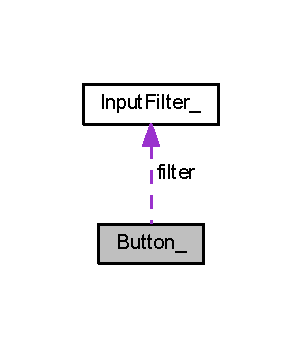
\includegraphics[width=145pt]{struct_button____coll__graph}
\end{center}
\end{figure}
\subsection*{Data Fields}
\begin{DoxyCompactItemize}
\item 
\mbox{\hyperlink{button_8h_aa0f38bbf6320aea7cc99c3a77ed46d80}{Input\+Filter}} $\ast$ \mbox{\hyperlink{struct_button___a9568e563650fcb16283e6df6008722e9}{filter}}
\item 
void($\ast$ \mbox{\hyperlink{struct_button___a54894037c0b758948b3d4d4ac39c2c0c}{sample}} )(struct \mbox{\hyperlink{struct_button__}{Button\+\_\+}} $\ast$const)
\item 
\mbox{\hyperlink{button_8h_a4ef43ff5c6d42dacbc8ffd9c8cfdc189}{edge}}($\ast$ \mbox{\hyperlink{struct_button___a164ee133b5e4233ebd6a6849f806f551}{get\+Edge}} )(struct \mbox{\hyperlink{struct_button__}{Button\+\_\+}} $\ast$const)
\end{DoxyCompactItemize}


\subsection{Detailed Description}


Definition at line 15 of file button.\+h.



\subsection{Field Documentation}
\mbox{\Hypertarget{struct_button___a9568e563650fcb16283e6df6008722e9}\label{struct_button___a9568e563650fcb16283e6df6008722e9}} 
\index{Button\+\_\+@{Button\+\_\+}!filter@{filter}}
\index{filter@{filter}!Button\+\_\+@{Button\+\_\+}}
\subsubsection{\texorpdfstring{filter}{filter}}
{\footnotesize\ttfamily \mbox{\hyperlink{button_8h_aa0f38bbf6320aea7cc99c3a77ed46d80}{Input\+Filter}}$\ast$ filter}



Definition at line 16 of file button.\+h.

\mbox{\Hypertarget{struct_button___a164ee133b5e4233ebd6a6849f806f551}\label{struct_button___a164ee133b5e4233ebd6a6849f806f551}} 
\index{Button\+\_\+@{Button\+\_\+}!get\+Edge@{get\+Edge}}
\index{get\+Edge@{get\+Edge}!Button\+\_\+@{Button\+\_\+}}
\subsubsection{\texorpdfstring{get\+Edge}{getEdge}}
{\footnotesize\ttfamily \mbox{\hyperlink{button_8h_a4ef43ff5c6d42dacbc8ffd9c8cfdc189}{edge}}($\ast$ get\+Edge) (struct \mbox{\hyperlink{struct_button__}{Button\+\_\+}} $\ast$const)}



Definition at line 18 of file button.\+h.

\mbox{\Hypertarget{struct_button___a54894037c0b758948b3d4d4ac39c2c0c}\label{struct_button___a54894037c0b758948b3d4d4ac39c2c0c}} 
\index{Button\+\_\+@{Button\+\_\+}!sample@{sample}}
\index{sample@{sample}!Button\+\_\+@{Button\+\_\+}}
\subsubsection{\texorpdfstring{sample}{sample}}
{\footnotesize\ttfamily void($\ast$ sample) (struct \mbox{\hyperlink{struct_button__}{Button\+\_\+}} $\ast$const)}



Definition at line 17 of file button.\+h.



The documentation for this struct was generated from the following file\+:\begin{DoxyCompactItemize}
\item 
C\+:/\+Users/\+T\+H\+P/\+Desktop/\+Unibern/2018\+\_\+02/\+Subjects/\+Programming\+\_\+\+Microcontroller/\+Paeks/samples/\+My\+\_\+\+Project/\+Library/\+Library/inc/\mbox{\hyperlink{button_8h}{button.\+h}}\end{DoxyCompactItemize}

\hypertarget{union_cool_step_control_register__}{}\section{Cool\+Step\+Control\+Register\+\_\+ Union Reference}
\label{union_cool_step_control_register__}\index{Cool\+Step\+Control\+Register\+\_\+@{Cool\+Step\+Control\+Register\+\_\+}}


{\ttfamily \#include $<$tmc260\+\_\+driver.\+h$>$}

\subsection*{Data Fields}
\begin{DoxyCompactItemize}
\item 
\mbox{\hyperlink{tmc260__driver_8h_a280b01a3b5bb4294fcee278b00c030d6}{Register}} \mbox{\hyperlink{union_cool_step_control_register___a445b72174063a88455cd86c22d77d03f}{bytes}}
\item 
\begin{tabbing}
xx\=xx\=xx\=xx\=xx\=xx\=xx\=xx\=xx\=\kill
struct \{\\
\>uint32\_t \mbox{\hyperlink{union_cool_step_control_register___a9a642405b33c7c5871acdc91b76e022a}{lowerCoolStepThresholdOrCoolStepDisable}}: 4\\
\>uint32\_t \mbox{\hyperlink{union_cool_step_control_register___aa5d9ea4624bf97017a821a70177c6bdb}{reserved\_1}}: 1\\
\>uint32\_t \mbox{\hyperlink{union_cool_step_control_register___a22bf9a9bfb112875af92a16079771f8b}{currentIncrementSize}}: 2\\
\>uint32\_t \mbox{\hyperlink{union_cool_step_control_register___a50b223df92282d04dfa46306b53a9905}{reserved\_2}}: 1\\
\>uint32\_t \mbox{\hyperlink{union_cool_step_control_register___a84ae4a5a201e30da398f39e1a409ee76}{upperCoolStepThresholdAsOffsetFromLower}}: 4\\
\>uint32\_t \mbox{\hyperlink{union_cool_step_control_register___af8407645db2d0329264f3c6d0cbd6dd1}{reserved\_3}}: 1\\
\>uint32\_t \mbox{\hyperlink{union_cool_step_control_register___a6f2d5c619fb9b48315f8a4de1c2e5931}{currentDecrementSpeed}}: 2\\
\>uint32\_t \mbox{\hyperlink{union_cool_step_control_register___af8688794d33927fc968f85c08d9762fa}{minimumCoolStepCurrent}}: 1\\
\>uint32\_t \mbox{\hyperlink{union_cool_step_control_register___aaf2eb7a7615ec891d7e5a9d49d433f37}{reserved\_4}}: 1\\
\>uint32\_t \mbox{\hyperlink{union_cool_step_control_register___a8e58d0701295971bc3d890f5107f8aa5}{registerAdressBit\_1}}: 1\\
\>uint32\_t \mbox{\hyperlink{union_cool_step_control_register___abd6d1c957737511340b85f5c2d61f9ab}{registerAdressBit\_2}}: 1\\
\>uint32\_t \mbox{\hyperlink{union_cool_step_control_register___a3da0387ab629039b91d051ab328910f0}{registerAdressBit\_3}}: 1\\
\>uint32\_t \mbox{\hyperlink{union_cool_step_control_register___a3e57c2ef1c3ffb36722f000cc1156824}{\_\_pad0\_\_}}: 4\\
\} \mbox{\hyperlink{union_cool_step_control_register___a2b4d1a5feeacad886bebe555d2851dea}{bits}}\\

\end{tabbing}\end{DoxyCompactItemize}


\subsection{Detailed Description}
Union to represent the cool\+Step control register (S\+M\+A\+R\+T\+EN) of a tmc260 device as bitfield 

Definition at line 77 of file tmc260\+\_\+driver.\+h.



\subsection{Field Documentation}
\mbox{\Hypertarget{union_cool_step_control_register___a3e57c2ef1c3ffb36722f000cc1156824}\label{union_cool_step_control_register___a3e57c2ef1c3ffb36722f000cc1156824}} 
\index{Cool\+Step\+Control\+Register\+\_\+@{Cool\+Step\+Control\+Register\+\_\+}!\+\_\+\+\_\+pad0\+\_\+\+\_\+@{\+\_\+\+\_\+pad0\+\_\+\+\_\+}}
\index{\+\_\+\+\_\+pad0\+\_\+\+\_\+@{\+\_\+\+\_\+pad0\+\_\+\+\_\+}!Cool\+Step\+Control\+Register\+\_\+@{Cool\+Step\+Control\+Register\+\_\+}}
\subsubsection{\texorpdfstring{\+\_\+\+\_\+pad0\+\_\+\+\_\+}{\_\_pad0\_\_}}
{\footnotesize\ttfamily uint32\+\_\+t \+\_\+\+\_\+pad0\+\_\+\+\_\+}



Definition at line 92 of file tmc260\+\_\+driver.\+h.

\mbox{\Hypertarget{union_cool_step_control_register___a2b4d1a5feeacad886bebe555d2851dea}\label{union_cool_step_control_register___a2b4d1a5feeacad886bebe555d2851dea}} 
\index{Cool\+Step\+Control\+Register\+\_\+@{Cool\+Step\+Control\+Register\+\_\+}!bits@{bits}}
\index{bits@{bits}!Cool\+Step\+Control\+Register\+\_\+@{Cool\+Step\+Control\+Register\+\_\+}}
\subsubsection{\texorpdfstring{bits}{bits}}
{\footnotesize\ttfamily struct \{ ... \}  bits}

\mbox{\Hypertarget{union_cool_step_control_register___a445b72174063a88455cd86c22d77d03f}\label{union_cool_step_control_register___a445b72174063a88455cd86c22d77d03f}} 
\index{Cool\+Step\+Control\+Register\+\_\+@{Cool\+Step\+Control\+Register\+\_\+}!bytes@{bytes}}
\index{bytes@{bytes}!Cool\+Step\+Control\+Register\+\_\+@{Cool\+Step\+Control\+Register\+\_\+}}
\subsubsection{\texorpdfstring{bytes}{bytes}}
{\footnotesize\ttfamily \mbox{\hyperlink{tmc260__driver_8h_a280b01a3b5bb4294fcee278b00c030d6}{Register}} bytes}



Definition at line 78 of file tmc260\+\_\+driver.\+h.

\mbox{\Hypertarget{union_cool_step_control_register___a6f2d5c619fb9b48315f8a4de1c2e5931}\label{union_cool_step_control_register___a6f2d5c619fb9b48315f8a4de1c2e5931}} 
\index{Cool\+Step\+Control\+Register\+\_\+@{Cool\+Step\+Control\+Register\+\_\+}!current\+Decrement\+Speed@{current\+Decrement\+Speed}}
\index{current\+Decrement\+Speed@{current\+Decrement\+Speed}!Cool\+Step\+Control\+Register\+\_\+@{Cool\+Step\+Control\+Register\+\_\+}}
\subsubsection{\texorpdfstring{current\+Decrement\+Speed}{currentDecrementSpeed}}
{\footnotesize\ttfamily uint32\+\_\+t current\+Decrement\+Speed}



Definition at line 86 of file tmc260\+\_\+driver.\+h.

\mbox{\Hypertarget{union_cool_step_control_register___a22bf9a9bfb112875af92a16079771f8b}\label{union_cool_step_control_register___a22bf9a9bfb112875af92a16079771f8b}} 
\index{Cool\+Step\+Control\+Register\+\_\+@{Cool\+Step\+Control\+Register\+\_\+}!current\+Increment\+Size@{current\+Increment\+Size}}
\index{current\+Increment\+Size@{current\+Increment\+Size}!Cool\+Step\+Control\+Register\+\_\+@{Cool\+Step\+Control\+Register\+\_\+}}
\subsubsection{\texorpdfstring{current\+Increment\+Size}{currentIncrementSize}}
{\footnotesize\ttfamily uint32\+\_\+t current\+Increment\+Size}



Definition at line 82 of file tmc260\+\_\+driver.\+h.

\mbox{\Hypertarget{union_cool_step_control_register___a9a642405b33c7c5871acdc91b76e022a}\label{union_cool_step_control_register___a9a642405b33c7c5871acdc91b76e022a}} 
\index{Cool\+Step\+Control\+Register\+\_\+@{Cool\+Step\+Control\+Register\+\_\+}!lower\+Cool\+Step\+Threshold\+Or\+Cool\+Step\+Disable@{lower\+Cool\+Step\+Threshold\+Or\+Cool\+Step\+Disable}}
\index{lower\+Cool\+Step\+Threshold\+Or\+Cool\+Step\+Disable@{lower\+Cool\+Step\+Threshold\+Or\+Cool\+Step\+Disable}!Cool\+Step\+Control\+Register\+\_\+@{Cool\+Step\+Control\+Register\+\_\+}}
\subsubsection{\texorpdfstring{lower\+Cool\+Step\+Threshold\+Or\+Cool\+Step\+Disable}{lowerCoolStepThresholdOrCoolStepDisable}}
{\footnotesize\ttfamily uint32\+\_\+t lower\+Cool\+Step\+Threshold\+Or\+Cool\+Step\+Disable}



Definition at line 80 of file tmc260\+\_\+driver.\+h.

\mbox{\Hypertarget{union_cool_step_control_register___af8688794d33927fc968f85c08d9762fa}\label{union_cool_step_control_register___af8688794d33927fc968f85c08d9762fa}} 
\index{Cool\+Step\+Control\+Register\+\_\+@{Cool\+Step\+Control\+Register\+\_\+}!minimum\+Cool\+Step\+Current@{minimum\+Cool\+Step\+Current}}
\index{minimum\+Cool\+Step\+Current@{minimum\+Cool\+Step\+Current}!Cool\+Step\+Control\+Register\+\_\+@{Cool\+Step\+Control\+Register\+\_\+}}
\subsubsection{\texorpdfstring{minimum\+Cool\+Step\+Current}{minimumCoolStepCurrent}}
{\footnotesize\ttfamily uint32\+\_\+t minimum\+Cool\+Step\+Current}



Definition at line 87 of file tmc260\+\_\+driver.\+h.

\mbox{\Hypertarget{union_cool_step_control_register___a8e58d0701295971bc3d890f5107f8aa5}\label{union_cool_step_control_register___a8e58d0701295971bc3d890f5107f8aa5}} 
\index{Cool\+Step\+Control\+Register\+\_\+@{Cool\+Step\+Control\+Register\+\_\+}!register\+Adress\+Bit\+\_\+1@{register\+Adress\+Bit\+\_\+1}}
\index{register\+Adress\+Bit\+\_\+1@{register\+Adress\+Bit\+\_\+1}!Cool\+Step\+Control\+Register\+\_\+@{Cool\+Step\+Control\+Register\+\_\+}}
\subsubsection{\texorpdfstring{register\+Adress\+Bit\+\_\+1}{registerAdressBit\_1}}
{\footnotesize\ttfamily uint32\+\_\+t register\+Adress\+Bit\+\_\+1}



Definition at line 89 of file tmc260\+\_\+driver.\+h.

\mbox{\Hypertarget{union_cool_step_control_register___abd6d1c957737511340b85f5c2d61f9ab}\label{union_cool_step_control_register___abd6d1c957737511340b85f5c2d61f9ab}} 
\index{Cool\+Step\+Control\+Register\+\_\+@{Cool\+Step\+Control\+Register\+\_\+}!register\+Adress\+Bit\+\_\+2@{register\+Adress\+Bit\+\_\+2}}
\index{register\+Adress\+Bit\+\_\+2@{register\+Adress\+Bit\+\_\+2}!Cool\+Step\+Control\+Register\+\_\+@{Cool\+Step\+Control\+Register\+\_\+}}
\subsubsection{\texorpdfstring{register\+Adress\+Bit\+\_\+2}{registerAdressBit\_2}}
{\footnotesize\ttfamily uint32\+\_\+t register\+Adress\+Bit\+\_\+2}



Definition at line 90 of file tmc260\+\_\+driver.\+h.

\mbox{\Hypertarget{union_cool_step_control_register___a3da0387ab629039b91d051ab328910f0}\label{union_cool_step_control_register___a3da0387ab629039b91d051ab328910f0}} 
\index{Cool\+Step\+Control\+Register\+\_\+@{Cool\+Step\+Control\+Register\+\_\+}!register\+Adress\+Bit\+\_\+3@{register\+Adress\+Bit\+\_\+3}}
\index{register\+Adress\+Bit\+\_\+3@{register\+Adress\+Bit\+\_\+3}!Cool\+Step\+Control\+Register\+\_\+@{Cool\+Step\+Control\+Register\+\_\+}}
\subsubsection{\texorpdfstring{register\+Adress\+Bit\+\_\+3}{registerAdressBit\_3}}
{\footnotesize\ttfamily uint32\+\_\+t register\+Adress\+Bit\+\_\+3}



Definition at line 91 of file tmc260\+\_\+driver.\+h.

\mbox{\Hypertarget{union_cool_step_control_register___aa5d9ea4624bf97017a821a70177c6bdb}\label{union_cool_step_control_register___aa5d9ea4624bf97017a821a70177c6bdb}} 
\index{Cool\+Step\+Control\+Register\+\_\+@{Cool\+Step\+Control\+Register\+\_\+}!reserved\+\_\+1@{reserved\+\_\+1}}
\index{reserved\+\_\+1@{reserved\+\_\+1}!Cool\+Step\+Control\+Register\+\_\+@{Cool\+Step\+Control\+Register\+\_\+}}
\subsubsection{\texorpdfstring{reserved\+\_\+1}{reserved\_1}}
{\footnotesize\ttfamily uint32\+\_\+t reserved\+\_\+1}



Definition at line 81 of file tmc260\+\_\+driver.\+h.

\mbox{\Hypertarget{union_cool_step_control_register___a50b223df92282d04dfa46306b53a9905}\label{union_cool_step_control_register___a50b223df92282d04dfa46306b53a9905}} 
\index{Cool\+Step\+Control\+Register\+\_\+@{Cool\+Step\+Control\+Register\+\_\+}!reserved\+\_\+2@{reserved\+\_\+2}}
\index{reserved\+\_\+2@{reserved\+\_\+2}!Cool\+Step\+Control\+Register\+\_\+@{Cool\+Step\+Control\+Register\+\_\+}}
\subsubsection{\texorpdfstring{reserved\+\_\+2}{reserved\_2}}
{\footnotesize\ttfamily uint32\+\_\+t reserved\+\_\+2}



Definition at line 83 of file tmc260\+\_\+driver.\+h.

\mbox{\Hypertarget{union_cool_step_control_register___af8407645db2d0329264f3c6d0cbd6dd1}\label{union_cool_step_control_register___af8407645db2d0329264f3c6d0cbd6dd1}} 
\index{Cool\+Step\+Control\+Register\+\_\+@{Cool\+Step\+Control\+Register\+\_\+}!reserved\+\_\+3@{reserved\+\_\+3}}
\index{reserved\+\_\+3@{reserved\+\_\+3}!Cool\+Step\+Control\+Register\+\_\+@{Cool\+Step\+Control\+Register\+\_\+}}
\subsubsection{\texorpdfstring{reserved\+\_\+3}{reserved\_3}}
{\footnotesize\ttfamily uint32\+\_\+t reserved\+\_\+3}



Definition at line 85 of file tmc260\+\_\+driver.\+h.

\mbox{\Hypertarget{union_cool_step_control_register___aaf2eb7a7615ec891d7e5a9d49d433f37}\label{union_cool_step_control_register___aaf2eb7a7615ec891d7e5a9d49d433f37}} 
\index{Cool\+Step\+Control\+Register\+\_\+@{Cool\+Step\+Control\+Register\+\_\+}!reserved\+\_\+4@{reserved\+\_\+4}}
\index{reserved\+\_\+4@{reserved\+\_\+4}!Cool\+Step\+Control\+Register\+\_\+@{Cool\+Step\+Control\+Register\+\_\+}}
\subsubsection{\texorpdfstring{reserved\+\_\+4}{reserved\_4}}
{\footnotesize\ttfamily uint32\+\_\+t reserved\+\_\+4}



Definition at line 88 of file tmc260\+\_\+driver.\+h.

\mbox{\Hypertarget{union_cool_step_control_register___a84ae4a5a201e30da398f39e1a409ee76}\label{union_cool_step_control_register___a84ae4a5a201e30da398f39e1a409ee76}} 
\index{Cool\+Step\+Control\+Register\+\_\+@{Cool\+Step\+Control\+Register\+\_\+}!upper\+Cool\+Step\+Threshold\+As\+Offset\+From\+Lower@{upper\+Cool\+Step\+Threshold\+As\+Offset\+From\+Lower}}
\index{upper\+Cool\+Step\+Threshold\+As\+Offset\+From\+Lower@{upper\+Cool\+Step\+Threshold\+As\+Offset\+From\+Lower}!Cool\+Step\+Control\+Register\+\_\+@{Cool\+Step\+Control\+Register\+\_\+}}
\subsubsection{\texorpdfstring{upper\+Cool\+Step\+Threshold\+As\+Offset\+From\+Lower}{upperCoolStepThresholdAsOffsetFromLower}}
{\footnotesize\ttfamily uint32\+\_\+t upper\+Cool\+Step\+Threshold\+As\+Offset\+From\+Lower}



Definition at line 84 of file tmc260\+\_\+driver.\+h.



The documentation for this union was generated from the following file\+:\begin{DoxyCompactItemize}
\item 
Library/\+Library/inc/\mbox{\hyperlink{tmc260__driver_8h}{tmc260\+\_\+driver.\+h}}\end{DoxyCompactItemize}

\hypertarget{struct_data_buffer}{}\section{Data\+Buffer Struct Reference}
\label{struct_data_buffer}\index{Data\+Buffer@{Data\+Buffer}}


{\ttfamily \#include $<$interface\+\_\+\+A\+N\+A\+L\+Y\+S\+I\+S\+\_\+pincinato.\+h$>$}

\subsection*{Data Fields}
\begin{DoxyCompactItemize}
\item 
uint8\+\_\+t \mbox{\hyperlink{struct_data_buffer_aae5a12e607d0f782506d9e6ec6179c64}{index}}
\item 
bool \mbox{\hyperlink{struct_data_buffer_a28b95a576c2cbf8b46a32c572ebd23b9}{actual}}
\item 
uint32\+\_\+t \mbox{\hyperlink{struct_data_buffer_a879b8a6fa7f2626814e9c149bdfc3139}{buf}} \mbox{[}\mbox{\hyperlink{interface___a_n_a_l_y_s_i_s__pincinato_8h_a8d58dfb2133bff91e140c30b2c72ed04}{B\+U\+F\+F\+E\+R\+S\+I\+Z\+E\+A\+N\+A\+L\+Y\+S\+IS}}\mbox{]}
\end{DoxyCompactItemize}


\subsection{Detailed Description}


Definition at line 32 of file interface\+\_\+\+A\+N\+A\+L\+Y\+S\+I\+S\+\_\+pincinato.\+h.



\subsection{Field Documentation}
\mbox{\Hypertarget{struct_data_buffer_a28b95a576c2cbf8b46a32c572ebd23b9}\label{struct_data_buffer_a28b95a576c2cbf8b46a32c572ebd23b9}} 
\index{Data\+Buffer@{Data\+Buffer}!actual@{actual}}
\index{actual@{actual}!Data\+Buffer@{Data\+Buffer}}
\subsubsection{\texorpdfstring{actual}{actual}}
{\footnotesize\ttfamily bool actual}



Definition at line 35 of file interface\+\_\+\+A\+N\+A\+L\+Y\+S\+I\+S\+\_\+pincinato.\+h.

\mbox{\Hypertarget{struct_data_buffer_a879b8a6fa7f2626814e9c149bdfc3139}\label{struct_data_buffer_a879b8a6fa7f2626814e9c149bdfc3139}} 
\index{Data\+Buffer@{Data\+Buffer}!buf@{buf}}
\index{buf@{buf}!Data\+Buffer@{Data\+Buffer}}
\subsubsection{\texorpdfstring{buf}{buf}}
{\footnotesize\ttfamily uint32\+\_\+t buf\mbox{[}\mbox{\hyperlink{interface___a_n_a_l_y_s_i_s__pincinato_8h_a8d58dfb2133bff91e140c30b2c72ed04}{B\+U\+F\+F\+E\+R\+S\+I\+Z\+E\+A\+N\+A\+L\+Y\+S\+IS}}\mbox{]}}



Definition at line 36 of file interface\+\_\+\+A\+N\+A\+L\+Y\+S\+I\+S\+\_\+pincinato.\+h.

\mbox{\Hypertarget{struct_data_buffer_aae5a12e607d0f782506d9e6ec6179c64}\label{struct_data_buffer_aae5a12e607d0f782506d9e6ec6179c64}} 
\index{Data\+Buffer@{Data\+Buffer}!index@{index}}
\index{index@{index}!Data\+Buffer@{Data\+Buffer}}
\subsubsection{\texorpdfstring{index}{index}}
{\footnotesize\ttfamily uint8\+\_\+t index}



Definition at line 34 of file interface\+\_\+\+A\+N\+A\+L\+Y\+S\+I\+S\+\_\+pincinato.\+h.



The documentation for this struct was generated from the following file\+:\begin{DoxyCompactItemize}
\item 
Library/\+Library/inc/\mbox{\hyperlink{interface___a_n_a_l_y_s_i_s__pincinato_8h}{interface\+\_\+\+A\+N\+A\+L\+Y\+S\+I\+S\+\_\+pincinato.\+h}}\end{DoxyCompactItemize}

\hypertarget{struct_data_buffer__}{}\section{Data\+Buffer\+\_\+ Struct Reference}
\label{struct_data_buffer__}\index{Data\+Buffer\+\_\+@{Data\+Buffer\+\_\+}}


{\ttfamily \#include $<$interface\+\_\+\+A\+N\+A\+L\+Y\+S\+I\+S\+\_\+pincinato.\+h$>$}

\subsection*{Data Fields}
\begin{DoxyCompactItemize}
\item 
uint8\+\_\+t \mbox{\hyperlink{struct_data_buffer___aae5a12e607d0f782506d9e6ec6179c64}{index}}
\item 
bool \mbox{\hyperlink{struct_data_buffer___a414d502c8f0c1f140326e0acab1abac2}{buf}} \mbox{[}\mbox{\hyperlink{interface___a_n_a_l_y_s_i_s__pincinato_8h_a15298070513fb95a1e8c82f64628c9ac}{B\+U\+F\+F\+E\+R\+S\+I\+Z\+E\+A\+B\+N\+O\+R\+M\+A\+L\+I\+T\+I\+ES}}\mbox{]}
\end{DoxyCompactItemize}


\subsection{Detailed Description}


Definition at line 39 of file interface\+\_\+\+A\+N\+A\+L\+Y\+S\+I\+S\+\_\+pincinato.\+h.



\subsection{Field Documentation}
\mbox{\Hypertarget{struct_data_buffer___a414d502c8f0c1f140326e0acab1abac2}\label{struct_data_buffer___a414d502c8f0c1f140326e0acab1abac2}} 
\index{Data\+Buffer\+\_\+@{Data\+Buffer\+\_\+}!buf@{buf}}
\index{buf@{buf}!Data\+Buffer\+\_\+@{Data\+Buffer\+\_\+}}
\subsubsection{\texorpdfstring{buf}{buf}}
{\footnotesize\ttfamily bool buf\mbox{[}\mbox{\hyperlink{interface___a_n_a_l_y_s_i_s__pincinato_8h_a15298070513fb95a1e8c82f64628c9ac}{B\+U\+F\+F\+E\+R\+S\+I\+Z\+E\+A\+B\+N\+O\+R\+M\+A\+L\+I\+T\+I\+ES}}\mbox{]}}



Definition at line 42 of file interface\+\_\+\+A\+N\+A\+L\+Y\+S\+I\+S\+\_\+pincinato.\+h.

\mbox{\Hypertarget{struct_data_buffer___aae5a12e607d0f782506d9e6ec6179c64}\label{struct_data_buffer___aae5a12e607d0f782506d9e6ec6179c64}} 
\index{Data\+Buffer\+\_\+@{Data\+Buffer\+\_\+}!index@{index}}
\index{index@{index}!Data\+Buffer\+\_\+@{Data\+Buffer\+\_\+}}
\subsubsection{\texorpdfstring{index}{index}}
{\footnotesize\ttfamily uint8\+\_\+t index}



Definition at line 41 of file interface\+\_\+\+A\+N\+A\+L\+Y\+S\+I\+S\+\_\+pincinato.\+h.



The documentation for this struct was generated from the following file\+:\begin{DoxyCompactItemize}
\item 
Library/\+Library/inc/\mbox{\hyperlink{interface___a_n_a_l_y_s_i_s__pincinato_8h}{interface\+\_\+\+A\+N\+A\+L\+Y\+S\+I\+S\+\_\+pincinato.\+h}}\end{DoxyCompactItemize}

\hypertarget{struct_data_process______}{}\section{Data\+Process\+\_\+\+\_\+\+\_\+ Struct Reference}
\label{struct_data_process______}\index{Data\+Process\+\_\+\+\_\+\+\_\+@{Data\+Process\+\_\+\+\_\+\+\_\+}}


{\ttfamily \#include $<$interface\+\_\+\+A\+N\+A\+L\+Y\+S\+I\+S\+\_\+pincinato.\+h$>$}



Collaboration diagram for Data\+Process\+\_\+\+\_\+\+\_\+\+:\nopagebreak
\begin{figure}[H]
\begin{center}
\leavevmode
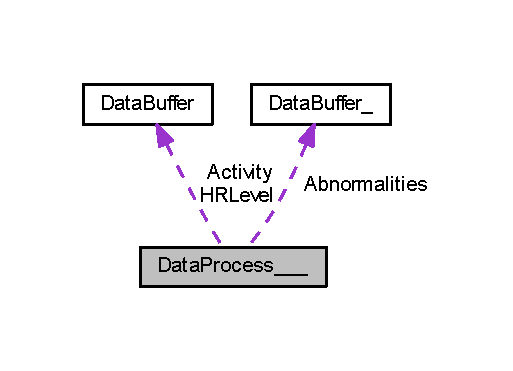
\includegraphics[width=246pt]{struct_data_process________coll__graph}
\end{center}
\end{figure}
\subsection*{Data Fields}
\begin{DoxyCompactItemize}
\item 
\mbox{\hyperlink{interface___a_n_a_l_y_s_i_s__pincinato_8h_a3184f2c2dc500ffc383f0a5e8e7f21f0}{my\+Buffer}} \mbox{\hyperlink{struct_data_process_______a696c2caf522a9390d98922952a57670f}{Activity}}
\item 
\mbox{\hyperlink{interface___a_n_a_l_y_s_i_s__pincinato_8h_a3184f2c2dc500ffc383f0a5e8e7f21f0}{my\+Buffer}} \mbox{\hyperlink{struct_data_process_______af6130eb725e93603b2960dec4d4378ff}{H\+R\+Level}}
\item 
\mbox{\hyperlink{interface___a_n_a_l_y_s_i_s__pincinato_8h_a02b20b214e8ea5dba5c4b81cd4638fc1}{my\+Buffer\+\_\+}} \mbox{\hyperlink{struct_data_process_______a9d2c0e8b260cec8c51618e7991a2c787}{Abnormalities}}
\end{DoxyCompactItemize}


\subsection{Detailed Description}


Definition at line 46 of file interface\+\_\+\+A\+N\+A\+L\+Y\+S\+I\+S\+\_\+pincinato.\+h.



\subsection{Field Documentation}
\mbox{\Hypertarget{struct_data_process_______a9d2c0e8b260cec8c51618e7991a2c787}\label{struct_data_process_______a9d2c0e8b260cec8c51618e7991a2c787}} 
\index{Data\+Process\+\_\+\+\_\+\+\_\+@{Data\+Process\+\_\+\+\_\+\+\_\+}!Abnormalities@{Abnormalities}}
\index{Abnormalities@{Abnormalities}!Data\+Process\+\_\+\+\_\+\+\_\+@{Data\+Process\+\_\+\+\_\+\+\_\+}}
\subsubsection{\texorpdfstring{Abnormalities}{Abnormalities}}
{\footnotesize\ttfamily \mbox{\hyperlink{interface___a_n_a_l_y_s_i_s__pincinato_8h_a02b20b214e8ea5dba5c4b81cd4638fc1}{my\+Buffer\+\_\+}} Abnormalities}



Definition at line 50 of file interface\+\_\+\+A\+N\+A\+L\+Y\+S\+I\+S\+\_\+pincinato.\+h.

\mbox{\Hypertarget{struct_data_process_______a696c2caf522a9390d98922952a57670f}\label{struct_data_process_______a696c2caf522a9390d98922952a57670f}} 
\index{Data\+Process\+\_\+\+\_\+\+\_\+@{Data\+Process\+\_\+\+\_\+\+\_\+}!Activity@{Activity}}
\index{Activity@{Activity}!Data\+Process\+\_\+\+\_\+\+\_\+@{Data\+Process\+\_\+\+\_\+\+\_\+}}
\subsubsection{\texorpdfstring{Activity}{Activity}}
{\footnotesize\ttfamily \mbox{\hyperlink{interface___a_n_a_l_y_s_i_s__pincinato_8h_a3184f2c2dc500ffc383f0a5e8e7f21f0}{my\+Buffer}} Activity}



Definition at line 48 of file interface\+\_\+\+A\+N\+A\+L\+Y\+S\+I\+S\+\_\+pincinato.\+h.

\mbox{\Hypertarget{struct_data_process_______af6130eb725e93603b2960dec4d4378ff}\label{struct_data_process_______af6130eb725e93603b2960dec4d4378ff}} 
\index{Data\+Process\+\_\+\+\_\+\+\_\+@{Data\+Process\+\_\+\+\_\+\+\_\+}!H\+R\+Level@{H\+R\+Level}}
\index{H\+R\+Level@{H\+R\+Level}!Data\+Process\+\_\+\+\_\+\+\_\+@{Data\+Process\+\_\+\+\_\+\+\_\+}}
\subsubsection{\texorpdfstring{H\+R\+Level}{HRLevel}}
{\footnotesize\ttfamily \mbox{\hyperlink{interface___a_n_a_l_y_s_i_s__pincinato_8h_a3184f2c2dc500ffc383f0a5e8e7f21f0}{my\+Buffer}} H\+R\+Level}



Definition at line 49 of file interface\+\_\+\+A\+N\+A\+L\+Y\+S\+I\+S\+\_\+pincinato.\+h.



The documentation for this struct was generated from the following file\+:\begin{DoxyCompactItemize}
\item 
Library/\+Library/inc/\mbox{\hyperlink{interface___a_n_a_l_y_s_i_s__pincinato_8h}{interface\+\_\+\+A\+N\+A\+L\+Y\+S\+I\+S\+\_\+pincinato.\+h}}\end{DoxyCompactItemize}

\hypertarget{struct_input_filter__}{}\section{Input\+Filter\+\_\+ Struct Reference}
\label{struct_input_filter__}\index{Input\+Filter\+\_\+@{Input\+Filter\+\_\+}}


{\ttfamily \#include $<$button\+\_\+driver.\+h$>$}

\subsection*{Data Fields}
\begin{DoxyCompactItemize}
\item 
uint16\+\_\+t \mbox{\hyperlink{struct_input_filter___a295d2f6601495531b475a5965dd36c4b}{raw\+Input\+Set}}
\item 
bool \mbox{\hyperlink{struct_input_filter___a2e42fdbabb33aea9674a2f8f378ccd64}{input\+State}}
\item 
\mbox{\hyperlink{button_8h_a4ef43ff5c6d42dacbc8ffd9c8cfdc189}{edge}} \mbox{\hyperlink{struct_input_filter___a54118ea5021c85ed6693f0c268532b24}{pending\+Edge}}
\item 
G\+P\+I\+O\+\_\+\+Type\+Def $\ast$ \mbox{\hyperlink{struct_input_filter___a82241972e0292c7de95ea1e293e11be3}{port}}
\item 
uint16\+\_\+t \mbox{\hyperlink{struct_input_filter___a4144813adfa4dfe7e7cbeea17d1b06eb}{pin}}
\item 
void($\ast$ \mbox{\hyperlink{struct_input_filter___aa2061c47d432d006a5b91e831536710a}{sample}} )(struct \mbox{\hyperlink{struct_input_filter__}{Input\+Filter\+\_\+}} $\ast$const)
\item 
\mbox{\hyperlink{button_8h_a4ef43ff5c6d42dacbc8ffd9c8cfdc189}{edge}}($\ast$ \mbox{\hyperlink{struct_input_filter___a8fc896b9de0dd00ebe329df597dbc9e1}{get\+Edge}} )(struct \mbox{\hyperlink{struct_input_filter__}{Input\+Filter\+\_\+}} $\ast$const)
\end{DoxyCompactItemize}


\subsection{Detailed Description}


Definition at line 18 of file button\+\_\+driver.\+h.



\subsection{Field Documentation}
\mbox{\Hypertarget{struct_input_filter___a8fc896b9de0dd00ebe329df597dbc9e1}\label{struct_input_filter___a8fc896b9de0dd00ebe329df597dbc9e1}} 
\index{Input\+Filter\+\_\+@{Input\+Filter\+\_\+}!get\+Edge@{get\+Edge}}
\index{get\+Edge@{get\+Edge}!Input\+Filter\+\_\+@{Input\+Filter\+\_\+}}
\subsubsection{\texorpdfstring{get\+Edge}{getEdge}}
{\footnotesize\ttfamily \mbox{\hyperlink{button_8h_a4ef43ff5c6d42dacbc8ffd9c8cfdc189}{edge}}($\ast$ get\+Edge) (struct \mbox{\hyperlink{struct_input_filter__}{Input\+Filter\+\_\+}} $\ast$const)}



Definition at line 25 of file button\+\_\+driver.\+h.

\mbox{\Hypertarget{struct_input_filter___a2e42fdbabb33aea9674a2f8f378ccd64}\label{struct_input_filter___a2e42fdbabb33aea9674a2f8f378ccd64}} 
\index{Input\+Filter\+\_\+@{Input\+Filter\+\_\+}!input\+State@{input\+State}}
\index{input\+State@{input\+State}!Input\+Filter\+\_\+@{Input\+Filter\+\_\+}}
\subsubsection{\texorpdfstring{input\+State}{inputState}}
{\footnotesize\ttfamily bool input\+State}



Definition at line 20 of file button\+\_\+driver.\+h.

\mbox{\Hypertarget{struct_input_filter___a54118ea5021c85ed6693f0c268532b24}\label{struct_input_filter___a54118ea5021c85ed6693f0c268532b24}} 
\index{Input\+Filter\+\_\+@{Input\+Filter\+\_\+}!pending\+Edge@{pending\+Edge}}
\index{pending\+Edge@{pending\+Edge}!Input\+Filter\+\_\+@{Input\+Filter\+\_\+}}
\subsubsection{\texorpdfstring{pending\+Edge}{pendingEdge}}
{\footnotesize\ttfamily \mbox{\hyperlink{button_8h_a4ef43ff5c6d42dacbc8ffd9c8cfdc189}{edge}} pending\+Edge}



Definition at line 21 of file button\+\_\+driver.\+h.

\mbox{\Hypertarget{struct_input_filter___a4144813adfa4dfe7e7cbeea17d1b06eb}\label{struct_input_filter___a4144813adfa4dfe7e7cbeea17d1b06eb}} 
\index{Input\+Filter\+\_\+@{Input\+Filter\+\_\+}!pin@{pin}}
\index{pin@{pin}!Input\+Filter\+\_\+@{Input\+Filter\+\_\+}}
\subsubsection{\texorpdfstring{pin}{pin}}
{\footnotesize\ttfamily uint16\+\_\+t pin}



Definition at line 23 of file button\+\_\+driver.\+h.

\mbox{\Hypertarget{struct_input_filter___a82241972e0292c7de95ea1e293e11be3}\label{struct_input_filter___a82241972e0292c7de95ea1e293e11be3}} 
\index{Input\+Filter\+\_\+@{Input\+Filter\+\_\+}!port@{port}}
\index{port@{port}!Input\+Filter\+\_\+@{Input\+Filter\+\_\+}}
\subsubsection{\texorpdfstring{port}{port}}
{\footnotesize\ttfamily G\+P\+I\+O\+\_\+\+Type\+Def$\ast$ port}



Definition at line 22 of file button\+\_\+driver.\+h.

\mbox{\Hypertarget{struct_input_filter___a295d2f6601495531b475a5965dd36c4b}\label{struct_input_filter___a295d2f6601495531b475a5965dd36c4b}} 
\index{Input\+Filter\+\_\+@{Input\+Filter\+\_\+}!raw\+Input\+Set@{raw\+Input\+Set}}
\index{raw\+Input\+Set@{raw\+Input\+Set}!Input\+Filter\+\_\+@{Input\+Filter\+\_\+}}
\subsubsection{\texorpdfstring{raw\+Input\+Set}{rawInputSet}}
{\footnotesize\ttfamily uint16\+\_\+t raw\+Input\+Set}



Definition at line 19 of file button\+\_\+driver.\+h.

\mbox{\Hypertarget{struct_input_filter___aa2061c47d432d006a5b91e831536710a}\label{struct_input_filter___aa2061c47d432d006a5b91e831536710a}} 
\index{Input\+Filter\+\_\+@{Input\+Filter\+\_\+}!sample@{sample}}
\index{sample@{sample}!Input\+Filter\+\_\+@{Input\+Filter\+\_\+}}
\subsubsection{\texorpdfstring{sample}{sample}}
{\footnotesize\ttfamily void($\ast$ sample) (struct \mbox{\hyperlink{struct_input_filter__}{Input\+Filter\+\_\+}} $\ast$const)}



Definition at line 24 of file button\+\_\+driver.\+h.



The documentation for this struct was generated from the following file\+:\begin{DoxyCompactItemize}
\item 
C\+:/\+Users/\+T\+H\+P/\+Desktop/\+Unibern/2018\+\_\+02/\+Subjects/\+Programming\+\_\+\+Microcontroller/\+Paeks/samples/\+My\+\_\+\+Project/\+Library/\+Library/inc/\mbox{\hyperlink{button__driver_8h}{button\+\_\+driver.\+h}}\end{DoxyCompactItemize}

\hypertarget{struct_joystick__}{}\section{Joystick\+\_\+ Struct Reference}
\label{struct_joystick__}\index{Joystick\+\_\+@{Joystick\+\_\+}}


{\ttfamily \#include $<$joystick.\+h$>$}



Collaboration diagram for Joystick\+\_\+\+:\nopagebreak
\begin{figure}[H]
\begin{center}
\leavevmode
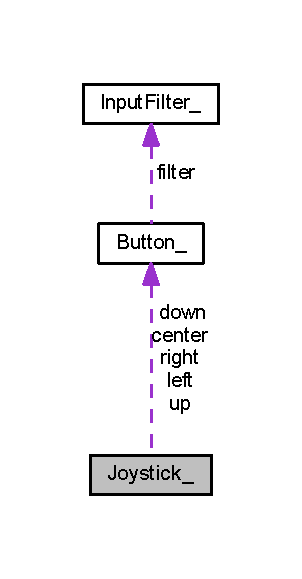
\includegraphics[width=145pt]{struct_joystick____coll__graph}
\end{center}
\end{figure}
\subsection*{Data Fields}
\begin{DoxyCompactItemize}
\item 
\mbox{\hyperlink{button_8h_ab369ab7fa0b9a8dfec4fc1f653ac6de5}{Button}} $\ast$ \mbox{\hyperlink{struct_joystick___aae2bb22ae710c823853d95ae7057884e}{up}}
\item 
\mbox{\hyperlink{button_8h_ab369ab7fa0b9a8dfec4fc1f653ac6de5}{Button}} $\ast$ \mbox{\hyperlink{struct_joystick___a9031d6ddde18c7b16c3242e403f3fbce}{down}}
\item 
\mbox{\hyperlink{button_8h_ab369ab7fa0b9a8dfec4fc1f653ac6de5}{Button}} $\ast$ \mbox{\hyperlink{struct_joystick___a571327757de519da4471010fe0d1e2c5}{left}}
\item 
\mbox{\hyperlink{button_8h_ab369ab7fa0b9a8dfec4fc1f653ac6de5}{Button}} $\ast$ \mbox{\hyperlink{struct_joystick___aa9275d605c1c2da3651589e1d55f9a1a}{right}}
\item 
\mbox{\hyperlink{button_8h_ab369ab7fa0b9a8dfec4fc1f653ac6de5}{Button}} $\ast$ \mbox{\hyperlink{struct_joystick___aa3ad087af028303e400a233a45d87aa2}{center}}
\item 
void($\ast$ \mbox{\hyperlink{struct_joystick___ad68253aed96c4f9e100a9fe238eea009}{sample}} )(struct \mbox{\hyperlink{struct_joystick__}{Joystick\+\_\+}} $\ast$const)
\item 
\mbox{\hyperlink{joystick_8h_ae3f9f641c46a8d3110940cc41d5a50c3}{joystick\+Direction}}($\ast$ \mbox{\hyperlink{struct_joystick___a95b0c18851cf4ff20aedac4196da5e17}{get\+Direction}} )(struct \mbox{\hyperlink{struct_joystick__}{Joystick\+\_\+}} $\ast$const)
\end{DoxyCompactItemize}


\subsection{Detailed Description}


Definition at line 9 of file joystick.\+h.



\subsection{Field Documentation}
\mbox{\Hypertarget{struct_joystick___aa3ad087af028303e400a233a45d87aa2}\label{struct_joystick___aa3ad087af028303e400a233a45d87aa2}} 
\index{Joystick\+\_\+@{Joystick\+\_\+}!center@{center}}
\index{center@{center}!Joystick\+\_\+@{Joystick\+\_\+}}
\subsubsection{\texorpdfstring{center}{center}}
{\footnotesize\ttfamily \mbox{\hyperlink{button_8h_ab369ab7fa0b9a8dfec4fc1f653ac6de5}{Button}}$\ast$ center}



Definition at line 14 of file joystick.\+h.

\mbox{\Hypertarget{struct_joystick___a9031d6ddde18c7b16c3242e403f3fbce}\label{struct_joystick___a9031d6ddde18c7b16c3242e403f3fbce}} 
\index{Joystick\+\_\+@{Joystick\+\_\+}!down@{down}}
\index{down@{down}!Joystick\+\_\+@{Joystick\+\_\+}}
\subsubsection{\texorpdfstring{down}{down}}
{\footnotesize\ttfamily \mbox{\hyperlink{button_8h_ab369ab7fa0b9a8dfec4fc1f653ac6de5}{Button}}$\ast$ down}



Definition at line 11 of file joystick.\+h.

\mbox{\Hypertarget{struct_joystick___a95b0c18851cf4ff20aedac4196da5e17}\label{struct_joystick___a95b0c18851cf4ff20aedac4196da5e17}} 
\index{Joystick\+\_\+@{Joystick\+\_\+}!get\+Direction@{get\+Direction}}
\index{get\+Direction@{get\+Direction}!Joystick\+\_\+@{Joystick\+\_\+}}
\subsubsection{\texorpdfstring{get\+Direction}{getDirection}}
{\footnotesize\ttfamily \mbox{\hyperlink{joystick_8h_ae3f9f641c46a8d3110940cc41d5a50c3}{joystick\+Direction}}($\ast$ get\+Direction) (struct \mbox{\hyperlink{struct_joystick__}{Joystick\+\_\+}} $\ast$const)}



Definition at line 16 of file joystick.\+h.

\mbox{\Hypertarget{struct_joystick___a571327757de519da4471010fe0d1e2c5}\label{struct_joystick___a571327757de519da4471010fe0d1e2c5}} 
\index{Joystick\+\_\+@{Joystick\+\_\+}!left@{left}}
\index{left@{left}!Joystick\+\_\+@{Joystick\+\_\+}}
\subsubsection{\texorpdfstring{left}{left}}
{\footnotesize\ttfamily \mbox{\hyperlink{button_8h_ab369ab7fa0b9a8dfec4fc1f653ac6de5}{Button}}$\ast$ left}



Definition at line 12 of file joystick.\+h.

\mbox{\Hypertarget{struct_joystick___aa9275d605c1c2da3651589e1d55f9a1a}\label{struct_joystick___aa9275d605c1c2da3651589e1d55f9a1a}} 
\index{Joystick\+\_\+@{Joystick\+\_\+}!right@{right}}
\index{right@{right}!Joystick\+\_\+@{Joystick\+\_\+}}
\subsubsection{\texorpdfstring{right}{right}}
{\footnotesize\ttfamily \mbox{\hyperlink{button_8h_ab369ab7fa0b9a8dfec4fc1f653ac6de5}{Button}}$\ast$ right}



Definition at line 13 of file joystick.\+h.

\mbox{\Hypertarget{struct_joystick___ad68253aed96c4f9e100a9fe238eea009}\label{struct_joystick___ad68253aed96c4f9e100a9fe238eea009}} 
\index{Joystick\+\_\+@{Joystick\+\_\+}!sample@{sample}}
\index{sample@{sample}!Joystick\+\_\+@{Joystick\+\_\+}}
\subsubsection{\texorpdfstring{sample}{sample}}
{\footnotesize\ttfamily void($\ast$ sample) (struct \mbox{\hyperlink{struct_joystick__}{Joystick\+\_\+}} $\ast$const)}



Definition at line 15 of file joystick.\+h.

\mbox{\Hypertarget{struct_joystick___aae2bb22ae710c823853d95ae7057884e}\label{struct_joystick___aae2bb22ae710c823853d95ae7057884e}} 
\index{Joystick\+\_\+@{Joystick\+\_\+}!up@{up}}
\index{up@{up}!Joystick\+\_\+@{Joystick\+\_\+}}
\subsubsection{\texorpdfstring{up}{up}}
{\footnotesize\ttfamily \mbox{\hyperlink{button_8h_ab369ab7fa0b9a8dfec4fc1f653ac6de5}{Button}}$\ast$ up}



Definition at line 10 of file joystick.\+h.



The documentation for this struct was generated from the following file\+:\begin{DoxyCompactItemize}
\item 
C\+:/\+Users/\+T\+H\+P/\+Desktop/\+Unibern/2018\+\_\+02/\+Subjects/\+Programming\+\_\+\+Microcontroller/\+Paeks/samples/\+My\+\_\+\+Project/\+Library/\+Library/inc/\mbox{\hyperlink{joystick_8h}{joystick.\+h}}\end{DoxyCompactItemize}

\hypertarget{struct_menu__}{}\section{Menu\+\_\+ Struct Reference}
\label{struct_menu__}\index{Menu\+\_\+@{Menu\+\_\+}}


{\ttfamily \#include $<$lcd\+\_\+menu.\+h$>$}



Collaboration diagram for Menu\+\_\+\+:\nopagebreak
\begin{figure}[H]
\begin{center}
\leavevmode
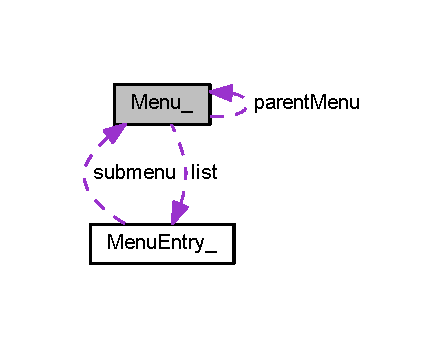
\includegraphics[width=214pt]{struct_menu____coll__graph}
\end{center}
\end{figure}
\subsection*{Data Fields}
\begin{DoxyCompactItemize}
\item 
char const  $\ast$ \mbox{\hyperlink{struct_menu___af92f126a07a2944ef81db37d6e6e21ae}{description}}
\item 
uint8\+\_\+t \mbox{\hyperlink{struct_menu___a4f106d3cb8ba7865c1972731deaf6d45}{number\+Of\+Entries}}
\item 
\mbox{\hyperlink{lcd__menu_8h_a5562b957d336dc1492f008e49dac5f5d}{Menu\+Entry}} $\ast$$\ast$ \mbox{\hyperlink{struct_menu___af3f1ad2de60356d88ae4151e60a87260}{list}}
\item 
\mbox{\hyperlink{lcd__menu_8h_afe0ab1c0311f677767b1588296b0f563}{Menu}} $\ast$ \mbox{\hyperlink{struct_menu___af153fe0e8d7a80232bc537bd3d99d14a}{parent\+Menu}}
\item 
uint8\+\_\+t \mbox{\hyperlink{struct_menu___a0d0cde5c12c27aa95e12e069cae5bdce}{cursor\+Position}}
\item 
uint8\+\_\+t \mbox{\hyperlink{struct_menu___ade32708e7d25a18c52ef9ea43022157e}{page\+Anchor}}
\end{DoxyCompactItemize}


\subsection{Detailed Description}


Definition at line 38 of file lcd\+\_\+menu.\+h.



\subsection{Field Documentation}
\mbox{\Hypertarget{struct_menu___a0d0cde5c12c27aa95e12e069cae5bdce}\label{struct_menu___a0d0cde5c12c27aa95e12e069cae5bdce}} 
\index{Menu\+\_\+@{Menu\+\_\+}!cursor\+Position@{cursor\+Position}}
\index{cursor\+Position@{cursor\+Position}!Menu\+\_\+@{Menu\+\_\+}}
\subsubsection{\texorpdfstring{cursor\+Position}{cursorPosition}}
{\footnotesize\ttfamily uint8\+\_\+t cursor\+Position}



Definition at line 45 of file lcd\+\_\+menu.\+h.

\mbox{\Hypertarget{struct_menu___af92f126a07a2944ef81db37d6e6e21ae}\label{struct_menu___af92f126a07a2944ef81db37d6e6e21ae}} 
\index{Menu\+\_\+@{Menu\+\_\+}!description@{description}}
\index{description@{description}!Menu\+\_\+@{Menu\+\_\+}}
\subsubsection{\texorpdfstring{description}{description}}
{\footnotesize\ttfamily char const$\ast$ description}



Definition at line 40 of file lcd\+\_\+menu.\+h.

\mbox{\Hypertarget{struct_menu___af3f1ad2de60356d88ae4151e60a87260}\label{struct_menu___af3f1ad2de60356d88ae4151e60a87260}} 
\index{Menu\+\_\+@{Menu\+\_\+}!list@{list}}
\index{list@{list}!Menu\+\_\+@{Menu\+\_\+}}
\subsubsection{\texorpdfstring{list}{list}}
{\footnotesize\ttfamily \mbox{\hyperlink{lcd__menu_8h_a5562b957d336dc1492f008e49dac5f5d}{Menu\+Entry}}$\ast$$\ast$ list}



Definition at line 42 of file lcd\+\_\+menu.\+h.

\mbox{\Hypertarget{struct_menu___a4f106d3cb8ba7865c1972731deaf6d45}\label{struct_menu___a4f106d3cb8ba7865c1972731deaf6d45}} 
\index{Menu\+\_\+@{Menu\+\_\+}!number\+Of\+Entries@{number\+Of\+Entries}}
\index{number\+Of\+Entries@{number\+Of\+Entries}!Menu\+\_\+@{Menu\+\_\+}}
\subsubsection{\texorpdfstring{number\+Of\+Entries}{numberOfEntries}}
{\footnotesize\ttfamily uint8\+\_\+t number\+Of\+Entries}



Definition at line 41 of file lcd\+\_\+menu.\+h.

\mbox{\Hypertarget{struct_menu___ade32708e7d25a18c52ef9ea43022157e}\label{struct_menu___ade32708e7d25a18c52ef9ea43022157e}} 
\index{Menu\+\_\+@{Menu\+\_\+}!page\+Anchor@{page\+Anchor}}
\index{page\+Anchor@{page\+Anchor}!Menu\+\_\+@{Menu\+\_\+}}
\subsubsection{\texorpdfstring{page\+Anchor}{pageAnchor}}
{\footnotesize\ttfamily uint8\+\_\+t page\+Anchor}



Definition at line 46 of file lcd\+\_\+menu.\+h.

\mbox{\Hypertarget{struct_menu___af153fe0e8d7a80232bc537bd3d99d14a}\label{struct_menu___af153fe0e8d7a80232bc537bd3d99d14a}} 
\index{Menu\+\_\+@{Menu\+\_\+}!parent\+Menu@{parent\+Menu}}
\index{parent\+Menu@{parent\+Menu}!Menu\+\_\+@{Menu\+\_\+}}
\subsubsection{\texorpdfstring{parent\+Menu}{parentMenu}}
{\footnotesize\ttfamily \mbox{\hyperlink{lcd__menu_8h_afe0ab1c0311f677767b1588296b0f563}{Menu}}$\ast$ parent\+Menu}



Definition at line 44 of file lcd\+\_\+menu.\+h.



The documentation for this struct was generated from the following file\+:\begin{DoxyCompactItemize}
\item 
C\+:/\+Users/\+T\+H\+P/\+Desktop/\+Unibern/2018\+\_\+02/\+Subjects/\+Programming\+\_\+\+Microcontroller/\+Paeks/samples/\+My\+\_\+\+Project/\+Library/\+Library/inc/\mbox{\hyperlink{lcd__menu_8h}{lcd\+\_\+menu.\+h}}\end{DoxyCompactItemize}

\hypertarget{struct_menu_entry__}{}\section{Menu\+Entry\+\_\+ Struct Reference}
\label{struct_menu_entry__}\index{Menu\+Entry\+\_\+@{Menu\+Entry\+\_\+}}


{\ttfamily \#include $<$lcd\+\_\+menu.\+h$>$}



Collaboration diagram for Menu\+Entry\+\_\+\+:\nopagebreak
\begin{figure}[H]
\begin{center}
\leavevmode
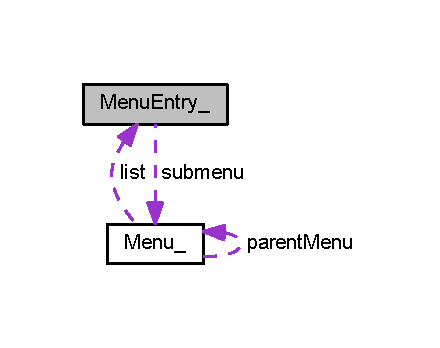
\includegraphics[width=211pt]{struct_menu_entry____coll__graph}
\end{center}
\end{figure}
\subsection*{Data Fields}
\begin{DoxyCompactItemize}
\item 
char const  $\ast$ \mbox{\hyperlink{struct_menu_entry___af92f126a07a2944ef81db37d6e6e21ae}{description}}
\item 
\mbox{\hyperlink{lcd__menu_8h_a8803db0b2985fc11bdaaff101b1b999d}{menu\+\_\+entry\+Type}} \mbox{\hyperlink{struct_menu_entry___a9cb8b226841d530cb28f3763c539bf19}{type}}
\item 
\begin{tabbing}
xx\=xx\=xx\=xx\=xx\=xx\=xx\=xx\=xx\=\kill
union \{\\
\>\mbox{\hyperlink{lcd__menu_8h_afe0ab1c0311f677767b1588296b0f563}{Menu}} $\ast$ \mbox{\hyperlink{struct_menu_entry___a95d149f99e4a49c9b217e31e0289c696}{submenu}}\\
\>\mbox{\hyperlink{lcd__menu_8h_af281888756940391027a7bdddf347718}{menu\_event}} \mbox{\hyperlink{struct_menu_entry___aab46a1780779046bc38a2421e1b9dd36}{event}}\\
\>char const  $\ast$ \mbox{\hyperlink{struct_menu_entry___a02edaa08d1665685fd949ffa77675ef2}{liveData}}\\
\}; \\

\end{tabbing}\end{DoxyCompactItemize}


\subsection{Detailed Description}


Definition at line 27 of file lcd\+\_\+menu.\+h.



\subsection{Field Documentation}
\mbox{\Hypertarget{struct_menu_entry___a59f9cb02ab5a1313406f1e2cd170f5e3}\label{struct_menu_entry___a59f9cb02ab5a1313406f1e2cd170f5e3}} 
\subsubsection{\texorpdfstring{"@1}{@1}}
{\footnotesize\ttfamily union \{ ... \} }

\mbox{\Hypertarget{struct_menu_entry___af92f126a07a2944ef81db37d6e6e21ae}\label{struct_menu_entry___af92f126a07a2944ef81db37d6e6e21ae}} 
\index{Menu\+Entry\+\_\+@{Menu\+Entry\+\_\+}!description@{description}}
\index{description@{description}!Menu\+Entry\+\_\+@{Menu\+Entry\+\_\+}}
\subsubsection{\texorpdfstring{description}{description}}
{\footnotesize\ttfamily char const$\ast$ description}



Definition at line 28 of file lcd\+\_\+menu.\+h.

\mbox{\Hypertarget{struct_menu_entry___aab46a1780779046bc38a2421e1b9dd36}\label{struct_menu_entry___aab46a1780779046bc38a2421e1b9dd36}} 
\index{Menu\+Entry\+\_\+@{Menu\+Entry\+\_\+}!event@{event}}
\index{event@{event}!Menu\+Entry\+\_\+@{Menu\+Entry\+\_\+}}
\subsubsection{\texorpdfstring{event}{event}}
{\footnotesize\ttfamily \mbox{\hyperlink{lcd__menu_8h_af281888756940391027a7bdddf347718}{menu\+\_\+event}} event}



Definition at line 32 of file lcd\+\_\+menu.\+h.

\mbox{\Hypertarget{struct_menu_entry___a02edaa08d1665685fd949ffa77675ef2}\label{struct_menu_entry___a02edaa08d1665685fd949ffa77675ef2}} 
\index{Menu\+Entry\+\_\+@{Menu\+Entry\+\_\+}!live\+Data@{live\+Data}}
\index{live\+Data@{live\+Data}!Menu\+Entry\+\_\+@{Menu\+Entry\+\_\+}}
\subsubsection{\texorpdfstring{live\+Data}{liveData}}
{\footnotesize\ttfamily char const$\ast$ live\+Data}



Definition at line 34 of file lcd\+\_\+menu.\+h.

\mbox{\Hypertarget{struct_menu_entry___a95d149f99e4a49c9b217e31e0289c696}\label{struct_menu_entry___a95d149f99e4a49c9b217e31e0289c696}} 
\index{Menu\+Entry\+\_\+@{Menu\+Entry\+\_\+}!submenu@{submenu}}
\index{submenu@{submenu}!Menu\+Entry\+\_\+@{Menu\+Entry\+\_\+}}
\subsubsection{\texorpdfstring{submenu}{submenu}}
{\footnotesize\ttfamily \mbox{\hyperlink{lcd__menu_8h_afe0ab1c0311f677767b1588296b0f563}{Menu}}$\ast$ submenu}



Definition at line 31 of file lcd\+\_\+menu.\+h.

\mbox{\Hypertarget{struct_menu_entry___a9cb8b226841d530cb28f3763c539bf19}\label{struct_menu_entry___a9cb8b226841d530cb28f3763c539bf19}} 
\index{Menu\+Entry\+\_\+@{Menu\+Entry\+\_\+}!type@{type}}
\index{type@{type}!Menu\+Entry\+\_\+@{Menu\+Entry\+\_\+}}
\subsubsection{\texorpdfstring{type}{type}}
{\footnotesize\ttfamily \mbox{\hyperlink{lcd__menu_8h_a8803db0b2985fc11bdaaff101b1b999d}{menu\+\_\+entry\+Type}} type}



Definition at line 29 of file lcd\+\_\+menu.\+h.



The documentation for this struct was generated from the following file\+:\begin{DoxyCompactItemize}
\item 
C\+:/\+Users/\+T\+H\+P/\+Desktop/\+Unibern/2018\+\_\+02/\+Subjects/\+Programming\+\_\+\+Microcontroller/\+Paeks/samples/\+My\+\_\+\+Project/\+Library/\+Library/inc/\mbox{\hyperlink{lcd__menu_8h}{lcd\+\_\+menu.\+h}}\end{DoxyCompactItemize}

\hypertarget{struct_process_data__}{}\section{Process\+Data\+\_\+ Struct Reference}
\label{struct_process_data__}\index{Process\+Data\+\_\+@{Process\+Data\+\_\+}}


{\ttfamily \#include $<$interface\+\_\+\+A\+C\+C\+E\+L\+\_\+pincinato.\+h$>$}



Collaboration diagram for Process\+Data\+\_\+\+:\nopagebreak
\begin{figure}[H]
\begin{center}
\leavevmode
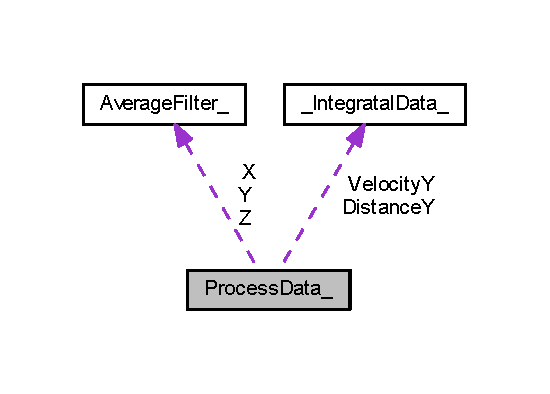
\includegraphics[width=264pt]{struct_process_data____coll__graph}
\end{center}
\end{figure}
\subsection*{Data Fields}
\begin{DoxyCompactItemize}
\item 
float \mbox{\hyperlink{struct_process_data___a92338f7520578c54d577bf8dd193186c}{Accelerometer\+\_\+X}}
\item 
float \mbox{\hyperlink{struct_process_data___a0630656d6ec984a6917aba7d0617d87b}{calibrationY}}
\item 
float \mbox{\hyperlink{struct_process_data___a1a3f3515022e230ceaf847b59f45d244}{Accelerometer\+\_\+Y}}
\item 
float \mbox{\hyperlink{struct_process_data___afe6d67e3ee7305c3f5fc242162aa13b2}{Accelerometer\+\_\+Z}}
\item 
float \mbox{\hyperlink{struct_process_data___ae36f07f578d32279404707bc16db33db}{Temp\+\_\+\+Displacement}}
\item 
\mbox{\hyperlink{filter__math__pincinato_8h_a05751bcbb0782121ff05ae3b7fc37dac}{Average\+Filter}} \mbox{\hyperlink{struct_process_data___a1dddeebb5e500ffea1704c56bad3e5de}{X}}
\item 
\mbox{\hyperlink{filter__math__pincinato_8h_a05751bcbb0782121ff05ae3b7fc37dac}{Average\+Filter}} \mbox{\hyperlink{struct_process_data___a999e007debe5468384855f5109e979c8}{Y}}
\item 
float \mbox{\hyperlink{struct_process_data___a19b2872341d3b0c7cf6c7b5744680b48}{DataY}} \mbox{[}\mbox{\hyperlink{interface___a_c_c_e_l__pincinato_8h_af704f1402c3ac42c867882facf46fc66}{filter\+Item\+Count}}\mbox{]}
\item 
\mbox{\hyperlink{filter__math__pincinato_8h_a05751bcbb0782121ff05ae3b7fc37dac}{Average\+Filter}} \mbox{\hyperlink{struct_process_data___adcecb30f0d09efbdf979b7162fd73a59}{Z}}
\item 
\mbox{\hyperlink{filter__math__pincinato_8h_a614628710e855bdeb4949c83265e87e6}{Integration\+Data}} \mbox{\hyperlink{struct_process_data___ac8287aab78b8f4b55b7284b8b9d2d6eb}{VelocityY}}
\item 
float \mbox{\hyperlink{struct_process_data___a4fa27dc016870a216daf63ba65059a0b}{Data\+VelocityY}} \mbox{[}\mbox{\hyperlink{interface___a_c_c_e_l__pincinato_8h_aeee7ebe36cd3653f48821e6d0da7029d}{integration\+Length}}\mbox{]}
\item 
\mbox{\hyperlink{filter__math__pincinato_8h_a614628710e855bdeb4949c83265e87e6}{Integration\+Data}} \mbox{\hyperlink{struct_process_data___a9505c01279b7b5fe0e636e607ad4d63d}{DistanceY}}
\item 
float \mbox{\hyperlink{struct_process_data___ac4266b27959dc8e308a8741c9913f93c}{Data\+DistanceY}} \mbox{[}\mbox{\hyperlink{interface___a_c_c_e_l__pincinato_8h_aeee7ebe36cd3653f48821e6d0da7029d}{integration\+Length}}\mbox{]}
\end{DoxyCompactItemize}


\subsection{Detailed Description}


Definition at line 38 of file interface\+\_\+\+A\+C\+C\+E\+L\+\_\+pincinato.\+h.



\subsection{Field Documentation}
\mbox{\Hypertarget{struct_process_data___a92338f7520578c54d577bf8dd193186c}\label{struct_process_data___a92338f7520578c54d577bf8dd193186c}} 
\index{Process\+Data\+\_\+@{Process\+Data\+\_\+}!Accelerometer\+\_\+X@{Accelerometer\+\_\+X}}
\index{Accelerometer\+\_\+X@{Accelerometer\+\_\+X}!Process\+Data\+\_\+@{Process\+Data\+\_\+}}
\subsubsection{\texorpdfstring{Accelerometer\+\_\+X}{Accelerometer\_X}}
{\footnotesize\ttfamily float Accelerometer\+\_\+X}



Definition at line 39 of file interface\+\_\+\+A\+C\+C\+E\+L\+\_\+pincinato.\+h.

\mbox{\Hypertarget{struct_process_data___a1a3f3515022e230ceaf847b59f45d244}\label{struct_process_data___a1a3f3515022e230ceaf847b59f45d244}} 
\index{Process\+Data\+\_\+@{Process\+Data\+\_\+}!Accelerometer\+\_\+Y@{Accelerometer\+\_\+Y}}
\index{Accelerometer\+\_\+Y@{Accelerometer\+\_\+Y}!Process\+Data\+\_\+@{Process\+Data\+\_\+}}
\subsubsection{\texorpdfstring{Accelerometer\+\_\+Y}{Accelerometer\_Y}}
{\footnotesize\ttfamily float Accelerometer\+\_\+Y}



Definition at line 41 of file interface\+\_\+\+A\+C\+C\+E\+L\+\_\+pincinato.\+h.

\mbox{\Hypertarget{struct_process_data___afe6d67e3ee7305c3f5fc242162aa13b2}\label{struct_process_data___afe6d67e3ee7305c3f5fc242162aa13b2}} 
\index{Process\+Data\+\_\+@{Process\+Data\+\_\+}!Accelerometer\+\_\+Z@{Accelerometer\+\_\+Z}}
\index{Accelerometer\+\_\+Z@{Accelerometer\+\_\+Z}!Process\+Data\+\_\+@{Process\+Data\+\_\+}}
\subsubsection{\texorpdfstring{Accelerometer\+\_\+Z}{Accelerometer\_Z}}
{\footnotesize\ttfamily float Accelerometer\+\_\+Z}



Definition at line 42 of file interface\+\_\+\+A\+C\+C\+E\+L\+\_\+pincinato.\+h.

\mbox{\Hypertarget{struct_process_data___a0630656d6ec984a6917aba7d0617d87b}\label{struct_process_data___a0630656d6ec984a6917aba7d0617d87b}} 
\index{Process\+Data\+\_\+@{Process\+Data\+\_\+}!calibrationY@{calibrationY}}
\index{calibrationY@{calibrationY}!Process\+Data\+\_\+@{Process\+Data\+\_\+}}
\subsubsection{\texorpdfstring{calibrationY}{calibrationY}}
{\footnotesize\ttfamily float calibrationY}



Definition at line 40 of file interface\+\_\+\+A\+C\+C\+E\+L\+\_\+pincinato.\+h.

\mbox{\Hypertarget{struct_process_data___ac4266b27959dc8e308a8741c9913f93c}\label{struct_process_data___ac4266b27959dc8e308a8741c9913f93c}} 
\index{Process\+Data\+\_\+@{Process\+Data\+\_\+}!Data\+DistanceY@{Data\+DistanceY}}
\index{Data\+DistanceY@{Data\+DistanceY}!Process\+Data\+\_\+@{Process\+Data\+\_\+}}
\subsubsection{\texorpdfstring{Data\+DistanceY}{DataDistanceY}}
{\footnotesize\ttfamily float Data\+DistanceY\mbox{[}\mbox{\hyperlink{interface___a_c_c_e_l__pincinato_8h_aeee7ebe36cd3653f48821e6d0da7029d}{integration\+Length}}\mbox{]}}



Definition at line 51 of file interface\+\_\+\+A\+C\+C\+E\+L\+\_\+pincinato.\+h.

\mbox{\Hypertarget{struct_process_data___a4fa27dc016870a216daf63ba65059a0b}\label{struct_process_data___a4fa27dc016870a216daf63ba65059a0b}} 
\index{Process\+Data\+\_\+@{Process\+Data\+\_\+}!Data\+VelocityY@{Data\+VelocityY}}
\index{Data\+VelocityY@{Data\+VelocityY}!Process\+Data\+\_\+@{Process\+Data\+\_\+}}
\subsubsection{\texorpdfstring{Data\+VelocityY}{DataVelocityY}}
{\footnotesize\ttfamily float Data\+VelocityY\mbox{[}\mbox{\hyperlink{interface___a_c_c_e_l__pincinato_8h_aeee7ebe36cd3653f48821e6d0da7029d}{integration\+Length}}\mbox{]}}



Definition at line 49 of file interface\+\_\+\+A\+C\+C\+E\+L\+\_\+pincinato.\+h.

\mbox{\Hypertarget{struct_process_data___a19b2872341d3b0c7cf6c7b5744680b48}\label{struct_process_data___a19b2872341d3b0c7cf6c7b5744680b48}} 
\index{Process\+Data\+\_\+@{Process\+Data\+\_\+}!DataY@{DataY}}
\index{DataY@{DataY}!Process\+Data\+\_\+@{Process\+Data\+\_\+}}
\subsubsection{\texorpdfstring{DataY}{DataY}}
{\footnotesize\ttfamily float DataY\mbox{[}\mbox{\hyperlink{interface___a_c_c_e_l__pincinato_8h_af704f1402c3ac42c867882facf46fc66}{filter\+Item\+Count}}\mbox{]}}



Definition at line 46 of file interface\+\_\+\+A\+C\+C\+E\+L\+\_\+pincinato.\+h.

\mbox{\Hypertarget{struct_process_data___a9505c01279b7b5fe0e636e607ad4d63d}\label{struct_process_data___a9505c01279b7b5fe0e636e607ad4d63d}} 
\index{Process\+Data\+\_\+@{Process\+Data\+\_\+}!DistanceY@{DistanceY}}
\index{DistanceY@{DistanceY}!Process\+Data\+\_\+@{Process\+Data\+\_\+}}
\subsubsection{\texorpdfstring{DistanceY}{DistanceY}}
{\footnotesize\ttfamily \mbox{\hyperlink{filter__math__pincinato_8h_a614628710e855bdeb4949c83265e87e6}{Integration\+Data}} DistanceY}



Definition at line 50 of file interface\+\_\+\+A\+C\+C\+E\+L\+\_\+pincinato.\+h.

\mbox{\Hypertarget{struct_process_data___ae36f07f578d32279404707bc16db33db}\label{struct_process_data___ae36f07f578d32279404707bc16db33db}} 
\index{Process\+Data\+\_\+@{Process\+Data\+\_\+}!Temp\+\_\+\+Displacement@{Temp\+\_\+\+Displacement}}
\index{Temp\+\_\+\+Displacement@{Temp\+\_\+\+Displacement}!Process\+Data\+\_\+@{Process\+Data\+\_\+}}
\subsubsection{\texorpdfstring{Temp\+\_\+\+Displacement}{Temp\_Displacement}}
{\footnotesize\ttfamily float Temp\+\_\+\+Displacement}



Definition at line 43 of file interface\+\_\+\+A\+C\+C\+E\+L\+\_\+pincinato.\+h.

\mbox{\Hypertarget{struct_process_data___ac8287aab78b8f4b55b7284b8b9d2d6eb}\label{struct_process_data___ac8287aab78b8f4b55b7284b8b9d2d6eb}} 
\index{Process\+Data\+\_\+@{Process\+Data\+\_\+}!VelocityY@{VelocityY}}
\index{VelocityY@{VelocityY}!Process\+Data\+\_\+@{Process\+Data\+\_\+}}
\subsubsection{\texorpdfstring{VelocityY}{VelocityY}}
{\footnotesize\ttfamily \mbox{\hyperlink{filter__math__pincinato_8h_a614628710e855bdeb4949c83265e87e6}{Integration\+Data}} VelocityY}



Definition at line 48 of file interface\+\_\+\+A\+C\+C\+E\+L\+\_\+pincinato.\+h.

\mbox{\Hypertarget{struct_process_data___a1dddeebb5e500ffea1704c56bad3e5de}\label{struct_process_data___a1dddeebb5e500ffea1704c56bad3e5de}} 
\index{Process\+Data\+\_\+@{Process\+Data\+\_\+}!X@{X}}
\index{X@{X}!Process\+Data\+\_\+@{Process\+Data\+\_\+}}
\subsubsection{\texorpdfstring{X}{X}}
{\footnotesize\ttfamily \mbox{\hyperlink{filter__math__pincinato_8h_a05751bcbb0782121ff05ae3b7fc37dac}{Average\+Filter}} X}



Definition at line 44 of file interface\+\_\+\+A\+C\+C\+E\+L\+\_\+pincinato.\+h.

\mbox{\Hypertarget{struct_process_data___a999e007debe5468384855f5109e979c8}\label{struct_process_data___a999e007debe5468384855f5109e979c8}} 
\index{Process\+Data\+\_\+@{Process\+Data\+\_\+}!Y@{Y}}
\index{Y@{Y}!Process\+Data\+\_\+@{Process\+Data\+\_\+}}
\subsubsection{\texorpdfstring{Y}{Y}}
{\footnotesize\ttfamily \mbox{\hyperlink{filter__math__pincinato_8h_a05751bcbb0782121ff05ae3b7fc37dac}{Average\+Filter}} Y}



Definition at line 45 of file interface\+\_\+\+A\+C\+C\+E\+L\+\_\+pincinato.\+h.

\mbox{\Hypertarget{struct_process_data___adcecb30f0d09efbdf979b7162fd73a59}\label{struct_process_data___adcecb30f0d09efbdf979b7162fd73a59}} 
\index{Process\+Data\+\_\+@{Process\+Data\+\_\+}!Z@{Z}}
\index{Z@{Z}!Process\+Data\+\_\+@{Process\+Data\+\_\+}}
\subsubsection{\texorpdfstring{Z}{Z}}
{\footnotesize\ttfamily \mbox{\hyperlink{filter__math__pincinato_8h_a05751bcbb0782121ff05ae3b7fc37dac}{Average\+Filter}} Z}



Definition at line 47 of file interface\+\_\+\+A\+C\+C\+E\+L\+\_\+pincinato.\+h.



The documentation for this struct was generated from the following file\+:\begin{DoxyCompactItemize}
\item 
C\+:/\+Users/\+T\+H\+P/\+Desktop/\+Unibern/2018\+\_\+02/\+Subjects/\+Programming\+\_\+\+Microcontroller/\+Paeks/samples/\+My\+\_\+\+Project/\+Library/\+Library/inc/\mbox{\hyperlink{interface___a_c_c_e_l__pincinato_8h}{interface\+\_\+\+A\+C\+C\+E\+L\+\_\+pincinato.\+h}}\end{DoxyCompactItemize}

\hypertarget{struct_process_data____}{}\section{Process\+Data\+\_\+\+\_\+ Struct Reference}
\label{struct_process_data____}\index{Process\+Data\+\_\+\+\_\+@{Process\+Data\+\_\+\+\_\+}}


{\ttfamily \#include $<$interface\+\_\+\+A\+D\+C\+\_\+pincinato.\+h$>$}



Collaboration diagram for Process\+Data\+\_\+\+\_\+\+:\nopagebreak
\begin{figure}[H]
\begin{center}
\leavevmode
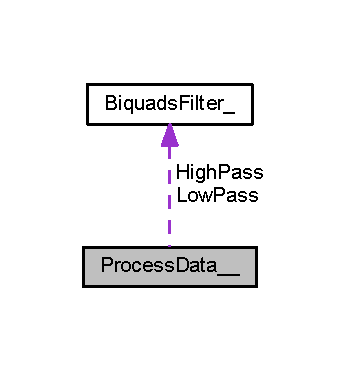
\includegraphics[width=168pt]{struct_process_data______coll__graph}
\end{center}
\end{figure}
\subsection*{Data Fields}
\begin{DoxyCompactItemize}
\item 
\mbox{\hyperlink{filter__math__pincinato_8h_a431282902bc1cfeb168d1acf574331bb}{Biquads\+Filter}} \mbox{\hyperlink{struct_process_data_____af13bc04872597bbd10728a615e35f0a8}{High\+Pass}}
\item 
float \mbox{\hyperlink{struct_process_data_____a4c0a993848fc70e7ee3eb5e55bf88fa2}{Highbuf}} \mbox{[}\mbox{\hyperlink{interface___a_d_c__pincinato_8h_a2ddc9b0b00b7c686d5208fc298aeadb2}{A\+D\+C\+B\+U\+F\+F\+E\+R\+L\+E\+N\+G\+TH}}\mbox{]}
\item 
\mbox{\hyperlink{filter__math__pincinato_8h_a431282902bc1cfeb168d1acf574331bb}{Biquads\+Filter}} \mbox{\hyperlink{struct_process_data_____aed3be52a787eac3e0d0981dd8c2bb8a0}{Low\+Pass}}
\item 
float \mbox{\hyperlink{struct_process_data_____a5e4aeedf9f04a1d8ee5bad2b8e0bf8af}{Lowbuf}} \mbox{[}\mbox{\hyperlink{interface___a_d_c__pincinato_8h_a2ddc9b0b00b7c686d5208fc298aeadb2}{A\+D\+C\+B\+U\+F\+F\+E\+R\+L\+E\+N\+G\+TH}}\mbox{]}
\end{DoxyCompactItemize}


\subsection{Detailed Description}


Definition at line 27 of file interface\+\_\+\+A\+D\+C\+\_\+pincinato.\+h.



\subsection{Field Documentation}
\mbox{\Hypertarget{struct_process_data_____a4c0a993848fc70e7ee3eb5e55bf88fa2}\label{struct_process_data_____a4c0a993848fc70e7ee3eb5e55bf88fa2}} 
\index{Process\+Data\+\_\+\+\_\+@{Process\+Data\+\_\+\+\_\+}!Highbuf@{Highbuf}}
\index{Highbuf@{Highbuf}!Process\+Data\+\_\+\+\_\+@{Process\+Data\+\_\+\+\_\+}}
\subsubsection{\texorpdfstring{Highbuf}{Highbuf}}
{\footnotesize\ttfamily float Highbuf\mbox{[}\mbox{\hyperlink{interface___a_d_c__pincinato_8h_a2ddc9b0b00b7c686d5208fc298aeadb2}{A\+D\+C\+B\+U\+F\+F\+E\+R\+L\+E\+N\+G\+TH}}\mbox{]}}



Definition at line 29 of file interface\+\_\+\+A\+D\+C\+\_\+pincinato.\+h.

\mbox{\Hypertarget{struct_process_data_____af13bc04872597bbd10728a615e35f0a8}\label{struct_process_data_____af13bc04872597bbd10728a615e35f0a8}} 
\index{Process\+Data\+\_\+\+\_\+@{Process\+Data\+\_\+\+\_\+}!High\+Pass@{High\+Pass}}
\index{High\+Pass@{High\+Pass}!Process\+Data\+\_\+\+\_\+@{Process\+Data\+\_\+\+\_\+}}
\subsubsection{\texorpdfstring{High\+Pass}{HighPass}}
{\footnotesize\ttfamily \mbox{\hyperlink{filter__math__pincinato_8h_a431282902bc1cfeb168d1acf574331bb}{Biquads\+Filter}} High\+Pass}



Definition at line 28 of file interface\+\_\+\+A\+D\+C\+\_\+pincinato.\+h.

\mbox{\Hypertarget{struct_process_data_____a5e4aeedf9f04a1d8ee5bad2b8e0bf8af}\label{struct_process_data_____a5e4aeedf9f04a1d8ee5bad2b8e0bf8af}} 
\index{Process\+Data\+\_\+\+\_\+@{Process\+Data\+\_\+\+\_\+}!Lowbuf@{Lowbuf}}
\index{Lowbuf@{Lowbuf}!Process\+Data\+\_\+\+\_\+@{Process\+Data\+\_\+\+\_\+}}
\subsubsection{\texorpdfstring{Lowbuf}{Lowbuf}}
{\footnotesize\ttfamily float Lowbuf\mbox{[}\mbox{\hyperlink{interface___a_d_c__pincinato_8h_a2ddc9b0b00b7c686d5208fc298aeadb2}{A\+D\+C\+B\+U\+F\+F\+E\+R\+L\+E\+N\+G\+TH}}\mbox{]}}



Definition at line 31 of file interface\+\_\+\+A\+D\+C\+\_\+pincinato.\+h.

\mbox{\Hypertarget{struct_process_data_____aed3be52a787eac3e0d0981dd8c2bb8a0}\label{struct_process_data_____aed3be52a787eac3e0d0981dd8c2bb8a0}} 
\index{Process\+Data\+\_\+\+\_\+@{Process\+Data\+\_\+\+\_\+}!Low\+Pass@{Low\+Pass}}
\index{Low\+Pass@{Low\+Pass}!Process\+Data\+\_\+\+\_\+@{Process\+Data\+\_\+\+\_\+}}
\subsubsection{\texorpdfstring{Low\+Pass}{LowPass}}
{\footnotesize\ttfamily \mbox{\hyperlink{filter__math__pincinato_8h_a431282902bc1cfeb168d1acf574331bb}{Biquads\+Filter}} Low\+Pass}



Definition at line 30 of file interface\+\_\+\+A\+D\+C\+\_\+pincinato.\+h.



The documentation for this struct was generated from the following file\+:\begin{DoxyCompactItemize}
\item 
Library/\+Library/inc/\mbox{\hyperlink{interface___a_d_c__pincinato_8h}{interface\+\_\+\+A\+D\+C\+\_\+pincinato.\+h}}\end{DoxyCompactItemize}

\hypertarget{struct_process_data______}{}\section{Process\+Data\+\_\+\+\_\+\+\_\+ Struct Reference}
\label{struct_process_data______}\index{Process\+Data\+\_\+\+\_\+\+\_\+@{Process\+Data\+\_\+\+\_\+\+\_\+}}


{\ttfamily \#include $<$interface\+\_\+\+E\+C\+G\+\_\+pincinato.\+h$>$}



Collaboration diagram for Process\+Data\+\_\+\+\_\+\+\_\+\+:\nopagebreak
\begin{figure}[H]
\begin{center}
\leavevmode
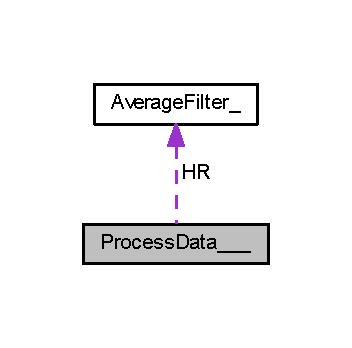
\includegraphics[width=169pt]{struct_process_data________coll__graph}
\end{center}
\end{figure}
\subsection*{Data Fields}
\begin{DoxyCompactItemize}
\item 
\mbox{\hyperlink{filter__math__pincinato_8h_a05751bcbb0782121ff05ae3b7fc37dac}{Average\+Filter}} \mbox{\hyperlink{struct_process_data_______afa7d4c3f6f59fcc62e758b829d298569}{HR}}
\item 
float \mbox{\hyperlink{struct_process_data_______aa85aa87ff25601cf758c39958653d60a}{H\+R\+\_\+threshold}}
\item 
float \mbox{\hyperlink{struct_process_data_______abe41d3213d4f1e10d1ce88c78db23a22}{H\+Rbuf}} \mbox{[}\mbox{\hyperlink{interface___e_c_g__pincinato_8h_aa57c4fd3ea06cc9a9c4e8ecda369ed58}{low\+Filter\+Item\+Count}}\mbox{]}
\end{DoxyCompactItemize}


\subsection{Detailed Description}


Definition at line 19 of file interface\+\_\+\+E\+C\+G\+\_\+pincinato.\+h.



\subsection{Field Documentation}
\mbox{\Hypertarget{struct_process_data_______afa7d4c3f6f59fcc62e758b829d298569}\label{struct_process_data_______afa7d4c3f6f59fcc62e758b829d298569}} 
\index{Process\+Data\+\_\+\+\_\+\+\_\+@{Process\+Data\+\_\+\+\_\+\+\_\+}!HR@{HR}}
\index{HR@{HR}!Process\+Data\+\_\+\+\_\+\+\_\+@{Process\+Data\+\_\+\+\_\+\+\_\+}}
\subsubsection{\texorpdfstring{HR}{HR}}
{\footnotesize\ttfamily \mbox{\hyperlink{filter__math__pincinato_8h_a05751bcbb0782121ff05ae3b7fc37dac}{Average\+Filter}} HR}



Definition at line 20 of file interface\+\_\+\+E\+C\+G\+\_\+pincinato.\+h.

\mbox{\Hypertarget{struct_process_data_______aa85aa87ff25601cf758c39958653d60a}\label{struct_process_data_______aa85aa87ff25601cf758c39958653d60a}} 
\index{Process\+Data\+\_\+\+\_\+\+\_\+@{Process\+Data\+\_\+\+\_\+\+\_\+}!H\+R\+\_\+threshold@{H\+R\+\_\+threshold}}
\index{H\+R\+\_\+threshold@{H\+R\+\_\+threshold}!Process\+Data\+\_\+\+\_\+\+\_\+@{Process\+Data\+\_\+\+\_\+\+\_\+}}
\subsubsection{\texorpdfstring{H\+R\+\_\+threshold}{HR\_threshold}}
{\footnotesize\ttfamily float H\+R\+\_\+threshold}



Definition at line 21 of file interface\+\_\+\+E\+C\+G\+\_\+pincinato.\+h.

\mbox{\Hypertarget{struct_process_data_______abe41d3213d4f1e10d1ce88c78db23a22}\label{struct_process_data_______abe41d3213d4f1e10d1ce88c78db23a22}} 
\index{Process\+Data\+\_\+\+\_\+\+\_\+@{Process\+Data\+\_\+\+\_\+\+\_\+}!H\+Rbuf@{H\+Rbuf}}
\index{H\+Rbuf@{H\+Rbuf}!Process\+Data\+\_\+\+\_\+\+\_\+@{Process\+Data\+\_\+\+\_\+\+\_\+}}
\subsubsection{\texorpdfstring{H\+Rbuf}{HRbuf}}
{\footnotesize\ttfamily float H\+Rbuf\mbox{[}\mbox{\hyperlink{interface___e_c_g__pincinato_8h_aa57c4fd3ea06cc9a9c4e8ecda369ed58}{low\+Filter\+Item\+Count}}\mbox{]}}



Definition at line 22 of file interface\+\_\+\+E\+C\+G\+\_\+pincinato.\+h.



The documentation for this struct was generated from the following file\+:\begin{DoxyCompactItemize}
\item 
Library/\+Library/inc/\mbox{\hyperlink{interface___e_c_g__pincinato_8h}{interface\+\_\+\+E\+C\+G\+\_\+pincinato.\+h}}\end{DoxyCompactItemize}

\hypertarget{struct_table}{}\section{Table Struct Reference}
\label{struct_table}\index{Table@{Table}}


{\ttfamily \#include $<$structs\+\_\+pincinato.\+h$>$}

\subsection*{Data Fields}
\begin{DoxyCompactItemize}
\item 
uint32\+\_\+t \mbox{\hyperlink{struct_table_a083b719ad6c79f4ae24629ff524568c5}{High\+\_\+\+Heart\+Rate}}
\item 
uint32\+\_\+t \mbox{\hyperlink{struct_table_a2639bf590ecf1e2847a7cc426eb9286b}{Normal\+\_\+\+Heart\+Rate}}
\item 
uint32\+\_\+t \mbox{\hyperlink{struct_table_abee6357a367856ae631545d1499ae7cd}{Low\+\_\+\+Heart\+Rate}}
\item 
bool \mbox{\hyperlink{struct_table_a29b7719b9fe37705659ac979eb31ab54}{Has\+Been\+Edited}}
\end{DoxyCompactItemize}


\subsection{Detailed Description}


Definition at line 12 of file structs\+\_\+pincinato.\+h.



\subsection{Field Documentation}
\mbox{\Hypertarget{struct_table_a29b7719b9fe37705659ac979eb31ab54}\label{struct_table_a29b7719b9fe37705659ac979eb31ab54}} 
\index{Table@{Table}!Has\+Been\+Edited@{Has\+Been\+Edited}}
\index{Has\+Been\+Edited@{Has\+Been\+Edited}!Table@{Table}}
\subsubsection{\texorpdfstring{Has\+Been\+Edited}{HasBeenEdited}}
{\footnotesize\ttfamily bool Has\+Been\+Edited}



Definition at line 17 of file structs\+\_\+pincinato.\+h.

\mbox{\Hypertarget{struct_table_a083b719ad6c79f4ae24629ff524568c5}\label{struct_table_a083b719ad6c79f4ae24629ff524568c5}} 
\index{Table@{Table}!High\+\_\+\+Heart\+Rate@{High\+\_\+\+Heart\+Rate}}
\index{High\+\_\+\+Heart\+Rate@{High\+\_\+\+Heart\+Rate}!Table@{Table}}
\subsubsection{\texorpdfstring{High\+\_\+\+Heart\+Rate}{High\_HeartRate}}
{\footnotesize\ttfamily uint32\+\_\+t High\+\_\+\+Heart\+Rate}



Definition at line 14 of file structs\+\_\+pincinato.\+h.

\mbox{\Hypertarget{struct_table_abee6357a367856ae631545d1499ae7cd}\label{struct_table_abee6357a367856ae631545d1499ae7cd}} 
\index{Table@{Table}!Low\+\_\+\+Heart\+Rate@{Low\+\_\+\+Heart\+Rate}}
\index{Low\+\_\+\+Heart\+Rate@{Low\+\_\+\+Heart\+Rate}!Table@{Table}}
\subsubsection{\texorpdfstring{Low\+\_\+\+Heart\+Rate}{Low\_HeartRate}}
{\footnotesize\ttfamily uint32\+\_\+t Low\+\_\+\+Heart\+Rate}



Definition at line 16 of file structs\+\_\+pincinato.\+h.

\mbox{\Hypertarget{struct_table_a2639bf590ecf1e2847a7cc426eb9286b}\label{struct_table_a2639bf590ecf1e2847a7cc426eb9286b}} 
\index{Table@{Table}!Normal\+\_\+\+Heart\+Rate@{Normal\+\_\+\+Heart\+Rate}}
\index{Normal\+\_\+\+Heart\+Rate@{Normal\+\_\+\+Heart\+Rate}!Table@{Table}}
\subsubsection{\texorpdfstring{Normal\+\_\+\+Heart\+Rate}{Normal\_HeartRate}}
{\footnotesize\ttfamily uint32\+\_\+t Normal\+\_\+\+Heart\+Rate}



Definition at line 15 of file structs\+\_\+pincinato.\+h.



The documentation for this struct was generated from the following file\+:\begin{DoxyCompactItemize}
\item 
C\+:/\+Users/\+T\+H\+P/\+Desktop/\+Unibern/2018\+\_\+02/\+Subjects/\+Programming\+\_\+\+Microcontroller/\+Paeks/samples/\+My\+\_\+\+Project/\+Library/\+Library/inc/\mbox{\hyperlink{structs__pincinato_8h}{structs\+\_\+pincinato.\+h}}\end{DoxyCompactItemize}

\hypertarget{uniontmc260___chopper_control_register__}{}\section{tmc260\+\_\+\+Chopper\+Control\+Register\+\_\+ Union Reference}
\label{uniontmc260___chopper_control_register__}\index{tmc260\+\_\+\+Chopper\+Control\+Register\+\_\+@{tmc260\+\_\+\+Chopper\+Control\+Register\+\_\+}}


{\ttfamily \#include $<$tmc260\+\_\+driver.\+h$>$}

\subsection*{Data Fields}
\begin{DoxyCompactItemize}
\item 
\mbox{\hyperlink{tmc260__driver_8h_a280b01a3b5bb4294fcee278b00c030d6}{Register}} \mbox{\hyperlink{uniontmc260___chopper_control_register___a445b72174063a88455cd86c22d77d03f}{bytes}}
\item 
\begin{tabbing}
xx\=xx\=xx\=xx\=xx\=xx\=xx\=xx\=xx\=\kill
struct \{\\
\>uint32\_t \mbox{\hyperlink{uniontmc260___chopper_control_register___ac823d0b0cbdcb4f8b362cdba9d912ee2}{offTimeOrMosfetDisable}}: 4\\
\>uint32\_t \mbox{\hyperlink{uniontmc260___chopper_control_register___ac2d01ebf0d937be909c0f2daf54d3b6a}{hysteresisStartOrFastDecayTime}}: 3\\
\>uint32\_t \mbox{\hyperlink{uniontmc260___chopper_control_register___a6299a53ed5b8d4d016816293d2cafce2}{hysteresisEndOrSineWaveOffset}}: 4\\
\>uint32\_t \mbox{\hyperlink{uniontmc260___chopper_control_register___ac4ee7b51371e5f076bf691c71e679d2f}{hysteresisDecrementIntervalOrFastDecayMode}}: 2\\
\>uint32\_t \mbox{\hyperlink{uniontmc260___chopper_control_register___a1cedcadd3f5e38a49f24d07c4cb75886}{randomToffTime}}: 1\\
\>uint32\_t \mbox{\hyperlink{uniontmc260___chopper_control_register___a00949da3a97cb42796ef2161cd0817bc}{chopperMode}}: 1\\
\>uint32\_t \mbox{\hyperlink{uniontmc260___chopper_control_register___af5b56d8dbfe1afbaef2fa2b6703bfa6d}{blankingTime}}: 2\\
\>uint32\_t \mbox{\hyperlink{uniontmc260___chopper_control_register___a8e58d0701295971bc3d890f5107f8aa5}{registerAdressBit\_1}}: 1\\
\>uint32\_t \mbox{\hyperlink{uniontmc260___chopper_control_register___abd6d1c957737511340b85f5c2d61f9ab}{registerAdressBit\_2}}: 1\\
\>uint32\_t \mbox{\hyperlink{uniontmc260___chopper_control_register___a3da0387ab629039b91d051ab328910f0}{registerAdressBit\_3}}: 1\\
\>uint32\_t \mbox{\hyperlink{uniontmc260___chopper_control_register___a3e57c2ef1c3ffb36722f000cc1156824}{\_\_pad0\_\_}}: 4\\
\} \mbox{\hyperlink{uniontmc260___chopper_control_register___a4bff58b2954e71c724912bb179e34070}{bits}}\\

\end{tabbing}\end{DoxyCompactItemize}


\subsection{Detailed Description}
Union to represent the chopper control register (C\+H\+O\+P\+C\+O\+NF) of a tmc260 device as bitfield 

Definition at line 57 of file tmc260\+\_\+driver.\+h.



\subsection{Field Documentation}
\mbox{\Hypertarget{uniontmc260___chopper_control_register___a3e57c2ef1c3ffb36722f000cc1156824}\label{uniontmc260___chopper_control_register___a3e57c2ef1c3ffb36722f000cc1156824}} 
\index{tmc260\+\_\+\+Chopper\+Control\+Register\+\_\+@{tmc260\+\_\+\+Chopper\+Control\+Register\+\_\+}!\+\_\+\+\_\+pad0\+\_\+\+\_\+@{\+\_\+\+\_\+pad0\+\_\+\+\_\+}}
\index{\+\_\+\+\_\+pad0\+\_\+\+\_\+@{\+\_\+\+\_\+pad0\+\_\+\+\_\+}!tmc260\+\_\+\+Chopper\+Control\+Register\+\_\+@{tmc260\+\_\+\+Chopper\+Control\+Register\+\_\+}}
\subsubsection{\texorpdfstring{\+\_\+\+\_\+pad0\+\_\+\+\_\+}{\_\_pad0\_\_}}
{\footnotesize\ttfamily uint32\+\_\+t \+\_\+\+\_\+pad0\+\_\+\+\_\+}



Definition at line 70 of file tmc260\+\_\+driver.\+h.

\mbox{\Hypertarget{uniontmc260___chopper_control_register___a4bff58b2954e71c724912bb179e34070}\label{uniontmc260___chopper_control_register___a4bff58b2954e71c724912bb179e34070}} 
\index{tmc260\+\_\+\+Chopper\+Control\+Register\+\_\+@{tmc260\+\_\+\+Chopper\+Control\+Register\+\_\+}!bits@{bits}}
\index{bits@{bits}!tmc260\+\_\+\+Chopper\+Control\+Register\+\_\+@{tmc260\+\_\+\+Chopper\+Control\+Register\+\_\+}}
\subsubsection{\texorpdfstring{bits}{bits}}
{\footnotesize\ttfamily struct \{ ... \}  bits}

\mbox{\Hypertarget{uniontmc260___chopper_control_register___af5b56d8dbfe1afbaef2fa2b6703bfa6d}\label{uniontmc260___chopper_control_register___af5b56d8dbfe1afbaef2fa2b6703bfa6d}} 
\index{tmc260\+\_\+\+Chopper\+Control\+Register\+\_\+@{tmc260\+\_\+\+Chopper\+Control\+Register\+\_\+}!blanking\+Time@{blanking\+Time}}
\index{blanking\+Time@{blanking\+Time}!tmc260\+\_\+\+Chopper\+Control\+Register\+\_\+@{tmc260\+\_\+\+Chopper\+Control\+Register\+\_\+}}
\subsubsection{\texorpdfstring{blanking\+Time}{blankingTime}}
{\footnotesize\ttfamily uint32\+\_\+t blanking\+Time}



Definition at line 66 of file tmc260\+\_\+driver.\+h.

\mbox{\Hypertarget{uniontmc260___chopper_control_register___a445b72174063a88455cd86c22d77d03f}\label{uniontmc260___chopper_control_register___a445b72174063a88455cd86c22d77d03f}} 
\index{tmc260\+\_\+\+Chopper\+Control\+Register\+\_\+@{tmc260\+\_\+\+Chopper\+Control\+Register\+\_\+}!bytes@{bytes}}
\index{bytes@{bytes}!tmc260\+\_\+\+Chopper\+Control\+Register\+\_\+@{tmc260\+\_\+\+Chopper\+Control\+Register\+\_\+}}
\subsubsection{\texorpdfstring{bytes}{bytes}}
{\footnotesize\ttfamily \mbox{\hyperlink{tmc260__driver_8h_a280b01a3b5bb4294fcee278b00c030d6}{Register}} bytes}



Definition at line 58 of file tmc260\+\_\+driver.\+h.

\mbox{\Hypertarget{uniontmc260___chopper_control_register___a00949da3a97cb42796ef2161cd0817bc}\label{uniontmc260___chopper_control_register___a00949da3a97cb42796ef2161cd0817bc}} 
\index{tmc260\+\_\+\+Chopper\+Control\+Register\+\_\+@{tmc260\+\_\+\+Chopper\+Control\+Register\+\_\+}!chopper\+Mode@{chopper\+Mode}}
\index{chopper\+Mode@{chopper\+Mode}!tmc260\+\_\+\+Chopper\+Control\+Register\+\_\+@{tmc260\+\_\+\+Chopper\+Control\+Register\+\_\+}}
\subsubsection{\texorpdfstring{chopper\+Mode}{chopperMode}}
{\footnotesize\ttfamily uint32\+\_\+t chopper\+Mode}



Definition at line 65 of file tmc260\+\_\+driver.\+h.

\mbox{\Hypertarget{uniontmc260___chopper_control_register___ac4ee7b51371e5f076bf691c71e679d2f}\label{uniontmc260___chopper_control_register___ac4ee7b51371e5f076bf691c71e679d2f}} 
\index{tmc260\+\_\+\+Chopper\+Control\+Register\+\_\+@{tmc260\+\_\+\+Chopper\+Control\+Register\+\_\+}!hysteresis\+Decrement\+Interval\+Or\+Fast\+Decay\+Mode@{hysteresis\+Decrement\+Interval\+Or\+Fast\+Decay\+Mode}}
\index{hysteresis\+Decrement\+Interval\+Or\+Fast\+Decay\+Mode@{hysteresis\+Decrement\+Interval\+Or\+Fast\+Decay\+Mode}!tmc260\+\_\+\+Chopper\+Control\+Register\+\_\+@{tmc260\+\_\+\+Chopper\+Control\+Register\+\_\+}}
\subsubsection{\texorpdfstring{hysteresis\+Decrement\+Interval\+Or\+Fast\+Decay\+Mode}{hysteresisDecrementIntervalOrFastDecayMode}}
{\footnotesize\ttfamily uint32\+\_\+t hysteresis\+Decrement\+Interval\+Or\+Fast\+Decay\+Mode}



Definition at line 63 of file tmc260\+\_\+driver.\+h.

\mbox{\Hypertarget{uniontmc260___chopper_control_register___a6299a53ed5b8d4d016816293d2cafce2}\label{uniontmc260___chopper_control_register___a6299a53ed5b8d4d016816293d2cafce2}} 
\index{tmc260\+\_\+\+Chopper\+Control\+Register\+\_\+@{tmc260\+\_\+\+Chopper\+Control\+Register\+\_\+}!hysteresis\+End\+Or\+Sine\+Wave\+Offset@{hysteresis\+End\+Or\+Sine\+Wave\+Offset}}
\index{hysteresis\+End\+Or\+Sine\+Wave\+Offset@{hysteresis\+End\+Or\+Sine\+Wave\+Offset}!tmc260\+\_\+\+Chopper\+Control\+Register\+\_\+@{tmc260\+\_\+\+Chopper\+Control\+Register\+\_\+}}
\subsubsection{\texorpdfstring{hysteresis\+End\+Or\+Sine\+Wave\+Offset}{hysteresisEndOrSineWaveOffset}}
{\footnotesize\ttfamily uint32\+\_\+t hysteresis\+End\+Or\+Sine\+Wave\+Offset}



Definition at line 62 of file tmc260\+\_\+driver.\+h.

\mbox{\Hypertarget{uniontmc260___chopper_control_register___ac2d01ebf0d937be909c0f2daf54d3b6a}\label{uniontmc260___chopper_control_register___ac2d01ebf0d937be909c0f2daf54d3b6a}} 
\index{tmc260\+\_\+\+Chopper\+Control\+Register\+\_\+@{tmc260\+\_\+\+Chopper\+Control\+Register\+\_\+}!hysteresis\+Start\+Or\+Fast\+Decay\+Time@{hysteresis\+Start\+Or\+Fast\+Decay\+Time}}
\index{hysteresis\+Start\+Or\+Fast\+Decay\+Time@{hysteresis\+Start\+Or\+Fast\+Decay\+Time}!tmc260\+\_\+\+Chopper\+Control\+Register\+\_\+@{tmc260\+\_\+\+Chopper\+Control\+Register\+\_\+}}
\subsubsection{\texorpdfstring{hysteresis\+Start\+Or\+Fast\+Decay\+Time}{hysteresisStartOrFastDecayTime}}
{\footnotesize\ttfamily uint32\+\_\+t hysteresis\+Start\+Or\+Fast\+Decay\+Time}



Definition at line 61 of file tmc260\+\_\+driver.\+h.

\mbox{\Hypertarget{uniontmc260___chopper_control_register___ac823d0b0cbdcb4f8b362cdba9d912ee2}\label{uniontmc260___chopper_control_register___ac823d0b0cbdcb4f8b362cdba9d912ee2}} 
\index{tmc260\+\_\+\+Chopper\+Control\+Register\+\_\+@{tmc260\+\_\+\+Chopper\+Control\+Register\+\_\+}!off\+Time\+Or\+Mosfet\+Disable@{off\+Time\+Or\+Mosfet\+Disable}}
\index{off\+Time\+Or\+Mosfet\+Disable@{off\+Time\+Or\+Mosfet\+Disable}!tmc260\+\_\+\+Chopper\+Control\+Register\+\_\+@{tmc260\+\_\+\+Chopper\+Control\+Register\+\_\+}}
\subsubsection{\texorpdfstring{off\+Time\+Or\+Mosfet\+Disable}{offTimeOrMosfetDisable}}
{\footnotesize\ttfamily uint32\+\_\+t off\+Time\+Or\+Mosfet\+Disable}



Definition at line 60 of file tmc260\+\_\+driver.\+h.

\mbox{\Hypertarget{uniontmc260___chopper_control_register___a1cedcadd3f5e38a49f24d07c4cb75886}\label{uniontmc260___chopper_control_register___a1cedcadd3f5e38a49f24d07c4cb75886}} 
\index{tmc260\+\_\+\+Chopper\+Control\+Register\+\_\+@{tmc260\+\_\+\+Chopper\+Control\+Register\+\_\+}!random\+Toff\+Time@{random\+Toff\+Time}}
\index{random\+Toff\+Time@{random\+Toff\+Time}!tmc260\+\_\+\+Chopper\+Control\+Register\+\_\+@{tmc260\+\_\+\+Chopper\+Control\+Register\+\_\+}}
\subsubsection{\texorpdfstring{random\+Toff\+Time}{randomToffTime}}
{\footnotesize\ttfamily uint32\+\_\+t random\+Toff\+Time}



Definition at line 64 of file tmc260\+\_\+driver.\+h.

\mbox{\Hypertarget{uniontmc260___chopper_control_register___a8e58d0701295971bc3d890f5107f8aa5}\label{uniontmc260___chopper_control_register___a8e58d0701295971bc3d890f5107f8aa5}} 
\index{tmc260\+\_\+\+Chopper\+Control\+Register\+\_\+@{tmc260\+\_\+\+Chopper\+Control\+Register\+\_\+}!register\+Adress\+Bit\+\_\+1@{register\+Adress\+Bit\+\_\+1}}
\index{register\+Adress\+Bit\+\_\+1@{register\+Adress\+Bit\+\_\+1}!tmc260\+\_\+\+Chopper\+Control\+Register\+\_\+@{tmc260\+\_\+\+Chopper\+Control\+Register\+\_\+}}
\subsubsection{\texorpdfstring{register\+Adress\+Bit\+\_\+1}{registerAdressBit\_1}}
{\footnotesize\ttfamily uint32\+\_\+t register\+Adress\+Bit\+\_\+1}



Definition at line 67 of file tmc260\+\_\+driver.\+h.

\mbox{\Hypertarget{uniontmc260___chopper_control_register___abd6d1c957737511340b85f5c2d61f9ab}\label{uniontmc260___chopper_control_register___abd6d1c957737511340b85f5c2d61f9ab}} 
\index{tmc260\+\_\+\+Chopper\+Control\+Register\+\_\+@{tmc260\+\_\+\+Chopper\+Control\+Register\+\_\+}!register\+Adress\+Bit\+\_\+2@{register\+Adress\+Bit\+\_\+2}}
\index{register\+Adress\+Bit\+\_\+2@{register\+Adress\+Bit\+\_\+2}!tmc260\+\_\+\+Chopper\+Control\+Register\+\_\+@{tmc260\+\_\+\+Chopper\+Control\+Register\+\_\+}}
\subsubsection{\texorpdfstring{register\+Adress\+Bit\+\_\+2}{registerAdressBit\_2}}
{\footnotesize\ttfamily uint32\+\_\+t register\+Adress\+Bit\+\_\+2}



Definition at line 68 of file tmc260\+\_\+driver.\+h.

\mbox{\Hypertarget{uniontmc260___chopper_control_register___a3da0387ab629039b91d051ab328910f0}\label{uniontmc260___chopper_control_register___a3da0387ab629039b91d051ab328910f0}} 
\index{tmc260\+\_\+\+Chopper\+Control\+Register\+\_\+@{tmc260\+\_\+\+Chopper\+Control\+Register\+\_\+}!register\+Adress\+Bit\+\_\+3@{register\+Adress\+Bit\+\_\+3}}
\index{register\+Adress\+Bit\+\_\+3@{register\+Adress\+Bit\+\_\+3}!tmc260\+\_\+\+Chopper\+Control\+Register\+\_\+@{tmc260\+\_\+\+Chopper\+Control\+Register\+\_\+}}
\subsubsection{\texorpdfstring{register\+Adress\+Bit\+\_\+3}{registerAdressBit\_3}}
{\footnotesize\ttfamily uint32\+\_\+t register\+Adress\+Bit\+\_\+3}



Definition at line 69 of file tmc260\+\_\+driver.\+h.



The documentation for this union was generated from the following file\+:\begin{DoxyCompactItemize}
\item 
Library/\+Library/inc/\mbox{\hyperlink{tmc260__driver_8h}{tmc260\+\_\+driver.\+h}}\end{DoxyCompactItemize}

\hypertarget{structtmc260___device__}{}\section{tmc260\+\_\+\+Device\+\_\+ Struct Reference}
\label{structtmc260___device__}\index{tmc260\+\_\+\+Device\+\_\+@{tmc260\+\_\+\+Device\+\_\+}}


{\ttfamily \#include $<$tmc260.\+h$>$}



Collaboration diagram for tmc260\+\_\+\+Device\+\_\+\+:\nopagebreak
\begin{figure}[H]
\begin{center}
\leavevmode
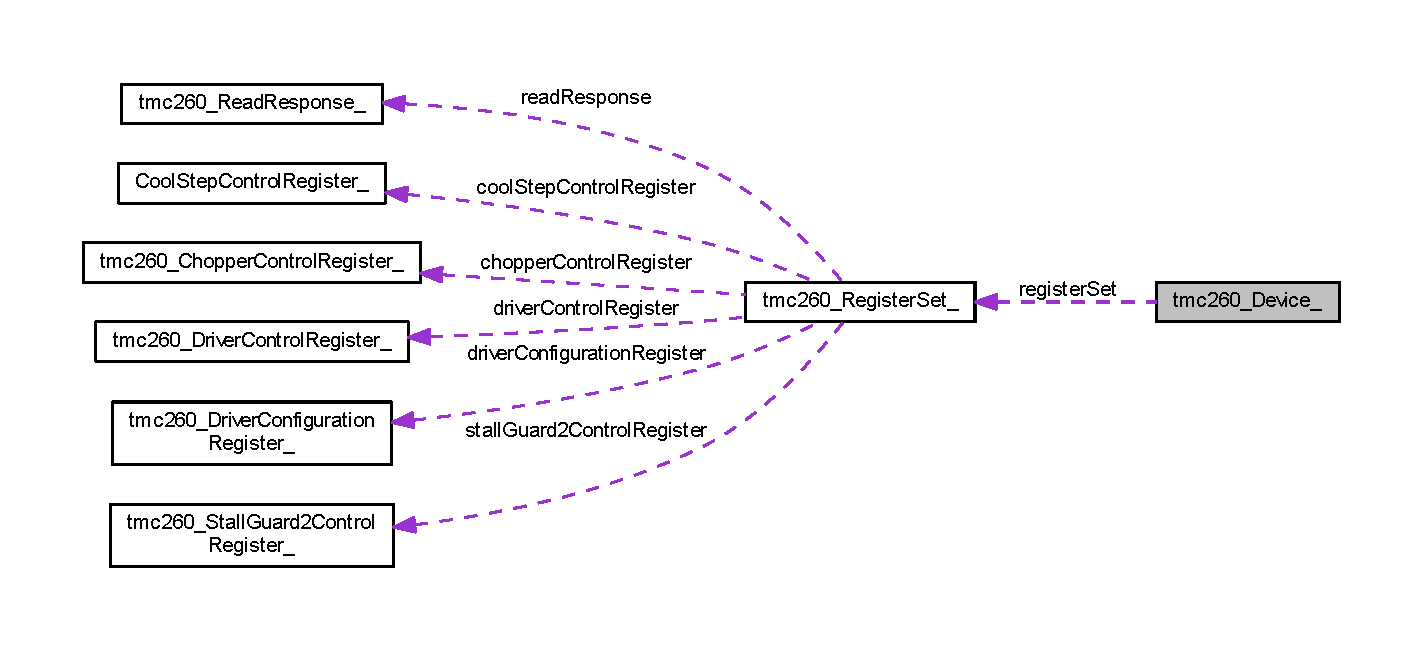
\includegraphics[width=350pt]{structtmc260___device____coll__graph}
\end{center}
\end{figure}
\subsection*{Data Fields}
\begin{DoxyCompactItemize}
\item 
\mbox{\hyperlink{tmc260_8h_a71348958a41c5e0cfdf99d907eb2ab3c}{tmc260\+\_\+\+Register\+Set}} $\ast$ \mbox{\hyperlink{structtmc260___device___a4eda80dc5e75cfc6f0e31dbf1813f418}{register\+Set}}
\item 
int8\+\_\+t($\ast$ \mbox{\hyperlink{structtmc260___device___a715a7a311876d9340872cb1d16652aeb}{set\+Parameter}} )(struct \mbox{\hyperlink{structtmc260___device__}{tmc260\+\_\+\+Device\+\_\+}} $\ast$const, \mbox{\hyperlink{tmc260_8h_af9376d3cf645591c7044d834be46c514}{tmc260\+\_\+parameter}}, uint32\+\_\+t)
\item 
int8\+\_\+t($\ast$ \mbox{\hyperlink{structtmc260___device___ac7d5bdab96761c76f99aa33aa1beb2bf}{send\+Parameter}} )(struct \mbox{\hyperlink{structtmc260___device__}{tmc260\+\_\+\+Device\+\_\+}} $\ast$const)
\end{DoxyCompactItemize}


\subsection{Detailed Description}
Structure as limited interface to the tmc260\+\_\+driver module 

Definition at line 19 of file tmc260.\+h.



\subsection{Field Documentation}
\mbox{\Hypertarget{structtmc260___device___a4eda80dc5e75cfc6f0e31dbf1813f418}\label{structtmc260___device___a4eda80dc5e75cfc6f0e31dbf1813f418}} 
\index{tmc260\+\_\+\+Device\+\_\+@{tmc260\+\_\+\+Device\+\_\+}!register\+Set@{register\+Set}}
\index{register\+Set@{register\+Set}!tmc260\+\_\+\+Device\+\_\+@{tmc260\+\_\+\+Device\+\_\+}}
\subsubsection{\texorpdfstring{register\+Set}{registerSet}}
{\footnotesize\ttfamily \mbox{\hyperlink{tmc260_8h_a71348958a41c5e0cfdf99d907eb2ab3c}{tmc260\+\_\+\+Register\+Set}}$\ast$ register\+Set}



Definition at line 20 of file tmc260.\+h.

\mbox{\Hypertarget{structtmc260___device___ac7d5bdab96761c76f99aa33aa1beb2bf}\label{structtmc260___device___ac7d5bdab96761c76f99aa33aa1beb2bf}} 
\index{tmc260\+\_\+\+Device\+\_\+@{tmc260\+\_\+\+Device\+\_\+}!send\+Parameter@{send\+Parameter}}
\index{send\+Parameter@{send\+Parameter}!tmc260\+\_\+\+Device\+\_\+@{tmc260\+\_\+\+Device\+\_\+}}
\subsubsection{\texorpdfstring{send\+Parameter}{sendParameter}}
{\footnotesize\ttfamily int8\+\_\+t($\ast$  send\+Parameter) (struct \mbox{\hyperlink{structtmc260___device__}{tmc260\+\_\+\+Device\+\_\+}} $\ast$const)}



Definition at line 22 of file tmc260.\+h.

\mbox{\Hypertarget{structtmc260___device___a715a7a311876d9340872cb1d16652aeb}\label{structtmc260___device___a715a7a311876d9340872cb1d16652aeb}} 
\index{tmc260\+\_\+\+Device\+\_\+@{tmc260\+\_\+\+Device\+\_\+}!set\+Parameter@{set\+Parameter}}
\index{set\+Parameter@{set\+Parameter}!tmc260\+\_\+\+Device\+\_\+@{tmc260\+\_\+\+Device\+\_\+}}
\subsubsection{\texorpdfstring{set\+Parameter}{setParameter}}
{\footnotesize\ttfamily int8\+\_\+t($\ast$  set\+Parameter) (struct \mbox{\hyperlink{structtmc260___device__}{tmc260\+\_\+\+Device\+\_\+}} $\ast$const, \mbox{\hyperlink{tmc260_8h_af9376d3cf645591c7044d834be46c514}{tmc260\+\_\+parameter}}, uint32\+\_\+t)}



Definition at line 21 of file tmc260.\+h.



The documentation for this struct was generated from the following file\+:\begin{DoxyCompactItemize}
\item 
Library/\+Library/inc/\mbox{\hyperlink{tmc260_8h}{tmc260.\+h}}\end{DoxyCompactItemize}

\hypertarget{uniontmc260___driver_configuration_register__}{}\section{tmc260\+\_\+\+Driver\+Configuration\+Register\+\_\+ Union Reference}
\label{uniontmc260___driver_configuration_register__}\index{tmc260\+\_\+\+Driver\+Configuration\+Register\+\_\+@{tmc260\+\_\+\+Driver\+Configuration\+Register\+\_\+}}


{\ttfamily \#include $<$tmc260\+\_\+driver.\+h$>$}

\subsection*{Data Fields}
\begin{DoxyCompactItemize}
\item 
\mbox{\hyperlink{tmc260__driver_8h_a280b01a3b5bb4294fcee278b00c030d6}{Register}} \mbox{\hyperlink{uniontmc260___driver_configuration_register___a445b72174063a88455cd86c22d77d03f}{bytes}}
\item 
\begin{tabbing}
xx\=xx\=xx\=xx\=xx\=xx\=xx\=xx\=xx\=\kill
struct \{\\
\>uint32\_t \mbox{\hyperlink{uniontmc260___driver_configuration_register___aa5d9ea4624bf97017a821a70177c6bdb}{reserved\_1}}: 1\\
\>uint32\_t \mbox{\hyperlink{uniontmc260___driver_configuration_register___a50b223df92282d04dfa46306b53a9905}{reserved\_2}}: 1\\
\>uint32\_t \mbox{\hyperlink{uniontmc260___driver_configuration_register___af8407645db2d0329264f3c6d0cbd6dd1}{reserved\_3}}: 1\\
\>uint32\_t \mbox{\hyperlink{uniontmc260___driver_configuration_register___aaf2eb7a7615ec891d7e5a9d49d433f37}{reserved\_4}}: 1\\
\>uint32\_t \mbox{\hyperlink{uniontmc260___driver_configuration_register___a435dbdfe64b7725036f42c7a43e484d9}{selectValueforReadOut}}: 2\\
\>uint32\_t \mbox{\hyperlink{uniontmc260___driver_configuration_register___a1514fb7fe4707a427681e57450ecc165}{senseResistorVoltageBasedCurrentScallung}}: 1\\
\>uint32\_t \mbox{\hyperlink{uniontmc260___driver_configuration_register___a912e153026c0015a0a66ceb21633866b}{stepDirInterfaceDisable}}: 1\\
\>uint32\_t \mbox{\hyperlink{uniontmc260___driver_configuration_register___a8a95d7b0645afa6ac70bdc82e735790d}{shortToGndDetectionTimer}}: 2\\
\>uint32\_t \mbox{\hyperlink{uniontmc260___driver_configuration_register___a0196824d810906d80a1ee06cc4e7db69}{shortToGndProtectionDisable}}: 1\\
\>uint32\_t \mbox{\hyperlink{uniontmc260___driver_configuration_register___a152f0f8f3170035b68daa18ed2310af5}{reserved\_5}}: 1\\
\>uint32\_t \mbox{\hyperlink{uniontmc260___driver_configuration_register___a187198a5ff773b84645d1d5d6ce076e8}{slopeControlLowSide}}: 2\\
\>uint32\_t \mbox{\hyperlink{uniontmc260___driver_configuration_register___a1805068ae9f8a63293faf7455d59fe15}{slopeControlHighSide}}: 2\\
\>uint32\_t \mbox{\hyperlink{uniontmc260___driver_configuration_register___aa0f988d1c74f579b275ffffe77c334df}{reservedTestMode}}: 1\\
\>uint32\_t \mbox{\hyperlink{uniontmc260___driver_configuration_register___a8e58d0701295971bc3d890f5107f8aa5}{registerAdressBit\_1}}: 1\\
\>uint32\_t \mbox{\hyperlink{uniontmc260___driver_configuration_register___abd6d1c957737511340b85f5c2d61f9ab}{registerAdressBit\_2}}: 1\\
\>uint32\_t \mbox{\hyperlink{uniontmc260___driver_configuration_register___a3da0387ab629039b91d051ab328910f0}{registerAdressBit\_3}}: 1\\
\>uint32\_t \mbox{\hyperlink{uniontmc260___driver_configuration_register___a3e57c2ef1c3ffb36722f000cc1156824}{\_\_pad0\_\_}}: 4\\
\} \mbox{\hyperlink{uniontmc260___driver_configuration_register___a949ee4f57df8b1c70d9f774f00276c49}{bits}}\\

\end{tabbing}\end{DoxyCompactItemize}


\subsection{Detailed Description}
Union to represent the driver configuration register (D\+R\+V\+C\+O\+NF) of a tmc260 device as bitfield 

Definition at line 119 of file tmc260\+\_\+driver.\+h.



\subsection{Field Documentation}
\mbox{\Hypertarget{uniontmc260___driver_configuration_register___a3e57c2ef1c3ffb36722f000cc1156824}\label{uniontmc260___driver_configuration_register___a3e57c2ef1c3ffb36722f000cc1156824}} 
\index{tmc260\+\_\+\+Driver\+Configuration\+Register\+\_\+@{tmc260\+\_\+\+Driver\+Configuration\+Register\+\_\+}!\+\_\+\+\_\+pad0\+\_\+\+\_\+@{\+\_\+\+\_\+pad0\+\_\+\+\_\+}}
\index{\+\_\+\+\_\+pad0\+\_\+\+\_\+@{\+\_\+\+\_\+pad0\+\_\+\+\_\+}!tmc260\+\_\+\+Driver\+Configuration\+Register\+\_\+@{tmc260\+\_\+\+Driver\+Configuration\+Register\+\_\+}}
\subsubsection{\texorpdfstring{\+\_\+\+\_\+pad0\+\_\+\+\_\+}{\_\_pad0\_\_}}
{\footnotesize\ttfamily uint32\+\_\+t \+\_\+\+\_\+pad0\+\_\+\+\_\+}



Definition at line 138 of file tmc260\+\_\+driver.\+h.

\mbox{\Hypertarget{uniontmc260___driver_configuration_register___a949ee4f57df8b1c70d9f774f00276c49}\label{uniontmc260___driver_configuration_register___a949ee4f57df8b1c70d9f774f00276c49}} 
\index{tmc260\+\_\+\+Driver\+Configuration\+Register\+\_\+@{tmc260\+\_\+\+Driver\+Configuration\+Register\+\_\+}!bits@{bits}}
\index{bits@{bits}!tmc260\+\_\+\+Driver\+Configuration\+Register\+\_\+@{tmc260\+\_\+\+Driver\+Configuration\+Register\+\_\+}}
\subsubsection{\texorpdfstring{bits}{bits}}
{\footnotesize\ttfamily struct \{ ... \}  bits}

\mbox{\Hypertarget{uniontmc260___driver_configuration_register___a445b72174063a88455cd86c22d77d03f}\label{uniontmc260___driver_configuration_register___a445b72174063a88455cd86c22d77d03f}} 
\index{tmc260\+\_\+\+Driver\+Configuration\+Register\+\_\+@{tmc260\+\_\+\+Driver\+Configuration\+Register\+\_\+}!bytes@{bytes}}
\index{bytes@{bytes}!tmc260\+\_\+\+Driver\+Configuration\+Register\+\_\+@{tmc260\+\_\+\+Driver\+Configuration\+Register\+\_\+}}
\subsubsection{\texorpdfstring{bytes}{bytes}}
{\footnotesize\ttfamily \mbox{\hyperlink{tmc260__driver_8h_a280b01a3b5bb4294fcee278b00c030d6}{Register}} bytes}



Definition at line 120 of file tmc260\+\_\+driver.\+h.

\mbox{\Hypertarget{uniontmc260___driver_configuration_register___a8e58d0701295971bc3d890f5107f8aa5}\label{uniontmc260___driver_configuration_register___a8e58d0701295971bc3d890f5107f8aa5}} 
\index{tmc260\+\_\+\+Driver\+Configuration\+Register\+\_\+@{tmc260\+\_\+\+Driver\+Configuration\+Register\+\_\+}!register\+Adress\+Bit\+\_\+1@{register\+Adress\+Bit\+\_\+1}}
\index{register\+Adress\+Bit\+\_\+1@{register\+Adress\+Bit\+\_\+1}!tmc260\+\_\+\+Driver\+Configuration\+Register\+\_\+@{tmc260\+\_\+\+Driver\+Configuration\+Register\+\_\+}}
\subsubsection{\texorpdfstring{register\+Adress\+Bit\+\_\+1}{registerAdressBit\_1}}
{\footnotesize\ttfamily uint32\+\_\+t register\+Adress\+Bit\+\_\+1}



Definition at line 135 of file tmc260\+\_\+driver.\+h.

\mbox{\Hypertarget{uniontmc260___driver_configuration_register___abd6d1c957737511340b85f5c2d61f9ab}\label{uniontmc260___driver_configuration_register___abd6d1c957737511340b85f5c2d61f9ab}} 
\index{tmc260\+\_\+\+Driver\+Configuration\+Register\+\_\+@{tmc260\+\_\+\+Driver\+Configuration\+Register\+\_\+}!register\+Adress\+Bit\+\_\+2@{register\+Adress\+Bit\+\_\+2}}
\index{register\+Adress\+Bit\+\_\+2@{register\+Adress\+Bit\+\_\+2}!tmc260\+\_\+\+Driver\+Configuration\+Register\+\_\+@{tmc260\+\_\+\+Driver\+Configuration\+Register\+\_\+}}
\subsubsection{\texorpdfstring{register\+Adress\+Bit\+\_\+2}{registerAdressBit\_2}}
{\footnotesize\ttfamily uint32\+\_\+t register\+Adress\+Bit\+\_\+2}



Definition at line 136 of file tmc260\+\_\+driver.\+h.

\mbox{\Hypertarget{uniontmc260___driver_configuration_register___a3da0387ab629039b91d051ab328910f0}\label{uniontmc260___driver_configuration_register___a3da0387ab629039b91d051ab328910f0}} 
\index{tmc260\+\_\+\+Driver\+Configuration\+Register\+\_\+@{tmc260\+\_\+\+Driver\+Configuration\+Register\+\_\+}!register\+Adress\+Bit\+\_\+3@{register\+Adress\+Bit\+\_\+3}}
\index{register\+Adress\+Bit\+\_\+3@{register\+Adress\+Bit\+\_\+3}!tmc260\+\_\+\+Driver\+Configuration\+Register\+\_\+@{tmc260\+\_\+\+Driver\+Configuration\+Register\+\_\+}}
\subsubsection{\texorpdfstring{register\+Adress\+Bit\+\_\+3}{registerAdressBit\_3}}
{\footnotesize\ttfamily uint32\+\_\+t register\+Adress\+Bit\+\_\+3}



Definition at line 137 of file tmc260\+\_\+driver.\+h.

\mbox{\Hypertarget{uniontmc260___driver_configuration_register___aa5d9ea4624bf97017a821a70177c6bdb}\label{uniontmc260___driver_configuration_register___aa5d9ea4624bf97017a821a70177c6bdb}} 
\index{tmc260\+\_\+\+Driver\+Configuration\+Register\+\_\+@{tmc260\+\_\+\+Driver\+Configuration\+Register\+\_\+}!reserved\+\_\+1@{reserved\+\_\+1}}
\index{reserved\+\_\+1@{reserved\+\_\+1}!tmc260\+\_\+\+Driver\+Configuration\+Register\+\_\+@{tmc260\+\_\+\+Driver\+Configuration\+Register\+\_\+}}
\subsubsection{\texorpdfstring{reserved\+\_\+1}{reserved\_1}}
{\footnotesize\ttfamily uint32\+\_\+t reserved\+\_\+1}



Definition at line 122 of file tmc260\+\_\+driver.\+h.

\mbox{\Hypertarget{uniontmc260___driver_configuration_register___a50b223df92282d04dfa46306b53a9905}\label{uniontmc260___driver_configuration_register___a50b223df92282d04dfa46306b53a9905}} 
\index{tmc260\+\_\+\+Driver\+Configuration\+Register\+\_\+@{tmc260\+\_\+\+Driver\+Configuration\+Register\+\_\+}!reserved\+\_\+2@{reserved\+\_\+2}}
\index{reserved\+\_\+2@{reserved\+\_\+2}!tmc260\+\_\+\+Driver\+Configuration\+Register\+\_\+@{tmc260\+\_\+\+Driver\+Configuration\+Register\+\_\+}}
\subsubsection{\texorpdfstring{reserved\+\_\+2}{reserved\_2}}
{\footnotesize\ttfamily uint32\+\_\+t reserved\+\_\+2}



Definition at line 123 of file tmc260\+\_\+driver.\+h.

\mbox{\Hypertarget{uniontmc260___driver_configuration_register___af8407645db2d0329264f3c6d0cbd6dd1}\label{uniontmc260___driver_configuration_register___af8407645db2d0329264f3c6d0cbd6dd1}} 
\index{tmc260\+\_\+\+Driver\+Configuration\+Register\+\_\+@{tmc260\+\_\+\+Driver\+Configuration\+Register\+\_\+}!reserved\+\_\+3@{reserved\+\_\+3}}
\index{reserved\+\_\+3@{reserved\+\_\+3}!tmc260\+\_\+\+Driver\+Configuration\+Register\+\_\+@{tmc260\+\_\+\+Driver\+Configuration\+Register\+\_\+}}
\subsubsection{\texorpdfstring{reserved\+\_\+3}{reserved\_3}}
{\footnotesize\ttfamily uint32\+\_\+t reserved\+\_\+3}



Definition at line 124 of file tmc260\+\_\+driver.\+h.

\mbox{\Hypertarget{uniontmc260___driver_configuration_register___aaf2eb7a7615ec891d7e5a9d49d433f37}\label{uniontmc260___driver_configuration_register___aaf2eb7a7615ec891d7e5a9d49d433f37}} 
\index{tmc260\+\_\+\+Driver\+Configuration\+Register\+\_\+@{tmc260\+\_\+\+Driver\+Configuration\+Register\+\_\+}!reserved\+\_\+4@{reserved\+\_\+4}}
\index{reserved\+\_\+4@{reserved\+\_\+4}!tmc260\+\_\+\+Driver\+Configuration\+Register\+\_\+@{tmc260\+\_\+\+Driver\+Configuration\+Register\+\_\+}}
\subsubsection{\texorpdfstring{reserved\+\_\+4}{reserved\_4}}
{\footnotesize\ttfamily uint32\+\_\+t reserved\+\_\+4}



Definition at line 125 of file tmc260\+\_\+driver.\+h.

\mbox{\Hypertarget{uniontmc260___driver_configuration_register___a152f0f8f3170035b68daa18ed2310af5}\label{uniontmc260___driver_configuration_register___a152f0f8f3170035b68daa18ed2310af5}} 
\index{tmc260\+\_\+\+Driver\+Configuration\+Register\+\_\+@{tmc260\+\_\+\+Driver\+Configuration\+Register\+\_\+}!reserved\+\_\+5@{reserved\+\_\+5}}
\index{reserved\+\_\+5@{reserved\+\_\+5}!tmc260\+\_\+\+Driver\+Configuration\+Register\+\_\+@{tmc260\+\_\+\+Driver\+Configuration\+Register\+\_\+}}
\subsubsection{\texorpdfstring{reserved\+\_\+5}{reserved\_5}}
{\footnotesize\ttfamily uint32\+\_\+t reserved\+\_\+5}



Definition at line 131 of file tmc260\+\_\+driver.\+h.

\mbox{\Hypertarget{uniontmc260___driver_configuration_register___aa0f988d1c74f579b275ffffe77c334df}\label{uniontmc260___driver_configuration_register___aa0f988d1c74f579b275ffffe77c334df}} 
\index{tmc260\+\_\+\+Driver\+Configuration\+Register\+\_\+@{tmc260\+\_\+\+Driver\+Configuration\+Register\+\_\+}!reserved\+Test\+Mode@{reserved\+Test\+Mode}}
\index{reserved\+Test\+Mode@{reserved\+Test\+Mode}!tmc260\+\_\+\+Driver\+Configuration\+Register\+\_\+@{tmc260\+\_\+\+Driver\+Configuration\+Register\+\_\+}}
\subsubsection{\texorpdfstring{reserved\+Test\+Mode}{reservedTestMode}}
{\footnotesize\ttfamily uint32\+\_\+t reserved\+Test\+Mode}



Definition at line 134 of file tmc260\+\_\+driver.\+h.

\mbox{\Hypertarget{uniontmc260___driver_configuration_register___a435dbdfe64b7725036f42c7a43e484d9}\label{uniontmc260___driver_configuration_register___a435dbdfe64b7725036f42c7a43e484d9}} 
\index{tmc260\+\_\+\+Driver\+Configuration\+Register\+\_\+@{tmc260\+\_\+\+Driver\+Configuration\+Register\+\_\+}!select\+Valuefor\+Read\+Out@{select\+Valuefor\+Read\+Out}}
\index{select\+Valuefor\+Read\+Out@{select\+Valuefor\+Read\+Out}!tmc260\+\_\+\+Driver\+Configuration\+Register\+\_\+@{tmc260\+\_\+\+Driver\+Configuration\+Register\+\_\+}}
\subsubsection{\texorpdfstring{select\+Valuefor\+Read\+Out}{selectValueforReadOut}}
{\footnotesize\ttfamily uint32\+\_\+t select\+Valuefor\+Read\+Out}



Definition at line 126 of file tmc260\+\_\+driver.\+h.

\mbox{\Hypertarget{uniontmc260___driver_configuration_register___a1514fb7fe4707a427681e57450ecc165}\label{uniontmc260___driver_configuration_register___a1514fb7fe4707a427681e57450ecc165}} 
\index{tmc260\+\_\+\+Driver\+Configuration\+Register\+\_\+@{tmc260\+\_\+\+Driver\+Configuration\+Register\+\_\+}!sense\+Resistor\+Voltage\+Based\+Current\+Scallung@{sense\+Resistor\+Voltage\+Based\+Current\+Scallung}}
\index{sense\+Resistor\+Voltage\+Based\+Current\+Scallung@{sense\+Resistor\+Voltage\+Based\+Current\+Scallung}!tmc260\+\_\+\+Driver\+Configuration\+Register\+\_\+@{tmc260\+\_\+\+Driver\+Configuration\+Register\+\_\+}}
\subsubsection{\texorpdfstring{sense\+Resistor\+Voltage\+Based\+Current\+Scallung}{senseResistorVoltageBasedCurrentScallung}}
{\footnotesize\ttfamily uint32\+\_\+t sense\+Resistor\+Voltage\+Based\+Current\+Scallung}



Definition at line 127 of file tmc260\+\_\+driver.\+h.

\mbox{\Hypertarget{uniontmc260___driver_configuration_register___a8a95d7b0645afa6ac70bdc82e735790d}\label{uniontmc260___driver_configuration_register___a8a95d7b0645afa6ac70bdc82e735790d}} 
\index{tmc260\+\_\+\+Driver\+Configuration\+Register\+\_\+@{tmc260\+\_\+\+Driver\+Configuration\+Register\+\_\+}!short\+To\+Gnd\+Detection\+Timer@{short\+To\+Gnd\+Detection\+Timer}}
\index{short\+To\+Gnd\+Detection\+Timer@{short\+To\+Gnd\+Detection\+Timer}!tmc260\+\_\+\+Driver\+Configuration\+Register\+\_\+@{tmc260\+\_\+\+Driver\+Configuration\+Register\+\_\+}}
\subsubsection{\texorpdfstring{short\+To\+Gnd\+Detection\+Timer}{shortToGndDetectionTimer}}
{\footnotesize\ttfamily uint32\+\_\+t short\+To\+Gnd\+Detection\+Timer}



Definition at line 129 of file tmc260\+\_\+driver.\+h.

\mbox{\Hypertarget{uniontmc260___driver_configuration_register___a0196824d810906d80a1ee06cc4e7db69}\label{uniontmc260___driver_configuration_register___a0196824d810906d80a1ee06cc4e7db69}} 
\index{tmc260\+\_\+\+Driver\+Configuration\+Register\+\_\+@{tmc260\+\_\+\+Driver\+Configuration\+Register\+\_\+}!short\+To\+Gnd\+Protection\+Disable@{short\+To\+Gnd\+Protection\+Disable}}
\index{short\+To\+Gnd\+Protection\+Disable@{short\+To\+Gnd\+Protection\+Disable}!tmc260\+\_\+\+Driver\+Configuration\+Register\+\_\+@{tmc260\+\_\+\+Driver\+Configuration\+Register\+\_\+}}
\subsubsection{\texorpdfstring{short\+To\+Gnd\+Protection\+Disable}{shortToGndProtectionDisable}}
{\footnotesize\ttfamily uint32\+\_\+t short\+To\+Gnd\+Protection\+Disable}



Definition at line 130 of file tmc260\+\_\+driver.\+h.

\mbox{\Hypertarget{uniontmc260___driver_configuration_register___a1805068ae9f8a63293faf7455d59fe15}\label{uniontmc260___driver_configuration_register___a1805068ae9f8a63293faf7455d59fe15}} 
\index{tmc260\+\_\+\+Driver\+Configuration\+Register\+\_\+@{tmc260\+\_\+\+Driver\+Configuration\+Register\+\_\+}!slope\+Control\+High\+Side@{slope\+Control\+High\+Side}}
\index{slope\+Control\+High\+Side@{slope\+Control\+High\+Side}!tmc260\+\_\+\+Driver\+Configuration\+Register\+\_\+@{tmc260\+\_\+\+Driver\+Configuration\+Register\+\_\+}}
\subsubsection{\texorpdfstring{slope\+Control\+High\+Side}{slopeControlHighSide}}
{\footnotesize\ttfamily uint32\+\_\+t slope\+Control\+High\+Side}



Definition at line 133 of file tmc260\+\_\+driver.\+h.

\mbox{\Hypertarget{uniontmc260___driver_configuration_register___a187198a5ff773b84645d1d5d6ce076e8}\label{uniontmc260___driver_configuration_register___a187198a5ff773b84645d1d5d6ce076e8}} 
\index{tmc260\+\_\+\+Driver\+Configuration\+Register\+\_\+@{tmc260\+\_\+\+Driver\+Configuration\+Register\+\_\+}!slope\+Control\+Low\+Side@{slope\+Control\+Low\+Side}}
\index{slope\+Control\+Low\+Side@{slope\+Control\+Low\+Side}!tmc260\+\_\+\+Driver\+Configuration\+Register\+\_\+@{tmc260\+\_\+\+Driver\+Configuration\+Register\+\_\+}}
\subsubsection{\texorpdfstring{slope\+Control\+Low\+Side}{slopeControlLowSide}}
{\footnotesize\ttfamily uint32\+\_\+t slope\+Control\+Low\+Side}



Definition at line 132 of file tmc260\+\_\+driver.\+h.

\mbox{\Hypertarget{uniontmc260___driver_configuration_register___a912e153026c0015a0a66ceb21633866b}\label{uniontmc260___driver_configuration_register___a912e153026c0015a0a66ceb21633866b}} 
\index{tmc260\+\_\+\+Driver\+Configuration\+Register\+\_\+@{tmc260\+\_\+\+Driver\+Configuration\+Register\+\_\+}!step\+Dir\+Interface\+Disable@{step\+Dir\+Interface\+Disable}}
\index{step\+Dir\+Interface\+Disable@{step\+Dir\+Interface\+Disable}!tmc260\+\_\+\+Driver\+Configuration\+Register\+\_\+@{tmc260\+\_\+\+Driver\+Configuration\+Register\+\_\+}}
\subsubsection{\texorpdfstring{step\+Dir\+Interface\+Disable}{stepDirInterfaceDisable}}
{\footnotesize\ttfamily uint32\+\_\+t step\+Dir\+Interface\+Disable}



Definition at line 128 of file tmc260\+\_\+driver.\+h.



The documentation for this union was generated from the following file\+:\begin{DoxyCompactItemize}
\item 
Library/\+Library/inc/\mbox{\hyperlink{tmc260__driver_8h}{tmc260\+\_\+driver.\+h}}\end{DoxyCompactItemize}

\hypertarget{uniontmc260___driver_control_register__}{}\section{tmc260\+\_\+\+Driver\+Control\+Register\+\_\+ Union Reference}
\label{uniontmc260___driver_control_register__}\index{tmc260\+\_\+\+Driver\+Control\+Register\+\_\+@{tmc260\+\_\+\+Driver\+Control\+Register\+\_\+}}


{\ttfamily \#include $<$tmc260\+\_\+driver.\+h$>$}

\subsection*{Data Fields}
\begin{DoxyCompactItemize}
\item 
\mbox{\hyperlink{tmc260__driver_8h_a280b01a3b5bb4294fcee278b00c030d6}{Register}} \mbox{\hyperlink{uniontmc260___driver_control_register___a445b72174063a88455cd86c22d77d03f}{bytes}}
\item 
\begin{tabbing}
xx\=xx\=xx\=xx\=xx\=xx\=xx\=xx\=xx\=\kill
struct \{\\
\>uint32\_t \mbox{\hyperlink{uniontmc260___driver_control_register___a177edbd550a5ff0e088fbcece0d3809c}{currentB}}: 8\\
\>uint32\_t \mbox{\hyperlink{uniontmc260___driver_control_register___a55b452b7f7fb24ad9e4c6889621dc18f}{polarityB}}: 1\\
\>uint32\_t \mbox{\hyperlink{uniontmc260___driver_control_register___a1d77364334a09c9a09c0fca76cfd46bf}{currentA}}: 8\\
\>uint32\_t \mbox{\hyperlink{uniontmc260___driver_control_register___ac15b029cb3900b8fd2136d1c1c3636ea}{polarityA}}: 1\\
\>uint32\_t \mbox{\hyperlink{uniontmc260___driver_control_register___a8e58d0701295971bc3d890f5107f8aa5}{registerAdressBit\_1}}: 1\\
\>uint32\_t \mbox{\hyperlink{uniontmc260___driver_control_register___abd6d1c957737511340b85f5c2d61f9ab}{registerAdressBit\_2}}: 1\\
\>uint32\_t \mbox{\hyperlink{uniontmc260___driver_control_register___a3e57c2ef1c3ffb36722f000cc1156824}{\_\_pad0\_\_}}: 4\\
\} \mbox{\hyperlink{uniontmc260___driver_control_register___a85ed15151e421184b09b639d9d53bf48}{bits\_SPI}}\\

\end{tabbing}\item 
\begin{tabbing}
xx\=xx\=xx\=xx\=xx\=xx\=xx\=xx\=xx\=\kill
struct \{\\
\>uint32\_t \mbox{\hyperlink{uniontmc260___driver_control_register___a12c9868d844405ab4e10a01eb6ab233d}{microstepResolution}}: 4\\
\>uint32\_t \mbox{\hyperlink{uniontmc260___driver_control_register___aa5d9ea4624bf97017a821a70177c6bdb}{reserved\_1}}: 4\\
\>uint32\_t \mbox{\hyperlink{uniontmc260___driver_control_register___a8024f71382e63d9e811a44b4b5d22bbb}{enableDoubleEdge}}: 1\\
\>uint32\_t \mbox{\hyperlink{uniontmc260___driver_control_register___af49e67e1f56556af4176e1c0f925a1c2}{enableInterpolation}}: 1\\
\>uint32\_t \mbox{\hyperlink{uniontmc260___driver_control_register___a50b223df92282d04dfa46306b53a9905}{reserved\_2}}: 8\\
\>uint32\_t \mbox{\hyperlink{uniontmc260___driver_control_register___a8e58d0701295971bc3d890f5107f8aa5}{registerAdressBit\_1}}: 1\\
\>uint32\_t \mbox{\hyperlink{uniontmc260___driver_control_register___abd6d1c957737511340b85f5c2d61f9ab}{registerAdressBit\_2}}: 1\\
\>uint32\_t \mbox{\hyperlink{uniontmc260___driver_control_register___a3e57c2ef1c3ffb36722f000cc1156824}{\_\_pad0\_\_}}: 4\\
\} \mbox{\hyperlink{uniontmc260___driver_control_register___ab82450c023917665e27a783ffd4f1627}{bits\_StepDir}}\\

\end{tabbing}\end{DoxyCompactItemize}


\subsection{Detailed Description}
Union to represent the driver control register (D\+R\+V\+C\+T\+RL) of a tmc260 device as bitfield 

Definition at line 31 of file tmc260\+\_\+driver.\+h.



\subsection{Field Documentation}
\mbox{\Hypertarget{uniontmc260___driver_control_register___a3e57c2ef1c3ffb36722f000cc1156824}\label{uniontmc260___driver_control_register___a3e57c2ef1c3ffb36722f000cc1156824}} 
\index{tmc260\+\_\+\+Driver\+Control\+Register\+\_\+@{tmc260\+\_\+\+Driver\+Control\+Register\+\_\+}!\+\_\+\+\_\+pad0\+\_\+\+\_\+@{\+\_\+\+\_\+pad0\+\_\+\+\_\+}}
\index{\+\_\+\+\_\+pad0\+\_\+\+\_\+@{\+\_\+\+\_\+pad0\+\_\+\+\_\+}!tmc260\+\_\+\+Driver\+Control\+Register\+\_\+@{tmc260\+\_\+\+Driver\+Control\+Register\+\_\+}}
\subsubsection{\texorpdfstring{\+\_\+\+\_\+pad0\+\_\+\+\_\+}{\_\_pad0\_\_}}
{\footnotesize\ttfamily uint32\+\_\+t \+\_\+\+\_\+pad0\+\_\+\+\_\+}



Definition at line 40 of file tmc260\+\_\+driver.\+h.

\mbox{\Hypertarget{uniontmc260___driver_control_register___a85ed15151e421184b09b639d9d53bf48}\label{uniontmc260___driver_control_register___a85ed15151e421184b09b639d9d53bf48}} 
\index{tmc260\+\_\+\+Driver\+Control\+Register\+\_\+@{tmc260\+\_\+\+Driver\+Control\+Register\+\_\+}!bits\+\_\+\+S\+PI@{bits\+\_\+\+S\+PI}}
\index{bits\+\_\+\+S\+PI@{bits\+\_\+\+S\+PI}!tmc260\+\_\+\+Driver\+Control\+Register\+\_\+@{tmc260\+\_\+\+Driver\+Control\+Register\+\_\+}}
\subsubsection{\texorpdfstring{bits\+\_\+\+S\+PI}{bits\_SPI}}
{\footnotesize\ttfamily struct \{ ... \}  bits\+\_\+\+S\+PI}

\mbox{\Hypertarget{uniontmc260___driver_control_register___ab82450c023917665e27a783ffd4f1627}\label{uniontmc260___driver_control_register___ab82450c023917665e27a783ffd4f1627}} 
\index{tmc260\+\_\+\+Driver\+Control\+Register\+\_\+@{tmc260\+\_\+\+Driver\+Control\+Register\+\_\+}!bits\+\_\+\+Step\+Dir@{bits\+\_\+\+Step\+Dir}}
\index{bits\+\_\+\+Step\+Dir@{bits\+\_\+\+Step\+Dir}!tmc260\+\_\+\+Driver\+Control\+Register\+\_\+@{tmc260\+\_\+\+Driver\+Control\+Register\+\_\+}}
\subsubsection{\texorpdfstring{bits\+\_\+\+Step\+Dir}{bits\_StepDir}}
{\footnotesize\ttfamily struct \{ ... \}  bits\+\_\+\+Step\+Dir}

\mbox{\Hypertarget{uniontmc260___driver_control_register___a445b72174063a88455cd86c22d77d03f}\label{uniontmc260___driver_control_register___a445b72174063a88455cd86c22d77d03f}} 
\index{tmc260\+\_\+\+Driver\+Control\+Register\+\_\+@{tmc260\+\_\+\+Driver\+Control\+Register\+\_\+}!bytes@{bytes}}
\index{bytes@{bytes}!tmc260\+\_\+\+Driver\+Control\+Register\+\_\+@{tmc260\+\_\+\+Driver\+Control\+Register\+\_\+}}
\subsubsection{\texorpdfstring{bytes}{bytes}}
{\footnotesize\ttfamily \mbox{\hyperlink{tmc260__driver_8h_a280b01a3b5bb4294fcee278b00c030d6}{Register}} bytes}



Definition at line 32 of file tmc260\+\_\+driver.\+h.

\mbox{\Hypertarget{uniontmc260___driver_control_register___a1d77364334a09c9a09c0fca76cfd46bf}\label{uniontmc260___driver_control_register___a1d77364334a09c9a09c0fca76cfd46bf}} 
\index{tmc260\+\_\+\+Driver\+Control\+Register\+\_\+@{tmc260\+\_\+\+Driver\+Control\+Register\+\_\+}!currentA@{currentA}}
\index{currentA@{currentA}!tmc260\+\_\+\+Driver\+Control\+Register\+\_\+@{tmc260\+\_\+\+Driver\+Control\+Register\+\_\+}}
\subsubsection{\texorpdfstring{currentA}{currentA}}
{\footnotesize\ttfamily uint32\+\_\+t currentA}



Definition at line 36 of file tmc260\+\_\+driver.\+h.

\mbox{\Hypertarget{uniontmc260___driver_control_register___a177edbd550a5ff0e088fbcece0d3809c}\label{uniontmc260___driver_control_register___a177edbd550a5ff0e088fbcece0d3809c}} 
\index{tmc260\+\_\+\+Driver\+Control\+Register\+\_\+@{tmc260\+\_\+\+Driver\+Control\+Register\+\_\+}!currentB@{currentB}}
\index{currentB@{currentB}!tmc260\+\_\+\+Driver\+Control\+Register\+\_\+@{tmc260\+\_\+\+Driver\+Control\+Register\+\_\+}}
\subsubsection{\texorpdfstring{currentB}{currentB}}
{\footnotesize\ttfamily uint32\+\_\+t currentB}



Definition at line 34 of file tmc260\+\_\+driver.\+h.

\mbox{\Hypertarget{uniontmc260___driver_control_register___a8024f71382e63d9e811a44b4b5d22bbb}\label{uniontmc260___driver_control_register___a8024f71382e63d9e811a44b4b5d22bbb}} 
\index{tmc260\+\_\+\+Driver\+Control\+Register\+\_\+@{tmc260\+\_\+\+Driver\+Control\+Register\+\_\+}!enable\+Double\+Edge@{enable\+Double\+Edge}}
\index{enable\+Double\+Edge@{enable\+Double\+Edge}!tmc260\+\_\+\+Driver\+Control\+Register\+\_\+@{tmc260\+\_\+\+Driver\+Control\+Register\+\_\+}}
\subsubsection{\texorpdfstring{enable\+Double\+Edge}{enableDoubleEdge}}
{\footnotesize\ttfamily uint32\+\_\+t enable\+Double\+Edge}



Definition at line 45 of file tmc260\+\_\+driver.\+h.

\mbox{\Hypertarget{uniontmc260___driver_control_register___af49e67e1f56556af4176e1c0f925a1c2}\label{uniontmc260___driver_control_register___af49e67e1f56556af4176e1c0f925a1c2}} 
\index{tmc260\+\_\+\+Driver\+Control\+Register\+\_\+@{tmc260\+\_\+\+Driver\+Control\+Register\+\_\+}!enable\+Interpolation@{enable\+Interpolation}}
\index{enable\+Interpolation@{enable\+Interpolation}!tmc260\+\_\+\+Driver\+Control\+Register\+\_\+@{tmc260\+\_\+\+Driver\+Control\+Register\+\_\+}}
\subsubsection{\texorpdfstring{enable\+Interpolation}{enableInterpolation}}
{\footnotesize\ttfamily uint32\+\_\+t enable\+Interpolation}



Definition at line 46 of file tmc260\+\_\+driver.\+h.

\mbox{\Hypertarget{uniontmc260___driver_control_register___a12c9868d844405ab4e10a01eb6ab233d}\label{uniontmc260___driver_control_register___a12c9868d844405ab4e10a01eb6ab233d}} 
\index{tmc260\+\_\+\+Driver\+Control\+Register\+\_\+@{tmc260\+\_\+\+Driver\+Control\+Register\+\_\+}!microstep\+Resolution@{microstep\+Resolution}}
\index{microstep\+Resolution@{microstep\+Resolution}!tmc260\+\_\+\+Driver\+Control\+Register\+\_\+@{tmc260\+\_\+\+Driver\+Control\+Register\+\_\+}}
\subsubsection{\texorpdfstring{microstep\+Resolution}{microstepResolution}}
{\footnotesize\ttfamily uint32\+\_\+t microstep\+Resolution}



Definition at line 43 of file tmc260\+\_\+driver.\+h.

\mbox{\Hypertarget{uniontmc260___driver_control_register___ac15b029cb3900b8fd2136d1c1c3636ea}\label{uniontmc260___driver_control_register___ac15b029cb3900b8fd2136d1c1c3636ea}} 
\index{tmc260\+\_\+\+Driver\+Control\+Register\+\_\+@{tmc260\+\_\+\+Driver\+Control\+Register\+\_\+}!polarityA@{polarityA}}
\index{polarityA@{polarityA}!tmc260\+\_\+\+Driver\+Control\+Register\+\_\+@{tmc260\+\_\+\+Driver\+Control\+Register\+\_\+}}
\subsubsection{\texorpdfstring{polarityA}{polarityA}}
{\footnotesize\ttfamily uint32\+\_\+t polarityA}



Definition at line 37 of file tmc260\+\_\+driver.\+h.

\mbox{\Hypertarget{uniontmc260___driver_control_register___a55b452b7f7fb24ad9e4c6889621dc18f}\label{uniontmc260___driver_control_register___a55b452b7f7fb24ad9e4c6889621dc18f}} 
\index{tmc260\+\_\+\+Driver\+Control\+Register\+\_\+@{tmc260\+\_\+\+Driver\+Control\+Register\+\_\+}!polarityB@{polarityB}}
\index{polarityB@{polarityB}!tmc260\+\_\+\+Driver\+Control\+Register\+\_\+@{tmc260\+\_\+\+Driver\+Control\+Register\+\_\+}}
\subsubsection{\texorpdfstring{polarityB}{polarityB}}
{\footnotesize\ttfamily uint32\+\_\+t polarityB}



Definition at line 35 of file tmc260\+\_\+driver.\+h.

\mbox{\Hypertarget{uniontmc260___driver_control_register___a8e58d0701295971bc3d890f5107f8aa5}\label{uniontmc260___driver_control_register___a8e58d0701295971bc3d890f5107f8aa5}} 
\index{tmc260\+\_\+\+Driver\+Control\+Register\+\_\+@{tmc260\+\_\+\+Driver\+Control\+Register\+\_\+}!register\+Adress\+Bit\+\_\+1@{register\+Adress\+Bit\+\_\+1}}
\index{register\+Adress\+Bit\+\_\+1@{register\+Adress\+Bit\+\_\+1}!tmc260\+\_\+\+Driver\+Control\+Register\+\_\+@{tmc260\+\_\+\+Driver\+Control\+Register\+\_\+}}
\subsubsection{\texorpdfstring{register\+Adress\+Bit\+\_\+1}{registerAdressBit\_1}}
{\footnotesize\ttfamily uint32\+\_\+t register\+Adress\+Bit\+\_\+1}



Definition at line 38 of file tmc260\+\_\+driver.\+h.

\mbox{\Hypertarget{uniontmc260___driver_control_register___abd6d1c957737511340b85f5c2d61f9ab}\label{uniontmc260___driver_control_register___abd6d1c957737511340b85f5c2d61f9ab}} 
\index{tmc260\+\_\+\+Driver\+Control\+Register\+\_\+@{tmc260\+\_\+\+Driver\+Control\+Register\+\_\+}!register\+Adress\+Bit\+\_\+2@{register\+Adress\+Bit\+\_\+2}}
\index{register\+Adress\+Bit\+\_\+2@{register\+Adress\+Bit\+\_\+2}!tmc260\+\_\+\+Driver\+Control\+Register\+\_\+@{tmc260\+\_\+\+Driver\+Control\+Register\+\_\+}}
\subsubsection{\texorpdfstring{register\+Adress\+Bit\+\_\+2}{registerAdressBit\_2}}
{\footnotesize\ttfamily uint32\+\_\+t register\+Adress\+Bit\+\_\+2}



Definition at line 39 of file tmc260\+\_\+driver.\+h.

\mbox{\Hypertarget{uniontmc260___driver_control_register___aa5d9ea4624bf97017a821a70177c6bdb}\label{uniontmc260___driver_control_register___aa5d9ea4624bf97017a821a70177c6bdb}} 
\index{tmc260\+\_\+\+Driver\+Control\+Register\+\_\+@{tmc260\+\_\+\+Driver\+Control\+Register\+\_\+}!reserved\+\_\+1@{reserved\+\_\+1}}
\index{reserved\+\_\+1@{reserved\+\_\+1}!tmc260\+\_\+\+Driver\+Control\+Register\+\_\+@{tmc260\+\_\+\+Driver\+Control\+Register\+\_\+}}
\subsubsection{\texorpdfstring{reserved\+\_\+1}{reserved\_1}}
{\footnotesize\ttfamily uint32\+\_\+t reserved\+\_\+1}



Definition at line 44 of file tmc260\+\_\+driver.\+h.

\mbox{\Hypertarget{uniontmc260___driver_control_register___a50b223df92282d04dfa46306b53a9905}\label{uniontmc260___driver_control_register___a50b223df92282d04dfa46306b53a9905}} 
\index{tmc260\+\_\+\+Driver\+Control\+Register\+\_\+@{tmc260\+\_\+\+Driver\+Control\+Register\+\_\+}!reserved\+\_\+2@{reserved\+\_\+2}}
\index{reserved\+\_\+2@{reserved\+\_\+2}!tmc260\+\_\+\+Driver\+Control\+Register\+\_\+@{tmc260\+\_\+\+Driver\+Control\+Register\+\_\+}}
\subsubsection{\texorpdfstring{reserved\+\_\+2}{reserved\_2}}
{\footnotesize\ttfamily uint32\+\_\+t reserved\+\_\+2}



Definition at line 47 of file tmc260\+\_\+driver.\+h.



The documentation for this union was generated from the following file\+:\begin{DoxyCompactItemize}
\item 
Library/\+Library/inc/\mbox{\hyperlink{tmc260__driver_8h}{tmc260\+\_\+driver.\+h}}\end{DoxyCompactItemize}

\hypertarget{uniontmc260___read_response__}{}\section{tmc260\+\_\+\+Read\+Response\+\_\+ Union Reference}
\label{uniontmc260___read_response__}\index{tmc260\+\_\+\+Read\+Response\+\_\+@{tmc260\+\_\+\+Read\+Response\+\_\+}}


{\ttfamily \#include $<$tmc260\+\_\+driver.\+h$>$}

\subsection*{Data Fields}
\begin{DoxyCompactItemize}
\item 
\mbox{\hyperlink{tmc260__driver_8h_a280b01a3b5bb4294fcee278b00c030d6}{Register}} \mbox{\hyperlink{uniontmc260___read_response___a445b72174063a88455cd86c22d77d03f}{bytes}}
\item 
\begin{tabbing}
xx\=xx\=xx\=xx\=xx\=xx\=xx\=xx\=xx\=\kill
struct \{\\
\>uint32\_t \mbox{\hyperlink{uniontmc260___read_response___a5ac1bab472122a680468bfa1dc4254e2}{stallGuard2Status}}: 1\\
\>uint32\_t \mbox{\hyperlink{uniontmc260___read_response___ab00b29a3398325c043335ca02205d379}{overtemperatureShutdown}}: 1\\
\>uint32\_t \mbox{\hyperlink{uniontmc260___read_response___a94f0ef187da54dc5a88c2525771831dd}{overtemperatureWarning}}: 1\\
\>uint32\_t \mbox{\hyperlink{uniontmc260___read_response___a19b92494acbcf786333b633e465aa595}{shortToGndDetectionOnHighSideTransistors}}: 2\\
\>uint32\_t \mbox{\hyperlink{uniontmc260___read_response___a082cde0e244aa96ca7271b787e8ef4b9}{openLoadIndicator}}: 2\\
\>uint32\_t \mbox{\hyperlink{uniontmc260___read_response___a3ba6b5b6d17c535e9cdefe0ea2ff49fc}{standstillIndicator}}: 1\\
\>union \{\\
\>\>struct \{\\
\>\>\>uint16\_t \mbox{\hyperlink{uniontmc260___read_response___ac8de773adfdd04f1a20597335bca6942}{reserved\_1}}: 1\\
\>\>\>uint16\_t \mbox{\hyperlink{uniontmc260___read_response___a46818f8a5de2f6713b5f19d594e11ef3}{reserved\_2}}: 1\\
\>\>\>uint16\_t \mbox{\hyperlink{uniontmc260___read_response___a1c51ef0d94758b9450a583067c9d7eef}{mstep\_value}}: 9\\
\>\>\>uint16\_t \mbox{\hyperlink{uniontmc260___read_response___a250032a788060f919cb917ed8badd460}{mstep\_direction}}: 1\\
\>\>\>uint32\_t \mbox{\hyperlink{uniontmc260___read_response___a3e57c2ef1c3ffb36722f000cc1156824}{\_\_pad0\_\_}}: 4\\
\>\>\} \mbox{\hyperlink{uniontmc260___read_response___ace51576ce6d3fd587d24f0e8ff3a96bf}{rdsel\_00}}\\
\>\>struct \{\\
\>\>\>uint16\_t \mbox{\hyperlink{uniontmc260___read_response___ac8de773adfdd04f1a20597335bca6942}{reserved\_1}}: 1\\
\>\>\>uint16\_t \mbox{\hyperlink{uniontmc260___read_response___a46818f8a5de2f6713b5f19d594e11ef3}{reserved\_2}}: 1\\
\>\>\>uint16\_t \mbox{\hyperlink{uniontmc260___read_response___a9645739e0f29ac9b3fd2a6bf8e9fefef}{stallGuard2Value9\_0}}: 10\\
\>\>\>uint32\_t \mbox{\hyperlink{uniontmc260___read_response___a3e57c2ef1c3ffb36722f000cc1156824}{\_\_pad0\_\_}}: 4\\
\>\>\} \mbox{\hyperlink{uniontmc260___read_response___a5e2f1aedd7b8e9d4ed192326137f48b8}{rdsel\_01}}\\
\>\>struct \{\\
\>\>\>uint16\_t \mbox{\hyperlink{uniontmc260___read_response___ac8de773adfdd04f1a20597335bca6942}{reserved\_1}}: 1\\
\>\>\>uint16\_t \mbox{\hyperlink{uniontmc260___read_response___a46818f8a5de2f6713b5f19d594e11ef3}{reserved\_2}}: 1\\
\>\>\>uint16\_t \mbox{\hyperlink{uniontmc260___read_response___a604f6d5d9e8520c2d42e9d052648d3d3}{coolStepValue4\_0}}: 5\\
\>\>\>uint16\_t \mbox{\hyperlink{uniontmc260___read_response___a42cec8665b8aeb7962339668917eb8e4}{stallGuard2Value9\_5}}: 5\\
\>\>\>uint32\_t \mbox{\hyperlink{uniontmc260___read_response___a3e57c2ef1c3ffb36722f000cc1156824}{\_\_pad0\_\_}}: 4\\
\>\>\} \mbox{\hyperlink{uniontmc260___read_response___abb531b56ab91c69b03b365e1586e056d}{rdsel\_10}}\\
\>\} \\
\} \mbox{\hyperlink{uniontmc260___read_response___a87bd1765bee6498fa22c7448d50f0d37}{bits}}\\

\end{tabbing}\end{DoxyCompactItemize}


\subsection{Detailed Description}
Union to represent the read response of a tmc260 device as bitfield 

Definition at line 145 of file tmc260\+\_\+driver.\+h.



\subsection{Field Documentation}
\mbox{\Hypertarget{uniontmc260___read_response___a3e57c2ef1c3ffb36722f000cc1156824}\label{uniontmc260___read_response___a3e57c2ef1c3ffb36722f000cc1156824}} 
\index{tmc260\+\_\+\+Read\+Response\+\_\+@{tmc260\+\_\+\+Read\+Response\+\_\+}!\+\_\+\+\_\+pad0\+\_\+\+\_\+@{\+\_\+\+\_\+pad0\+\_\+\+\_\+}}
\index{\+\_\+\+\_\+pad0\+\_\+\+\_\+@{\+\_\+\+\_\+pad0\+\_\+\+\_\+}!tmc260\+\_\+\+Read\+Response\+\_\+@{tmc260\+\_\+\+Read\+Response\+\_\+}}
\subsubsection{\texorpdfstring{\+\_\+\+\_\+pad0\+\_\+\+\_\+}{\_\_pad0\_\_}}
{\footnotesize\ttfamily uint32\+\_\+t \+\_\+\+\_\+pad0\+\_\+\+\_\+}



Definition at line 160 of file tmc260\+\_\+driver.\+h.

\mbox{\Hypertarget{uniontmc260___read_response___a87bd1765bee6498fa22c7448d50f0d37}\label{uniontmc260___read_response___a87bd1765bee6498fa22c7448d50f0d37}} 
\index{tmc260\+\_\+\+Read\+Response\+\_\+@{tmc260\+\_\+\+Read\+Response\+\_\+}!bits@{bits}}
\index{bits@{bits}!tmc260\+\_\+\+Read\+Response\+\_\+@{tmc260\+\_\+\+Read\+Response\+\_\+}}
\subsubsection{\texorpdfstring{bits}{bits}}
{\footnotesize\ttfamily struct \{ ... \}  bits}

\mbox{\Hypertarget{uniontmc260___read_response___a445b72174063a88455cd86c22d77d03f}\label{uniontmc260___read_response___a445b72174063a88455cd86c22d77d03f}} 
\index{tmc260\+\_\+\+Read\+Response\+\_\+@{tmc260\+\_\+\+Read\+Response\+\_\+}!bytes@{bytes}}
\index{bytes@{bytes}!tmc260\+\_\+\+Read\+Response\+\_\+@{tmc260\+\_\+\+Read\+Response\+\_\+}}
\subsubsection{\texorpdfstring{bytes}{bytes}}
{\footnotesize\ttfamily \mbox{\hyperlink{tmc260__driver_8h_a280b01a3b5bb4294fcee278b00c030d6}{Register}} bytes}



Definition at line 146 of file tmc260\+\_\+driver.\+h.

\mbox{\Hypertarget{uniontmc260___read_response___a604f6d5d9e8520c2d42e9d052648d3d3}\label{uniontmc260___read_response___a604f6d5d9e8520c2d42e9d052648d3d3}} 
\index{tmc260\+\_\+\+Read\+Response\+\_\+@{tmc260\+\_\+\+Read\+Response\+\_\+}!cool\+Step\+Value4\+\_\+0@{cool\+Step\+Value4\+\_\+0}}
\index{cool\+Step\+Value4\+\_\+0@{cool\+Step\+Value4\+\_\+0}!tmc260\+\_\+\+Read\+Response\+\_\+@{tmc260\+\_\+\+Read\+Response\+\_\+}}
\subsubsection{\texorpdfstring{cool\+Step\+Value4\+\_\+0}{coolStepValue4\_0}}
{\footnotesize\ttfamily uint16\+\_\+t cool\+Step\+Value4\+\_\+0}



Definition at line 171 of file tmc260\+\_\+driver.\+h.

\mbox{\Hypertarget{uniontmc260___read_response___a250032a788060f919cb917ed8badd460}\label{uniontmc260___read_response___a250032a788060f919cb917ed8badd460}} 
\index{tmc260\+\_\+\+Read\+Response\+\_\+@{tmc260\+\_\+\+Read\+Response\+\_\+}!mstep\+\_\+direction@{mstep\+\_\+direction}}
\index{mstep\+\_\+direction@{mstep\+\_\+direction}!tmc260\+\_\+\+Read\+Response\+\_\+@{tmc260\+\_\+\+Read\+Response\+\_\+}}
\subsubsection{\texorpdfstring{mstep\+\_\+direction}{mstep\_direction}}
{\footnotesize\ttfamily uint16\+\_\+t mstep\+\_\+direction}



Definition at line 159 of file tmc260\+\_\+driver.\+h.

\mbox{\Hypertarget{uniontmc260___read_response___a1c51ef0d94758b9450a583067c9d7eef}\label{uniontmc260___read_response___a1c51ef0d94758b9450a583067c9d7eef}} 
\index{tmc260\+\_\+\+Read\+Response\+\_\+@{tmc260\+\_\+\+Read\+Response\+\_\+}!mstep\+\_\+value@{mstep\+\_\+value}}
\index{mstep\+\_\+value@{mstep\+\_\+value}!tmc260\+\_\+\+Read\+Response\+\_\+@{tmc260\+\_\+\+Read\+Response\+\_\+}}
\subsubsection{\texorpdfstring{mstep\+\_\+value}{mstep\_value}}
{\footnotesize\ttfamily uint16\+\_\+t mstep\+\_\+value}



Definition at line 158 of file tmc260\+\_\+driver.\+h.

\mbox{\Hypertarget{uniontmc260___read_response___a082cde0e244aa96ca7271b787e8ef4b9}\label{uniontmc260___read_response___a082cde0e244aa96ca7271b787e8ef4b9}} 
\index{tmc260\+\_\+\+Read\+Response\+\_\+@{tmc260\+\_\+\+Read\+Response\+\_\+}!open\+Load\+Indicator@{open\+Load\+Indicator}}
\index{open\+Load\+Indicator@{open\+Load\+Indicator}!tmc260\+\_\+\+Read\+Response\+\_\+@{tmc260\+\_\+\+Read\+Response\+\_\+}}
\subsubsection{\texorpdfstring{open\+Load\+Indicator}{openLoadIndicator}}
{\footnotesize\ttfamily uint32\+\_\+t open\+Load\+Indicator}



Definition at line 152 of file tmc260\+\_\+driver.\+h.

\mbox{\Hypertarget{uniontmc260___read_response___ab00b29a3398325c043335ca02205d379}\label{uniontmc260___read_response___ab00b29a3398325c043335ca02205d379}} 
\index{tmc260\+\_\+\+Read\+Response\+\_\+@{tmc260\+\_\+\+Read\+Response\+\_\+}!overtemperature\+Shutdown@{overtemperature\+Shutdown}}
\index{overtemperature\+Shutdown@{overtemperature\+Shutdown}!tmc260\+\_\+\+Read\+Response\+\_\+@{tmc260\+\_\+\+Read\+Response\+\_\+}}
\subsubsection{\texorpdfstring{overtemperature\+Shutdown}{overtemperatureShutdown}}
{\footnotesize\ttfamily uint32\+\_\+t overtemperature\+Shutdown}



Definition at line 149 of file tmc260\+\_\+driver.\+h.

\mbox{\Hypertarget{uniontmc260___read_response___a94f0ef187da54dc5a88c2525771831dd}\label{uniontmc260___read_response___a94f0ef187da54dc5a88c2525771831dd}} 
\index{tmc260\+\_\+\+Read\+Response\+\_\+@{tmc260\+\_\+\+Read\+Response\+\_\+}!overtemperature\+Warning@{overtemperature\+Warning}}
\index{overtemperature\+Warning@{overtemperature\+Warning}!tmc260\+\_\+\+Read\+Response\+\_\+@{tmc260\+\_\+\+Read\+Response\+\_\+}}
\subsubsection{\texorpdfstring{overtemperature\+Warning}{overtemperatureWarning}}
{\footnotesize\ttfamily uint32\+\_\+t overtemperature\+Warning}



Definition at line 150 of file tmc260\+\_\+driver.\+h.

\mbox{\Hypertarget{uniontmc260___read_response___ace51576ce6d3fd587d24f0e8ff3a96bf}\label{uniontmc260___read_response___ace51576ce6d3fd587d24f0e8ff3a96bf}} 
\index{tmc260\+\_\+\+Read\+Response\+\_\+@{tmc260\+\_\+\+Read\+Response\+\_\+}!rdsel\+\_\+00@{rdsel\+\_\+00}}
\index{rdsel\+\_\+00@{rdsel\+\_\+00}!tmc260\+\_\+\+Read\+Response\+\_\+@{tmc260\+\_\+\+Read\+Response\+\_\+}}
\subsubsection{\texorpdfstring{rdsel\+\_\+00}{rdsel\_00}}
{\footnotesize\ttfamily struct \{ ... \}  rdsel\+\_\+00}

\mbox{\Hypertarget{uniontmc260___read_response___a5e2f1aedd7b8e9d4ed192326137f48b8}\label{uniontmc260___read_response___a5e2f1aedd7b8e9d4ed192326137f48b8}} 
\index{tmc260\+\_\+\+Read\+Response\+\_\+@{tmc260\+\_\+\+Read\+Response\+\_\+}!rdsel\+\_\+01@{rdsel\+\_\+01}}
\index{rdsel\+\_\+01@{rdsel\+\_\+01}!tmc260\+\_\+\+Read\+Response\+\_\+@{tmc260\+\_\+\+Read\+Response\+\_\+}}
\subsubsection{\texorpdfstring{rdsel\+\_\+01}{rdsel\_01}}
{\footnotesize\ttfamily struct \{ ... \}  rdsel\+\_\+01}

\mbox{\Hypertarget{uniontmc260___read_response___abb531b56ab91c69b03b365e1586e056d}\label{uniontmc260___read_response___abb531b56ab91c69b03b365e1586e056d}} 
\index{tmc260\+\_\+\+Read\+Response\+\_\+@{tmc260\+\_\+\+Read\+Response\+\_\+}!rdsel\+\_\+10@{rdsel\+\_\+10}}
\index{rdsel\+\_\+10@{rdsel\+\_\+10}!tmc260\+\_\+\+Read\+Response\+\_\+@{tmc260\+\_\+\+Read\+Response\+\_\+}}
\subsubsection{\texorpdfstring{rdsel\+\_\+10}{rdsel\_10}}
{\footnotesize\ttfamily struct \{ ... \}  rdsel\+\_\+10}

\mbox{\Hypertarget{uniontmc260___read_response___ac8de773adfdd04f1a20597335bca6942}\label{uniontmc260___read_response___ac8de773adfdd04f1a20597335bca6942}} 
\index{tmc260\+\_\+\+Read\+Response\+\_\+@{tmc260\+\_\+\+Read\+Response\+\_\+}!reserved\+\_\+1@{reserved\+\_\+1}}
\index{reserved\+\_\+1@{reserved\+\_\+1}!tmc260\+\_\+\+Read\+Response\+\_\+@{tmc260\+\_\+\+Read\+Response\+\_\+}}
\subsubsection{\texorpdfstring{reserved\+\_\+1}{reserved\_1}}
{\footnotesize\ttfamily uint16\+\_\+t reserved\+\_\+1}



Definition at line 156 of file tmc260\+\_\+driver.\+h.

\mbox{\Hypertarget{uniontmc260___read_response___a46818f8a5de2f6713b5f19d594e11ef3}\label{uniontmc260___read_response___a46818f8a5de2f6713b5f19d594e11ef3}} 
\index{tmc260\+\_\+\+Read\+Response\+\_\+@{tmc260\+\_\+\+Read\+Response\+\_\+}!reserved\+\_\+2@{reserved\+\_\+2}}
\index{reserved\+\_\+2@{reserved\+\_\+2}!tmc260\+\_\+\+Read\+Response\+\_\+@{tmc260\+\_\+\+Read\+Response\+\_\+}}
\subsubsection{\texorpdfstring{reserved\+\_\+2}{reserved\_2}}
{\footnotesize\ttfamily uint16\+\_\+t reserved\+\_\+2}



Definition at line 157 of file tmc260\+\_\+driver.\+h.

\mbox{\Hypertarget{uniontmc260___read_response___a19b92494acbcf786333b633e465aa595}\label{uniontmc260___read_response___a19b92494acbcf786333b633e465aa595}} 
\index{tmc260\+\_\+\+Read\+Response\+\_\+@{tmc260\+\_\+\+Read\+Response\+\_\+}!short\+To\+Gnd\+Detection\+On\+High\+Side\+Transistors@{short\+To\+Gnd\+Detection\+On\+High\+Side\+Transistors}}
\index{short\+To\+Gnd\+Detection\+On\+High\+Side\+Transistors@{short\+To\+Gnd\+Detection\+On\+High\+Side\+Transistors}!tmc260\+\_\+\+Read\+Response\+\_\+@{tmc260\+\_\+\+Read\+Response\+\_\+}}
\subsubsection{\texorpdfstring{short\+To\+Gnd\+Detection\+On\+High\+Side\+Transistors}{shortToGndDetectionOnHighSideTransistors}}
{\footnotesize\ttfamily uint32\+\_\+t short\+To\+Gnd\+Detection\+On\+High\+Side\+Transistors}



Definition at line 151 of file tmc260\+\_\+driver.\+h.

\mbox{\Hypertarget{uniontmc260___read_response___a5ac1bab472122a680468bfa1dc4254e2}\label{uniontmc260___read_response___a5ac1bab472122a680468bfa1dc4254e2}} 
\index{tmc260\+\_\+\+Read\+Response\+\_\+@{tmc260\+\_\+\+Read\+Response\+\_\+}!stall\+Guard2\+Status@{stall\+Guard2\+Status}}
\index{stall\+Guard2\+Status@{stall\+Guard2\+Status}!tmc260\+\_\+\+Read\+Response\+\_\+@{tmc260\+\_\+\+Read\+Response\+\_\+}}
\subsubsection{\texorpdfstring{stall\+Guard2\+Status}{stallGuard2Status}}
{\footnotesize\ttfamily uint32\+\_\+t stall\+Guard2\+Status}



Definition at line 148 of file tmc260\+\_\+driver.\+h.

\mbox{\Hypertarget{uniontmc260___read_response___a9645739e0f29ac9b3fd2a6bf8e9fefef}\label{uniontmc260___read_response___a9645739e0f29ac9b3fd2a6bf8e9fefef}} 
\index{tmc260\+\_\+\+Read\+Response\+\_\+@{tmc260\+\_\+\+Read\+Response\+\_\+}!stall\+Guard2\+Value9\+\_\+0@{stall\+Guard2\+Value9\+\_\+0}}
\index{stall\+Guard2\+Value9\+\_\+0@{stall\+Guard2\+Value9\+\_\+0}!tmc260\+\_\+\+Read\+Response\+\_\+@{tmc260\+\_\+\+Read\+Response\+\_\+}}
\subsubsection{\texorpdfstring{stall\+Guard2\+Value9\+\_\+0}{stallGuard2Value9\_0}}
{\footnotesize\ttfamily uint16\+\_\+t stall\+Guard2\+Value9\+\_\+0}



Definition at line 165 of file tmc260\+\_\+driver.\+h.

\mbox{\Hypertarget{uniontmc260___read_response___a42cec8665b8aeb7962339668917eb8e4}\label{uniontmc260___read_response___a42cec8665b8aeb7962339668917eb8e4}} 
\index{tmc260\+\_\+\+Read\+Response\+\_\+@{tmc260\+\_\+\+Read\+Response\+\_\+}!stall\+Guard2\+Value9\+\_\+5@{stall\+Guard2\+Value9\+\_\+5}}
\index{stall\+Guard2\+Value9\+\_\+5@{stall\+Guard2\+Value9\+\_\+5}!tmc260\+\_\+\+Read\+Response\+\_\+@{tmc260\+\_\+\+Read\+Response\+\_\+}}
\subsubsection{\texorpdfstring{stall\+Guard2\+Value9\+\_\+5}{stallGuard2Value9\_5}}
{\footnotesize\ttfamily uint16\+\_\+t stall\+Guard2\+Value9\+\_\+5}



Definition at line 172 of file tmc260\+\_\+driver.\+h.

\mbox{\Hypertarget{uniontmc260___read_response___a3ba6b5b6d17c535e9cdefe0ea2ff49fc}\label{uniontmc260___read_response___a3ba6b5b6d17c535e9cdefe0ea2ff49fc}} 
\index{tmc260\+\_\+\+Read\+Response\+\_\+@{tmc260\+\_\+\+Read\+Response\+\_\+}!standstill\+Indicator@{standstill\+Indicator}}
\index{standstill\+Indicator@{standstill\+Indicator}!tmc260\+\_\+\+Read\+Response\+\_\+@{tmc260\+\_\+\+Read\+Response\+\_\+}}
\subsubsection{\texorpdfstring{standstill\+Indicator}{standstillIndicator}}
{\footnotesize\ttfamily uint32\+\_\+t standstill\+Indicator}



Definition at line 153 of file tmc260\+\_\+driver.\+h.



The documentation for this union was generated from the following file\+:\begin{DoxyCompactItemize}
\item 
C\+:/\+Users/\+T\+H\+P/\+Desktop/\+Unibern/2018\+\_\+02/\+Subjects/\+Programming\+\_\+\+Microcontroller/\+Paeks/samples/\+My\+\_\+\+Project/\+Library/\+Library/inc/\mbox{\hyperlink{tmc260__driver_8h}{tmc260\+\_\+driver.\+h}}\end{DoxyCompactItemize}

\hypertarget{structtmc260___register_set__}{}\section{tmc260\+\_\+\+Register\+Set\+\_\+ Struct Reference}
\label{structtmc260___register_set__}\index{tmc260\+\_\+\+Register\+Set\+\_\+@{tmc260\+\_\+\+Register\+Set\+\_\+}}


{\ttfamily \#include $<$tmc260\+\_\+driver.\+h$>$}



Collaboration diagram for tmc260\+\_\+\+Register\+Set\+\_\+\+:\nopagebreak
\begin{figure}[H]
\begin{center}
\leavevmode
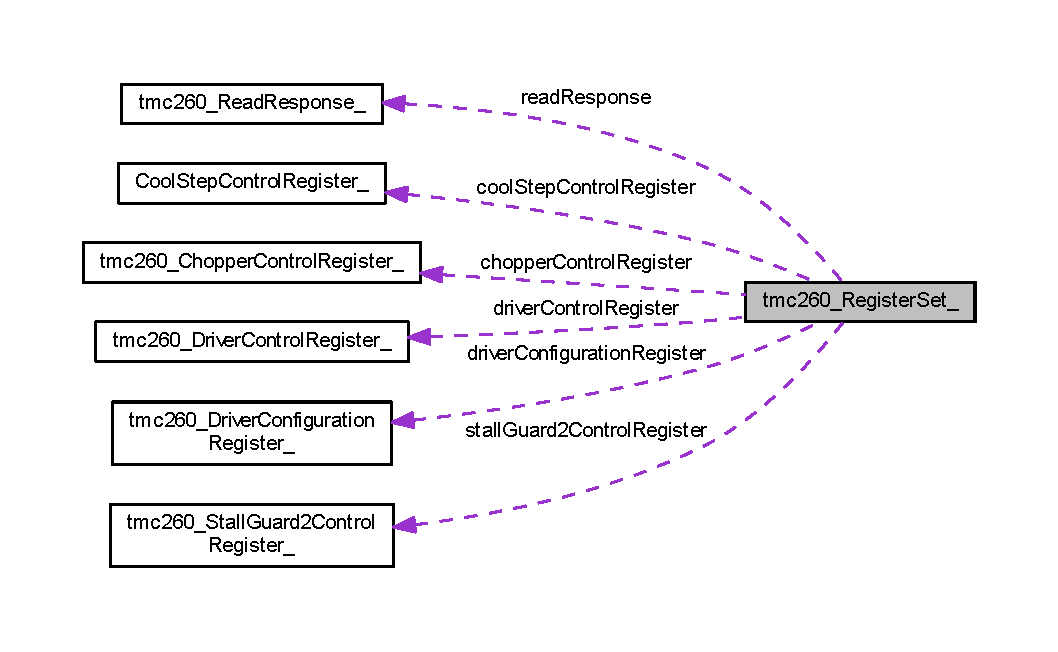
\includegraphics[width=350pt]{structtmc260___register_set____coll__graph}
\end{center}
\end{figure}
\subsection*{Data Fields}
\begin{DoxyCompactItemize}
\item 
\mbox{\hyperlink{tmc260__driver_8h_a42b84b84bc4d9625475d9ec4ed84b568}{tmc260\+\_\+\+Driver\+Control\+Register}} \mbox{\hyperlink{structtmc260___register_set___a9e19dca084d9d1634694f883273cd190}{driver\+Control\+Register}}
\item 
\mbox{\hyperlink{tmc260__driver_8h_ad9441788a191da34195daab49d56df8d}{tmc260\+\_\+\+Chopper\+Control\+Register}} \mbox{\hyperlink{structtmc260___register_set___a4f7b5272bed27e5dbdcb1e49a678a387}{chopper\+Control\+Register}}
\item 
\mbox{\hyperlink{tmc260__driver_8h_a7cfa3ad8edba4fb6683885768a43f4f4}{tmc260\+\_\+\+Cool\+Step\+Control\+Register}} \mbox{\hyperlink{structtmc260___register_set___a74101eb9a3ef24d4d5342c46ba1a2b0c}{cool\+Step\+Control\+Register}}
\item 
\mbox{\hyperlink{tmc260__driver_8h_afa0a9cd31ee349e1fea8ff665665ad45}{tmc260\+\_\+\+Stall\+Guard2\+Control\+Register}} \mbox{\hyperlink{structtmc260___register_set___a259edf50b3ce148e4cee8d78134f021b}{stall\+Guard2\+Control\+Register}}
\item 
\mbox{\hyperlink{tmc260__driver_8h_abfbbe7f0019af5812f509ef9866d375b}{tmc260\+\_\+\+Driver\+Configuration\+Register}} \mbox{\hyperlink{structtmc260___register_set___a83f35892c401a44390f622a14a1b5997}{driver\+Configuration\+Register}}
\item 
\mbox{\hyperlink{tmc260__driver_8h_a09ad0d94646027ff63c22456ac9c2436}{tmc260\+\_\+\+Read\+Response}} \mbox{\hyperlink{structtmc260___register_set___af5aca622350ed83f1c856817fb63b3c7}{read\+Response}}
\item 
int8\+\_\+t($\ast$ \mbox{\hyperlink{structtmc260___register_set___a00c49dc180ca3af071fe44406cde7d84}{send\+And\+Receive}} )(struct \mbox{\hyperlink{structtmc260___register_set__}{tmc260\+\_\+\+Register\+Set\+\_\+}} $\ast$const, \mbox{\hyperlink{tmc260__driver_8h_a4552d2ee758c08501723a6dc78d26dc7}{tmc260\+\_\+register}})
\end{DoxyCompactItemize}


\subsection{Detailed Description}
Structure to represent the registers of a tmc260 device as set of bitfields 

Definition at line 182 of file tmc260\+\_\+driver.\+h.



\subsection{Field Documentation}
\mbox{\Hypertarget{structtmc260___register_set___a4f7b5272bed27e5dbdcb1e49a678a387}\label{structtmc260___register_set___a4f7b5272bed27e5dbdcb1e49a678a387}} 
\index{tmc260\+\_\+\+Register\+Set\+\_\+@{tmc260\+\_\+\+Register\+Set\+\_\+}!chopper\+Control\+Register@{chopper\+Control\+Register}}
\index{chopper\+Control\+Register@{chopper\+Control\+Register}!tmc260\+\_\+\+Register\+Set\+\_\+@{tmc260\+\_\+\+Register\+Set\+\_\+}}
\subsubsection{\texorpdfstring{chopper\+Control\+Register}{chopperControlRegister}}
{\footnotesize\ttfamily \mbox{\hyperlink{tmc260__driver_8h_ad9441788a191da34195daab49d56df8d}{tmc260\+\_\+\+Chopper\+Control\+Register}} chopper\+Control\+Register}



Definition at line 184 of file tmc260\+\_\+driver.\+h.

\mbox{\Hypertarget{structtmc260___register_set___a74101eb9a3ef24d4d5342c46ba1a2b0c}\label{structtmc260___register_set___a74101eb9a3ef24d4d5342c46ba1a2b0c}} 
\index{tmc260\+\_\+\+Register\+Set\+\_\+@{tmc260\+\_\+\+Register\+Set\+\_\+}!cool\+Step\+Control\+Register@{cool\+Step\+Control\+Register}}
\index{cool\+Step\+Control\+Register@{cool\+Step\+Control\+Register}!tmc260\+\_\+\+Register\+Set\+\_\+@{tmc260\+\_\+\+Register\+Set\+\_\+}}
\subsubsection{\texorpdfstring{cool\+Step\+Control\+Register}{coolStepControlRegister}}
{\footnotesize\ttfamily \mbox{\hyperlink{tmc260__driver_8h_a7cfa3ad8edba4fb6683885768a43f4f4}{tmc260\+\_\+\+Cool\+Step\+Control\+Register}} cool\+Step\+Control\+Register}



Definition at line 185 of file tmc260\+\_\+driver.\+h.

\mbox{\Hypertarget{structtmc260___register_set___a83f35892c401a44390f622a14a1b5997}\label{structtmc260___register_set___a83f35892c401a44390f622a14a1b5997}} 
\index{tmc260\+\_\+\+Register\+Set\+\_\+@{tmc260\+\_\+\+Register\+Set\+\_\+}!driver\+Configuration\+Register@{driver\+Configuration\+Register}}
\index{driver\+Configuration\+Register@{driver\+Configuration\+Register}!tmc260\+\_\+\+Register\+Set\+\_\+@{tmc260\+\_\+\+Register\+Set\+\_\+}}
\subsubsection{\texorpdfstring{driver\+Configuration\+Register}{driverConfigurationRegister}}
{\footnotesize\ttfamily \mbox{\hyperlink{tmc260__driver_8h_abfbbe7f0019af5812f509ef9866d375b}{tmc260\+\_\+\+Driver\+Configuration\+Register}} driver\+Configuration\+Register}



Definition at line 187 of file tmc260\+\_\+driver.\+h.

\mbox{\Hypertarget{structtmc260___register_set___a9e19dca084d9d1634694f883273cd190}\label{structtmc260___register_set___a9e19dca084d9d1634694f883273cd190}} 
\index{tmc260\+\_\+\+Register\+Set\+\_\+@{tmc260\+\_\+\+Register\+Set\+\_\+}!driver\+Control\+Register@{driver\+Control\+Register}}
\index{driver\+Control\+Register@{driver\+Control\+Register}!tmc260\+\_\+\+Register\+Set\+\_\+@{tmc260\+\_\+\+Register\+Set\+\_\+}}
\subsubsection{\texorpdfstring{driver\+Control\+Register}{driverControlRegister}}
{\footnotesize\ttfamily \mbox{\hyperlink{tmc260__driver_8h_a42b84b84bc4d9625475d9ec4ed84b568}{tmc260\+\_\+\+Driver\+Control\+Register}} driver\+Control\+Register}



Definition at line 183 of file tmc260\+\_\+driver.\+h.

\mbox{\Hypertarget{structtmc260___register_set___af5aca622350ed83f1c856817fb63b3c7}\label{structtmc260___register_set___af5aca622350ed83f1c856817fb63b3c7}} 
\index{tmc260\+\_\+\+Register\+Set\+\_\+@{tmc260\+\_\+\+Register\+Set\+\_\+}!read\+Response@{read\+Response}}
\index{read\+Response@{read\+Response}!tmc260\+\_\+\+Register\+Set\+\_\+@{tmc260\+\_\+\+Register\+Set\+\_\+}}
\subsubsection{\texorpdfstring{read\+Response}{readResponse}}
{\footnotesize\ttfamily \mbox{\hyperlink{tmc260__driver_8h_a09ad0d94646027ff63c22456ac9c2436}{tmc260\+\_\+\+Read\+Response}} read\+Response}



Definition at line 188 of file tmc260\+\_\+driver.\+h.

\mbox{\Hypertarget{structtmc260___register_set___a00c49dc180ca3af071fe44406cde7d84}\label{structtmc260___register_set___a00c49dc180ca3af071fe44406cde7d84}} 
\index{tmc260\+\_\+\+Register\+Set\+\_\+@{tmc260\+\_\+\+Register\+Set\+\_\+}!send\+And\+Receive@{send\+And\+Receive}}
\index{send\+And\+Receive@{send\+And\+Receive}!tmc260\+\_\+\+Register\+Set\+\_\+@{tmc260\+\_\+\+Register\+Set\+\_\+}}
\subsubsection{\texorpdfstring{send\+And\+Receive}{sendAndReceive}}
{\footnotesize\ttfamily int8\+\_\+t($\ast$  send\+And\+Receive) (struct \mbox{\hyperlink{structtmc260___register_set__}{tmc260\+\_\+\+Register\+Set\+\_\+}} $\ast$const, \mbox{\hyperlink{tmc260__driver_8h_a4552d2ee758c08501723a6dc78d26dc7}{tmc260\+\_\+register}})}



Definition at line 189 of file tmc260\+\_\+driver.\+h.

\mbox{\Hypertarget{structtmc260___register_set___a259edf50b3ce148e4cee8d78134f021b}\label{structtmc260___register_set___a259edf50b3ce148e4cee8d78134f021b}} 
\index{tmc260\+\_\+\+Register\+Set\+\_\+@{tmc260\+\_\+\+Register\+Set\+\_\+}!stall\+Guard2\+Control\+Register@{stall\+Guard2\+Control\+Register}}
\index{stall\+Guard2\+Control\+Register@{stall\+Guard2\+Control\+Register}!tmc260\+\_\+\+Register\+Set\+\_\+@{tmc260\+\_\+\+Register\+Set\+\_\+}}
\subsubsection{\texorpdfstring{stall\+Guard2\+Control\+Register}{stallGuard2ControlRegister}}
{\footnotesize\ttfamily \mbox{\hyperlink{tmc260__driver_8h_afa0a9cd31ee349e1fea8ff665665ad45}{tmc260\+\_\+\+Stall\+Guard2\+Control\+Register}} stall\+Guard2\+Control\+Register}



Definition at line 186 of file tmc260\+\_\+driver.\+h.



The documentation for this struct was generated from the following file\+:\begin{DoxyCompactItemize}
\item 
Library/\+Library/inc/\mbox{\hyperlink{tmc260__driver_8h}{tmc260\+\_\+driver.\+h}}\end{DoxyCompactItemize}

\hypertarget{uniontmc260___stall_guard2_control_register__}{}\section{tmc260\+\_\+\+Stall\+Guard2\+Control\+Register\+\_\+ Union Reference}
\label{uniontmc260___stall_guard2_control_register__}\index{tmc260\+\_\+\+Stall\+Guard2\+Control\+Register\+\_\+@{tmc260\+\_\+\+Stall\+Guard2\+Control\+Register\+\_\+}}


{\ttfamily \#include $<$tmc260\+\_\+driver.\+h$>$}

\subsection*{Data Fields}
\begin{DoxyCompactItemize}
\item 
\mbox{\hyperlink{tmc260__driver_8h_a280b01a3b5bb4294fcee278b00c030d6}{Register}} \mbox{\hyperlink{uniontmc260___stall_guard2_control_register___a445b72174063a88455cd86c22d77d03f}{bytes}}
\item 
\begin{tabbing}
xx\=xx\=xx\=xx\=xx\=xx\=xx\=xx\=xx\=\kill
struct \{\\
\>uint32\_t \mbox{\hyperlink{uniontmc260___stall_guard2_control_register___af3aaac138d1ebeba8461dc779f2fde1e}{currentScale}}: 5\\
\>uint32\_t \mbox{\hyperlink{uniontmc260___stall_guard2_control_register___aa5d9ea4624bf97017a821a70177c6bdb}{reserved\_1}}: 1\\
\>uint32\_t \mbox{\hyperlink{uniontmc260___stall_guard2_control_register___a50b223df92282d04dfa46306b53a9905}{reserved\_2}}: 1\\
\>uint32\_t \mbox{\hyperlink{uniontmc260___stall_guard2_control_register___af8407645db2d0329264f3c6d0cbd6dd1}{reserved\_3}}: 1\\
\>uint32\_t \mbox{\hyperlink{uniontmc260___stall_guard2_control_register___a9bdf286986dabc8efc07fc3a91f2c006}{stallGuard2ThresholdValue}}: 7\\
\>uint32\_t \mbox{\hyperlink{uniontmc260___stall_guard2_control_register___aaf2eb7a7615ec891d7e5a9d49d433f37}{reserved\_4}}: 1\\
\>uint32\_t \mbox{\hyperlink{uniontmc260___stall_guard2_control_register___ac982627270dc352b27db00b232df6108}{stallGuard2FilterEnable}}: 1\\
\>uint32\_t \mbox{\hyperlink{uniontmc260___stall_guard2_control_register___a8e58d0701295971bc3d890f5107f8aa5}{registerAdressBit\_1}}: 1\\
\>uint32\_t \mbox{\hyperlink{uniontmc260___stall_guard2_control_register___abd6d1c957737511340b85f5c2d61f9ab}{registerAdressBit\_2}}: 1\\
\>uint32\_t \mbox{\hyperlink{uniontmc260___stall_guard2_control_register___a3da0387ab629039b91d051ab328910f0}{registerAdressBit\_3}}: 1\\
\>uint32\_t \mbox{\hyperlink{uniontmc260___stall_guard2_control_register___a3e57c2ef1c3ffb36722f000cc1156824}{\_\_pad0\_\_}}: 4\\
\} \mbox{\hyperlink{uniontmc260___stall_guard2_control_register___abdba31969268596a81e094d5f9f59c05}{bits}}\\

\end{tabbing}\end{DoxyCompactItemize}


\subsection{Detailed Description}
Union to represent the stall\+Guard2 control register (S\+G\+C\+S\+C\+O\+NF) of a tmc260 device as bitfield 

Definition at line 99 of file tmc260\+\_\+driver.\+h.



\subsection{Field Documentation}
\mbox{\Hypertarget{uniontmc260___stall_guard2_control_register___a3e57c2ef1c3ffb36722f000cc1156824}\label{uniontmc260___stall_guard2_control_register___a3e57c2ef1c3ffb36722f000cc1156824}} 
\index{tmc260\+\_\+\+Stall\+Guard2\+Control\+Register\+\_\+@{tmc260\+\_\+\+Stall\+Guard2\+Control\+Register\+\_\+}!\+\_\+\+\_\+pad0\+\_\+\+\_\+@{\+\_\+\+\_\+pad0\+\_\+\+\_\+}}
\index{\+\_\+\+\_\+pad0\+\_\+\+\_\+@{\+\_\+\+\_\+pad0\+\_\+\+\_\+}!tmc260\+\_\+\+Stall\+Guard2\+Control\+Register\+\_\+@{tmc260\+\_\+\+Stall\+Guard2\+Control\+Register\+\_\+}}
\subsubsection{\texorpdfstring{\+\_\+\+\_\+pad0\+\_\+\+\_\+}{\_\_pad0\_\_}}
{\footnotesize\ttfamily uint32\+\_\+t \+\_\+\+\_\+pad0\+\_\+\+\_\+}



Definition at line 112 of file tmc260\+\_\+driver.\+h.

\mbox{\Hypertarget{uniontmc260___stall_guard2_control_register___abdba31969268596a81e094d5f9f59c05}\label{uniontmc260___stall_guard2_control_register___abdba31969268596a81e094d5f9f59c05}} 
\index{tmc260\+\_\+\+Stall\+Guard2\+Control\+Register\+\_\+@{tmc260\+\_\+\+Stall\+Guard2\+Control\+Register\+\_\+}!bits@{bits}}
\index{bits@{bits}!tmc260\+\_\+\+Stall\+Guard2\+Control\+Register\+\_\+@{tmc260\+\_\+\+Stall\+Guard2\+Control\+Register\+\_\+}}
\subsubsection{\texorpdfstring{bits}{bits}}
{\footnotesize\ttfamily struct \{ ... \}  bits}

\mbox{\Hypertarget{uniontmc260___stall_guard2_control_register___a445b72174063a88455cd86c22d77d03f}\label{uniontmc260___stall_guard2_control_register___a445b72174063a88455cd86c22d77d03f}} 
\index{tmc260\+\_\+\+Stall\+Guard2\+Control\+Register\+\_\+@{tmc260\+\_\+\+Stall\+Guard2\+Control\+Register\+\_\+}!bytes@{bytes}}
\index{bytes@{bytes}!tmc260\+\_\+\+Stall\+Guard2\+Control\+Register\+\_\+@{tmc260\+\_\+\+Stall\+Guard2\+Control\+Register\+\_\+}}
\subsubsection{\texorpdfstring{bytes}{bytes}}
{\footnotesize\ttfamily \mbox{\hyperlink{tmc260__driver_8h_a280b01a3b5bb4294fcee278b00c030d6}{Register}} bytes}



Definition at line 100 of file tmc260\+\_\+driver.\+h.

\mbox{\Hypertarget{uniontmc260___stall_guard2_control_register___af3aaac138d1ebeba8461dc779f2fde1e}\label{uniontmc260___stall_guard2_control_register___af3aaac138d1ebeba8461dc779f2fde1e}} 
\index{tmc260\+\_\+\+Stall\+Guard2\+Control\+Register\+\_\+@{tmc260\+\_\+\+Stall\+Guard2\+Control\+Register\+\_\+}!current\+Scale@{current\+Scale}}
\index{current\+Scale@{current\+Scale}!tmc260\+\_\+\+Stall\+Guard2\+Control\+Register\+\_\+@{tmc260\+\_\+\+Stall\+Guard2\+Control\+Register\+\_\+}}
\subsubsection{\texorpdfstring{current\+Scale}{currentScale}}
{\footnotesize\ttfamily uint32\+\_\+t current\+Scale}



Definition at line 102 of file tmc260\+\_\+driver.\+h.

\mbox{\Hypertarget{uniontmc260___stall_guard2_control_register___a8e58d0701295971bc3d890f5107f8aa5}\label{uniontmc260___stall_guard2_control_register___a8e58d0701295971bc3d890f5107f8aa5}} 
\index{tmc260\+\_\+\+Stall\+Guard2\+Control\+Register\+\_\+@{tmc260\+\_\+\+Stall\+Guard2\+Control\+Register\+\_\+}!register\+Adress\+Bit\+\_\+1@{register\+Adress\+Bit\+\_\+1}}
\index{register\+Adress\+Bit\+\_\+1@{register\+Adress\+Bit\+\_\+1}!tmc260\+\_\+\+Stall\+Guard2\+Control\+Register\+\_\+@{tmc260\+\_\+\+Stall\+Guard2\+Control\+Register\+\_\+}}
\subsubsection{\texorpdfstring{register\+Adress\+Bit\+\_\+1}{registerAdressBit\_1}}
{\footnotesize\ttfamily uint32\+\_\+t register\+Adress\+Bit\+\_\+1}



Definition at line 109 of file tmc260\+\_\+driver.\+h.

\mbox{\Hypertarget{uniontmc260___stall_guard2_control_register___abd6d1c957737511340b85f5c2d61f9ab}\label{uniontmc260___stall_guard2_control_register___abd6d1c957737511340b85f5c2d61f9ab}} 
\index{tmc260\+\_\+\+Stall\+Guard2\+Control\+Register\+\_\+@{tmc260\+\_\+\+Stall\+Guard2\+Control\+Register\+\_\+}!register\+Adress\+Bit\+\_\+2@{register\+Adress\+Bit\+\_\+2}}
\index{register\+Adress\+Bit\+\_\+2@{register\+Adress\+Bit\+\_\+2}!tmc260\+\_\+\+Stall\+Guard2\+Control\+Register\+\_\+@{tmc260\+\_\+\+Stall\+Guard2\+Control\+Register\+\_\+}}
\subsubsection{\texorpdfstring{register\+Adress\+Bit\+\_\+2}{registerAdressBit\_2}}
{\footnotesize\ttfamily uint32\+\_\+t register\+Adress\+Bit\+\_\+2}



Definition at line 110 of file tmc260\+\_\+driver.\+h.

\mbox{\Hypertarget{uniontmc260___stall_guard2_control_register___a3da0387ab629039b91d051ab328910f0}\label{uniontmc260___stall_guard2_control_register___a3da0387ab629039b91d051ab328910f0}} 
\index{tmc260\+\_\+\+Stall\+Guard2\+Control\+Register\+\_\+@{tmc260\+\_\+\+Stall\+Guard2\+Control\+Register\+\_\+}!register\+Adress\+Bit\+\_\+3@{register\+Adress\+Bit\+\_\+3}}
\index{register\+Adress\+Bit\+\_\+3@{register\+Adress\+Bit\+\_\+3}!tmc260\+\_\+\+Stall\+Guard2\+Control\+Register\+\_\+@{tmc260\+\_\+\+Stall\+Guard2\+Control\+Register\+\_\+}}
\subsubsection{\texorpdfstring{register\+Adress\+Bit\+\_\+3}{registerAdressBit\_3}}
{\footnotesize\ttfamily uint32\+\_\+t register\+Adress\+Bit\+\_\+3}



Definition at line 111 of file tmc260\+\_\+driver.\+h.

\mbox{\Hypertarget{uniontmc260___stall_guard2_control_register___aa5d9ea4624bf97017a821a70177c6bdb}\label{uniontmc260___stall_guard2_control_register___aa5d9ea4624bf97017a821a70177c6bdb}} 
\index{tmc260\+\_\+\+Stall\+Guard2\+Control\+Register\+\_\+@{tmc260\+\_\+\+Stall\+Guard2\+Control\+Register\+\_\+}!reserved\+\_\+1@{reserved\+\_\+1}}
\index{reserved\+\_\+1@{reserved\+\_\+1}!tmc260\+\_\+\+Stall\+Guard2\+Control\+Register\+\_\+@{tmc260\+\_\+\+Stall\+Guard2\+Control\+Register\+\_\+}}
\subsubsection{\texorpdfstring{reserved\+\_\+1}{reserved\_1}}
{\footnotesize\ttfamily uint32\+\_\+t reserved\+\_\+1}



Definition at line 103 of file tmc260\+\_\+driver.\+h.

\mbox{\Hypertarget{uniontmc260___stall_guard2_control_register___a50b223df92282d04dfa46306b53a9905}\label{uniontmc260___stall_guard2_control_register___a50b223df92282d04dfa46306b53a9905}} 
\index{tmc260\+\_\+\+Stall\+Guard2\+Control\+Register\+\_\+@{tmc260\+\_\+\+Stall\+Guard2\+Control\+Register\+\_\+}!reserved\+\_\+2@{reserved\+\_\+2}}
\index{reserved\+\_\+2@{reserved\+\_\+2}!tmc260\+\_\+\+Stall\+Guard2\+Control\+Register\+\_\+@{tmc260\+\_\+\+Stall\+Guard2\+Control\+Register\+\_\+}}
\subsubsection{\texorpdfstring{reserved\+\_\+2}{reserved\_2}}
{\footnotesize\ttfamily uint32\+\_\+t reserved\+\_\+2}



Definition at line 104 of file tmc260\+\_\+driver.\+h.

\mbox{\Hypertarget{uniontmc260___stall_guard2_control_register___af8407645db2d0329264f3c6d0cbd6dd1}\label{uniontmc260___stall_guard2_control_register___af8407645db2d0329264f3c6d0cbd6dd1}} 
\index{tmc260\+\_\+\+Stall\+Guard2\+Control\+Register\+\_\+@{tmc260\+\_\+\+Stall\+Guard2\+Control\+Register\+\_\+}!reserved\+\_\+3@{reserved\+\_\+3}}
\index{reserved\+\_\+3@{reserved\+\_\+3}!tmc260\+\_\+\+Stall\+Guard2\+Control\+Register\+\_\+@{tmc260\+\_\+\+Stall\+Guard2\+Control\+Register\+\_\+}}
\subsubsection{\texorpdfstring{reserved\+\_\+3}{reserved\_3}}
{\footnotesize\ttfamily uint32\+\_\+t reserved\+\_\+3}



Definition at line 105 of file tmc260\+\_\+driver.\+h.

\mbox{\Hypertarget{uniontmc260___stall_guard2_control_register___aaf2eb7a7615ec891d7e5a9d49d433f37}\label{uniontmc260___stall_guard2_control_register___aaf2eb7a7615ec891d7e5a9d49d433f37}} 
\index{tmc260\+\_\+\+Stall\+Guard2\+Control\+Register\+\_\+@{tmc260\+\_\+\+Stall\+Guard2\+Control\+Register\+\_\+}!reserved\+\_\+4@{reserved\+\_\+4}}
\index{reserved\+\_\+4@{reserved\+\_\+4}!tmc260\+\_\+\+Stall\+Guard2\+Control\+Register\+\_\+@{tmc260\+\_\+\+Stall\+Guard2\+Control\+Register\+\_\+}}
\subsubsection{\texorpdfstring{reserved\+\_\+4}{reserved\_4}}
{\footnotesize\ttfamily uint32\+\_\+t reserved\+\_\+4}



Definition at line 107 of file tmc260\+\_\+driver.\+h.

\mbox{\Hypertarget{uniontmc260___stall_guard2_control_register___ac982627270dc352b27db00b232df6108}\label{uniontmc260___stall_guard2_control_register___ac982627270dc352b27db00b232df6108}} 
\index{tmc260\+\_\+\+Stall\+Guard2\+Control\+Register\+\_\+@{tmc260\+\_\+\+Stall\+Guard2\+Control\+Register\+\_\+}!stall\+Guard2\+Filter\+Enable@{stall\+Guard2\+Filter\+Enable}}
\index{stall\+Guard2\+Filter\+Enable@{stall\+Guard2\+Filter\+Enable}!tmc260\+\_\+\+Stall\+Guard2\+Control\+Register\+\_\+@{tmc260\+\_\+\+Stall\+Guard2\+Control\+Register\+\_\+}}
\subsubsection{\texorpdfstring{stall\+Guard2\+Filter\+Enable}{stallGuard2FilterEnable}}
{\footnotesize\ttfamily uint32\+\_\+t stall\+Guard2\+Filter\+Enable}



Definition at line 108 of file tmc260\+\_\+driver.\+h.

\mbox{\Hypertarget{uniontmc260___stall_guard2_control_register___a9bdf286986dabc8efc07fc3a91f2c006}\label{uniontmc260___stall_guard2_control_register___a9bdf286986dabc8efc07fc3a91f2c006}} 
\index{tmc260\+\_\+\+Stall\+Guard2\+Control\+Register\+\_\+@{tmc260\+\_\+\+Stall\+Guard2\+Control\+Register\+\_\+}!stall\+Guard2\+Threshold\+Value@{stall\+Guard2\+Threshold\+Value}}
\index{stall\+Guard2\+Threshold\+Value@{stall\+Guard2\+Threshold\+Value}!tmc260\+\_\+\+Stall\+Guard2\+Control\+Register\+\_\+@{tmc260\+\_\+\+Stall\+Guard2\+Control\+Register\+\_\+}}
\subsubsection{\texorpdfstring{stall\+Guard2\+Threshold\+Value}{stallGuard2ThresholdValue}}
{\footnotesize\ttfamily uint32\+\_\+t stall\+Guard2\+Threshold\+Value}



Definition at line 106 of file tmc260\+\_\+driver.\+h.



The documentation for this union was generated from the following file\+:\begin{DoxyCompactItemize}
\item 
Library/\+Library/inc/\mbox{\hyperlink{tmc260__driver_8h}{tmc260\+\_\+driver.\+h}}\end{DoxyCompactItemize}

\chapter{File Documentation}
\hypertarget{adc_8h}{}\section{adc.\+h File Reference}
\label{adc_8h}\index{adc.\+h@{adc.\+h}}
{\ttfamily \#include \char`\"{}stm32f4xx\+\_\+hal.\+h\char`\"{}}\newline
{\ttfamily \#include \char`\"{}main.\+h\char`\"{}}\newline
Include dependency graph for adc.\+h\+:\nopagebreak
\begin{figure}[H]
\begin{center}
\leavevmode
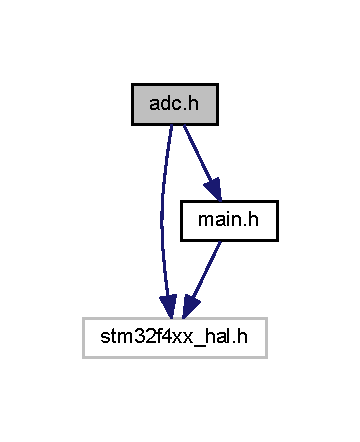
\includegraphics[width=173pt]{adc_8h__incl}
\end{center}
\end{figure}
This graph shows which files directly or indirectly include this file\+:\nopagebreak
\begin{figure}[H]
\begin{center}
\leavevmode
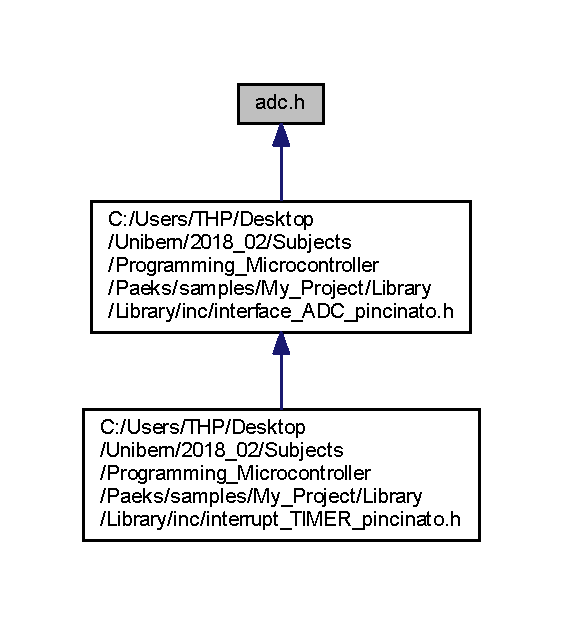
\includegraphics[width=270pt]{adc_8h__dep__incl}
\end{center}
\end{figure}
\subsection*{Functions}
\begin{DoxyCompactItemize}
\item 
void \mbox{\hyperlink{adc_8h_a47642651029b93e3f9c9edad46bd27b4}{\+\_\+\+Error\+\_\+\+Handler}} (char $\ast$, int)
\item 
void \mbox{\hyperlink{adc_8h_acccd58aa70215a6b184ad242312ffd0c}{M\+X\+\_\+\+A\+D\+C1\+\_\+\+Init}} (void)
\item 
void \mbox{\hyperlink{adc_8h_a101e2e3433dfe72bbbd0ae3a84489263}{M\+X\+\_\+\+A\+D\+C2\+\_\+\+Init}} (void)
\end{DoxyCompactItemize}
\subsection*{Variables}
\begin{DoxyCompactItemize}
\item 
A\+D\+C\+\_\+\+Handle\+Type\+Def \mbox{\hyperlink{adc_8h_a22b804736f5648d52f639b2647d4ed13}{hadc1}}
\item 
A\+D\+C\+\_\+\+Handle\+Type\+Def \mbox{\hyperlink{adc_8h_acd9221f1aa19aebfe0b744947f2daf49}{hadc2}}
\end{DoxyCompactItemize}


\subsection{Function Documentation}
\mbox{\Hypertarget{adc_8h_a47642651029b93e3f9c9edad46bd27b4}\label{adc_8h_a47642651029b93e3f9c9edad46bd27b4}} 
\index{adc.\+h@{adc.\+h}!\+\_\+\+Error\+\_\+\+Handler@{\+\_\+\+Error\+\_\+\+Handler}}
\index{\+\_\+\+Error\+\_\+\+Handler@{\+\_\+\+Error\+\_\+\+Handler}!adc.\+h@{adc.\+h}}
\subsubsection{\texorpdfstring{\+\_\+\+Error\+\_\+\+Handler()}{\_Error\_Handler()}}
{\footnotesize\ttfamily void \+\_\+\+Error\+\_\+\+Handler (\begin{DoxyParamCaption}\item[{char $\ast$}]{,  }\item[{int}]{ }\end{DoxyParamCaption})}

\mbox{\Hypertarget{adc_8h_acccd58aa70215a6b184ad242312ffd0c}\label{adc_8h_acccd58aa70215a6b184ad242312ffd0c}} 
\index{adc.\+h@{adc.\+h}!M\+X\+\_\+\+A\+D\+C1\+\_\+\+Init@{M\+X\+\_\+\+A\+D\+C1\+\_\+\+Init}}
\index{M\+X\+\_\+\+A\+D\+C1\+\_\+\+Init@{M\+X\+\_\+\+A\+D\+C1\+\_\+\+Init}!adc.\+h@{adc.\+h}}
\subsubsection{\texorpdfstring{M\+X\+\_\+\+A\+D\+C1\+\_\+\+Init()}{MX\_ADC1\_Init()}}
{\footnotesize\ttfamily void M\+X\+\_\+\+A\+D\+C1\+\_\+\+Init (\begin{DoxyParamCaption}\item[{void}]{ }\end{DoxyParamCaption})}

\mbox{\Hypertarget{adc_8h_a101e2e3433dfe72bbbd0ae3a84489263}\label{adc_8h_a101e2e3433dfe72bbbd0ae3a84489263}} 
\index{adc.\+h@{adc.\+h}!M\+X\+\_\+\+A\+D\+C2\+\_\+\+Init@{M\+X\+\_\+\+A\+D\+C2\+\_\+\+Init}}
\index{M\+X\+\_\+\+A\+D\+C2\+\_\+\+Init@{M\+X\+\_\+\+A\+D\+C2\+\_\+\+Init}!adc.\+h@{adc.\+h}}
\subsubsection{\texorpdfstring{M\+X\+\_\+\+A\+D\+C2\+\_\+\+Init()}{MX\_ADC2\_Init()}}
{\footnotesize\ttfamily void M\+X\+\_\+\+A\+D\+C2\+\_\+\+Init (\begin{DoxyParamCaption}\item[{void}]{ }\end{DoxyParamCaption})}



\subsection{Variable Documentation}
\mbox{\Hypertarget{adc_8h_a22b804736f5648d52f639b2647d4ed13}\label{adc_8h_a22b804736f5648d52f639b2647d4ed13}} 
\index{adc.\+h@{adc.\+h}!hadc1@{hadc1}}
\index{hadc1@{hadc1}!adc.\+h@{adc.\+h}}
\subsubsection{\texorpdfstring{hadc1}{hadc1}}
{\footnotesize\ttfamily A\+D\+C\+\_\+\+Handle\+Type\+Def hadc1}

File Name \+: \mbox{\hyperlink{adc_8h}{A\+D\+C.\+h}} Description \+: This file provides code for the configuration of the A\+DC instances.

This notice applies to any and all portions of this file that are not between comment pairs U\+S\+ER C\+O\+DE B\+E\+G\+IN and U\+S\+ER C\+O\+DE E\+ND. Other portions of this file, whether inserted by the user or by software development tools are owned by their respective copyright owners.

Copyright (c) 2018 S\+T\+Microelectronics International N.\+V. All rights reserved.

Redistribution and use in source and binary forms, with or without modification, are permitted, provided that the following conditions are met\+:


\begin{DoxyEnumerate}
\item Redistribution of source code must retain the above copyright notice, this list of conditions and the following disclaimer.
\item Redistributions in binary form must reproduce the above copyright notice, this list of conditions and the following disclaimer in the documentation and/or other materials provided with the distribution.
\item Neither the name of S\+T\+Microelectronics nor the names of other contributors to this software may be used to endorse or promote products derived from this software without specific written permission.
\item This software, including modifications and/or derivative works of this software, must execute solely and exclusively on microcontroller or microprocessor devices manufactured by or for S\+T\+Microelectronics.
\item Redistribution and use of this software other than as permitted under this license is void and will automatically terminate your rights under this license.
\end{DoxyEnumerate}

T\+H\+IS S\+O\+F\+T\+W\+A\+RE IS P\+R\+O\+V\+I\+D\+ED BY S\+T\+M\+I\+C\+R\+O\+E\+L\+E\+C\+T\+R\+O\+N\+I\+CS A\+ND C\+O\+N\+T\+R\+I\+B\+U\+T\+O\+RS \char`\"{}\+A\+S I\+S\char`\"{} A\+ND A\+NY E\+X\+P\+R\+E\+SS, I\+M\+P\+L\+I\+ED OR S\+T\+A\+T\+U\+T\+O\+RY W\+A\+R\+R\+A\+N\+T\+I\+ES, I\+N\+C\+L\+U\+D\+I\+NG, B\+UT N\+OT L\+I\+M\+I\+T\+ED TO, T\+HE I\+M\+P\+L\+I\+ED W\+A\+R\+R\+A\+N\+T\+I\+ES OF M\+E\+R\+C\+H\+A\+N\+T\+A\+B\+I\+L\+I\+TY, F\+I\+T\+N\+E\+SS F\+OR A P\+A\+R\+T\+I\+C\+U\+L\+AR P\+U\+R\+P\+O\+SE A\+ND N\+O\+N-\/\+I\+N\+F\+R\+I\+N\+G\+E\+M\+E\+NT OF T\+H\+I\+RD P\+A\+R\+TY I\+N\+T\+E\+L\+L\+E\+C\+T\+U\+AL P\+R\+O\+P\+E\+R\+TY R\+I\+G\+H\+TS A\+RE D\+I\+S\+C\+L\+A\+I\+M\+ED TO T\+HE F\+U\+L\+L\+E\+ST E\+X\+T\+E\+NT P\+E\+R\+M\+I\+T\+T\+ED BY L\+AW. IN NO E\+V\+E\+NT S\+H\+A\+LL S\+T\+M\+I\+C\+R\+O\+E\+L\+E\+C\+T\+R\+O\+N\+I\+CS OR C\+O\+N\+T\+R\+I\+B\+U\+T\+O\+RS BE L\+I\+A\+B\+LE F\+OR A\+NY D\+I\+R\+E\+CT, I\+N\+D\+I\+R\+E\+CT, I\+N\+C\+I\+D\+E\+N\+T\+AL, S\+P\+E\+C\+I\+AL, E\+X\+E\+M\+P\+L\+A\+RY, OR C\+O\+N\+S\+E\+Q\+U\+E\+N\+T\+I\+AL D\+A\+M\+A\+G\+ES (I\+N\+C\+L\+U\+D\+I\+NG, B\+UT N\+OT L\+I\+M\+I\+T\+ED TO, P\+R\+O\+C\+U\+R\+E\+M\+E\+NT OF S\+U\+B\+S\+T\+I\+T\+U\+TE G\+O\+O\+DS OR S\+E\+R\+V\+I\+C\+ES; L\+O\+SS OF U\+SE, D\+A\+TA, OR P\+R\+O\+F\+I\+TS; OR B\+U\+S\+I\+N\+E\+SS I\+N\+T\+E\+R\+R\+U\+P\+T\+I\+ON) H\+O\+W\+E\+V\+ER C\+A\+U\+S\+ED A\+ND ON A\+NY T\+H\+E\+O\+RY OF L\+I\+A\+B\+I\+L\+I\+TY, W\+H\+E\+T\+H\+ER IN C\+O\+N\+T\+R\+A\+CT, S\+T\+R\+I\+CT L\+I\+A\+B\+I\+L\+I\+TY, OR T\+O\+RT (I\+N\+C\+L\+U\+D\+I\+NG N\+E\+G\+L\+I\+G\+E\+N\+CE OR O\+T\+H\+E\+R\+W\+I\+SE) A\+R\+I\+S\+I\+NG IN A\+NY W\+AY O\+UT OF T\+HE U\+SE OF T\+H\+IS S\+O\+F\+T\+W\+A\+RE, E\+V\+EN IF A\+D\+V\+I\+S\+ED OF T\+HE P\+O\+S\+S\+I\+B\+I\+L\+I\+TY OF S\+U\+CH D\+A\+M\+A\+GE. \mbox{\Hypertarget{adc_8h_acd9221f1aa19aebfe0b744947f2daf49}\label{adc_8h_acd9221f1aa19aebfe0b744947f2daf49}} 
\index{adc.\+h@{adc.\+h}!hadc2@{hadc2}}
\index{hadc2@{hadc2}!adc.\+h@{adc.\+h}}
\subsubsection{\texorpdfstring{hadc2}{hadc2}}
{\footnotesize\ttfamily A\+D\+C\+\_\+\+Handle\+Type\+Def hadc2}


\hypertarget{dma_8h}{}\section{dma.\+h File Reference}
\label{dma_8h}\index{dma.\+h@{dma.\+h}}
{\ttfamily \#include \char`\"{}stm32f4xx\+\_\+hal.\+h\char`\"{}}\newline
{\ttfamily \#include \char`\"{}main.\+h\char`\"{}}\newline
Include dependency graph for dma.\+h\+:\nopagebreak
\begin{figure}[H]
\begin{center}
\leavevmode
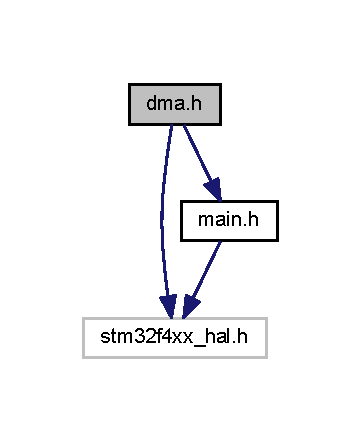
\includegraphics[width=173pt]{dma_8h__incl}
\end{center}
\end{figure}
This graph shows which files directly or indirectly include this file\+:\nopagebreak
\begin{figure}[H]
\begin{center}
\leavevmode
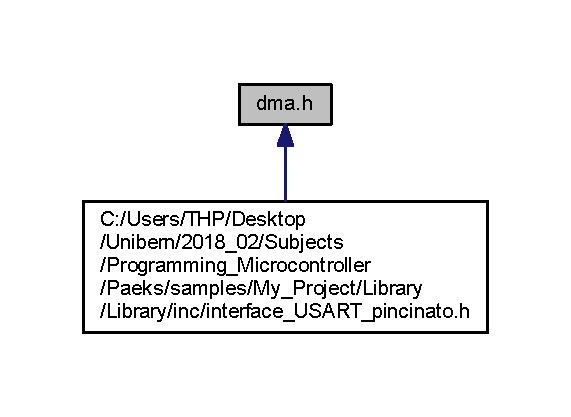
\includegraphics[width=274pt]{dma_8h__dep__incl}
\end{center}
\end{figure}
\subsection*{Functions}
\begin{DoxyCompactItemize}
\item 
void \mbox{\hyperlink{dma_8h_a47642651029b93e3f9c9edad46bd27b4}{\+\_\+\+Error\+\_\+\+Handler}} (char $\ast$, int)
\item 
void \mbox{\hyperlink{dma_8h_a323249dac769f9855c10b4ec9446b707}{M\+X\+\_\+\+D\+M\+A\+\_\+\+Init}} (void)
\end{DoxyCompactItemize}


\subsection{Function Documentation}
\mbox{\Hypertarget{dma_8h_a47642651029b93e3f9c9edad46bd27b4}\label{dma_8h_a47642651029b93e3f9c9edad46bd27b4}} 
\index{dma.\+h@{dma.\+h}!\+\_\+\+Error\+\_\+\+Handler@{\+\_\+\+Error\+\_\+\+Handler}}
\index{\+\_\+\+Error\+\_\+\+Handler@{\+\_\+\+Error\+\_\+\+Handler}!dma.\+h@{dma.\+h}}
\subsubsection{\texorpdfstring{\+\_\+\+Error\+\_\+\+Handler()}{\_Error\_Handler()}}
{\footnotesize\ttfamily void \+\_\+\+Error\+\_\+\+Handler (\begin{DoxyParamCaption}\item[{char $\ast$}]{,  }\item[{int}]{ }\end{DoxyParamCaption})}

File Name \+: \mbox{\hyperlink{dma_8h}{dma.\+h}} Description \+: This file contains all the function prototypes for the dma.\+c file

This notice applies to any and all portions of this file that are not between comment pairs U\+S\+ER C\+O\+DE B\+E\+G\+IN and U\+S\+ER C\+O\+DE E\+ND. Other portions of this file, whether inserted by the user or by software development tools are owned by their respective copyright owners.

Copyright (c) 2018 S\+T\+Microelectronics International N.\+V. All rights reserved.

Redistribution and use in source and binary forms, with or without modification, are permitted, provided that the following conditions are met\+:


\begin{DoxyEnumerate}
\item Redistribution of source code must retain the above copyright notice, this list of conditions and the following disclaimer.
\item Redistributions in binary form must reproduce the above copyright notice, this list of conditions and the following disclaimer in the documentation and/or other materials provided with the distribution.
\item Neither the name of S\+T\+Microelectronics nor the names of other contributors to this software may be used to endorse or promote products derived from this software without specific written permission.
\item This software, including modifications and/or derivative works of this software, must execute solely and exclusively on microcontroller or microprocessor devices manufactured by or for S\+T\+Microelectronics.
\item Redistribution and use of this software other than as permitted under this license is void and will automatically terminate your rights under this license.
\end{DoxyEnumerate}

T\+H\+IS S\+O\+F\+T\+W\+A\+RE IS P\+R\+O\+V\+I\+D\+ED BY S\+T\+M\+I\+C\+R\+O\+E\+L\+E\+C\+T\+R\+O\+N\+I\+CS A\+ND C\+O\+N\+T\+R\+I\+B\+U\+T\+O\+RS \char`\"{}\+A\+S I\+S\char`\"{} A\+ND A\+NY E\+X\+P\+R\+E\+SS, I\+M\+P\+L\+I\+ED OR S\+T\+A\+T\+U\+T\+O\+RY W\+A\+R\+R\+A\+N\+T\+I\+ES, I\+N\+C\+L\+U\+D\+I\+NG, B\+UT N\+OT L\+I\+M\+I\+T\+ED TO, T\+HE I\+M\+P\+L\+I\+ED W\+A\+R\+R\+A\+N\+T\+I\+ES OF M\+E\+R\+C\+H\+A\+N\+T\+A\+B\+I\+L\+I\+TY, F\+I\+T\+N\+E\+SS F\+OR A P\+A\+R\+T\+I\+C\+U\+L\+AR P\+U\+R\+P\+O\+SE A\+ND N\+O\+N-\/\+I\+N\+F\+R\+I\+N\+G\+E\+M\+E\+NT OF T\+H\+I\+RD P\+A\+R\+TY I\+N\+T\+E\+L\+L\+E\+C\+T\+U\+AL P\+R\+O\+P\+E\+R\+TY R\+I\+G\+H\+TS A\+RE D\+I\+S\+C\+L\+A\+I\+M\+ED TO T\+HE F\+U\+L\+L\+E\+ST E\+X\+T\+E\+NT P\+E\+R\+M\+I\+T\+T\+ED BY L\+AW. IN NO E\+V\+E\+NT S\+H\+A\+LL S\+T\+M\+I\+C\+R\+O\+E\+L\+E\+C\+T\+R\+O\+N\+I\+CS OR C\+O\+N\+T\+R\+I\+B\+U\+T\+O\+RS BE L\+I\+A\+B\+LE F\+OR A\+NY D\+I\+R\+E\+CT, I\+N\+D\+I\+R\+E\+CT, I\+N\+C\+I\+D\+E\+N\+T\+AL, S\+P\+E\+C\+I\+AL, E\+X\+E\+M\+P\+L\+A\+RY, OR C\+O\+N\+S\+E\+Q\+U\+E\+N\+T\+I\+AL D\+A\+M\+A\+G\+ES (I\+N\+C\+L\+U\+D\+I\+NG, B\+UT N\+OT L\+I\+M\+I\+T\+ED TO, P\+R\+O\+C\+U\+R\+E\+M\+E\+NT OF S\+U\+B\+S\+T\+I\+T\+U\+TE G\+O\+O\+DS OR S\+E\+R\+V\+I\+C\+ES; L\+O\+SS OF U\+SE, D\+A\+TA, OR P\+R\+O\+F\+I\+TS; OR B\+U\+S\+I\+N\+E\+SS I\+N\+T\+E\+R\+R\+U\+P\+T\+I\+ON) H\+O\+W\+E\+V\+ER C\+A\+U\+S\+ED A\+ND ON A\+NY T\+H\+E\+O\+RY OF L\+I\+A\+B\+I\+L\+I\+TY, W\+H\+E\+T\+H\+ER IN C\+O\+N\+T\+R\+A\+CT, S\+T\+R\+I\+CT L\+I\+A\+B\+I\+L\+I\+TY, OR T\+O\+RT (I\+N\+C\+L\+U\+D\+I\+NG N\+E\+G\+L\+I\+G\+E\+N\+CE OR O\+T\+H\+E\+R\+W\+I\+SE) A\+R\+I\+S\+I\+NG IN A\+NY W\+AY O\+UT OF T\+HE U\+SE OF T\+H\+IS S\+O\+F\+T\+W\+A\+RE, E\+V\+EN IF A\+D\+V\+I\+S\+ED OF T\+HE P\+O\+S\+S\+I\+B\+I\+L\+I\+TY OF S\+U\+CH D\+A\+M\+A\+GE. \mbox{\Hypertarget{dma_8h_a323249dac769f9855c10b4ec9446b707}\label{dma_8h_a323249dac769f9855c10b4ec9446b707}} 
\index{dma.\+h@{dma.\+h}!M\+X\+\_\+\+D\+M\+A\+\_\+\+Init@{M\+X\+\_\+\+D\+M\+A\+\_\+\+Init}}
\index{M\+X\+\_\+\+D\+M\+A\+\_\+\+Init@{M\+X\+\_\+\+D\+M\+A\+\_\+\+Init}!dma.\+h@{dma.\+h}}
\subsubsection{\texorpdfstring{M\+X\+\_\+\+D\+M\+A\+\_\+\+Init()}{MX\_DMA\_Init()}}
{\footnotesize\ttfamily void M\+X\+\_\+\+D\+M\+A\+\_\+\+Init (\begin{DoxyParamCaption}\item[{void}]{ }\end{DoxyParamCaption})}


\hypertarget{fatfs_8h}{}\section{Inc/fatfs.h File Reference}
\label{fatfs_8h}\index{Inc/fatfs.\+h@{Inc/fatfs.\+h}}


Header for fatfs applications.  


{\ttfamily \#include \char`\"{}ff.\+h\char`\"{}}\newline
{\ttfamily \#include \char`\"{}ff\+\_\+gen\+\_\+drv.\+h\char`\"{}}\newline
{\ttfamily \#include \char`\"{}user\+\_\+diskio.\+h\char`\"{}}\newline
Include dependency graph for fatfs.\+h\+:\nopagebreak
\begin{figure}[H]
\begin{center}
\leavevmode
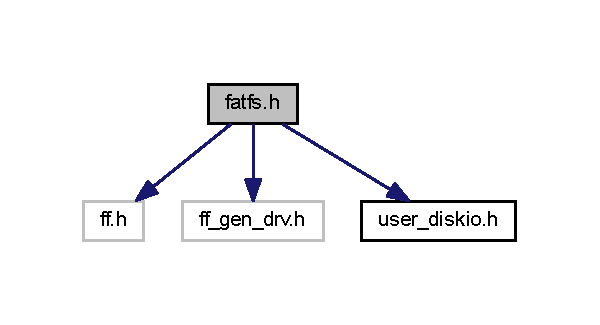
\includegraphics[width=288pt]{fatfs_8h__incl}
\end{center}
\end{figure}
This graph shows which files directly or indirectly include this file\+:\nopagebreak
\begin{figure}[H]
\begin{center}
\leavevmode
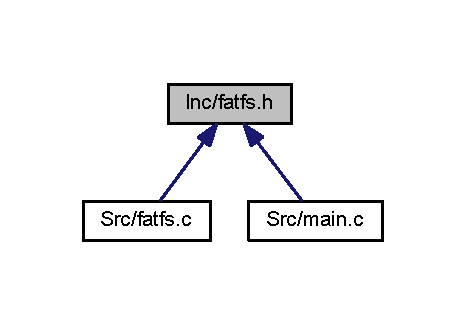
\includegraphics[width=224pt]{fatfs_8h__dep__incl}
\end{center}
\end{figure}
\subsection*{Functions}
\begin{DoxyCompactItemize}
\item 
void \mbox{\hyperlink{fatfs_8h_a3712bd1d3043334cf9343acc30bd2604}{M\+X\+\_\+\+F\+A\+T\+F\+S\+\_\+\+Init}} (void)
\end{DoxyCompactItemize}
\subsection*{Variables}
\begin{DoxyCompactItemize}
\item 
uint8\+\_\+t \mbox{\hyperlink{fatfs_8h_a424889af713d1b8afbb3e02352924792}{ret\+U\+S\+ER}}
\item 
char \mbox{\hyperlink{fatfs_8h_aba9c3aa07bcf2804dedcc0f7014a78ba}{U\+S\+E\+R\+Path}} \mbox{[}4\mbox{]}
\item 
F\+A\+T\+FS \mbox{\hyperlink{fatfs_8h_aeb1982f45f4eaf65071f64491c3c2c2f}{U\+S\+E\+R\+Fat\+FS}}
\item 
F\+IL \mbox{\hyperlink{fatfs_8h_a4e242af5cb4d75dbcb96a3213a3b1401}{U\+S\+E\+R\+File}}
\end{DoxyCompactItemize}


\subsection{Detailed Description}
Header for fatfs applications. 

This notice applies to any and all portions of this file that are not between comment pairs U\+S\+ER C\+O\+DE B\+E\+G\+IN and U\+S\+ER C\+O\+DE E\+ND. Other portions of this file, whether inserted by the user or by software development tools are owned by their respective copyright owners.

Copyright (c) 2018 S\+T\+Microelectronics International N.\+V. All rights reserved.

Redistribution and use in source and binary forms, with or without modification, are permitted, provided that the following conditions are met\+:


\begin{DoxyEnumerate}
\item Redistribution of source code must retain the above copyright notice, this list of conditions and the following disclaimer.
\item Redistributions in binary form must reproduce the above copyright notice, this list of conditions and the following disclaimer in the documentation and/or other materials provided with the distribution.
\item Neither the name of S\+T\+Microelectronics nor the names of other contributors to this software may be used to endorse or promote products derived from this software without specific written permission.
\item This software, including modifications and/or derivative works of this software, must execute solely and exclusively on microcontroller or microprocessor devices manufactured by or for S\+T\+Microelectronics.
\item Redistribution and use of this software other than as permitted under this license is void and will automatically terminate your rights under this license.
\end{DoxyEnumerate}

T\+H\+IS S\+O\+F\+T\+W\+A\+RE IS P\+R\+O\+V\+I\+D\+ED BY S\+T\+M\+I\+C\+R\+O\+E\+L\+E\+C\+T\+R\+O\+N\+I\+CS A\+ND C\+O\+N\+T\+R\+I\+B\+U\+T\+O\+RS \char`\"{}\+A\+S I\+S\char`\"{} A\+ND A\+NY E\+X\+P\+R\+E\+SS, I\+M\+P\+L\+I\+ED OR S\+T\+A\+T\+U\+T\+O\+RY W\+A\+R\+R\+A\+N\+T\+I\+ES, I\+N\+C\+L\+U\+D\+I\+NG, B\+UT N\+OT L\+I\+M\+I\+T\+ED TO, T\+HE I\+M\+P\+L\+I\+ED W\+A\+R\+R\+A\+N\+T\+I\+ES OF M\+E\+R\+C\+H\+A\+N\+T\+A\+B\+I\+L\+I\+TY, F\+I\+T\+N\+E\+SS F\+OR A P\+A\+R\+T\+I\+C\+U\+L\+AR P\+U\+R\+P\+O\+SE A\+ND N\+O\+N-\/\+I\+N\+F\+R\+I\+N\+G\+E\+M\+E\+NT OF T\+H\+I\+RD P\+A\+R\+TY I\+N\+T\+E\+L\+L\+E\+C\+T\+U\+AL P\+R\+O\+P\+E\+R\+TY R\+I\+G\+H\+TS A\+RE D\+I\+S\+C\+L\+A\+I\+M\+ED TO T\+HE F\+U\+L\+L\+E\+ST E\+X\+T\+E\+NT P\+E\+R\+M\+I\+T\+T\+ED BY L\+AW. IN NO E\+V\+E\+NT S\+H\+A\+LL S\+T\+M\+I\+C\+R\+O\+E\+L\+E\+C\+T\+R\+O\+N\+I\+CS OR C\+O\+N\+T\+R\+I\+B\+U\+T\+O\+RS BE L\+I\+A\+B\+LE F\+OR A\+NY D\+I\+R\+E\+CT, I\+N\+D\+I\+R\+E\+CT, I\+N\+C\+I\+D\+E\+N\+T\+AL, S\+P\+E\+C\+I\+AL, E\+X\+E\+M\+P\+L\+A\+RY, OR C\+O\+N\+S\+E\+Q\+U\+E\+N\+T\+I\+AL D\+A\+M\+A\+G\+ES (I\+N\+C\+L\+U\+D\+I\+NG, B\+UT N\+OT L\+I\+M\+I\+T\+ED TO, P\+R\+O\+C\+U\+R\+E\+M\+E\+NT OF S\+U\+B\+S\+T\+I\+T\+U\+TE G\+O\+O\+DS OR S\+E\+R\+V\+I\+C\+ES; L\+O\+SS OF U\+SE, D\+A\+TA, OR P\+R\+O\+F\+I\+TS; OR B\+U\+S\+I\+N\+E\+SS I\+N\+T\+E\+R\+R\+U\+P\+T\+I\+ON) H\+O\+W\+E\+V\+ER C\+A\+U\+S\+ED A\+ND ON A\+NY T\+H\+E\+O\+RY OF L\+I\+A\+B\+I\+L\+I\+TY, W\+H\+E\+T\+H\+ER IN C\+O\+N\+T\+R\+A\+CT, S\+T\+R\+I\+CT L\+I\+A\+B\+I\+L\+I\+TY, OR T\+O\+RT (I\+N\+C\+L\+U\+D\+I\+NG N\+E\+G\+L\+I\+G\+E\+N\+CE OR O\+T\+H\+E\+R\+W\+I\+SE) A\+R\+I\+S\+I\+NG IN A\+NY W\+AY O\+UT OF T\+HE U\+SE OF T\+H\+IS S\+O\+F\+T\+W\+A\+RE, E\+V\+EN IF A\+D\+V\+I\+S\+ED OF T\+HE P\+O\+S\+S\+I\+B\+I\+L\+I\+TY OF S\+U\+CH D\+A\+M\+A\+GE. 

\subsection{Function Documentation}
\mbox{\Hypertarget{fatfs_8h_a3712bd1d3043334cf9343acc30bd2604}\label{fatfs_8h_a3712bd1d3043334cf9343acc30bd2604}} 
\index{fatfs.\+h@{fatfs.\+h}!M\+X\+\_\+\+F\+A\+T\+F\+S\+\_\+\+Init@{M\+X\+\_\+\+F\+A\+T\+F\+S\+\_\+\+Init}}
\index{M\+X\+\_\+\+F\+A\+T\+F\+S\+\_\+\+Init@{M\+X\+\_\+\+F\+A\+T\+F\+S\+\_\+\+Init}!fatfs.\+h@{fatfs.\+h}}
\subsubsection{\texorpdfstring{M\+X\+\_\+\+F\+A\+T\+F\+S\+\_\+\+Init()}{MX\_FATFS\_Init()}}
{\footnotesize\ttfamily void M\+X\+\_\+\+F\+A\+T\+F\+S\+\_\+\+Init (\begin{DoxyParamCaption}\item[{void}]{ }\end{DoxyParamCaption})}



Definition at line 60 of file fatfs.\+c.

Here is the caller graph for this function\+:\nopagebreak
\begin{figure}[H]
\begin{center}
\leavevmode
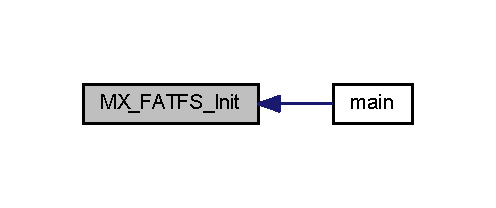
\includegraphics[width=238pt]{fatfs_8h_a3712bd1d3043334cf9343acc30bd2604_icgraph}
\end{center}
\end{figure}


\subsection{Variable Documentation}
\mbox{\Hypertarget{fatfs_8h_a424889af713d1b8afbb3e02352924792}\label{fatfs_8h_a424889af713d1b8afbb3e02352924792}} 
\index{fatfs.\+h@{fatfs.\+h}!ret\+U\+S\+ER@{ret\+U\+S\+ER}}
\index{ret\+U\+S\+ER@{ret\+U\+S\+ER}!fatfs.\+h@{fatfs.\+h}}
\subsubsection{\texorpdfstring{ret\+U\+S\+ER}{retUSER}}
{\footnotesize\ttfamily uint8\+\_\+t ret\+U\+S\+ER}



Definition at line 51 of file fatfs.\+c.

\mbox{\Hypertarget{fatfs_8h_aeb1982f45f4eaf65071f64491c3c2c2f}\label{fatfs_8h_aeb1982f45f4eaf65071f64491c3c2c2f}} 
\index{fatfs.\+h@{fatfs.\+h}!U\+S\+E\+R\+Fat\+FS@{U\+S\+E\+R\+Fat\+FS}}
\index{U\+S\+E\+R\+Fat\+FS@{U\+S\+E\+R\+Fat\+FS}!fatfs.\+h@{fatfs.\+h}}
\subsubsection{\texorpdfstring{U\+S\+E\+R\+Fat\+FS}{USERFatFS}}
{\footnotesize\ttfamily F\+A\+T\+FS U\+S\+E\+R\+Fat\+FS}



Definition at line 53 of file fatfs.\+c.

\mbox{\Hypertarget{fatfs_8h_a4e242af5cb4d75dbcb96a3213a3b1401}\label{fatfs_8h_a4e242af5cb4d75dbcb96a3213a3b1401}} 
\index{fatfs.\+h@{fatfs.\+h}!U\+S\+E\+R\+File@{U\+S\+E\+R\+File}}
\index{U\+S\+E\+R\+File@{U\+S\+E\+R\+File}!fatfs.\+h@{fatfs.\+h}}
\subsubsection{\texorpdfstring{U\+S\+E\+R\+File}{USERFile}}
{\footnotesize\ttfamily F\+IL U\+S\+E\+R\+File}



Definition at line 54 of file fatfs.\+c.

\mbox{\Hypertarget{fatfs_8h_aba9c3aa07bcf2804dedcc0f7014a78ba}\label{fatfs_8h_aba9c3aa07bcf2804dedcc0f7014a78ba}} 
\index{fatfs.\+h@{fatfs.\+h}!U\+S\+E\+R\+Path@{U\+S\+E\+R\+Path}}
\index{U\+S\+E\+R\+Path@{U\+S\+E\+R\+Path}!fatfs.\+h@{fatfs.\+h}}
\subsubsection{\texorpdfstring{U\+S\+E\+R\+Path}{USERPath}}
{\footnotesize\ttfamily char U\+S\+E\+R\+Path\mbox{[}4\mbox{]}}



Definition at line 52 of file fatfs.\+c.


\hypertarget{ffconf_8h}{}\section{Inc/ffconf.h File Reference}
\label{ffconf_8h}\index{Inc/ffconf.\+h@{Inc/ffconf.\+h}}
{\ttfamily \#include \char`\"{}stm32f4xx\+\_\+hal.\+h\char`\"{}}\newline
{\ttfamily \#include $<$stdlib.\+h$>$}\newline
Include dependency graph for ffconf.\+h\+:\nopagebreak
\begin{figure}[H]
\begin{center}
\leavevmode
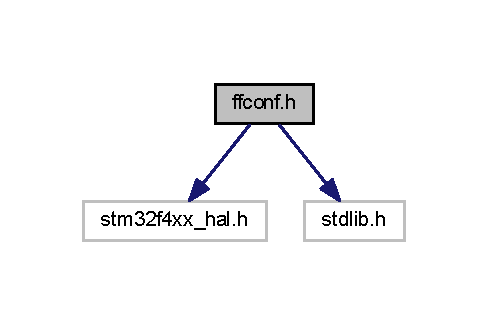
\includegraphics[width=234pt]{ffconf_8h__incl}
\end{center}
\end{figure}
\subsection*{Macros}
\begin{DoxyCompactItemize}
\item 
\#define \mbox{\hyperlink{ffconf_8h_a45082af332369ed49492446a2d4d4c5a}{\+\_\+\+F\+F\+C\+O\+NF}}~68300	/$\ast$ Revision ID $\ast$/
\item 
\#define \mbox{\hyperlink{ffconf_8h_afb8d35370cfe0c23832ac2d82e854ec6}{\+\_\+\+F\+S\+\_\+\+R\+E\+A\+D\+O\+N\+LY}}~0      /$\ast$ 0\+:Read/Write or 1\+:Read only $\ast$/
\item 
\#define \mbox{\hyperlink{ffconf_8h_abefed32e4f049538ff7d7101cd8e3643}{\+\_\+\+F\+S\+\_\+\+M\+I\+N\+I\+M\+I\+ZE}}~0      /$\ast$ 0 to 3 $\ast$/
\item 
\#define \mbox{\hyperlink{ffconf_8h_aaab0313f867bb008b64236239f5c2660}{\+\_\+\+U\+S\+E\+\_\+\+S\+T\+R\+F\+U\+NC}}~2      /$\ast$ 0\+:Disable or 1-\/2\+:Enable $\ast$/
\item 
\#define \mbox{\hyperlink{ffconf_8h_abf97f960987a4a2be3b876cc45612b06}{\+\_\+\+U\+S\+E\+\_\+\+F\+I\+ND}}~0
\item 
\#define \mbox{\hyperlink{ffconf_8h_a62cdce547af40f0c1599698ee151bbd7}{\+\_\+\+U\+S\+E\+\_\+\+M\+K\+FS}}~1
\item 
\#define \mbox{\hyperlink{ffconf_8h_a85f4bdb33729ebdaaf9edeec948ac0e7}{\+\_\+\+U\+S\+E\+\_\+\+F\+A\+S\+T\+S\+E\+EK}}~1
\item 
\#define \mbox{\hyperlink{ffconf_8h_a89e14a6d520a11044b87a947e83a5acb}{\+\_\+\+U\+S\+E\+\_\+\+E\+X\+P\+A\+ND}}~0
\item 
\#define \mbox{\hyperlink{ffconf_8h_adff028cbd80032c637fe1bb4e9b6fdfd}{\+\_\+\+U\+S\+E\+\_\+\+C\+H\+M\+OD}}~0
\item 
\#define \mbox{\hyperlink{ffconf_8h_a281a4fc4668e40fc896fc865f52f9421}{\+\_\+\+U\+S\+E\+\_\+\+L\+A\+B\+EL}}~0
\item 
\#define \mbox{\hyperlink{ffconf_8h_ae49b948c9a92ff7082b88bd36f63d988}{\+\_\+\+U\+S\+E\+\_\+\+F\+O\+R\+W\+A\+RD}}~0
\item 
\#define \mbox{\hyperlink{ffconf_8h_aaf9b5cee569d93f1ebe43ea70916569f}{\+\_\+\+C\+O\+D\+E\+\_\+\+P\+A\+GE}}~850
\item 
\#define \mbox{\hyperlink{ffconf_8h_ae471cce284bf1888f9e991f5a811fc11}{\+\_\+\+U\+S\+E\+\_\+\+L\+FN}}~0    /$\ast$ 0 to 3 $\ast$/
\item 
\#define \mbox{\hyperlink{ffconf_8h_a14e73a5c703a586c614b3e40b849f82c}{\+\_\+\+M\+A\+X\+\_\+\+L\+FN}}~255  /$\ast$ Maximum L\+FN length to handle (12 to 255) $\ast$/
\item 
\#define \mbox{\hyperlink{ffconf_8h_a8dd7e7f166bb146970b394d53cf01d80}{\+\_\+\+L\+F\+N\+\_\+\+U\+N\+I\+C\+O\+DE}}~0 /$\ast$ 0\+:A\+N\+SI/O\+EM or 1\+:Unicode $\ast$/
\item 
\#define \mbox{\hyperlink{ffconf_8h_a36a53af63e05351562e34f082eec3f33}{\+\_\+\+S\+T\+R\+F\+\_\+\+E\+N\+C\+O\+DE}}~3
\item 
\#define \mbox{\hyperlink{ffconf_8h_a52faf11025401372f71e9d81905b7af4}{\+\_\+\+F\+S\+\_\+\+R\+P\+A\+TH}}~0 /$\ast$ 0 to 2 $\ast$/
\item 
\#define \mbox{\hyperlink{ffconf_8h_a366da9a40c8ceb3103a6b72ca02b9969}{\+\_\+\+V\+O\+L\+U\+M\+ES}}~1
\item 
\#define \mbox{\hyperlink{ffconf_8h_ae89b13dba7638cb22b5587fcb335ffe3}{\+\_\+\+S\+T\+R\+\_\+\+V\+O\+L\+U\+M\+E\+\_\+\+ID}}~0	/$\ast$ 0\+:Use only 0-\/9 for drive ID, 1\+:Use strings for drive ID $\ast$/
\item 
\#define \mbox{\hyperlink{ffconf_8h_a75c97afb8b06935364e42e3ec3fdc6c4}{\+\_\+\+V\+O\+L\+U\+M\+E\+\_\+\+S\+T\+RS}}~\char`\"{}R\+AM\char`\"{},\char`\"{}N\+A\+ND\char`\"{},\char`\"{}CF\char`\"{},\char`\"{}S\+D1\char`\"{},\char`\"{}S\+D2\char`\"{},\char`\"{}U\+S\+B1\char`\"{},\char`\"{}U\+S\+B2\char`\"{},\char`\"{}U\+S\+B3\char`\"{}
\item 
\#define \mbox{\hyperlink{ffconf_8h_adc02609ba893fe8706a2f8af0e3a3bb5}{\+\_\+\+M\+U\+L\+T\+I\+\_\+\+P\+A\+R\+T\+I\+T\+I\+ON}}~0 /$\ast$ 0\+:Single partition, 1\+:Multiple partition $\ast$/
\item 
\#define \mbox{\hyperlink{ffconf_8h_ad03aa6d0e294709ae15898ee2c14dc3a}{\+\_\+\+M\+I\+N\+\_\+\+SS}}~512  /$\ast$ 512, 1024, 2048 or 4096 $\ast$/
\item 
\#define \mbox{\hyperlink{ffconf_8h_ac271b697378912f17132cb9c7d0de024}{\+\_\+\+M\+A\+X\+\_\+\+SS}}~512  /$\ast$ 512, 1024, 2048 or 4096 $\ast$/
\item 
\#define \mbox{\hyperlink{ffconf_8h_a1f93ee7e57bb9d1221f34bfe80e18a61}{\+\_\+\+U\+S\+E\+\_\+\+T\+R\+IM}}~0
\item 
\#define \mbox{\hyperlink{ffconf_8h_aaa0caa2085332d2febf0e392559ad138}{\+\_\+\+F\+S\+\_\+\+N\+O\+F\+S\+I\+N\+FO}}~0 /$\ast$ 0,1,2 or 3 $\ast$/
\item 
\#define \mbox{\hyperlink{ffconf_8h_aa21b30e70610594d3af3a28832b584f6}{\+\_\+\+F\+S\+\_\+\+T\+I\+NY}}~0      /$\ast$ 0\+:Normal or 1\+:Tiny $\ast$/
\item 
\#define \mbox{\hyperlink{ffconf_8h_a104309dc91be2af9375923ed7b03490e}{\+\_\+\+F\+S\+\_\+\+E\+X\+F\+AT}}~0
\item 
\#define \mbox{\hyperlink{ffconf_8h_a851cace7cfb7afdb4e892230cc075bbd}{\+\_\+\+F\+S\+\_\+\+N\+O\+R\+TC}}~0
\item 
\#define \mbox{\hyperlink{ffconf_8h_a47a493ecf767b65199e1425795f1d61d}{\+\_\+\+N\+O\+R\+T\+C\+\_\+\+M\+ON}}~6
\item 
\#define \mbox{\hyperlink{ffconf_8h_aa3cf28aa915cb9081fa1aa5b44858dd6}{\+\_\+\+N\+O\+R\+T\+C\+\_\+\+M\+D\+AY}}~4
\item 
\#define \mbox{\hyperlink{ffconf_8h_add853644b85a7633bb782dfddb51bda5}{\+\_\+\+N\+O\+R\+T\+C\+\_\+\+Y\+E\+AR}}~2015
\item 
\#define \mbox{\hyperlink{ffconf_8h_a01410fcb45c2d2d2c5692c56d4f0a481}{\+\_\+\+F\+S\+\_\+\+L\+O\+CK}}~2     /$\ast$ 0\+:Disable or $>$=1\+:Enable $\ast$/
\item 
\#define \mbox{\hyperlink{ffconf_8h_a4e07d7fcae4241b73eb5b70fab5f676d}{\+\_\+\+F\+S\+\_\+\+R\+E\+E\+N\+T\+R\+A\+NT}}~0  /$\ast$ 0\+:Disable or 1\+:Enable $\ast$/
\item 
\#define \mbox{\hyperlink{ffconf_8h_a526e3cac667f53cc9a48507873348e60}{\+\_\+\+F\+S\+\_\+\+T\+I\+M\+E\+O\+UT}}~1000 /$\ast$ Timeout period in unit of time ticks $\ast$/
\item 
\#define \mbox{\hyperlink{ffconf_8h_a9a3f0670343e51652dd12b18fa90a9eb}{\+\_\+\+S\+Y\+N\+C\+\_\+t}}~os\+Semaphore\+Id
\item 
\#define \mbox{\hyperlink{ffconf_8h_a1eee011a3d69ab8a3d199b985fe2ad36}{ff\+\_\+malloc}}~malloc
\item 
\#define \mbox{\hyperlink{ffconf_8h_ac7b5118894bfc43cc0d19f7290a7be0c}{ff\+\_\+free}}~free
\end{DoxyCompactItemize}


\subsection{Macro Definition Documentation}
\mbox{\Hypertarget{ffconf_8h_aaf9b5cee569d93f1ebe43ea70916569f}\label{ffconf_8h_aaf9b5cee569d93f1ebe43ea70916569f}} 
\index{ffconf.\+h@{ffconf.\+h}!\+\_\+\+C\+O\+D\+E\+\_\+\+P\+A\+GE@{\+\_\+\+C\+O\+D\+E\+\_\+\+P\+A\+GE}}
\index{\+\_\+\+C\+O\+D\+E\+\_\+\+P\+A\+GE@{\+\_\+\+C\+O\+D\+E\+\_\+\+P\+A\+GE}!ffconf.\+h@{ffconf.\+h}}
\subsubsection{\texorpdfstring{\+\_\+\+C\+O\+D\+E\+\_\+\+P\+A\+GE}{\_CODE\_PAGE}}
{\footnotesize\ttfamily \#define \+\_\+\+C\+O\+D\+E\+\_\+\+P\+A\+GE~850}



Definition at line 111 of file ffconf.\+h.

\mbox{\Hypertarget{ffconf_8h_a45082af332369ed49492446a2d4d4c5a}\label{ffconf_8h_a45082af332369ed49492446a2d4d4c5a}} 
\index{ffconf.\+h@{ffconf.\+h}!\+\_\+\+F\+F\+C\+O\+NF@{\+\_\+\+F\+F\+C\+O\+NF}}
\index{\+\_\+\+F\+F\+C\+O\+NF@{\+\_\+\+F\+F\+C\+O\+NF}!ffconf.\+h@{ffconf.\+h}}
\subsubsection{\texorpdfstring{\+\_\+\+F\+F\+C\+O\+NF}{\_FFCONF}}
{\footnotesize\ttfamily \#define \+\_\+\+F\+F\+C\+O\+NF~68300	/$\ast$ Revision ID $\ast$/}

Fat\+Fs -\/ Generic F\+AT file system module R0.\+12c (C)ChaN, 2017

This notice applies to any and all portions of this file that are not between comment pairs U\+S\+ER C\+O\+DE B\+E\+G\+IN and U\+S\+ER C\+O\+DE E\+ND. Other portions of this file, whether inserted by the user or by software development tools are owned by their respective copyright owners.

Copyright (c) 2018 S\+T\+Microelectronics International N.\+V. All rights reserved.

Redistribution and use in source and binary forms, with or without modification, are permitted, provided that the following conditions are met\+:


\begin{DoxyEnumerate}
\item Redistribution of source code must retain the above copyright notice, this list of conditions and the following disclaimer.
\item Redistributions in binary form must reproduce the above copyright notice, this list of conditions and the following disclaimer in the documentation and/or other materials provided with the distribution.
\item Neither the name of S\+T\+Microelectronics nor the names of other contributors to this software may be used to endorse or promote products derived from this software without specific written permission.
\item This software, including modifications and/or derivative works of this software, must execute solely and exclusively on microcontroller or microprocessor devices manufactured by or for S\+T\+Microelectronics.
\item Redistribution and use of this software other than as permitted under this license is void and will automatically terminate your rights under this license.
\end{DoxyEnumerate}

T\+H\+IS S\+O\+F\+T\+W\+A\+RE IS P\+R\+O\+V\+I\+D\+ED BY S\+T\+M\+I\+C\+R\+O\+E\+L\+E\+C\+T\+R\+O\+N\+I\+CS A\+ND C\+O\+N\+T\+R\+I\+B\+U\+T\+O\+RS \char`\"{}\+A\+S I\+S\char`\"{} A\+ND A\+NY E\+X\+P\+R\+E\+SS, I\+M\+P\+L\+I\+ED OR S\+T\+A\+T\+U\+T\+O\+RY W\+A\+R\+R\+A\+N\+T\+I\+ES, I\+N\+C\+L\+U\+D\+I\+NG, B\+UT N\+OT L\+I\+M\+I\+T\+ED TO, T\+HE I\+M\+P\+L\+I\+ED W\+A\+R\+R\+A\+N\+T\+I\+ES OF M\+E\+R\+C\+H\+A\+N\+T\+A\+B\+I\+L\+I\+TY, F\+I\+T\+N\+E\+SS F\+OR A P\+A\+R\+T\+I\+C\+U\+L\+AR P\+U\+R\+P\+O\+SE A\+ND N\+O\+N-\/\+I\+N\+F\+R\+I\+N\+G\+E\+M\+E\+NT OF T\+H\+I\+RD P\+A\+R\+TY I\+N\+T\+E\+L\+L\+E\+C\+T\+U\+AL P\+R\+O\+P\+E\+R\+TY R\+I\+G\+H\+TS A\+RE D\+I\+S\+C\+L\+A\+I\+M\+ED TO T\+HE F\+U\+L\+L\+E\+ST E\+X\+T\+E\+NT P\+E\+R\+M\+I\+T\+T\+ED BY L\+AW. IN NO E\+V\+E\+NT S\+H\+A\+LL S\+T\+M\+I\+C\+R\+O\+E\+L\+E\+C\+T\+R\+O\+N\+I\+CS OR C\+O\+N\+T\+R\+I\+B\+U\+T\+O\+RS BE L\+I\+A\+B\+LE F\+OR A\+NY D\+I\+R\+E\+CT, I\+N\+D\+I\+R\+E\+CT, I\+N\+C\+I\+D\+E\+N\+T\+AL, S\+P\+E\+C\+I\+AL, E\+X\+E\+M\+P\+L\+A\+RY, OR C\+O\+N\+S\+E\+Q\+U\+E\+N\+T\+I\+AL D\+A\+M\+A\+G\+ES (I\+N\+C\+L\+U\+D\+I\+NG, B\+UT N\+OT L\+I\+M\+I\+T\+ED TO, P\+R\+O\+C\+U\+R\+E\+M\+E\+NT OF S\+U\+B\+S\+T\+I\+T\+U\+TE G\+O\+O\+DS OR S\+E\+R\+V\+I\+C\+ES; L\+O\+SS OF U\+SE, D\+A\+TA, OR P\+R\+O\+F\+I\+TS; OR B\+U\+S\+I\+N\+E\+SS I\+N\+T\+E\+R\+R\+U\+P\+T\+I\+ON) H\+O\+W\+E\+V\+ER C\+A\+U\+S\+ED A\+ND ON A\+NY T\+H\+E\+O\+RY OF L\+I\+A\+B\+I\+L\+I\+TY, W\+H\+E\+T\+H\+ER IN C\+O\+N\+T\+R\+A\+CT, S\+T\+R\+I\+CT L\+I\+A\+B\+I\+L\+I\+TY, OR T\+O\+RT (I\+N\+C\+L\+U\+D\+I\+NG N\+E\+G\+L\+I\+G\+E\+N\+CE OR O\+T\+H\+E\+R\+W\+I\+SE) A\+R\+I\+S\+I\+NG IN A\+NY W\+AY O\+UT OF T\+HE U\+SE OF T\+H\+IS S\+O\+F\+T\+W\+A\+RE, E\+V\+EN IF A\+D\+V\+I\+S\+ED OF T\+HE P\+O\+S\+S\+I\+B\+I\+L\+I\+TY OF S\+U\+CH D\+A\+M\+A\+GE. 

Definition at line 49 of file ffconf.\+h.

\mbox{\Hypertarget{ffconf_8h_a104309dc91be2af9375923ed7b03490e}\label{ffconf_8h_a104309dc91be2af9375923ed7b03490e}} 
\index{ffconf.\+h@{ffconf.\+h}!\+\_\+\+F\+S\+\_\+\+E\+X\+F\+AT@{\+\_\+\+F\+S\+\_\+\+E\+X\+F\+AT}}
\index{\+\_\+\+F\+S\+\_\+\+E\+X\+F\+AT@{\+\_\+\+F\+S\+\_\+\+E\+X\+F\+AT}!ffconf.\+h@{ffconf.\+h}}
\subsubsection{\texorpdfstring{\+\_\+\+F\+S\+\_\+\+E\+X\+F\+AT}{\_FS\_EXFAT}}
{\footnotesize\ttfamily \#define \+\_\+\+F\+S\+\_\+\+E\+X\+F\+AT~0}



Definition at line 239 of file ffconf.\+h.

\mbox{\Hypertarget{ffconf_8h_a01410fcb45c2d2d2c5692c56d4f0a481}\label{ffconf_8h_a01410fcb45c2d2d2c5692c56d4f0a481}} 
\index{ffconf.\+h@{ffconf.\+h}!\+\_\+\+F\+S\+\_\+\+L\+O\+CK@{\+\_\+\+F\+S\+\_\+\+L\+O\+CK}}
\index{\+\_\+\+F\+S\+\_\+\+L\+O\+CK@{\+\_\+\+F\+S\+\_\+\+L\+O\+CK}!ffconf.\+h@{ffconf.\+h}}
\subsubsection{\texorpdfstring{\+\_\+\+F\+S\+\_\+\+L\+O\+CK}{\_FS\_LOCK}}
{\footnotesize\ttfamily \#define \+\_\+\+F\+S\+\_\+\+L\+O\+CK~2     /$\ast$ 0\+:Disable or $>$=1\+:Enable $\ast$/}



Definition at line 257 of file ffconf.\+h.

\mbox{\Hypertarget{ffconf_8h_abefed32e4f049538ff7d7101cd8e3643}\label{ffconf_8h_abefed32e4f049538ff7d7101cd8e3643}} 
\index{ffconf.\+h@{ffconf.\+h}!\+\_\+\+F\+S\+\_\+\+M\+I\+N\+I\+M\+I\+ZE@{\+\_\+\+F\+S\+\_\+\+M\+I\+N\+I\+M\+I\+ZE}}
\index{\+\_\+\+F\+S\+\_\+\+M\+I\+N\+I\+M\+I\+ZE@{\+\_\+\+F\+S\+\_\+\+M\+I\+N\+I\+M\+I\+ZE}!ffconf.\+h@{ffconf.\+h}}
\subsubsection{\texorpdfstring{\+\_\+\+F\+S\+\_\+\+M\+I\+N\+I\+M\+I\+ZE}{\_FS\_MINIMIZE}}
{\footnotesize\ttfamily \#define \+\_\+\+F\+S\+\_\+\+M\+I\+N\+I\+M\+I\+ZE~0      /$\ast$ 0 to 3 $\ast$/}



Definition at line 66 of file ffconf.\+h.

\mbox{\Hypertarget{ffconf_8h_aaa0caa2085332d2febf0e392559ad138}\label{ffconf_8h_aaa0caa2085332d2febf0e392559ad138}} 
\index{ffconf.\+h@{ffconf.\+h}!\+\_\+\+F\+S\+\_\+\+N\+O\+F\+S\+I\+N\+FO@{\+\_\+\+F\+S\+\_\+\+N\+O\+F\+S\+I\+N\+FO}}
\index{\+\_\+\+F\+S\+\_\+\+N\+O\+F\+S\+I\+N\+FO@{\+\_\+\+F\+S\+\_\+\+N\+O\+F\+S\+I\+N\+FO}!ffconf.\+h@{ffconf.\+h}}
\subsubsection{\texorpdfstring{\+\_\+\+F\+S\+\_\+\+N\+O\+F\+S\+I\+N\+FO}{\_FS\_NOFSINFO}}
{\footnotesize\ttfamily \#define \+\_\+\+F\+S\+\_\+\+N\+O\+F\+S\+I\+N\+FO~0 /$\ast$ 0,1,2 or 3 $\ast$/}



Definition at line 218 of file ffconf.\+h.

\mbox{\Hypertarget{ffconf_8h_a851cace7cfb7afdb4e892230cc075bbd}\label{ffconf_8h_a851cace7cfb7afdb4e892230cc075bbd}} 
\index{ffconf.\+h@{ffconf.\+h}!\+\_\+\+F\+S\+\_\+\+N\+O\+R\+TC@{\+\_\+\+F\+S\+\_\+\+N\+O\+R\+TC}}
\index{\+\_\+\+F\+S\+\_\+\+N\+O\+R\+TC@{\+\_\+\+F\+S\+\_\+\+N\+O\+R\+TC}!ffconf.\+h@{ffconf.\+h}}
\subsubsection{\texorpdfstring{\+\_\+\+F\+S\+\_\+\+N\+O\+R\+TC}{\_FS\_NORTC}}
{\footnotesize\ttfamily \#define \+\_\+\+F\+S\+\_\+\+N\+O\+R\+TC~0}



Definition at line 244 of file ffconf.\+h.

\mbox{\Hypertarget{ffconf_8h_afb8d35370cfe0c23832ac2d82e854ec6}\label{ffconf_8h_afb8d35370cfe0c23832ac2d82e854ec6}} 
\index{ffconf.\+h@{ffconf.\+h}!\+\_\+\+F\+S\+\_\+\+R\+E\+A\+D\+O\+N\+LY@{\+\_\+\+F\+S\+\_\+\+R\+E\+A\+D\+O\+N\+LY}}
\index{\+\_\+\+F\+S\+\_\+\+R\+E\+A\+D\+O\+N\+LY@{\+\_\+\+F\+S\+\_\+\+R\+E\+A\+D\+O\+N\+LY}!ffconf.\+h@{ffconf.\+h}}
\subsubsection{\texorpdfstring{\+\_\+\+F\+S\+\_\+\+R\+E\+A\+D\+O\+N\+LY}{\_FS\_READONLY}}
{\footnotesize\ttfamily \#define \+\_\+\+F\+S\+\_\+\+R\+E\+A\+D\+O\+N\+LY~0      /$\ast$ 0\+:Read/Write or 1\+:Read only $\ast$/}



Definition at line 60 of file ffconf.\+h.

\mbox{\Hypertarget{ffconf_8h_a4e07d7fcae4241b73eb5b70fab5f676d}\label{ffconf_8h_a4e07d7fcae4241b73eb5b70fab5f676d}} 
\index{ffconf.\+h@{ffconf.\+h}!\+\_\+\+F\+S\+\_\+\+R\+E\+E\+N\+T\+R\+A\+NT@{\+\_\+\+F\+S\+\_\+\+R\+E\+E\+N\+T\+R\+A\+NT}}
\index{\+\_\+\+F\+S\+\_\+\+R\+E\+E\+N\+T\+R\+A\+NT@{\+\_\+\+F\+S\+\_\+\+R\+E\+E\+N\+T\+R\+A\+NT}!ffconf.\+h@{ffconf.\+h}}
\subsubsection{\texorpdfstring{\+\_\+\+F\+S\+\_\+\+R\+E\+E\+N\+T\+R\+A\+NT}{\_FS\_REENTRANT}}
{\footnotesize\ttfamily \#define \+\_\+\+F\+S\+\_\+\+R\+E\+E\+N\+T\+R\+A\+NT~0  /$\ast$ 0\+:Disable or 1\+:Enable $\ast$/}



Definition at line 268 of file ffconf.\+h.

\mbox{\Hypertarget{ffconf_8h_a52faf11025401372f71e9d81905b7af4}\label{ffconf_8h_a52faf11025401372f71e9d81905b7af4}} 
\index{ffconf.\+h@{ffconf.\+h}!\+\_\+\+F\+S\+\_\+\+R\+P\+A\+TH@{\+\_\+\+F\+S\+\_\+\+R\+P\+A\+TH}}
\index{\+\_\+\+F\+S\+\_\+\+R\+P\+A\+TH@{\+\_\+\+F\+S\+\_\+\+R\+P\+A\+TH}!ffconf.\+h@{ffconf.\+h}}
\subsubsection{\texorpdfstring{\+\_\+\+F\+S\+\_\+\+R\+P\+A\+TH}{\_FS\_RPATH}}
{\footnotesize\ttfamily \#define \+\_\+\+F\+S\+\_\+\+R\+P\+A\+TH~0 /$\ast$ 0 to 2 $\ast$/}



Definition at line 172 of file ffconf.\+h.

\mbox{\Hypertarget{ffconf_8h_a526e3cac667f53cc9a48507873348e60}\label{ffconf_8h_a526e3cac667f53cc9a48507873348e60}} 
\index{ffconf.\+h@{ffconf.\+h}!\+\_\+\+F\+S\+\_\+\+T\+I\+M\+E\+O\+UT@{\+\_\+\+F\+S\+\_\+\+T\+I\+M\+E\+O\+UT}}
\index{\+\_\+\+F\+S\+\_\+\+T\+I\+M\+E\+O\+UT@{\+\_\+\+F\+S\+\_\+\+T\+I\+M\+E\+O\+UT}!ffconf.\+h@{ffconf.\+h}}
\subsubsection{\texorpdfstring{\+\_\+\+F\+S\+\_\+\+T\+I\+M\+E\+O\+UT}{\_FS\_TIMEOUT}}
{\footnotesize\ttfamily \#define \+\_\+\+F\+S\+\_\+\+T\+I\+M\+E\+O\+UT~1000 /$\ast$ Timeout period in unit of time ticks $\ast$/}



Definition at line 269 of file ffconf.\+h.

\mbox{\Hypertarget{ffconf_8h_aa21b30e70610594d3af3a28832b584f6}\label{ffconf_8h_aa21b30e70610594d3af3a28832b584f6}} 
\index{ffconf.\+h@{ffconf.\+h}!\+\_\+\+F\+S\+\_\+\+T\+I\+NY@{\+\_\+\+F\+S\+\_\+\+T\+I\+NY}}
\index{\+\_\+\+F\+S\+\_\+\+T\+I\+NY@{\+\_\+\+F\+S\+\_\+\+T\+I\+NY}!ffconf.\+h@{ffconf.\+h}}
\subsubsection{\texorpdfstring{\+\_\+\+F\+S\+\_\+\+T\+I\+NY}{\_FS\_TINY}}
{\footnotesize\ttfamily \#define \+\_\+\+F\+S\+\_\+\+T\+I\+NY~0      /$\ast$ 0\+:Normal or 1\+:Tiny $\ast$/}



Definition at line 233 of file ffconf.\+h.

\mbox{\Hypertarget{ffconf_8h_a8dd7e7f166bb146970b394d53cf01d80}\label{ffconf_8h_a8dd7e7f166bb146970b394d53cf01d80}} 
\index{ffconf.\+h@{ffconf.\+h}!\+\_\+\+L\+F\+N\+\_\+\+U\+N\+I\+C\+O\+DE@{\+\_\+\+L\+F\+N\+\_\+\+U\+N\+I\+C\+O\+DE}}
\index{\+\_\+\+L\+F\+N\+\_\+\+U\+N\+I\+C\+O\+DE@{\+\_\+\+L\+F\+N\+\_\+\+U\+N\+I\+C\+O\+DE}!ffconf.\+h@{ffconf.\+h}}
\subsubsection{\texorpdfstring{\+\_\+\+L\+F\+N\+\_\+\+U\+N\+I\+C\+O\+DE}{\_LFN\_UNICODE}}
{\footnotesize\ttfamily \#define \+\_\+\+L\+F\+N\+\_\+\+U\+N\+I\+C\+O\+DE~0 /$\ast$ 0\+:A\+N\+SI/O\+EM or 1\+:Unicode $\ast$/}



Definition at line 156 of file ffconf.\+h.

\mbox{\Hypertarget{ffconf_8h_a14e73a5c703a586c614b3e40b849f82c}\label{ffconf_8h_a14e73a5c703a586c614b3e40b849f82c}} 
\index{ffconf.\+h@{ffconf.\+h}!\+\_\+\+M\+A\+X\+\_\+\+L\+FN@{\+\_\+\+M\+A\+X\+\_\+\+L\+FN}}
\index{\+\_\+\+M\+A\+X\+\_\+\+L\+FN@{\+\_\+\+M\+A\+X\+\_\+\+L\+FN}!ffconf.\+h@{ffconf.\+h}}
\subsubsection{\texorpdfstring{\+\_\+\+M\+A\+X\+\_\+\+L\+FN}{\_MAX\_LFN}}
{\footnotesize\ttfamily \#define \+\_\+\+M\+A\+X\+\_\+\+L\+FN~255  /$\ast$ Maximum L\+FN length to handle (12 to 255) $\ast$/}



Definition at line 140 of file ffconf.\+h.

\mbox{\Hypertarget{ffconf_8h_ac271b697378912f17132cb9c7d0de024}\label{ffconf_8h_ac271b697378912f17132cb9c7d0de024}} 
\index{ffconf.\+h@{ffconf.\+h}!\+\_\+\+M\+A\+X\+\_\+\+SS@{\+\_\+\+M\+A\+X\+\_\+\+SS}}
\index{\+\_\+\+M\+A\+X\+\_\+\+SS@{\+\_\+\+M\+A\+X\+\_\+\+SS}!ffconf.\+h@{ffconf.\+h}}
\subsubsection{\texorpdfstring{\+\_\+\+M\+A\+X\+\_\+\+SS}{\_MAX\_SS}}
{\footnotesize\ttfamily \#define \+\_\+\+M\+A\+X\+\_\+\+SS~512  /$\ast$ 512, 1024, 2048 or 4096 $\ast$/}



Definition at line 205 of file ffconf.\+h.

\mbox{\Hypertarget{ffconf_8h_ad03aa6d0e294709ae15898ee2c14dc3a}\label{ffconf_8h_ad03aa6d0e294709ae15898ee2c14dc3a}} 
\index{ffconf.\+h@{ffconf.\+h}!\+\_\+\+M\+I\+N\+\_\+\+SS@{\+\_\+\+M\+I\+N\+\_\+\+SS}}
\index{\+\_\+\+M\+I\+N\+\_\+\+SS@{\+\_\+\+M\+I\+N\+\_\+\+SS}!ffconf.\+h@{ffconf.\+h}}
\subsubsection{\texorpdfstring{\+\_\+\+M\+I\+N\+\_\+\+SS}{\_MIN\_SS}}
{\footnotesize\ttfamily \#define \+\_\+\+M\+I\+N\+\_\+\+SS~512  /$\ast$ 512, 1024, 2048 or 4096 $\ast$/}



Definition at line 204 of file ffconf.\+h.

\mbox{\Hypertarget{ffconf_8h_adc02609ba893fe8706a2f8af0e3a3bb5}\label{ffconf_8h_adc02609ba893fe8706a2f8af0e3a3bb5}} 
\index{ffconf.\+h@{ffconf.\+h}!\+\_\+\+M\+U\+L\+T\+I\+\_\+\+P\+A\+R\+T\+I\+T\+I\+ON@{\+\_\+\+M\+U\+L\+T\+I\+\_\+\+P\+A\+R\+T\+I\+T\+I\+ON}}
\index{\+\_\+\+M\+U\+L\+T\+I\+\_\+\+P\+A\+R\+T\+I\+T\+I\+ON@{\+\_\+\+M\+U\+L\+T\+I\+\_\+\+P\+A\+R\+T\+I\+T\+I\+ON}!ffconf.\+h@{ffconf.\+h}}
\subsubsection{\texorpdfstring{\+\_\+\+M\+U\+L\+T\+I\+\_\+\+P\+A\+R\+T\+I\+T\+I\+ON}{\_MULTI\_PARTITION}}
{\footnotesize\ttfamily \#define \+\_\+\+M\+U\+L\+T\+I\+\_\+\+P\+A\+R\+T\+I\+T\+I\+ON~0 /$\ast$ 0\+:Single partition, 1\+:Multiple partition $\ast$/}



Definition at line 197 of file ffconf.\+h.

\mbox{\Hypertarget{ffconf_8h_aa3cf28aa915cb9081fa1aa5b44858dd6}\label{ffconf_8h_aa3cf28aa915cb9081fa1aa5b44858dd6}} 
\index{ffconf.\+h@{ffconf.\+h}!\+\_\+\+N\+O\+R\+T\+C\+\_\+\+M\+D\+AY@{\+\_\+\+N\+O\+R\+T\+C\+\_\+\+M\+D\+AY}}
\index{\+\_\+\+N\+O\+R\+T\+C\+\_\+\+M\+D\+AY@{\+\_\+\+N\+O\+R\+T\+C\+\_\+\+M\+D\+AY}!ffconf.\+h@{ffconf.\+h}}
\subsubsection{\texorpdfstring{\+\_\+\+N\+O\+R\+T\+C\+\_\+\+M\+D\+AY}{\_NORTC\_MDAY}}
{\footnotesize\ttfamily \#define \+\_\+\+N\+O\+R\+T\+C\+\_\+\+M\+D\+AY~4}



Definition at line 246 of file ffconf.\+h.

\mbox{\Hypertarget{ffconf_8h_a47a493ecf767b65199e1425795f1d61d}\label{ffconf_8h_a47a493ecf767b65199e1425795f1d61d}} 
\index{ffconf.\+h@{ffconf.\+h}!\+\_\+\+N\+O\+R\+T\+C\+\_\+\+M\+ON@{\+\_\+\+N\+O\+R\+T\+C\+\_\+\+M\+ON}}
\index{\+\_\+\+N\+O\+R\+T\+C\+\_\+\+M\+ON@{\+\_\+\+N\+O\+R\+T\+C\+\_\+\+M\+ON}!ffconf.\+h@{ffconf.\+h}}
\subsubsection{\texorpdfstring{\+\_\+\+N\+O\+R\+T\+C\+\_\+\+M\+ON}{\_NORTC\_MON}}
{\footnotesize\ttfamily \#define \+\_\+\+N\+O\+R\+T\+C\+\_\+\+M\+ON~6}



Definition at line 245 of file ffconf.\+h.

\mbox{\Hypertarget{ffconf_8h_add853644b85a7633bb782dfddb51bda5}\label{ffconf_8h_add853644b85a7633bb782dfddb51bda5}} 
\index{ffconf.\+h@{ffconf.\+h}!\+\_\+\+N\+O\+R\+T\+C\+\_\+\+Y\+E\+AR@{\+\_\+\+N\+O\+R\+T\+C\+\_\+\+Y\+E\+AR}}
\index{\+\_\+\+N\+O\+R\+T\+C\+\_\+\+Y\+E\+AR@{\+\_\+\+N\+O\+R\+T\+C\+\_\+\+Y\+E\+AR}!ffconf.\+h@{ffconf.\+h}}
\subsubsection{\texorpdfstring{\+\_\+\+N\+O\+R\+T\+C\+\_\+\+Y\+E\+AR}{\_NORTC\_YEAR}}
{\footnotesize\ttfamily \#define \+\_\+\+N\+O\+R\+T\+C\+\_\+\+Y\+E\+AR~2015}



Definition at line 247 of file ffconf.\+h.

\mbox{\Hypertarget{ffconf_8h_ae89b13dba7638cb22b5587fcb335ffe3}\label{ffconf_8h_ae89b13dba7638cb22b5587fcb335ffe3}} 
\index{ffconf.\+h@{ffconf.\+h}!\+\_\+\+S\+T\+R\+\_\+\+V\+O\+L\+U\+M\+E\+\_\+\+ID@{\+\_\+\+S\+T\+R\+\_\+\+V\+O\+L\+U\+M\+E\+\_\+\+ID}}
\index{\+\_\+\+S\+T\+R\+\_\+\+V\+O\+L\+U\+M\+E\+\_\+\+ID@{\+\_\+\+S\+T\+R\+\_\+\+V\+O\+L\+U\+M\+E\+\_\+\+ID}!ffconf.\+h@{ffconf.\+h}}
\subsubsection{\texorpdfstring{\+\_\+\+S\+T\+R\+\_\+\+V\+O\+L\+U\+M\+E\+\_\+\+ID}{\_STR\_VOLUME\_ID}}
{\footnotesize\ttfamily \#define \+\_\+\+S\+T\+R\+\_\+\+V\+O\+L\+U\+M\+E\+\_\+\+ID~0	/$\ast$ 0\+:Use only 0-\/9 for drive ID, 1\+:Use strings for drive ID $\ast$/}



Definition at line 188 of file ffconf.\+h.

\mbox{\Hypertarget{ffconf_8h_a36a53af63e05351562e34f082eec3f33}\label{ffconf_8h_a36a53af63e05351562e34f082eec3f33}} 
\index{ffconf.\+h@{ffconf.\+h}!\+\_\+\+S\+T\+R\+F\+\_\+\+E\+N\+C\+O\+DE@{\+\_\+\+S\+T\+R\+F\+\_\+\+E\+N\+C\+O\+DE}}
\index{\+\_\+\+S\+T\+R\+F\+\_\+\+E\+N\+C\+O\+DE@{\+\_\+\+S\+T\+R\+F\+\_\+\+E\+N\+C\+O\+DE}!ffconf.\+h@{ffconf.\+h}}
\subsubsection{\texorpdfstring{\+\_\+\+S\+T\+R\+F\+\_\+\+E\+N\+C\+O\+DE}{\_STRF\_ENCODE}}
{\footnotesize\ttfamily \#define \+\_\+\+S\+T\+R\+F\+\_\+\+E\+N\+C\+O\+DE~3}



Definition at line 161 of file ffconf.\+h.

\mbox{\Hypertarget{ffconf_8h_a9a3f0670343e51652dd12b18fa90a9eb}\label{ffconf_8h_a9a3f0670343e51652dd12b18fa90a9eb}} 
\index{ffconf.\+h@{ffconf.\+h}!\+\_\+\+S\+Y\+N\+C\+\_\+t@{\+\_\+\+S\+Y\+N\+C\+\_\+t}}
\index{\+\_\+\+S\+Y\+N\+C\+\_\+t@{\+\_\+\+S\+Y\+N\+C\+\_\+t}!ffconf.\+h@{ffconf.\+h}}
\subsubsection{\texorpdfstring{\+\_\+\+S\+Y\+N\+C\+\_\+t}{\_SYNC\_t}}
{\footnotesize\ttfamily \#define \+\_\+\+S\+Y\+N\+C\+\_\+t~os\+Semaphore\+Id}



Definition at line 270 of file ffconf.\+h.

\mbox{\Hypertarget{ffconf_8h_adff028cbd80032c637fe1bb4e9b6fdfd}\label{ffconf_8h_adff028cbd80032c637fe1bb4e9b6fdfd}} 
\index{ffconf.\+h@{ffconf.\+h}!\+\_\+\+U\+S\+E\+\_\+\+C\+H\+M\+OD@{\+\_\+\+U\+S\+E\+\_\+\+C\+H\+M\+OD}}
\index{\+\_\+\+U\+S\+E\+\_\+\+C\+H\+M\+OD@{\+\_\+\+U\+S\+E\+\_\+\+C\+H\+M\+OD}!ffconf.\+h@{ffconf.\+h}}
\subsubsection{\texorpdfstring{\+\_\+\+U\+S\+E\+\_\+\+C\+H\+M\+OD}{\_USE\_CHMOD}}
{\footnotesize\ttfamily \#define \+\_\+\+U\+S\+E\+\_\+\+C\+H\+M\+OD~0}



Definition at line 96 of file ffconf.\+h.

\mbox{\Hypertarget{ffconf_8h_a89e14a6d520a11044b87a947e83a5acb}\label{ffconf_8h_a89e14a6d520a11044b87a947e83a5acb}} 
\index{ffconf.\+h@{ffconf.\+h}!\+\_\+\+U\+S\+E\+\_\+\+E\+X\+P\+A\+ND@{\+\_\+\+U\+S\+E\+\_\+\+E\+X\+P\+A\+ND}}
\index{\+\_\+\+U\+S\+E\+\_\+\+E\+X\+P\+A\+ND@{\+\_\+\+U\+S\+E\+\_\+\+E\+X\+P\+A\+ND}!ffconf.\+h@{ffconf.\+h}}
\subsubsection{\texorpdfstring{\+\_\+\+U\+S\+E\+\_\+\+E\+X\+P\+A\+ND}{\_USE\_EXPAND}}
{\footnotesize\ttfamily \#define \+\_\+\+U\+S\+E\+\_\+\+E\+X\+P\+A\+ND~0}



Definition at line 93 of file ffconf.\+h.

\mbox{\Hypertarget{ffconf_8h_a85f4bdb33729ebdaaf9edeec948ac0e7}\label{ffconf_8h_a85f4bdb33729ebdaaf9edeec948ac0e7}} 
\index{ffconf.\+h@{ffconf.\+h}!\+\_\+\+U\+S\+E\+\_\+\+F\+A\+S\+T\+S\+E\+EK@{\+\_\+\+U\+S\+E\+\_\+\+F\+A\+S\+T\+S\+E\+EK}}
\index{\+\_\+\+U\+S\+E\+\_\+\+F\+A\+S\+T\+S\+E\+EK@{\+\_\+\+U\+S\+E\+\_\+\+F\+A\+S\+T\+S\+E\+EK}!ffconf.\+h@{ffconf.\+h}}
\subsubsection{\texorpdfstring{\+\_\+\+U\+S\+E\+\_\+\+F\+A\+S\+T\+S\+E\+EK}{\_USE\_FASTSEEK}}
{\footnotesize\ttfamily \#define \+\_\+\+U\+S\+E\+\_\+\+F\+A\+S\+T\+S\+E\+EK~1}



Definition at line 90 of file ffconf.\+h.

\mbox{\Hypertarget{ffconf_8h_abf97f960987a4a2be3b876cc45612b06}\label{ffconf_8h_abf97f960987a4a2be3b876cc45612b06}} 
\index{ffconf.\+h@{ffconf.\+h}!\+\_\+\+U\+S\+E\+\_\+\+F\+I\+ND@{\+\_\+\+U\+S\+E\+\_\+\+F\+I\+ND}}
\index{\+\_\+\+U\+S\+E\+\_\+\+F\+I\+ND@{\+\_\+\+U\+S\+E\+\_\+\+F\+I\+ND}!ffconf.\+h@{ffconf.\+h}}
\subsubsection{\texorpdfstring{\+\_\+\+U\+S\+E\+\_\+\+F\+I\+ND}{\_USE\_FIND}}
{\footnotesize\ttfamily \#define \+\_\+\+U\+S\+E\+\_\+\+F\+I\+ND~0}



Definition at line 83 of file ffconf.\+h.

\mbox{\Hypertarget{ffconf_8h_ae49b948c9a92ff7082b88bd36f63d988}\label{ffconf_8h_ae49b948c9a92ff7082b88bd36f63d988}} 
\index{ffconf.\+h@{ffconf.\+h}!\+\_\+\+U\+S\+E\+\_\+\+F\+O\+R\+W\+A\+RD@{\+\_\+\+U\+S\+E\+\_\+\+F\+O\+R\+W\+A\+RD}}
\index{\+\_\+\+U\+S\+E\+\_\+\+F\+O\+R\+W\+A\+RD@{\+\_\+\+U\+S\+E\+\_\+\+F\+O\+R\+W\+A\+RD}!ffconf.\+h@{ffconf.\+h}}
\subsubsection{\texorpdfstring{\+\_\+\+U\+S\+E\+\_\+\+F\+O\+R\+W\+A\+RD}{\_USE\_FORWARD}}
{\footnotesize\ttfamily \#define \+\_\+\+U\+S\+E\+\_\+\+F\+O\+R\+W\+A\+RD~0}



Definition at line 104 of file ffconf.\+h.

\mbox{\Hypertarget{ffconf_8h_a281a4fc4668e40fc896fc865f52f9421}\label{ffconf_8h_a281a4fc4668e40fc896fc865f52f9421}} 
\index{ffconf.\+h@{ffconf.\+h}!\+\_\+\+U\+S\+E\+\_\+\+L\+A\+B\+EL@{\+\_\+\+U\+S\+E\+\_\+\+L\+A\+B\+EL}}
\index{\+\_\+\+U\+S\+E\+\_\+\+L\+A\+B\+EL@{\+\_\+\+U\+S\+E\+\_\+\+L\+A\+B\+EL}!ffconf.\+h@{ffconf.\+h}}
\subsubsection{\texorpdfstring{\+\_\+\+U\+S\+E\+\_\+\+L\+A\+B\+EL}{\_USE\_LABEL}}
{\footnotesize\ttfamily \#define \+\_\+\+U\+S\+E\+\_\+\+L\+A\+B\+EL~0}



Definition at line 100 of file ffconf.\+h.

\mbox{\Hypertarget{ffconf_8h_ae471cce284bf1888f9e991f5a811fc11}\label{ffconf_8h_ae471cce284bf1888f9e991f5a811fc11}} 
\index{ffconf.\+h@{ffconf.\+h}!\+\_\+\+U\+S\+E\+\_\+\+L\+FN@{\+\_\+\+U\+S\+E\+\_\+\+L\+FN}}
\index{\+\_\+\+U\+S\+E\+\_\+\+L\+FN@{\+\_\+\+U\+S\+E\+\_\+\+L\+FN}!ffconf.\+h@{ffconf.\+h}}
\subsubsection{\texorpdfstring{\+\_\+\+U\+S\+E\+\_\+\+L\+FN}{\_USE\_LFN}}
{\footnotesize\ttfamily \#define \+\_\+\+U\+S\+E\+\_\+\+L\+FN~0    /$\ast$ 0 to 3 $\ast$/}



Definition at line 139 of file ffconf.\+h.

\mbox{\Hypertarget{ffconf_8h_a62cdce547af40f0c1599698ee151bbd7}\label{ffconf_8h_a62cdce547af40f0c1599698ee151bbd7}} 
\index{ffconf.\+h@{ffconf.\+h}!\+\_\+\+U\+S\+E\+\_\+\+M\+K\+FS@{\+\_\+\+U\+S\+E\+\_\+\+M\+K\+FS}}
\index{\+\_\+\+U\+S\+E\+\_\+\+M\+K\+FS@{\+\_\+\+U\+S\+E\+\_\+\+M\+K\+FS}!ffconf.\+h@{ffconf.\+h}}
\subsubsection{\texorpdfstring{\+\_\+\+U\+S\+E\+\_\+\+M\+K\+FS}{\_USE\_MKFS}}
{\footnotesize\ttfamily \#define \+\_\+\+U\+S\+E\+\_\+\+M\+K\+FS~1}



Definition at line 87 of file ffconf.\+h.

\mbox{\Hypertarget{ffconf_8h_aaab0313f867bb008b64236239f5c2660}\label{ffconf_8h_aaab0313f867bb008b64236239f5c2660}} 
\index{ffconf.\+h@{ffconf.\+h}!\+\_\+\+U\+S\+E\+\_\+\+S\+T\+R\+F\+U\+NC@{\+\_\+\+U\+S\+E\+\_\+\+S\+T\+R\+F\+U\+NC}}
\index{\+\_\+\+U\+S\+E\+\_\+\+S\+T\+R\+F\+U\+NC@{\+\_\+\+U\+S\+E\+\_\+\+S\+T\+R\+F\+U\+NC}!ffconf.\+h@{ffconf.\+h}}
\subsubsection{\texorpdfstring{\+\_\+\+U\+S\+E\+\_\+\+S\+T\+R\+F\+U\+NC}{\_USE\_STRFUNC}}
{\footnotesize\ttfamily \#define \+\_\+\+U\+S\+E\+\_\+\+S\+T\+R\+F\+U\+NC~2      /$\ast$ 0\+:Disable or 1-\/2\+:Enable $\ast$/}



Definition at line 75 of file ffconf.\+h.

\mbox{\Hypertarget{ffconf_8h_a1f93ee7e57bb9d1221f34bfe80e18a61}\label{ffconf_8h_a1f93ee7e57bb9d1221f34bfe80e18a61}} 
\index{ffconf.\+h@{ffconf.\+h}!\+\_\+\+U\+S\+E\+\_\+\+T\+R\+IM@{\+\_\+\+U\+S\+E\+\_\+\+T\+R\+IM}}
\index{\+\_\+\+U\+S\+E\+\_\+\+T\+R\+IM@{\+\_\+\+U\+S\+E\+\_\+\+T\+R\+IM}!ffconf.\+h@{ffconf.\+h}}
\subsubsection{\texorpdfstring{\+\_\+\+U\+S\+E\+\_\+\+T\+R\+IM}{\_USE\_TRIM}}
{\footnotesize\ttfamily \#define \+\_\+\+U\+S\+E\+\_\+\+T\+R\+IM~0}



Definition at line 213 of file ffconf.\+h.

\mbox{\Hypertarget{ffconf_8h_a75c97afb8b06935364e42e3ec3fdc6c4}\label{ffconf_8h_a75c97afb8b06935364e42e3ec3fdc6c4}} 
\index{ffconf.\+h@{ffconf.\+h}!\+\_\+\+V\+O\+L\+U\+M\+E\+\_\+\+S\+T\+RS@{\+\_\+\+V\+O\+L\+U\+M\+E\+\_\+\+S\+T\+RS}}
\index{\+\_\+\+V\+O\+L\+U\+M\+E\+\_\+\+S\+T\+RS@{\+\_\+\+V\+O\+L\+U\+M\+E\+\_\+\+S\+T\+RS}!ffconf.\+h@{ffconf.\+h}}
\subsubsection{\texorpdfstring{\+\_\+\+V\+O\+L\+U\+M\+E\+\_\+\+S\+T\+RS}{\_VOLUME\_STRS}}
{\footnotesize\ttfamily \#define \+\_\+\+V\+O\+L\+U\+M\+E\+\_\+\+S\+T\+RS~\char`\"{}R\+AM\char`\"{},\char`\"{}N\+A\+ND\char`\"{},\char`\"{}CF\char`\"{},\char`\"{}S\+D1\char`\"{},\char`\"{}S\+D2\char`\"{},\char`\"{}U\+S\+B1\char`\"{},\char`\"{}U\+S\+B2\char`\"{},\char`\"{}U\+S\+B3\char`\"{}}



Definition at line 189 of file ffconf.\+h.

\mbox{\Hypertarget{ffconf_8h_a366da9a40c8ceb3103a6b72ca02b9969}\label{ffconf_8h_a366da9a40c8ceb3103a6b72ca02b9969}} 
\index{ffconf.\+h@{ffconf.\+h}!\+\_\+\+V\+O\+L\+U\+M\+ES@{\+\_\+\+V\+O\+L\+U\+M\+ES}}
\index{\+\_\+\+V\+O\+L\+U\+M\+ES@{\+\_\+\+V\+O\+L\+U\+M\+ES}!ffconf.\+h@{ffconf.\+h}}
\subsubsection{\texorpdfstring{\+\_\+\+V\+O\+L\+U\+M\+ES}{\_VOLUMES}}
{\footnotesize\ttfamily \#define \+\_\+\+V\+O\+L\+U\+M\+ES~1}



Definition at line 184 of file ffconf.\+h.

\mbox{\Hypertarget{ffconf_8h_ac7b5118894bfc43cc0d19f7290a7be0c}\label{ffconf_8h_ac7b5118894bfc43cc0d19f7290a7be0c}} 
\index{ffconf.\+h@{ffconf.\+h}!ff\+\_\+free@{ff\+\_\+free}}
\index{ff\+\_\+free@{ff\+\_\+free}!ffconf.\+h@{ffconf.\+h}}
\subsubsection{\texorpdfstring{ff\+\_\+free}{ff\_free}}
{\footnotesize\ttfamily \#define ff\+\_\+free~free}



Definition at line 292 of file ffconf.\+h.

\mbox{\Hypertarget{ffconf_8h_a1eee011a3d69ab8a3d199b985fe2ad36}\label{ffconf_8h_a1eee011a3d69ab8a3d199b985fe2ad36}} 
\index{ffconf.\+h@{ffconf.\+h}!ff\+\_\+malloc@{ff\+\_\+malloc}}
\index{ff\+\_\+malloc@{ff\+\_\+malloc}!ffconf.\+h@{ffconf.\+h}}
\subsubsection{\texorpdfstring{ff\+\_\+malloc}{ff\_malloc}}
{\footnotesize\ttfamily \#define ff\+\_\+malloc~malloc}



Definition at line 291 of file ffconf.\+h.


\hypertarget{gpio_8h}{}\section{Inc/gpio.h File Reference}
\label{gpio_8h}\index{Inc/gpio.\+h@{Inc/gpio.\+h}}
{\ttfamily \#include \char`\"{}stm32f4xx\+\_\+hal.\+h\char`\"{}}\newline
{\ttfamily \#include \char`\"{}main.\+h\char`\"{}}\newline
Include dependency graph for gpio.\+h\+:\nopagebreak
\begin{figure}[H]
\begin{center}
\leavevmode
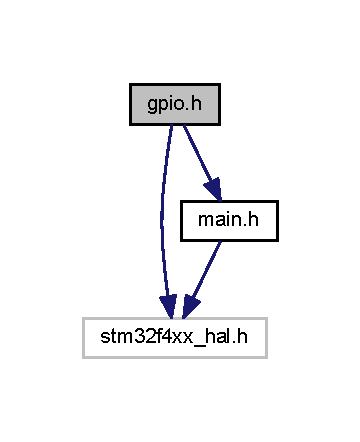
\includegraphics[width=173pt]{gpio_8h__incl}
\end{center}
\end{figure}
This graph shows which files directly or indirectly include this file\+:\nopagebreak
\begin{figure}[H]
\begin{center}
\leavevmode
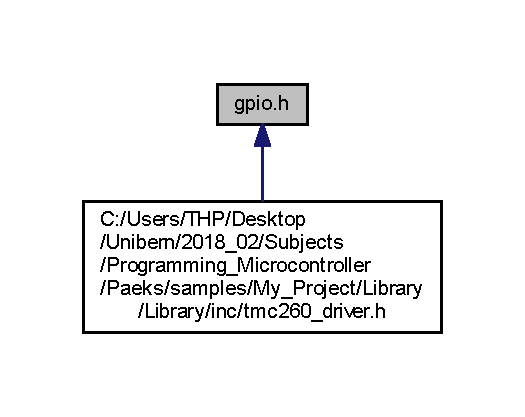
\includegraphics[width=350pt]{gpio_8h__dep__incl}
\end{center}
\end{figure}
\subsection*{Functions}
\begin{DoxyCompactItemize}
\item 
void \mbox{\hyperlink{gpio_8h_ac724e431d2af879252de35615be2bdea}{M\+X\+\_\+\+G\+P\+I\+O\+\_\+\+Init}} (void)
\end{DoxyCompactItemize}


\subsection{Function Documentation}
\mbox{\Hypertarget{gpio_8h_ac724e431d2af879252de35615be2bdea}\label{gpio_8h_ac724e431d2af879252de35615be2bdea}} 
\index{gpio.\+h@{gpio.\+h}!M\+X\+\_\+\+G\+P\+I\+O\+\_\+\+Init@{M\+X\+\_\+\+G\+P\+I\+O\+\_\+\+Init}}
\index{M\+X\+\_\+\+G\+P\+I\+O\+\_\+\+Init@{M\+X\+\_\+\+G\+P\+I\+O\+\_\+\+Init}!gpio.\+h@{gpio.\+h}}
\subsubsection{\texorpdfstring{M\+X\+\_\+\+G\+P\+I\+O\+\_\+\+Init()}{MX\_GPIO\_Init()}}
{\footnotesize\ttfamily void M\+X\+\_\+\+G\+P\+I\+O\+\_\+\+Init (\begin{DoxyParamCaption}\item[{void}]{ }\end{DoxyParamCaption})}

File Name \+: \mbox{\hyperlink{gpio_8h}{gpio.\+h}} Description \+: This file contains all the functions prototypes for the gpio ~\newline
 This notice applies to any and all portions of this file that are not between comment pairs U\+S\+ER C\+O\+DE B\+E\+G\+IN and U\+S\+ER C\+O\+DE E\+ND. Other portions of this file, whether inserted by the user or by software development tools are owned by their respective copyright owners.

Copyright (c) 2018 S\+T\+Microelectronics International N.\+V. All rights reserved.

Redistribution and use in source and binary forms, with or without modification, are permitted, provided that the following conditions are met\+:


\begin{DoxyEnumerate}
\item Redistribution of source code must retain the above copyright notice, this list of conditions and the following disclaimer.
\item Redistributions in binary form must reproduce the above copyright notice, this list of conditions and the following disclaimer in the documentation and/or other materials provided with the distribution.
\item Neither the name of S\+T\+Microelectronics nor the names of other contributors to this software may be used to endorse or promote products derived from this software without specific written permission.
\item This software, including modifications and/or derivative works of this software, must execute solely and exclusively on microcontroller or microprocessor devices manufactured by or for S\+T\+Microelectronics.
\item Redistribution and use of this software other than as permitted under this license is void and will automatically terminate your rights under this license.
\end{DoxyEnumerate}

T\+H\+IS S\+O\+F\+T\+W\+A\+RE IS P\+R\+O\+V\+I\+D\+ED BY S\+T\+M\+I\+C\+R\+O\+E\+L\+E\+C\+T\+R\+O\+N\+I\+CS A\+ND C\+O\+N\+T\+R\+I\+B\+U\+T\+O\+RS \char`\"{}\+A\+S I\+S\char`\"{} A\+ND A\+NY E\+X\+P\+R\+E\+SS, I\+M\+P\+L\+I\+ED OR S\+T\+A\+T\+U\+T\+O\+RY W\+A\+R\+R\+A\+N\+T\+I\+ES, I\+N\+C\+L\+U\+D\+I\+NG, B\+UT N\+OT L\+I\+M\+I\+T\+ED TO, T\+HE I\+M\+P\+L\+I\+ED W\+A\+R\+R\+A\+N\+T\+I\+ES OF M\+E\+R\+C\+H\+A\+N\+T\+A\+B\+I\+L\+I\+TY, F\+I\+T\+N\+E\+SS F\+OR A P\+A\+R\+T\+I\+C\+U\+L\+AR P\+U\+R\+P\+O\+SE A\+ND N\+O\+N-\/\+I\+N\+F\+R\+I\+N\+G\+E\+M\+E\+NT OF T\+H\+I\+RD P\+A\+R\+TY I\+N\+T\+E\+L\+L\+E\+C\+T\+U\+AL P\+R\+O\+P\+E\+R\+TY R\+I\+G\+H\+TS A\+RE D\+I\+S\+C\+L\+A\+I\+M\+ED TO T\+HE F\+U\+L\+L\+E\+ST E\+X\+T\+E\+NT P\+E\+R\+M\+I\+T\+T\+ED BY L\+AW. IN NO E\+V\+E\+NT S\+H\+A\+LL S\+T\+M\+I\+C\+R\+O\+E\+L\+E\+C\+T\+R\+O\+N\+I\+CS OR C\+O\+N\+T\+R\+I\+B\+U\+T\+O\+RS BE L\+I\+A\+B\+LE F\+OR A\+NY D\+I\+R\+E\+CT, I\+N\+D\+I\+R\+E\+CT, I\+N\+C\+I\+D\+E\+N\+T\+AL, S\+P\+E\+C\+I\+AL, E\+X\+E\+M\+P\+L\+A\+RY, OR C\+O\+N\+S\+E\+Q\+U\+E\+N\+T\+I\+AL D\+A\+M\+A\+G\+ES (I\+N\+C\+L\+U\+D\+I\+NG, B\+UT N\+OT L\+I\+M\+I\+T\+ED TO, P\+R\+O\+C\+U\+R\+E\+M\+E\+NT OF S\+U\+B\+S\+T\+I\+T\+U\+TE G\+O\+O\+DS OR S\+E\+R\+V\+I\+C\+ES; L\+O\+SS OF U\+SE, D\+A\+TA, OR P\+R\+O\+F\+I\+TS; OR B\+U\+S\+I\+N\+E\+SS I\+N\+T\+E\+R\+R\+U\+P\+T\+I\+ON) H\+O\+W\+E\+V\+ER C\+A\+U\+S\+ED A\+ND ON A\+NY T\+H\+E\+O\+RY OF L\+I\+A\+B\+I\+L\+I\+TY, W\+H\+E\+T\+H\+ER IN C\+O\+N\+T\+R\+A\+CT, S\+T\+R\+I\+CT L\+I\+A\+B\+I\+L\+I\+TY, OR T\+O\+RT (I\+N\+C\+L\+U\+D\+I\+NG N\+E\+G\+L\+I\+G\+E\+N\+CE OR O\+T\+H\+E\+R\+W\+I\+SE) A\+R\+I\+S\+I\+NG IN A\+NY W\+AY O\+UT OF T\+HE U\+SE OF T\+H\+IS S\+O\+F\+T\+W\+A\+RE, E\+V\+EN IF A\+D\+V\+I\+S\+ED OF T\+HE P\+O\+S\+S\+I\+B\+I\+L\+I\+TY OF S\+U\+CH D\+A\+M\+A\+GE.

File Name \+: \mbox{\hyperlink{gpio_8c}{gpio.\+c}} Description \+: This file provides code for the configuration of all used G\+P\+IO pins.

This notice applies to any and all portions of this file that are not between comment pairs U\+S\+ER C\+O\+DE B\+E\+G\+IN and U\+S\+ER C\+O\+DE E\+ND. Other portions of this file, whether inserted by the user or by software development tools are owned by their respective copyright owners.

Copyright (c) 2018 S\+T\+Microelectronics International N.\+V. All rights reserved.

Redistribution and use in source and binary forms, with or without modification, are permitted, provided that the following conditions are met\+:


\begin{DoxyEnumerate}
\item Redistribution of source code must retain the above copyright notice, this list of conditions and the following disclaimer.
\item Redistributions in binary form must reproduce the above copyright notice, this list of conditions and the following disclaimer in the documentation and/or other materials provided with the distribution.
\item Neither the name of S\+T\+Microelectronics nor the names of other contributors to this software may be used to endorse or promote products derived from this software without specific written permission.
\item This software, including modifications and/or derivative works of this software, must execute solely and exclusively on microcontroller or microprocessor devices manufactured by or for S\+T\+Microelectronics.
\item Redistribution and use of this software other than as permitted under this license is void and will automatically terminate your rights under this license.
\end{DoxyEnumerate}

T\+H\+IS S\+O\+F\+T\+W\+A\+RE IS P\+R\+O\+V\+I\+D\+ED BY S\+T\+M\+I\+C\+R\+O\+E\+L\+E\+C\+T\+R\+O\+N\+I\+CS A\+ND C\+O\+N\+T\+R\+I\+B\+U\+T\+O\+RS \char`\"{}\+A\+S I\+S\char`\"{} A\+ND A\+NY E\+X\+P\+R\+E\+SS, I\+M\+P\+L\+I\+ED OR S\+T\+A\+T\+U\+T\+O\+RY W\+A\+R\+R\+A\+N\+T\+I\+ES, I\+N\+C\+L\+U\+D\+I\+NG, B\+UT N\+OT L\+I\+M\+I\+T\+ED TO, T\+HE I\+M\+P\+L\+I\+ED W\+A\+R\+R\+A\+N\+T\+I\+ES OF M\+E\+R\+C\+H\+A\+N\+T\+A\+B\+I\+L\+I\+TY, F\+I\+T\+N\+E\+SS F\+OR A P\+A\+R\+T\+I\+C\+U\+L\+AR P\+U\+R\+P\+O\+SE A\+ND N\+O\+N-\/\+I\+N\+F\+R\+I\+N\+G\+E\+M\+E\+NT OF T\+H\+I\+RD P\+A\+R\+TY I\+N\+T\+E\+L\+L\+E\+C\+T\+U\+AL P\+R\+O\+P\+E\+R\+TY R\+I\+G\+H\+TS A\+RE D\+I\+S\+C\+L\+A\+I\+M\+ED TO T\+HE F\+U\+L\+L\+E\+ST E\+X\+T\+E\+NT P\+E\+R\+M\+I\+T\+T\+ED BY L\+AW. IN NO E\+V\+E\+NT S\+H\+A\+LL S\+T\+M\+I\+C\+R\+O\+E\+L\+E\+C\+T\+R\+O\+N\+I\+CS OR C\+O\+N\+T\+R\+I\+B\+U\+T\+O\+RS BE L\+I\+A\+B\+LE F\+OR A\+NY D\+I\+R\+E\+CT, I\+N\+D\+I\+R\+E\+CT, I\+N\+C\+I\+D\+E\+N\+T\+AL, S\+P\+E\+C\+I\+AL, E\+X\+E\+M\+P\+L\+A\+RY, OR C\+O\+N\+S\+E\+Q\+U\+E\+N\+T\+I\+AL D\+A\+M\+A\+G\+ES (I\+N\+C\+L\+U\+D\+I\+NG, B\+UT N\+OT L\+I\+M\+I\+T\+ED TO, P\+R\+O\+C\+U\+R\+E\+M\+E\+NT OF S\+U\+B\+S\+T\+I\+T\+U\+TE G\+O\+O\+DS OR S\+E\+R\+V\+I\+C\+ES; L\+O\+SS OF U\+SE, D\+A\+TA, OR P\+R\+O\+F\+I\+TS; OR B\+U\+S\+I\+N\+E\+SS I\+N\+T\+E\+R\+R\+U\+P\+T\+I\+ON) H\+O\+W\+E\+V\+ER C\+A\+U\+S\+ED A\+ND ON A\+NY T\+H\+E\+O\+RY OF L\+I\+A\+B\+I\+L\+I\+TY, W\+H\+E\+T\+H\+ER IN C\+O\+N\+T\+R\+A\+CT, S\+T\+R\+I\+CT L\+I\+A\+B\+I\+L\+I\+TY, OR T\+O\+RT (I\+N\+C\+L\+U\+D\+I\+NG N\+E\+G\+L\+I\+G\+E\+N\+CE OR O\+T\+H\+E\+R\+W\+I\+SE) A\+R\+I\+S\+I\+NG IN A\+NY W\+AY O\+UT OF T\+HE U\+SE OF T\+H\+IS S\+O\+F\+T\+W\+A\+RE, E\+V\+EN IF A\+D\+V\+I\+S\+ED OF T\+HE P\+O\+S\+S\+I\+B\+I\+L\+I\+TY OF S\+U\+CH D\+A\+M\+A\+G\+E.\+Configure pins as Analog Input Output E\+V\+E\+N\+T\+\_\+\+O\+UT E\+X\+TI 

Definition at line 70 of file gpio.\+c.

Here is the caller graph for this function\+:\nopagebreak
\begin{figure}[H]
\begin{center}
\leavevmode
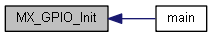
\includegraphics[width=231pt]{gpio_8h_ac724e431d2af879252de35615be2bdea_icgraph}
\end{center}
\end{figure}

\hypertarget{i2c_8h}{}\section{Inc/i2c.h File Reference}
\label{i2c_8h}\index{Inc/i2c.\+h@{Inc/i2c.\+h}}
{\ttfamily \#include \char`\"{}stm32f4xx\+\_\+hal.\+h\char`\"{}}\newline
{\ttfamily \#include \char`\"{}main.\+h\char`\"{}}\newline
Include dependency graph for i2c.\+h\+:\nopagebreak
\begin{figure}[H]
\begin{center}
\leavevmode
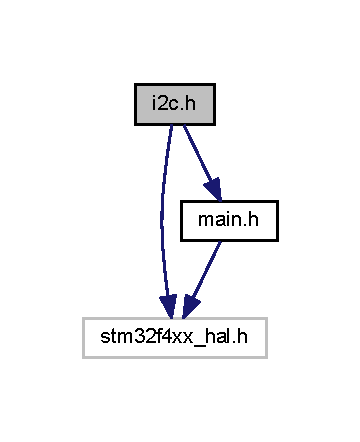
\includegraphics[width=173pt]{i2c_8h__incl}
\end{center}
\end{figure}
This graph shows which files directly or indirectly include this file\+:\nopagebreak
\begin{figure}[H]
\begin{center}
\leavevmode
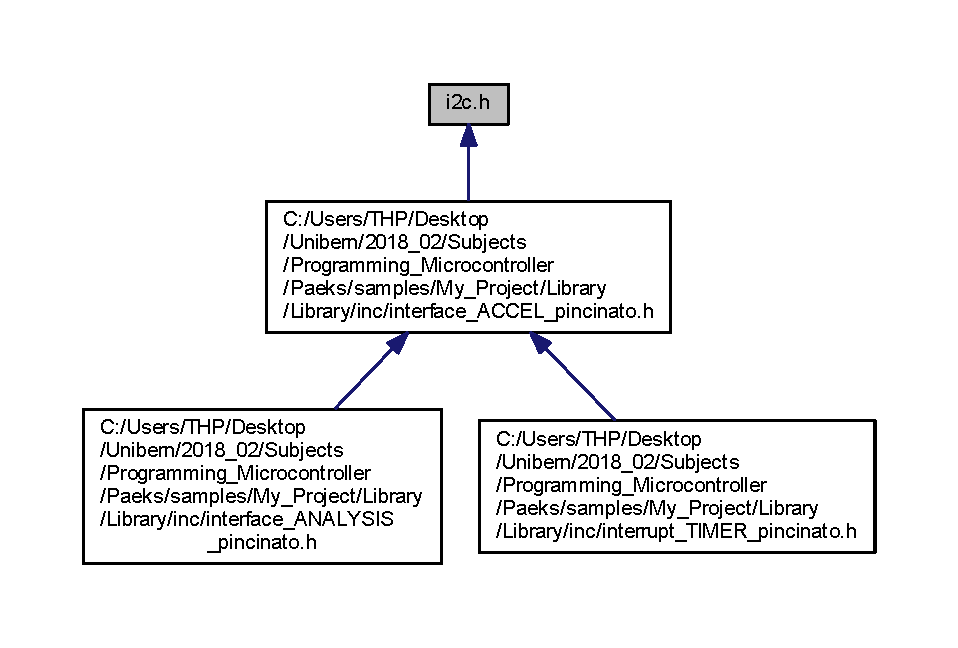
\includegraphics[width=350pt]{i2c_8h__dep__incl}
\end{center}
\end{figure}
\subsection*{Functions}
\begin{DoxyCompactItemize}
\item 
void \mbox{\hyperlink{i2c_8h_a47642651029b93e3f9c9edad46bd27b4}{\+\_\+\+Error\+\_\+\+Handler}} (char $\ast$, int)
\begin{DoxyCompactList}\small\item\em This function is executed in case of error occurrence. \end{DoxyCompactList}\item 
void \mbox{\hyperlink{i2c_8h_ada6e763cfa4108a8d24cd27b75f2f489}{M\+X\+\_\+\+I2\+C1\+\_\+\+Init}} (void)
\end{DoxyCompactItemize}
\subsection*{Variables}
\begin{DoxyCompactItemize}
\item 
I2\+C\+\_\+\+Handle\+Type\+Def \mbox{\hyperlink{i2c_8h_af7b2c26e44dadaaa798a5c3d82914ba7}{hi2c1}}
\end{DoxyCompactItemize}


\subsection{Function Documentation}
\mbox{\Hypertarget{i2c_8h_a47642651029b93e3f9c9edad46bd27b4}\label{i2c_8h_a47642651029b93e3f9c9edad46bd27b4}} 
\index{i2c.\+h@{i2c.\+h}!\+\_\+\+Error\+\_\+\+Handler@{\+\_\+\+Error\+\_\+\+Handler}}
\index{\+\_\+\+Error\+\_\+\+Handler@{\+\_\+\+Error\+\_\+\+Handler}!i2c.\+h@{i2c.\+h}}
\subsubsection{\texorpdfstring{\+\_\+\+Error\+\_\+\+Handler()}{\_Error\_Handler()}}
{\footnotesize\ttfamily void \+\_\+\+Error\+\_\+\+Handler (\begin{DoxyParamCaption}\item[{char $\ast$}]{file,  }\item[{int}]{line }\end{DoxyParamCaption})}



This function is executed in case of error occurrence. 


\begin{DoxyParams}{Parameters}
{\em file} & The file name as string. \\
\hline
{\em line} & The line in file as a number. \\
\hline
\end{DoxyParams}

\begin{DoxyRetVals}{Return values}
{\em None} & \\
\hline
\end{DoxyRetVals}


Definition at line 430 of file main.\+c.

\mbox{\Hypertarget{i2c_8h_ada6e763cfa4108a8d24cd27b75f2f489}\label{i2c_8h_ada6e763cfa4108a8d24cd27b75f2f489}} 
\index{i2c.\+h@{i2c.\+h}!M\+X\+\_\+\+I2\+C1\+\_\+\+Init@{M\+X\+\_\+\+I2\+C1\+\_\+\+Init}}
\index{M\+X\+\_\+\+I2\+C1\+\_\+\+Init@{M\+X\+\_\+\+I2\+C1\+\_\+\+Init}!i2c.\+h@{i2c.\+h}}
\subsubsection{\texorpdfstring{M\+X\+\_\+\+I2\+C1\+\_\+\+Init()}{MX\_I2C1\_Init()}}
{\footnotesize\ttfamily void M\+X\+\_\+\+I2\+C1\+\_\+\+Init (\begin{DoxyParamCaption}\item[{void}]{ }\end{DoxyParamCaption})}



Definition at line 62 of file i2c.\+c.

Here is the call graph for this function\+:\nopagebreak
\begin{figure}[H]
\begin{center}
\leavevmode
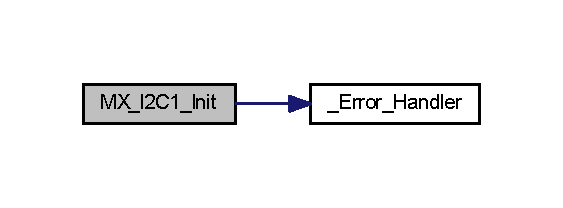
\includegraphics[width=270pt]{i2c_8h_ada6e763cfa4108a8d24cd27b75f2f489_cgraph}
\end{center}
\end{figure}
Here is the caller graph for this function\+:\nopagebreak
\begin{figure}[H]
\begin{center}
\leavevmode
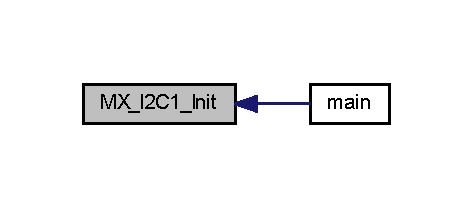
\includegraphics[width=227pt]{i2c_8h_ada6e763cfa4108a8d24cd27b75f2f489_icgraph}
\end{center}
\end{figure}


\subsection{Variable Documentation}
\mbox{\Hypertarget{i2c_8h_af7b2c26e44dadaaa798a5c3d82914ba7}\label{i2c_8h_af7b2c26e44dadaaa798a5c3d82914ba7}} 
\index{i2c.\+h@{i2c.\+h}!hi2c1@{hi2c1}}
\index{hi2c1@{hi2c1}!i2c.\+h@{i2c.\+h}}
\subsubsection{\texorpdfstring{hi2c1}{hi2c1}}
{\footnotesize\ttfamily I2\+C\+\_\+\+Handle\+Type\+Def hi2c1}

File Name \+: \mbox{\hyperlink{i2c_8h}{I2\+C.\+h}} Description \+: This file provides code for the configuration of the I2C instances.

This notice applies to any and all portions of this file that are not between comment pairs U\+S\+ER C\+O\+DE B\+E\+G\+IN and U\+S\+ER C\+O\+DE E\+ND. Other portions of this file, whether inserted by the user or by software development tools are owned by their respective copyright owners.

Copyright (c) 2018 S\+T\+Microelectronics International N.\+V. All rights reserved.

Redistribution and use in source and binary forms, with or without modification, are permitted, provided that the following conditions are met\+:


\begin{DoxyEnumerate}
\item Redistribution of source code must retain the above copyright notice, this list of conditions and the following disclaimer.
\item Redistributions in binary form must reproduce the above copyright notice, this list of conditions and the following disclaimer in the documentation and/or other materials provided with the distribution.
\item Neither the name of S\+T\+Microelectronics nor the names of other contributors to this software may be used to endorse or promote products derived from this software without specific written permission.
\item This software, including modifications and/or derivative works of this software, must execute solely and exclusively on microcontroller or microprocessor devices manufactured by or for S\+T\+Microelectronics.
\item Redistribution and use of this software other than as permitted under this license is void and will automatically terminate your rights under this license.
\end{DoxyEnumerate}

T\+H\+IS S\+O\+F\+T\+W\+A\+RE IS P\+R\+O\+V\+I\+D\+ED BY S\+T\+M\+I\+C\+R\+O\+E\+L\+E\+C\+T\+R\+O\+N\+I\+CS A\+ND C\+O\+N\+T\+R\+I\+B\+U\+T\+O\+RS \char`\"{}\+A\+S I\+S\char`\"{} A\+ND A\+NY E\+X\+P\+R\+E\+SS, I\+M\+P\+L\+I\+ED OR S\+T\+A\+T\+U\+T\+O\+RY W\+A\+R\+R\+A\+N\+T\+I\+ES, I\+N\+C\+L\+U\+D\+I\+NG, B\+UT N\+OT L\+I\+M\+I\+T\+ED TO, T\+HE I\+M\+P\+L\+I\+ED W\+A\+R\+R\+A\+N\+T\+I\+ES OF M\+E\+R\+C\+H\+A\+N\+T\+A\+B\+I\+L\+I\+TY, F\+I\+T\+N\+E\+SS F\+OR A P\+A\+R\+T\+I\+C\+U\+L\+AR P\+U\+R\+P\+O\+SE A\+ND N\+O\+N-\/\+I\+N\+F\+R\+I\+N\+G\+E\+M\+E\+NT OF T\+H\+I\+RD P\+A\+R\+TY I\+N\+T\+E\+L\+L\+E\+C\+T\+U\+AL P\+R\+O\+P\+E\+R\+TY R\+I\+G\+H\+TS A\+RE D\+I\+S\+C\+L\+A\+I\+M\+ED TO T\+HE F\+U\+L\+L\+E\+ST E\+X\+T\+E\+NT P\+E\+R\+M\+I\+T\+T\+ED BY L\+AW. IN NO E\+V\+E\+NT S\+H\+A\+LL S\+T\+M\+I\+C\+R\+O\+E\+L\+E\+C\+T\+R\+O\+N\+I\+CS OR C\+O\+N\+T\+R\+I\+B\+U\+T\+O\+RS BE L\+I\+A\+B\+LE F\+OR A\+NY D\+I\+R\+E\+CT, I\+N\+D\+I\+R\+E\+CT, I\+N\+C\+I\+D\+E\+N\+T\+AL, S\+P\+E\+C\+I\+AL, E\+X\+E\+M\+P\+L\+A\+RY, OR C\+O\+N\+S\+E\+Q\+U\+E\+N\+T\+I\+AL D\+A\+M\+A\+G\+ES (I\+N\+C\+L\+U\+D\+I\+NG, B\+UT N\+OT L\+I\+M\+I\+T\+ED TO, P\+R\+O\+C\+U\+R\+E\+M\+E\+NT OF S\+U\+B\+S\+T\+I\+T\+U\+TE G\+O\+O\+DS OR S\+E\+R\+V\+I\+C\+ES; L\+O\+SS OF U\+SE, D\+A\+TA, OR P\+R\+O\+F\+I\+TS; OR B\+U\+S\+I\+N\+E\+SS I\+N\+T\+E\+R\+R\+U\+P\+T\+I\+ON) H\+O\+W\+E\+V\+ER C\+A\+U\+S\+ED A\+ND ON A\+NY T\+H\+E\+O\+RY OF L\+I\+A\+B\+I\+L\+I\+TY, W\+H\+E\+T\+H\+ER IN C\+O\+N\+T\+R\+A\+CT, S\+T\+R\+I\+CT L\+I\+A\+B\+I\+L\+I\+TY, OR T\+O\+RT (I\+N\+C\+L\+U\+D\+I\+NG N\+E\+G\+L\+I\+G\+E\+N\+CE OR O\+T\+H\+E\+R\+W\+I\+SE) A\+R\+I\+S\+I\+NG IN A\+NY W\+AY O\+UT OF T\+HE U\+SE OF T\+H\+IS S\+O\+F\+T\+W\+A\+RE, E\+V\+EN IF A\+D\+V\+I\+S\+ED OF T\+HE P\+O\+S\+S\+I\+B\+I\+L\+I\+TY OF S\+U\+CH D\+A\+M\+A\+GE.

File Name \+: \mbox{\hyperlink{i2c_8c}{I2\+C.\+c}} Description \+: This file provides code for the configuration of the I2C instances.

This notice applies to any and all portions of this file that are not between comment pairs U\+S\+ER C\+O\+DE B\+E\+G\+IN and U\+S\+ER C\+O\+DE E\+ND. Other portions of this file, whether inserted by the user or by software development tools are owned by their respective copyright owners.

Copyright (c) 2018 S\+T\+Microelectronics International N.\+V. All rights reserved.

Redistribution and use in source and binary forms, with or without modification, are permitted, provided that the following conditions are met\+:


\begin{DoxyEnumerate}
\item Redistribution of source code must retain the above copyright notice, this list of conditions and the following disclaimer.
\item Redistributions in binary form must reproduce the above copyright notice, this list of conditions and the following disclaimer in the documentation and/or other materials provided with the distribution.
\item Neither the name of S\+T\+Microelectronics nor the names of other contributors to this software may be used to endorse or promote products derived from this software without specific written permission.
\item This software, including modifications and/or derivative works of this software, must execute solely and exclusively on microcontroller or microprocessor devices manufactured by or for S\+T\+Microelectronics.
\item Redistribution and use of this software other than as permitted under this license is void and will automatically terminate your rights under this license.
\end{DoxyEnumerate}

T\+H\+IS S\+O\+F\+T\+W\+A\+RE IS P\+R\+O\+V\+I\+D\+ED BY S\+T\+M\+I\+C\+R\+O\+E\+L\+E\+C\+T\+R\+O\+N\+I\+CS A\+ND C\+O\+N\+T\+R\+I\+B\+U\+T\+O\+RS \char`\"{}\+A\+S I\+S\char`\"{} A\+ND A\+NY E\+X\+P\+R\+E\+SS, I\+M\+P\+L\+I\+ED OR S\+T\+A\+T\+U\+T\+O\+RY W\+A\+R\+R\+A\+N\+T\+I\+ES, I\+N\+C\+L\+U\+D\+I\+NG, B\+UT N\+OT L\+I\+M\+I\+T\+ED TO, T\+HE I\+M\+P\+L\+I\+ED W\+A\+R\+R\+A\+N\+T\+I\+ES OF M\+E\+R\+C\+H\+A\+N\+T\+A\+B\+I\+L\+I\+TY, F\+I\+T\+N\+E\+SS F\+OR A P\+A\+R\+T\+I\+C\+U\+L\+AR P\+U\+R\+P\+O\+SE A\+ND N\+O\+N-\/\+I\+N\+F\+R\+I\+N\+G\+E\+M\+E\+NT OF T\+H\+I\+RD P\+A\+R\+TY I\+N\+T\+E\+L\+L\+E\+C\+T\+U\+AL P\+R\+O\+P\+E\+R\+TY R\+I\+G\+H\+TS A\+RE D\+I\+S\+C\+L\+A\+I\+M\+ED TO T\+HE F\+U\+L\+L\+E\+ST E\+X\+T\+E\+NT P\+E\+R\+M\+I\+T\+T\+ED BY L\+AW. IN NO E\+V\+E\+NT S\+H\+A\+LL S\+T\+M\+I\+C\+R\+O\+E\+L\+E\+C\+T\+R\+O\+N\+I\+CS OR C\+O\+N\+T\+R\+I\+B\+U\+T\+O\+RS BE L\+I\+A\+B\+LE F\+OR A\+NY D\+I\+R\+E\+CT, I\+N\+D\+I\+R\+E\+CT, I\+N\+C\+I\+D\+E\+N\+T\+AL, S\+P\+E\+C\+I\+AL, E\+X\+E\+M\+P\+L\+A\+RY, OR C\+O\+N\+S\+E\+Q\+U\+E\+N\+T\+I\+AL D\+A\+M\+A\+G\+ES (I\+N\+C\+L\+U\+D\+I\+NG, B\+UT N\+OT L\+I\+M\+I\+T\+ED TO, P\+R\+O\+C\+U\+R\+E\+M\+E\+NT OF S\+U\+B\+S\+T\+I\+T\+U\+TE G\+O\+O\+DS OR S\+E\+R\+V\+I\+C\+ES; L\+O\+SS OF U\+SE, D\+A\+TA, OR P\+R\+O\+F\+I\+TS; OR B\+U\+S\+I\+N\+E\+SS I\+N\+T\+E\+R\+R\+U\+P\+T\+I\+ON) H\+O\+W\+E\+V\+ER C\+A\+U\+S\+ED A\+ND ON A\+NY T\+H\+E\+O\+RY OF L\+I\+A\+B\+I\+L\+I\+TY, W\+H\+E\+T\+H\+ER IN C\+O\+N\+T\+R\+A\+CT, S\+T\+R\+I\+CT L\+I\+A\+B\+I\+L\+I\+TY, OR T\+O\+RT (I\+N\+C\+L\+U\+D\+I\+NG N\+E\+G\+L\+I\+G\+E\+N\+CE OR O\+T\+H\+E\+R\+W\+I\+SE) A\+R\+I\+S\+I\+NG IN A\+NY W\+AY O\+UT OF T\+HE U\+SE OF T\+H\+IS S\+O\+F\+T\+W\+A\+RE, E\+V\+EN IF A\+D\+V\+I\+S\+ED OF T\+HE P\+O\+S\+S\+I\+B\+I\+L\+I\+TY OF S\+U\+CH D\+A\+M\+A\+GE. 

Definition at line 59 of file i2c.\+c.


\hypertarget{main_8h}{}\section{main.\+h File Reference}
\label{main_8h}\index{main.\+h@{main.\+h}}


\+: Header for main.\+c file. This file contains the common defines of the application.  


{\ttfamily \#include \char`\"{}stm32f4xx\+\_\+hal.\+h\char`\"{}}\newline
Include dependency graph for main.\+h\+:\nopagebreak
\begin{figure}[H]
\begin{center}
\leavevmode
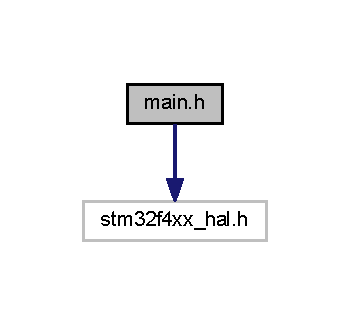
\includegraphics[width=168pt]{main_8h__incl}
\end{center}
\end{figure}
This graph shows which files directly or indirectly include this file\+:\nopagebreak
\begin{figure}[H]
\begin{center}
\leavevmode
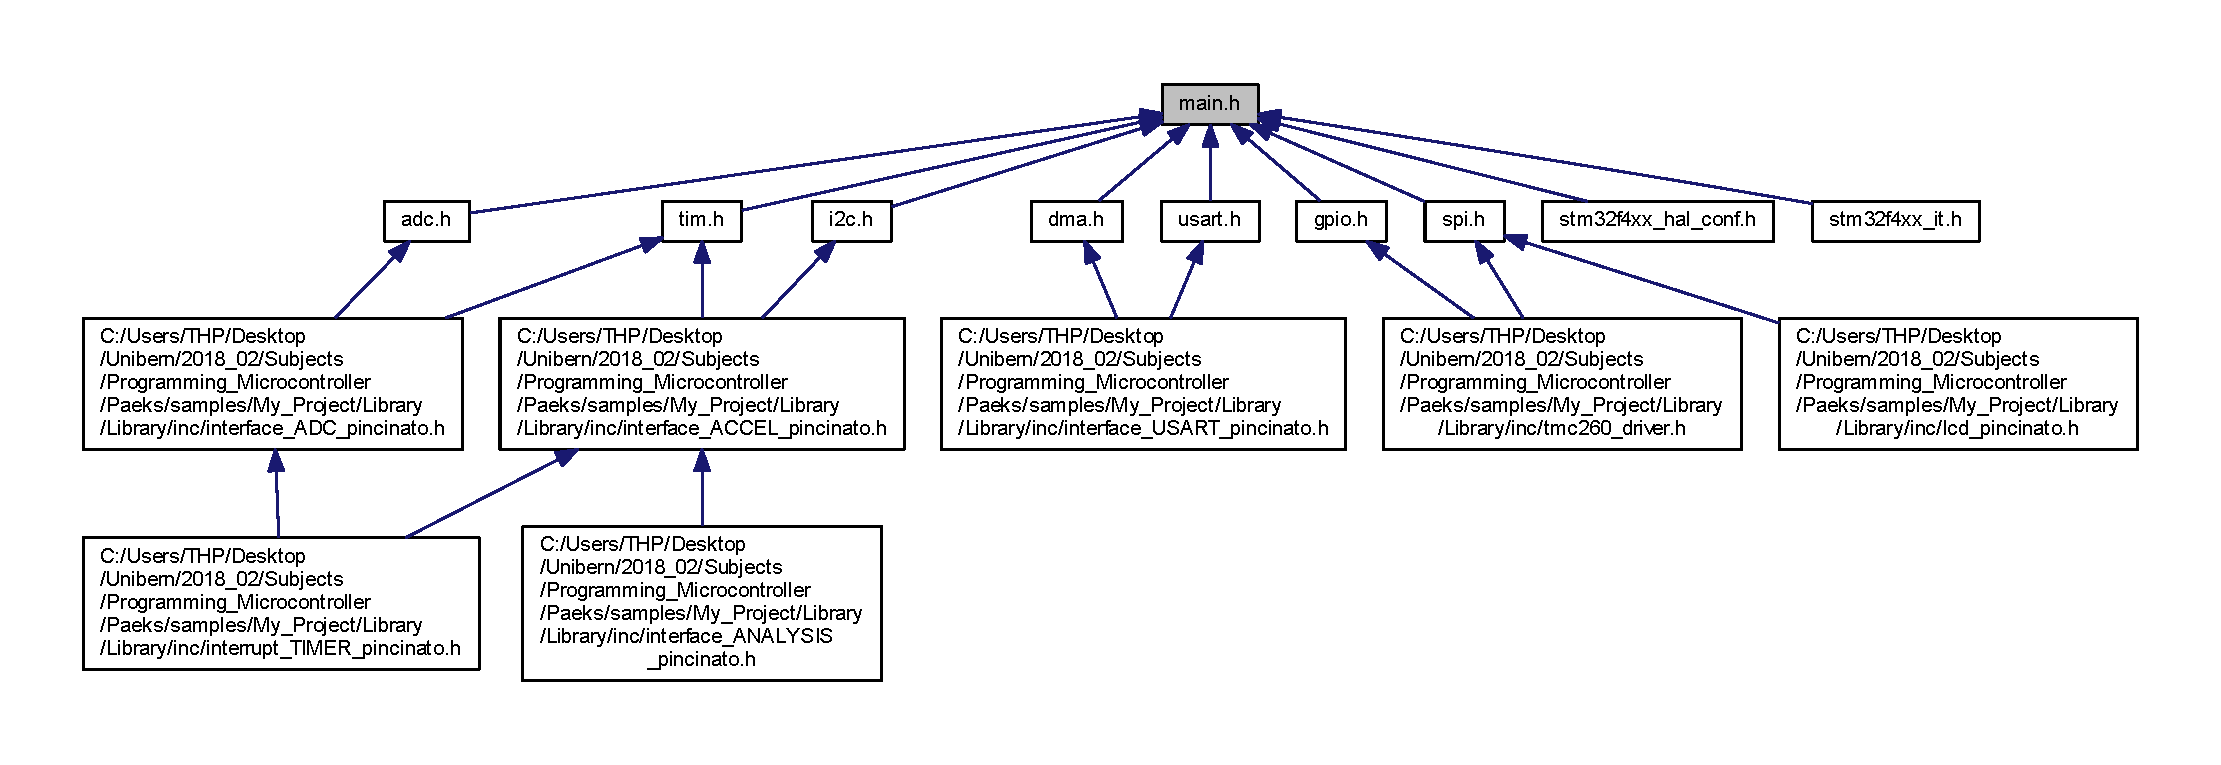
\includegraphics[width=350pt]{main_8h__dep__incl}
\end{center}
\end{figure}
\subsection*{Macros}
\begin{DoxyCompactItemize}
\item 
\#define \mbox{\hyperlink{main_8h_ae2f744343ecfa5e1667ef68ab5a4e73a}{S\+W\+I\+T\+C\+H\+\_\+\+R\+I\+G\+H\+T\+\_\+\+Pin}}~G\+P\+I\+O\+\_\+\+P\+I\+N\+\_\+0
\item 
\#define \mbox{\hyperlink{main_8h_ab74048af6f7e1b0462ed815ee026e159}{S\+W\+I\+T\+C\+H\+\_\+\+R\+I\+G\+H\+T\+\_\+\+G\+P\+I\+O\+\_\+\+Port}}~G\+P\+I\+OC
\item 
\#define \mbox{\hyperlink{main_8h_abb659625724ea98453a5e193d33c66fc}{S\+W\+I\+T\+C\+H\+\_\+\+L\+E\+F\+T\+\_\+\+Pin}}~G\+P\+I\+O\+\_\+\+P\+I\+N\+\_\+1
\item 
\#define \mbox{\hyperlink{main_8h_a3d154aa9ca4d5562d1836fff6c6aa581}{S\+W\+I\+T\+C\+H\+\_\+\+L\+E\+F\+T\+\_\+\+G\+P\+I\+O\+\_\+\+Port}}~G\+P\+I\+OC
\item 
\#define \mbox{\hyperlink{main_8h_a29da69d4d05cd560d42cdfe217a8ed68}{L\+O\+\_\+\+\_\+\+Input\+\_\+\+Pin}}~G\+P\+I\+O\+\_\+\+P\+I\+N\+\_\+2
\item 
\#define \mbox{\hyperlink{main_8h_a0ff972c5cbe09bcbffb923203f0d14d3}{L\+O\+\_\+\+\_\+\+Input\+\_\+\+G\+P\+I\+O\+\_\+\+Port}}~G\+P\+I\+OC
\item 
\#define \mbox{\hyperlink{main_8h_a8571429cac36c31d021425f2bf2e8449}{L\+O\+\_\+\+\_\+\+Input\+C3\+\_\+\+Pin}}~G\+P\+I\+O\+\_\+\+P\+I\+N\+\_\+3
\item 
\#define \mbox{\hyperlink{main_8h_a363e08d2e80a6824d9cb67286daed677}{L\+O\+\_\+\+\_\+\+Input\+C3\+\_\+\+G\+P\+I\+O\+\_\+\+Port}}~G\+P\+I\+OC
\item 
\#define \mbox{\hyperlink{main_8h_a0b2b1cef7aa617342c6fa3ccbcb4ef67}{P\+O\+T\+\_\+2\+\_\+\+Pin}}~G\+P\+I\+O\+\_\+\+P\+I\+N\+\_\+1
\item 
\#define \mbox{\hyperlink{main_8h_a2912f1291506a63956d2a5b4197ae7cc}{P\+O\+T\+\_\+2\+\_\+\+G\+P\+I\+O\+\_\+\+Port}}~G\+P\+I\+OA
\item 
\#define \mbox{\hyperlink{main_8h_a789955dda0fefefaa54a97d31408ae74}{S\+W\+I\+T\+C\+H\+\_\+\+U\+P\+\_\+\+Pin}}~G\+P\+I\+O\+\_\+\+P\+I\+N\+\_\+4
\item 
\#define \mbox{\hyperlink{main_8h_a1a4a5f94c629ca88c411a7964d648023}{S\+W\+I\+T\+C\+H\+\_\+\+U\+P\+\_\+\+G\+P\+I\+O\+\_\+\+Port}}~G\+P\+I\+OA
\item 
\#define \mbox{\hyperlink{main_8h_ac1e43ce9089f8f473272aa03c671dd0b}{L\+C\+D\+\_\+\+S\+C\+K\+\_\+\+Pin}}~G\+P\+I\+O\+\_\+\+P\+I\+N\+\_\+5
\item 
\#define \mbox{\hyperlink{main_8h_a9882dd3b88368c7e4c108ea5b8305645}{L\+C\+D\+\_\+\+S\+C\+K\+\_\+\+G\+P\+I\+O\+\_\+\+Port}}~G\+P\+I\+OA
\item 
\#define \mbox{\hyperlink{main_8h_a9a82735e4c6ff7e421c4de32e99975dc}{L\+C\+D\+\_\+\+R\+E\+S\+E\+T\+\_\+\+Pin}}~G\+P\+I\+O\+\_\+\+P\+I\+N\+\_\+6
\item 
\#define \mbox{\hyperlink{main_8h_a9ed56de0ffbd06c94af651b685fe5783}{L\+C\+D\+\_\+\+R\+E\+S\+E\+T\+\_\+\+G\+P\+I\+O\+\_\+\+Port}}~G\+P\+I\+OA
\item 
\#define \mbox{\hyperlink{main_8h_a319ce1edd2d6fbb710105afe2bcd9259}{L\+C\+D\+\_\+\+M\+O\+S\+I\+\_\+\+Pin}}~G\+P\+I\+O\+\_\+\+P\+I\+N\+\_\+7
\item 
\#define \mbox{\hyperlink{main_8h_abdf42c0e7b8b4158b1e0bb6509dfde3c}{L\+C\+D\+\_\+\+M\+O\+S\+I\+\_\+\+G\+P\+I\+O\+\_\+\+Port}}~G\+P\+I\+OA
\item 
\#define \mbox{\hyperlink{main_8h_ad039ac1b284751bbe9ed07cf7ee40301}{S\+W\+I\+T\+C\+H\+\_\+\+D\+O\+W\+N\+\_\+\+Pin}}~G\+P\+I\+O\+\_\+\+P\+I\+N\+\_\+0
\item 
\#define \mbox{\hyperlink{main_8h_ae76acb2eaac2f7cdc9ec9aab2d4885b2}{S\+W\+I\+T\+C\+H\+\_\+\+D\+O\+W\+N\+\_\+\+G\+P\+I\+O\+\_\+\+Port}}~G\+P\+I\+OB
\item 
\#define \mbox{\hyperlink{main_8h_a86e74b3df6ffff3813b38feec50ed957}{A\+D\+C\+\_\+\+Input\+\_\+\+Pin}}~G\+P\+I\+O\+\_\+\+P\+I\+N\+\_\+1
\item 
\#define \mbox{\hyperlink{main_8h_aa7f50bb0def206315edc43e20c5e634a}{A\+D\+C\+\_\+\+Input\+\_\+\+G\+P\+I\+O\+\_\+\+Port}}~G\+P\+I\+OB
\item 
\#define \mbox{\hyperlink{main_8h_a312b955bd1c301297c912818f4dbc858}{Card\+Detected\+\_\+\+Pin}}~G\+P\+I\+O\+\_\+\+P\+I\+N\+\_\+12
\item 
\#define \mbox{\hyperlink{main_8h_acabcfe4e7ed511c5a5ca9dd2a56c4a71}{Card\+Detected\+\_\+\+G\+P\+I\+O\+\_\+\+Port}}~G\+P\+I\+OB
\item 
\#define \mbox{\hyperlink{main_8h_a1cefd73847ad433f624034a5e3b03f79}{S\+P\+I2\+\_\+\+C\+S\+\_\+\+Pin}}~G\+P\+I\+O\+\_\+\+P\+I\+N\+\_\+6
\item 
\#define \mbox{\hyperlink{main_8h_ad2875a38a73431ff5df574415e4517f0}{S\+P\+I2\+\_\+\+C\+S\+\_\+\+G\+P\+I\+O\+\_\+\+Port}}~G\+P\+I\+OC
\item 
\#define \mbox{\hyperlink{main_8h_ab7e9ff1b5342520b116cab82117f4a73}{Led\+Green\+\_\+\+Pin}}~G\+P\+I\+O\+\_\+\+P\+I\+N\+\_\+7
\item 
\#define \mbox{\hyperlink{main_8h_a473e03f2e0aa7a8dc739e6302de5ca7a}{Led\+Green\+\_\+\+G\+P\+I\+O\+\_\+\+Port}}~G\+P\+I\+OC
\item 
\#define \mbox{\hyperlink{main_8h_ab72b3b1a64f4dea34c70abca0fe939f2}{L\+C\+D\+\_\+\+A0\+\_\+\+Pin}}~G\+P\+I\+O\+\_\+\+P\+I\+N\+\_\+8
\item 
\#define \mbox{\hyperlink{main_8h_a0edb1511065e67fd6f624622cd184daa}{L\+C\+D\+\_\+\+A0\+\_\+\+G\+P\+I\+O\+\_\+\+Port}}~G\+P\+I\+OA
\item 
\#define \mbox{\hyperlink{main_8h_a7bc602a9f1c466218c53e3f48fe7ad40}{Led\+Blue\+\_\+\+Pin}}~G\+P\+I\+O\+\_\+\+P\+I\+N\+\_\+9
\item 
\#define \mbox{\hyperlink{main_8h_a79349bfd6f7b0ac790548ff60198a511}{Led\+Blue\+\_\+\+G\+P\+I\+O\+\_\+\+Port}}~G\+P\+I\+OA
\item 
\#define \mbox{\hyperlink{main_8h_a15bcb1112410041b6d51e954d58d129b}{L\+E\+D\+\_\+\+R\+E\+D\+\_\+\+Pin}}~G\+P\+I\+O\+\_\+\+P\+I\+N\+\_\+4
\item 
\#define \mbox{\hyperlink{main_8h_a8a4e80fa39d14daa8305680135261903}{L\+E\+D\+\_\+\+R\+E\+D\+\_\+\+G\+P\+I\+O\+\_\+\+Port}}~G\+P\+I\+OB
\item 
\#define \mbox{\hyperlink{main_8h_a5720ca9abbb36f2cf19e7813fafd37e6}{S\+W\+I\+T\+C\+H\+\_\+\+C\+E\+N\+T\+E\+R\+\_\+\+Pin}}~G\+P\+I\+O\+\_\+\+P\+I\+N\+\_\+5
\item 
\#define \mbox{\hyperlink{main_8h_a30bab443bc005c6d8bda0586b42c0e4b}{S\+W\+I\+T\+C\+H\+\_\+\+C\+E\+N\+T\+E\+R\+\_\+\+G\+P\+I\+O\+\_\+\+Port}}~G\+P\+I\+OB
\item 
\#define \mbox{\hyperlink{main_8h_a8ce42d96513be68fd9bf20a303c43e8b}{L\+C\+D\+\_\+\+C\+S\+\_\+\+N\+\_\+\+Pin}}~G\+P\+I\+O\+\_\+\+P\+I\+N\+\_\+6
\item 
\#define \mbox{\hyperlink{main_8h_ae51bed3af627a82fc2aa22afe40de08c}{L\+C\+D\+\_\+\+C\+S\+\_\+\+N\+\_\+\+G\+P\+I\+O\+\_\+\+Port}}~G\+P\+I\+OB
\item 
\#define \mbox{\hyperlink{main_8h_af39838801cb65b958ec9a539cb64898d}{F\+A\+T\+F\+S\+\_\+\+U\+S\+E\+\_\+\+S\+D\+IO}}~0
\begin{DoxyCompactList}\small\item\em Uncomment the line below to expanse the \char`\"{}assert\+\_\+param\char`\"{} macro in the H\+AL drivers code. \end{DoxyCompactList}\item 
\#define \mbox{\hyperlink{main_8h_a05a8b0232e4368dd8a360c854a0a684e}{F\+A\+T\+F\+S\+\_\+\+S\+PI}}~S\+P\+I2
\item 
\#define \mbox{\hyperlink{main_8h_aad8a58124b9ad8800e6e11fa32c2d00a}{F\+A\+T\+F\+S\+\_\+\+S\+P\+I\+\_\+\+P\+I\+N\+S\+P\+A\+CK}}~T\+M\+\_\+\+S\+P\+I\+\_\+\+Pins\+Pack\+\_\+2
\item 
\#define \mbox{\hyperlink{main_8h_a49ec20d7b95553c4002675dd2147579b}{F\+A\+T\+\_\+\+S\+D\+\_\+\+S\+PI}}~\mbox{\hyperlink{spi_8h_ab9da65f935e805137e2eb4e18c5ab224}{hspi2}}
\item 
\#define \mbox{\hyperlink{main_8h_a5593abbf196bdbd410b0939ef878b9d1}{Error\+\_\+\+Handler}}()~\mbox{\hyperlink{usart_8h_a47642651029b93e3f9c9edad46bd27b4}{\+\_\+\+Error\+\_\+\+Handler}}(\+\_\+\+\_\+\+F\+I\+L\+E\+\_\+\+\_\+, \+\_\+\+\_\+\+L\+I\+N\+E\+\_\+\+\_\+)
\end{DoxyCompactItemize}
\subsection*{Functions}
\begin{DoxyCompactItemize}
\item 
void \mbox{\hyperlink{main_8h_a47642651029b93e3f9c9edad46bd27b4}{\+\_\+\+Error\+\_\+\+Handler}} (char $\ast$, int)
\end{DoxyCompactItemize}


\subsection{Detailed Description}
\+: Header for main.\+c file. This file contains the common defines of the application. 

This notice applies to any and all portions of this file that are not between comment pairs U\+S\+ER C\+O\+DE B\+E\+G\+IN and U\+S\+ER C\+O\+DE E\+ND. Other portions of this file, whether inserted by the user or by software development tools are owned by their respective copyright owners.

Copyright (c) 2018 S\+T\+Microelectronics International N.\+V. All rights reserved.

Redistribution and use in source and binary forms, with or without modification, are permitted, provided that the following conditions are met\+:


\begin{DoxyEnumerate}
\item Redistribution of source code must retain the above copyright notice, this list of conditions and the following disclaimer.
\item Redistributions in binary form must reproduce the above copyright notice, this list of conditions and the following disclaimer in the documentation and/or other materials provided with the distribution.
\item Neither the name of S\+T\+Microelectronics nor the names of other contributors to this software may be used to endorse or promote products derived from this software without specific written permission.
\item This software, including modifications and/or derivative works of this software, must execute solely and exclusively on microcontroller or microprocessor devices manufactured by or for S\+T\+Microelectronics.
\item Redistribution and use of this software other than as permitted under this license is void and will automatically terminate your rights under this license.
\end{DoxyEnumerate}

T\+H\+IS S\+O\+F\+T\+W\+A\+RE IS P\+R\+O\+V\+I\+D\+ED BY S\+T\+M\+I\+C\+R\+O\+E\+L\+E\+C\+T\+R\+O\+N\+I\+CS A\+ND C\+O\+N\+T\+R\+I\+B\+U\+T\+O\+RS \char`\"{}\+A\+S I\+S\char`\"{} A\+ND A\+NY E\+X\+P\+R\+E\+SS, I\+M\+P\+L\+I\+ED OR S\+T\+A\+T\+U\+T\+O\+RY W\+A\+R\+R\+A\+N\+T\+I\+ES, I\+N\+C\+L\+U\+D\+I\+NG, B\+UT N\+OT L\+I\+M\+I\+T\+ED TO, T\+HE I\+M\+P\+L\+I\+ED W\+A\+R\+R\+A\+N\+T\+I\+ES OF M\+E\+R\+C\+H\+A\+N\+T\+A\+B\+I\+L\+I\+TY, F\+I\+T\+N\+E\+SS F\+OR A P\+A\+R\+T\+I\+C\+U\+L\+AR P\+U\+R\+P\+O\+SE A\+ND N\+O\+N-\/\+I\+N\+F\+R\+I\+N\+G\+E\+M\+E\+NT OF T\+H\+I\+RD P\+A\+R\+TY I\+N\+T\+E\+L\+L\+E\+C\+T\+U\+AL P\+R\+O\+P\+E\+R\+TY R\+I\+G\+H\+TS A\+RE D\+I\+S\+C\+L\+A\+I\+M\+ED TO T\+HE F\+U\+L\+L\+E\+ST E\+X\+T\+E\+NT P\+E\+R\+M\+I\+T\+T\+ED BY L\+AW. IN NO E\+V\+E\+NT S\+H\+A\+LL S\+T\+M\+I\+C\+R\+O\+E\+L\+E\+C\+T\+R\+O\+N\+I\+CS OR C\+O\+N\+T\+R\+I\+B\+U\+T\+O\+RS BE L\+I\+A\+B\+LE F\+OR A\+NY D\+I\+R\+E\+CT, I\+N\+D\+I\+R\+E\+CT, I\+N\+C\+I\+D\+E\+N\+T\+AL, S\+P\+E\+C\+I\+AL, E\+X\+E\+M\+P\+L\+A\+RY, OR C\+O\+N\+S\+E\+Q\+U\+E\+N\+T\+I\+AL D\+A\+M\+A\+G\+ES (I\+N\+C\+L\+U\+D\+I\+NG, B\+UT N\+OT L\+I\+M\+I\+T\+ED TO, P\+R\+O\+C\+U\+R\+E\+M\+E\+NT OF S\+U\+B\+S\+T\+I\+T\+U\+TE G\+O\+O\+DS OR S\+E\+R\+V\+I\+C\+ES; L\+O\+SS OF U\+SE, D\+A\+TA, OR P\+R\+O\+F\+I\+TS; OR B\+U\+S\+I\+N\+E\+SS I\+N\+T\+E\+R\+R\+U\+P\+T\+I\+ON) H\+O\+W\+E\+V\+ER C\+A\+U\+S\+ED A\+ND ON A\+NY T\+H\+E\+O\+RY OF L\+I\+A\+B\+I\+L\+I\+TY, W\+H\+E\+T\+H\+ER IN C\+O\+N\+T\+R\+A\+CT, S\+T\+R\+I\+CT L\+I\+A\+B\+I\+L\+I\+TY, OR T\+O\+RT (I\+N\+C\+L\+U\+D\+I\+NG N\+E\+G\+L\+I\+G\+E\+N\+CE OR O\+T\+H\+E\+R\+W\+I\+SE) A\+R\+I\+S\+I\+NG IN A\+NY W\+AY O\+UT OF T\+HE U\+SE OF T\+H\+IS S\+O\+F\+T\+W\+A\+RE, E\+V\+EN IF A\+D\+V\+I\+S\+ED OF T\+HE P\+O\+S\+S\+I\+B\+I\+L\+I\+TY OF S\+U\+CH D\+A\+M\+A\+GE. 

\subsection{Macro Definition Documentation}
\mbox{\Hypertarget{main_8h_aa7f50bb0def206315edc43e20c5e634a}\label{main_8h_aa7f50bb0def206315edc43e20c5e634a}} 
\index{main.\+h@{main.\+h}!A\+D\+C\+\_\+\+Input\+\_\+\+G\+P\+I\+O\+\_\+\+Port@{A\+D\+C\+\_\+\+Input\+\_\+\+G\+P\+I\+O\+\_\+\+Port}}
\index{A\+D\+C\+\_\+\+Input\+\_\+\+G\+P\+I\+O\+\_\+\+Port@{A\+D\+C\+\_\+\+Input\+\_\+\+G\+P\+I\+O\+\_\+\+Port}!main.\+h@{main.\+h}}
\subsubsection{\texorpdfstring{A\+D\+C\+\_\+\+Input\+\_\+\+G\+P\+I\+O\+\_\+\+Port}{ADC\_Input\_GPIO\_Port}}
{\footnotesize\ttfamily \#define A\+D\+C\+\_\+\+Input\+\_\+\+G\+P\+I\+O\+\_\+\+Port~G\+P\+I\+OB}



Definition at line 84 of file main.\+h.

\mbox{\Hypertarget{main_8h_a86e74b3df6ffff3813b38feec50ed957}\label{main_8h_a86e74b3df6ffff3813b38feec50ed957}} 
\index{main.\+h@{main.\+h}!A\+D\+C\+\_\+\+Input\+\_\+\+Pin@{A\+D\+C\+\_\+\+Input\+\_\+\+Pin}}
\index{A\+D\+C\+\_\+\+Input\+\_\+\+Pin@{A\+D\+C\+\_\+\+Input\+\_\+\+Pin}!main.\+h@{main.\+h}}
\subsubsection{\texorpdfstring{A\+D\+C\+\_\+\+Input\+\_\+\+Pin}{ADC\_Input\_Pin}}
{\footnotesize\ttfamily \#define A\+D\+C\+\_\+\+Input\+\_\+\+Pin~G\+P\+I\+O\+\_\+\+P\+I\+N\+\_\+1}



Definition at line 83 of file main.\+h.

\mbox{\Hypertarget{main_8h_acabcfe4e7ed511c5a5ca9dd2a56c4a71}\label{main_8h_acabcfe4e7ed511c5a5ca9dd2a56c4a71}} 
\index{main.\+h@{main.\+h}!Card\+Detected\+\_\+\+G\+P\+I\+O\+\_\+\+Port@{Card\+Detected\+\_\+\+G\+P\+I\+O\+\_\+\+Port}}
\index{Card\+Detected\+\_\+\+G\+P\+I\+O\+\_\+\+Port@{Card\+Detected\+\_\+\+G\+P\+I\+O\+\_\+\+Port}!main.\+h@{main.\+h}}
\subsubsection{\texorpdfstring{Card\+Detected\+\_\+\+G\+P\+I\+O\+\_\+\+Port}{CardDetected\_GPIO\_Port}}
{\footnotesize\ttfamily \#define Card\+Detected\+\_\+\+G\+P\+I\+O\+\_\+\+Port~G\+P\+I\+OB}



Definition at line 86 of file main.\+h.

\mbox{\Hypertarget{main_8h_a312b955bd1c301297c912818f4dbc858}\label{main_8h_a312b955bd1c301297c912818f4dbc858}} 
\index{main.\+h@{main.\+h}!Card\+Detected\+\_\+\+Pin@{Card\+Detected\+\_\+\+Pin}}
\index{Card\+Detected\+\_\+\+Pin@{Card\+Detected\+\_\+\+Pin}!main.\+h@{main.\+h}}
\subsubsection{\texorpdfstring{Card\+Detected\+\_\+\+Pin}{CardDetected\_Pin}}
{\footnotesize\ttfamily \#define Card\+Detected\+\_\+\+Pin~G\+P\+I\+O\+\_\+\+P\+I\+N\+\_\+12}



Definition at line 85 of file main.\+h.

\mbox{\Hypertarget{main_8h_a5593abbf196bdbd410b0939ef878b9d1}\label{main_8h_a5593abbf196bdbd410b0939ef878b9d1}} 
\index{main.\+h@{main.\+h}!Error\+\_\+\+Handler@{Error\+\_\+\+Handler}}
\index{Error\+\_\+\+Handler@{Error\+\_\+\+Handler}!main.\+h@{main.\+h}}
\subsubsection{\texorpdfstring{Error\+\_\+\+Handler}{Error\_Handler}}
{\footnotesize\ttfamily \#define Error\+\_\+\+Handler(\begin{DoxyParamCaption}{ }\end{DoxyParamCaption})~\mbox{\hyperlink{usart_8h_a47642651029b93e3f9c9edad46bd27b4}{\+\_\+\+Error\+\_\+\+Handler}}(\+\_\+\+\_\+\+F\+I\+L\+E\+\_\+\+\_\+, \+\_\+\+\_\+\+L\+I\+N\+E\+\_\+\+\_\+)}



Definition at line 125 of file main.\+h.

\mbox{\Hypertarget{main_8h_a49ec20d7b95553c4002675dd2147579b}\label{main_8h_a49ec20d7b95553c4002675dd2147579b}} 
\index{main.\+h@{main.\+h}!F\+A\+T\+\_\+\+S\+D\+\_\+\+S\+PI@{F\+A\+T\+\_\+\+S\+D\+\_\+\+S\+PI}}
\index{F\+A\+T\+\_\+\+S\+D\+\_\+\+S\+PI@{F\+A\+T\+\_\+\+S\+D\+\_\+\+S\+PI}!main.\+h@{main.\+h}}
\subsubsection{\texorpdfstring{F\+A\+T\+\_\+\+S\+D\+\_\+\+S\+PI}{FAT\_SD\_SPI}}
{\footnotesize\ttfamily \#define F\+A\+T\+\_\+\+S\+D\+\_\+\+S\+PI~\mbox{\hyperlink{spi_8h_ab9da65f935e805137e2eb4e18c5ab224}{hspi2}}}



Definition at line 116 of file main.\+h.

\mbox{\Hypertarget{main_8h_a05a8b0232e4368dd8a360c854a0a684e}\label{main_8h_a05a8b0232e4368dd8a360c854a0a684e}} 
\index{main.\+h@{main.\+h}!F\+A\+T\+F\+S\+\_\+\+S\+PI@{F\+A\+T\+F\+S\+\_\+\+S\+PI}}
\index{F\+A\+T\+F\+S\+\_\+\+S\+PI@{F\+A\+T\+F\+S\+\_\+\+S\+PI}!main.\+h@{main.\+h}}
\subsubsection{\texorpdfstring{F\+A\+T\+F\+S\+\_\+\+S\+PI}{FATFS\_SPI}}
{\footnotesize\ttfamily \#define F\+A\+T\+F\+S\+\_\+\+S\+PI~S\+P\+I2}



Definition at line 114 of file main.\+h.

\mbox{\Hypertarget{main_8h_aad8a58124b9ad8800e6e11fa32c2d00a}\label{main_8h_aad8a58124b9ad8800e6e11fa32c2d00a}} 
\index{main.\+h@{main.\+h}!F\+A\+T\+F\+S\+\_\+\+S\+P\+I\+\_\+\+P\+I\+N\+S\+P\+A\+CK@{F\+A\+T\+F\+S\+\_\+\+S\+P\+I\+\_\+\+P\+I\+N\+S\+P\+A\+CK}}
\index{F\+A\+T\+F\+S\+\_\+\+S\+P\+I\+\_\+\+P\+I\+N\+S\+P\+A\+CK@{F\+A\+T\+F\+S\+\_\+\+S\+P\+I\+\_\+\+P\+I\+N\+S\+P\+A\+CK}!main.\+h@{main.\+h}}
\subsubsection{\texorpdfstring{F\+A\+T\+F\+S\+\_\+\+S\+P\+I\+\_\+\+P\+I\+N\+S\+P\+A\+CK}{FATFS\_SPI\_PINSPACK}}
{\footnotesize\ttfamily \#define F\+A\+T\+F\+S\+\_\+\+S\+P\+I\+\_\+\+P\+I\+N\+S\+P\+A\+CK~T\+M\+\_\+\+S\+P\+I\+\_\+\+Pins\+Pack\+\_\+2}



Definition at line 115 of file main.\+h.

\mbox{\Hypertarget{main_8h_af39838801cb65b958ec9a539cb64898d}\label{main_8h_af39838801cb65b958ec9a539cb64898d}} 
\index{main.\+h@{main.\+h}!F\+A\+T\+F\+S\+\_\+\+U\+S\+E\+\_\+\+S\+D\+IO@{F\+A\+T\+F\+S\+\_\+\+U\+S\+E\+\_\+\+S\+D\+IO}}
\index{F\+A\+T\+F\+S\+\_\+\+U\+S\+E\+\_\+\+S\+D\+IO@{F\+A\+T\+F\+S\+\_\+\+U\+S\+E\+\_\+\+S\+D\+IO}!main.\+h@{main.\+h}}
\subsubsection{\texorpdfstring{F\+A\+T\+F\+S\+\_\+\+U\+S\+E\+\_\+\+S\+D\+IO}{FATFS\_USE\_SDIO}}
{\footnotesize\ttfamily \#define F\+A\+T\+F\+S\+\_\+\+U\+S\+E\+\_\+\+S\+D\+IO~0}



Uncomment the line below to expanse the \char`\"{}assert\+\_\+param\char`\"{} macro in the H\+AL drivers code. 



Definition at line 113 of file main.\+h.

\mbox{\Hypertarget{main_8h_a0edb1511065e67fd6f624622cd184daa}\label{main_8h_a0edb1511065e67fd6f624622cd184daa}} 
\index{main.\+h@{main.\+h}!L\+C\+D\+\_\+\+A0\+\_\+\+G\+P\+I\+O\+\_\+\+Port@{L\+C\+D\+\_\+\+A0\+\_\+\+G\+P\+I\+O\+\_\+\+Port}}
\index{L\+C\+D\+\_\+\+A0\+\_\+\+G\+P\+I\+O\+\_\+\+Port@{L\+C\+D\+\_\+\+A0\+\_\+\+G\+P\+I\+O\+\_\+\+Port}!main.\+h@{main.\+h}}
\subsubsection{\texorpdfstring{L\+C\+D\+\_\+\+A0\+\_\+\+G\+P\+I\+O\+\_\+\+Port}{LCD\_A0\_GPIO\_Port}}
{\footnotesize\ttfamily \#define L\+C\+D\+\_\+\+A0\+\_\+\+G\+P\+I\+O\+\_\+\+Port~G\+P\+I\+OA}



Definition at line 92 of file main.\+h.

\mbox{\Hypertarget{main_8h_ab72b3b1a64f4dea34c70abca0fe939f2}\label{main_8h_ab72b3b1a64f4dea34c70abca0fe939f2}} 
\index{main.\+h@{main.\+h}!L\+C\+D\+\_\+\+A0\+\_\+\+Pin@{L\+C\+D\+\_\+\+A0\+\_\+\+Pin}}
\index{L\+C\+D\+\_\+\+A0\+\_\+\+Pin@{L\+C\+D\+\_\+\+A0\+\_\+\+Pin}!main.\+h@{main.\+h}}
\subsubsection{\texorpdfstring{L\+C\+D\+\_\+\+A0\+\_\+\+Pin}{LCD\_A0\_Pin}}
{\footnotesize\ttfamily \#define L\+C\+D\+\_\+\+A0\+\_\+\+Pin~G\+P\+I\+O\+\_\+\+P\+I\+N\+\_\+8}



Definition at line 91 of file main.\+h.

\mbox{\Hypertarget{main_8h_ae51bed3af627a82fc2aa22afe40de08c}\label{main_8h_ae51bed3af627a82fc2aa22afe40de08c}} 
\index{main.\+h@{main.\+h}!L\+C\+D\+\_\+\+C\+S\+\_\+\+N\+\_\+\+G\+P\+I\+O\+\_\+\+Port@{L\+C\+D\+\_\+\+C\+S\+\_\+\+N\+\_\+\+G\+P\+I\+O\+\_\+\+Port}}
\index{L\+C\+D\+\_\+\+C\+S\+\_\+\+N\+\_\+\+G\+P\+I\+O\+\_\+\+Port@{L\+C\+D\+\_\+\+C\+S\+\_\+\+N\+\_\+\+G\+P\+I\+O\+\_\+\+Port}!main.\+h@{main.\+h}}
\subsubsection{\texorpdfstring{L\+C\+D\+\_\+\+C\+S\+\_\+\+N\+\_\+\+G\+P\+I\+O\+\_\+\+Port}{LCD\_CS\_N\_GPIO\_Port}}
{\footnotesize\ttfamily \#define L\+C\+D\+\_\+\+C\+S\+\_\+\+N\+\_\+\+G\+P\+I\+O\+\_\+\+Port~G\+P\+I\+OB}



Definition at line 100 of file main.\+h.

\mbox{\Hypertarget{main_8h_a8ce42d96513be68fd9bf20a303c43e8b}\label{main_8h_a8ce42d96513be68fd9bf20a303c43e8b}} 
\index{main.\+h@{main.\+h}!L\+C\+D\+\_\+\+C\+S\+\_\+\+N\+\_\+\+Pin@{L\+C\+D\+\_\+\+C\+S\+\_\+\+N\+\_\+\+Pin}}
\index{L\+C\+D\+\_\+\+C\+S\+\_\+\+N\+\_\+\+Pin@{L\+C\+D\+\_\+\+C\+S\+\_\+\+N\+\_\+\+Pin}!main.\+h@{main.\+h}}
\subsubsection{\texorpdfstring{L\+C\+D\+\_\+\+C\+S\+\_\+\+N\+\_\+\+Pin}{LCD\_CS\_N\_Pin}}
{\footnotesize\ttfamily \#define L\+C\+D\+\_\+\+C\+S\+\_\+\+N\+\_\+\+Pin~G\+P\+I\+O\+\_\+\+P\+I\+N\+\_\+6}



Definition at line 99 of file main.\+h.

\mbox{\Hypertarget{main_8h_abdf42c0e7b8b4158b1e0bb6509dfde3c}\label{main_8h_abdf42c0e7b8b4158b1e0bb6509dfde3c}} 
\index{main.\+h@{main.\+h}!L\+C\+D\+\_\+\+M\+O\+S\+I\+\_\+\+G\+P\+I\+O\+\_\+\+Port@{L\+C\+D\+\_\+\+M\+O\+S\+I\+\_\+\+G\+P\+I\+O\+\_\+\+Port}}
\index{L\+C\+D\+\_\+\+M\+O\+S\+I\+\_\+\+G\+P\+I\+O\+\_\+\+Port@{L\+C\+D\+\_\+\+M\+O\+S\+I\+\_\+\+G\+P\+I\+O\+\_\+\+Port}!main.\+h@{main.\+h}}
\subsubsection{\texorpdfstring{L\+C\+D\+\_\+\+M\+O\+S\+I\+\_\+\+G\+P\+I\+O\+\_\+\+Port}{LCD\_MOSI\_GPIO\_Port}}
{\footnotesize\ttfamily \#define L\+C\+D\+\_\+\+M\+O\+S\+I\+\_\+\+G\+P\+I\+O\+\_\+\+Port~G\+P\+I\+OA}



Definition at line 80 of file main.\+h.

\mbox{\Hypertarget{main_8h_a319ce1edd2d6fbb710105afe2bcd9259}\label{main_8h_a319ce1edd2d6fbb710105afe2bcd9259}} 
\index{main.\+h@{main.\+h}!L\+C\+D\+\_\+\+M\+O\+S\+I\+\_\+\+Pin@{L\+C\+D\+\_\+\+M\+O\+S\+I\+\_\+\+Pin}}
\index{L\+C\+D\+\_\+\+M\+O\+S\+I\+\_\+\+Pin@{L\+C\+D\+\_\+\+M\+O\+S\+I\+\_\+\+Pin}!main.\+h@{main.\+h}}
\subsubsection{\texorpdfstring{L\+C\+D\+\_\+\+M\+O\+S\+I\+\_\+\+Pin}{LCD\_MOSI\_Pin}}
{\footnotesize\ttfamily \#define L\+C\+D\+\_\+\+M\+O\+S\+I\+\_\+\+Pin~G\+P\+I\+O\+\_\+\+P\+I\+N\+\_\+7}



Definition at line 79 of file main.\+h.

\mbox{\Hypertarget{main_8h_a9ed56de0ffbd06c94af651b685fe5783}\label{main_8h_a9ed56de0ffbd06c94af651b685fe5783}} 
\index{main.\+h@{main.\+h}!L\+C\+D\+\_\+\+R\+E\+S\+E\+T\+\_\+\+G\+P\+I\+O\+\_\+\+Port@{L\+C\+D\+\_\+\+R\+E\+S\+E\+T\+\_\+\+G\+P\+I\+O\+\_\+\+Port}}
\index{L\+C\+D\+\_\+\+R\+E\+S\+E\+T\+\_\+\+G\+P\+I\+O\+\_\+\+Port@{L\+C\+D\+\_\+\+R\+E\+S\+E\+T\+\_\+\+G\+P\+I\+O\+\_\+\+Port}!main.\+h@{main.\+h}}
\subsubsection{\texorpdfstring{L\+C\+D\+\_\+\+R\+E\+S\+E\+T\+\_\+\+G\+P\+I\+O\+\_\+\+Port}{LCD\_RESET\_GPIO\_Port}}
{\footnotesize\ttfamily \#define L\+C\+D\+\_\+\+R\+E\+S\+E\+T\+\_\+\+G\+P\+I\+O\+\_\+\+Port~G\+P\+I\+OA}



Definition at line 78 of file main.\+h.

\mbox{\Hypertarget{main_8h_a9a82735e4c6ff7e421c4de32e99975dc}\label{main_8h_a9a82735e4c6ff7e421c4de32e99975dc}} 
\index{main.\+h@{main.\+h}!L\+C\+D\+\_\+\+R\+E\+S\+E\+T\+\_\+\+Pin@{L\+C\+D\+\_\+\+R\+E\+S\+E\+T\+\_\+\+Pin}}
\index{L\+C\+D\+\_\+\+R\+E\+S\+E\+T\+\_\+\+Pin@{L\+C\+D\+\_\+\+R\+E\+S\+E\+T\+\_\+\+Pin}!main.\+h@{main.\+h}}
\subsubsection{\texorpdfstring{L\+C\+D\+\_\+\+R\+E\+S\+E\+T\+\_\+\+Pin}{LCD\_RESET\_Pin}}
{\footnotesize\ttfamily \#define L\+C\+D\+\_\+\+R\+E\+S\+E\+T\+\_\+\+Pin~G\+P\+I\+O\+\_\+\+P\+I\+N\+\_\+6}



Definition at line 77 of file main.\+h.

\mbox{\Hypertarget{main_8h_a9882dd3b88368c7e4c108ea5b8305645}\label{main_8h_a9882dd3b88368c7e4c108ea5b8305645}} 
\index{main.\+h@{main.\+h}!L\+C\+D\+\_\+\+S\+C\+K\+\_\+\+G\+P\+I\+O\+\_\+\+Port@{L\+C\+D\+\_\+\+S\+C\+K\+\_\+\+G\+P\+I\+O\+\_\+\+Port}}
\index{L\+C\+D\+\_\+\+S\+C\+K\+\_\+\+G\+P\+I\+O\+\_\+\+Port@{L\+C\+D\+\_\+\+S\+C\+K\+\_\+\+G\+P\+I\+O\+\_\+\+Port}!main.\+h@{main.\+h}}
\subsubsection{\texorpdfstring{L\+C\+D\+\_\+\+S\+C\+K\+\_\+\+G\+P\+I\+O\+\_\+\+Port}{LCD\_SCK\_GPIO\_Port}}
{\footnotesize\ttfamily \#define L\+C\+D\+\_\+\+S\+C\+K\+\_\+\+G\+P\+I\+O\+\_\+\+Port~G\+P\+I\+OA}



Definition at line 76 of file main.\+h.

\mbox{\Hypertarget{main_8h_ac1e43ce9089f8f473272aa03c671dd0b}\label{main_8h_ac1e43ce9089f8f473272aa03c671dd0b}} 
\index{main.\+h@{main.\+h}!L\+C\+D\+\_\+\+S\+C\+K\+\_\+\+Pin@{L\+C\+D\+\_\+\+S\+C\+K\+\_\+\+Pin}}
\index{L\+C\+D\+\_\+\+S\+C\+K\+\_\+\+Pin@{L\+C\+D\+\_\+\+S\+C\+K\+\_\+\+Pin}!main.\+h@{main.\+h}}
\subsubsection{\texorpdfstring{L\+C\+D\+\_\+\+S\+C\+K\+\_\+\+Pin}{LCD\_SCK\_Pin}}
{\footnotesize\ttfamily \#define L\+C\+D\+\_\+\+S\+C\+K\+\_\+\+Pin~G\+P\+I\+O\+\_\+\+P\+I\+N\+\_\+5}



Definition at line 75 of file main.\+h.

\mbox{\Hypertarget{main_8h_a8a4e80fa39d14daa8305680135261903}\label{main_8h_a8a4e80fa39d14daa8305680135261903}} 
\index{main.\+h@{main.\+h}!L\+E\+D\+\_\+\+R\+E\+D\+\_\+\+G\+P\+I\+O\+\_\+\+Port@{L\+E\+D\+\_\+\+R\+E\+D\+\_\+\+G\+P\+I\+O\+\_\+\+Port}}
\index{L\+E\+D\+\_\+\+R\+E\+D\+\_\+\+G\+P\+I\+O\+\_\+\+Port@{L\+E\+D\+\_\+\+R\+E\+D\+\_\+\+G\+P\+I\+O\+\_\+\+Port}!main.\+h@{main.\+h}}
\subsubsection{\texorpdfstring{L\+E\+D\+\_\+\+R\+E\+D\+\_\+\+G\+P\+I\+O\+\_\+\+Port}{LED\_RED\_GPIO\_Port}}
{\footnotesize\ttfamily \#define L\+E\+D\+\_\+\+R\+E\+D\+\_\+\+G\+P\+I\+O\+\_\+\+Port~G\+P\+I\+OB}



Definition at line 96 of file main.\+h.

\mbox{\Hypertarget{main_8h_a15bcb1112410041b6d51e954d58d129b}\label{main_8h_a15bcb1112410041b6d51e954d58d129b}} 
\index{main.\+h@{main.\+h}!L\+E\+D\+\_\+\+R\+E\+D\+\_\+\+Pin@{L\+E\+D\+\_\+\+R\+E\+D\+\_\+\+Pin}}
\index{L\+E\+D\+\_\+\+R\+E\+D\+\_\+\+Pin@{L\+E\+D\+\_\+\+R\+E\+D\+\_\+\+Pin}!main.\+h@{main.\+h}}
\subsubsection{\texorpdfstring{L\+E\+D\+\_\+\+R\+E\+D\+\_\+\+Pin}{LED\_RED\_Pin}}
{\footnotesize\ttfamily \#define L\+E\+D\+\_\+\+R\+E\+D\+\_\+\+Pin~G\+P\+I\+O\+\_\+\+P\+I\+N\+\_\+4}



Definition at line 95 of file main.\+h.

\mbox{\Hypertarget{main_8h_a79349bfd6f7b0ac790548ff60198a511}\label{main_8h_a79349bfd6f7b0ac790548ff60198a511}} 
\index{main.\+h@{main.\+h}!Led\+Blue\+\_\+\+G\+P\+I\+O\+\_\+\+Port@{Led\+Blue\+\_\+\+G\+P\+I\+O\+\_\+\+Port}}
\index{Led\+Blue\+\_\+\+G\+P\+I\+O\+\_\+\+Port@{Led\+Blue\+\_\+\+G\+P\+I\+O\+\_\+\+Port}!main.\+h@{main.\+h}}
\subsubsection{\texorpdfstring{Led\+Blue\+\_\+\+G\+P\+I\+O\+\_\+\+Port}{LedBlue\_GPIO\_Port}}
{\footnotesize\ttfamily \#define Led\+Blue\+\_\+\+G\+P\+I\+O\+\_\+\+Port~G\+P\+I\+OA}



Definition at line 94 of file main.\+h.

\mbox{\Hypertarget{main_8h_a7bc602a9f1c466218c53e3f48fe7ad40}\label{main_8h_a7bc602a9f1c466218c53e3f48fe7ad40}} 
\index{main.\+h@{main.\+h}!Led\+Blue\+\_\+\+Pin@{Led\+Blue\+\_\+\+Pin}}
\index{Led\+Blue\+\_\+\+Pin@{Led\+Blue\+\_\+\+Pin}!main.\+h@{main.\+h}}
\subsubsection{\texorpdfstring{Led\+Blue\+\_\+\+Pin}{LedBlue\_Pin}}
{\footnotesize\ttfamily \#define Led\+Blue\+\_\+\+Pin~G\+P\+I\+O\+\_\+\+P\+I\+N\+\_\+9}



Definition at line 93 of file main.\+h.

\mbox{\Hypertarget{main_8h_a473e03f2e0aa7a8dc739e6302de5ca7a}\label{main_8h_a473e03f2e0aa7a8dc739e6302de5ca7a}} 
\index{main.\+h@{main.\+h}!Led\+Green\+\_\+\+G\+P\+I\+O\+\_\+\+Port@{Led\+Green\+\_\+\+G\+P\+I\+O\+\_\+\+Port}}
\index{Led\+Green\+\_\+\+G\+P\+I\+O\+\_\+\+Port@{Led\+Green\+\_\+\+G\+P\+I\+O\+\_\+\+Port}!main.\+h@{main.\+h}}
\subsubsection{\texorpdfstring{Led\+Green\+\_\+\+G\+P\+I\+O\+\_\+\+Port}{LedGreen\_GPIO\_Port}}
{\footnotesize\ttfamily \#define Led\+Green\+\_\+\+G\+P\+I\+O\+\_\+\+Port~G\+P\+I\+OC}



Definition at line 90 of file main.\+h.

\mbox{\Hypertarget{main_8h_ab7e9ff1b5342520b116cab82117f4a73}\label{main_8h_ab7e9ff1b5342520b116cab82117f4a73}} 
\index{main.\+h@{main.\+h}!Led\+Green\+\_\+\+Pin@{Led\+Green\+\_\+\+Pin}}
\index{Led\+Green\+\_\+\+Pin@{Led\+Green\+\_\+\+Pin}!main.\+h@{main.\+h}}
\subsubsection{\texorpdfstring{Led\+Green\+\_\+\+Pin}{LedGreen\_Pin}}
{\footnotesize\ttfamily \#define Led\+Green\+\_\+\+Pin~G\+P\+I\+O\+\_\+\+P\+I\+N\+\_\+7}



Definition at line 89 of file main.\+h.

\mbox{\Hypertarget{main_8h_a0ff972c5cbe09bcbffb923203f0d14d3}\label{main_8h_a0ff972c5cbe09bcbffb923203f0d14d3}} 
\index{main.\+h@{main.\+h}!L\+O\+\_\+\+\_\+\+Input\+\_\+\+G\+P\+I\+O\+\_\+\+Port@{L\+O\+\_\+\+\_\+\+Input\+\_\+\+G\+P\+I\+O\+\_\+\+Port}}
\index{L\+O\+\_\+\+\_\+\+Input\+\_\+\+G\+P\+I\+O\+\_\+\+Port@{L\+O\+\_\+\+\_\+\+Input\+\_\+\+G\+P\+I\+O\+\_\+\+Port}!main.\+h@{main.\+h}}
\subsubsection{\texorpdfstring{L\+O\+\_\+\+\_\+\+Input\+\_\+\+G\+P\+I\+O\+\_\+\+Port}{LO\_\_Input\_GPIO\_Port}}
{\footnotesize\ttfamily \#define L\+O\+\_\+\+\_\+\+Input\+\_\+\+G\+P\+I\+O\+\_\+\+Port~G\+P\+I\+OC}



Definition at line 68 of file main.\+h.

\mbox{\Hypertarget{main_8h_a29da69d4d05cd560d42cdfe217a8ed68}\label{main_8h_a29da69d4d05cd560d42cdfe217a8ed68}} 
\index{main.\+h@{main.\+h}!L\+O\+\_\+\+\_\+\+Input\+\_\+\+Pin@{L\+O\+\_\+\+\_\+\+Input\+\_\+\+Pin}}
\index{L\+O\+\_\+\+\_\+\+Input\+\_\+\+Pin@{L\+O\+\_\+\+\_\+\+Input\+\_\+\+Pin}!main.\+h@{main.\+h}}
\subsubsection{\texorpdfstring{L\+O\+\_\+\+\_\+\+Input\+\_\+\+Pin}{LO\_\_Input\_Pin}}
{\footnotesize\ttfamily \#define L\+O\+\_\+\+\_\+\+Input\+\_\+\+Pin~G\+P\+I\+O\+\_\+\+P\+I\+N\+\_\+2}



Definition at line 67 of file main.\+h.

\mbox{\Hypertarget{main_8h_a363e08d2e80a6824d9cb67286daed677}\label{main_8h_a363e08d2e80a6824d9cb67286daed677}} 
\index{main.\+h@{main.\+h}!L\+O\+\_\+\+\_\+\+Input\+C3\+\_\+\+G\+P\+I\+O\+\_\+\+Port@{L\+O\+\_\+\+\_\+\+Input\+C3\+\_\+\+G\+P\+I\+O\+\_\+\+Port}}
\index{L\+O\+\_\+\+\_\+\+Input\+C3\+\_\+\+G\+P\+I\+O\+\_\+\+Port@{L\+O\+\_\+\+\_\+\+Input\+C3\+\_\+\+G\+P\+I\+O\+\_\+\+Port}!main.\+h@{main.\+h}}
\subsubsection{\texorpdfstring{L\+O\+\_\+\+\_\+\+Input\+C3\+\_\+\+G\+P\+I\+O\+\_\+\+Port}{LO\_\_InputC3\_GPIO\_Port}}
{\footnotesize\ttfamily \#define L\+O\+\_\+\+\_\+\+Input\+C3\+\_\+\+G\+P\+I\+O\+\_\+\+Port~G\+P\+I\+OC}



Definition at line 70 of file main.\+h.

\mbox{\Hypertarget{main_8h_a8571429cac36c31d021425f2bf2e8449}\label{main_8h_a8571429cac36c31d021425f2bf2e8449}} 
\index{main.\+h@{main.\+h}!L\+O\+\_\+\+\_\+\+Input\+C3\+\_\+\+Pin@{L\+O\+\_\+\+\_\+\+Input\+C3\+\_\+\+Pin}}
\index{L\+O\+\_\+\+\_\+\+Input\+C3\+\_\+\+Pin@{L\+O\+\_\+\+\_\+\+Input\+C3\+\_\+\+Pin}!main.\+h@{main.\+h}}
\subsubsection{\texorpdfstring{L\+O\+\_\+\+\_\+\+Input\+C3\+\_\+\+Pin}{LO\_\_InputC3\_Pin}}
{\footnotesize\ttfamily \#define L\+O\+\_\+\+\_\+\+Input\+C3\+\_\+\+Pin~G\+P\+I\+O\+\_\+\+P\+I\+N\+\_\+3}



Definition at line 69 of file main.\+h.

\mbox{\Hypertarget{main_8h_a2912f1291506a63956d2a5b4197ae7cc}\label{main_8h_a2912f1291506a63956d2a5b4197ae7cc}} 
\index{main.\+h@{main.\+h}!P\+O\+T\+\_\+2\+\_\+\+G\+P\+I\+O\+\_\+\+Port@{P\+O\+T\+\_\+2\+\_\+\+G\+P\+I\+O\+\_\+\+Port}}
\index{P\+O\+T\+\_\+2\+\_\+\+G\+P\+I\+O\+\_\+\+Port@{P\+O\+T\+\_\+2\+\_\+\+G\+P\+I\+O\+\_\+\+Port}!main.\+h@{main.\+h}}
\subsubsection{\texorpdfstring{P\+O\+T\+\_\+2\+\_\+\+G\+P\+I\+O\+\_\+\+Port}{POT\_2\_GPIO\_Port}}
{\footnotesize\ttfamily \#define P\+O\+T\+\_\+2\+\_\+\+G\+P\+I\+O\+\_\+\+Port~G\+P\+I\+OA}



Definition at line 72 of file main.\+h.

\mbox{\Hypertarget{main_8h_a0b2b1cef7aa617342c6fa3ccbcb4ef67}\label{main_8h_a0b2b1cef7aa617342c6fa3ccbcb4ef67}} 
\index{main.\+h@{main.\+h}!P\+O\+T\+\_\+2\+\_\+\+Pin@{P\+O\+T\+\_\+2\+\_\+\+Pin}}
\index{P\+O\+T\+\_\+2\+\_\+\+Pin@{P\+O\+T\+\_\+2\+\_\+\+Pin}!main.\+h@{main.\+h}}
\subsubsection{\texorpdfstring{P\+O\+T\+\_\+2\+\_\+\+Pin}{POT\_2\_Pin}}
{\footnotesize\ttfamily \#define P\+O\+T\+\_\+2\+\_\+\+Pin~G\+P\+I\+O\+\_\+\+P\+I\+N\+\_\+1}



Definition at line 71 of file main.\+h.

\mbox{\Hypertarget{main_8h_ad2875a38a73431ff5df574415e4517f0}\label{main_8h_ad2875a38a73431ff5df574415e4517f0}} 
\index{main.\+h@{main.\+h}!S\+P\+I2\+\_\+\+C\+S\+\_\+\+G\+P\+I\+O\+\_\+\+Port@{S\+P\+I2\+\_\+\+C\+S\+\_\+\+G\+P\+I\+O\+\_\+\+Port}}
\index{S\+P\+I2\+\_\+\+C\+S\+\_\+\+G\+P\+I\+O\+\_\+\+Port@{S\+P\+I2\+\_\+\+C\+S\+\_\+\+G\+P\+I\+O\+\_\+\+Port}!main.\+h@{main.\+h}}
\subsubsection{\texorpdfstring{S\+P\+I2\+\_\+\+C\+S\+\_\+\+G\+P\+I\+O\+\_\+\+Port}{SPI2\_CS\_GPIO\_Port}}
{\footnotesize\ttfamily \#define S\+P\+I2\+\_\+\+C\+S\+\_\+\+G\+P\+I\+O\+\_\+\+Port~G\+P\+I\+OC}



Definition at line 88 of file main.\+h.

\mbox{\Hypertarget{main_8h_a1cefd73847ad433f624034a5e3b03f79}\label{main_8h_a1cefd73847ad433f624034a5e3b03f79}} 
\index{main.\+h@{main.\+h}!S\+P\+I2\+\_\+\+C\+S\+\_\+\+Pin@{S\+P\+I2\+\_\+\+C\+S\+\_\+\+Pin}}
\index{S\+P\+I2\+\_\+\+C\+S\+\_\+\+Pin@{S\+P\+I2\+\_\+\+C\+S\+\_\+\+Pin}!main.\+h@{main.\+h}}
\subsubsection{\texorpdfstring{S\+P\+I2\+\_\+\+C\+S\+\_\+\+Pin}{SPI2\_CS\_Pin}}
{\footnotesize\ttfamily \#define S\+P\+I2\+\_\+\+C\+S\+\_\+\+Pin~G\+P\+I\+O\+\_\+\+P\+I\+N\+\_\+6}



Definition at line 87 of file main.\+h.

\mbox{\Hypertarget{main_8h_a30bab443bc005c6d8bda0586b42c0e4b}\label{main_8h_a30bab443bc005c6d8bda0586b42c0e4b}} 
\index{main.\+h@{main.\+h}!S\+W\+I\+T\+C\+H\+\_\+\+C\+E\+N\+T\+E\+R\+\_\+\+G\+P\+I\+O\+\_\+\+Port@{S\+W\+I\+T\+C\+H\+\_\+\+C\+E\+N\+T\+E\+R\+\_\+\+G\+P\+I\+O\+\_\+\+Port}}
\index{S\+W\+I\+T\+C\+H\+\_\+\+C\+E\+N\+T\+E\+R\+\_\+\+G\+P\+I\+O\+\_\+\+Port@{S\+W\+I\+T\+C\+H\+\_\+\+C\+E\+N\+T\+E\+R\+\_\+\+G\+P\+I\+O\+\_\+\+Port}!main.\+h@{main.\+h}}
\subsubsection{\texorpdfstring{S\+W\+I\+T\+C\+H\+\_\+\+C\+E\+N\+T\+E\+R\+\_\+\+G\+P\+I\+O\+\_\+\+Port}{SWITCH\_CENTER\_GPIO\_Port}}
{\footnotesize\ttfamily \#define S\+W\+I\+T\+C\+H\+\_\+\+C\+E\+N\+T\+E\+R\+\_\+\+G\+P\+I\+O\+\_\+\+Port~G\+P\+I\+OB}



Definition at line 98 of file main.\+h.

\mbox{\Hypertarget{main_8h_a5720ca9abbb36f2cf19e7813fafd37e6}\label{main_8h_a5720ca9abbb36f2cf19e7813fafd37e6}} 
\index{main.\+h@{main.\+h}!S\+W\+I\+T\+C\+H\+\_\+\+C\+E\+N\+T\+E\+R\+\_\+\+Pin@{S\+W\+I\+T\+C\+H\+\_\+\+C\+E\+N\+T\+E\+R\+\_\+\+Pin}}
\index{S\+W\+I\+T\+C\+H\+\_\+\+C\+E\+N\+T\+E\+R\+\_\+\+Pin@{S\+W\+I\+T\+C\+H\+\_\+\+C\+E\+N\+T\+E\+R\+\_\+\+Pin}!main.\+h@{main.\+h}}
\subsubsection{\texorpdfstring{S\+W\+I\+T\+C\+H\+\_\+\+C\+E\+N\+T\+E\+R\+\_\+\+Pin}{SWITCH\_CENTER\_Pin}}
{\footnotesize\ttfamily \#define S\+W\+I\+T\+C\+H\+\_\+\+C\+E\+N\+T\+E\+R\+\_\+\+Pin~G\+P\+I\+O\+\_\+\+P\+I\+N\+\_\+5}



Definition at line 97 of file main.\+h.

\mbox{\Hypertarget{main_8h_ae76acb2eaac2f7cdc9ec9aab2d4885b2}\label{main_8h_ae76acb2eaac2f7cdc9ec9aab2d4885b2}} 
\index{main.\+h@{main.\+h}!S\+W\+I\+T\+C\+H\+\_\+\+D\+O\+W\+N\+\_\+\+G\+P\+I\+O\+\_\+\+Port@{S\+W\+I\+T\+C\+H\+\_\+\+D\+O\+W\+N\+\_\+\+G\+P\+I\+O\+\_\+\+Port}}
\index{S\+W\+I\+T\+C\+H\+\_\+\+D\+O\+W\+N\+\_\+\+G\+P\+I\+O\+\_\+\+Port@{S\+W\+I\+T\+C\+H\+\_\+\+D\+O\+W\+N\+\_\+\+G\+P\+I\+O\+\_\+\+Port}!main.\+h@{main.\+h}}
\subsubsection{\texorpdfstring{S\+W\+I\+T\+C\+H\+\_\+\+D\+O\+W\+N\+\_\+\+G\+P\+I\+O\+\_\+\+Port}{SWITCH\_DOWN\_GPIO\_Port}}
{\footnotesize\ttfamily \#define S\+W\+I\+T\+C\+H\+\_\+\+D\+O\+W\+N\+\_\+\+G\+P\+I\+O\+\_\+\+Port~G\+P\+I\+OB}



Definition at line 82 of file main.\+h.

\mbox{\Hypertarget{main_8h_ad039ac1b284751bbe9ed07cf7ee40301}\label{main_8h_ad039ac1b284751bbe9ed07cf7ee40301}} 
\index{main.\+h@{main.\+h}!S\+W\+I\+T\+C\+H\+\_\+\+D\+O\+W\+N\+\_\+\+Pin@{S\+W\+I\+T\+C\+H\+\_\+\+D\+O\+W\+N\+\_\+\+Pin}}
\index{S\+W\+I\+T\+C\+H\+\_\+\+D\+O\+W\+N\+\_\+\+Pin@{S\+W\+I\+T\+C\+H\+\_\+\+D\+O\+W\+N\+\_\+\+Pin}!main.\+h@{main.\+h}}
\subsubsection{\texorpdfstring{S\+W\+I\+T\+C\+H\+\_\+\+D\+O\+W\+N\+\_\+\+Pin}{SWITCH\_DOWN\_Pin}}
{\footnotesize\ttfamily \#define S\+W\+I\+T\+C\+H\+\_\+\+D\+O\+W\+N\+\_\+\+Pin~G\+P\+I\+O\+\_\+\+P\+I\+N\+\_\+0}



Definition at line 81 of file main.\+h.

\mbox{\Hypertarget{main_8h_a3d154aa9ca4d5562d1836fff6c6aa581}\label{main_8h_a3d154aa9ca4d5562d1836fff6c6aa581}} 
\index{main.\+h@{main.\+h}!S\+W\+I\+T\+C\+H\+\_\+\+L\+E\+F\+T\+\_\+\+G\+P\+I\+O\+\_\+\+Port@{S\+W\+I\+T\+C\+H\+\_\+\+L\+E\+F\+T\+\_\+\+G\+P\+I\+O\+\_\+\+Port}}
\index{S\+W\+I\+T\+C\+H\+\_\+\+L\+E\+F\+T\+\_\+\+G\+P\+I\+O\+\_\+\+Port@{S\+W\+I\+T\+C\+H\+\_\+\+L\+E\+F\+T\+\_\+\+G\+P\+I\+O\+\_\+\+Port}!main.\+h@{main.\+h}}
\subsubsection{\texorpdfstring{S\+W\+I\+T\+C\+H\+\_\+\+L\+E\+F\+T\+\_\+\+G\+P\+I\+O\+\_\+\+Port}{SWITCH\_LEFT\_GPIO\_Port}}
{\footnotesize\ttfamily \#define S\+W\+I\+T\+C\+H\+\_\+\+L\+E\+F\+T\+\_\+\+G\+P\+I\+O\+\_\+\+Port~G\+P\+I\+OC}



Definition at line 66 of file main.\+h.

\mbox{\Hypertarget{main_8h_abb659625724ea98453a5e193d33c66fc}\label{main_8h_abb659625724ea98453a5e193d33c66fc}} 
\index{main.\+h@{main.\+h}!S\+W\+I\+T\+C\+H\+\_\+\+L\+E\+F\+T\+\_\+\+Pin@{S\+W\+I\+T\+C\+H\+\_\+\+L\+E\+F\+T\+\_\+\+Pin}}
\index{S\+W\+I\+T\+C\+H\+\_\+\+L\+E\+F\+T\+\_\+\+Pin@{S\+W\+I\+T\+C\+H\+\_\+\+L\+E\+F\+T\+\_\+\+Pin}!main.\+h@{main.\+h}}
\subsubsection{\texorpdfstring{S\+W\+I\+T\+C\+H\+\_\+\+L\+E\+F\+T\+\_\+\+Pin}{SWITCH\_LEFT\_Pin}}
{\footnotesize\ttfamily \#define S\+W\+I\+T\+C\+H\+\_\+\+L\+E\+F\+T\+\_\+\+Pin~G\+P\+I\+O\+\_\+\+P\+I\+N\+\_\+1}



Definition at line 65 of file main.\+h.

\mbox{\Hypertarget{main_8h_ab74048af6f7e1b0462ed815ee026e159}\label{main_8h_ab74048af6f7e1b0462ed815ee026e159}} 
\index{main.\+h@{main.\+h}!S\+W\+I\+T\+C\+H\+\_\+\+R\+I\+G\+H\+T\+\_\+\+G\+P\+I\+O\+\_\+\+Port@{S\+W\+I\+T\+C\+H\+\_\+\+R\+I\+G\+H\+T\+\_\+\+G\+P\+I\+O\+\_\+\+Port}}
\index{S\+W\+I\+T\+C\+H\+\_\+\+R\+I\+G\+H\+T\+\_\+\+G\+P\+I\+O\+\_\+\+Port@{S\+W\+I\+T\+C\+H\+\_\+\+R\+I\+G\+H\+T\+\_\+\+G\+P\+I\+O\+\_\+\+Port}!main.\+h@{main.\+h}}
\subsubsection{\texorpdfstring{S\+W\+I\+T\+C\+H\+\_\+\+R\+I\+G\+H\+T\+\_\+\+G\+P\+I\+O\+\_\+\+Port}{SWITCH\_RIGHT\_GPIO\_Port}}
{\footnotesize\ttfamily \#define S\+W\+I\+T\+C\+H\+\_\+\+R\+I\+G\+H\+T\+\_\+\+G\+P\+I\+O\+\_\+\+Port~G\+P\+I\+OC}



Definition at line 64 of file main.\+h.

\mbox{\Hypertarget{main_8h_ae2f744343ecfa5e1667ef68ab5a4e73a}\label{main_8h_ae2f744343ecfa5e1667ef68ab5a4e73a}} 
\index{main.\+h@{main.\+h}!S\+W\+I\+T\+C\+H\+\_\+\+R\+I\+G\+H\+T\+\_\+\+Pin@{S\+W\+I\+T\+C\+H\+\_\+\+R\+I\+G\+H\+T\+\_\+\+Pin}}
\index{S\+W\+I\+T\+C\+H\+\_\+\+R\+I\+G\+H\+T\+\_\+\+Pin@{S\+W\+I\+T\+C\+H\+\_\+\+R\+I\+G\+H\+T\+\_\+\+Pin}!main.\+h@{main.\+h}}
\subsubsection{\texorpdfstring{S\+W\+I\+T\+C\+H\+\_\+\+R\+I\+G\+H\+T\+\_\+\+Pin}{SWITCH\_RIGHT\_Pin}}
{\footnotesize\ttfamily \#define S\+W\+I\+T\+C\+H\+\_\+\+R\+I\+G\+H\+T\+\_\+\+Pin~G\+P\+I\+O\+\_\+\+P\+I\+N\+\_\+0}



Definition at line 63 of file main.\+h.

\mbox{\Hypertarget{main_8h_a1a4a5f94c629ca88c411a7964d648023}\label{main_8h_a1a4a5f94c629ca88c411a7964d648023}} 
\index{main.\+h@{main.\+h}!S\+W\+I\+T\+C\+H\+\_\+\+U\+P\+\_\+\+G\+P\+I\+O\+\_\+\+Port@{S\+W\+I\+T\+C\+H\+\_\+\+U\+P\+\_\+\+G\+P\+I\+O\+\_\+\+Port}}
\index{S\+W\+I\+T\+C\+H\+\_\+\+U\+P\+\_\+\+G\+P\+I\+O\+\_\+\+Port@{S\+W\+I\+T\+C\+H\+\_\+\+U\+P\+\_\+\+G\+P\+I\+O\+\_\+\+Port}!main.\+h@{main.\+h}}
\subsubsection{\texorpdfstring{S\+W\+I\+T\+C\+H\+\_\+\+U\+P\+\_\+\+G\+P\+I\+O\+\_\+\+Port}{SWITCH\_UP\_GPIO\_Port}}
{\footnotesize\ttfamily \#define S\+W\+I\+T\+C\+H\+\_\+\+U\+P\+\_\+\+G\+P\+I\+O\+\_\+\+Port~G\+P\+I\+OA}



Definition at line 74 of file main.\+h.

\mbox{\Hypertarget{main_8h_a789955dda0fefefaa54a97d31408ae74}\label{main_8h_a789955dda0fefefaa54a97d31408ae74}} 
\index{main.\+h@{main.\+h}!S\+W\+I\+T\+C\+H\+\_\+\+U\+P\+\_\+\+Pin@{S\+W\+I\+T\+C\+H\+\_\+\+U\+P\+\_\+\+Pin}}
\index{S\+W\+I\+T\+C\+H\+\_\+\+U\+P\+\_\+\+Pin@{S\+W\+I\+T\+C\+H\+\_\+\+U\+P\+\_\+\+Pin}!main.\+h@{main.\+h}}
\subsubsection{\texorpdfstring{S\+W\+I\+T\+C\+H\+\_\+\+U\+P\+\_\+\+Pin}{SWITCH\_UP\_Pin}}
{\footnotesize\ttfamily \#define S\+W\+I\+T\+C\+H\+\_\+\+U\+P\+\_\+\+Pin~G\+P\+I\+O\+\_\+\+P\+I\+N\+\_\+4}



Definition at line 73 of file main.\+h.



\subsection{Function Documentation}
\mbox{\Hypertarget{main_8h_a47642651029b93e3f9c9edad46bd27b4}\label{main_8h_a47642651029b93e3f9c9edad46bd27b4}} 
\index{main.\+h@{main.\+h}!\+\_\+\+Error\+\_\+\+Handler@{\+\_\+\+Error\+\_\+\+Handler}}
\index{\+\_\+\+Error\+\_\+\+Handler@{\+\_\+\+Error\+\_\+\+Handler}!main.\+h@{main.\+h}}
\subsubsection{\texorpdfstring{\+\_\+\+Error\+\_\+\+Handler()}{\_Error\_Handler()}}
{\footnotesize\ttfamily void \+\_\+\+Error\+\_\+\+Handler (\begin{DoxyParamCaption}\item[{char $\ast$}]{,  }\item[{int}]{ }\end{DoxyParamCaption})}


\hypertarget{spi_8h}{}\section{spi.\+h File Reference}
\label{spi_8h}\index{spi.\+h@{spi.\+h}}
{\ttfamily \#include \char`\"{}stm32f4xx\+\_\+hal.\+h\char`\"{}}\newline
{\ttfamily \#include \char`\"{}main.\+h\char`\"{}}\newline
Include dependency graph for spi.\+h\+:\nopagebreak
\begin{figure}[H]
\begin{center}
\leavevmode
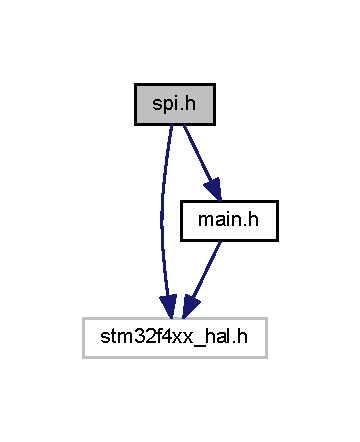
\includegraphics[width=173pt]{spi_8h__incl}
\end{center}
\end{figure}
This graph shows which files directly or indirectly include this file\+:\nopagebreak
\begin{figure}[H]
\begin{center}
\leavevmode
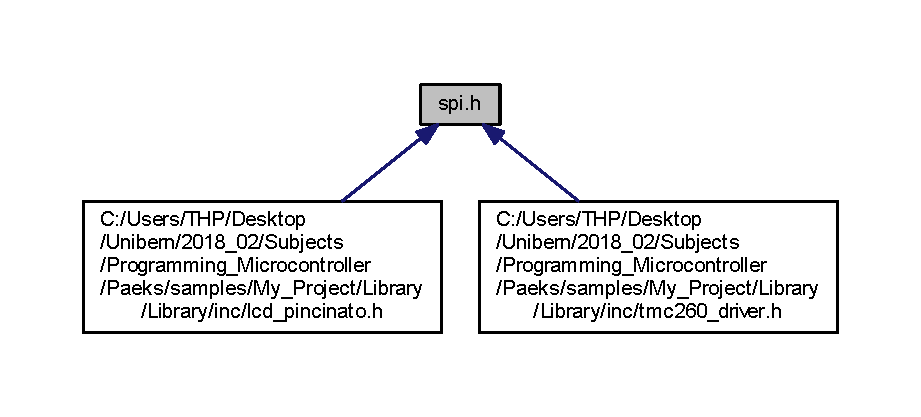
\includegraphics[width=350pt]{spi_8h__dep__incl}
\end{center}
\end{figure}
\subsection*{Functions}
\begin{DoxyCompactItemize}
\item 
void \mbox{\hyperlink{spi_8h_a47642651029b93e3f9c9edad46bd27b4}{\+\_\+\+Error\+\_\+\+Handler}} (char $\ast$, int)
\item 
void \mbox{\hyperlink{spi_8h_af81398f9775695df0b172367651ca3e6}{M\+X\+\_\+\+S\+P\+I1\+\_\+\+Init}} (void)
\item 
void \mbox{\hyperlink{spi_8h_aea85daa666c03d85fd59edef711ebb08}{M\+X\+\_\+\+S\+P\+I2\+\_\+\+Init}} (void)
\end{DoxyCompactItemize}
\subsection*{Variables}
\begin{DoxyCompactItemize}
\item 
S\+P\+I\+\_\+\+Handle\+Type\+Def \mbox{\hyperlink{spi_8h_a9c6222bae4d0328dd843ae099623b40b}{hspi1}}
\item 
S\+P\+I\+\_\+\+Handle\+Type\+Def \mbox{\hyperlink{spi_8h_ab9da65f935e805137e2eb4e18c5ab224}{hspi2}}
\end{DoxyCompactItemize}


\subsection{Function Documentation}
\mbox{\Hypertarget{spi_8h_a47642651029b93e3f9c9edad46bd27b4}\label{spi_8h_a47642651029b93e3f9c9edad46bd27b4}} 
\index{spi.\+h@{spi.\+h}!\+\_\+\+Error\+\_\+\+Handler@{\+\_\+\+Error\+\_\+\+Handler}}
\index{\+\_\+\+Error\+\_\+\+Handler@{\+\_\+\+Error\+\_\+\+Handler}!spi.\+h@{spi.\+h}}
\subsubsection{\texorpdfstring{\+\_\+\+Error\+\_\+\+Handler()}{\_Error\_Handler()}}
{\footnotesize\ttfamily void \+\_\+\+Error\+\_\+\+Handler (\begin{DoxyParamCaption}\item[{char $\ast$}]{,  }\item[{int}]{ }\end{DoxyParamCaption})}

\mbox{\Hypertarget{spi_8h_af81398f9775695df0b172367651ca3e6}\label{spi_8h_af81398f9775695df0b172367651ca3e6}} 
\index{spi.\+h@{spi.\+h}!M\+X\+\_\+\+S\+P\+I1\+\_\+\+Init@{M\+X\+\_\+\+S\+P\+I1\+\_\+\+Init}}
\index{M\+X\+\_\+\+S\+P\+I1\+\_\+\+Init@{M\+X\+\_\+\+S\+P\+I1\+\_\+\+Init}!spi.\+h@{spi.\+h}}
\subsubsection{\texorpdfstring{M\+X\+\_\+\+S\+P\+I1\+\_\+\+Init()}{MX\_SPI1\_Init()}}
{\footnotesize\ttfamily void M\+X\+\_\+\+S\+P\+I1\+\_\+\+Init (\begin{DoxyParamCaption}\item[{void}]{ }\end{DoxyParamCaption})}

\mbox{\Hypertarget{spi_8h_aea85daa666c03d85fd59edef711ebb08}\label{spi_8h_aea85daa666c03d85fd59edef711ebb08}} 
\index{spi.\+h@{spi.\+h}!M\+X\+\_\+\+S\+P\+I2\+\_\+\+Init@{M\+X\+\_\+\+S\+P\+I2\+\_\+\+Init}}
\index{M\+X\+\_\+\+S\+P\+I2\+\_\+\+Init@{M\+X\+\_\+\+S\+P\+I2\+\_\+\+Init}!spi.\+h@{spi.\+h}}
\subsubsection{\texorpdfstring{M\+X\+\_\+\+S\+P\+I2\+\_\+\+Init()}{MX\_SPI2\_Init()}}
{\footnotesize\ttfamily void M\+X\+\_\+\+S\+P\+I2\+\_\+\+Init (\begin{DoxyParamCaption}\item[{void}]{ }\end{DoxyParamCaption})}



\subsection{Variable Documentation}
\mbox{\Hypertarget{spi_8h_a9c6222bae4d0328dd843ae099623b40b}\label{spi_8h_a9c6222bae4d0328dd843ae099623b40b}} 
\index{spi.\+h@{spi.\+h}!hspi1@{hspi1}}
\index{hspi1@{hspi1}!spi.\+h@{spi.\+h}}
\subsubsection{\texorpdfstring{hspi1}{hspi1}}
{\footnotesize\ttfamily S\+P\+I\+\_\+\+Handle\+Type\+Def hspi1}

File Name \+: \mbox{\hyperlink{spi_8h}{S\+P\+I.\+h}} Description \+: This file provides code for the configuration of the S\+PI instances.

This notice applies to any and all portions of this file that are not between comment pairs U\+S\+ER C\+O\+DE B\+E\+G\+IN and U\+S\+ER C\+O\+DE E\+ND. Other portions of this file, whether inserted by the user or by software development tools are owned by their respective copyright owners.

Copyright (c) 2018 S\+T\+Microelectronics International N.\+V. All rights reserved.

Redistribution and use in source and binary forms, with or without modification, are permitted, provided that the following conditions are met\+:


\begin{DoxyEnumerate}
\item Redistribution of source code must retain the above copyright notice, this list of conditions and the following disclaimer.
\item Redistributions in binary form must reproduce the above copyright notice, this list of conditions and the following disclaimer in the documentation and/or other materials provided with the distribution.
\item Neither the name of S\+T\+Microelectronics nor the names of other contributors to this software may be used to endorse or promote products derived from this software without specific written permission.
\item This software, including modifications and/or derivative works of this software, must execute solely and exclusively on microcontroller or microprocessor devices manufactured by or for S\+T\+Microelectronics.
\item Redistribution and use of this software other than as permitted under this license is void and will automatically terminate your rights under this license.
\end{DoxyEnumerate}

T\+H\+IS S\+O\+F\+T\+W\+A\+RE IS P\+R\+O\+V\+I\+D\+ED BY S\+T\+M\+I\+C\+R\+O\+E\+L\+E\+C\+T\+R\+O\+N\+I\+CS A\+ND C\+O\+N\+T\+R\+I\+B\+U\+T\+O\+RS \char`\"{}\+A\+S I\+S\char`\"{} A\+ND A\+NY E\+X\+P\+R\+E\+SS, I\+M\+P\+L\+I\+ED OR S\+T\+A\+T\+U\+T\+O\+RY W\+A\+R\+R\+A\+N\+T\+I\+ES, I\+N\+C\+L\+U\+D\+I\+NG, B\+UT N\+OT L\+I\+M\+I\+T\+ED TO, T\+HE I\+M\+P\+L\+I\+ED W\+A\+R\+R\+A\+N\+T\+I\+ES OF M\+E\+R\+C\+H\+A\+N\+T\+A\+B\+I\+L\+I\+TY, F\+I\+T\+N\+E\+SS F\+OR A P\+A\+R\+T\+I\+C\+U\+L\+AR P\+U\+R\+P\+O\+SE A\+ND N\+O\+N-\/\+I\+N\+F\+R\+I\+N\+G\+E\+M\+E\+NT OF T\+H\+I\+RD P\+A\+R\+TY I\+N\+T\+E\+L\+L\+E\+C\+T\+U\+AL P\+R\+O\+P\+E\+R\+TY R\+I\+G\+H\+TS A\+RE D\+I\+S\+C\+L\+A\+I\+M\+ED TO T\+HE F\+U\+L\+L\+E\+ST E\+X\+T\+E\+NT P\+E\+R\+M\+I\+T\+T\+ED BY L\+AW. IN NO E\+V\+E\+NT S\+H\+A\+LL S\+T\+M\+I\+C\+R\+O\+E\+L\+E\+C\+T\+R\+O\+N\+I\+CS OR C\+O\+N\+T\+R\+I\+B\+U\+T\+O\+RS BE L\+I\+A\+B\+LE F\+OR A\+NY D\+I\+R\+E\+CT, I\+N\+D\+I\+R\+E\+CT, I\+N\+C\+I\+D\+E\+N\+T\+AL, S\+P\+E\+C\+I\+AL, E\+X\+E\+M\+P\+L\+A\+RY, OR C\+O\+N\+S\+E\+Q\+U\+E\+N\+T\+I\+AL D\+A\+M\+A\+G\+ES (I\+N\+C\+L\+U\+D\+I\+NG, B\+UT N\+OT L\+I\+M\+I\+T\+ED TO, P\+R\+O\+C\+U\+R\+E\+M\+E\+NT OF S\+U\+B\+S\+T\+I\+T\+U\+TE G\+O\+O\+DS OR S\+E\+R\+V\+I\+C\+ES; L\+O\+SS OF U\+SE, D\+A\+TA, OR P\+R\+O\+F\+I\+TS; OR B\+U\+S\+I\+N\+E\+SS I\+N\+T\+E\+R\+R\+U\+P\+T\+I\+ON) H\+O\+W\+E\+V\+ER C\+A\+U\+S\+ED A\+ND ON A\+NY T\+H\+E\+O\+RY OF L\+I\+A\+B\+I\+L\+I\+TY, W\+H\+E\+T\+H\+ER IN C\+O\+N\+T\+R\+A\+CT, S\+T\+R\+I\+CT L\+I\+A\+B\+I\+L\+I\+TY, OR T\+O\+RT (I\+N\+C\+L\+U\+D\+I\+NG N\+E\+G\+L\+I\+G\+E\+N\+CE OR O\+T\+H\+E\+R\+W\+I\+SE) A\+R\+I\+S\+I\+NG IN A\+NY W\+AY O\+UT OF T\+HE U\+SE OF T\+H\+IS S\+O\+F\+T\+W\+A\+RE, E\+V\+EN IF A\+D\+V\+I\+S\+ED OF T\+HE P\+O\+S\+S\+I\+B\+I\+L\+I\+TY OF S\+U\+CH D\+A\+M\+A\+GE. \mbox{\Hypertarget{spi_8h_ab9da65f935e805137e2eb4e18c5ab224}\label{spi_8h_ab9da65f935e805137e2eb4e18c5ab224}} 
\index{spi.\+h@{spi.\+h}!hspi2@{hspi2}}
\index{hspi2@{hspi2}!spi.\+h@{spi.\+h}}
\subsubsection{\texorpdfstring{hspi2}{hspi2}}
{\footnotesize\ttfamily S\+P\+I\+\_\+\+Handle\+Type\+Def hspi2}


\hypertarget{stm32f4xx__hal__conf_8h}{}\section{stm32f4xx\+\_\+hal\+\_\+conf.\+h File Reference}
\label{stm32f4xx__hal__conf_8h}\index{stm32f4xx\+\_\+hal\+\_\+conf.\+h@{stm32f4xx\+\_\+hal\+\_\+conf.\+h}}


H\+AL configuration file.  


{\ttfamily \#include \char`\"{}main.\+h\char`\"{}}\newline
{\ttfamily \#include \char`\"{}stm32f4xx\+\_\+hal\+\_\+rcc.\+h\char`\"{}}\newline
{\ttfamily \#include \char`\"{}stm32f4xx\+\_\+hal\+\_\+gpio.\+h\char`\"{}}\newline
{\ttfamily \#include \char`\"{}stm32f4xx\+\_\+hal\+\_\+dma.\+h\char`\"{}}\newline
{\ttfamily \#include \char`\"{}stm32f4xx\+\_\+hal\+\_\+cortex.\+h\char`\"{}}\newline
{\ttfamily \#include \char`\"{}stm32f4xx\+\_\+hal\+\_\+adc.\+h\char`\"{}}\newline
{\ttfamily \#include \char`\"{}stm32f4xx\+\_\+hal\+\_\+flash.\+h\char`\"{}}\newline
{\ttfamily \#include \char`\"{}stm32f4xx\+\_\+hal\+\_\+i2c.\+h\char`\"{}}\newline
{\ttfamily \#include \char`\"{}stm32f4xx\+\_\+hal\+\_\+pwr.\+h\char`\"{}}\newline
{\ttfamily \#include \char`\"{}stm32f4xx\+\_\+hal\+\_\+spi.\+h\char`\"{}}\newline
{\ttfamily \#include \char`\"{}stm32f4xx\+\_\+hal\+\_\+tim.\+h\char`\"{}}\newline
{\ttfamily \#include \char`\"{}stm32f4xx\+\_\+hal\+\_\+uart.\+h\char`\"{}}\newline
Include dependency graph for stm32f4xx\+\_\+hal\+\_\+conf.\+h\+:\nopagebreak
\begin{figure}[H]
\begin{center}
\leavevmode
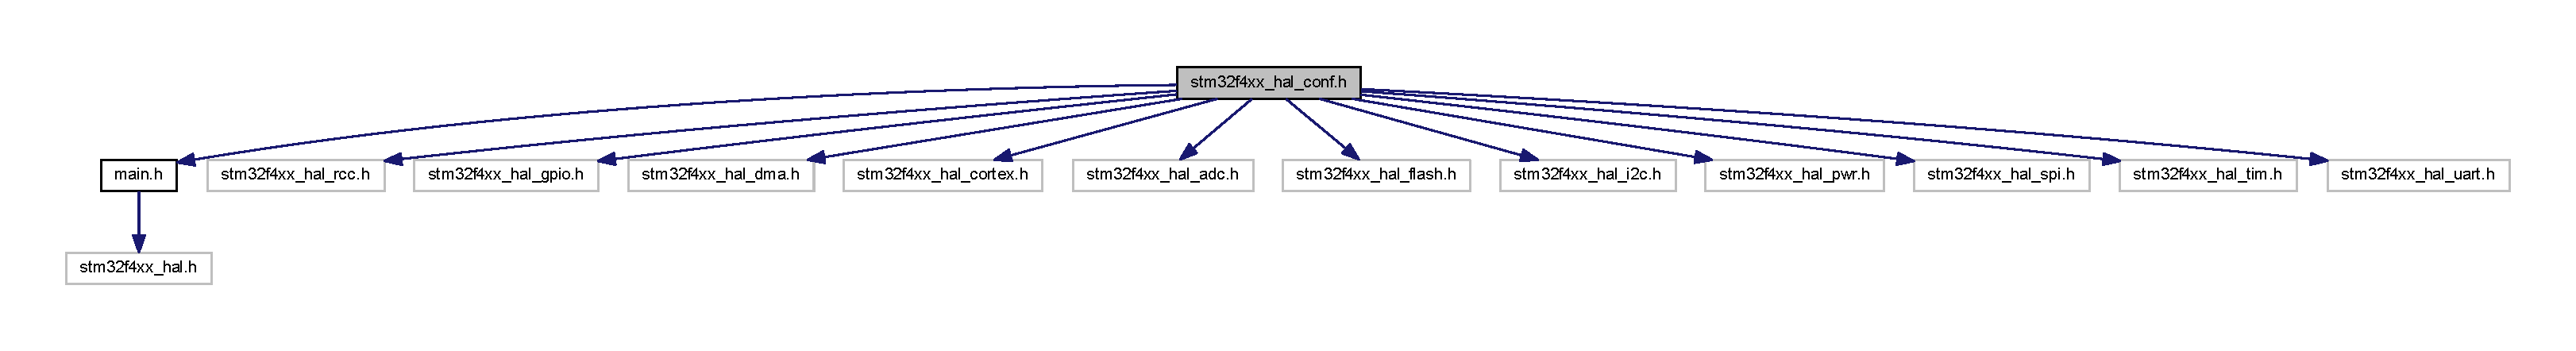
\includegraphics[width=350pt]{stm32f4xx__hal__conf_8h__incl}
\end{center}
\end{figure}
\subsection*{Macros}
\begin{DoxyCompactItemize}
\item 
\#define \mbox{\hyperlink{stm32f4xx__hal__conf_8h_a877ae99e8c47a609ea97c888912bf75f}{H\+A\+L\+\_\+\+M\+O\+D\+U\+L\+E\+\_\+\+E\+N\+A\+B\+L\+ED}}
\begin{DoxyCompactList}\small\item\em This is the list of modules to be used in the H\+AL driver. \end{DoxyCompactList}\item 
\#define \mbox{\hyperlink{stm32f4xx__hal__conf_8h_a476f1655c969ae57e89a74d98c75f43f}{H\+A\+L\+\_\+\+A\+D\+C\+\_\+\+M\+O\+D\+U\+L\+E\+\_\+\+E\+N\+A\+B\+L\+ED}}
\item 
\#define \mbox{\hyperlink{stm32f4xx__hal__conf_8h_a19999766418b0224871f732d800841c6}{H\+A\+L\+\_\+\+I2\+C\+\_\+\+M\+O\+D\+U\+L\+E\+\_\+\+E\+N\+A\+B\+L\+ED}}
\item 
\#define \mbox{\hyperlink{stm32f4xx__hal__conf_8h_a8ad4712bf4add56892d057778e826e0c}{H\+A\+L\+\_\+\+S\+P\+I\+\_\+\+M\+O\+D\+U\+L\+E\+\_\+\+E\+N\+A\+B\+L\+ED}}
\item 
\#define \mbox{\hyperlink{stm32f4xx__hal__conf_8h_a23382b8f04b3e6db2c59dfa1ef5ea4a2}{H\+A\+L\+\_\+\+T\+I\+M\+\_\+\+M\+O\+D\+U\+L\+E\+\_\+\+E\+N\+A\+B\+L\+ED}}
\item 
\#define \mbox{\hyperlink{stm32f4xx__hal__conf_8h_a167269406e73327b95c3bb7b9cfe6d89}{H\+A\+L\+\_\+\+U\+A\+R\+T\+\_\+\+M\+O\+D\+U\+L\+E\+\_\+\+E\+N\+A\+B\+L\+ED}}
\item 
\#define \mbox{\hyperlink{stm32f4xx__hal__conf_8h_a86165f80d6078719ee0715afe13febf5}{H\+A\+L\+\_\+\+G\+P\+I\+O\+\_\+\+M\+O\+D\+U\+L\+E\+\_\+\+E\+N\+A\+B\+L\+ED}}
\item 
\#define \mbox{\hyperlink{stm32f4xx__hal__conf_8h_a6552186102a1131b2849ac55a582945d}{H\+A\+L\+\_\+\+D\+M\+A\+\_\+\+M\+O\+D\+U\+L\+E\+\_\+\+E\+N\+A\+B\+L\+ED}}
\item 
\#define \mbox{\hyperlink{stm32f4xx__hal__conf_8h_ac3dd74314ed62ac8575e2f9f48b3ac48}{H\+A\+L\+\_\+\+R\+C\+C\+\_\+\+M\+O\+D\+U\+L\+E\+\_\+\+E\+N\+A\+B\+L\+ED}}
\item 
\#define \mbox{\hyperlink{stm32f4xx__hal__conf_8h_a7112575efe3740911f19a13e6b170fee}{H\+A\+L\+\_\+\+F\+L\+A\+S\+H\+\_\+\+M\+O\+D\+U\+L\+E\+\_\+\+E\+N\+A\+B\+L\+ED}}
\item 
\#define \mbox{\hyperlink{stm32f4xx__hal__conf_8h_ab51923c3716977d7923f49cc9d081aa8}{H\+A\+L\+\_\+\+P\+W\+R\+\_\+\+M\+O\+D\+U\+L\+E\+\_\+\+E\+N\+A\+B\+L\+ED}}
\item 
\#define \mbox{\hyperlink{stm32f4xx__hal__conf_8h_aa9b5a3a425901e097de70092dbe31e0f}{H\+A\+L\+\_\+\+C\+O\+R\+T\+E\+X\+\_\+\+M\+O\+D\+U\+L\+E\+\_\+\+E\+N\+A\+B\+L\+ED}}
\item 
\#define \mbox{\hyperlink{stm32f4xx__hal__conf_8h_aeafcff4f57440c60e64812dddd13e7cb}{H\+S\+E\+\_\+\+V\+A\+L\+UE}}~((uint32\+\_\+t)25000000\+U)
\begin{DoxyCompactList}\small\item\em Adjust the value of External High Speed oscillator (H\+SE) used in your application. This value is used by the R\+CC H\+AL module to compute the system frequency (when H\+SE is used as system clock source, directly or through the P\+LL). ~\newline
~\newline
 \end{DoxyCompactList}\item 
\#define \mbox{\hyperlink{stm32f4xx__hal__conf_8h_a68ecbc9b0a1a40a1ec9d18d5e9747c4f}{H\+S\+E\+\_\+\+S\+T\+A\+R\+T\+U\+P\+\_\+\+T\+I\+M\+E\+O\+UT}}~((uint32\+\_\+t)100\+U)
\item 
\#define \mbox{\hyperlink{stm32f4xx__hal__conf_8h_aaa8c76e274d0f6dd2cefb5d0b17fbc37}{H\+S\+I\+\_\+\+V\+A\+L\+UE}}~((uint32\+\_\+t)16000000\+U)
\begin{DoxyCompactList}\small\item\em Internal High Speed oscillator (H\+SI) value. This value is used by the R\+CC H\+AL module to compute the system frequency (when H\+SI is used as system clock source, directly or through the P\+LL). \end{DoxyCompactList}\item 
\#define \mbox{\hyperlink{stm32f4xx__hal__conf_8h_a4872023e65449c0506aac3ea6bec99e9}{L\+S\+I\+\_\+\+V\+A\+L\+UE}}~((uint32\+\_\+t)32000\+U)
\begin{DoxyCompactList}\small\item\em Internal Low Speed oscillator (L\+SI) value. \end{DoxyCompactList}\item 
\#define \mbox{\hyperlink{stm32f4xx__hal__conf_8h_a7bbb9d19e5189a6ccd0fb6fa6177d20d}{L\+S\+E\+\_\+\+V\+A\+L\+UE}}~((uint32\+\_\+t)32768\+U)
\begin{DoxyCompactList}\small\item\em External Low Speed oscillator (L\+SE) value. \end{DoxyCompactList}\item 
\#define \mbox{\hyperlink{stm32f4xx__hal__conf_8h_a85e6fc812dc26f7161a04be2568a5462}{L\+S\+E\+\_\+\+S\+T\+A\+R\+T\+U\+P\+\_\+\+T\+I\+M\+E\+O\+UT}}~((uint32\+\_\+t)5000\+U)
\item 
\#define \mbox{\hyperlink{stm32f4xx__hal__conf_8h_a8c47c935e91e70569098b41718558648}{E\+X\+T\+E\+R\+N\+A\+L\+\_\+\+C\+L\+O\+C\+K\+\_\+\+V\+A\+L\+UE}}~((uint32\+\_\+t)12288000\+U)
\begin{DoxyCompactList}\small\item\em External clock source for I2S peripheral This value is used by the I2S H\+AL module to compute the I2S clock source frequency, this source is inserted directly through I2\+S\+\_\+\+C\+K\+IN pad. \end{DoxyCompactList}\item 
\#define \mbox{\hyperlink{stm32f4xx__hal__conf_8h_aae550dad9f96d52cfce5e539adadbbb4}{V\+D\+D\+\_\+\+V\+A\+L\+UE}}~((uint32\+\_\+t)3300\+U)
\begin{DoxyCompactList}\small\item\em This is the H\+AL system configuration section. \end{DoxyCompactList}\item 
\#define \mbox{\hyperlink{stm32f4xx__hal__conf_8h_ae27809d4959b9fd5b5d974e3e1c77d2e}{T\+I\+C\+K\+\_\+\+I\+N\+T\+\_\+\+P\+R\+I\+O\+R\+I\+TY}}~((uint32\+\_\+t)0\+U)
\item 
\#define \mbox{\hyperlink{stm32f4xx__hal__conf_8h_ad048ac737242c2c2cb9f4a72953d10ce}{U\+S\+E\+\_\+\+R\+T\+OS}}~0U
\item 
\#define \mbox{\hyperlink{stm32f4xx__hal__conf_8h_a13fc0d5e7bb925385c0cc0772ba6a391}{P\+R\+E\+F\+E\+T\+C\+H\+\_\+\+E\+N\+A\+B\+LE}}~1U
\item 
\#define \mbox{\hyperlink{stm32f4xx__hal__conf_8h_a3379989d46599c7e19a43f42e9145a4a}{I\+N\+S\+T\+R\+U\+C\+T\+I\+O\+N\+\_\+\+C\+A\+C\+H\+E\+\_\+\+E\+N\+A\+B\+LE}}~1U
\item 
\#define \mbox{\hyperlink{stm32f4xx__hal__conf_8h_a5b4c32a40cf49b06c0d761e385949a6b}{D\+A\+T\+A\+\_\+\+C\+A\+C\+H\+E\+\_\+\+E\+N\+A\+B\+LE}}~1U
\item 
\#define \mbox{\hyperlink{stm32f4xx__hal__conf_8h_ab84a2e15d360e2644ada09641513a941}{M\+A\+C\+\_\+\+A\+D\+D\+R0}}~2U
\begin{DoxyCompactList}\small\item\em Uncomment the line below to expanse the \char`\"{}assert\+\_\+param\char`\"{} macro in the H\+AL drivers code. \end{DoxyCompactList}\item 
\#define \mbox{\hyperlink{stm32f4xx__hal__conf_8h_a8d14266d76690c530bee01e7e5bb4099}{M\+A\+C\+\_\+\+A\+D\+D\+R1}}~0U
\item 
\#define \mbox{\hyperlink{stm32f4xx__hal__conf_8h_a6c5df15bec1d305ed033ad9a85ec803d}{M\+A\+C\+\_\+\+A\+D\+D\+R2}}~0U
\item 
\#define \mbox{\hyperlink{stm32f4xx__hal__conf_8h_a08a36ede83ae67498aecf54676be8fc8}{M\+A\+C\+\_\+\+A\+D\+D\+R3}}~0U
\item 
\#define \mbox{\hyperlink{stm32f4xx__hal__conf_8h_a41e5cb0b39ad74f0aafb83dbcecf9006}{M\+A\+C\+\_\+\+A\+D\+D\+R4}}~0U
\item 
\#define \mbox{\hyperlink{stm32f4xx__hal__conf_8h_a3bcc92663c42ec434f527847bbc4abc1}{M\+A\+C\+\_\+\+A\+D\+D\+R5}}~0U
\item 
\#define \mbox{\hyperlink{stm32f4xx__hal__conf_8h_a0cdaf687f7a7f2dba570d5a722990786}{E\+T\+H\+\_\+\+R\+X\+\_\+\+B\+U\+F\+\_\+\+S\+I\+ZE}}~E\+T\+H\+\_\+\+M\+A\+X\+\_\+\+P\+A\+C\+K\+E\+T\+\_\+\+S\+I\+ZE /$\ast$ buffer size for receive               $\ast$/
\item 
\#define \mbox{\hyperlink{stm32f4xx__hal__conf_8h_af83956dfc1b135c3c92ac409758b6cf4}{E\+T\+H\+\_\+\+T\+X\+\_\+\+B\+U\+F\+\_\+\+S\+I\+ZE}}~E\+T\+H\+\_\+\+M\+A\+X\+\_\+\+P\+A\+C\+K\+E\+T\+\_\+\+S\+I\+ZE /$\ast$ buffer size for transmit              $\ast$/
\item 
\#define \mbox{\hyperlink{stm32f4xx__hal__conf_8h_a62b0f224fa9c4f2e5574c9e52526f751}{E\+T\+H\+\_\+\+R\+X\+B\+U\+F\+NB}}~((uint32\+\_\+t)4\+U)       /$\ast$ 4 Rx buffers of size E\+T\+H\+\_\+\+R\+X\+\_\+\+B\+U\+F\+\_\+\+S\+I\+Z\+E  $\ast$/
\item 
\#define \mbox{\hyperlink{stm32f4xx__hal__conf_8h_a4ad07ad8fa6f8639ab8ef362390d86c7}{E\+T\+H\+\_\+\+T\+X\+B\+U\+F\+NB}}~((uint32\+\_\+t)4\+U)       /$\ast$ 4 Tx buffers of size E\+T\+H\+\_\+\+T\+X\+\_\+\+B\+U\+F\+\_\+\+S\+I\+Z\+E  $\ast$/
\item 
\#define \mbox{\hyperlink{stm32f4xx__hal__conf_8h_a25f014091aaba92bdd9d95d0b2f00503}{D\+P83848\+\_\+\+P\+H\+Y\+\_\+\+A\+D\+D\+R\+E\+SS}}~0x01U
\item 
\#define \mbox{\hyperlink{stm32f4xx__hal__conf_8h_a0ede6087f7b71403bcddb5d3a8f47ff4}{P\+H\+Y\+\_\+\+R\+E\+S\+E\+T\+\_\+\+D\+E\+L\+AY}}~((uint32\+\_\+t)0x000000\+F\+F\+U)
\item 
\#define \mbox{\hyperlink{stm32f4xx__hal__conf_8h_abba7114255a2a41b81fdcb2a3702c270}{P\+H\+Y\+\_\+\+C\+O\+N\+F\+I\+G\+\_\+\+D\+E\+L\+AY}}~((uint32\+\_\+t)0x00000\+F\+F\+F\+U)
\item 
\#define \mbox{\hyperlink{stm32f4xx__hal__conf_8h_a9d356ada86535630c403690bef0fb887}{P\+H\+Y\+\_\+\+R\+E\+A\+D\+\_\+\+TO}}~((uint32\+\_\+t)0x0000\+F\+F\+F\+F\+U)
\item 
\#define \mbox{\hyperlink{stm32f4xx__hal__conf_8h_a474bf13e28d09b667e41b151140ee39d}{P\+H\+Y\+\_\+\+W\+R\+I\+T\+E\+\_\+\+TO}}~((uint32\+\_\+t)0x0000\+F\+F\+F\+F\+U)
\item 
\#define \mbox{\hyperlink{stm32f4xx__hal__conf_8h_a8abe1a40c71e68881ec669d59f513fdb}{P\+H\+Y\+\_\+\+B\+CR}}~((uint16\+\_\+t)0x0000\+U)
\item 
\#define \mbox{\hyperlink{stm32f4xx__hal__conf_8h_a4b8f2c29a9e74412395e1b1809666838}{P\+H\+Y\+\_\+\+B\+SR}}~((uint16\+\_\+t)0x0001\+U)
\item 
\#define \mbox{\hyperlink{stm32f4xx__hal__conf_8h_a6f5048620b3dde8583f7f1118e9de187}{P\+H\+Y\+\_\+\+R\+E\+S\+ET}}~((uint16\+\_\+t)0x8000\+U)
\item 
\#define \mbox{\hyperlink{stm32f4xx__hal__conf_8h_a7833d885caa7e29abbebfb90a4b96f86}{P\+H\+Y\+\_\+\+L\+O\+O\+P\+B\+A\+CK}}~((uint16\+\_\+t)0x4000\+U)
\item 
\#define \mbox{\hyperlink{stm32f4xx__hal__conf_8h_a5729771244f68779fc694ba819cd60a5}{P\+H\+Y\+\_\+\+F\+U\+L\+L\+D\+U\+P\+L\+E\+X\+\_\+100M}}~((uint16\+\_\+t)0x2100\+U)
\item 
\#define \mbox{\hyperlink{stm32f4xx__hal__conf_8h_a1ac901a4ad405241d90a5c10104b8986}{P\+H\+Y\+\_\+\+H\+A\+L\+F\+D\+U\+P\+L\+E\+X\+\_\+100M}}~((uint16\+\_\+t)0x2000\+U)
\item 
\#define \mbox{\hyperlink{stm32f4xx__hal__conf_8h_a6b6254fd3dacbf1578a9d8058cd86373}{P\+H\+Y\+\_\+\+F\+U\+L\+L\+D\+U\+P\+L\+E\+X\+\_\+10M}}~((uint16\+\_\+t)0x0100\+U)
\item 
\#define \mbox{\hyperlink{stm32f4xx__hal__conf_8h_a4fa7ca6faf60ee074576ebb6103f8dd4}{P\+H\+Y\+\_\+\+H\+A\+L\+F\+D\+U\+P\+L\+E\+X\+\_\+10M}}~((uint16\+\_\+t)0x0000\+U)
\item 
\#define \mbox{\hyperlink{stm32f4xx__hal__conf_8h_a9b7f5c8f71047ee449f21562d26b1b43}{P\+H\+Y\+\_\+\+A\+U\+T\+O\+N\+E\+G\+O\+T\+I\+A\+T\+I\+ON}}~((uint16\+\_\+t)0x1000\+U)
\item 
\#define \mbox{\hyperlink{stm32f4xx__hal__conf_8h_a66c4b69bd08dc25b6730365d3ff740c9}{P\+H\+Y\+\_\+\+R\+E\+S\+T\+A\+R\+T\+\_\+\+A\+U\+T\+O\+N\+E\+G\+O\+T\+I\+A\+T\+I\+ON}}~((uint16\+\_\+t)0x0200\+U)
\item 
\#define \mbox{\hyperlink{stm32f4xx__hal__conf_8h_aa0b1e6d4a23470fc1ac4f9222b51f8a0}{P\+H\+Y\+\_\+\+P\+O\+W\+E\+R\+D\+O\+WN}}~((uint16\+\_\+t)0x0800\+U)
\item 
\#define \mbox{\hyperlink{stm32f4xx__hal__conf_8h_a7d5233295134a385866eb5bdafe2162b}{P\+H\+Y\+\_\+\+I\+S\+O\+L\+A\+TE}}~((uint16\+\_\+t)0x0400\+U)
\item 
\#define \mbox{\hyperlink{stm32f4xx__hal__conf_8h_a36c4dbd5f6df1f5eaefa010929ef9773}{P\+H\+Y\+\_\+\+A\+U\+T\+O\+N\+E\+G\+O\+\_\+\+C\+O\+M\+P\+L\+E\+TE}}~((uint16\+\_\+t)0x0020\+U)
\item 
\#define \mbox{\hyperlink{stm32f4xx__hal__conf_8h_ace209074499dbef0b97300da5bd7c707}{P\+H\+Y\+\_\+\+L\+I\+N\+K\+E\+D\+\_\+\+S\+T\+A\+T\+US}}~((uint16\+\_\+t)0x0004\+U)
\item 
\#define \mbox{\hyperlink{stm32f4xx__hal__conf_8h_a057b4d3fb66548d65c291a5b41611be2}{P\+H\+Y\+\_\+\+J\+A\+B\+B\+E\+R\+\_\+\+D\+E\+T\+E\+C\+T\+I\+ON}}~((uint16\+\_\+t)0x0002\+U)
\item 
\#define \mbox{\hyperlink{stm32f4xx__hal__conf_8h_a32b55e84d27cf298a77f54b133cd1acc}{P\+H\+Y\+\_\+\+SR}}~((uint16\+\_\+t)0x10\+U)
\item 
\#define \mbox{\hyperlink{stm32f4xx__hal__conf_8h_a74c081bc55e9ff96bf229f44e96c6155}{P\+H\+Y\+\_\+\+S\+P\+E\+E\+D\+\_\+\+S\+T\+A\+T\+US}}~((uint16\+\_\+t)0x0002\+U)
\item 
\#define \mbox{\hyperlink{stm32f4xx__hal__conf_8h_ab928f45585242fde1a8d81a2d9ed22d0}{P\+H\+Y\+\_\+\+D\+U\+P\+L\+E\+X\+\_\+\+S\+T\+A\+T\+US}}~((uint16\+\_\+t)0x0004\+U)
\item 
\#define \mbox{\hyperlink{stm32f4xx__hal__conf_8h_a4c6fab687afc7ba4469b1b2d34472358}{U\+S\+E\+\_\+\+S\+P\+I\+\_\+\+C\+RC}}~0U
\item 
\#define \mbox{\hyperlink{stm32f4xx__hal__conf_8h_a631dea7b230e600555f979c62af1de21}{assert\+\_\+param}}(expr)~((void)0\+U)
\begin{DoxyCompactList}\small\item\em Include module\textquotesingle{}s header file. \end{DoxyCompactList}\end{DoxyCompactItemize}


\subsection{Detailed Description}
H\+AL configuration file. 

\begin{DoxyAttention}{Attention}

\end{DoxyAttention}
\subsubsection*{\begin{center}\copyright{} C\+O\+P\+Y\+R\+I\+G\+H\+T(c) 2018 S\+T\+Microelectronics\end{center} }

Redistribution and use in source and binary forms, with or without modification, are permitted provided that the following conditions are met\+:
\begin{DoxyEnumerate}
\item Redistributions of source code must retain the above copyright notice, this list of conditions and the following disclaimer.
\item Redistributions in binary form must reproduce the above copyright notice, this list of conditions and the following disclaimer in the documentation and/or other materials provided with the distribution.
\item Neither the name of S\+T\+Microelectronics nor the names of its contributors may be used to endorse or promote products derived from this software without specific prior written permission.
\end{DoxyEnumerate}

T\+H\+IS S\+O\+F\+T\+W\+A\+RE IS P\+R\+O\+V\+I\+D\+ED BY T\+HE C\+O\+P\+Y\+R\+I\+G\+HT H\+O\+L\+D\+E\+RS A\+ND C\+O\+N\+T\+R\+I\+B\+U\+T\+O\+RS \char`\"{}\+A\+S I\+S\char`\"{} A\+ND A\+NY E\+X\+P\+R\+E\+SS OR I\+M\+P\+L\+I\+ED W\+A\+R\+R\+A\+N\+T\+I\+ES, I\+N\+C\+L\+U\+D\+I\+NG, B\+UT N\+OT L\+I\+M\+I\+T\+ED TO, T\+HE I\+M\+P\+L\+I\+ED W\+A\+R\+R\+A\+N\+T\+I\+ES OF M\+E\+R\+C\+H\+A\+N\+T\+A\+B\+I\+L\+I\+TY A\+ND F\+I\+T\+N\+E\+SS F\+OR A P\+A\+R\+T\+I\+C\+U\+L\+AR P\+U\+R\+P\+O\+SE A\+RE D\+I\+S\+C\+L\+A\+I\+M\+ED. IN NO E\+V\+E\+NT S\+H\+A\+LL T\+HE C\+O\+P\+Y\+R\+I\+G\+HT H\+O\+L\+D\+ER OR C\+O\+N\+T\+R\+I\+B\+U\+T\+O\+RS BE L\+I\+A\+B\+LE F\+OR A\+NY D\+I\+R\+E\+CT, I\+N\+D\+I\+R\+E\+CT, I\+N\+C\+I\+D\+E\+N\+T\+AL, S\+P\+E\+C\+I\+AL, E\+X\+E\+M\+P\+L\+A\+RY, OR C\+O\+N\+S\+E\+Q\+U\+E\+N\+T\+I\+AL D\+A\+M\+A\+G\+ES (I\+N\+C\+L\+U\+D\+I\+NG, B\+UT N\+OT L\+I\+M\+I\+T\+ED TO, P\+R\+O\+C\+U\+R\+E\+M\+E\+NT OF S\+U\+B\+S\+T\+I\+T\+U\+TE G\+O\+O\+DS OR S\+E\+R\+V\+I\+C\+ES; L\+O\+SS OF U\+SE, D\+A\+TA, OR P\+R\+O\+F\+I\+TS; OR B\+U\+S\+I\+N\+E\+SS I\+N\+T\+E\+R\+R\+U\+P\+T\+I\+ON) H\+O\+W\+E\+V\+ER C\+A\+U\+S\+ED A\+ND ON A\+NY T\+H\+E\+O\+RY OF L\+I\+A\+B\+I\+L\+I\+TY, W\+H\+E\+T\+H\+ER IN C\+O\+N\+T\+R\+A\+CT, S\+T\+R\+I\+CT L\+I\+A\+B\+I\+L\+I\+TY, OR T\+O\+RT (I\+N\+C\+L\+U\+D\+I\+NG N\+E\+G\+L\+I\+G\+E\+N\+CE OR O\+T\+H\+E\+R\+W\+I\+SE) A\+R\+I\+S\+I\+NG IN A\+NY W\+AY O\+UT OF T\+HE U\+SE OF T\+H\+IS S\+O\+F\+T\+W\+A\+RE, E\+V\+EN IF A\+D\+V\+I\+S\+ED OF T\+HE P\+O\+S\+S\+I\+B\+I\+L\+I\+TY OF S\+U\+CH D\+A\+M\+A\+GE. 

\subsection{Macro Definition Documentation}
\mbox{\Hypertarget{stm32f4xx__hal__conf_8h_a631dea7b230e600555f979c62af1de21}\label{stm32f4xx__hal__conf_8h_a631dea7b230e600555f979c62af1de21}} 
\index{stm32f4xx\+\_\+hal\+\_\+conf.\+h@{stm32f4xx\+\_\+hal\+\_\+conf.\+h}!assert\+\_\+param@{assert\+\_\+param}}
\index{assert\+\_\+param@{assert\+\_\+param}!stm32f4xx\+\_\+hal\+\_\+conf.\+h@{stm32f4xx\+\_\+hal\+\_\+conf.\+h}}
\subsubsection{\texorpdfstring{assert\+\_\+param}{assert\_param}}
{\footnotesize\ttfamily \#define assert\+\_\+param(\begin{DoxyParamCaption}\item[{}]{expr }\end{DoxyParamCaption})~((void)0\+U)}



Include module\textquotesingle{}s header file. 



Definition at line 442 of file stm32f4xx\+\_\+hal\+\_\+conf.\+h.

\mbox{\Hypertarget{stm32f4xx__hal__conf_8h_a5b4c32a40cf49b06c0d761e385949a6b}\label{stm32f4xx__hal__conf_8h_a5b4c32a40cf49b06c0d761e385949a6b}} 
\index{stm32f4xx\+\_\+hal\+\_\+conf.\+h@{stm32f4xx\+\_\+hal\+\_\+conf.\+h}!D\+A\+T\+A\+\_\+\+C\+A\+C\+H\+E\+\_\+\+E\+N\+A\+B\+LE@{D\+A\+T\+A\+\_\+\+C\+A\+C\+H\+E\+\_\+\+E\+N\+A\+B\+LE}}
\index{D\+A\+T\+A\+\_\+\+C\+A\+C\+H\+E\+\_\+\+E\+N\+A\+B\+LE@{D\+A\+T\+A\+\_\+\+C\+A\+C\+H\+E\+\_\+\+E\+N\+A\+B\+LE}!stm32f4xx\+\_\+hal\+\_\+conf.\+h@{stm32f4xx\+\_\+hal\+\_\+conf.\+h}}
\subsubsection{\texorpdfstring{D\+A\+T\+A\+\_\+\+C\+A\+C\+H\+E\+\_\+\+E\+N\+A\+B\+LE}{DATA\_CACHE\_ENABLE}}
{\footnotesize\ttfamily \#define D\+A\+T\+A\+\_\+\+C\+A\+C\+H\+E\+\_\+\+E\+N\+A\+B\+LE~1U}



Definition at line 165 of file stm32f4xx\+\_\+hal\+\_\+conf.\+h.

\mbox{\Hypertarget{stm32f4xx__hal__conf_8h_a25f014091aaba92bdd9d95d0b2f00503}\label{stm32f4xx__hal__conf_8h_a25f014091aaba92bdd9d95d0b2f00503}} 
\index{stm32f4xx\+\_\+hal\+\_\+conf.\+h@{stm32f4xx\+\_\+hal\+\_\+conf.\+h}!D\+P83848\+\_\+\+P\+H\+Y\+\_\+\+A\+D\+D\+R\+E\+SS@{D\+P83848\+\_\+\+P\+H\+Y\+\_\+\+A\+D\+D\+R\+E\+SS}}
\index{D\+P83848\+\_\+\+P\+H\+Y\+\_\+\+A\+D\+D\+R\+E\+SS@{D\+P83848\+\_\+\+P\+H\+Y\+\_\+\+A\+D\+D\+R\+E\+SS}!stm32f4xx\+\_\+hal\+\_\+conf.\+h@{stm32f4xx\+\_\+hal\+\_\+conf.\+h}}
\subsubsection{\texorpdfstring{D\+P83848\+\_\+\+P\+H\+Y\+\_\+\+A\+D\+D\+R\+E\+SS}{DP83848\_PHY\_ADDRESS}}
{\footnotesize\ttfamily \#define D\+P83848\+\_\+\+P\+H\+Y\+\_\+\+A\+D\+D\+R\+E\+SS~0x01U}



Definition at line 195 of file stm32f4xx\+\_\+hal\+\_\+conf.\+h.

\mbox{\Hypertarget{stm32f4xx__hal__conf_8h_a0cdaf687f7a7f2dba570d5a722990786}\label{stm32f4xx__hal__conf_8h_a0cdaf687f7a7f2dba570d5a722990786}} 
\index{stm32f4xx\+\_\+hal\+\_\+conf.\+h@{stm32f4xx\+\_\+hal\+\_\+conf.\+h}!E\+T\+H\+\_\+\+R\+X\+\_\+\+B\+U\+F\+\_\+\+S\+I\+ZE@{E\+T\+H\+\_\+\+R\+X\+\_\+\+B\+U\+F\+\_\+\+S\+I\+ZE}}
\index{E\+T\+H\+\_\+\+R\+X\+\_\+\+B\+U\+F\+\_\+\+S\+I\+ZE@{E\+T\+H\+\_\+\+R\+X\+\_\+\+B\+U\+F\+\_\+\+S\+I\+ZE}!stm32f4xx\+\_\+hal\+\_\+conf.\+h@{stm32f4xx\+\_\+hal\+\_\+conf.\+h}}
\subsubsection{\texorpdfstring{E\+T\+H\+\_\+\+R\+X\+\_\+\+B\+U\+F\+\_\+\+S\+I\+ZE}{ETH\_RX\_BUF\_SIZE}}
{\footnotesize\ttfamily \#define E\+T\+H\+\_\+\+R\+X\+\_\+\+B\+U\+F\+\_\+\+S\+I\+ZE~E\+T\+H\+\_\+\+M\+A\+X\+\_\+\+P\+A\+C\+K\+E\+T\+\_\+\+S\+I\+ZE /$\ast$ buffer size for receive               $\ast$/}



Definition at line 187 of file stm32f4xx\+\_\+hal\+\_\+conf.\+h.

\mbox{\Hypertarget{stm32f4xx__hal__conf_8h_a62b0f224fa9c4f2e5574c9e52526f751}\label{stm32f4xx__hal__conf_8h_a62b0f224fa9c4f2e5574c9e52526f751}} 
\index{stm32f4xx\+\_\+hal\+\_\+conf.\+h@{stm32f4xx\+\_\+hal\+\_\+conf.\+h}!E\+T\+H\+\_\+\+R\+X\+B\+U\+F\+NB@{E\+T\+H\+\_\+\+R\+X\+B\+U\+F\+NB}}
\index{E\+T\+H\+\_\+\+R\+X\+B\+U\+F\+NB@{E\+T\+H\+\_\+\+R\+X\+B\+U\+F\+NB}!stm32f4xx\+\_\+hal\+\_\+conf.\+h@{stm32f4xx\+\_\+hal\+\_\+conf.\+h}}
\subsubsection{\texorpdfstring{E\+T\+H\+\_\+\+R\+X\+B\+U\+F\+NB}{ETH\_RXBUFNB}}
{\footnotesize\ttfamily \#define E\+T\+H\+\_\+\+R\+X\+B\+U\+F\+NB~((uint32\+\_\+t)4\+U)       /$\ast$ 4 Rx buffers of size E\+T\+H\+\_\+\+R\+X\+\_\+\+B\+U\+F\+\_\+\+S\+I\+Z\+E  $\ast$/}



Definition at line 189 of file stm32f4xx\+\_\+hal\+\_\+conf.\+h.

\mbox{\Hypertarget{stm32f4xx__hal__conf_8h_af83956dfc1b135c3c92ac409758b6cf4}\label{stm32f4xx__hal__conf_8h_af83956dfc1b135c3c92ac409758b6cf4}} 
\index{stm32f4xx\+\_\+hal\+\_\+conf.\+h@{stm32f4xx\+\_\+hal\+\_\+conf.\+h}!E\+T\+H\+\_\+\+T\+X\+\_\+\+B\+U\+F\+\_\+\+S\+I\+ZE@{E\+T\+H\+\_\+\+T\+X\+\_\+\+B\+U\+F\+\_\+\+S\+I\+ZE}}
\index{E\+T\+H\+\_\+\+T\+X\+\_\+\+B\+U\+F\+\_\+\+S\+I\+ZE@{E\+T\+H\+\_\+\+T\+X\+\_\+\+B\+U\+F\+\_\+\+S\+I\+ZE}!stm32f4xx\+\_\+hal\+\_\+conf.\+h@{stm32f4xx\+\_\+hal\+\_\+conf.\+h}}
\subsubsection{\texorpdfstring{E\+T\+H\+\_\+\+T\+X\+\_\+\+B\+U\+F\+\_\+\+S\+I\+ZE}{ETH\_TX\_BUF\_SIZE}}
{\footnotesize\ttfamily \#define E\+T\+H\+\_\+\+T\+X\+\_\+\+B\+U\+F\+\_\+\+S\+I\+ZE~E\+T\+H\+\_\+\+M\+A\+X\+\_\+\+P\+A\+C\+K\+E\+T\+\_\+\+S\+I\+ZE /$\ast$ buffer size for transmit              $\ast$/}



Definition at line 188 of file stm32f4xx\+\_\+hal\+\_\+conf.\+h.

\mbox{\Hypertarget{stm32f4xx__hal__conf_8h_a4ad07ad8fa6f8639ab8ef362390d86c7}\label{stm32f4xx__hal__conf_8h_a4ad07ad8fa6f8639ab8ef362390d86c7}} 
\index{stm32f4xx\+\_\+hal\+\_\+conf.\+h@{stm32f4xx\+\_\+hal\+\_\+conf.\+h}!E\+T\+H\+\_\+\+T\+X\+B\+U\+F\+NB@{E\+T\+H\+\_\+\+T\+X\+B\+U\+F\+NB}}
\index{E\+T\+H\+\_\+\+T\+X\+B\+U\+F\+NB@{E\+T\+H\+\_\+\+T\+X\+B\+U\+F\+NB}!stm32f4xx\+\_\+hal\+\_\+conf.\+h@{stm32f4xx\+\_\+hal\+\_\+conf.\+h}}
\subsubsection{\texorpdfstring{E\+T\+H\+\_\+\+T\+X\+B\+U\+F\+NB}{ETH\_TXBUFNB}}
{\footnotesize\ttfamily \#define E\+T\+H\+\_\+\+T\+X\+B\+U\+F\+NB~((uint32\+\_\+t)4\+U)       /$\ast$ 4 Tx buffers of size E\+T\+H\+\_\+\+T\+X\+\_\+\+B\+U\+F\+\_\+\+S\+I\+Z\+E  $\ast$/}



Definition at line 190 of file stm32f4xx\+\_\+hal\+\_\+conf.\+h.

\mbox{\Hypertarget{stm32f4xx__hal__conf_8h_a8c47c935e91e70569098b41718558648}\label{stm32f4xx__hal__conf_8h_a8c47c935e91e70569098b41718558648}} 
\index{stm32f4xx\+\_\+hal\+\_\+conf.\+h@{stm32f4xx\+\_\+hal\+\_\+conf.\+h}!E\+X\+T\+E\+R\+N\+A\+L\+\_\+\+C\+L\+O\+C\+K\+\_\+\+V\+A\+L\+UE@{E\+X\+T\+E\+R\+N\+A\+L\+\_\+\+C\+L\+O\+C\+K\+\_\+\+V\+A\+L\+UE}}
\index{E\+X\+T\+E\+R\+N\+A\+L\+\_\+\+C\+L\+O\+C\+K\+\_\+\+V\+A\+L\+UE@{E\+X\+T\+E\+R\+N\+A\+L\+\_\+\+C\+L\+O\+C\+K\+\_\+\+V\+A\+L\+UE}!stm32f4xx\+\_\+hal\+\_\+conf.\+h@{stm32f4xx\+\_\+hal\+\_\+conf.\+h}}
\subsubsection{\texorpdfstring{E\+X\+T\+E\+R\+N\+A\+L\+\_\+\+C\+L\+O\+C\+K\+\_\+\+V\+A\+L\+UE}{EXTERNAL\_CLOCK\_VALUE}}
{\footnotesize\ttfamily \#define E\+X\+T\+E\+R\+N\+A\+L\+\_\+\+C\+L\+O\+C\+K\+\_\+\+V\+A\+L\+UE~((uint32\+\_\+t)12288000\+U)}



External clock source for I2S peripheral This value is used by the I2S H\+AL module to compute the I2S clock source frequency, this source is inserted directly through I2\+S\+\_\+\+C\+K\+IN pad. 

Value of the External audio frequency in Hz 

Definition at line 150 of file stm32f4xx\+\_\+hal\+\_\+conf.\+h.

\mbox{\Hypertarget{stm32f4xx__hal__conf_8h_a476f1655c969ae57e89a74d98c75f43f}\label{stm32f4xx__hal__conf_8h_a476f1655c969ae57e89a74d98c75f43f}} 
\index{stm32f4xx\+\_\+hal\+\_\+conf.\+h@{stm32f4xx\+\_\+hal\+\_\+conf.\+h}!H\+A\+L\+\_\+\+A\+D\+C\+\_\+\+M\+O\+D\+U\+L\+E\+\_\+\+E\+N\+A\+B\+L\+ED@{H\+A\+L\+\_\+\+A\+D\+C\+\_\+\+M\+O\+D\+U\+L\+E\+\_\+\+E\+N\+A\+B\+L\+ED}}
\index{H\+A\+L\+\_\+\+A\+D\+C\+\_\+\+M\+O\+D\+U\+L\+E\+\_\+\+E\+N\+A\+B\+L\+ED@{H\+A\+L\+\_\+\+A\+D\+C\+\_\+\+M\+O\+D\+U\+L\+E\+\_\+\+E\+N\+A\+B\+L\+ED}!stm32f4xx\+\_\+hal\+\_\+conf.\+h@{stm32f4xx\+\_\+hal\+\_\+conf.\+h}}
\subsubsection{\texorpdfstring{H\+A\+L\+\_\+\+A\+D\+C\+\_\+\+M\+O\+D\+U\+L\+E\+\_\+\+E\+N\+A\+B\+L\+ED}{HAL\_ADC\_MODULE\_ENABLED}}
{\footnotesize\ttfamily \#define H\+A\+L\+\_\+\+A\+D\+C\+\_\+\+M\+O\+D\+U\+L\+E\+\_\+\+E\+N\+A\+B\+L\+ED}



Definition at line 53 of file stm32f4xx\+\_\+hal\+\_\+conf.\+h.

\mbox{\Hypertarget{stm32f4xx__hal__conf_8h_aa9b5a3a425901e097de70092dbe31e0f}\label{stm32f4xx__hal__conf_8h_aa9b5a3a425901e097de70092dbe31e0f}} 
\index{stm32f4xx\+\_\+hal\+\_\+conf.\+h@{stm32f4xx\+\_\+hal\+\_\+conf.\+h}!H\+A\+L\+\_\+\+C\+O\+R\+T\+E\+X\+\_\+\+M\+O\+D\+U\+L\+E\+\_\+\+E\+N\+A\+B\+L\+ED@{H\+A\+L\+\_\+\+C\+O\+R\+T\+E\+X\+\_\+\+M\+O\+D\+U\+L\+E\+\_\+\+E\+N\+A\+B\+L\+ED}}
\index{H\+A\+L\+\_\+\+C\+O\+R\+T\+E\+X\+\_\+\+M\+O\+D\+U\+L\+E\+\_\+\+E\+N\+A\+B\+L\+ED@{H\+A\+L\+\_\+\+C\+O\+R\+T\+E\+X\+\_\+\+M\+O\+D\+U\+L\+E\+\_\+\+E\+N\+A\+B\+L\+ED}!stm32f4xx\+\_\+hal\+\_\+conf.\+h@{stm32f4xx\+\_\+hal\+\_\+conf.\+h}}
\subsubsection{\texorpdfstring{H\+A\+L\+\_\+\+C\+O\+R\+T\+E\+X\+\_\+\+M\+O\+D\+U\+L\+E\+\_\+\+E\+N\+A\+B\+L\+ED}{HAL\_CORTEX\_MODULE\_ENABLED}}
{\footnotesize\ttfamily \#define H\+A\+L\+\_\+\+C\+O\+R\+T\+E\+X\+\_\+\+M\+O\+D\+U\+L\+E\+\_\+\+E\+N\+A\+B\+L\+ED}



Definition at line 100 of file stm32f4xx\+\_\+hal\+\_\+conf.\+h.

\mbox{\Hypertarget{stm32f4xx__hal__conf_8h_a6552186102a1131b2849ac55a582945d}\label{stm32f4xx__hal__conf_8h_a6552186102a1131b2849ac55a582945d}} 
\index{stm32f4xx\+\_\+hal\+\_\+conf.\+h@{stm32f4xx\+\_\+hal\+\_\+conf.\+h}!H\+A\+L\+\_\+\+D\+M\+A\+\_\+\+M\+O\+D\+U\+L\+E\+\_\+\+E\+N\+A\+B\+L\+ED@{H\+A\+L\+\_\+\+D\+M\+A\+\_\+\+M\+O\+D\+U\+L\+E\+\_\+\+E\+N\+A\+B\+L\+ED}}
\index{H\+A\+L\+\_\+\+D\+M\+A\+\_\+\+M\+O\+D\+U\+L\+E\+\_\+\+E\+N\+A\+B\+L\+ED@{H\+A\+L\+\_\+\+D\+M\+A\+\_\+\+M\+O\+D\+U\+L\+E\+\_\+\+E\+N\+A\+B\+L\+ED}!stm32f4xx\+\_\+hal\+\_\+conf.\+h@{stm32f4xx\+\_\+hal\+\_\+conf.\+h}}
\subsubsection{\texorpdfstring{H\+A\+L\+\_\+\+D\+M\+A\+\_\+\+M\+O\+D\+U\+L\+E\+\_\+\+E\+N\+A\+B\+L\+ED}{HAL\_DMA\_MODULE\_ENABLED}}
{\footnotesize\ttfamily \#define H\+A\+L\+\_\+\+D\+M\+A\+\_\+\+M\+O\+D\+U\+L\+E\+\_\+\+E\+N\+A\+B\+L\+ED}



Definition at line 96 of file stm32f4xx\+\_\+hal\+\_\+conf.\+h.

\mbox{\Hypertarget{stm32f4xx__hal__conf_8h_a7112575efe3740911f19a13e6b170fee}\label{stm32f4xx__hal__conf_8h_a7112575efe3740911f19a13e6b170fee}} 
\index{stm32f4xx\+\_\+hal\+\_\+conf.\+h@{stm32f4xx\+\_\+hal\+\_\+conf.\+h}!H\+A\+L\+\_\+\+F\+L\+A\+S\+H\+\_\+\+M\+O\+D\+U\+L\+E\+\_\+\+E\+N\+A\+B\+L\+ED@{H\+A\+L\+\_\+\+F\+L\+A\+S\+H\+\_\+\+M\+O\+D\+U\+L\+E\+\_\+\+E\+N\+A\+B\+L\+ED}}
\index{H\+A\+L\+\_\+\+F\+L\+A\+S\+H\+\_\+\+M\+O\+D\+U\+L\+E\+\_\+\+E\+N\+A\+B\+L\+ED@{H\+A\+L\+\_\+\+F\+L\+A\+S\+H\+\_\+\+M\+O\+D\+U\+L\+E\+\_\+\+E\+N\+A\+B\+L\+ED}!stm32f4xx\+\_\+hal\+\_\+conf.\+h@{stm32f4xx\+\_\+hal\+\_\+conf.\+h}}
\subsubsection{\texorpdfstring{H\+A\+L\+\_\+\+F\+L\+A\+S\+H\+\_\+\+M\+O\+D\+U\+L\+E\+\_\+\+E\+N\+A\+B\+L\+ED}{HAL\_FLASH\_MODULE\_ENABLED}}
{\footnotesize\ttfamily \#define H\+A\+L\+\_\+\+F\+L\+A\+S\+H\+\_\+\+M\+O\+D\+U\+L\+E\+\_\+\+E\+N\+A\+B\+L\+ED}



Definition at line 98 of file stm32f4xx\+\_\+hal\+\_\+conf.\+h.

\mbox{\Hypertarget{stm32f4xx__hal__conf_8h_a86165f80d6078719ee0715afe13febf5}\label{stm32f4xx__hal__conf_8h_a86165f80d6078719ee0715afe13febf5}} 
\index{stm32f4xx\+\_\+hal\+\_\+conf.\+h@{stm32f4xx\+\_\+hal\+\_\+conf.\+h}!H\+A\+L\+\_\+\+G\+P\+I\+O\+\_\+\+M\+O\+D\+U\+L\+E\+\_\+\+E\+N\+A\+B\+L\+ED@{H\+A\+L\+\_\+\+G\+P\+I\+O\+\_\+\+M\+O\+D\+U\+L\+E\+\_\+\+E\+N\+A\+B\+L\+ED}}
\index{H\+A\+L\+\_\+\+G\+P\+I\+O\+\_\+\+M\+O\+D\+U\+L\+E\+\_\+\+E\+N\+A\+B\+L\+ED@{H\+A\+L\+\_\+\+G\+P\+I\+O\+\_\+\+M\+O\+D\+U\+L\+E\+\_\+\+E\+N\+A\+B\+L\+ED}!stm32f4xx\+\_\+hal\+\_\+conf.\+h@{stm32f4xx\+\_\+hal\+\_\+conf.\+h}}
\subsubsection{\texorpdfstring{H\+A\+L\+\_\+\+G\+P\+I\+O\+\_\+\+M\+O\+D\+U\+L\+E\+\_\+\+E\+N\+A\+B\+L\+ED}{HAL\_GPIO\_MODULE\_ENABLED}}
{\footnotesize\ttfamily \#define H\+A\+L\+\_\+\+G\+P\+I\+O\+\_\+\+M\+O\+D\+U\+L\+E\+\_\+\+E\+N\+A\+B\+L\+ED}



Definition at line 95 of file stm32f4xx\+\_\+hal\+\_\+conf.\+h.

\mbox{\Hypertarget{stm32f4xx__hal__conf_8h_a19999766418b0224871f732d800841c6}\label{stm32f4xx__hal__conf_8h_a19999766418b0224871f732d800841c6}} 
\index{stm32f4xx\+\_\+hal\+\_\+conf.\+h@{stm32f4xx\+\_\+hal\+\_\+conf.\+h}!H\+A\+L\+\_\+\+I2\+C\+\_\+\+M\+O\+D\+U\+L\+E\+\_\+\+E\+N\+A\+B\+L\+ED@{H\+A\+L\+\_\+\+I2\+C\+\_\+\+M\+O\+D\+U\+L\+E\+\_\+\+E\+N\+A\+B\+L\+ED}}
\index{H\+A\+L\+\_\+\+I2\+C\+\_\+\+M\+O\+D\+U\+L\+E\+\_\+\+E\+N\+A\+B\+L\+ED@{H\+A\+L\+\_\+\+I2\+C\+\_\+\+M\+O\+D\+U\+L\+E\+\_\+\+E\+N\+A\+B\+L\+ED}!stm32f4xx\+\_\+hal\+\_\+conf.\+h@{stm32f4xx\+\_\+hal\+\_\+conf.\+h}}
\subsubsection{\texorpdfstring{H\+A\+L\+\_\+\+I2\+C\+\_\+\+M\+O\+D\+U\+L\+E\+\_\+\+E\+N\+A\+B\+L\+ED}{HAL\_I2C\_MODULE\_ENABLED}}
{\footnotesize\ttfamily \#define H\+A\+L\+\_\+\+I2\+C\+\_\+\+M\+O\+D\+U\+L\+E\+\_\+\+E\+N\+A\+B\+L\+ED}



Definition at line 68 of file stm32f4xx\+\_\+hal\+\_\+conf.\+h.

\mbox{\Hypertarget{stm32f4xx__hal__conf_8h_a877ae99e8c47a609ea97c888912bf75f}\label{stm32f4xx__hal__conf_8h_a877ae99e8c47a609ea97c888912bf75f}} 
\index{stm32f4xx\+\_\+hal\+\_\+conf.\+h@{stm32f4xx\+\_\+hal\+\_\+conf.\+h}!H\+A\+L\+\_\+\+M\+O\+D\+U\+L\+E\+\_\+\+E\+N\+A\+B\+L\+ED@{H\+A\+L\+\_\+\+M\+O\+D\+U\+L\+E\+\_\+\+E\+N\+A\+B\+L\+ED}}
\index{H\+A\+L\+\_\+\+M\+O\+D\+U\+L\+E\+\_\+\+E\+N\+A\+B\+L\+ED@{H\+A\+L\+\_\+\+M\+O\+D\+U\+L\+E\+\_\+\+E\+N\+A\+B\+L\+ED}!stm32f4xx\+\_\+hal\+\_\+conf.\+h@{stm32f4xx\+\_\+hal\+\_\+conf.\+h}}
\subsubsection{\texorpdfstring{H\+A\+L\+\_\+\+M\+O\+D\+U\+L\+E\+\_\+\+E\+N\+A\+B\+L\+ED}{HAL\_MODULE\_ENABLED}}
{\footnotesize\ttfamily \#define H\+A\+L\+\_\+\+M\+O\+D\+U\+L\+E\+\_\+\+E\+N\+A\+B\+L\+ED}



This is the list of modules to be used in the H\+AL driver. 



Definition at line 51 of file stm32f4xx\+\_\+hal\+\_\+conf.\+h.

\mbox{\Hypertarget{stm32f4xx__hal__conf_8h_ab51923c3716977d7923f49cc9d081aa8}\label{stm32f4xx__hal__conf_8h_ab51923c3716977d7923f49cc9d081aa8}} 
\index{stm32f4xx\+\_\+hal\+\_\+conf.\+h@{stm32f4xx\+\_\+hal\+\_\+conf.\+h}!H\+A\+L\+\_\+\+P\+W\+R\+\_\+\+M\+O\+D\+U\+L\+E\+\_\+\+E\+N\+A\+B\+L\+ED@{H\+A\+L\+\_\+\+P\+W\+R\+\_\+\+M\+O\+D\+U\+L\+E\+\_\+\+E\+N\+A\+B\+L\+ED}}
\index{H\+A\+L\+\_\+\+P\+W\+R\+\_\+\+M\+O\+D\+U\+L\+E\+\_\+\+E\+N\+A\+B\+L\+ED@{H\+A\+L\+\_\+\+P\+W\+R\+\_\+\+M\+O\+D\+U\+L\+E\+\_\+\+E\+N\+A\+B\+L\+ED}!stm32f4xx\+\_\+hal\+\_\+conf.\+h@{stm32f4xx\+\_\+hal\+\_\+conf.\+h}}
\subsubsection{\texorpdfstring{H\+A\+L\+\_\+\+P\+W\+R\+\_\+\+M\+O\+D\+U\+L\+E\+\_\+\+E\+N\+A\+B\+L\+ED}{HAL\_PWR\_MODULE\_ENABLED}}
{\footnotesize\ttfamily \#define H\+A\+L\+\_\+\+P\+W\+R\+\_\+\+M\+O\+D\+U\+L\+E\+\_\+\+E\+N\+A\+B\+L\+ED}



Definition at line 99 of file stm32f4xx\+\_\+hal\+\_\+conf.\+h.

\mbox{\Hypertarget{stm32f4xx__hal__conf_8h_ac3dd74314ed62ac8575e2f9f48b3ac48}\label{stm32f4xx__hal__conf_8h_ac3dd74314ed62ac8575e2f9f48b3ac48}} 
\index{stm32f4xx\+\_\+hal\+\_\+conf.\+h@{stm32f4xx\+\_\+hal\+\_\+conf.\+h}!H\+A\+L\+\_\+\+R\+C\+C\+\_\+\+M\+O\+D\+U\+L\+E\+\_\+\+E\+N\+A\+B\+L\+ED@{H\+A\+L\+\_\+\+R\+C\+C\+\_\+\+M\+O\+D\+U\+L\+E\+\_\+\+E\+N\+A\+B\+L\+ED}}
\index{H\+A\+L\+\_\+\+R\+C\+C\+\_\+\+M\+O\+D\+U\+L\+E\+\_\+\+E\+N\+A\+B\+L\+ED@{H\+A\+L\+\_\+\+R\+C\+C\+\_\+\+M\+O\+D\+U\+L\+E\+\_\+\+E\+N\+A\+B\+L\+ED}!stm32f4xx\+\_\+hal\+\_\+conf.\+h@{stm32f4xx\+\_\+hal\+\_\+conf.\+h}}
\subsubsection{\texorpdfstring{H\+A\+L\+\_\+\+R\+C\+C\+\_\+\+M\+O\+D\+U\+L\+E\+\_\+\+E\+N\+A\+B\+L\+ED}{HAL\_RCC\_MODULE\_ENABLED}}
{\footnotesize\ttfamily \#define H\+A\+L\+\_\+\+R\+C\+C\+\_\+\+M\+O\+D\+U\+L\+E\+\_\+\+E\+N\+A\+B\+L\+ED}



Definition at line 97 of file stm32f4xx\+\_\+hal\+\_\+conf.\+h.

\mbox{\Hypertarget{stm32f4xx__hal__conf_8h_a8ad4712bf4add56892d057778e826e0c}\label{stm32f4xx__hal__conf_8h_a8ad4712bf4add56892d057778e826e0c}} 
\index{stm32f4xx\+\_\+hal\+\_\+conf.\+h@{stm32f4xx\+\_\+hal\+\_\+conf.\+h}!H\+A\+L\+\_\+\+S\+P\+I\+\_\+\+M\+O\+D\+U\+L\+E\+\_\+\+E\+N\+A\+B\+L\+ED@{H\+A\+L\+\_\+\+S\+P\+I\+\_\+\+M\+O\+D\+U\+L\+E\+\_\+\+E\+N\+A\+B\+L\+ED}}
\index{H\+A\+L\+\_\+\+S\+P\+I\+\_\+\+M\+O\+D\+U\+L\+E\+\_\+\+E\+N\+A\+B\+L\+ED@{H\+A\+L\+\_\+\+S\+P\+I\+\_\+\+M\+O\+D\+U\+L\+E\+\_\+\+E\+N\+A\+B\+L\+ED}!stm32f4xx\+\_\+hal\+\_\+conf.\+h@{stm32f4xx\+\_\+hal\+\_\+conf.\+h}}
\subsubsection{\texorpdfstring{H\+A\+L\+\_\+\+S\+P\+I\+\_\+\+M\+O\+D\+U\+L\+E\+\_\+\+E\+N\+A\+B\+L\+ED}{HAL\_SPI\_MODULE\_ENABLED}}
{\footnotesize\ttfamily \#define H\+A\+L\+\_\+\+S\+P\+I\+\_\+\+M\+O\+D\+U\+L\+E\+\_\+\+E\+N\+A\+B\+L\+ED}



Definition at line 77 of file stm32f4xx\+\_\+hal\+\_\+conf.\+h.

\mbox{\Hypertarget{stm32f4xx__hal__conf_8h_a23382b8f04b3e6db2c59dfa1ef5ea4a2}\label{stm32f4xx__hal__conf_8h_a23382b8f04b3e6db2c59dfa1ef5ea4a2}} 
\index{stm32f4xx\+\_\+hal\+\_\+conf.\+h@{stm32f4xx\+\_\+hal\+\_\+conf.\+h}!H\+A\+L\+\_\+\+T\+I\+M\+\_\+\+M\+O\+D\+U\+L\+E\+\_\+\+E\+N\+A\+B\+L\+ED@{H\+A\+L\+\_\+\+T\+I\+M\+\_\+\+M\+O\+D\+U\+L\+E\+\_\+\+E\+N\+A\+B\+L\+ED}}
\index{H\+A\+L\+\_\+\+T\+I\+M\+\_\+\+M\+O\+D\+U\+L\+E\+\_\+\+E\+N\+A\+B\+L\+ED@{H\+A\+L\+\_\+\+T\+I\+M\+\_\+\+M\+O\+D\+U\+L\+E\+\_\+\+E\+N\+A\+B\+L\+ED}!stm32f4xx\+\_\+hal\+\_\+conf.\+h@{stm32f4xx\+\_\+hal\+\_\+conf.\+h}}
\subsubsection{\texorpdfstring{H\+A\+L\+\_\+\+T\+I\+M\+\_\+\+M\+O\+D\+U\+L\+E\+\_\+\+E\+N\+A\+B\+L\+ED}{HAL\_TIM\_MODULE\_ENABLED}}
{\footnotesize\ttfamily \#define H\+A\+L\+\_\+\+T\+I\+M\+\_\+\+M\+O\+D\+U\+L\+E\+\_\+\+E\+N\+A\+B\+L\+ED}



Definition at line 78 of file stm32f4xx\+\_\+hal\+\_\+conf.\+h.

\mbox{\Hypertarget{stm32f4xx__hal__conf_8h_a167269406e73327b95c3bb7b9cfe6d89}\label{stm32f4xx__hal__conf_8h_a167269406e73327b95c3bb7b9cfe6d89}} 
\index{stm32f4xx\+\_\+hal\+\_\+conf.\+h@{stm32f4xx\+\_\+hal\+\_\+conf.\+h}!H\+A\+L\+\_\+\+U\+A\+R\+T\+\_\+\+M\+O\+D\+U\+L\+E\+\_\+\+E\+N\+A\+B\+L\+ED@{H\+A\+L\+\_\+\+U\+A\+R\+T\+\_\+\+M\+O\+D\+U\+L\+E\+\_\+\+E\+N\+A\+B\+L\+ED}}
\index{H\+A\+L\+\_\+\+U\+A\+R\+T\+\_\+\+M\+O\+D\+U\+L\+E\+\_\+\+E\+N\+A\+B\+L\+ED@{H\+A\+L\+\_\+\+U\+A\+R\+T\+\_\+\+M\+O\+D\+U\+L\+E\+\_\+\+E\+N\+A\+B\+L\+ED}!stm32f4xx\+\_\+hal\+\_\+conf.\+h@{stm32f4xx\+\_\+hal\+\_\+conf.\+h}}
\subsubsection{\texorpdfstring{H\+A\+L\+\_\+\+U\+A\+R\+T\+\_\+\+M\+O\+D\+U\+L\+E\+\_\+\+E\+N\+A\+B\+L\+ED}{HAL\_UART\_MODULE\_ENABLED}}
{\footnotesize\ttfamily \#define H\+A\+L\+\_\+\+U\+A\+R\+T\+\_\+\+M\+O\+D\+U\+L\+E\+\_\+\+E\+N\+A\+B\+L\+ED}



Definition at line 79 of file stm32f4xx\+\_\+hal\+\_\+conf.\+h.

\mbox{\Hypertarget{stm32f4xx__hal__conf_8h_a68ecbc9b0a1a40a1ec9d18d5e9747c4f}\label{stm32f4xx__hal__conf_8h_a68ecbc9b0a1a40a1ec9d18d5e9747c4f}} 
\index{stm32f4xx\+\_\+hal\+\_\+conf.\+h@{stm32f4xx\+\_\+hal\+\_\+conf.\+h}!H\+S\+E\+\_\+\+S\+T\+A\+R\+T\+U\+P\+\_\+\+T\+I\+M\+E\+O\+UT@{H\+S\+E\+\_\+\+S\+T\+A\+R\+T\+U\+P\+\_\+\+T\+I\+M\+E\+O\+UT}}
\index{H\+S\+E\+\_\+\+S\+T\+A\+R\+T\+U\+P\+\_\+\+T\+I\+M\+E\+O\+UT@{H\+S\+E\+\_\+\+S\+T\+A\+R\+T\+U\+P\+\_\+\+T\+I\+M\+E\+O\+UT}!stm32f4xx\+\_\+hal\+\_\+conf.\+h@{stm32f4xx\+\_\+hal\+\_\+conf.\+h}}
\subsubsection{\texorpdfstring{H\+S\+E\+\_\+\+S\+T\+A\+R\+T\+U\+P\+\_\+\+T\+I\+M\+E\+O\+UT}{HSE\_STARTUP\_TIMEOUT}}
{\footnotesize\ttfamily \#define H\+S\+E\+\_\+\+S\+T\+A\+R\+T\+U\+P\+\_\+\+T\+I\+M\+E\+O\+UT~((uint32\+\_\+t)100\+U)}

Time out for H\+SE start up, in ms 

Definition at line 113 of file stm32f4xx\+\_\+hal\+\_\+conf.\+h.

\mbox{\Hypertarget{stm32f4xx__hal__conf_8h_aeafcff4f57440c60e64812dddd13e7cb}\label{stm32f4xx__hal__conf_8h_aeafcff4f57440c60e64812dddd13e7cb}} 
\index{stm32f4xx\+\_\+hal\+\_\+conf.\+h@{stm32f4xx\+\_\+hal\+\_\+conf.\+h}!H\+S\+E\+\_\+\+V\+A\+L\+UE@{H\+S\+E\+\_\+\+V\+A\+L\+UE}}
\index{H\+S\+E\+\_\+\+V\+A\+L\+UE@{H\+S\+E\+\_\+\+V\+A\+L\+UE}!stm32f4xx\+\_\+hal\+\_\+conf.\+h@{stm32f4xx\+\_\+hal\+\_\+conf.\+h}}
\subsubsection{\texorpdfstring{H\+S\+E\+\_\+\+V\+A\+L\+UE}{HSE\_VALUE}}
{\footnotesize\ttfamily \#define H\+S\+E\+\_\+\+V\+A\+L\+UE~((uint32\+\_\+t)25000000\+U)}



Adjust the value of External High Speed oscillator (H\+SE) used in your application. This value is used by the R\+CC H\+AL module to compute the system frequency (when H\+SE is used as system clock source, directly or through the P\+LL). ~\newline
~\newline
 

Value of the External oscillator in Hz 

Definition at line 109 of file stm32f4xx\+\_\+hal\+\_\+conf.\+h.

\mbox{\Hypertarget{stm32f4xx__hal__conf_8h_aaa8c76e274d0f6dd2cefb5d0b17fbc37}\label{stm32f4xx__hal__conf_8h_aaa8c76e274d0f6dd2cefb5d0b17fbc37}} 
\index{stm32f4xx\+\_\+hal\+\_\+conf.\+h@{stm32f4xx\+\_\+hal\+\_\+conf.\+h}!H\+S\+I\+\_\+\+V\+A\+L\+UE@{H\+S\+I\+\_\+\+V\+A\+L\+UE}}
\index{H\+S\+I\+\_\+\+V\+A\+L\+UE@{H\+S\+I\+\_\+\+V\+A\+L\+UE}!stm32f4xx\+\_\+hal\+\_\+conf.\+h@{stm32f4xx\+\_\+hal\+\_\+conf.\+h}}
\subsubsection{\texorpdfstring{H\+S\+I\+\_\+\+V\+A\+L\+UE}{HSI\_VALUE}}
{\footnotesize\ttfamily \#define H\+S\+I\+\_\+\+V\+A\+L\+UE~((uint32\+\_\+t)16000000\+U)}



Internal High Speed oscillator (H\+SI) value. This value is used by the R\+CC H\+AL module to compute the system frequency (when H\+SI is used as system clock source, directly or through the P\+LL). 

Value of the Internal oscillator in Hz 

Definition at line 122 of file stm32f4xx\+\_\+hal\+\_\+conf.\+h.

\mbox{\Hypertarget{stm32f4xx__hal__conf_8h_a3379989d46599c7e19a43f42e9145a4a}\label{stm32f4xx__hal__conf_8h_a3379989d46599c7e19a43f42e9145a4a}} 
\index{stm32f4xx\+\_\+hal\+\_\+conf.\+h@{stm32f4xx\+\_\+hal\+\_\+conf.\+h}!I\+N\+S\+T\+R\+U\+C\+T\+I\+O\+N\+\_\+\+C\+A\+C\+H\+E\+\_\+\+E\+N\+A\+B\+LE@{I\+N\+S\+T\+R\+U\+C\+T\+I\+O\+N\+\_\+\+C\+A\+C\+H\+E\+\_\+\+E\+N\+A\+B\+LE}}
\index{I\+N\+S\+T\+R\+U\+C\+T\+I\+O\+N\+\_\+\+C\+A\+C\+H\+E\+\_\+\+E\+N\+A\+B\+LE@{I\+N\+S\+T\+R\+U\+C\+T\+I\+O\+N\+\_\+\+C\+A\+C\+H\+E\+\_\+\+E\+N\+A\+B\+LE}!stm32f4xx\+\_\+hal\+\_\+conf.\+h@{stm32f4xx\+\_\+hal\+\_\+conf.\+h}}
\subsubsection{\texorpdfstring{I\+N\+S\+T\+R\+U\+C\+T\+I\+O\+N\+\_\+\+C\+A\+C\+H\+E\+\_\+\+E\+N\+A\+B\+LE}{INSTRUCTION\_CACHE\_ENABLE}}
{\footnotesize\ttfamily \#define I\+N\+S\+T\+R\+U\+C\+T\+I\+O\+N\+\_\+\+C\+A\+C\+H\+E\+\_\+\+E\+N\+A\+B\+LE~1U}



Definition at line 164 of file stm32f4xx\+\_\+hal\+\_\+conf.\+h.

\mbox{\Hypertarget{stm32f4xx__hal__conf_8h_a85e6fc812dc26f7161a04be2568a5462}\label{stm32f4xx__hal__conf_8h_a85e6fc812dc26f7161a04be2568a5462}} 
\index{stm32f4xx\+\_\+hal\+\_\+conf.\+h@{stm32f4xx\+\_\+hal\+\_\+conf.\+h}!L\+S\+E\+\_\+\+S\+T\+A\+R\+T\+U\+P\+\_\+\+T\+I\+M\+E\+O\+UT@{L\+S\+E\+\_\+\+S\+T\+A\+R\+T\+U\+P\+\_\+\+T\+I\+M\+E\+O\+UT}}
\index{L\+S\+E\+\_\+\+S\+T\+A\+R\+T\+U\+P\+\_\+\+T\+I\+M\+E\+O\+UT@{L\+S\+E\+\_\+\+S\+T\+A\+R\+T\+U\+P\+\_\+\+T\+I\+M\+E\+O\+UT}!stm32f4xx\+\_\+hal\+\_\+conf.\+h@{stm32f4xx\+\_\+hal\+\_\+conf.\+h}}
\subsubsection{\texorpdfstring{L\+S\+E\+\_\+\+S\+T\+A\+R\+T\+U\+P\+\_\+\+T\+I\+M\+E\+O\+UT}{LSE\_STARTUP\_TIMEOUT}}
{\footnotesize\ttfamily \#define L\+S\+E\+\_\+\+S\+T\+A\+R\+T\+U\+P\+\_\+\+T\+I\+M\+E\+O\+UT~((uint32\+\_\+t)5000\+U)}

Time out for L\+SE start up, in ms 

Definition at line 141 of file stm32f4xx\+\_\+hal\+\_\+conf.\+h.

\mbox{\Hypertarget{stm32f4xx__hal__conf_8h_a7bbb9d19e5189a6ccd0fb6fa6177d20d}\label{stm32f4xx__hal__conf_8h_a7bbb9d19e5189a6ccd0fb6fa6177d20d}} 
\index{stm32f4xx\+\_\+hal\+\_\+conf.\+h@{stm32f4xx\+\_\+hal\+\_\+conf.\+h}!L\+S\+E\+\_\+\+V\+A\+L\+UE@{L\+S\+E\+\_\+\+V\+A\+L\+UE}}
\index{L\+S\+E\+\_\+\+V\+A\+L\+UE@{L\+S\+E\+\_\+\+V\+A\+L\+UE}!stm32f4xx\+\_\+hal\+\_\+conf.\+h@{stm32f4xx\+\_\+hal\+\_\+conf.\+h}}
\subsubsection{\texorpdfstring{L\+S\+E\+\_\+\+V\+A\+L\+UE}{LSE\_VALUE}}
{\footnotesize\ttfamily \#define L\+S\+E\+\_\+\+V\+A\+L\+UE~((uint32\+\_\+t)32768\+U)}



External Low Speed oscillator (L\+SE) value. 

$<$ Value of the Internal Low Speed oscillator in Hz The real value may vary depending on the variations in voltage and temperature. Value of the External Low Speed oscillator in Hz 

Definition at line 137 of file stm32f4xx\+\_\+hal\+\_\+conf.\+h.

\mbox{\Hypertarget{stm32f4xx__hal__conf_8h_a4872023e65449c0506aac3ea6bec99e9}\label{stm32f4xx__hal__conf_8h_a4872023e65449c0506aac3ea6bec99e9}} 
\index{stm32f4xx\+\_\+hal\+\_\+conf.\+h@{stm32f4xx\+\_\+hal\+\_\+conf.\+h}!L\+S\+I\+\_\+\+V\+A\+L\+UE@{L\+S\+I\+\_\+\+V\+A\+L\+UE}}
\index{L\+S\+I\+\_\+\+V\+A\+L\+UE@{L\+S\+I\+\_\+\+V\+A\+L\+UE}!stm32f4xx\+\_\+hal\+\_\+conf.\+h@{stm32f4xx\+\_\+hal\+\_\+conf.\+h}}
\subsubsection{\texorpdfstring{L\+S\+I\+\_\+\+V\+A\+L\+UE}{LSI\_VALUE}}
{\footnotesize\ttfamily \#define L\+S\+I\+\_\+\+V\+A\+L\+UE~((uint32\+\_\+t)32000\+U)}



Internal Low Speed oscillator (L\+SI) value. 

L\+SI Typical Value in Hz 

Definition at line 129 of file stm32f4xx\+\_\+hal\+\_\+conf.\+h.

\mbox{\Hypertarget{stm32f4xx__hal__conf_8h_ab84a2e15d360e2644ada09641513a941}\label{stm32f4xx__hal__conf_8h_ab84a2e15d360e2644ada09641513a941}} 
\index{stm32f4xx\+\_\+hal\+\_\+conf.\+h@{stm32f4xx\+\_\+hal\+\_\+conf.\+h}!M\+A\+C\+\_\+\+A\+D\+D\+R0@{M\+A\+C\+\_\+\+A\+D\+D\+R0}}
\index{M\+A\+C\+\_\+\+A\+D\+D\+R0@{M\+A\+C\+\_\+\+A\+D\+D\+R0}!stm32f4xx\+\_\+hal\+\_\+conf.\+h@{stm32f4xx\+\_\+hal\+\_\+conf.\+h}}
\subsubsection{\texorpdfstring{M\+A\+C\+\_\+\+A\+D\+D\+R0}{MAC\_ADDR0}}
{\footnotesize\ttfamily \#define M\+A\+C\+\_\+\+A\+D\+D\+R0~2U}



Uncomment the line below to expanse the \char`\"{}assert\+\_\+param\char`\"{} macro in the H\+AL drivers code. 



Definition at line 179 of file stm32f4xx\+\_\+hal\+\_\+conf.\+h.

\mbox{\Hypertarget{stm32f4xx__hal__conf_8h_a8d14266d76690c530bee01e7e5bb4099}\label{stm32f4xx__hal__conf_8h_a8d14266d76690c530bee01e7e5bb4099}} 
\index{stm32f4xx\+\_\+hal\+\_\+conf.\+h@{stm32f4xx\+\_\+hal\+\_\+conf.\+h}!M\+A\+C\+\_\+\+A\+D\+D\+R1@{M\+A\+C\+\_\+\+A\+D\+D\+R1}}
\index{M\+A\+C\+\_\+\+A\+D\+D\+R1@{M\+A\+C\+\_\+\+A\+D\+D\+R1}!stm32f4xx\+\_\+hal\+\_\+conf.\+h@{stm32f4xx\+\_\+hal\+\_\+conf.\+h}}
\subsubsection{\texorpdfstring{M\+A\+C\+\_\+\+A\+D\+D\+R1}{MAC\_ADDR1}}
{\footnotesize\ttfamily \#define M\+A\+C\+\_\+\+A\+D\+D\+R1~0U}



Definition at line 180 of file stm32f4xx\+\_\+hal\+\_\+conf.\+h.

\mbox{\Hypertarget{stm32f4xx__hal__conf_8h_a6c5df15bec1d305ed033ad9a85ec803d}\label{stm32f4xx__hal__conf_8h_a6c5df15bec1d305ed033ad9a85ec803d}} 
\index{stm32f4xx\+\_\+hal\+\_\+conf.\+h@{stm32f4xx\+\_\+hal\+\_\+conf.\+h}!M\+A\+C\+\_\+\+A\+D\+D\+R2@{M\+A\+C\+\_\+\+A\+D\+D\+R2}}
\index{M\+A\+C\+\_\+\+A\+D\+D\+R2@{M\+A\+C\+\_\+\+A\+D\+D\+R2}!stm32f4xx\+\_\+hal\+\_\+conf.\+h@{stm32f4xx\+\_\+hal\+\_\+conf.\+h}}
\subsubsection{\texorpdfstring{M\+A\+C\+\_\+\+A\+D\+D\+R2}{MAC\_ADDR2}}
{\footnotesize\ttfamily \#define M\+A\+C\+\_\+\+A\+D\+D\+R2~0U}



Definition at line 181 of file stm32f4xx\+\_\+hal\+\_\+conf.\+h.

\mbox{\Hypertarget{stm32f4xx__hal__conf_8h_a08a36ede83ae67498aecf54676be8fc8}\label{stm32f4xx__hal__conf_8h_a08a36ede83ae67498aecf54676be8fc8}} 
\index{stm32f4xx\+\_\+hal\+\_\+conf.\+h@{stm32f4xx\+\_\+hal\+\_\+conf.\+h}!M\+A\+C\+\_\+\+A\+D\+D\+R3@{M\+A\+C\+\_\+\+A\+D\+D\+R3}}
\index{M\+A\+C\+\_\+\+A\+D\+D\+R3@{M\+A\+C\+\_\+\+A\+D\+D\+R3}!stm32f4xx\+\_\+hal\+\_\+conf.\+h@{stm32f4xx\+\_\+hal\+\_\+conf.\+h}}
\subsubsection{\texorpdfstring{M\+A\+C\+\_\+\+A\+D\+D\+R3}{MAC\_ADDR3}}
{\footnotesize\ttfamily \#define M\+A\+C\+\_\+\+A\+D\+D\+R3~0U}



Definition at line 182 of file stm32f4xx\+\_\+hal\+\_\+conf.\+h.

\mbox{\Hypertarget{stm32f4xx__hal__conf_8h_a41e5cb0b39ad74f0aafb83dbcecf9006}\label{stm32f4xx__hal__conf_8h_a41e5cb0b39ad74f0aafb83dbcecf9006}} 
\index{stm32f4xx\+\_\+hal\+\_\+conf.\+h@{stm32f4xx\+\_\+hal\+\_\+conf.\+h}!M\+A\+C\+\_\+\+A\+D\+D\+R4@{M\+A\+C\+\_\+\+A\+D\+D\+R4}}
\index{M\+A\+C\+\_\+\+A\+D\+D\+R4@{M\+A\+C\+\_\+\+A\+D\+D\+R4}!stm32f4xx\+\_\+hal\+\_\+conf.\+h@{stm32f4xx\+\_\+hal\+\_\+conf.\+h}}
\subsubsection{\texorpdfstring{M\+A\+C\+\_\+\+A\+D\+D\+R4}{MAC\_ADDR4}}
{\footnotesize\ttfamily \#define M\+A\+C\+\_\+\+A\+D\+D\+R4~0U}



Definition at line 183 of file stm32f4xx\+\_\+hal\+\_\+conf.\+h.

\mbox{\Hypertarget{stm32f4xx__hal__conf_8h_a3bcc92663c42ec434f527847bbc4abc1}\label{stm32f4xx__hal__conf_8h_a3bcc92663c42ec434f527847bbc4abc1}} 
\index{stm32f4xx\+\_\+hal\+\_\+conf.\+h@{stm32f4xx\+\_\+hal\+\_\+conf.\+h}!M\+A\+C\+\_\+\+A\+D\+D\+R5@{M\+A\+C\+\_\+\+A\+D\+D\+R5}}
\index{M\+A\+C\+\_\+\+A\+D\+D\+R5@{M\+A\+C\+\_\+\+A\+D\+D\+R5}!stm32f4xx\+\_\+hal\+\_\+conf.\+h@{stm32f4xx\+\_\+hal\+\_\+conf.\+h}}
\subsubsection{\texorpdfstring{M\+A\+C\+\_\+\+A\+D\+D\+R5}{MAC\_ADDR5}}
{\footnotesize\ttfamily \#define M\+A\+C\+\_\+\+A\+D\+D\+R5~0U}



Definition at line 184 of file stm32f4xx\+\_\+hal\+\_\+conf.\+h.

\mbox{\Hypertarget{stm32f4xx__hal__conf_8h_a36c4dbd5f6df1f5eaefa010929ef9773}\label{stm32f4xx__hal__conf_8h_a36c4dbd5f6df1f5eaefa010929ef9773}} 
\index{stm32f4xx\+\_\+hal\+\_\+conf.\+h@{stm32f4xx\+\_\+hal\+\_\+conf.\+h}!P\+H\+Y\+\_\+\+A\+U\+T\+O\+N\+E\+G\+O\+\_\+\+C\+O\+M\+P\+L\+E\+TE@{P\+H\+Y\+\_\+\+A\+U\+T\+O\+N\+E\+G\+O\+\_\+\+C\+O\+M\+P\+L\+E\+TE}}
\index{P\+H\+Y\+\_\+\+A\+U\+T\+O\+N\+E\+G\+O\+\_\+\+C\+O\+M\+P\+L\+E\+TE@{P\+H\+Y\+\_\+\+A\+U\+T\+O\+N\+E\+G\+O\+\_\+\+C\+O\+M\+P\+L\+E\+TE}!stm32f4xx\+\_\+hal\+\_\+conf.\+h@{stm32f4xx\+\_\+hal\+\_\+conf.\+h}}
\subsubsection{\texorpdfstring{P\+H\+Y\+\_\+\+A\+U\+T\+O\+N\+E\+G\+O\+\_\+\+C\+O\+M\+P\+L\+E\+TE}{PHY\_AUTONEGO\_COMPLETE}}
{\footnotesize\ttfamily \#define P\+H\+Y\+\_\+\+A\+U\+T\+O\+N\+E\+G\+O\+\_\+\+C\+O\+M\+P\+L\+E\+TE~((uint16\+\_\+t)0x0020\+U)}

Auto-\/\+Negotiation process completed 

Definition at line 220 of file stm32f4xx\+\_\+hal\+\_\+conf.\+h.

\mbox{\Hypertarget{stm32f4xx__hal__conf_8h_a9b7f5c8f71047ee449f21562d26b1b43}\label{stm32f4xx__hal__conf_8h_a9b7f5c8f71047ee449f21562d26b1b43}} 
\index{stm32f4xx\+\_\+hal\+\_\+conf.\+h@{stm32f4xx\+\_\+hal\+\_\+conf.\+h}!P\+H\+Y\+\_\+\+A\+U\+T\+O\+N\+E\+G\+O\+T\+I\+A\+T\+I\+ON@{P\+H\+Y\+\_\+\+A\+U\+T\+O\+N\+E\+G\+O\+T\+I\+A\+T\+I\+ON}}
\index{P\+H\+Y\+\_\+\+A\+U\+T\+O\+N\+E\+G\+O\+T\+I\+A\+T\+I\+ON@{P\+H\+Y\+\_\+\+A\+U\+T\+O\+N\+E\+G\+O\+T\+I\+A\+T\+I\+ON}!stm32f4xx\+\_\+hal\+\_\+conf.\+h@{stm32f4xx\+\_\+hal\+\_\+conf.\+h}}
\subsubsection{\texorpdfstring{P\+H\+Y\+\_\+\+A\+U\+T\+O\+N\+E\+G\+O\+T\+I\+A\+T\+I\+ON}{PHY\_AUTONEGOTIATION}}
{\footnotesize\ttfamily \#define P\+H\+Y\+\_\+\+A\+U\+T\+O\+N\+E\+G\+O\+T\+I\+A\+T\+I\+ON~((uint16\+\_\+t)0x1000\+U)}

Enable auto-\/negotiation function 

Definition at line 215 of file stm32f4xx\+\_\+hal\+\_\+conf.\+h.

\mbox{\Hypertarget{stm32f4xx__hal__conf_8h_a8abe1a40c71e68881ec669d59f513fdb}\label{stm32f4xx__hal__conf_8h_a8abe1a40c71e68881ec669d59f513fdb}} 
\index{stm32f4xx\+\_\+hal\+\_\+conf.\+h@{stm32f4xx\+\_\+hal\+\_\+conf.\+h}!P\+H\+Y\+\_\+\+B\+CR@{P\+H\+Y\+\_\+\+B\+CR}}
\index{P\+H\+Y\+\_\+\+B\+CR@{P\+H\+Y\+\_\+\+B\+CR}!stm32f4xx\+\_\+hal\+\_\+conf.\+h@{stm32f4xx\+\_\+hal\+\_\+conf.\+h}}
\subsubsection{\texorpdfstring{P\+H\+Y\+\_\+\+B\+CR}{PHY\_BCR}}
{\footnotesize\ttfamily \#define P\+H\+Y\+\_\+\+B\+CR~((uint16\+\_\+t)0x0000\+U)}

Transceiver Basic Control Register 

Definition at line 206 of file stm32f4xx\+\_\+hal\+\_\+conf.\+h.

\mbox{\Hypertarget{stm32f4xx__hal__conf_8h_a4b8f2c29a9e74412395e1b1809666838}\label{stm32f4xx__hal__conf_8h_a4b8f2c29a9e74412395e1b1809666838}} 
\index{stm32f4xx\+\_\+hal\+\_\+conf.\+h@{stm32f4xx\+\_\+hal\+\_\+conf.\+h}!P\+H\+Y\+\_\+\+B\+SR@{P\+H\+Y\+\_\+\+B\+SR}}
\index{P\+H\+Y\+\_\+\+B\+SR@{P\+H\+Y\+\_\+\+B\+SR}!stm32f4xx\+\_\+hal\+\_\+conf.\+h@{stm32f4xx\+\_\+hal\+\_\+conf.\+h}}
\subsubsection{\texorpdfstring{P\+H\+Y\+\_\+\+B\+SR}{PHY\_BSR}}
{\footnotesize\ttfamily \#define P\+H\+Y\+\_\+\+B\+SR~((uint16\+\_\+t)0x0001\+U)}

Transceiver Basic Status Register 

Definition at line 207 of file stm32f4xx\+\_\+hal\+\_\+conf.\+h.

\mbox{\Hypertarget{stm32f4xx__hal__conf_8h_abba7114255a2a41b81fdcb2a3702c270}\label{stm32f4xx__hal__conf_8h_abba7114255a2a41b81fdcb2a3702c270}} 
\index{stm32f4xx\+\_\+hal\+\_\+conf.\+h@{stm32f4xx\+\_\+hal\+\_\+conf.\+h}!P\+H\+Y\+\_\+\+C\+O\+N\+F\+I\+G\+\_\+\+D\+E\+L\+AY@{P\+H\+Y\+\_\+\+C\+O\+N\+F\+I\+G\+\_\+\+D\+E\+L\+AY}}
\index{P\+H\+Y\+\_\+\+C\+O\+N\+F\+I\+G\+\_\+\+D\+E\+L\+AY@{P\+H\+Y\+\_\+\+C\+O\+N\+F\+I\+G\+\_\+\+D\+E\+L\+AY}!stm32f4xx\+\_\+hal\+\_\+conf.\+h@{stm32f4xx\+\_\+hal\+\_\+conf.\+h}}
\subsubsection{\texorpdfstring{P\+H\+Y\+\_\+\+C\+O\+N\+F\+I\+G\+\_\+\+D\+E\+L\+AY}{PHY\_CONFIG\_DELAY}}
{\footnotesize\ttfamily \#define P\+H\+Y\+\_\+\+C\+O\+N\+F\+I\+G\+\_\+\+D\+E\+L\+AY~((uint32\+\_\+t)0x00000\+F\+F\+F\+U)}



Definition at line 199 of file stm32f4xx\+\_\+hal\+\_\+conf.\+h.

\mbox{\Hypertarget{stm32f4xx__hal__conf_8h_ab928f45585242fde1a8d81a2d9ed22d0}\label{stm32f4xx__hal__conf_8h_ab928f45585242fde1a8d81a2d9ed22d0}} 
\index{stm32f4xx\+\_\+hal\+\_\+conf.\+h@{stm32f4xx\+\_\+hal\+\_\+conf.\+h}!P\+H\+Y\+\_\+\+D\+U\+P\+L\+E\+X\+\_\+\+S\+T\+A\+T\+US@{P\+H\+Y\+\_\+\+D\+U\+P\+L\+E\+X\+\_\+\+S\+T\+A\+T\+US}}
\index{P\+H\+Y\+\_\+\+D\+U\+P\+L\+E\+X\+\_\+\+S\+T\+A\+T\+US@{P\+H\+Y\+\_\+\+D\+U\+P\+L\+E\+X\+\_\+\+S\+T\+A\+T\+US}!stm32f4xx\+\_\+hal\+\_\+conf.\+h@{stm32f4xx\+\_\+hal\+\_\+conf.\+h}}
\subsubsection{\texorpdfstring{P\+H\+Y\+\_\+\+D\+U\+P\+L\+E\+X\+\_\+\+S\+T\+A\+T\+US}{PHY\_DUPLEX\_STATUS}}
{\footnotesize\ttfamily \#define P\+H\+Y\+\_\+\+D\+U\+P\+L\+E\+X\+\_\+\+S\+T\+A\+T\+US~((uint16\+\_\+t)0x0004\+U)}

P\+HY Duplex mask 

Definition at line 228 of file stm32f4xx\+\_\+hal\+\_\+conf.\+h.

\mbox{\Hypertarget{stm32f4xx__hal__conf_8h_a5729771244f68779fc694ba819cd60a5}\label{stm32f4xx__hal__conf_8h_a5729771244f68779fc694ba819cd60a5}} 
\index{stm32f4xx\+\_\+hal\+\_\+conf.\+h@{stm32f4xx\+\_\+hal\+\_\+conf.\+h}!P\+H\+Y\+\_\+\+F\+U\+L\+L\+D\+U\+P\+L\+E\+X\+\_\+100M@{P\+H\+Y\+\_\+\+F\+U\+L\+L\+D\+U\+P\+L\+E\+X\+\_\+100M}}
\index{P\+H\+Y\+\_\+\+F\+U\+L\+L\+D\+U\+P\+L\+E\+X\+\_\+100M@{P\+H\+Y\+\_\+\+F\+U\+L\+L\+D\+U\+P\+L\+E\+X\+\_\+100M}!stm32f4xx\+\_\+hal\+\_\+conf.\+h@{stm32f4xx\+\_\+hal\+\_\+conf.\+h}}
\subsubsection{\texorpdfstring{P\+H\+Y\+\_\+\+F\+U\+L\+L\+D\+U\+P\+L\+E\+X\+\_\+100M}{PHY\_FULLDUPLEX\_100M}}
{\footnotesize\ttfamily \#define P\+H\+Y\+\_\+\+F\+U\+L\+L\+D\+U\+P\+L\+E\+X\+\_\+100M~((uint16\+\_\+t)0x2100\+U)}

Set the full-\/duplex mode at 100 Mb/s 

Definition at line 211 of file stm32f4xx\+\_\+hal\+\_\+conf.\+h.

\mbox{\Hypertarget{stm32f4xx__hal__conf_8h_a6b6254fd3dacbf1578a9d8058cd86373}\label{stm32f4xx__hal__conf_8h_a6b6254fd3dacbf1578a9d8058cd86373}} 
\index{stm32f4xx\+\_\+hal\+\_\+conf.\+h@{stm32f4xx\+\_\+hal\+\_\+conf.\+h}!P\+H\+Y\+\_\+\+F\+U\+L\+L\+D\+U\+P\+L\+E\+X\+\_\+10M@{P\+H\+Y\+\_\+\+F\+U\+L\+L\+D\+U\+P\+L\+E\+X\+\_\+10M}}
\index{P\+H\+Y\+\_\+\+F\+U\+L\+L\+D\+U\+P\+L\+E\+X\+\_\+10M@{P\+H\+Y\+\_\+\+F\+U\+L\+L\+D\+U\+P\+L\+E\+X\+\_\+10M}!stm32f4xx\+\_\+hal\+\_\+conf.\+h@{stm32f4xx\+\_\+hal\+\_\+conf.\+h}}
\subsubsection{\texorpdfstring{P\+H\+Y\+\_\+\+F\+U\+L\+L\+D\+U\+P\+L\+E\+X\+\_\+10M}{PHY\_FULLDUPLEX\_10M}}
{\footnotesize\ttfamily \#define P\+H\+Y\+\_\+\+F\+U\+L\+L\+D\+U\+P\+L\+E\+X\+\_\+10M~((uint16\+\_\+t)0x0100\+U)}

Set the full-\/duplex mode at 10 Mb/s 

Definition at line 213 of file stm32f4xx\+\_\+hal\+\_\+conf.\+h.

\mbox{\Hypertarget{stm32f4xx__hal__conf_8h_a1ac901a4ad405241d90a5c10104b8986}\label{stm32f4xx__hal__conf_8h_a1ac901a4ad405241d90a5c10104b8986}} 
\index{stm32f4xx\+\_\+hal\+\_\+conf.\+h@{stm32f4xx\+\_\+hal\+\_\+conf.\+h}!P\+H\+Y\+\_\+\+H\+A\+L\+F\+D\+U\+P\+L\+E\+X\+\_\+100M@{P\+H\+Y\+\_\+\+H\+A\+L\+F\+D\+U\+P\+L\+E\+X\+\_\+100M}}
\index{P\+H\+Y\+\_\+\+H\+A\+L\+F\+D\+U\+P\+L\+E\+X\+\_\+100M@{P\+H\+Y\+\_\+\+H\+A\+L\+F\+D\+U\+P\+L\+E\+X\+\_\+100M}!stm32f4xx\+\_\+hal\+\_\+conf.\+h@{stm32f4xx\+\_\+hal\+\_\+conf.\+h}}
\subsubsection{\texorpdfstring{P\+H\+Y\+\_\+\+H\+A\+L\+F\+D\+U\+P\+L\+E\+X\+\_\+100M}{PHY\_HALFDUPLEX\_100M}}
{\footnotesize\ttfamily \#define P\+H\+Y\+\_\+\+H\+A\+L\+F\+D\+U\+P\+L\+E\+X\+\_\+100M~((uint16\+\_\+t)0x2000\+U)}

Set the half-\/duplex mode at 100 Mb/s 

Definition at line 212 of file stm32f4xx\+\_\+hal\+\_\+conf.\+h.

\mbox{\Hypertarget{stm32f4xx__hal__conf_8h_a4fa7ca6faf60ee074576ebb6103f8dd4}\label{stm32f4xx__hal__conf_8h_a4fa7ca6faf60ee074576ebb6103f8dd4}} 
\index{stm32f4xx\+\_\+hal\+\_\+conf.\+h@{stm32f4xx\+\_\+hal\+\_\+conf.\+h}!P\+H\+Y\+\_\+\+H\+A\+L\+F\+D\+U\+P\+L\+E\+X\+\_\+10M@{P\+H\+Y\+\_\+\+H\+A\+L\+F\+D\+U\+P\+L\+E\+X\+\_\+10M}}
\index{P\+H\+Y\+\_\+\+H\+A\+L\+F\+D\+U\+P\+L\+E\+X\+\_\+10M@{P\+H\+Y\+\_\+\+H\+A\+L\+F\+D\+U\+P\+L\+E\+X\+\_\+10M}!stm32f4xx\+\_\+hal\+\_\+conf.\+h@{stm32f4xx\+\_\+hal\+\_\+conf.\+h}}
\subsubsection{\texorpdfstring{P\+H\+Y\+\_\+\+H\+A\+L\+F\+D\+U\+P\+L\+E\+X\+\_\+10M}{PHY\_HALFDUPLEX\_10M}}
{\footnotesize\ttfamily \#define P\+H\+Y\+\_\+\+H\+A\+L\+F\+D\+U\+P\+L\+E\+X\+\_\+10M~((uint16\+\_\+t)0x0000\+U)}

Set the half-\/duplex mode at 10 Mb/s 

Definition at line 214 of file stm32f4xx\+\_\+hal\+\_\+conf.\+h.

\mbox{\Hypertarget{stm32f4xx__hal__conf_8h_a7d5233295134a385866eb5bdafe2162b}\label{stm32f4xx__hal__conf_8h_a7d5233295134a385866eb5bdafe2162b}} 
\index{stm32f4xx\+\_\+hal\+\_\+conf.\+h@{stm32f4xx\+\_\+hal\+\_\+conf.\+h}!P\+H\+Y\+\_\+\+I\+S\+O\+L\+A\+TE@{P\+H\+Y\+\_\+\+I\+S\+O\+L\+A\+TE}}
\index{P\+H\+Y\+\_\+\+I\+S\+O\+L\+A\+TE@{P\+H\+Y\+\_\+\+I\+S\+O\+L\+A\+TE}!stm32f4xx\+\_\+hal\+\_\+conf.\+h@{stm32f4xx\+\_\+hal\+\_\+conf.\+h}}
\subsubsection{\texorpdfstring{P\+H\+Y\+\_\+\+I\+S\+O\+L\+A\+TE}{PHY\_ISOLATE}}
{\footnotesize\ttfamily \#define P\+H\+Y\+\_\+\+I\+S\+O\+L\+A\+TE~((uint16\+\_\+t)0x0400\+U)}

Isolate P\+HY from M\+II 

Definition at line 218 of file stm32f4xx\+\_\+hal\+\_\+conf.\+h.

\mbox{\Hypertarget{stm32f4xx__hal__conf_8h_a057b4d3fb66548d65c291a5b41611be2}\label{stm32f4xx__hal__conf_8h_a057b4d3fb66548d65c291a5b41611be2}} 
\index{stm32f4xx\+\_\+hal\+\_\+conf.\+h@{stm32f4xx\+\_\+hal\+\_\+conf.\+h}!P\+H\+Y\+\_\+\+J\+A\+B\+B\+E\+R\+\_\+\+D\+E\+T\+E\+C\+T\+I\+ON@{P\+H\+Y\+\_\+\+J\+A\+B\+B\+E\+R\+\_\+\+D\+E\+T\+E\+C\+T\+I\+ON}}
\index{P\+H\+Y\+\_\+\+J\+A\+B\+B\+E\+R\+\_\+\+D\+E\+T\+E\+C\+T\+I\+ON@{P\+H\+Y\+\_\+\+J\+A\+B\+B\+E\+R\+\_\+\+D\+E\+T\+E\+C\+T\+I\+ON}!stm32f4xx\+\_\+hal\+\_\+conf.\+h@{stm32f4xx\+\_\+hal\+\_\+conf.\+h}}
\subsubsection{\texorpdfstring{P\+H\+Y\+\_\+\+J\+A\+B\+B\+E\+R\+\_\+\+D\+E\+T\+E\+C\+T\+I\+ON}{PHY\_JABBER\_DETECTION}}
{\footnotesize\ttfamily \#define P\+H\+Y\+\_\+\+J\+A\+B\+B\+E\+R\+\_\+\+D\+E\+T\+E\+C\+T\+I\+ON~((uint16\+\_\+t)0x0002\+U)}

Jabber condition detected 

Definition at line 222 of file stm32f4xx\+\_\+hal\+\_\+conf.\+h.

\mbox{\Hypertarget{stm32f4xx__hal__conf_8h_ace209074499dbef0b97300da5bd7c707}\label{stm32f4xx__hal__conf_8h_ace209074499dbef0b97300da5bd7c707}} 
\index{stm32f4xx\+\_\+hal\+\_\+conf.\+h@{stm32f4xx\+\_\+hal\+\_\+conf.\+h}!P\+H\+Y\+\_\+\+L\+I\+N\+K\+E\+D\+\_\+\+S\+T\+A\+T\+US@{P\+H\+Y\+\_\+\+L\+I\+N\+K\+E\+D\+\_\+\+S\+T\+A\+T\+US}}
\index{P\+H\+Y\+\_\+\+L\+I\+N\+K\+E\+D\+\_\+\+S\+T\+A\+T\+US@{P\+H\+Y\+\_\+\+L\+I\+N\+K\+E\+D\+\_\+\+S\+T\+A\+T\+US}!stm32f4xx\+\_\+hal\+\_\+conf.\+h@{stm32f4xx\+\_\+hal\+\_\+conf.\+h}}
\subsubsection{\texorpdfstring{P\+H\+Y\+\_\+\+L\+I\+N\+K\+E\+D\+\_\+\+S\+T\+A\+T\+US}{PHY\_LINKED\_STATUS}}
{\footnotesize\ttfamily \#define P\+H\+Y\+\_\+\+L\+I\+N\+K\+E\+D\+\_\+\+S\+T\+A\+T\+US~((uint16\+\_\+t)0x0004\+U)}

Valid link established 

Definition at line 221 of file stm32f4xx\+\_\+hal\+\_\+conf.\+h.

\mbox{\Hypertarget{stm32f4xx__hal__conf_8h_a7833d885caa7e29abbebfb90a4b96f86}\label{stm32f4xx__hal__conf_8h_a7833d885caa7e29abbebfb90a4b96f86}} 
\index{stm32f4xx\+\_\+hal\+\_\+conf.\+h@{stm32f4xx\+\_\+hal\+\_\+conf.\+h}!P\+H\+Y\+\_\+\+L\+O\+O\+P\+B\+A\+CK@{P\+H\+Y\+\_\+\+L\+O\+O\+P\+B\+A\+CK}}
\index{P\+H\+Y\+\_\+\+L\+O\+O\+P\+B\+A\+CK@{P\+H\+Y\+\_\+\+L\+O\+O\+P\+B\+A\+CK}!stm32f4xx\+\_\+hal\+\_\+conf.\+h@{stm32f4xx\+\_\+hal\+\_\+conf.\+h}}
\subsubsection{\texorpdfstring{P\+H\+Y\+\_\+\+L\+O\+O\+P\+B\+A\+CK}{PHY\_LOOPBACK}}
{\footnotesize\ttfamily \#define P\+H\+Y\+\_\+\+L\+O\+O\+P\+B\+A\+CK~((uint16\+\_\+t)0x4000\+U)}

Select loop-\/back mode 

Definition at line 210 of file stm32f4xx\+\_\+hal\+\_\+conf.\+h.

\mbox{\Hypertarget{stm32f4xx__hal__conf_8h_aa0b1e6d4a23470fc1ac4f9222b51f8a0}\label{stm32f4xx__hal__conf_8h_aa0b1e6d4a23470fc1ac4f9222b51f8a0}} 
\index{stm32f4xx\+\_\+hal\+\_\+conf.\+h@{stm32f4xx\+\_\+hal\+\_\+conf.\+h}!P\+H\+Y\+\_\+\+P\+O\+W\+E\+R\+D\+O\+WN@{P\+H\+Y\+\_\+\+P\+O\+W\+E\+R\+D\+O\+WN}}
\index{P\+H\+Y\+\_\+\+P\+O\+W\+E\+R\+D\+O\+WN@{P\+H\+Y\+\_\+\+P\+O\+W\+E\+R\+D\+O\+WN}!stm32f4xx\+\_\+hal\+\_\+conf.\+h@{stm32f4xx\+\_\+hal\+\_\+conf.\+h}}
\subsubsection{\texorpdfstring{P\+H\+Y\+\_\+\+P\+O\+W\+E\+R\+D\+O\+WN}{PHY\_POWERDOWN}}
{\footnotesize\ttfamily \#define P\+H\+Y\+\_\+\+P\+O\+W\+E\+R\+D\+O\+WN~((uint16\+\_\+t)0x0800\+U)}

Select the power down mode 

Definition at line 217 of file stm32f4xx\+\_\+hal\+\_\+conf.\+h.

\mbox{\Hypertarget{stm32f4xx__hal__conf_8h_a9d356ada86535630c403690bef0fb887}\label{stm32f4xx__hal__conf_8h_a9d356ada86535630c403690bef0fb887}} 
\index{stm32f4xx\+\_\+hal\+\_\+conf.\+h@{stm32f4xx\+\_\+hal\+\_\+conf.\+h}!P\+H\+Y\+\_\+\+R\+E\+A\+D\+\_\+\+TO@{P\+H\+Y\+\_\+\+R\+E\+A\+D\+\_\+\+TO}}
\index{P\+H\+Y\+\_\+\+R\+E\+A\+D\+\_\+\+TO@{P\+H\+Y\+\_\+\+R\+E\+A\+D\+\_\+\+TO}!stm32f4xx\+\_\+hal\+\_\+conf.\+h@{stm32f4xx\+\_\+hal\+\_\+conf.\+h}}
\subsubsection{\texorpdfstring{P\+H\+Y\+\_\+\+R\+E\+A\+D\+\_\+\+TO}{PHY\_READ\_TO}}
{\footnotesize\ttfamily \#define P\+H\+Y\+\_\+\+R\+E\+A\+D\+\_\+\+TO~((uint32\+\_\+t)0x0000\+F\+F\+F\+F\+U)}



Definition at line 201 of file stm32f4xx\+\_\+hal\+\_\+conf.\+h.

\mbox{\Hypertarget{stm32f4xx__hal__conf_8h_a6f5048620b3dde8583f7f1118e9de187}\label{stm32f4xx__hal__conf_8h_a6f5048620b3dde8583f7f1118e9de187}} 
\index{stm32f4xx\+\_\+hal\+\_\+conf.\+h@{stm32f4xx\+\_\+hal\+\_\+conf.\+h}!P\+H\+Y\+\_\+\+R\+E\+S\+ET@{P\+H\+Y\+\_\+\+R\+E\+S\+ET}}
\index{P\+H\+Y\+\_\+\+R\+E\+S\+ET@{P\+H\+Y\+\_\+\+R\+E\+S\+ET}!stm32f4xx\+\_\+hal\+\_\+conf.\+h@{stm32f4xx\+\_\+hal\+\_\+conf.\+h}}
\subsubsection{\texorpdfstring{P\+H\+Y\+\_\+\+R\+E\+S\+ET}{PHY\_RESET}}
{\footnotesize\ttfamily \#define P\+H\+Y\+\_\+\+R\+E\+S\+ET~((uint16\+\_\+t)0x8000\+U)}

P\+HY Reset 

Definition at line 209 of file stm32f4xx\+\_\+hal\+\_\+conf.\+h.

\mbox{\Hypertarget{stm32f4xx__hal__conf_8h_a0ede6087f7b71403bcddb5d3a8f47ff4}\label{stm32f4xx__hal__conf_8h_a0ede6087f7b71403bcddb5d3a8f47ff4}} 
\index{stm32f4xx\+\_\+hal\+\_\+conf.\+h@{stm32f4xx\+\_\+hal\+\_\+conf.\+h}!P\+H\+Y\+\_\+\+R\+E\+S\+E\+T\+\_\+\+D\+E\+L\+AY@{P\+H\+Y\+\_\+\+R\+E\+S\+E\+T\+\_\+\+D\+E\+L\+AY}}
\index{P\+H\+Y\+\_\+\+R\+E\+S\+E\+T\+\_\+\+D\+E\+L\+AY@{P\+H\+Y\+\_\+\+R\+E\+S\+E\+T\+\_\+\+D\+E\+L\+AY}!stm32f4xx\+\_\+hal\+\_\+conf.\+h@{stm32f4xx\+\_\+hal\+\_\+conf.\+h}}
\subsubsection{\texorpdfstring{P\+H\+Y\+\_\+\+R\+E\+S\+E\+T\+\_\+\+D\+E\+L\+AY}{PHY\_RESET\_DELAY}}
{\footnotesize\ttfamily \#define P\+H\+Y\+\_\+\+R\+E\+S\+E\+T\+\_\+\+D\+E\+L\+AY~((uint32\+\_\+t)0x000000\+F\+F\+U)}



Definition at line 197 of file stm32f4xx\+\_\+hal\+\_\+conf.\+h.

\mbox{\Hypertarget{stm32f4xx__hal__conf_8h_a66c4b69bd08dc25b6730365d3ff740c9}\label{stm32f4xx__hal__conf_8h_a66c4b69bd08dc25b6730365d3ff740c9}} 
\index{stm32f4xx\+\_\+hal\+\_\+conf.\+h@{stm32f4xx\+\_\+hal\+\_\+conf.\+h}!P\+H\+Y\+\_\+\+R\+E\+S\+T\+A\+R\+T\+\_\+\+A\+U\+T\+O\+N\+E\+G\+O\+T\+I\+A\+T\+I\+ON@{P\+H\+Y\+\_\+\+R\+E\+S\+T\+A\+R\+T\+\_\+\+A\+U\+T\+O\+N\+E\+G\+O\+T\+I\+A\+T\+I\+ON}}
\index{P\+H\+Y\+\_\+\+R\+E\+S\+T\+A\+R\+T\+\_\+\+A\+U\+T\+O\+N\+E\+G\+O\+T\+I\+A\+T\+I\+ON@{P\+H\+Y\+\_\+\+R\+E\+S\+T\+A\+R\+T\+\_\+\+A\+U\+T\+O\+N\+E\+G\+O\+T\+I\+A\+T\+I\+ON}!stm32f4xx\+\_\+hal\+\_\+conf.\+h@{stm32f4xx\+\_\+hal\+\_\+conf.\+h}}
\subsubsection{\texorpdfstring{P\+H\+Y\+\_\+\+R\+E\+S\+T\+A\+R\+T\+\_\+\+A\+U\+T\+O\+N\+E\+G\+O\+T\+I\+A\+T\+I\+ON}{PHY\_RESTART\_AUTONEGOTIATION}}
{\footnotesize\ttfamily \#define P\+H\+Y\+\_\+\+R\+E\+S\+T\+A\+R\+T\+\_\+\+A\+U\+T\+O\+N\+E\+G\+O\+T\+I\+A\+T\+I\+ON~((uint16\+\_\+t)0x0200\+U)}

Restart auto-\/negotiation function 

Definition at line 216 of file stm32f4xx\+\_\+hal\+\_\+conf.\+h.

\mbox{\Hypertarget{stm32f4xx__hal__conf_8h_a74c081bc55e9ff96bf229f44e96c6155}\label{stm32f4xx__hal__conf_8h_a74c081bc55e9ff96bf229f44e96c6155}} 
\index{stm32f4xx\+\_\+hal\+\_\+conf.\+h@{stm32f4xx\+\_\+hal\+\_\+conf.\+h}!P\+H\+Y\+\_\+\+S\+P\+E\+E\+D\+\_\+\+S\+T\+A\+T\+US@{P\+H\+Y\+\_\+\+S\+P\+E\+E\+D\+\_\+\+S\+T\+A\+T\+US}}
\index{P\+H\+Y\+\_\+\+S\+P\+E\+E\+D\+\_\+\+S\+T\+A\+T\+US@{P\+H\+Y\+\_\+\+S\+P\+E\+E\+D\+\_\+\+S\+T\+A\+T\+US}!stm32f4xx\+\_\+hal\+\_\+conf.\+h@{stm32f4xx\+\_\+hal\+\_\+conf.\+h}}
\subsubsection{\texorpdfstring{P\+H\+Y\+\_\+\+S\+P\+E\+E\+D\+\_\+\+S\+T\+A\+T\+US}{PHY\_SPEED\_STATUS}}
{\footnotesize\ttfamily \#define P\+H\+Y\+\_\+\+S\+P\+E\+E\+D\+\_\+\+S\+T\+A\+T\+US~((uint16\+\_\+t)0x0002\+U)}

P\+HY Speed mask 

Definition at line 227 of file stm32f4xx\+\_\+hal\+\_\+conf.\+h.

\mbox{\Hypertarget{stm32f4xx__hal__conf_8h_a32b55e84d27cf298a77f54b133cd1acc}\label{stm32f4xx__hal__conf_8h_a32b55e84d27cf298a77f54b133cd1acc}} 
\index{stm32f4xx\+\_\+hal\+\_\+conf.\+h@{stm32f4xx\+\_\+hal\+\_\+conf.\+h}!P\+H\+Y\+\_\+\+SR@{P\+H\+Y\+\_\+\+SR}}
\index{P\+H\+Y\+\_\+\+SR@{P\+H\+Y\+\_\+\+SR}!stm32f4xx\+\_\+hal\+\_\+conf.\+h@{stm32f4xx\+\_\+hal\+\_\+conf.\+h}}
\subsubsection{\texorpdfstring{P\+H\+Y\+\_\+\+SR}{PHY\_SR}}
{\footnotesize\ttfamily \#define P\+H\+Y\+\_\+\+SR~((uint16\+\_\+t)0x10\+U)}

P\+HY status register Offset 

Definition at line 225 of file stm32f4xx\+\_\+hal\+\_\+conf.\+h.

\mbox{\Hypertarget{stm32f4xx__hal__conf_8h_a474bf13e28d09b667e41b151140ee39d}\label{stm32f4xx__hal__conf_8h_a474bf13e28d09b667e41b151140ee39d}} 
\index{stm32f4xx\+\_\+hal\+\_\+conf.\+h@{stm32f4xx\+\_\+hal\+\_\+conf.\+h}!P\+H\+Y\+\_\+\+W\+R\+I\+T\+E\+\_\+\+TO@{P\+H\+Y\+\_\+\+W\+R\+I\+T\+E\+\_\+\+TO}}
\index{P\+H\+Y\+\_\+\+W\+R\+I\+T\+E\+\_\+\+TO@{P\+H\+Y\+\_\+\+W\+R\+I\+T\+E\+\_\+\+TO}!stm32f4xx\+\_\+hal\+\_\+conf.\+h@{stm32f4xx\+\_\+hal\+\_\+conf.\+h}}
\subsubsection{\texorpdfstring{P\+H\+Y\+\_\+\+W\+R\+I\+T\+E\+\_\+\+TO}{PHY\_WRITE\_TO}}
{\footnotesize\ttfamily \#define P\+H\+Y\+\_\+\+W\+R\+I\+T\+E\+\_\+\+TO~((uint32\+\_\+t)0x0000\+F\+F\+F\+F\+U)}



Definition at line 202 of file stm32f4xx\+\_\+hal\+\_\+conf.\+h.

\mbox{\Hypertarget{stm32f4xx__hal__conf_8h_a13fc0d5e7bb925385c0cc0772ba6a391}\label{stm32f4xx__hal__conf_8h_a13fc0d5e7bb925385c0cc0772ba6a391}} 
\index{stm32f4xx\+\_\+hal\+\_\+conf.\+h@{stm32f4xx\+\_\+hal\+\_\+conf.\+h}!P\+R\+E\+F\+E\+T\+C\+H\+\_\+\+E\+N\+A\+B\+LE@{P\+R\+E\+F\+E\+T\+C\+H\+\_\+\+E\+N\+A\+B\+LE}}
\index{P\+R\+E\+F\+E\+T\+C\+H\+\_\+\+E\+N\+A\+B\+LE@{P\+R\+E\+F\+E\+T\+C\+H\+\_\+\+E\+N\+A\+B\+LE}!stm32f4xx\+\_\+hal\+\_\+conf.\+h@{stm32f4xx\+\_\+hal\+\_\+conf.\+h}}
\subsubsection{\texorpdfstring{P\+R\+E\+F\+E\+T\+C\+H\+\_\+\+E\+N\+A\+B\+LE}{PREFETCH\_ENABLE}}
{\footnotesize\ttfamily \#define P\+R\+E\+F\+E\+T\+C\+H\+\_\+\+E\+N\+A\+B\+LE~1U}



Definition at line 163 of file stm32f4xx\+\_\+hal\+\_\+conf.\+h.

\mbox{\Hypertarget{stm32f4xx__hal__conf_8h_ae27809d4959b9fd5b5d974e3e1c77d2e}\label{stm32f4xx__hal__conf_8h_ae27809d4959b9fd5b5d974e3e1c77d2e}} 
\index{stm32f4xx\+\_\+hal\+\_\+conf.\+h@{stm32f4xx\+\_\+hal\+\_\+conf.\+h}!T\+I\+C\+K\+\_\+\+I\+N\+T\+\_\+\+P\+R\+I\+O\+R\+I\+TY@{T\+I\+C\+K\+\_\+\+I\+N\+T\+\_\+\+P\+R\+I\+O\+R\+I\+TY}}
\index{T\+I\+C\+K\+\_\+\+I\+N\+T\+\_\+\+P\+R\+I\+O\+R\+I\+TY@{T\+I\+C\+K\+\_\+\+I\+N\+T\+\_\+\+P\+R\+I\+O\+R\+I\+TY}!stm32f4xx\+\_\+hal\+\_\+conf.\+h@{stm32f4xx\+\_\+hal\+\_\+conf.\+h}}
\subsubsection{\texorpdfstring{T\+I\+C\+K\+\_\+\+I\+N\+T\+\_\+\+P\+R\+I\+O\+R\+I\+TY}{TICK\_INT\_PRIORITY}}
{\footnotesize\ttfamily \#define T\+I\+C\+K\+\_\+\+I\+N\+T\+\_\+\+P\+R\+I\+O\+R\+I\+TY~((uint32\+\_\+t)0\+U)}

tick interrupt priority 

Definition at line 161 of file stm32f4xx\+\_\+hal\+\_\+conf.\+h.

\mbox{\Hypertarget{stm32f4xx__hal__conf_8h_ad048ac737242c2c2cb9f4a72953d10ce}\label{stm32f4xx__hal__conf_8h_ad048ac737242c2c2cb9f4a72953d10ce}} 
\index{stm32f4xx\+\_\+hal\+\_\+conf.\+h@{stm32f4xx\+\_\+hal\+\_\+conf.\+h}!U\+S\+E\+\_\+\+R\+T\+OS@{U\+S\+E\+\_\+\+R\+T\+OS}}
\index{U\+S\+E\+\_\+\+R\+T\+OS@{U\+S\+E\+\_\+\+R\+T\+OS}!stm32f4xx\+\_\+hal\+\_\+conf.\+h@{stm32f4xx\+\_\+hal\+\_\+conf.\+h}}
\subsubsection{\texorpdfstring{U\+S\+E\+\_\+\+R\+T\+OS}{USE\_RTOS}}
{\footnotesize\ttfamily \#define U\+S\+E\+\_\+\+R\+T\+OS~0U}



Definition at line 162 of file stm32f4xx\+\_\+hal\+\_\+conf.\+h.

\mbox{\Hypertarget{stm32f4xx__hal__conf_8h_a4c6fab687afc7ba4469b1b2d34472358}\label{stm32f4xx__hal__conf_8h_a4c6fab687afc7ba4469b1b2d34472358}} 
\index{stm32f4xx\+\_\+hal\+\_\+conf.\+h@{stm32f4xx\+\_\+hal\+\_\+conf.\+h}!U\+S\+E\+\_\+\+S\+P\+I\+\_\+\+C\+RC@{U\+S\+E\+\_\+\+S\+P\+I\+\_\+\+C\+RC}}
\index{U\+S\+E\+\_\+\+S\+P\+I\+\_\+\+C\+RC@{U\+S\+E\+\_\+\+S\+P\+I\+\_\+\+C\+RC}!stm32f4xx\+\_\+hal\+\_\+conf.\+h@{stm32f4xx\+\_\+hal\+\_\+conf.\+h}}
\subsubsection{\texorpdfstring{U\+S\+E\+\_\+\+S\+P\+I\+\_\+\+C\+RC}{USE\_SPI\_CRC}}
{\footnotesize\ttfamily \#define U\+S\+E\+\_\+\+S\+P\+I\+\_\+\+C\+RC~0U}



Definition at line 237 of file stm32f4xx\+\_\+hal\+\_\+conf.\+h.

\mbox{\Hypertarget{stm32f4xx__hal__conf_8h_aae550dad9f96d52cfce5e539adadbbb4}\label{stm32f4xx__hal__conf_8h_aae550dad9f96d52cfce5e539adadbbb4}} 
\index{stm32f4xx\+\_\+hal\+\_\+conf.\+h@{stm32f4xx\+\_\+hal\+\_\+conf.\+h}!V\+D\+D\+\_\+\+V\+A\+L\+UE@{V\+D\+D\+\_\+\+V\+A\+L\+UE}}
\index{V\+D\+D\+\_\+\+V\+A\+L\+UE@{V\+D\+D\+\_\+\+V\+A\+L\+UE}!stm32f4xx\+\_\+hal\+\_\+conf.\+h@{stm32f4xx\+\_\+hal\+\_\+conf.\+h}}
\subsubsection{\texorpdfstring{V\+D\+D\+\_\+\+V\+A\+L\+UE}{VDD\_VALUE}}
{\footnotesize\ttfamily \#define V\+D\+D\+\_\+\+V\+A\+L\+UE~((uint32\+\_\+t)3300\+U)}



This is the H\+AL system configuration section. 

Value of V\+DD in mv 

Definition at line 160 of file stm32f4xx\+\_\+hal\+\_\+conf.\+h.


\hypertarget{stm32f4xx__it_8h}{}\section{stm32f4xx\+\_\+it.\+h File Reference}
\label{stm32f4xx__it_8h}\index{stm32f4xx\+\_\+it.\+h@{stm32f4xx\+\_\+it.\+h}}


This file contains the headers of the interrupt handlers.  


{\ttfamily \#include \char`\"{}stm32f4xx\+\_\+hal.\+h\char`\"{}}\newline
{\ttfamily \#include \char`\"{}main.\+h\char`\"{}}\newline
Include dependency graph for stm32f4xx\+\_\+it.\+h\+:\nopagebreak
\begin{figure}[H]
\begin{center}
\leavevmode
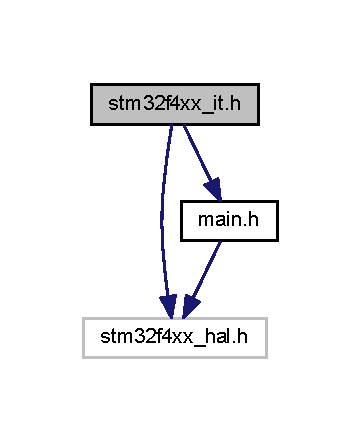
\includegraphics[width=173pt]{stm32f4xx__it_8h__incl}
\end{center}
\end{figure}
\subsection*{Functions}
\begin{DoxyCompactItemize}
\item 
void \mbox{\hyperlink{stm32f4xx__it_8h_a6ad7a5e3ee69cb6db6a6b9111ba898bc}{N\+M\+I\+\_\+\+Handler}} (void)
\item 
void \mbox{\hyperlink{stm32f4xx__it_8h_a2bffc10d5bd4106753b7c30e86903bea}{Hard\+Fault\+\_\+\+Handler}} (void)
\item 
void \mbox{\hyperlink{stm32f4xx__it_8h_a3150f74512510287a942624aa9b44cc5}{Mem\+Manage\+\_\+\+Handler}} (void)
\item 
void \mbox{\hyperlink{stm32f4xx__it_8h_a850cefb17a977292ae5eb4cafa9976c3}{Bus\+Fault\+\_\+\+Handler}} (void)
\item 
void \mbox{\hyperlink{stm32f4xx__it_8h_a1d98923de2ed6b7309b66f9ba2971647}{Usage\+Fault\+\_\+\+Handler}} (void)
\item 
void \mbox{\hyperlink{stm32f4xx__it_8h_a3e5ddb3df0d62f2dc357e64a3f04a6ce}{S\+V\+C\+\_\+\+Handler}} (void)
\item 
void \mbox{\hyperlink{stm32f4xx__it_8h_adbdfb05858cc36fc520974df37ec3cb0}{Debug\+Mon\+\_\+\+Handler}} (void)
\item 
void \mbox{\hyperlink{stm32f4xx__it_8h_a6303e1f258cbdc1f970ce579cc015623}{Pend\+S\+V\+\_\+\+Handler}} (void)
\item 
void \mbox{\hyperlink{stm32f4xx__it_8h_ab5e09814056d617c521549e542639b7e}{Sys\+Tick\+\_\+\+Handler}} (void)
\item 
void \mbox{\hyperlink{stm32f4xx__it_8h_ac201b60d58b0eba2ce0b55710eb3c4d0}{D\+M\+A1\+\_\+\+Stream5\+\_\+\+I\+R\+Q\+Handler}} (void)
\item 
void \mbox{\hyperlink{stm32f4xx__it_8h_aa28fd448462a6347589129f63bb0a388}{D\+M\+A1\+\_\+\+Stream6\+\_\+\+I\+R\+Q\+Handler}} (void)
\item 
void \mbox{\hyperlink{stm32f4xx__it_8h_a06406eadf297fa89a6eaf9586b227a69}{A\+D\+C\+\_\+\+I\+R\+Q\+Handler}} (void)
\item 
void \mbox{\hyperlink{stm32f4xx__it_8h_ac8e51d2183b5230cbd5481f8867adce9}{T\+I\+M3\+\_\+\+I\+R\+Q\+Handler}} (void)
\item 
void \mbox{\hyperlink{stm32f4xx__it_8h_a0ca6fd0e6f77921dd1123539857ba0a8}{U\+S\+A\+R\+T2\+\_\+\+I\+R\+Q\+Handler}} (void)
\item 
void \mbox{\hyperlink{stm32f4xx__it_8h_a5e66446caf21dd90191dc07a13ce2378}{T\+I\+M5\+\_\+\+I\+R\+Q\+Handler}} (void)
\end{DoxyCompactItemize}


\subsection{Detailed Description}
This file contains the headers of the interrupt handlers. 

C\+O\+P\+Y\+R\+I\+G\+H\+T(c) 2018 S\+T\+Microelectronics

Redistribution and use in source and binary forms, with or without modification, are permitted provided that the following conditions are met\+:
\begin{DoxyEnumerate}
\item Redistributions of source code must retain the above copyright notice, this list of conditions and the following disclaimer.
\item Redistributions in binary form must reproduce the above copyright notice, this list of conditions and the following disclaimer in the documentation and/or other materials provided with the distribution.
\item Neither the name of S\+T\+Microelectronics nor the names of its contributors may be used to endorse or promote products derived from this software without specific prior written permission.
\end{DoxyEnumerate}

T\+H\+IS S\+O\+F\+T\+W\+A\+RE IS P\+R\+O\+V\+I\+D\+ED BY T\+HE C\+O\+P\+Y\+R\+I\+G\+HT H\+O\+L\+D\+E\+RS A\+ND C\+O\+N\+T\+R\+I\+B\+U\+T\+O\+RS \char`\"{}\+A\+S I\+S\char`\"{} A\+ND A\+NY E\+X\+P\+R\+E\+SS OR I\+M\+P\+L\+I\+ED W\+A\+R\+R\+A\+N\+T\+I\+ES, I\+N\+C\+L\+U\+D\+I\+NG, B\+UT N\+OT L\+I\+M\+I\+T\+ED TO, T\+HE I\+M\+P\+L\+I\+ED W\+A\+R\+R\+A\+N\+T\+I\+ES OF M\+E\+R\+C\+H\+A\+N\+T\+A\+B\+I\+L\+I\+TY A\+ND F\+I\+T\+N\+E\+SS F\+OR A P\+A\+R\+T\+I\+C\+U\+L\+AR P\+U\+R\+P\+O\+SE A\+RE D\+I\+S\+C\+L\+A\+I\+M\+ED. IN NO E\+V\+E\+NT S\+H\+A\+LL T\+HE C\+O\+P\+Y\+R\+I\+G\+HT H\+O\+L\+D\+ER OR C\+O\+N\+T\+R\+I\+B\+U\+T\+O\+RS BE L\+I\+A\+B\+LE F\+OR A\+NY D\+I\+R\+E\+CT, I\+N\+D\+I\+R\+E\+CT, I\+N\+C\+I\+D\+E\+N\+T\+AL, S\+P\+E\+C\+I\+AL, E\+X\+E\+M\+P\+L\+A\+RY, OR C\+O\+N\+S\+E\+Q\+U\+E\+N\+T\+I\+AL D\+A\+M\+A\+G\+ES (I\+N\+C\+L\+U\+D\+I\+NG, B\+UT N\+OT L\+I\+M\+I\+T\+ED TO, P\+R\+O\+C\+U\+R\+E\+M\+E\+NT OF S\+U\+B\+S\+T\+I\+T\+U\+TE G\+O\+O\+DS OR S\+E\+R\+V\+I\+C\+ES; L\+O\+SS OF U\+SE, D\+A\+TA, OR P\+R\+O\+F\+I\+TS; OR B\+U\+S\+I\+N\+E\+SS I\+N\+T\+E\+R\+R\+U\+P\+T\+I\+ON) H\+O\+W\+E\+V\+ER C\+A\+U\+S\+ED A\+ND ON A\+NY T\+H\+E\+O\+RY OF L\+I\+A\+B\+I\+L\+I\+TY, W\+H\+E\+T\+H\+ER IN C\+O\+N\+T\+R\+A\+CT, S\+T\+R\+I\+CT L\+I\+A\+B\+I\+L\+I\+TY, OR T\+O\+RT (I\+N\+C\+L\+U\+D\+I\+NG N\+E\+G\+L\+I\+G\+E\+N\+CE OR O\+T\+H\+E\+R\+W\+I\+SE) A\+R\+I\+S\+I\+NG IN A\+NY W\+AY O\+UT OF T\+HE U\+SE OF T\+H\+IS S\+O\+F\+T\+W\+A\+RE, E\+V\+EN IF A\+D\+V\+I\+S\+ED OF T\+HE P\+O\+S\+S\+I\+B\+I\+L\+I\+TY OF S\+U\+CH D\+A\+M\+A\+GE. 

\subsection{Function Documentation}
\mbox{\Hypertarget{stm32f4xx__it_8h_a06406eadf297fa89a6eaf9586b227a69}\label{stm32f4xx__it_8h_a06406eadf297fa89a6eaf9586b227a69}} 
\index{stm32f4xx\+\_\+it.\+h@{stm32f4xx\+\_\+it.\+h}!A\+D\+C\+\_\+\+I\+R\+Q\+Handler@{A\+D\+C\+\_\+\+I\+R\+Q\+Handler}}
\index{A\+D\+C\+\_\+\+I\+R\+Q\+Handler@{A\+D\+C\+\_\+\+I\+R\+Q\+Handler}!stm32f4xx\+\_\+it.\+h@{stm32f4xx\+\_\+it.\+h}}
\subsubsection{\texorpdfstring{A\+D\+C\+\_\+\+I\+R\+Q\+Handler()}{ADC\_IRQHandler()}}
{\footnotesize\ttfamily void A\+D\+C\+\_\+\+I\+R\+Q\+Handler (\begin{DoxyParamCaption}\item[{void}]{ }\end{DoxyParamCaption})}

\mbox{\Hypertarget{stm32f4xx__it_8h_a850cefb17a977292ae5eb4cafa9976c3}\label{stm32f4xx__it_8h_a850cefb17a977292ae5eb4cafa9976c3}} 
\index{stm32f4xx\+\_\+it.\+h@{stm32f4xx\+\_\+it.\+h}!Bus\+Fault\+\_\+\+Handler@{Bus\+Fault\+\_\+\+Handler}}
\index{Bus\+Fault\+\_\+\+Handler@{Bus\+Fault\+\_\+\+Handler}!stm32f4xx\+\_\+it.\+h@{stm32f4xx\+\_\+it.\+h}}
\subsubsection{\texorpdfstring{Bus\+Fault\+\_\+\+Handler()}{BusFault\_Handler()}}
{\footnotesize\ttfamily void Bus\+Fault\+\_\+\+Handler (\begin{DoxyParamCaption}\item[{void}]{ }\end{DoxyParamCaption})}

\mbox{\Hypertarget{stm32f4xx__it_8h_adbdfb05858cc36fc520974df37ec3cb0}\label{stm32f4xx__it_8h_adbdfb05858cc36fc520974df37ec3cb0}} 
\index{stm32f4xx\+\_\+it.\+h@{stm32f4xx\+\_\+it.\+h}!Debug\+Mon\+\_\+\+Handler@{Debug\+Mon\+\_\+\+Handler}}
\index{Debug\+Mon\+\_\+\+Handler@{Debug\+Mon\+\_\+\+Handler}!stm32f4xx\+\_\+it.\+h@{stm32f4xx\+\_\+it.\+h}}
\subsubsection{\texorpdfstring{Debug\+Mon\+\_\+\+Handler()}{DebugMon\_Handler()}}
{\footnotesize\ttfamily void Debug\+Mon\+\_\+\+Handler (\begin{DoxyParamCaption}\item[{void}]{ }\end{DoxyParamCaption})}

\mbox{\Hypertarget{stm32f4xx__it_8h_ac201b60d58b0eba2ce0b55710eb3c4d0}\label{stm32f4xx__it_8h_ac201b60d58b0eba2ce0b55710eb3c4d0}} 
\index{stm32f4xx\+\_\+it.\+h@{stm32f4xx\+\_\+it.\+h}!D\+M\+A1\+\_\+\+Stream5\+\_\+\+I\+R\+Q\+Handler@{D\+M\+A1\+\_\+\+Stream5\+\_\+\+I\+R\+Q\+Handler}}
\index{D\+M\+A1\+\_\+\+Stream5\+\_\+\+I\+R\+Q\+Handler@{D\+M\+A1\+\_\+\+Stream5\+\_\+\+I\+R\+Q\+Handler}!stm32f4xx\+\_\+it.\+h@{stm32f4xx\+\_\+it.\+h}}
\subsubsection{\texorpdfstring{D\+M\+A1\+\_\+\+Stream5\+\_\+\+I\+R\+Q\+Handler()}{DMA1\_Stream5\_IRQHandler()}}
{\footnotesize\ttfamily void D\+M\+A1\+\_\+\+Stream5\+\_\+\+I\+R\+Q\+Handler (\begin{DoxyParamCaption}\item[{void}]{ }\end{DoxyParamCaption})}

\mbox{\Hypertarget{stm32f4xx__it_8h_aa28fd448462a6347589129f63bb0a388}\label{stm32f4xx__it_8h_aa28fd448462a6347589129f63bb0a388}} 
\index{stm32f4xx\+\_\+it.\+h@{stm32f4xx\+\_\+it.\+h}!D\+M\+A1\+\_\+\+Stream6\+\_\+\+I\+R\+Q\+Handler@{D\+M\+A1\+\_\+\+Stream6\+\_\+\+I\+R\+Q\+Handler}}
\index{D\+M\+A1\+\_\+\+Stream6\+\_\+\+I\+R\+Q\+Handler@{D\+M\+A1\+\_\+\+Stream6\+\_\+\+I\+R\+Q\+Handler}!stm32f4xx\+\_\+it.\+h@{stm32f4xx\+\_\+it.\+h}}
\subsubsection{\texorpdfstring{D\+M\+A1\+\_\+\+Stream6\+\_\+\+I\+R\+Q\+Handler()}{DMA1\_Stream6\_IRQHandler()}}
{\footnotesize\ttfamily void D\+M\+A1\+\_\+\+Stream6\+\_\+\+I\+R\+Q\+Handler (\begin{DoxyParamCaption}\item[{void}]{ }\end{DoxyParamCaption})}

\mbox{\Hypertarget{stm32f4xx__it_8h_a2bffc10d5bd4106753b7c30e86903bea}\label{stm32f4xx__it_8h_a2bffc10d5bd4106753b7c30e86903bea}} 
\index{stm32f4xx\+\_\+it.\+h@{stm32f4xx\+\_\+it.\+h}!Hard\+Fault\+\_\+\+Handler@{Hard\+Fault\+\_\+\+Handler}}
\index{Hard\+Fault\+\_\+\+Handler@{Hard\+Fault\+\_\+\+Handler}!stm32f4xx\+\_\+it.\+h@{stm32f4xx\+\_\+it.\+h}}
\subsubsection{\texorpdfstring{Hard\+Fault\+\_\+\+Handler()}{HardFault\_Handler()}}
{\footnotesize\ttfamily void Hard\+Fault\+\_\+\+Handler (\begin{DoxyParamCaption}\item[{void}]{ }\end{DoxyParamCaption})}

\mbox{\Hypertarget{stm32f4xx__it_8h_a3150f74512510287a942624aa9b44cc5}\label{stm32f4xx__it_8h_a3150f74512510287a942624aa9b44cc5}} 
\index{stm32f4xx\+\_\+it.\+h@{stm32f4xx\+\_\+it.\+h}!Mem\+Manage\+\_\+\+Handler@{Mem\+Manage\+\_\+\+Handler}}
\index{Mem\+Manage\+\_\+\+Handler@{Mem\+Manage\+\_\+\+Handler}!stm32f4xx\+\_\+it.\+h@{stm32f4xx\+\_\+it.\+h}}
\subsubsection{\texorpdfstring{Mem\+Manage\+\_\+\+Handler()}{MemManage\_Handler()}}
{\footnotesize\ttfamily void Mem\+Manage\+\_\+\+Handler (\begin{DoxyParamCaption}\item[{void}]{ }\end{DoxyParamCaption})}

\mbox{\Hypertarget{stm32f4xx__it_8h_a6ad7a5e3ee69cb6db6a6b9111ba898bc}\label{stm32f4xx__it_8h_a6ad7a5e3ee69cb6db6a6b9111ba898bc}} 
\index{stm32f4xx\+\_\+it.\+h@{stm32f4xx\+\_\+it.\+h}!N\+M\+I\+\_\+\+Handler@{N\+M\+I\+\_\+\+Handler}}
\index{N\+M\+I\+\_\+\+Handler@{N\+M\+I\+\_\+\+Handler}!stm32f4xx\+\_\+it.\+h@{stm32f4xx\+\_\+it.\+h}}
\subsubsection{\texorpdfstring{N\+M\+I\+\_\+\+Handler()}{NMI\_Handler()}}
{\footnotesize\ttfamily void N\+M\+I\+\_\+\+Handler (\begin{DoxyParamCaption}\item[{void}]{ }\end{DoxyParamCaption})}

\mbox{\Hypertarget{stm32f4xx__it_8h_a6303e1f258cbdc1f970ce579cc015623}\label{stm32f4xx__it_8h_a6303e1f258cbdc1f970ce579cc015623}} 
\index{stm32f4xx\+\_\+it.\+h@{stm32f4xx\+\_\+it.\+h}!Pend\+S\+V\+\_\+\+Handler@{Pend\+S\+V\+\_\+\+Handler}}
\index{Pend\+S\+V\+\_\+\+Handler@{Pend\+S\+V\+\_\+\+Handler}!stm32f4xx\+\_\+it.\+h@{stm32f4xx\+\_\+it.\+h}}
\subsubsection{\texorpdfstring{Pend\+S\+V\+\_\+\+Handler()}{PendSV\_Handler()}}
{\footnotesize\ttfamily void Pend\+S\+V\+\_\+\+Handler (\begin{DoxyParamCaption}\item[{void}]{ }\end{DoxyParamCaption})}

\mbox{\Hypertarget{stm32f4xx__it_8h_a3e5ddb3df0d62f2dc357e64a3f04a6ce}\label{stm32f4xx__it_8h_a3e5ddb3df0d62f2dc357e64a3f04a6ce}} 
\index{stm32f4xx\+\_\+it.\+h@{stm32f4xx\+\_\+it.\+h}!S\+V\+C\+\_\+\+Handler@{S\+V\+C\+\_\+\+Handler}}
\index{S\+V\+C\+\_\+\+Handler@{S\+V\+C\+\_\+\+Handler}!stm32f4xx\+\_\+it.\+h@{stm32f4xx\+\_\+it.\+h}}
\subsubsection{\texorpdfstring{S\+V\+C\+\_\+\+Handler()}{SVC\_Handler()}}
{\footnotesize\ttfamily void S\+V\+C\+\_\+\+Handler (\begin{DoxyParamCaption}\item[{void}]{ }\end{DoxyParamCaption})}

\mbox{\Hypertarget{stm32f4xx__it_8h_ab5e09814056d617c521549e542639b7e}\label{stm32f4xx__it_8h_ab5e09814056d617c521549e542639b7e}} 
\index{stm32f4xx\+\_\+it.\+h@{stm32f4xx\+\_\+it.\+h}!Sys\+Tick\+\_\+\+Handler@{Sys\+Tick\+\_\+\+Handler}}
\index{Sys\+Tick\+\_\+\+Handler@{Sys\+Tick\+\_\+\+Handler}!stm32f4xx\+\_\+it.\+h@{stm32f4xx\+\_\+it.\+h}}
\subsubsection{\texorpdfstring{Sys\+Tick\+\_\+\+Handler()}{SysTick\_Handler()}}
{\footnotesize\ttfamily void Sys\+Tick\+\_\+\+Handler (\begin{DoxyParamCaption}\item[{void}]{ }\end{DoxyParamCaption})}

\mbox{\Hypertarget{stm32f4xx__it_8h_ac8e51d2183b5230cbd5481f8867adce9}\label{stm32f4xx__it_8h_ac8e51d2183b5230cbd5481f8867adce9}} 
\index{stm32f4xx\+\_\+it.\+h@{stm32f4xx\+\_\+it.\+h}!T\+I\+M3\+\_\+\+I\+R\+Q\+Handler@{T\+I\+M3\+\_\+\+I\+R\+Q\+Handler}}
\index{T\+I\+M3\+\_\+\+I\+R\+Q\+Handler@{T\+I\+M3\+\_\+\+I\+R\+Q\+Handler}!stm32f4xx\+\_\+it.\+h@{stm32f4xx\+\_\+it.\+h}}
\subsubsection{\texorpdfstring{T\+I\+M3\+\_\+\+I\+R\+Q\+Handler()}{TIM3\_IRQHandler()}}
{\footnotesize\ttfamily void T\+I\+M3\+\_\+\+I\+R\+Q\+Handler (\begin{DoxyParamCaption}\item[{void}]{ }\end{DoxyParamCaption})}

\mbox{\Hypertarget{stm32f4xx__it_8h_a5e66446caf21dd90191dc07a13ce2378}\label{stm32f4xx__it_8h_a5e66446caf21dd90191dc07a13ce2378}} 
\index{stm32f4xx\+\_\+it.\+h@{stm32f4xx\+\_\+it.\+h}!T\+I\+M5\+\_\+\+I\+R\+Q\+Handler@{T\+I\+M5\+\_\+\+I\+R\+Q\+Handler}}
\index{T\+I\+M5\+\_\+\+I\+R\+Q\+Handler@{T\+I\+M5\+\_\+\+I\+R\+Q\+Handler}!stm32f4xx\+\_\+it.\+h@{stm32f4xx\+\_\+it.\+h}}
\subsubsection{\texorpdfstring{T\+I\+M5\+\_\+\+I\+R\+Q\+Handler()}{TIM5\_IRQHandler()}}
{\footnotesize\ttfamily void T\+I\+M5\+\_\+\+I\+R\+Q\+Handler (\begin{DoxyParamCaption}\item[{void}]{ }\end{DoxyParamCaption})}

\mbox{\Hypertarget{stm32f4xx__it_8h_a1d98923de2ed6b7309b66f9ba2971647}\label{stm32f4xx__it_8h_a1d98923de2ed6b7309b66f9ba2971647}} 
\index{stm32f4xx\+\_\+it.\+h@{stm32f4xx\+\_\+it.\+h}!Usage\+Fault\+\_\+\+Handler@{Usage\+Fault\+\_\+\+Handler}}
\index{Usage\+Fault\+\_\+\+Handler@{Usage\+Fault\+\_\+\+Handler}!stm32f4xx\+\_\+it.\+h@{stm32f4xx\+\_\+it.\+h}}
\subsubsection{\texorpdfstring{Usage\+Fault\+\_\+\+Handler()}{UsageFault\_Handler()}}
{\footnotesize\ttfamily void Usage\+Fault\+\_\+\+Handler (\begin{DoxyParamCaption}\item[{void}]{ }\end{DoxyParamCaption})}

\mbox{\Hypertarget{stm32f4xx__it_8h_a0ca6fd0e6f77921dd1123539857ba0a8}\label{stm32f4xx__it_8h_a0ca6fd0e6f77921dd1123539857ba0a8}} 
\index{stm32f4xx\+\_\+it.\+h@{stm32f4xx\+\_\+it.\+h}!U\+S\+A\+R\+T2\+\_\+\+I\+R\+Q\+Handler@{U\+S\+A\+R\+T2\+\_\+\+I\+R\+Q\+Handler}}
\index{U\+S\+A\+R\+T2\+\_\+\+I\+R\+Q\+Handler@{U\+S\+A\+R\+T2\+\_\+\+I\+R\+Q\+Handler}!stm32f4xx\+\_\+it.\+h@{stm32f4xx\+\_\+it.\+h}}
\subsubsection{\texorpdfstring{U\+S\+A\+R\+T2\+\_\+\+I\+R\+Q\+Handler()}{USART2\_IRQHandler()}}
{\footnotesize\ttfamily void U\+S\+A\+R\+T2\+\_\+\+I\+R\+Q\+Handler (\begin{DoxyParamCaption}\item[{void}]{ }\end{DoxyParamCaption})}


\hypertarget{tim_8h}{}\section{tim.\+h File Reference}
\label{tim_8h}\index{tim.\+h@{tim.\+h}}
{\ttfamily \#include \char`\"{}stm32f4xx\+\_\+hal.\+h\char`\"{}}\newline
{\ttfamily \#include \char`\"{}main.\+h\char`\"{}}\newline
Include dependency graph for tim.\+h\+:\nopagebreak
\begin{figure}[H]
\begin{center}
\leavevmode
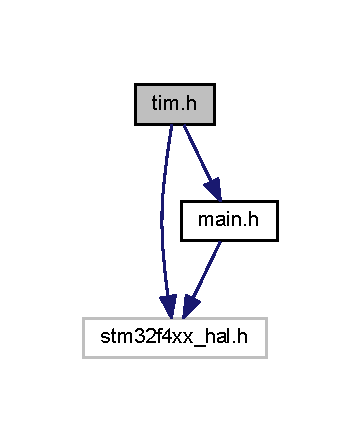
\includegraphics[width=173pt]{tim_8h__incl}
\end{center}
\end{figure}
This graph shows which files directly or indirectly include this file\+:\nopagebreak
\begin{figure}[H]
\begin{center}
\leavevmode
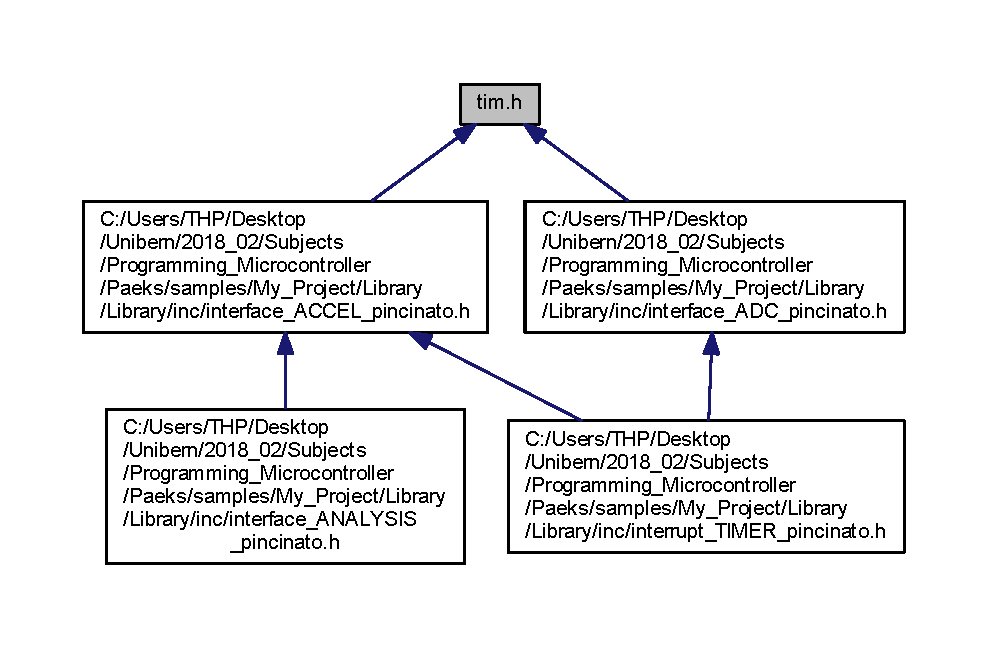
\includegraphics[width=350pt]{tim_8h__dep__incl}
\end{center}
\end{figure}
\subsection*{Functions}
\begin{DoxyCompactItemize}
\item 
void \mbox{\hyperlink{tim_8h_a47642651029b93e3f9c9edad46bd27b4}{\+\_\+\+Error\+\_\+\+Handler}} (char $\ast$, int)
\item 
void \mbox{\hyperlink{tim_8h_a7912f2916786a2c33cb6fb8259ade58c}{M\+X\+\_\+\+T\+I\+M3\+\_\+\+Init}} (void)
\item 
void \mbox{\hyperlink{tim_8h_a5ee937d52485d5cda27896e3842a7ca1}{M\+X\+\_\+\+T\+I\+M5\+\_\+\+Init}} (void)
\item 
void \mbox{\hyperlink{tim_8h_ae70bce6c39d0b570a7523b86738cec4b}{H\+A\+L\+\_\+\+T\+I\+M\+\_\+\+Msp\+Post\+Init}} (T\+I\+M\+\_\+\+Handle\+Type\+Def $\ast$htim)
\end{DoxyCompactItemize}
\subsection*{Variables}
\begin{DoxyCompactItemize}
\item 
T\+I\+M\+\_\+\+Handle\+Type\+Def \mbox{\hyperlink{tim_8h_aac3d2c59ee0e3bbae1b99529a154eb62}{htim3}}
\item 
T\+I\+M\+\_\+\+Handle\+Type\+Def \mbox{\hyperlink{tim_8h_acefaeaaa3856ddddae7083b2d220fe4b}{htim5}}
\end{DoxyCompactItemize}


\subsection{Function Documentation}
\mbox{\Hypertarget{tim_8h_a47642651029b93e3f9c9edad46bd27b4}\label{tim_8h_a47642651029b93e3f9c9edad46bd27b4}} 
\index{tim.\+h@{tim.\+h}!\+\_\+\+Error\+\_\+\+Handler@{\+\_\+\+Error\+\_\+\+Handler}}
\index{\+\_\+\+Error\+\_\+\+Handler@{\+\_\+\+Error\+\_\+\+Handler}!tim.\+h@{tim.\+h}}
\subsubsection{\texorpdfstring{\+\_\+\+Error\+\_\+\+Handler()}{\_Error\_Handler()}}
{\footnotesize\ttfamily void \+\_\+\+Error\+\_\+\+Handler (\begin{DoxyParamCaption}\item[{char $\ast$}]{,  }\item[{int}]{ }\end{DoxyParamCaption})}

\mbox{\Hypertarget{tim_8h_ae70bce6c39d0b570a7523b86738cec4b}\label{tim_8h_ae70bce6c39d0b570a7523b86738cec4b}} 
\index{tim.\+h@{tim.\+h}!H\+A\+L\+\_\+\+T\+I\+M\+\_\+\+Msp\+Post\+Init@{H\+A\+L\+\_\+\+T\+I\+M\+\_\+\+Msp\+Post\+Init}}
\index{H\+A\+L\+\_\+\+T\+I\+M\+\_\+\+Msp\+Post\+Init@{H\+A\+L\+\_\+\+T\+I\+M\+\_\+\+Msp\+Post\+Init}!tim.\+h@{tim.\+h}}
\subsubsection{\texorpdfstring{H\+A\+L\+\_\+\+T\+I\+M\+\_\+\+Msp\+Post\+Init()}{HAL\_TIM\_MspPostInit()}}
{\footnotesize\ttfamily void H\+A\+L\+\_\+\+T\+I\+M\+\_\+\+Msp\+Post\+Init (\begin{DoxyParamCaption}\item[{T\+I\+M\+\_\+\+Handle\+Type\+Def $\ast$}]{htim }\end{DoxyParamCaption})}

\mbox{\Hypertarget{tim_8h_a7912f2916786a2c33cb6fb8259ade58c}\label{tim_8h_a7912f2916786a2c33cb6fb8259ade58c}} 
\index{tim.\+h@{tim.\+h}!M\+X\+\_\+\+T\+I\+M3\+\_\+\+Init@{M\+X\+\_\+\+T\+I\+M3\+\_\+\+Init}}
\index{M\+X\+\_\+\+T\+I\+M3\+\_\+\+Init@{M\+X\+\_\+\+T\+I\+M3\+\_\+\+Init}!tim.\+h@{tim.\+h}}
\subsubsection{\texorpdfstring{M\+X\+\_\+\+T\+I\+M3\+\_\+\+Init()}{MX\_TIM3\_Init()}}
{\footnotesize\ttfamily void M\+X\+\_\+\+T\+I\+M3\+\_\+\+Init (\begin{DoxyParamCaption}\item[{void}]{ }\end{DoxyParamCaption})}

\mbox{\Hypertarget{tim_8h_a5ee937d52485d5cda27896e3842a7ca1}\label{tim_8h_a5ee937d52485d5cda27896e3842a7ca1}} 
\index{tim.\+h@{tim.\+h}!M\+X\+\_\+\+T\+I\+M5\+\_\+\+Init@{M\+X\+\_\+\+T\+I\+M5\+\_\+\+Init}}
\index{M\+X\+\_\+\+T\+I\+M5\+\_\+\+Init@{M\+X\+\_\+\+T\+I\+M5\+\_\+\+Init}!tim.\+h@{tim.\+h}}
\subsubsection{\texorpdfstring{M\+X\+\_\+\+T\+I\+M5\+\_\+\+Init()}{MX\_TIM5\_Init()}}
{\footnotesize\ttfamily void M\+X\+\_\+\+T\+I\+M5\+\_\+\+Init (\begin{DoxyParamCaption}\item[{void}]{ }\end{DoxyParamCaption})}



\subsection{Variable Documentation}
\mbox{\Hypertarget{tim_8h_aac3d2c59ee0e3bbae1b99529a154eb62}\label{tim_8h_aac3d2c59ee0e3bbae1b99529a154eb62}} 
\index{tim.\+h@{tim.\+h}!htim3@{htim3}}
\index{htim3@{htim3}!tim.\+h@{tim.\+h}}
\subsubsection{\texorpdfstring{htim3}{htim3}}
{\footnotesize\ttfamily T\+I\+M\+\_\+\+Handle\+Type\+Def htim3}

File Name \+: \mbox{\hyperlink{tim_8h}{T\+I\+M.\+h}} Description \+: This file provides code for the configuration of the T\+IM instances.

This notice applies to any and all portions of this file that are not between comment pairs U\+S\+ER C\+O\+DE B\+E\+G\+IN and U\+S\+ER C\+O\+DE E\+ND. Other portions of this file, whether inserted by the user or by software development tools are owned by their respective copyright owners.

Copyright (c) 2018 S\+T\+Microelectronics International N.\+V. All rights reserved.

Redistribution and use in source and binary forms, with or without modification, are permitted, provided that the following conditions are met\+:


\begin{DoxyEnumerate}
\item Redistribution of source code must retain the above copyright notice, this list of conditions and the following disclaimer.
\item Redistributions in binary form must reproduce the above copyright notice, this list of conditions and the following disclaimer in the documentation and/or other materials provided with the distribution.
\item Neither the name of S\+T\+Microelectronics nor the names of other contributors to this software may be used to endorse or promote products derived from this software without specific written permission.
\item This software, including modifications and/or derivative works of this software, must execute solely and exclusively on microcontroller or microprocessor devices manufactured by or for S\+T\+Microelectronics.
\item Redistribution and use of this software other than as permitted under this license is void and will automatically terminate your rights under this license.
\end{DoxyEnumerate}

T\+H\+IS S\+O\+F\+T\+W\+A\+RE IS P\+R\+O\+V\+I\+D\+ED BY S\+T\+M\+I\+C\+R\+O\+E\+L\+E\+C\+T\+R\+O\+N\+I\+CS A\+ND C\+O\+N\+T\+R\+I\+B\+U\+T\+O\+RS \char`\"{}\+A\+S I\+S\char`\"{} A\+ND A\+NY E\+X\+P\+R\+E\+SS, I\+M\+P\+L\+I\+ED OR S\+T\+A\+T\+U\+T\+O\+RY W\+A\+R\+R\+A\+N\+T\+I\+ES, I\+N\+C\+L\+U\+D\+I\+NG, B\+UT N\+OT L\+I\+M\+I\+T\+ED TO, T\+HE I\+M\+P\+L\+I\+ED W\+A\+R\+R\+A\+N\+T\+I\+ES OF M\+E\+R\+C\+H\+A\+N\+T\+A\+B\+I\+L\+I\+TY, F\+I\+T\+N\+E\+SS F\+OR A P\+A\+R\+T\+I\+C\+U\+L\+AR P\+U\+R\+P\+O\+SE A\+ND N\+O\+N-\/\+I\+N\+F\+R\+I\+N\+G\+E\+M\+E\+NT OF T\+H\+I\+RD P\+A\+R\+TY I\+N\+T\+E\+L\+L\+E\+C\+T\+U\+AL P\+R\+O\+P\+E\+R\+TY R\+I\+G\+H\+TS A\+RE D\+I\+S\+C\+L\+A\+I\+M\+ED TO T\+HE F\+U\+L\+L\+E\+ST E\+X\+T\+E\+NT P\+E\+R\+M\+I\+T\+T\+ED BY L\+AW. IN NO E\+V\+E\+NT S\+H\+A\+LL S\+T\+M\+I\+C\+R\+O\+E\+L\+E\+C\+T\+R\+O\+N\+I\+CS OR C\+O\+N\+T\+R\+I\+B\+U\+T\+O\+RS BE L\+I\+A\+B\+LE F\+OR A\+NY D\+I\+R\+E\+CT, I\+N\+D\+I\+R\+E\+CT, I\+N\+C\+I\+D\+E\+N\+T\+AL, S\+P\+E\+C\+I\+AL, E\+X\+E\+M\+P\+L\+A\+RY, OR C\+O\+N\+S\+E\+Q\+U\+E\+N\+T\+I\+AL D\+A\+M\+A\+G\+ES (I\+N\+C\+L\+U\+D\+I\+NG, B\+UT N\+OT L\+I\+M\+I\+T\+ED TO, P\+R\+O\+C\+U\+R\+E\+M\+E\+NT OF S\+U\+B\+S\+T\+I\+T\+U\+TE G\+O\+O\+DS OR S\+E\+R\+V\+I\+C\+ES; L\+O\+SS OF U\+SE, D\+A\+TA, OR P\+R\+O\+F\+I\+TS; OR B\+U\+S\+I\+N\+E\+SS I\+N\+T\+E\+R\+R\+U\+P\+T\+I\+ON) H\+O\+W\+E\+V\+ER C\+A\+U\+S\+ED A\+ND ON A\+NY T\+H\+E\+O\+RY OF L\+I\+A\+B\+I\+L\+I\+TY, W\+H\+E\+T\+H\+ER IN C\+O\+N\+T\+R\+A\+CT, S\+T\+R\+I\+CT L\+I\+A\+B\+I\+L\+I\+TY, OR T\+O\+RT (I\+N\+C\+L\+U\+D\+I\+NG N\+E\+G\+L\+I\+G\+E\+N\+CE OR O\+T\+H\+E\+R\+W\+I\+SE) A\+R\+I\+S\+I\+NG IN A\+NY W\+AY O\+UT OF T\+HE U\+SE OF T\+H\+IS S\+O\+F\+T\+W\+A\+RE, E\+V\+EN IF A\+D\+V\+I\+S\+ED OF T\+HE P\+O\+S\+S\+I\+B\+I\+L\+I\+TY OF S\+U\+CH D\+A\+M\+A\+GE. \mbox{\Hypertarget{tim_8h_acefaeaaa3856ddddae7083b2d220fe4b}\label{tim_8h_acefaeaaa3856ddddae7083b2d220fe4b}} 
\index{tim.\+h@{tim.\+h}!htim5@{htim5}}
\index{htim5@{htim5}!tim.\+h@{tim.\+h}}
\subsubsection{\texorpdfstring{htim5}{htim5}}
{\footnotesize\ttfamily T\+I\+M\+\_\+\+Handle\+Type\+Def htim5}


\hypertarget{usart_8h}{}\section{Inc/usart.h File Reference}
\label{usart_8h}\index{Inc/usart.\+h@{Inc/usart.\+h}}
{\ttfamily \#include \char`\"{}stm32f4xx\+\_\+hal.\+h\char`\"{}}\newline
{\ttfamily \#include \char`\"{}main.\+h\char`\"{}}\newline
Include dependency graph for usart.\+h\+:\nopagebreak
\begin{figure}[H]
\begin{center}
\leavevmode
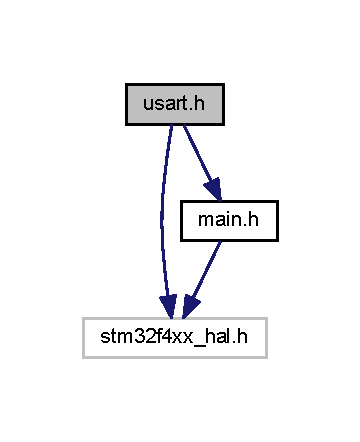
\includegraphics[width=173pt]{usart_8h__incl}
\end{center}
\end{figure}
This graph shows which files directly or indirectly include this file\+:\nopagebreak
\begin{figure}[H]
\begin{center}
\leavevmode
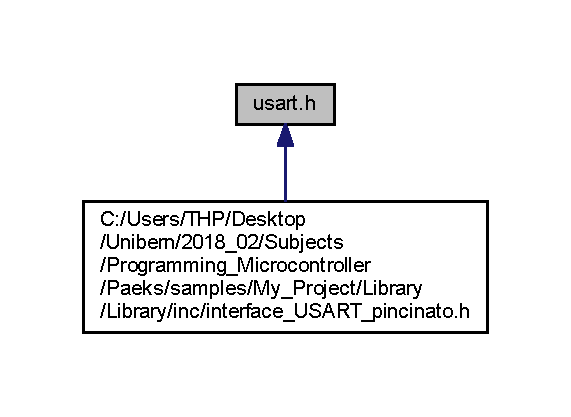
\includegraphics[width=350pt]{usart_8h__dep__incl}
\end{center}
\end{figure}
\subsection*{Functions}
\begin{DoxyCompactItemize}
\item 
void \mbox{\hyperlink{usart_8h_a47642651029b93e3f9c9edad46bd27b4}{\+\_\+\+Error\+\_\+\+Handler}} (char $\ast$, int)
\begin{DoxyCompactList}\small\item\em This function is executed in case of error occurrence. \end{DoxyCompactList}\item 
void \mbox{\hyperlink{usart_8h_a052088fe5bb3f807a4b2502e664fd4fd}{M\+X\+\_\+\+U\+S\+A\+R\+T2\+\_\+\+U\+A\+R\+T\+\_\+\+Init}} (void)
\end{DoxyCompactItemize}
\subsection*{Variables}
\begin{DoxyCompactItemize}
\item 
U\+A\+R\+T\+\_\+\+Handle\+Type\+Def \mbox{\hyperlink{usart_8h_aa9479c261d65eecedd3d9582f7f0f89c}{huart2}}
\end{DoxyCompactItemize}


\subsection{Function Documentation}
\mbox{\Hypertarget{usart_8h_a47642651029b93e3f9c9edad46bd27b4}\label{usart_8h_a47642651029b93e3f9c9edad46bd27b4}} 
\index{usart.\+h@{usart.\+h}!\+\_\+\+Error\+\_\+\+Handler@{\+\_\+\+Error\+\_\+\+Handler}}
\index{\+\_\+\+Error\+\_\+\+Handler@{\+\_\+\+Error\+\_\+\+Handler}!usart.\+h@{usart.\+h}}
\subsubsection{\texorpdfstring{\+\_\+\+Error\+\_\+\+Handler()}{\_Error\_Handler()}}
{\footnotesize\ttfamily void \+\_\+\+Error\+\_\+\+Handler (\begin{DoxyParamCaption}\item[{char $\ast$}]{file,  }\item[{int}]{line }\end{DoxyParamCaption})}



This function is executed in case of error occurrence. 


\begin{DoxyParams}{Parameters}
{\em file} & The file name as string. \\
\hline
{\em line} & The line in file as a number. \\
\hline
\end{DoxyParams}

\begin{DoxyRetVals}{Return values}
{\em None} & \\
\hline
\end{DoxyRetVals}


Definition at line 430 of file main.\+c.

\mbox{\Hypertarget{usart_8h_a052088fe5bb3f807a4b2502e664fd4fd}\label{usart_8h_a052088fe5bb3f807a4b2502e664fd4fd}} 
\index{usart.\+h@{usart.\+h}!M\+X\+\_\+\+U\+S\+A\+R\+T2\+\_\+\+U\+A\+R\+T\+\_\+\+Init@{M\+X\+\_\+\+U\+S\+A\+R\+T2\+\_\+\+U\+A\+R\+T\+\_\+\+Init}}
\index{M\+X\+\_\+\+U\+S\+A\+R\+T2\+\_\+\+U\+A\+R\+T\+\_\+\+Init@{M\+X\+\_\+\+U\+S\+A\+R\+T2\+\_\+\+U\+A\+R\+T\+\_\+\+Init}!usart.\+h@{usart.\+h}}
\subsubsection{\texorpdfstring{M\+X\+\_\+\+U\+S\+A\+R\+T2\+\_\+\+U\+A\+R\+T\+\_\+\+Init()}{MX\_USART2\_UART\_Init()}}
{\footnotesize\ttfamily void M\+X\+\_\+\+U\+S\+A\+R\+T2\+\_\+\+U\+A\+R\+T\+\_\+\+Init (\begin{DoxyParamCaption}\item[{void}]{ }\end{DoxyParamCaption})}



Definition at line 66 of file usart.\+c.

Here is the call graph for this function\+:\nopagebreak
\begin{figure}[H]
\begin{center}
\leavevmode
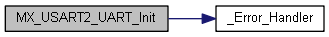
\includegraphics[width=319pt]{usart_8h_a052088fe5bb3f807a4b2502e664fd4fd_cgraph}
\end{center}
\end{figure}
Here is the caller graph for this function\+:\nopagebreak
\begin{figure}[H]
\begin{center}
\leavevmode
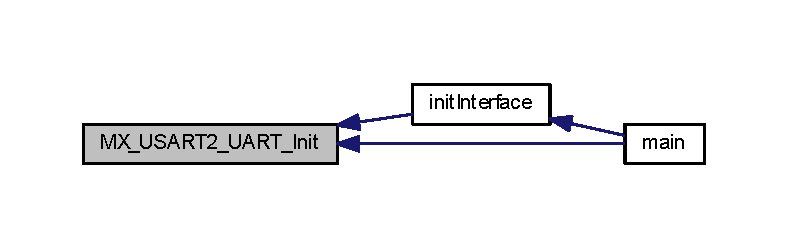
\includegraphics[width=350pt]{usart_8h_a052088fe5bb3f807a4b2502e664fd4fd_icgraph}
\end{center}
\end{figure}


\subsection{Variable Documentation}
\mbox{\Hypertarget{usart_8h_aa9479c261d65eecedd3d9582f7f0f89c}\label{usart_8h_aa9479c261d65eecedd3d9582f7f0f89c}} 
\index{usart.\+h@{usart.\+h}!huart2@{huart2}}
\index{huart2@{huart2}!usart.\+h@{usart.\+h}}
\subsubsection{\texorpdfstring{huart2}{huart2}}
{\footnotesize\ttfamily U\+A\+R\+T\+\_\+\+Handle\+Type\+Def huart2}

File Name \+: \mbox{\hyperlink{usart_8h}{U\+S\+A\+R\+T.\+h}} Description \+: This file provides code for the configuration of the U\+S\+A\+RT instances.

This notice applies to any and all portions of this file that are not between comment pairs U\+S\+ER C\+O\+DE B\+E\+G\+IN and U\+S\+ER C\+O\+DE E\+ND. Other portions of this file, whether inserted by the user or by software development tools are owned by their respective copyright owners.

Copyright (c) 2018 S\+T\+Microelectronics International N.\+V. All rights reserved.

Redistribution and use in source and binary forms, with or without modification, are permitted, provided that the following conditions are met\+:


\begin{DoxyEnumerate}
\item Redistribution of source code must retain the above copyright notice, this list of conditions and the following disclaimer.
\item Redistributions in binary form must reproduce the above copyright notice, this list of conditions and the following disclaimer in the documentation and/or other materials provided with the distribution.
\item Neither the name of S\+T\+Microelectronics nor the names of other contributors to this software may be used to endorse or promote products derived from this software without specific written permission.
\item This software, including modifications and/or derivative works of this software, must execute solely and exclusively on microcontroller or microprocessor devices manufactured by or for S\+T\+Microelectronics.
\item Redistribution and use of this software other than as permitted under this license is void and will automatically terminate your rights under this license.
\end{DoxyEnumerate}

T\+H\+IS S\+O\+F\+T\+W\+A\+RE IS P\+R\+O\+V\+I\+D\+ED BY S\+T\+M\+I\+C\+R\+O\+E\+L\+E\+C\+T\+R\+O\+N\+I\+CS A\+ND C\+O\+N\+T\+R\+I\+B\+U\+T\+O\+RS \char`\"{}\+A\+S I\+S\char`\"{} A\+ND A\+NY E\+X\+P\+R\+E\+SS, I\+M\+P\+L\+I\+ED OR S\+T\+A\+T\+U\+T\+O\+RY W\+A\+R\+R\+A\+N\+T\+I\+ES, I\+N\+C\+L\+U\+D\+I\+NG, B\+UT N\+OT L\+I\+M\+I\+T\+ED TO, T\+HE I\+M\+P\+L\+I\+ED W\+A\+R\+R\+A\+N\+T\+I\+ES OF M\+E\+R\+C\+H\+A\+N\+T\+A\+B\+I\+L\+I\+TY, F\+I\+T\+N\+E\+SS F\+OR A P\+A\+R\+T\+I\+C\+U\+L\+AR P\+U\+R\+P\+O\+SE A\+ND N\+O\+N-\/\+I\+N\+F\+R\+I\+N\+G\+E\+M\+E\+NT OF T\+H\+I\+RD P\+A\+R\+TY I\+N\+T\+E\+L\+L\+E\+C\+T\+U\+AL P\+R\+O\+P\+E\+R\+TY R\+I\+G\+H\+TS A\+RE D\+I\+S\+C\+L\+A\+I\+M\+ED TO T\+HE F\+U\+L\+L\+E\+ST E\+X\+T\+E\+NT P\+E\+R\+M\+I\+T\+T\+ED BY L\+AW. IN NO E\+V\+E\+NT S\+H\+A\+LL S\+T\+M\+I\+C\+R\+O\+E\+L\+E\+C\+T\+R\+O\+N\+I\+CS OR C\+O\+N\+T\+R\+I\+B\+U\+T\+O\+RS BE L\+I\+A\+B\+LE F\+OR A\+NY D\+I\+R\+E\+CT, I\+N\+D\+I\+R\+E\+CT, I\+N\+C\+I\+D\+E\+N\+T\+AL, S\+P\+E\+C\+I\+AL, E\+X\+E\+M\+P\+L\+A\+RY, OR C\+O\+N\+S\+E\+Q\+U\+E\+N\+T\+I\+AL D\+A\+M\+A\+G\+ES (I\+N\+C\+L\+U\+D\+I\+NG, B\+UT N\+OT L\+I\+M\+I\+T\+ED TO, P\+R\+O\+C\+U\+R\+E\+M\+E\+NT OF S\+U\+B\+S\+T\+I\+T\+U\+TE G\+O\+O\+DS OR S\+E\+R\+V\+I\+C\+ES; L\+O\+SS OF U\+SE, D\+A\+TA, OR P\+R\+O\+F\+I\+TS; OR B\+U\+S\+I\+N\+E\+SS I\+N\+T\+E\+R\+R\+U\+P\+T\+I\+ON) H\+O\+W\+E\+V\+ER C\+A\+U\+S\+ED A\+ND ON A\+NY T\+H\+E\+O\+RY OF L\+I\+A\+B\+I\+L\+I\+TY, W\+H\+E\+T\+H\+ER IN C\+O\+N\+T\+R\+A\+CT, S\+T\+R\+I\+CT L\+I\+A\+B\+I\+L\+I\+TY, OR T\+O\+RT (I\+N\+C\+L\+U\+D\+I\+NG N\+E\+G\+L\+I\+G\+E\+N\+CE OR O\+T\+H\+E\+R\+W\+I\+SE) A\+R\+I\+S\+I\+NG IN A\+NY W\+AY O\+UT OF T\+HE U\+SE OF T\+H\+IS S\+O\+F\+T\+W\+A\+RE, E\+V\+EN IF A\+D\+V\+I\+S\+ED OF T\+HE P\+O\+S\+S\+I\+B\+I\+L\+I\+TY OF S\+U\+CH D\+A\+M\+A\+GE.

File Name \+: \mbox{\hyperlink{usart_8c}{U\+S\+A\+R\+T.\+c}} Description \+: This file provides code for the configuration of the U\+S\+A\+RT instances.

This notice applies to any and all portions of this file that are not between comment pairs U\+S\+ER C\+O\+DE B\+E\+G\+IN and U\+S\+ER C\+O\+DE E\+ND. Other portions of this file, whether inserted by the user or by software development tools are owned by their respective copyright owners.

Copyright (c) 2018 S\+T\+Microelectronics International N.\+V. All rights reserved.

Redistribution and use in source and binary forms, with or without modification, are permitted, provided that the following conditions are met\+:


\begin{DoxyEnumerate}
\item Redistribution of source code must retain the above copyright notice, this list of conditions and the following disclaimer.
\item Redistributions in binary form must reproduce the above copyright notice, this list of conditions and the following disclaimer in the documentation and/or other materials provided with the distribution.
\item Neither the name of S\+T\+Microelectronics nor the names of other contributors to this software may be used to endorse or promote products derived from this software without specific written permission.
\item This software, including modifications and/or derivative works of this software, must execute solely and exclusively on microcontroller or microprocessor devices manufactured by or for S\+T\+Microelectronics.
\item Redistribution and use of this software other than as permitted under this license is void and will automatically terminate your rights under this license.
\end{DoxyEnumerate}

T\+H\+IS S\+O\+F\+T\+W\+A\+RE IS P\+R\+O\+V\+I\+D\+ED BY S\+T\+M\+I\+C\+R\+O\+E\+L\+E\+C\+T\+R\+O\+N\+I\+CS A\+ND C\+O\+N\+T\+R\+I\+B\+U\+T\+O\+RS \char`\"{}\+A\+S I\+S\char`\"{} A\+ND A\+NY E\+X\+P\+R\+E\+SS, I\+M\+P\+L\+I\+ED OR S\+T\+A\+T\+U\+T\+O\+RY W\+A\+R\+R\+A\+N\+T\+I\+ES, I\+N\+C\+L\+U\+D\+I\+NG, B\+UT N\+OT L\+I\+M\+I\+T\+ED TO, T\+HE I\+M\+P\+L\+I\+ED W\+A\+R\+R\+A\+N\+T\+I\+ES OF M\+E\+R\+C\+H\+A\+N\+T\+A\+B\+I\+L\+I\+TY, F\+I\+T\+N\+E\+SS F\+OR A P\+A\+R\+T\+I\+C\+U\+L\+AR P\+U\+R\+P\+O\+SE A\+ND N\+O\+N-\/\+I\+N\+F\+R\+I\+N\+G\+E\+M\+E\+NT OF T\+H\+I\+RD P\+A\+R\+TY I\+N\+T\+E\+L\+L\+E\+C\+T\+U\+AL P\+R\+O\+P\+E\+R\+TY R\+I\+G\+H\+TS A\+RE D\+I\+S\+C\+L\+A\+I\+M\+ED TO T\+HE F\+U\+L\+L\+E\+ST E\+X\+T\+E\+NT P\+E\+R\+M\+I\+T\+T\+ED BY L\+AW. IN NO E\+V\+E\+NT S\+H\+A\+LL S\+T\+M\+I\+C\+R\+O\+E\+L\+E\+C\+T\+R\+O\+N\+I\+CS OR C\+O\+N\+T\+R\+I\+B\+U\+T\+O\+RS BE L\+I\+A\+B\+LE F\+OR A\+NY D\+I\+R\+E\+CT, I\+N\+D\+I\+R\+E\+CT, I\+N\+C\+I\+D\+E\+N\+T\+AL, S\+P\+E\+C\+I\+AL, E\+X\+E\+M\+P\+L\+A\+RY, OR C\+O\+N\+S\+E\+Q\+U\+E\+N\+T\+I\+AL D\+A\+M\+A\+G\+ES (I\+N\+C\+L\+U\+D\+I\+NG, B\+UT N\+OT L\+I\+M\+I\+T\+ED TO, P\+R\+O\+C\+U\+R\+E\+M\+E\+NT OF S\+U\+B\+S\+T\+I\+T\+U\+TE G\+O\+O\+DS OR S\+E\+R\+V\+I\+C\+ES; L\+O\+SS OF U\+SE, D\+A\+TA, OR P\+R\+O\+F\+I\+TS; OR B\+U\+S\+I\+N\+E\+SS I\+N\+T\+E\+R\+R\+U\+P\+T\+I\+ON) H\+O\+W\+E\+V\+ER C\+A\+U\+S\+ED A\+ND ON A\+NY T\+H\+E\+O\+RY OF L\+I\+A\+B\+I\+L\+I\+TY, W\+H\+E\+T\+H\+ER IN C\+O\+N\+T\+R\+A\+CT, S\+T\+R\+I\+CT L\+I\+A\+B\+I\+L\+I\+TY, OR T\+O\+RT (I\+N\+C\+L\+U\+D\+I\+NG N\+E\+G\+L\+I\+G\+E\+N\+CE OR O\+T\+H\+E\+R\+W\+I\+SE) A\+R\+I\+S\+I\+NG IN A\+NY W\+AY O\+UT OF T\+HE U\+SE OF T\+H\+IS S\+O\+F\+T\+W\+A\+RE, E\+V\+EN IF A\+D\+V\+I\+S\+ED OF T\+HE P\+O\+S\+S\+I\+B\+I\+L\+I\+TY OF S\+U\+CH D\+A\+M\+A\+GE. 

Definition at line 60 of file usart.\+c.


\hypertarget{user__diskio_8h}{}\section{user\+\_\+diskio.\+h File Reference}
\label{user__diskio_8h}\index{user\+\_\+diskio.\+h@{user\+\_\+diskio.\+h}}


This file contains the common defines and functions prototypes for ~\newline
 the user\+\_\+diskio driver.  


This graph shows which files directly or indirectly include this file\+:\nopagebreak
\begin{figure}[H]
\begin{center}
\leavevmode
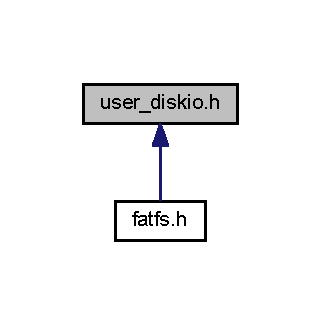
\includegraphics[width=154pt]{user__diskio_8h__dep__incl}
\end{center}
\end{figure}
\subsection*{Variables}
\begin{DoxyCompactItemize}
\item 
Diskio\+\_\+drv\+Type\+Def \mbox{\hyperlink{user__diskio_8h_a07c50f7d5577591438e4585f13994d49}{U\+S\+E\+R\+\_\+\+Driver}}
\end{DoxyCompactItemize}


\subsection{Detailed Description}
This file contains the common defines and functions prototypes for ~\newline
 the user\+\_\+diskio driver. 

This notice applies to any and all portions of this file that are not between comment pairs U\+S\+ER C\+O\+DE B\+E\+G\+IN and U\+S\+ER C\+O\+DE E\+ND. Other portions of this file, whether inserted by the user or by software development tools are owned by their respective copyright owners.

Copyright (c) 2018 S\+T\+Microelectronics International N.\+V. All rights reserved.

Redistribution and use in source and binary forms, with or without modification, are permitted, provided that the following conditions are met\+:


\begin{DoxyEnumerate}
\item Redistribution of source code must retain the above copyright notice, this list of conditions and the following disclaimer.
\item Redistributions in binary form must reproduce the above copyright notice, this list of conditions and the following disclaimer in the documentation and/or other materials provided with the distribution.
\item Neither the name of S\+T\+Microelectronics nor the names of other contributors to this software may be used to endorse or promote products derived from this software without specific written permission.
\item This software, including modifications and/or derivative works of this software, must execute solely and exclusively on microcontroller or microprocessor devices manufactured by or for S\+T\+Microelectronics.
\item Redistribution and use of this software other than as permitted under this license is void and will automatically terminate your rights under this license.
\end{DoxyEnumerate}

T\+H\+IS S\+O\+F\+T\+W\+A\+RE IS P\+R\+O\+V\+I\+D\+ED BY S\+T\+M\+I\+C\+R\+O\+E\+L\+E\+C\+T\+R\+O\+N\+I\+CS A\+ND C\+O\+N\+T\+R\+I\+B\+U\+T\+O\+RS \char`\"{}\+A\+S I\+S\char`\"{} A\+ND A\+NY E\+X\+P\+R\+E\+SS, I\+M\+P\+L\+I\+ED OR S\+T\+A\+T\+U\+T\+O\+RY W\+A\+R\+R\+A\+N\+T\+I\+ES, I\+N\+C\+L\+U\+D\+I\+NG, B\+UT N\+OT L\+I\+M\+I\+T\+ED TO, T\+HE I\+M\+P\+L\+I\+ED W\+A\+R\+R\+A\+N\+T\+I\+ES OF M\+E\+R\+C\+H\+A\+N\+T\+A\+B\+I\+L\+I\+TY, F\+I\+T\+N\+E\+SS F\+OR A P\+A\+R\+T\+I\+C\+U\+L\+AR P\+U\+R\+P\+O\+SE A\+ND N\+O\+N-\/\+I\+N\+F\+R\+I\+N\+G\+E\+M\+E\+NT OF T\+H\+I\+RD P\+A\+R\+TY I\+N\+T\+E\+L\+L\+E\+C\+T\+U\+AL P\+R\+O\+P\+E\+R\+TY R\+I\+G\+H\+TS A\+RE D\+I\+S\+C\+L\+A\+I\+M\+ED TO T\+HE F\+U\+L\+L\+E\+ST E\+X\+T\+E\+NT P\+E\+R\+M\+I\+T\+T\+ED BY L\+AW. IN NO E\+V\+E\+NT S\+H\+A\+LL S\+T\+M\+I\+C\+R\+O\+E\+L\+E\+C\+T\+R\+O\+N\+I\+CS OR C\+O\+N\+T\+R\+I\+B\+U\+T\+O\+RS BE L\+I\+A\+B\+LE F\+OR A\+NY D\+I\+R\+E\+CT, I\+N\+D\+I\+R\+E\+CT, I\+N\+C\+I\+D\+E\+N\+T\+AL, S\+P\+E\+C\+I\+AL, E\+X\+E\+M\+P\+L\+A\+RY, OR C\+O\+N\+S\+E\+Q\+U\+E\+N\+T\+I\+AL D\+A\+M\+A\+G\+ES (I\+N\+C\+L\+U\+D\+I\+NG, B\+UT N\+OT L\+I\+M\+I\+T\+ED TO, P\+R\+O\+C\+U\+R\+E\+M\+E\+NT OF S\+U\+B\+S\+T\+I\+T\+U\+TE G\+O\+O\+DS OR S\+E\+R\+V\+I\+C\+ES; L\+O\+SS OF U\+SE, D\+A\+TA, OR P\+R\+O\+F\+I\+TS; OR B\+U\+S\+I\+N\+E\+SS I\+N\+T\+E\+R\+R\+U\+P\+T\+I\+ON) H\+O\+W\+E\+V\+ER C\+A\+U\+S\+ED A\+ND ON A\+NY T\+H\+E\+O\+RY OF L\+I\+A\+B\+I\+L\+I\+TY, W\+H\+E\+T\+H\+ER IN C\+O\+N\+T\+R\+A\+CT, S\+T\+R\+I\+CT L\+I\+A\+B\+I\+L\+I\+TY, OR T\+O\+RT (I\+N\+C\+L\+U\+D\+I\+NG N\+E\+G\+L\+I\+G\+E\+N\+CE OR O\+T\+H\+E\+R\+W\+I\+SE) A\+R\+I\+S\+I\+NG IN A\+NY W\+AY O\+UT OF T\+HE U\+SE OF T\+H\+IS S\+O\+F\+T\+W\+A\+RE, E\+V\+EN IF A\+D\+V\+I\+S\+ED OF T\+HE P\+O\+S\+S\+I\+B\+I\+L\+I\+TY OF S\+U\+CH D\+A\+M\+A\+GE. 

\subsection{Variable Documentation}
\mbox{\Hypertarget{user__diskio_8h_a07c50f7d5577591438e4585f13994d49}\label{user__diskio_8h_a07c50f7d5577591438e4585f13994d49}} 
\index{user\+\_\+diskio.\+h@{user\+\_\+diskio.\+h}!U\+S\+E\+R\+\_\+\+Driver@{U\+S\+E\+R\+\_\+\+Driver}}
\index{U\+S\+E\+R\+\_\+\+Driver@{U\+S\+E\+R\+\_\+\+Driver}!user\+\_\+diskio.\+h@{user\+\_\+diskio.\+h}}
\subsubsection{\texorpdfstring{U\+S\+E\+R\+\_\+\+Driver}{USER\_Driver}}
{\footnotesize\ttfamily Diskio\+\_\+drv\+Type\+Def U\+S\+E\+R\+\_\+\+Driver}


\hypertarget{button_8h}{}\section{C\+:/\+Users/\+T\+H\+P/\+Desktop/\+Unibern/2018\+\_\+02/\+Subjects/\+Programming\+\_\+\+Microcontroller/\+Paeks/samples/\+My\+\_\+\+Project/\+Library/\+Library/inc/button.h File Reference}
\label{button_8h}\index{C\+:/\+Users/\+T\+H\+P/\+Desktop/\+Unibern/2018\+\_\+02/\+Subjects/\+Programming\+\_\+\+Microcontroller/\+Paeks/samples/\+My\+\_\+\+Project/\+Library/\+Library/inc/button.\+h@{C\+:/\+Users/\+T\+H\+P/\+Desktop/\+Unibern/2018\+\_\+02/\+Subjects/\+Programming\+\_\+\+Microcontroller/\+Paeks/samples/\+My\+\_\+\+Project/\+Library/\+Library/inc/button.\+h}}
{\ttfamily \#include \char`\"{}stdint.\+h\char`\"{}}\newline
{\ttfamily \#include \char`\"{}stdlib.\+h\char`\"{}}\newline
{\ttfamily \#include \char`\"{}stm32f4xx\+\_\+hal.\+h\char`\"{}}\newline
Include dependency graph for button.\+h\+:\nopagebreak
\begin{figure}[H]
\begin{center}
\leavevmode
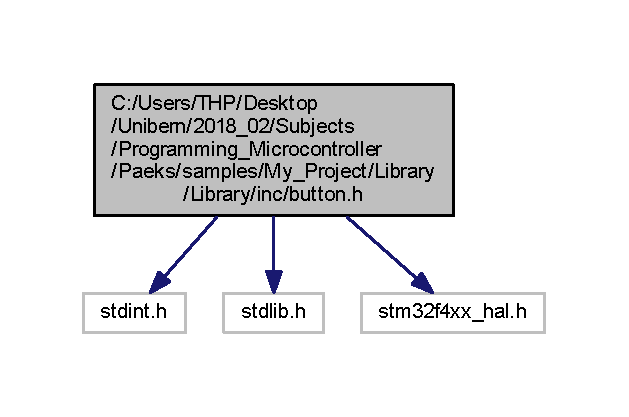
\includegraphics[width=302pt]{button_8h__incl}
\end{center}
\end{figure}
This graph shows which files directly or indirectly include this file\+:\nopagebreak
\begin{figure}[H]
\begin{center}
\leavevmode
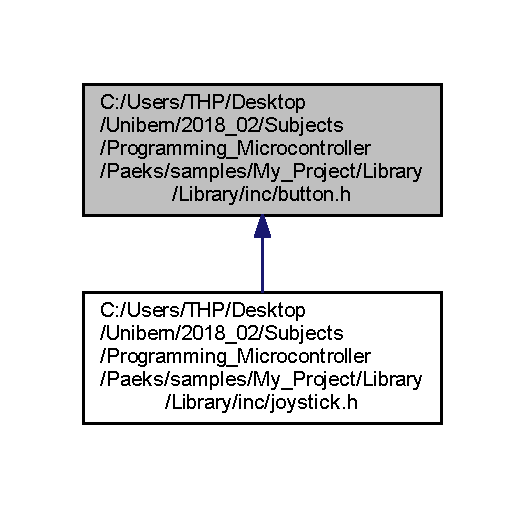
\includegraphics[width=252pt]{button_8h__dep__incl}
\end{center}
\end{figure}
\subsection*{Data Structures}
\begin{DoxyCompactItemize}
\item 
struct \mbox{\hyperlink{struct_button__}{Button\+\_\+}}
\end{DoxyCompactItemize}
\subsection*{Macros}
\begin{DoxyCompactItemize}
\item 
\#define \mbox{\hyperlink{button_8h_ac243bfa96aa2c28014159ff098bd2324}{E\+D\+GE}}
\end{DoxyCompactItemize}
\subsection*{Typedefs}
\begin{DoxyCompactItemize}
\item 
typedef struct \mbox{\hyperlink{struct_input_filter__}{Input\+Filter\+\_\+}} \mbox{\hyperlink{button_8h_aa0f38bbf6320aea7cc99c3a77ed46d80}{Input\+Filter}}
\item 
typedef struct \mbox{\hyperlink{struct_button__}{Button\+\_\+}} \mbox{\hyperlink{button_8h_ab369ab7fa0b9a8dfec4fc1f653ac6de5}{Button}}
\end{DoxyCompactItemize}
\subsection*{Enumerations}
\begin{DoxyCompactItemize}
\item 
enum \mbox{\hyperlink{button_8h_a4ef43ff5c6d42dacbc8ffd9c8cfdc189}{edge}} \{ \newline
\mbox{\hyperlink{button_8h_a4ef43ff5c6d42dacbc8ffd9c8cfdc189ab88c132109a78c131815f270b8bef045}{F\+A\+L\+L\+I\+N\+G\+\_\+\+E\+D\+GE}}, 
\mbox{\hyperlink{button_8h_a4ef43ff5c6d42dacbc8ffd9c8cfdc189a568c13a92a1e1635d9bd20282d67a336}{N\+O\+\_\+\+E\+D\+GE}}, 
\mbox{\hyperlink{button_8h_a4ef43ff5c6d42dacbc8ffd9c8cfdc189a86445853271053ed37f404b9ca4fa434}{R\+I\+S\+I\+N\+G\+\_\+\+E\+D\+GE}}, 
\mbox{\hyperlink{button__driver_8h_a4ef43ff5c6d42dacbc8ffd9c8cfdc189ab88c132109a78c131815f270b8bef045}{F\+A\+L\+L\+I\+N\+G\+\_\+\+E\+D\+GE}}, 
\newline
\mbox{\hyperlink{button__driver_8h_a4ef43ff5c6d42dacbc8ffd9c8cfdc189a568c13a92a1e1635d9bd20282d67a336}{N\+O\+\_\+\+E\+D\+GE}}, 
\mbox{\hyperlink{button__driver_8h_a4ef43ff5c6d42dacbc8ffd9c8cfdc189a86445853271053ed37f404b9ca4fa434}{R\+I\+S\+I\+N\+G\+\_\+\+E\+D\+GE}}
 \}
\end{DoxyCompactItemize}
\subsection*{Functions}
\begin{DoxyCompactItemize}
\item 
uint8\+\_\+t \mbox{\hyperlink{button_8h_af2c0ff777b822ad89ae3df68ca0c5e4b}{Button\+\_\+init}} (\mbox{\hyperlink{button_8h_ab369ab7fa0b9a8dfec4fc1f653ac6de5}{Button}} $\ast$const \+\_\+this, G\+P\+I\+O\+\_\+\+Type\+Def $\ast$const port, uint16\+\_\+t pin)
\end{DoxyCompactItemize}


\subsection{Macro Definition Documentation}
\mbox{\Hypertarget{button_8h_ac243bfa96aa2c28014159ff098bd2324}\label{button_8h_ac243bfa96aa2c28014159ff098bd2324}} 
\index{button.\+h@{button.\+h}!E\+D\+GE@{E\+D\+GE}}
\index{E\+D\+GE@{E\+D\+GE}!button.\+h@{button.\+h}}
\subsubsection{\texorpdfstring{E\+D\+GE}{EDGE}}
{\footnotesize\ttfamily \#define E\+D\+GE}



Definition at line 11 of file button.\+h.



\subsection{Typedef Documentation}
\mbox{\Hypertarget{button_8h_ab369ab7fa0b9a8dfec4fc1f653ac6de5}\label{button_8h_ab369ab7fa0b9a8dfec4fc1f653ac6de5}} 
\index{button.\+h@{button.\+h}!Button@{Button}}
\index{Button@{Button}!button.\+h@{button.\+h}}
\subsubsection{\texorpdfstring{Button}{Button}}
{\footnotesize\ttfamily typedef struct \mbox{\hyperlink{struct_button__}{Button\+\_\+}} \mbox{\hyperlink{button_8h_ab369ab7fa0b9a8dfec4fc1f653ac6de5}{Button}}}

\mbox{\Hypertarget{button_8h_aa0f38bbf6320aea7cc99c3a77ed46d80}\label{button_8h_aa0f38bbf6320aea7cc99c3a77ed46d80}} 
\index{button.\+h@{button.\+h}!Input\+Filter@{Input\+Filter}}
\index{Input\+Filter@{Input\+Filter}!button.\+h@{button.\+h}}
\subsubsection{\texorpdfstring{Input\+Filter}{InputFilter}}
{\footnotesize\ttfamily typedef struct \mbox{\hyperlink{struct_input_filter__}{Input\+Filter\+\_\+}} \mbox{\hyperlink{button_8h_aa0f38bbf6320aea7cc99c3a77ed46d80}{Input\+Filter}}}



Definition at line 8 of file button.\+h.



\subsection{Enumeration Type Documentation}
\mbox{\Hypertarget{button_8h_a4ef43ff5c6d42dacbc8ffd9c8cfdc189}\label{button_8h_a4ef43ff5c6d42dacbc8ffd9c8cfdc189}} 
\index{button.\+h@{button.\+h}!edge@{edge}}
\index{edge@{edge}!button.\+h@{button.\+h}}
\subsubsection{\texorpdfstring{edge}{edge}}
{\footnotesize\ttfamily enum \mbox{\hyperlink{button_8h_a4ef43ff5c6d42dacbc8ffd9c8cfdc189}{edge}}}

\begin{DoxyEnumFields}{Enumerator}
\raisebox{\heightof{T}}[0pt][0pt]{\index{F\+A\+L\+L\+I\+N\+G\+\_\+\+E\+D\+GE@{F\+A\+L\+L\+I\+N\+G\+\_\+\+E\+D\+GE}!button.\+h@{button.\+h}}\index{button.\+h@{button.\+h}!F\+A\+L\+L\+I\+N\+G\+\_\+\+E\+D\+GE@{F\+A\+L\+L\+I\+N\+G\+\_\+\+E\+D\+GE}}}\mbox{\Hypertarget{button_8h_a4ef43ff5c6d42dacbc8ffd9c8cfdc189ab88c132109a78c131815f270b8bef045}\label{button_8h_a4ef43ff5c6d42dacbc8ffd9c8cfdc189ab88c132109a78c131815f270b8bef045}} 
F\+A\+L\+L\+I\+N\+G\+\_\+\+E\+D\+GE&\\
\hline

\raisebox{\heightof{T}}[0pt][0pt]{\index{N\+O\+\_\+\+E\+D\+GE@{N\+O\+\_\+\+E\+D\+GE}!button.\+h@{button.\+h}}\index{button.\+h@{button.\+h}!N\+O\+\_\+\+E\+D\+GE@{N\+O\+\_\+\+E\+D\+GE}}}\mbox{\Hypertarget{button_8h_a4ef43ff5c6d42dacbc8ffd9c8cfdc189a568c13a92a1e1635d9bd20282d67a336}\label{button_8h_a4ef43ff5c6d42dacbc8ffd9c8cfdc189a568c13a92a1e1635d9bd20282d67a336}} 
N\+O\+\_\+\+E\+D\+GE&\\
\hline

\raisebox{\heightof{T}}[0pt][0pt]{\index{R\+I\+S\+I\+N\+G\+\_\+\+E\+D\+GE@{R\+I\+S\+I\+N\+G\+\_\+\+E\+D\+GE}!button.\+h@{button.\+h}}\index{button.\+h@{button.\+h}!R\+I\+S\+I\+N\+G\+\_\+\+E\+D\+GE@{R\+I\+S\+I\+N\+G\+\_\+\+E\+D\+GE}}}\mbox{\Hypertarget{button_8h_a4ef43ff5c6d42dacbc8ffd9c8cfdc189a86445853271053ed37f404b9ca4fa434}\label{button_8h_a4ef43ff5c6d42dacbc8ffd9c8cfdc189a86445853271053ed37f404b9ca4fa434}} 
R\+I\+S\+I\+N\+G\+\_\+\+E\+D\+GE&\\
\hline

\raisebox{\heightof{T}}[0pt][0pt]{\index{F\+A\+L\+L\+I\+N\+G\+\_\+\+E\+D\+GE@{F\+A\+L\+L\+I\+N\+G\+\_\+\+E\+D\+GE}!button.\+h@{button.\+h}}\index{button.\+h@{button.\+h}!F\+A\+L\+L\+I\+N\+G\+\_\+\+E\+D\+GE@{F\+A\+L\+L\+I\+N\+G\+\_\+\+E\+D\+GE}}}\mbox{\Hypertarget{button_8h_a4ef43ff5c6d42dacbc8ffd9c8cfdc189ab88c132109a78c131815f270b8bef045}\label{button_8h_a4ef43ff5c6d42dacbc8ffd9c8cfdc189ab88c132109a78c131815f270b8bef045}} 
F\+A\+L\+L\+I\+N\+G\+\_\+\+E\+D\+GE&\\
\hline

\raisebox{\heightof{T}}[0pt][0pt]{\index{N\+O\+\_\+\+E\+D\+GE@{N\+O\+\_\+\+E\+D\+GE}!button.\+h@{button.\+h}}\index{button.\+h@{button.\+h}!N\+O\+\_\+\+E\+D\+GE@{N\+O\+\_\+\+E\+D\+GE}}}\mbox{\Hypertarget{button_8h_a4ef43ff5c6d42dacbc8ffd9c8cfdc189a568c13a92a1e1635d9bd20282d67a336}\label{button_8h_a4ef43ff5c6d42dacbc8ffd9c8cfdc189a568c13a92a1e1635d9bd20282d67a336}} 
N\+O\+\_\+\+E\+D\+GE&\\
\hline

\raisebox{\heightof{T}}[0pt][0pt]{\index{R\+I\+S\+I\+N\+G\+\_\+\+E\+D\+GE@{R\+I\+S\+I\+N\+G\+\_\+\+E\+D\+GE}!button.\+h@{button.\+h}}\index{button.\+h@{button.\+h}!R\+I\+S\+I\+N\+G\+\_\+\+E\+D\+GE@{R\+I\+S\+I\+N\+G\+\_\+\+E\+D\+GE}}}\mbox{\Hypertarget{button_8h_a4ef43ff5c6d42dacbc8ffd9c8cfdc189a86445853271053ed37f404b9ca4fa434}\label{button_8h_a4ef43ff5c6d42dacbc8ffd9c8cfdc189a86445853271053ed37f404b9ca4fa434}} 
R\+I\+S\+I\+N\+G\+\_\+\+E\+D\+GE&\\
\hline

\end{DoxyEnumFields}


Definition at line 12 of file button.\+h.



\subsection{Function Documentation}
\mbox{\Hypertarget{button_8h_af2c0ff777b822ad89ae3df68ca0c5e4b}\label{button_8h_af2c0ff777b822ad89ae3df68ca0c5e4b}} 
\index{button.\+h@{button.\+h}!Button\+\_\+init@{Button\+\_\+init}}
\index{Button\+\_\+init@{Button\+\_\+init}!button.\+h@{button.\+h}}
\subsubsection{\texorpdfstring{Button\+\_\+init()}{Button\_init()}}
{\footnotesize\ttfamily uint8\+\_\+t Button\+\_\+init (\begin{DoxyParamCaption}\item[{\mbox{\hyperlink{button_8h_ab369ab7fa0b9a8dfec4fc1f653ac6de5}{Button}} $\ast$const}]{\+\_\+this,  }\item[{G\+P\+I\+O\+\_\+\+Type\+Def $\ast$const}]{port,  }\item[{uint16\+\_\+t}]{pin }\end{DoxyParamCaption})}


\hypertarget{button__driver_8h}{}\section{C\+:/\+Users/\+T\+H\+P/\+Desktop/\+Unibern/2018\+\_\+02/\+Subjects/\+Programming\+\_\+\+Microcontroller/\+Paeks/samples/\+My\+\_\+\+Project/\+Library/\+Library/inc/button\+\_\+driver.h File Reference}
\label{button__driver_8h}\index{C\+:/\+Users/\+T\+H\+P/\+Desktop/\+Unibern/2018\+\_\+02/\+Subjects/\+Programming\+\_\+\+Microcontroller/\+Paeks/samples/\+My\+\_\+\+Project/\+Library/\+Library/inc/button\+\_\+driver.\+h@{C\+:/\+Users/\+T\+H\+P/\+Desktop/\+Unibern/2018\+\_\+02/\+Subjects/\+Programming\+\_\+\+Microcontroller/\+Paeks/samples/\+My\+\_\+\+Project/\+Library/\+Library/inc/button\+\_\+driver.\+h}}
{\ttfamily \#include \char`\"{}stm32f4xx\+\_\+hal.\+h\char`\"{}}\newline
{\ttfamily \#include \char`\"{}stdbool.\+h\char`\"{}}\newline
{\ttfamily \#include \char`\"{}stdlib.\+h\char`\"{}}\newline
{\ttfamily \#include \char`\"{}stdint.\+h\char`\"{}}\newline
Include dependency graph for button\+\_\+driver.\+h\+:\nopagebreak
\begin{figure}[H]
\begin{center}
\leavevmode
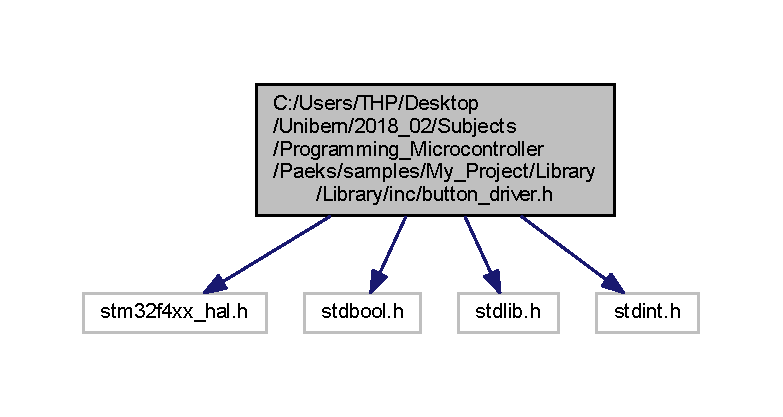
\includegraphics[width=350pt]{button__driver_8h__incl}
\end{center}
\end{figure}
\subsection*{Data Structures}
\begin{DoxyCompactItemize}
\item 
struct \mbox{\hyperlink{struct_input_filter__}{Input\+Filter\+\_\+}}
\end{DoxyCompactItemize}
\subsection*{Macros}
\begin{DoxyCompactItemize}
\item 
\#define \mbox{\hyperlink{button__driver_8h_a15336ba289605e6744d084ae8e4f37cc}{I\+N\+P\+U\+T\+\_\+\+L\+OW}}~((uint16\+\_\+t)  0)
\item 
\#define \mbox{\hyperlink{button__driver_8h_a36700c52f8a492d9045ceacdd6b98101}{I\+N\+P\+U\+T\+\_\+\+H\+I\+GH}}~((uint16\+\_\+t)  65535)
\item 
\#define \mbox{\hyperlink{button__driver_8h_ac243bfa96aa2c28014159ff098bd2324}{E\+D\+GE}}
\end{DoxyCompactItemize}
\subsection*{Typedefs}
\begin{DoxyCompactItemize}
\item 
typedef struct \mbox{\hyperlink{struct_input_filter__}{Input\+Filter\+\_\+}} \mbox{\hyperlink{button__driver_8h_aa0f38bbf6320aea7cc99c3a77ed46d80}{Input\+Filter}}
\end{DoxyCompactItemize}
\subsection*{Enumerations}
\begin{DoxyCompactItemize}
\item 
enum \mbox{\hyperlink{button__driver_8h_a4ef43ff5c6d42dacbc8ffd9c8cfdc189}{edge}} \{ \newline
\mbox{\hyperlink{button_8h_a4ef43ff5c6d42dacbc8ffd9c8cfdc189ab88c132109a78c131815f270b8bef045}{F\+A\+L\+L\+I\+N\+G\+\_\+\+E\+D\+GE}}, 
\mbox{\hyperlink{button_8h_a4ef43ff5c6d42dacbc8ffd9c8cfdc189a568c13a92a1e1635d9bd20282d67a336}{N\+O\+\_\+\+E\+D\+GE}}, 
\mbox{\hyperlink{button_8h_a4ef43ff5c6d42dacbc8ffd9c8cfdc189a86445853271053ed37f404b9ca4fa434}{R\+I\+S\+I\+N\+G\+\_\+\+E\+D\+GE}}, 
\mbox{\hyperlink{button__driver_8h_a4ef43ff5c6d42dacbc8ffd9c8cfdc189ab88c132109a78c131815f270b8bef045}{F\+A\+L\+L\+I\+N\+G\+\_\+\+E\+D\+GE}}, 
\newline
\mbox{\hyperlink{button__driver_8h_a4ef43ff5c6d42dacbc8ffd9c8cfdc189a568c13a92a1e1635d9bd20282d67a336}{N\+O\+\_\+\+E\+D\+GE}}, 
\mbox{\hyperlink{button__driver_8h_a4ef43ff5c6d42dacbc8ffd9c8cfdc189a86445853271053ed37f404b9ca4fa434}{R\+I\+S\+I\+N\+G\+\_\+\+E\+D\+GE}}
 \}
\end{DoxyCompactItemize}
\subsection*{Functions}
\begin{DoxyCompactItemize}
\item 
uint8\+\_\+t \mbox{\hyperlink{button__driver_8h_a61dbff7d557fc276d145eddf49b0bbe1}{Input\+Filter\+\_\+init}} (\mbox{\hyperlink{button_8h_aa0f38bbf6320aea7cc99c3a77ed46d80}{Input\+Filter}} $\ast$const \+\_\+this, G\+P\+I\+O\+\_\+\+Type\+Def $\ast$const port, uint16\+\_\+t pin)
\end{DoxyCompactItemize}


\subsection{Macro Definition Documentation}
\mbox{\Hypertarget{button__driver_8h_ac243bfa96aa2c28014159ff098bd2324}\label{button__driver_8h_ac243bfa96aa2c28014159ff098bd2324}} 
\index{button\+\_\+driver.\+h@{button\+\_\+driver.\+h}!E\+D\+GE@{E\+D\+GE}}
\index{E\+D\+GE@{E\+D\+GE}!button\+\_\+driver.\+h@{button\+\_\+driver.\+h}}
\subsubsection{\texorpdfstring{E\+D\+GE}{EDGE}}
{\footnotesize\ttfamily \#define E\+D\+GE}



Definition at line 14 of file button\+\_\+driver.\+h.

\mbox{\Hypertarget{button__driver_8h_a36700c52f8a492d9045ceacdd6b98101}\label{button__driver_8h_a36700c52f8a492d9045ceacdd6b98101}} 
\index{button\+\_\+driver.\+h@{button\+\_\+driver.\+h}!I\+N\+P\+U\+T\+\_\+\+H\+I\+GH@{I\+N\+P\+U\+T\+\_\+\+H\+I\+GH}}
\index{I\+N\+P\+U\+T\+\_\+\+H\+I\+GH@{I\+N\+P\+U\+T\+\_\+\+H\+I\+GH}!button\+\_\+driver.\+h@{button\+\_\+driver.\+h}}
\subsubsection{\texorpdfstring{I\+N\+P\+U\+T\+\_\+\+H\+I\+GH}{INPUT\_HIGH}}
{\footnotesize\ttfamily \#define I\+N\+P\+U\+T\+\_\+\+H\+I\+GH~((uint16\+\_\+t)  65535)}



Definition at line 10 of file button\+\_\+driver.\+h.

\mbox{\Hypertarget{button__driver_8h_a15336ba289605e6744d084ae8e4f37cc}\label{button__driver_8h_a15336ba289605e6744d084ae8e4f37cc}} 
\index{button\+\_\+driver.\+h@{button\+\_\+driver.\+h}!I\+N\+P\+U\+T\+\_\+\+L\+OW@{I\+N\+P\+U\+T\+\_\+\+L\+OW}}
\index{I\+N\+P\+U\+T\+\_\+\+L\+OW@{I\+N\+P\+U\+T\+\_\+\+L\+OW}!button\+\_\+driver.\+h@{button\+\_\+driver.\+h}}
\subsubsection{\texorpdfstring{I\+N\+P\+U\+T\+\_\+\+L\+OW}{INPUT\_LOW}}
{\footnotesize\ttfamily \#define I\+N\+P\+U\+T\+\_\+\+L\+OW~((uint16\+\_\+t)  0)}



Definition at line 9 of file button\+\_\+driver.\+h.



\subsection{Typedef Documentation}
\mbox{\Hypertarget{button__driver_8h_aa0f38bbf6320aea7cc99c3a77ed46d80}\label{button__driver_8h_aa0f38bbf6320aea7cc99c3a77ed46d80}} 
\index{button\+\_\+driver.\+h@{button\+\_\+driver.\+h}!Input\+Filter@{Input\+Filter}}
\index{Input\+Filter@{Input\+Filter}!button\+\_\+driver.\+h@{button\+\_\+driver.\+h}}
\subsubsection{\texorpdfstring{Input\+Filter}{InputFilter}}
{\footnotesize\ttfamily typedef struct \mbox{\hyperlink{struct_input_filter__}{Input\+Filter\+\_\+}} \mbox{\hyperlink{button_8h_aa0f38bbf6320aea7cc99c3a77ed46d80}{Input\+Filter}}}



\subsection{Enumeration Type Documentation}
\mbox{\Hypertarget{button__driver_8h_a4ef43ff5c6d42dacbc8ffd9c8cfdc189}\label{button__driver_8h_a4ef43ff5c6d42dacbc8ffd9c8cfdc189}} 
\index{button\+\_\+driver.\+h@{button\+\_\+driver.\+h}!edge@{edge}}
\index{edge@{edge}!button\+\_\+driver.\+h@{button\+\_\+driver.\+h}}
\subsubsection{\texorpdfstring{edge}{edge}}
{\footnotesize\ttfamily enum \mbox{\hyperlink{button_8h_a4ef43ff5c6d42dacbc8ffd9c8cfdc189}{edge}}}

\begin{DoxyEnumFields}{Enumerator}
\raisebox{\heightof{T}}[0pt][0pt]{\index{F\+A\+L\+L\+I\+N\+G\+\_\+\+E\+D\+GE@{F\+A\+L\+L\+I\+N\+G\+\_\+\+E\+D\+GE}!button\+\_\+driver.\+h@{button\+\_\+driver.\+h}}\index{button\+\_\+driver.\+h@{button\+\_\+driver.\+h}!F\+A\+L\+L\+I\+N\+G\+\_\+\+E\+D\+GE@{F\+A\+L\+L\+I\+N\+G\+\_\+\+E\+D\+GE}}}\mbox{\Hypertarget{button__driver_8h_a4ef43ff5c6d42dacbc8ffd9c8cfdc189ab88c132109a78c131815f270b8bef045}\label{button__driver_8h_a4ef43ff5c6d42dacbc8ffd9c8cfdc189ab88c132109a78c131815f270b8bef045}} 
F\+A\+L\+L\+I\+N\+G\+\_\+\+E\+D\+GE&\\
\hline

\raisebox{\heightof{T}}[0pt][0pt]{\index{N\+O\+\_\+\+E\+D\+GE@{N\+O\+\_\+\+E\+D\+GE}!button\+\_\+driver.\+h@{button\+\_\+driver.\+h}}\index{button\+\_\+driver.\+h@{button\+\_\+driver.\+h}!N\+O\+\_\+\+E\+D\+GE@{N\+O\+\_\+\+E\+D\+GE}}}\mbox{\Hypertarget{button__driver_8h_a4ef43ff5c6d42dacbc8ffd9c8cfdc189a568c13a92a1e1635d9bd20282d67a336}\label{button__driver_8h_a4ef43ff5c6d42dacbc8ffd9c8cfdc189a568c13a92a1e1635d9bd20282d67a336}} 
N\+O\+\_\+\+E\+D\+GE&\\
\hline

\raisebox{\heightof{T}}[0pt][0pt]{\index{R\+I\+S\+I\+N\+G\+\_\+\+E\+D\+GE@{R\+I\+S\+I\+N\+G\+\_\+\+E\+D\+GE}!button\+\_\+driver.\+h@{button\+\_\+driver.\+h}}\index{button\+\_\+driver.\+h@{button\+\_\+driver.\+h}!R\+I\+S\+I\+N\+G\+\_\+\+E\+D\+GE@{R\+I\+S\+I\+N\+G\+\_\+\+E\+D\+GE}}}\mbox{\Hypertarget{button__driver_8h_a4ef43ff5c6d42dacbc8ffd9c8cfdc189a86445853271053ed37f404b9ca4fa434}\label{button__driver_8h_a4ef43ff5c6d42dacbc8ffd9c8cfdc189a86445853271053ed37f404b9ca4fa434}} 
R\+I\+S\+I\+N\+G\+\_\+\+E\+D\+GE&\\
\hline

\raisebox{\heightof{T}}[0pt][0pt]{\index{F\+A\+L\+L\+I\+N\+G\+\_\+\+E\+D\+GE@{F\+A\+L\+L\+I\+N\+G\+\_\+\+E\+D\+GE}!button\+\_\+driver.\+h@{button\+\_\+driver.\+h}}\index{button\+\_\+driver.\+h@{button\+\_\+driver.\+h}!F\+A\+L\+L\+I\+N\+G\+\_\+\+E\+D\+GE@{F\+A\+L\+L\+I\+N\+G\+\_\+\+E\+D\+GE}}}\mbox{\Hypertarget{button__driver_8h_a4ef43ff5c6d42dacbc8ffd9c8cfdc189ab88c132109a78c131815f270b8bef045}\label{button__driver_8h_a4ef43ff5c6d42dacbc8ffd9c8cfdc189ab88c132109a78c131815f270b8bef045}} 
F\+A\+L\+L\+I\+N\+G\+\_\+\+E\+D\+GE&\\
\hline

\raisebox{\heightof{T}}[0pt][0pt]{\index{N\+O\+\_\+\+E\+D\+GE@{N\+O\+\_\+\+E\+D\+GE}!button\+\_\+driver.\+h@{button\+\_\+driver.\+h}}\index{button\+\_\+driver.\+h@{button\+\_\+driver.\+h}!N\+O\+\_\+\+E\+D\+GE@{N\+O\+\_\+\+E\+D\+GE}}}\mbox{\Hypertarget{button__driver_8h_a4ef43ff5c6d42dacbc8ffd9c8cfdc189a568c13a92a1e1635d9bd20282d67a336}\label{button__driver_8h_a4ef43ff5c6d42dacbc8ffd9c8cfdc189a568c13a92a1e1635d9bd20282d67a336}} 
N\+O\+\_\+\+E\+D\+GE&\\
\hline

\raisebox{\heightof{T}}[0pt][0pt]{\index{R\+I\+S\+I\+N\+G\+\_\+\+E\+D\+GE@{R\+I\+S\+I\+N\+G\+\_\+\+E\+D\+GE}!button\+\_\+driver.\+h@{button\+\_\+driver.\+h}}\index{button\+\_\+driver.\+h@{button\+\_\+driver.\+h}!R\+I\+S\+I\+N\+G\+\_\+\+E\+D\+GE@{R\+I\+S\+I\+N\+G\+\_\+\+E\+D\+GE}}}\mbox{\Hypertarget{button__driver_8h_a4ef43ff5c6d42dacbc8ffd9c8cfdc189a86445853271053ed37f404b9ca4fa434}\label{button__driver_8h_a4ef43ff5c6d42dacbc8ffd9c8cfdc189a86445853271053ed37f404b9ca4fa434}} 
R\+I\+S\+I\+N\+G\+\_\+\+E\+D\+GE&\\
\hline

\end{DoxyEnumFields}


Definition at line 15 of file button\+\_\+driver.\+h.



\subsection{Function Documentation}
\mbox{\Hypertarget{button__driver_8h_a61dbff7d557fc276d145eddf49b0bbe1}\label{button__driver_8h_a61dbff7d557fc276d145eddf49b0bbe1}} 
\index{button\+\_\+driver.\+h@{button\+\_\+driver.\+h}!Input\+Filter\+\_\+init@{Input\+Filter\+\_\+init}}
\index{Input\+Filter\+\_\+init@{Input\+Filter\+\_\+init}!button\+\_\+driver.\+h@{button\+\_\+driver.\+h}}
\subsubsection{\texorpdfstring{Input\+Filter\+\_\+init()}{InputFilter\_init()}}
{\footnotesize\ttfamily uint8\+\_\+t Input\+Filter\+\_\+init (\begin{DoxyParamCaption}\item[{\mbox{\hyperlink{button_8h_aa0f38bbf6320aea7cc99c3a77ed46d80}{Input\+Filter}} $\ast$const}]{\+\_\+this,  }\item[{G\+P\+I\+O\+\_\+\+Type\+Def $\ast$const}]{port,  }\item[{uint16\+\_\+t}]{pin }\end{DoxyParamCaption})}


\hypertarget{filter__math__pincinato_8h}{}\section{Library/\+Library/inc/filter\+\_\+math\+\_\+pincinato.h File Reference}
\label{filter__math__pincinato_8h}\index{Library/\+Library/inc/filter\+\_\+math\+\_\+pincinato.\+h@{Library/\+Library/inc/filter\+\_\+math\+\_\+pincinato.\+h}}
{\ttfamily \#include $<$stdbool.\+h$>$}\newline
{\ttfamily \#include $<$stdint.\+h$>$}\newline
Include dependency graph for filter\+\_\+math\+\_\+pincinato.\+h\+:\nopagebreak
\begin{figure}[H]
\begin{center}
\leavevmode
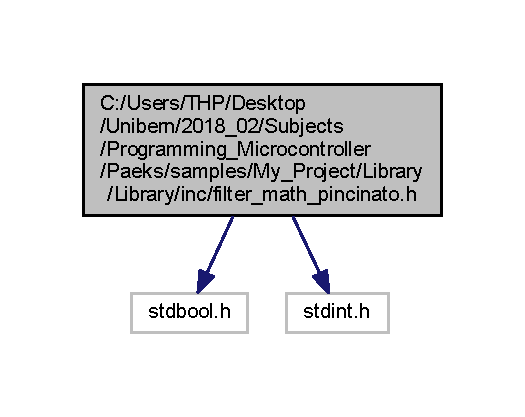
\includegraphics[width=204pt]{filter__math__pincinato_8h__incl}
\end{center}
\end{figure}
This graph shows which files directly or indirectly include this file\+:\nopagebreak
\begin{figure}[H]
\begin{center}
\leavevmode
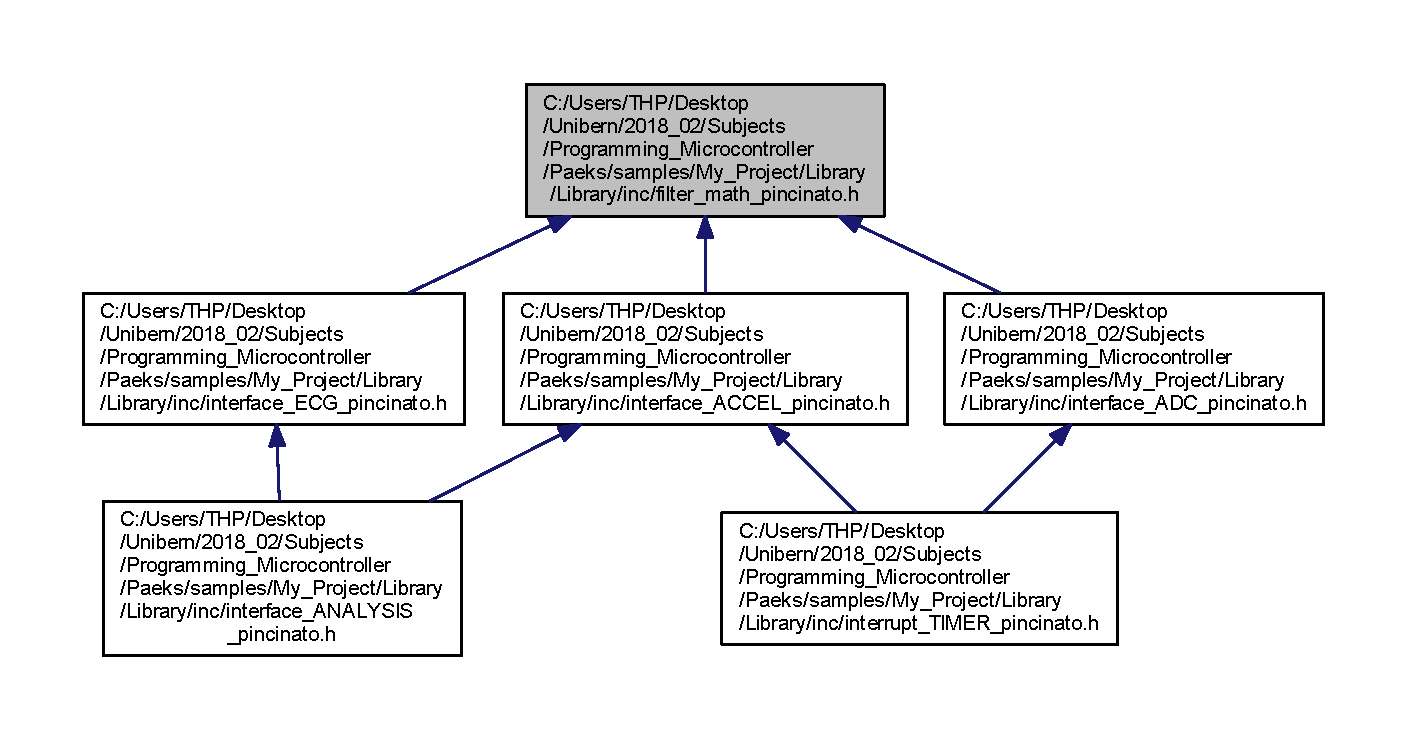
\includegraphics[width=350pt]{filter__math__pincinato_8h__dep__incl}
\end{center}
\end{figure}
\subsection*{Data Structures}
\begin{DoxyCompactItemize}
\item 
struct \mbox{\hyperlink{struct_biquads_filter__}{Biquads\+Filter\+\_\+}}
\item 
struct \mbox{\hyperlink{struct_average_filter__}{Average\+Filter\+\_\+}}
\item 
struct \mbox{\hyperlink{struct___integratal_data__}{\+\_\+\+Integratal\+Data\+\_\+}}
\end{DoxyCompactItemize}
\subsection*{Typedefs}
\begin{DoxyCompactItemize}
\item 
typedef struct \mbox{\hyperlink{struct_biquads_filter__}{Biquads\+Filter\+\_\+}} \mbox{\hyperlink{filter__math__pincinato_8h_a431282902bc1cfeb168d1acf574331bb}{Biquads\+Filter}}
\item 
typedef struct \mbox{\hyperlink{struct_average_filter__}{Average\+Filter\+\_\+}} \mbox{\hyperlink{filter__math__pincinato_8h_a05751bcbb0782121ff05ae3b7fc37dac}{Average\+Filter}}
\item 
typedef struct \mbox{\hyperlink{struct___integratal_data__}{\+\_\+\+Integratal\+Data\+\_\+}} \mbox{\hyperlink{filter__math__pincinato_8h_a614628710e855bdeb4949c83265e87e6}{Integration\+Data}}
\end{DoxyCompactItemize}
\subsection*{Functions}
\begin{DoxyCompactItemize}
\item 
void \mbox{\hyperlink{filter__math__pincinato_8h_a0943af2024c7552aed64fe01f1bd8e15}{normalize}} (float $\ast$vec, int size)
\begin{DoxyCompactList}\small\item\em normalize Normalize a arry of float value \end{DoxyCompactList}\item 
void \mbox{\hyperlink{filter__math__pincinato_8h_a1e56653839d2baf5ac7f9f2c315e0d3f}{init\+Biquads\+Filter}} (\mbox{\hyperlink{filter__math__pincinato_8h_a431282902bc1cfeb168d1acf574331bb}{Biquads\+Filter}} $\ast$filter, float $\ast$d\+\_\+data, int size\+Buffer, float Acoef\mbox{[}$\,$\mbox{]}, float Bcoef\mbox{[}$\,$\mbox{]})
\begin{DoxyCompactList}\small\item\em init\+Biquads\+Filter init filter parameters and pointer to respective data \end{DoxyCompactList}\item 
float \mbox{\hyperlink{filter__math__pincinato_8h_a27ddcf224a294fc542ec5484c6b890bb}{filter\+Biquads\+Compute}} (\mbox{\hyperlink{filter__math__pincinato_8h_a431282902bc1cfeb168d1acf574331bb}{Biquads\+Filter}} $\ast$filter, uint32\+\_\+t value)
\begin{DoxyCompactList}\small\item\em filter\+Biquads\+Compute Include the value in the filter and compute the filter operation \end{DoxyCompactList}\item 
void \mbox{\hyperlink{filter__math__pincinato_8h_a19f7f1bff5682407199b7be0a56bc415}{clear\+Biquads\+Filter}} (\mbox{\hyperlink{filter__math__pincinato_8h_a431282902bc1cfeb168d1acf574331bb}{Biquads\+Filter}} $\ast$filter)
\begin{DoxyCompactList}\small\item\em clear\+Biquads\+Filter Set all entry to zero \end{DoxyCompactList}\item 
void \mbox{\hyperlink{filter__math__pincinato_8h_ae7f97bd805fd61dd0a6bf31e92160672}{init\+Average\+Filter}} (\mbox{\hyperlink{filter__math__pincinato_8h_a05751bcbb0782121ff05ae3b7fc37dac}{Average\+Filter}} $\ast$filter, float $\ast$d\+\_\+data, int size\+Buffer)
\begin{DoxyCompactList}\small\item\em init\+Average\+Filter init filter parameters and pointer to respective data \end{DoxyCompactList}\item 
void \mbox{\hyperlink{filter__math__pincinato_8h_a9d94b029f2d1ca252c8cdc925ef9c492}{clear\+Average\+Filter}} (\mbox{\hyperlink{filter__math__pincinato_8h_a05751bcbb0782121ff05ae3b7fc37dac}{Average\+Filter}} $\ast$filter, float inital\+Value)
\begin{DoxyCompactList}\small\item\em clear\+Average\+Filter Set all entry to init value \end{DoxyCompactList}\item 
float \mbox{\hyperlink{filter__math__pincinato_8h_a63b52e2d6e8763a3cb94cd22bde95731}{filter\+Average\+Compute}} (\mbox{\hyperlink{filter__math__pincinato_8h_a05751bcbb0782121ff05ae3b7fc37dac}{Average\+Filter}} $\ast$filter, float value)
\begin{DoxyCompactList}\small\item\em filter\+Average\+Compute include the value in the filter and compute the average \end{DoxyCompactList}\item 
float \mbox{\hyperlink{filter__math__pincinato_8h_ad38cea898eb6470b1635c10c349e2123}{integration\+Relative\+Distance}} (\mbox{\hyperlink{filter__math__pincinato_8h_a614628710e855bdeb4949c83265e87e6}{Integration\+Data}} $\ast$integral, float n)
\begin{DoxyCompactList}\small\item\em integration\+Relative\+Distance Integrates values, regardingless the signal.\+No negative values in the integration. \end{DoxyCompactList}\item 
float \mbox{\hyperlink{filter__math__pincinato_8h_a59bc40beff6775ed45d464b5d9d1870a}{integration\+Compute}} (\mbox{\hyperlink{filter__math__pincinato_8h_a614628710e855bdeb4949c83265e87e6}{Integration\+Data}} $\ast$integral, float n)
\begin{DoxyCompactList}\small\item\em integration\+Compute include the value in the integration and compute the integration \end{DoxyCompactList}\item 
void \mbox{\hyperlink{filter__math__pincinato_8h_a5c31ca586593b15d003e69b87986d9ec}{init\+Integration}} (\mbox{\hyperlink{filter__math__pincinato_8h_a614628710e855bdeb4949c83265e87e6}{Integration\+Data}} $\ast$integration, float $\ast$d\+\_\+data, int size\+Buffer, float time)
\begin{DoxyCompactList}\small\item\em init\+Integration initializes the Integration\+Data parameters and pointer to respective data \end{DoxyCompactList}\item 
void \mbox{\hyperlink{filter__math__pincinato_8h_ab6bd98a7ea0dac0508536be926f14d1e}{clear\+Integration}} (\mbox{\hyperlink{filter__math__pincinato_8h_a614628710e855bdeb4949c83265e87e6}{Integration\+Data}} $\ast$integration)
\begin{DoxyCompactList}\small\item\em clear\+Integration Set all entry to zero \end{DoxyCompactList}\end{DoxyCompactItemize}


\subsection{Typedef Documentation}
\mbox{\Hypertarget{filter__math__pincinato_8h_a05751bcbb0782121ff05ae3b7fc37dac}\label{filter__math__pincinato_8h_a05751bcbb0782121ff05ae3b7fc37dac}} 
\index{filter\+\_\+math\+\_\+pincinato.\+h@{filter\+\_\+math\+\_\+pincinato.\+h}!Average\+Filter@{Average\+Filter}}
\index{Average\+Filter@{Average\+Filter}!filter\+\_\+math\+\_\+pincinato.\+h@{filter\+\_\+math\+\_\+pincinato.\+h}}
\subsubsection{\texorpdfstring{Average\+Filter}{AverageFilter}}
{\footnotesize\ttfamily typedef struct \mbox{\hyperlink{struct_average_filter__}{Average\+Filter\+\_\+}}  \mbox{\hyperlink{filter__math__pincinato_8h_a05751bcbb0782121ff05ae3b7fc37dac}{Average\+Filter}}}

\mbox{\Hypertarget{filter__math__pincinato_8h_a431282902bc1cfeb168d1acf574331bb}\label{filter__math__pincinato_8h_a431282902bc1cfeb168d1acf574331bb}} 
\index{filter\+\_\+math\+\_\+pincinato.\+h@{filter\+\_\+math\+\_\+pincinato.\+h}!Biquads\+Filter@{Biquads\+Filter}}
\index{Biquads\+Filter@{Biquads\+Filter}!filter\+\_\+math\+\_\+pincinato.\+h@{filter\+\_\+math\+\_\+pincinato.\+h}}
\subsubsection{\texorpdfstring{Biquads\+Filter}{BiquadsFilter}}
{\footnotesize\ttfamily typedef struct \mbox{\hyperlink{struct_biquads_filter__}{Biquads\+Filter\+\_\+}}  \mbox{\hyperlink{filter__math__pincinato_8h_a431282902bc1cfeb168d1acf574331bb}{Biquads\+Filter}}}

\mbox{\Hypertarget{filter__math__pincinato_8h_a614628710e855bdeb4949c83265e87e6}\label{filter__math__pincinato_8h_a614628710e855bdeb4949c83265e87e6}} 
\index{filter\+\_\+math\+\_\+pincinato.\+h@{filter\+\_\+math\+\_\+pincinato.\+h}!Integration\+Data@{Integration\+Data}}
\index{Integration\+Data@{Integration\+Data}!filter\+\_\+math\+\_\+pincinato.\+h@{filter\+\_\+math\+\_\+pincinato.\+h}}
\subsubsection{\texorpdfstring{Integration\+Data}{IntegrationData}}
{\footnotesize\ttfamily typedef struct \mbox{\hyperlink{struct___integratal_data__}{\+\_\+\+Integratal\+Data\+\_\+}}  \mbox{\hyperlink{filter__math__pincinato_8h_a614628710e855bdeb4949c83265e87e6}{Integration\+Data}}}



\subsection{Function Documentation}
\mbox{\Hypertarget{filter__math__pincinato_8h_a9d94b029f2d1ca252c8cdc925ef9c492}\label{filter__math__pincinato_8h_a9d94b029f2d1ca252c8cdc925ef9c492}} 
\index{filter\+\_\+math\+\_\+pincinato.\+h@{filter\+\_\+math\+\_\+pincinato.\+h}!clear\+Average\+Filter@{clear\+Average\+Filter}}
\index{clear\+Average\+Filter@{clear\+Average\+Filter}!filter\+\_\+math\+\_\+pincinato.\+h@{filter\+\_\+math\+\_\+pincinato.\+h}}
\subsubsection{\texorpdfstring{clear\+Average\+Filter()}{clearAverageFilter()}}
{\footnotesize\ttfamily void clear\+Average\+Filter (\begin{DoxyParamCaption}\item[{\mbox{\hyperlink{filter__math__pincinato_8h_a05751bcbb0782121ff05ae3b7fc37dac}{Average\+Filter}} $\ast$}]{filter,  }\item[{float}]{inital\+Value }\end{DoxyParamCaption})}



clear\+Average\+Filter Set all entry to init value 


\begin{DoxyParams}{Parameters}
{\em filter} & filter to be cleared \\
\hline
{\em inital\+Value} & float value that will be used to initialize \\
\hline
\end{DoxyParams}


Definition at line 76 of file filter\+\_\+math\+\_\+pincinato.\+c.

\mbox{\Hypertarget{filter__math__pincinato_8h_a19f7f1bff5682407199b7be0a56bc415}\label{filter__math__pincinato_8h_a19f7f1bff5682407199b7be0a56bc415}} 
\index{filter\+\_\+math\+\_\+pincinato.\+h@{filter\+\_\+math\+\_\+pincinato.\+h}!clear\+Biquads\+Filter@{clear\+Biquads\+Filter}}
\index{clear\+Biquads\+Filter@{clear\+Biquads\+Filter}!filter\+\_\+math\+\_\+pincinato.\+h@{filter\+\_\+math\+\_\+pincinato.\+h}}
\subsubsection{\texorpdfstring{clear\+Biquads\+Filter()}{clearBiquadsFilter()}}
{\footnotesize\ttfamily void clear\+Biquads\+Filter (\begin{DoxyParamCaption}\item[{\mbox{\hyperlink{filter__math__pincinato_8h_a431282902bc1cfeb168d1acf574331bb}{Biquads\+Filter}} $\ast$}]{filter }\end{DoxyParamCaption})}



clear\+Biquads\+Filter Set all entry to zero 


\begin{DoxyParams}{Parameters}
{\em filter} & Biquads filter that will be cleared \\
\hline
\end{DoxyParams}


Definition at line 44 of file filter\+\_\+math\+\_\+pincinato.\+c.

\mbox{\Hypertarget{filter__math__pincinato_8h_ab6bd98a7ea0dac0508536be926f14d1e}\label{filter__math__pincinato_8h_ab6bd98a7ea0dac0508536be926f14d1e}} 
\index{filter\+\_\+math\+\_\+pincinato.\+h@{filter\+\_\+math\+\_\+pincinato.\+h}!clear\+Integration@{clear\+Integration}}
\index{clear\+Integration@{clear\+Integration}!filter\+\_\+math\+\_\+pincinato.\+h@{filter\+\_\+math\+\_\+pincinato.\+h}}
\subsubsection{\texorpdfstring{clear\+Integration()}{clearIntegration()}}
{\footnotesize\ttfamily void clear\+Integration (\begin{DoxyParamCaption}\item[{\mbox{\hyperlink{filter__math__pincinato_8h_a614628710e855bdeb4949c83265e87e6}{Integration\+Data}} $\ast$}]{integration }\end{DoxyParamCaption})}



clear\+Integration Set all entry to zero 


\begin{DoxyParams}{Parameters}
{\em integration} & Integration\+Data that will be cleared \\
\hline
\end{DoxyParams}


Definition at line 103 of file filter\+\_\+math\+\_\+pincinato.\+c.

\mbox{\Hypertarget{filter__math__pincinato_8h_a63b52e2d6e8763a3cb94cd22bde95731}\label{filter__math__pincinato_8h_a63b52e2d6e8763a3cb94cd22bde95731}} 
\index{filter\+\_\+math\+\_\+pincinato.\+h@{filter\+\_\+math\+\_\+pincinato.\+h}!filter\+Average\+Compute@{filter\+Average\+Compute}}
\index{filter\+Average\+Compute@{filter\+Average\+Compute}!filter\+\_\+math\+\_\+pincinato.\+h@{filter\+\_\+math\+\_\+pincinato.\+h}}
\subsubsection{\texorpdfstring{filter\+Average\+Compute()}{filterAverageCompute()}}
{\footnotesize\ttfamily float filter\+Average\+Compute (\begin{DoxyParamCaption}\item[{\mbox{\hyperlink{filter__math__pincinato_8h_a05751bcbb0782121ff05ae3b7fc37dac}{Average\+Filter}} $\ast$}]{filter,  }\item[{float}]{value }\end{DoxyParamCaption})}



filter\+Average\+Compute include the value in the filter and compute the average 


\begin{DoxyParams}{Parameters}
{\em filter} & filter to be computed \\
\hline
{\em value} & float value to be add in the filter \\
\hline
\end{DoxyParams}
\begin{DoxyReturn}{Returns}
float with last value of the filter 
\end{DoxyReturn}


Definition at line 85 of file filter\+\_\+math\+\_\+pincinato.\+c.

Here is the caller graph for this function\+:\nopagebreak
\begin{figure}[H]
\begin{center}
\leavevmode
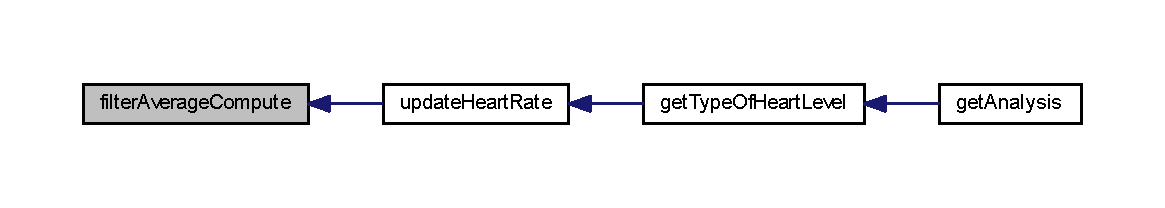
\includegraphics[width=350pt]{filter__math__pincinato_8h_a63b52e2d6e8763a3cb94cd22bde95731_icgraph}
\end{center}
\end{figure}
\mbox{\Hypertarget{filter__math__pincinato_8h_a27ddcf224a294fc542ec5484c6b890bb}\label{filter__math__pincinato_8h_a27ddcf224a294fc542ec5484c6b890bb}} 
\index{filter\+\_\+math\+\_\+pincinato.\+h@{filter\+\_\+math\+\_\+pincinato.\+h}!filter\+Biquads\+Compute@{filter\+Biquads\+Compute}}
\index{filter\+Biquads\+Compute@{filter\+Biquads\+Compute}!filter\+\_\+math\+\_\+pincinato.\+h@{filter\+\_\+math\+\_\+pincinato.\+h}}
\subsubsection{\texorpdfstring{filter\+Biquads\+Compute()}{filterBiquadsCompute()}}
{\footnotesize\ttfamily float filter\+Biquads\+Compute (\begin{DoxyParamCaption}\item[{\mbox{\hyperlink{filter__math__pincinato_8h_a431282902bc1cfeb168d1acf574331bb}{Biquads\+Filter}} $\ast$}]{filter,  }\item[{uint32\+\_\+t}]{value }\end{DoxyParamCaption})}



filter\+Biquads\+Compute Include the value in the filter and compute the filter operation 


\begin{DoxyParams}{Parameters}
{\em filter} & Biquads filter pointer in which the operation will take place. \\
\hline
{\em value} & uin32\+\_\+t value to be add in the filter \\
\hline
\end{DoxyParams}
\begin{DoxyReturn}{Returns}
float with the last result of the filter 
\end{DoxyReturn}


Definition at line 56 of file filter\+\_\+math\+\_\+pincinato.\+c.

\mbox{\Hypertarget{filter__math__pincinato_8h_ae7f97bd805fd61dd0a6bf31e92160672}\label{filter__math__pincinato_8h_ae7f97bd805fd61dd0a6bf31e92160672}} 
\index{filter\+\_\+math\+\_\+pincinato.\+h@{filter\+\_\+math\+\_\+pincinato.\+h}!init\+Average\+Filter@{init\+Average\+Filter}}
\index{init\+Average\+Filter@{init\+Average\+Filter}!filter\+\_\+math\+\_\+pincinato.\+h@{filter\+\_\+math\+\_\+pincinato.\+h}}
\subsubsection{\texorpdfstring{init\+Average\+Filter()}{initAverageFilter()}}
{\footnotesize\ttfamily void init\+Average\+Filter (\begin{DoxyParamCaption}\item[{\mbox{\hyperlink{filter__math__pincinato_8h_a05751bcbb0782121ff05ae3b7fc37dac}{Average\+Filter}} $\ast$}]{filter,  }\item[{float $\ast$}]{d\+\_\+data,  }\item[{int}]{size\+Buffer }\end{DoxyParamCaption})}



init\+Average\+Filter init filter parameters and pointer to respective data 


\begin{DoxyParams}{Parameters}
{\em filter} & pointer to the filter that will be initialized \\
\hline
{\em d\+\_\+data} & float $\ast$ to the buffer that contains the filter values \\
\hline
{\em size\+Buffer} & size of the d\+\_\+data \\
\hline
\end{DoxyParams}


Definition at line 70 of file filter\+\_\+math\+\_\+pincinato.\+c.

Here is the caller graph for this function\+:\nopagebreak
\begin{figure}[H]
\begin{center}
\leavevmode
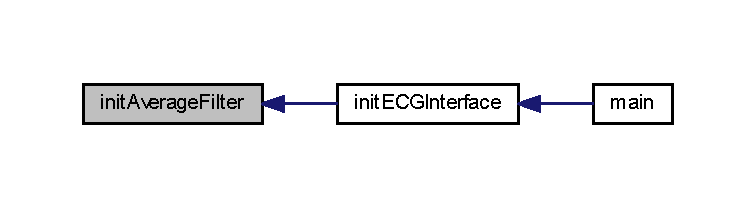
\includegraphics[width=350pt]{filter__math__pincinato_8h_ae7f97bd805fd61dd0a6bf31e92160672_icgraph}
\end{center}
\end{figure}
\mbox{\Hypertarget{filter__math__pincinato_8h_a1e56653839d2baf5ac7f9f2c315e0d3f}\label{filter__math__pincinato_8h_a1e56653839d2baf5ac7f9f2c315e0d3f}} 
\index{filter\+\_\+math\+\_\+pincinato.\+h@{filter\+\_\+math\+\_\+pincinato.\+h}!init\+Biquads\+Filter@{init\+Biquads\+Filter}}
\index{init\+Biquads\+Filter@{init\+Biquads\+Filter}!filter\+\_\+math\+\_\+pincinato.\+h@{filter\+\_\+math\+\_\+pincinato.\+h}}
\subsubsection{\texorpdfstring{init\+Biquads\+Filter()}{initBiquadsFilter()}}
{\footnotesize\ttfamily void init\+Biquads\+Filter (\begin{DoxyParamCaption}\item[{\mbox{\hyperlink{filter__math__pincinato_8h_a431282902bc1cfeb168d1acf574331bb}{Biquads\+Filter}} $\ast$}]{filter,  }\item[{float $\ast$}]{d\+\_\+data,  }\item[{int}]{size\+Buffer,  }\item[{float}]{Acoef\mbox{[}$\,$\mbox{]},  }\item[{float}]{Bcoef\mbox{[}$\,$\mbox{]} }\end{DoxyParamCaption})}



init\+Biquads\+Filter init filter parameters and pointer to respective data 


\begin{DoxyParams}{Parameters}
{\em filter} & Biquads\+Filter pointer to the filter that will be initialized \\
\hline
{\em d\+\_\+data} & float $\ast$ to the buffer that contains the filter values \\
\hline
{\em size\+Buffer} & size of the d\+\_\+data \\
\hline
{\em Acoef} & A Coefficient of the filter \\
\hline
{\em Bcoef} & B Coefficient of the filter \\
\hline
\end{DoxyParams}


Definition at line 32 of file filter\+\_\+math\+\_\+pincinato.\+c.

Here is the caller graph for this function\+:\nopagebreak
\begin{figure}[H]
\begin{center}
\leavevmode
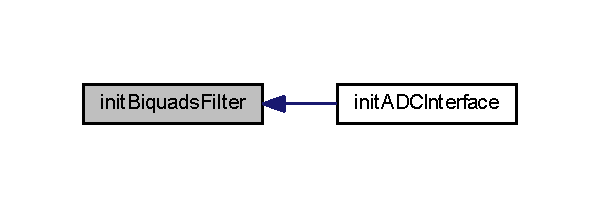
\includegraphics[width=288pt]{filter__math__pincinato_8h_a1e56653839d2baf5ac7f9f2c315e0d3f_icgraph}
\end{center}
\end{figure}
\mbox{\Hypertarget{filter__math__pincinato_8h_a5c31ca586593b15d003e69b87986d9ec}\label{filter__math__pincinato_8h_a5c31ca586593b15d003e69b87986d9ec}} 
\index{filter\+\_\+math\+\_\+pincinato.\+h@{filter\+\_\+math\+\_\+pincinato.\+h}!init\+Integration@{init\+Integration}}
\index{init\+Integration@{init\+Integration}!filter\+\_\+math\+\_\+pincinato.\+h@{filter\+\_\+math\+\_\+pincinato.\+h}}
\subsubsection{\texorpdfstring{init\+Integration()}{initIntegration()}}
{\footnotesize\ttfamily void init\+Integration (\begin{DoxyParamCaption}\item[{\mbox{\hyperlink{filter__math__pincinato_8h_a614628710e855bdeb4949c83265e87e6}{Integration\+Data}} $\ast$}]{integration,  }\item[{float $\ast$}]{d\+\_\+data,  }\item[{int}]{size\+Buffer,  }\item[{float}]{time }\end{DoxyParamCaption})}



init\+Integration initializes the Integration\+Data parameters and pointer to respective data 


\begin{DoxyParams}{Parameters}
{\em integration} & Integration\+Data pointer to the filter that will be initialized \\
\hline
{\em d\+\_\+data} & float $\ast$ to the buffer that contains the filter values \\
\hline
{\em size\+Buffer} & size of the d\+\_\+data \\
\hline
{\em time} & sets time of integration \\
\hline
\end{DoxyParams}


Definition at line 96 of file filter\+\_\+math\+\_\+pincinato.\+c.

Here is the caller graph for this function\+:\nopagebreak
\begin{figure}[H]
\begin{center}
\leavevmode
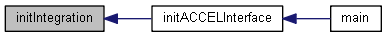
\includegraphics[width=350pt]{filter__math__pincinato_8h_a5c31ca586593b15d003e69b87986d9ec_icgraph}
\end{center}
\end{figure}
\mbox{\Hypertarget{filter__math__pincinato_8h_a59bc40beff6775ed45d464b5d9d1870a}\label{filter__math__pincinato_8h_a59bc40beff6775ed45d464b5d9d1870a}} 
\index{filter\+\_\+math\+\_\+pincinato.\+h@{filter\+\_\+math\+\_\+pincinato.\+h}!integration\+Compute@{integration\+Compute}}
\index{integration\+Compute@{integration\+Compute}!filter\+\_\+math\+\_\+pincinato.\+h@{filter\+\_\+math\+\_\+pincinato.\+h}}
\subsubsection{\texorpdfstring{integration\+Compute()}{integrationCompute()}}
{\footnotesize\ttfamily float integration\+Compute (\begin{DoxyParamCaption}\item[{\mbox{\hyperlink{filter__math__pincinato_8h_a614628710e855bdeb4949c83265e87e6}{Integration\+Data}} $\ast$}]{integral,  }\item[{float}]{n }\end{DoxyParamCaption})}



integration\+Compute include the value in the integration and compute the integration 


\begin{DoxyParams}{Parameters}
{\em integral} & Integartion\+Data to be computed \\
\hline
{\em n} & float value to be add in the integration \\
\hline
\end{DoxyParams}
\begin{DoxyReturn}{Returns}
float value of the last integration 
\end{DoxyReturn}


Definition at line 114 of file filter\+\_\+math\+\_\+pincinato.\+c.

\mbox{\Hypertarget{filter__math__pincinato_8h_ad38cea898eb6470b1635c10c349e2123}\label{filter__math__pincinato_8h_ad38cea898eb6470b1635c10c349e2123}} 
\index{filter\+\_\+math\+\_\+pincinato.\+h@{filter\+\_\+math\+\_\+pincinato.\+h}!integration\+Relative\+Distance@{integration\+Relative\+Distance}}
\index{integration\+Relative\+Distance@{integration\+Relative\+Distance}!filter\+\_\+math\+\_\+pincinato.\+h@{filter\+\_\+math\+\_\+pincinato.\+h}}
\subsubsection{\texorpdfstring{integration\+Relative\+Distance()}{integrationRelativeDistance()}}
{\footnotesize\ttfamily float integration\+Relative\+Distance (\begin{DoxyParamCaption}\item[{\mbox{\hyperlink{filter__math__pincinato_8h_a614628710e855bdeb4949c83265e87e6}{Integration\+Data}} $\ast$}]{integral,  }\item[{float}]{n }\end{DoxyParamCaption})}



integration\+Relative\+Distance Integrates values, regardingless the signal.\+No negative values in the integration. 


\begin{DoxyParams}{Parameters}
{\em integral} & Integration data to be computed \\
\hline
{\em n} & float value to be add in the integration \\
\hline
\end{DoxyParams}
\begin{DoxyReturn}{Returns}
float value of the last relative integration 
\end{DoxyReturn}


Definition at line 127 of file filter\+\_\+math\+\_\+pincinato.\+c.

\mbox{\Hypertarget{filter__math__pincinato_8h_a0943af2024c7552aed64fe01f1bd8e15}\label{filter__math__pincinato_8h_a0943af2024c7552aed64fe01f1bd8e15}} 
\index{filter\+\_\+math\+\_\+pincinato.\+h@{filter\+\_\+math\+\_\+pincinato.\+h}!normalize@{normalize}}
\index{normalize@{normalize}!filter\+\_\+math\+\_\+pincinato.\+h@{filter\+\_\+math\+\_\+pincinato.\+h}}
\subsubsection{\texorpdfstring{normalize()}{normalize()}}
{\footnotesize\ttfamily void normalize (\begin{DoxyParamCaption}\item[{float $\ast$}]{vec,  }\item[{int}]{size }\end{DoxyParamCaption})}



normalize Normalize a arry of float value 


\begin{DoxyParams}{Parameters}
{\em vec} & float $\ast$ to an array, which contains the value to be normalized and after function call, will have the normalized array \\
\hline
{\em size} & int that indicates the size of the array \\
\hline
\end{DoxyParams}


Definition at line 20 of file filter\+\_\+math\+\_\+pincinato.\+c.

Here is the caller graph for this function\+:\nopagebreak
\begin{figure}[H]
\begin{center}
\leavevmode
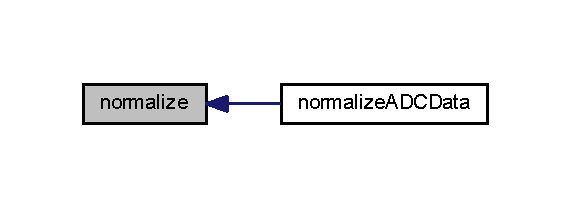
\includegraphics[width=274pt]{filter__math__pincinato_8h_a0943af2024c7552aed64fe01f1bd8e15_icgraph}
\end{center}
\end{figure}

\hypertarget{interface___a_c_c_e_l__pincinato_8h}{}\section{Library/\+Library/inc/interface\+\_\+\+A\+C\+C\+E\+L\+\_\+pincinato.h File Reference}
\label{interface___a_c_c_e_l__pincinato_8h}\index{Library/\+Library/inc/interface\+\_\+\+A\+C\+C\+E\+L\+\_\+pincinato.\+h@{Library/\+Library/inc/interface\+\_\+\+A\+C\+C\+E\+L\+\_\+pincinato.\+h}}
{\ttfamily \#include $<$stdbool.\+h$>$}\newline
{\ttfamily \#include $<$stdint.\+h$>$}\newline
{\ttfamily \#include \char`\"{}i2c.\+h\char`\"{}}\newline
{\ttfamily \#include \char`\"{}tim.\+h\char`\"{}}\newline
{\ttfamily \#include \char`\"{}math.\+h\char`\"{}}\newline
{\ttfamily \#include \char`\"{}filter\+\_\+math\+\_\+pincinato.\+h\char`\"{}}\newline
Include dependency graph for interface\+\_\+\+A\+C\+C\+E\+L\+\_\+pincinato.\+h\+:\nopagebreak
\begin{figure}[H]
\begin{center}
\leavevmode
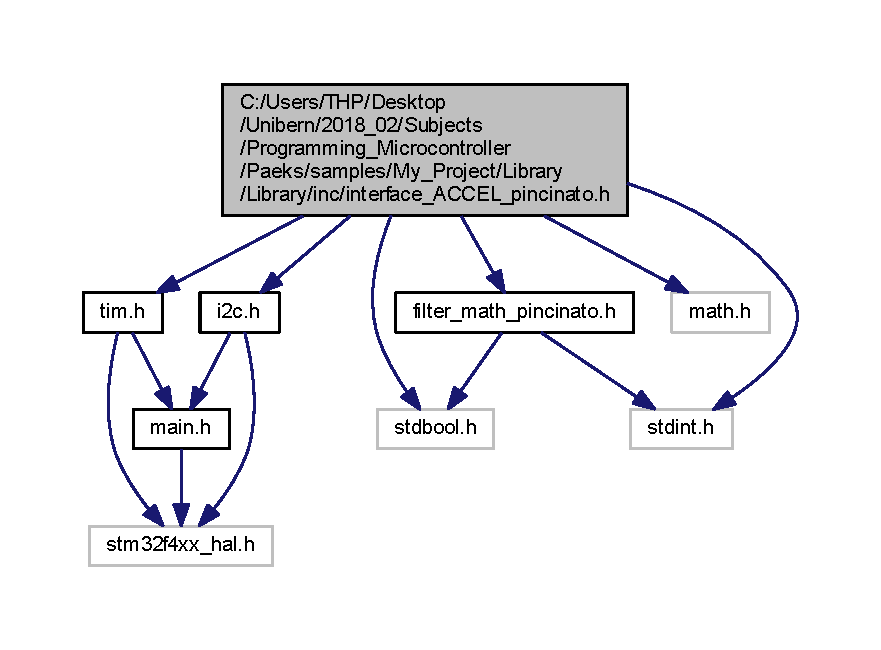
\includegraphics[width=350pt]{interface___a_c_c_e_l__pincinato_8h__incl}
\end{center}
\end{figure}
This graph shows which files directly or indirectly include this file\+:\nopagebreak
\begin{figure}[H]
\begin{center}
\leavevmode
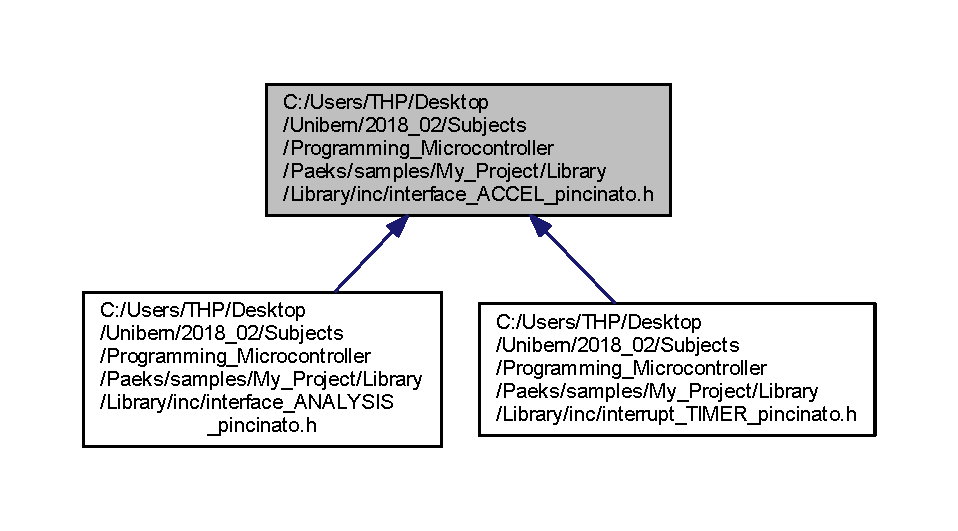
\includegraphics[width=350pt]{interface___a_c_c_e_l__pincinato_8h__dep__incl}
\end{center}
\end{figure}
\subsection*{Data Structures}
\begin{DoxyCompactItemize}
\item 
struct \mbox{\hyperlink{struct_process_data__}{Process\+Data\+\_\+}}
\end{DoxyCompactItemize}
\subsection*{Macros}
\begin{DoxyCompactItemize}
\item 
\#define \mbox{\hyperlink{interface___a_c_c_e_l__pincinato_8h_add97d4e095476a27ddf936822b5f1bbd}{S\+T\+A\+T\+U\+S\+R\+E\+G\+I\+S\+T\+ER}}~0x07
\item 
\#define \mbox{\hyperlink{interface___a_c_c_e_l__pincinato_8h_a1259253323ae1af705b09cc15484d74d}{acell\+Slave\+Adress}}~0x98
\item 
\#define \mbox{\hyperlink{interface___a_c_c_e_l__pincinato_8h_a4a8cad9c6c0df25374c554932af374a2}{accel\+Xout\+Register}}~0x00
\item 
\#define \mbox{\hyperlink{interface___a_c_c_e_l__pincinato_8h_affea857ec7b16c7bd0728c0b8ec78203}{accel\+Yout\+Register}}~0x01
\item 
\#define \mbox{\hyperlink{interface___a_c_c_e_l__pincinato_8h_a6d2b9964d414acbd41bb90d145e0b8d1}{accel\+Zout\+Register}}~0x02
\item 
\#define \mbox{\hyperlink{interface___a_c_c_e_l__pincinato_8h_a47e1d4b27da196f1713508cebac4fd13}{T\+I\+M\+E\+R\+\_\+\+A\+C\+C\+EL}}~\mbox{\hyperlink{tim_8c_aac3d2c59ee0e3bbae1b99529a154eb62}{htim3}}
\item 
\#define \mbox{\hyperlink{interface___a_c_c_e_l__pincinato_8h_a71309642eee768ac00bf3ea62c2b653e}{A\+C\+C\+E\+L\+E\+R\+O\+M\+E\+T\+ER}}~\mbox{\hyperlink{i2c_8c_af7b2c26e44dadaaa798a5c3d82914ba7}{hi2c1}}
\item 
\#define \mbox{\hyperlink{interface___a_c_c_e_l__pincinato_8h_af704f1402c3ac42c867882facf46fc66}{filter\+Item\+Count}}~300
\item 
\#define \mbox{\hyperlink{interface___a_c_c_e_l__pincinato_8h_aeee7ebe36cd3653f48821e6d0da7029d}{integration\+Length}}~100
\item 
\#define \mbox{\hyperlink{interface___a_c_c_e_l__pincinato_8h_a60657962b4e3451455a700693438a26c}{accel\+\_\+\+Category}}~uint8\+\_\+t
\item 
\#define \mbox{\hyperlink{interface___a_c_c_e_l__pincinato_8h_a6270091624318e6aec1026f5f820eaa5}{Category\+\_\+\+H\+I\+GH}}~0xaa
\item 
\#define \mbox{\hyperlink{interface___a_c_c_e_l__pincinato_8h_abcae2af71f22699fa680ddd77be4a515}{Category\+\_\+\+M\+E\+D\+I\+UM}}~0xc0
\item 
\#define \mbox{\hyperlink{interface___a_c_c_e_l__pincinato_8h_acf8b70ab08d45393f6e180920c8bd316}{Category\+\_\+\+L\+OW}}~0x0f
\end{DoxyCompactItemize}
\subsection*{Typedefs}
\begin{DoxyCompactItemize}
\item 
typedef struct \mbox{\hyperlink{struct_process_data__}{Process\+Data\+\_\+}} \mbox{\hyperlink{interface___a_c_c_e_l__pincinato_8h_ab3426c9b59cc17523b6544ee81921b8e}{Process\+Data}}
\end{DoxyCompactItemize}
\subsection*{Functions}
\begin{DoxyCompactItemize}
\item 
void \mbox{\hyperlink{interface___a_c_c_e_l__pincinato_8h_a6820ad75e400340401ebaad4316bdd37}{init\+A\+C\+C\+E\+L\+Interface}} (void)
\begin{DoxyCompactList}\small\item\em init\+A\+C\+C\+E\+L\+Interface Initialize interface, initialize filter, intregation\+Data, and I2C \end{DoxyCompactList}\item 
void \mbox{\hyperlink{interface___a_c_c_e_l__pincinato_8h_aa4357f6d1cf423e55671a0378d3c324e}{start\+A\+C\+C\+E\+L\+Interface}} (void)
\begin{DoxyCompactList}\small\item\em start\+A\+C\+C\+E\+L\+Interface Start interruption time and makes a callibration. \end{DoxyCompactList}\item 
void \mbox{\hyperlink{interface___a_c_c_e_l__pincinato_8h_ada1c73bd592f8c58ce134ada893630e5}{stop\+A\+C\+C\+E\+L\+Interface}} (void)
\begin{DoxyCompactList}\small\item\em stop\+A\+C\+C\+E\+L\+Interface Stop timer interruption \end{DoxyCompactList}\item 
bool \mbox{\hyperlink{interface___a_c_c_e_l__pincinato_8h_aeb17d34699a1c69f8f8dbcdb910e7122}{get\+A\+C\+C\+E\+L\+Category}} (\mbox{\hyperlink{interface___a_c_c_e_l__pincinato_8h_a60657962b4e3451455a700693438a26c}{accel\+\_\+\+Category}} $\ast$value\+Destination)
\item 
bool \mbox{\hyperlink{interface___a_c_c_e_l__pincinato_8h_a3026461e79c24f98e2ad7d3e16399881}{get\+Distance}} (double $\ast$value\+Destination)
\begin{DoxyCompactList}\small\item\em get\+Distance read distance and clear integation \end{DoxyCompactList}\item 
void \mbox{\hyperlink{interface___a_c_c_e_l__pincinato_8h_ad5cd5575c485264b250ac470b0e4b677}{clear\+Data}} (void)
\begin{DoxyCompactList}\small\item\em clear\+Data clear intergation, filter and varibles (set to zero) \end{DoxyCompactList}\item 
float \mbox{\hyperlink{interface___a_c_c_e_l__pincinato_8h_a2af23b2f79bc849201c4f93bb81ca11d}{value\+ToG}} (uint8\+\_\+t value)
\begin{DoxyCompactList}\small\item\em value\+ToG Converts the value of sensor to g value \end{DoxyCompactList}\item 
float \mbox{\hyperlink{interface___a_c_c_e_l__pincinato_8h_a0b85de387060dc919fccc86910164462}{get\+A\+C\+C\+E\+LX}} (void)
\begin{DoxyCompactList}\small\item\em get\+A\+C\+C\+E\+LX get the value of the last value of accelometer in X. \end{DoxyCompactList}\item 
void \mbox{\hyperlink{interface___a_c_c_e_l__pincinato_8h_a86e8ae59804edca8ccce2cd0df75dba1}{interrupt\+Timer\+A\+C\+C\+E\+L\+Callback}} (void)
\begin{DoxyCompactList}\small\item\em interrupt\+Timer\+A\+C\+C\+E\+L\+Callback Handles interruption of time. Set variable to indicate ready to read. \end{DoxyCompactList}\item 
bool \mbox{\hyperlink{interface___a_c_c_e_l__pincinato_8h_a82a51afce6f33aea9486e6fdad232a0d}{read\+Accel}} (void)
\begin{DoxyCompactList}\small\item\em read\+Accel If a value is valid, it read the last accelometer data, convertes, and in the filter and integration \end{DoxyCompactList}\item 
bool \mbox{\hyperlink{interface___a_c_c_e_l__pincinato_8h_ace9c27270108e9c1e16634800babed8a}{calibrate}} (void)
\begin{DoxyCompactList}\small\item\em calibrate set the value of calibration by doing a fisrt measurement \end{DoxyCompactList}\end{DoxyCompactItemize}


\subsection{Macro Definition Documentation}
\mbox{\Hypertarget{interface___a_c_c_e_l__pincinato_8h_a60657962b4e3451455a700693438a26c}\label{interface___a_c_c_e_l__pincinato_8h_a60657962b4e3451455a700693438a26c}} 
\index{interface\+\_\+\+A\+C\+C\+E\+L\+\_\+pincinato.\+h@{interface\+\_\+\+A\+C\+C\+E\+L\+\_\+pincinato.\+h}!accel\+\_\+\+Category@{accel\+\_\+\+Category}}
\index{accel\+\_\+\+Category@{accel\+\_\+\+Category}!interface\+\_\+\+A\+C\+C\+E\+L\+\_\+pincinato.\+h@{interface\+\_\+\+A\+C\+C\+E\+L\+\_\+pincinato.\+h}}
\subsubsection{\texorpdfstring{accel\+\_\+\+Category}{accel\_Category}}
{\footnotesize\ttfamily \#define accel\+\_\+\+Category~uint8\+\_\+t}



Definition at line 32 of file interface\+\_\+\+A\+C\+C\+E\+L\+\_\+pincinato.\+h.

\mbox{\Hypertarget{interface___a_c_c_e_l__pincinato_8h_a71309642eee768ac00bf3ea62c2b653e}\label{interface___a_c_c_e_l__pincinato_8h_a71309642eee768ac00bf3ea62c2b653e}} 
\index{interface\+\_\+\+A\+C\+C\+E\+L\+\_\+pincinato.\+h@{interface\+\_\+\+A\+C\+C\+E\+L\+\_\+pincinato.\+h}!A\+C\+C\+E\+L\+E\+R\+O\+M\+E\+T\+ER@{A\+C\+C\+E\+L\+E\+R\+O\+M\+E\+T\+ER}}
\index{A\+C\+C\+E\+L\+E\+R\+O\+M\+E\+T\+ER@{A\+C\+C\+E\+L\+E\+R\+O\+M\+E\+T\+ER}!interface\+\_\+\+A\+C\+C\+E\+L\+\_\+pincinato.\+h@{interface\+\_\+\+A\+C\+C\+E\+L\+\_\+pincinato.\+h}}
\subsubsection{\texorpdfstring{A\+C\+C\+E\+L\+E\+R\+O\+M\+E\+T\+ER}{ACCELEROMETER}}
{\footnotesize\ttfamily \#define A\+C\+C\+E\+L\+E\+R\+O\+M\+E\+T\+ER~\mbox{\hyperlink{i2c_8c_af7b2c26e44dadaaa798a5c3d82914ba7}{hi2c1}}}



Definition at line 29 of file interface\+\_\+\+A\+C\+C\+E\+L\+\_\+pincinato.\+h.

\mbox{\Hypertarget{interface___a_c_c_e_l__pincinato_8h_a4a8cad9c6c0df25374c554932af374a2}\label{interface___a_c_c_e_l__pincinato_8h_a4a8cad9c6c0df25374c554932af374a2}} 
\index{interface\+\_\+\+A\+C\+C\+E\+L\+\_\+pincinato.\+h@{interface\+\_\+\+A\+C\+C\+E\+L\+\_\+pincinato.\+h}!accel\+Xout\+Register@{accel\+Xout\+Register}}
\index{accel\+Xout\+Register@{accel\+Xout\+Register}!interface\+\_\+\+A\+C\+C\+E\+L\+\_\+pincinato.\+h@{interface\+\_\+\+A\+C\+C\+E\+L\+\_\+pincinato.\+h}}
\subsubsection{\texorpdfstring{accel\+Xout\+Register}{accelXoutRegister}}
{\footnotesize\ttfamily \#define accel\+Xout\+Register~0x00}



Definition at line 25 of file interface\+\_\+\+A\+C\+C\+E\+L\+\_\+pincinato.\+h.

\mbox{\Hypertarget{interface___a_c_c_e_l__pincinato_8h_affea857ec7b16c7bd0728c0b8ec78203}\label{interface___a_c_c_e_l__pincinato_8h_affea857ec7b16c7bd0728c0b8ec78203}} 
\index{interface\+\_\+\+A\+C\+C\+E\+L\+\_\+pincinato.\+h@{interface\+\_\+\+A\+C\+C\+E\+L\+\_\+pincinato.\+h}!accel\+Yout\+Register@{accel\+Yout\+Register}}
\index{accel\+Yout\+Register@{accel\+Yout\+Register}!interface\+\_\+\+A\+C\+C\+E\+L\+\_\+pincinato.\+h@{interface\+\_\+\+A\+C\+C\+E\+L\+\_\+pincinato.\+h}}
\subsubsection{\texorpdfstring{accel\+Yout\+Register}{accelYoutRegister}}
{\footnotesize\ttfamily \#define accel\+Yout\+Register~0x01}



Definition at line 26 of file interface\+\_\+\+A\+C\+C\+E\+L\+\_\+pincinato.\+h.

\mbox{\Hypertarget{interface___a_c_c_e_l__pincinato_8h_a6d2b9964d414acbd41bb90d145e0b8d1}\label{interface___a_c_c_e_l__pincinato_8h_a6d2b9964d414acbd41bb90d145e0b8d1}} 
\index{interface\+\_\+\+A\+C\+C\+E\+L\+\_\+pincinato.\+h@{interface\+\_\+\+A\+C\+C\+E\+L\+\_\+pincinato.\+h}!accel\+Zout\+Register@{accel\+Zout\+Register}}
\index{accel\+Zout\+Register@{accel\+Zout\+Register}!interface\+\_\+\+A\+C\+C\+E\+L\+\_\+pincinato.\+h@{interface\+\_\+\+A\+C\+C\+E\+L\+\_\+pincinato.\+h}}
\subsubsection{\texorpdfstring{accel\+Zout\+Register}{accelZoutRegister}}
{\footnotesize\ttfamily \#define accel\+Zout\+Register~0x02}



Definition at line 27 of file interface\+\_\+\+A\+C\+C\+E\+L\+\_\+pincinato.\+h.

\mbox{\Hypertarget{interface___a_c_c_e_l__pincinato_8h_a1259253323ae1af705b09cc15484d74d}\label{interface___a_c_c_e_l__pincinato_8h_a1259253323ae1af705b09cc15484d74d}} 
\index{interface\+\_\+\+A\+C\+C\+E\+L\+\_\+pincinato.\+h@{interface\+\_\+\+A\+C\+C\+E\+L\+\_\+pincinato.\+h}!acell\+Slave\+Adress@{acell\+Slave\+Adress}}
\index{acell\+Slave\+Adress@{acell\+Slave\+Adress}!interface\+\_\+\+A\+C\+C\+E\+L\+\_\+pincinato.\+h@{interface\+\_\+\+A\+C\+C\+E\+L\+\_\+pincinato.\+h}}
\subsubsection{\texorpdfstring{acell\+Slave\+Adress}{acellSlaveAdress}}
{\footnotesize\ttfamily \#define acell\+Slave\+Adress~0x98}



Definition at line 24 of file interface\+\_\+\+A\+C\+C\+E\+L\+\_\+pincinato.\+h.

\mbox{\Hypertarget{interface___a_c_c_e_l__pincinato_8h_a6270091624318e6aec1026f5f820eaa5}\label{interface___a_c_c_e_l__pincinato_8h_a6270091624318e6aec1026f5f820eaa5}} 
\index{interface\+\_\+\+A\+C\+C\+E\+L\+\_\+pincinato.\+h@{interface\+\_\+\+A\+C\+C\+E\+L\+\_\+pincinato.\+h}!Category\+\_\+\+H\+I\+GH@{Category\+\_\+\+H\+I\+GH}}
\index{Category\+\_\+\+H\+I\+GH@{Category\+\_\+\+H\+I\+GH}!interface\+\_\+\+A\+C\+C\+E\+L\+\_\+pincinato.\+h@{interface\+\_\+\+A\+C\+C\+E\+L\+\_\+pincinato.\+h}}
\subsubsection{\texorpdfstring{Category\+\_\+\+H\+I\+GH}{Category\_HIGH}}
{\footnotesize\ttfamily \#define Category\+\_\+\+H\+I\+GH~0xaa}



Definition at line 33 of file interface\+\_\+\+A\+C\+C\+E\+L\+\_\+pincinato.\+h.

\mbox{\Hypertarget{interface___a_c_c_e_l__pincinato_8h_acf8b70ab08d45393f6e180920c8bd316}\label{interface___a_c_c_e_l__pincinato_8h_acf8b70ab08d45393f6e180920c8bd316}} 
\index{interface\+\_\+\+A\+C\+C\+E\+L\+\_\+pincinato.\+h@{interface\+\_\+\+A\+C\+C\+E\+L\+\_\+pincinato.\+h}!Category\+\_\+\+L\+OW@{Category\+\_\+\+L\+OW}}
\index{Category\+\_\+\+L\+OW@{Category\+\_\+\+L\+OW}!interface\+\_\+\+A\+C\+C\+E\+L\+\_\+pincinato.\+h@{interface\+\_\+\+A\+C\+C\+E\+L\+\_\+pincinato.\+h}}
\subsubsection{\texorpdfstring{Category\+\_\+\+L\+OW}{Category\_LOW}}
{\footnotesize\ttfamily \#define Category\+\_\+\+L\+OW~0x0f}



Definition at line 35 of file interface\+\_\+\+A\+C\+C\+E\+L\+\_\+pincinato.\+h.

\mbox{\Hypertarget{interface___a_c_c_e_l__pincinato_8h_abcae2af71f22699fa680ddd77be4a515}\label{interface___a_c_c_e_l__pincinato_8h_abcae2af71f22699fa680ddd77be4a515}} 
\index{interface\+\_\+\+A\+C\+C\+E\+L\+\_\+pincinato.\+h@{interface\+\_\+\+A\+C\+C\+E\+L\+\_\+pincinato.\+h}!Category\+\_\+\+M\+E\+D\+I\+UM@{Category\+\_\+\+M\+E\+D\+I\+UM}}
\index{Category\+\_\+\+M\+E\+D\+I\+UM@{Category\+\_\+\+M\+E\+D\+I\+UM}!interface\+\_\+\+A\+C\+C\+E\+L\+\_\+pincinato.\+h@{interface\+\_\+\+A\+C\+C\+E\+L\+\_\+pincinato.\+h}}
\subsubsection{\texorpdfstring{Category\+\_\+\+M\+E\+D\+I\+UM}{Category\_MEDIUM}}
{\footnotesize\ttfamily \#define Category\+\_\+\+M\+E\+D\+I\+UM~0xc0}



Definition at line 34 of file interface\+\_\+\+A\+C\+C\+E\+L\+\_\+pincinato.\+h.

\mbox{\Hypertarget{interface___a_c_c_e_l__pincinato_8h_af704f1402c3ac42c867882facf46fc66}\label{interface___a_c_c_e_l__pincinato_8h_af704f1402c3ac42c867882facf46fc66}} 
\index{interface\+\_\+\+A\+C\+C\+E\+L\+\_\+pincinato.\+h@{interface\+\_\+\+A\+C\+C\+E\+L\+\_\+pincinato.\+h}!filter\+Item\+Count@{filter\+Item\+Count}}
\index{filter\+Item\+Count@{filter\+Item\+Count}!interface\+\_\+\+A\+C\+C\+E\+L\+\_\+pincinato.\+h@{interface\+\_\+\+A\+C\+C\+E\+L\+\_\+pincinato.\+h}}
\subsubsection{\texorpdfstring{filter\+Item\+Count}{filterItemCount}}
{\footnotesize\ttfamily \#define filter\+Item\+Count~300}



Definition at line 30 of file interface\+\_\+\+A\+C\+C\+E\+L\+\_\+pincinato.\+h.

\mbox{\Hypertarget{interface___a_c_c_e_l__pincinato_8h_aeee7ebe36cd3653f48821e6d0da7029d}\label{interface___a_c_c_e_l__pincinato_8h_aeee7ebe36cd3653f48821e6d0da7029d}} 
\index{interface\+\_\+\+A\+C\+C\+E\+L\+\_\+pincinato.\+h@{interface\+\_\+\+A\+C\+C\+E\+L\+\_\+pincinato.\+h}!integration\+Length@{integration\+Length}}
\index{integration\+Length@{integration\+Length}!interface\+\_\+\+A\+C\+C\+E\+L\+\_\+pincinato.\+h@{interface\+\_\+\+A\+C\+C\+E\+L\+\_\+pincinato.\+h}}
\subsubsection{\texorpdfstring{integration\+Length}{integrationLength}}
{\footnotesize\ttfamily \#define integration\+Length~100}



Definition at line 31 of file interface\+\_\+\+A\+C\+C\+E\+L\+\_\+pincinato.\+h.

\mbox{\Hypertarget{interface___a_c_c_e_l__pincinato_8h_add97d4e095476a27ddf936822b5f1bbd}\label{interface___a_c_c_e_l__pincinato_8h_add97d4e095476a27ddf936822b5f1bbd}} 
\index{interface\+\_\+\+A\+C\+C\+E\+L\+\_\+pincinato.\+h@{interface\+\_\+\+A\+C\+C\+E\+L\+\_\+pincinato.\+h}!S\+T\+A\+T\+U\+S\+R\+E\+G\+I\+S\+T\+ER@{S\+T\+A\+T\+U\+S\+R\+E\+G\+I\+S\+T\+ER}}
\index{S\+T\+A\+T\+U\+S\+R\+E\+G\+I\+S\+T\+ER@{S\+T\+A\+T\+U\+S\+R\+E\+G\+I\+S\+T\+ER}!interface\+\_\+\+A\+C\+C\+E\+L\+\_\+pincinato.\+h@{interface\+\_\+\+A\+C\+C\+E\+L\+\_\+pincinato.\+h}}
\subsubsection{\texorpdfstring{S\+T\+A\+T\+U\+S\+R\+E\+G\+I\+S\+T\+ER}{STATUSREGISTER}}
{\footnotesize\ttfamily \#define S\+T\+A\+T\+U\+S\+R\+E\+G\+I\+S\+T\+ER~0x07}



Definition at line 23 of file interface\+\_\+\+A\+C\+C\+E\+L\+\_\+pincinato.\+h.

\mbox{\Hypertarget{interface___a_c_c_e_l__pincinato_8h_a47e1d4b27da196f1713508cebac4fd13}\label{interface___a_c_c_e_l__pincinato_8h_a47e1d4b27da196f1713508cebac4fd13}} 
\index{interface\+\_\+\+A\+C\+C\+E\+L\+\_\+pincinato.\+h@{interface\+\_\+\+A\+C\+C\+E\+L\+\_\+pincinato.\+h}!T\+I\+M\+E\+R\+\_\+\+A\+C\+C\+EL@{T\+I\+M\+E\+R\+\_\+\+A\+C\+C\+EL}}
\index{T\+I\+M\+E\+R\+\_\+\+A\+C\+C\+EL@{T\+I\+M\+E\+R\+\_\+\+A\+C\+C\+EL}!interface\+\_\+\+A\+C\+C\+E\+L\+\_\+pincinato.\+h@{interface\+\_\+\+A\+C\+C\+E\+L\+\_\+pincinato.\+h}}
\subsubsection{\texorpdfstring{T\+I\+M\+E\+R\+\_\+\+A\+C\+C\+EL}{TIMER\_ACCEL}}
{\footnotesize\ttfamily \#define T\+I\+M\+E\+R\+\_\+\+A\+C\+C\+EL~\mbox{\hyperlink{tim_8c_aac3d2c59ee0e3bbae1b99529a154eb62}{htim3}}}



Definition at line 28 of file interface\+\_\+\+A\+C\+C\+E\+L\+\_\+pincinato.\+h.



\subsection{Typedef Documentation}
\mbox{\Hypertarget{interface___a_c_c_e_l__pincinato_8h_ab3426c9b59cc17523b6544ee81921b8e}\label{interface___a_c_c_e_l__pincinato_8h_ab3426c9b59cc17523b6544ee81921b8e}} 
\index{interface\+\_\+\+A\+C\+C\+E\+L\+\_\+pincinato.\+h@{interface\+\_\+\+A\+C\+C\+E\+L\+\_\+pincinato.\+h}!Process\+Data@{Process\+Data}}
\index{Process\+Data@{Process\+Data}!interface\+\_\+\+A\+C\+C\+E\+L\+\_\+pincinato.\+h@{interface\+\_\+\+A\+C\+C\+E\+L\+\_\+pincinato.\+h}}
\subsubsection{\texorpdfstring{Process\+Data}{ProcessData}}
{\footnotesize\ttfamily typedef struct \mbox{\hyperlink{struct_process_data__}{Process\+Data\+\_\+}}  \mbox{\hyperlink{interface___a_c_c_e_l__pincinato_8h_ab3426c9b59cc17523b6544ee81921b8e}{Process\+Data}}}



\subsection{Function Documentation}
\mbox{\Hypertarget{interface___a_c_c_e_l__pincinato_8h_ace9c27270108e9c1e16634800babed8a}\label{interface___a_c_c_e_l__pincinato_8h_ace9c27270108e9c1e16634800babed8a}} 
\index{interface\+\_\+\+A\+C\+C\+E\+L\+\_\+pincinato.\+h@{interface\+\_\+\+A\+C\+C\+E\+L\+\_\+pincinato.\+h}!calibrate@{calibrate}}
\index{calibrate@{calibrate}!interface\+\_\+\+A\+C\+C\+E\+L\+\_\+pincinato.\+h@{interface\+\_\+\+A\+C\+C\+E\+L\+\_\+pincinato.\+h}}
\subsubsection{\texorpdfstring{calibrate()}{calibrate()}}
{\footnotesize\ttfamily bool calibrate (\begin{DoxyParamCaption}\item[{void}]{ }\end{DoxyParamCaption})}



calibrate set the value of calibration by doing a fisrt measurement 

\begin{DoxyReturn}{Returns}
return true if operation was succesfull, otherwise false 
\end{DoxyReturn}


Definition at line 42 of file interface\+\_\+\+A\+C\+C\+E\+L\+\_\+pincinato.\+c.

Here is the call graph for this function\+:\nopagebreak
\begin{figure}[H]
\begin{center}
\leavevmode
\includegraphics[width=303pt]{interface___a_c_c_e_l__pincinato_8h_ace9c27270108e9c1e16634800babed8a_cgraph}
\end{center}
\end{figure}
\mbox{\Hypertarget{interface___a_c_c_e_l__pincinato_8h_ad5cd5575c485264b250ac470b0e4b677}\label{interface___a_c_c_e_l__pincinato_8h_ad5cd5575c485264b250ac470b0e4b677}} 
\index{interface\+\_\+\+A\+C\+C\+E\+L\+\_\+pincinato.\+h@{interface\+\_\+\+A\+C\+C\+E\+L\+\_\+pincinato.\+h}!clear\+Data@{clear\+Data}}
\index{clear\+Data@{clear\+Data}!interface\+\_\+\+A\+C\+C\+E\+L\+\_\+pincinato.\+h@{interface\+\_\+\+A\+C\+C\+E\+L\+\_\+pincinato.\+h}}
\subsubsection{\texorpdfstring{clear\+Data()}{clearData()}}
{\footnotesize\ttfamily void clear\+Data (\begin{DoxyParamCaption}\item[{void}]{ }\end{DoxyParamCaption})}



clear\+Data clear intergation, filter and varibles (set to zero) 



Definition at line 84 of file interface\+\_\+\+A\+C\+C\+E\+L\+\_\+pincinato.\+c.

\mbox{\Hypertarget{interface___a_c_c_e_l__pincinato_8h_aeb17d34699a1c69f8f8dbcdb910e7122}\label{interface___a_c_c_e_l__pincinato_8h_aeb17d34699a1c69f8f8dbcdb910e7122}} 
\index{interface\+\_\+\+A\+C\+C\+E\+L\+\_\+pincinato.\+h@{interface\+\_\+\+A\+C\+C\+E\+L\+\_\+pincinato.\+h}!get\+A\+C\+C\+E\+L\+Category@{get\+A\+C\+C\+E\+L\+Category}}
\index{get\+A\+C\+C\+E\+L\+Category@{get\+A\+C\+C\+E\+L\+Category}!interface\+\_\+\+A\+C\+C\+E\+L\+\_\+pincinato.\+h@{interface\+\_\+\+A\+C\+C\+E\+L\+\_\+pincinato.\+h}}
\subsubsection{\texorpdfstring{get\+A\+C\+C\+E\+L\+Category()}{getACCELCategory()}}
{\footnotesize\ttfamily bool get\+A\+C\+C\+E\+L\+Category (\begin{DoxyParamCaption}\item[{\mbox{\hyperlink{interface___a_c_c_e_l__pincinato_8h_a60657962b4e3451455a700693438a26c}{accel\+\_\+\+Category}} $\ast$}]{value\+Destination }\end{DoxyParamCaption})}



Definition at line 70 of file interface\+\_\+\+A\+C\+C\+E\+L\+\_\+pincinato.\+c.

Here is the call graph for this function\+:\nopagebreak
\begin{figure}[H]
\begin{center}
\leavevmode
\includegraphics[width=350pt]{interface___a_c_c_e_l__pincinato_8h_aeb17d34699a1c69f8f8dbcdb910e7122_cgraph}
\end{center}
\end{figure}
\mbox{\Hypertarget{interface___a_c_c_e_l__pincinato_8h_a0b85de387060dc919fccc86910164462}\label{interface___a_c_c_e_l__pincinato_8h_a0b85de387060dc919fccc86910164462}} 
\index{interface\+\_\+\+A\+C\+C\+E\+L\+\_\+pincinato.\+h@{interface\+\_\+\+A\+C\+C\+E\+L\+\_\+pincinato.\+h}!get\+A\+C\+C\+E\+LX@{get\+A\+C\+C\+E\+LX}}
\index{get\+A\+C\+C\+E\+LX@{get\+A\+C\+C\+E\+LX}!interface\+\_\+\+A\+C\+C\+E\+L\+\_\+pincinato.\+h@{interface\+\_\+\+A\+C\+C\+E\+L\+\_\+pincinato.\+h}}
\subsubsection{\texorpdfstring{get\+A\+C\+C\+E\+L\+X()}{getACCELX()}}
{\footnotesize\ttfamily float get\+A\+C\+C\+E\+LX (\begin{DoxyParamCaption}\item[{void}]{ }\end{DoxyParamCaption})}



get\+A\+C\+C\+E\+LX get the value of the last value of accelometer in X. 

\begin{DoxyReturn}{Returns}
float value in \char`\"{}g\char`\"{} units 
\end{DoxyReturn}


Definition at line 53 of file interface\+\_\+\+A\+C\+C\+E\+L\+\_\+pincinato.\+c.

\mbox{\Hypertarget{interface___a_c_c_e_l__pincinato_8h_a3026461e79c24f98e2ad7d3e16399881}\label{interface___a_c_c_e_l__pincinato_8h_a3026461e79c24f98e2ad7d3e16399881}} 
\index{interface\+\_\+\+A\+C\+C\+E\+L\+\_\+pincinato.\+h@{interface\+\_\+\+A\+C\+C\+E\+L\+\_\+pincinato.\+h}!get\+Distance@{get\+Distance}}
\index{get\+Distance@{get\+Distance}!interface\+\_\+\+A\+C\+C\+E\+L\+\_\+pincinato.\+h@{interface\+\_\+\+A\+C\+C\+E\+L\+\_\+pincinato.\+h}}
\subsubsection{\texorpdfstring{get\+Distance()}{getDistance()}}
{\footnotesize\ttfamily bool get\+Distance (\begin{DoxyParamCaption}\item[{double $\ast$}]{value\+Destination }\end{DoxyParamCaption})}



get\+Distance read distance and clear integation 


\begin{DoxyParams}{Parameters}
{\em value\+Destination} & double pointer that receives the distance \\
\hline
\end{DoxyParams}
\begin{DoxyReturn}{Returns}
true if value was set, othrwise false. 
\end{DoxyReturn}


Definition at line 57 of file interface\+\_\+\+A\+C\+C\+E\+L\+\_\+pincinato.\+c.

Here is the call graph for this function\+:\nopagebreak
\begin{figure}[H]
\begin{center}
\leavevmode
\includegraphics[width=318pt]{interface___a_c_c_e_l__pincinato_8h_a3026461e79c24f98e2ad7d3e16399881_cgraph}
\end{center}
\end{figure}
Here is the caller graph for this function\+:\nopagebreak
\begin{figure}[H]
\begin{center}
\leavevmode
\includegraphics[width=350pt]{interface___a_c_c_e_l__pincinato_8h_a3026461e79c24f98e2ad7d3e16399881_icgraph}
\end{center}
\end{figure}
\mbox{\Hypertarget{interface___a_c_c_e_l__pincinato_8h_a6820ad75e400340401ebaad4316bdd37}\label{interface___a_c_c_e_l__pincinato_8h_a6820ad75e400340401ebaad4316bdd37}} 
\index{interface\+\_\+\+A\+C\+C\+E\+L\+\_\+pincinato.\+h@{interface\+\_\+\+A\+C\+C\+E\+L\+\_\+pincinato.\+h}!init\+A\+C\+C\+E\+L\+Interface@{init\+A\+C\+C\+E\+L\+Interface}}
\index{init\+A\+C\+C\+E\+L\+Interface@{init\+A\+C\+C\+E\+L\+Interface}!interface\+\_\+\+A\+C\+C\+E\+L\+\_\+pincinato.\+h@{interface\+\_\+\+A\+C\+C\+E\+L\+\_\+pincinato.\+h}}
\subsubsection{\texorpdfstring{init\+A\+C\+C\+E\+L\+Interface()}{initACCELInterface()}}
{\footnotesize\ttfamily void init\+A\+C\+C\+E\+L\+Interface (\begin{DoxyParamCaption}\item[{void}]{ }\end{DoxyParamCaption})}



init\+A\+C\+C\+E\+L\+Interface Initialize interface, initialize filter, intregation\+Data, and I2C 



Definition at line 20 of file interface\+\_\+\+A\+C\+C\+E\+L\+\_\+pincinato.\+c.

Here is the call graph for this function\+:\nopagebreak
\begin{figure}[H]
\begin{center}
\leavevmode
\includegraphics[width=288pt]{interface___a_c_c_e_l__pincinato_8h_a6820ad75e400340401ebaad4316bdd37_cgraph}
\end{center}
\end{figure}
Here is the caller graph for this function\+:\nopagebreak
\begin{figure}[H]
\begin{center}
\leavevmode
\includegraphics[width=252pt]{interface___a_c_c_e_l__pincinato_8h_a6820ad75e400340401ebaad4316bdd37_icgraph}
\end{center}
\end{figure}
\mbox{\Hypertarget{interface___a_c_c_e_l__pincinato_8h_a86e8ae59804edca8ccce2cd0df75dba1}\label{interface___a_c_c_e_l__pincinato_8h_a86e8ae59804edca8ccce2cd0df75dba1}} 
\index{interface\+\_\+\+A\+C\+C\+E\+L\+\_\+pincinato.\+h@{interface\+\_\+\+A\+C\+C\+E\+L\+\_\+pincinato.\+h}!interrupt\+Timer\+A\+C\+C\+E\+L\+Callback@{interrupt\+Timer\+A\+C\+C\+E\+L\+Callback}}
\index{interrupt\+Timer\+A\+C\+C\+E\+L\+Callback@{interrupt\+Timer\+A\+C\+C\+E\+L\+Callback}!interface\+\_\+\+A\+C\+C\+E\+L\+\_\+pincinato.\+h@{interface\+\_\+\+A\+C\+C\+E\+L\+\_\+pincinato.\+h}}
\subsubsection{\texorpdfstring{interrupt\+Timer\+A\+C\+C\+E\+L\+Callback()}{interruptTimerACCELCallback()}}
{\footnotesize\ttfamily void interrupt\+Timer\+A\+C\+C\+E\+L\+Callback (\begin{DoxyParamCaption}\item[{void}]{ }\end{DoxyParamCaption})}



interrupt\+Timer\+A\+C\+C\+E\+L\+Callback Handles interruption of time. Set variable to indicate ready to read. 



Definition at line 128 of file interface\+\_\+\+A\+C\+C\+E\+L\+\_\+pincinato.\+c.

Here is the caller graph for this function\+:\nopagebreak
\begin{figure}[H]
\begin{center}
\leavevmode
\includegraphics[width=350pt]{interface___a_c_c_e_l__pincinato_8h_a86e8ae59804edca8ccce2cd0df75dba1_icgraph}
\end{center}
\end{figure}
\mbox{\Hypertarget{interface___a_c_c_e_l__pincinato_8h_a82a51afce6f33aea9486e6fdad232a0d}\label{interface___a_c_c_e_l__pincinato_8h_a82a51afce6f33aea9486e6fdad232a0d}} 
\index{interface\+\_\+\+A\+C\+C\+E\+L\+\_\+pincinato.\+h@{interface\+\_\+\+A\+C\+C\+E\+L\+\_\+pincinato.\+h}!read\+Accel@{read\+Accel}}
\index{read\+Accel@{read\+Accel}!interface\+\_\+\+A\+C\+C\+E\+L\+\_\+pincinato.\+h@{interface\+\_\+\+A\+C\+C\+E\+L\+\_\+pincinato.\+h}}
\subsubsection{\texorpdfstring{read\+Accel()}{readAccel()}}
{\footnotesize\ttfamily bool read\+Accel (\begin{DoxyParamCaption}\item[{void}]{ }\end{DoxyParamCaption})}



read\+Accel If a value is valid, it read the last accelometer data, convertes, and in the filter and integration 

\begin{DoxyReturn}{Returns}
return true if operation was succesfull, otherwise false 
\end{DoxyReturn}


Definition at line 102 of file interface\+\_\+\+A\+C\+C\+E\+L\+\_\+pincinato.\+c.

Here is the caller graph for this function\+:\nopagebreak
\begin{figure}[H]
\begin{center}
\leavevmode
\includegraphics[width=350pt]{interface___a_c_c_e_l__pincinato_8h_a82a51afce6f33aea9486e6fdad232a0d_icgraph}
\end{center}
\end{figure}
\mbox{\Hypertarget{interface___a_c_c_e_l__pincinato_8h_aa4357f6d1cf423e55671a0378d3c324e}\label{interface___a_c_c_e_l__pincinato_8h_aa4357f6d1cf423e55671a0378d3c324e}} 
\index{interface\+\_\+\+A\+C\+C\+E\+L\+\_\+pincinato.\+h@{interface\+\_\+\+A\+C\+C\+E\+L\+\_\+pincinato.\+h}!start\+A\+C\+C\+E\+L\+Interface@{start\+A\+C\+C\+E\+L\+Interface}}
\index{start\+A\+C\+C\+E\+L\+Interface@{start\+A\+C\+C\+E\+L\+Interface}!interface\+\_\+\+A\+C\+C\+E\+L\+\_\+pincinato.\+h@{interface\+\_\+\+A\+C\+C\+E\+L\+\_\+pincinato.\+h}}
\subsubsection{\texorpdfstring{start\+A\+C\+C\+E\+L\+Interface()}{startACCELInterface()}}
{\footnotesize\ttfamily void start\+A\+C\+C\+E\+L\+Interface (\begin{DoxyParamCaption}\item[{void}]{ }\end{DoxyParamCaption})}



start\+A\+C\+C\+E\+L\+Interface Start interruption time and makes a callibration. 



Definition at line 30 of file interface\+\_\+\+A\+C\+C\+E\+L\+\_\+pincinato.\+c.

Here is the caller graph for this function\+:\nopagebreak
\begin{figure}[H]
\begin{center}
\leavevmode
\includegraphics[width=342pt]{interface___a_c_c_e_l__pincinato_8h_aa4357f6d1cf423e55671a0378d3c324e_icgraph}
\end{center}
\end{figure}
\mbox{\Hypertarget{interface___a_c_c_e_l__pincinato_8h_ada1c73bd592f8c58ce134ada893630e5}\label{interface___a_c_c_e_l__pincinato_8h_ada1c73bd592f8c58ce134ada893630e5}} 
\index{interface\+\_\+\+A\+C\+C\+E\+L\+\_\+pincinato.\+h@{interface\+\_\+\+A\+C\+C\+E\+L\+\_\+pincinato.\+h}!stop\+A\+C\+C\+E\+L\+Interface@{stop\+A\+C\+C\+E\+L\+Interface}}
\index{stop\+A\+C\+C\+E\+L\+Interface@{stop\+A\+C\+C\+E\+L\+Interface}!interface\+\_\+\+A\+C\+C\+E\+L\+\_\+pincinato.\+h@{interface\+\_\+\+A\+C\+C\+E\+L\+\_\+pincinato.\+h}}
\subsubsection{\texorpdfstring{stop\+A\+C\+C\+E\+L\+Interface()}{stopACCELInterface()}}
{\footnotesize\ttfamily void stop\+A\+C\+C\+E\+L\+Interface (\begin{DoxyParamCaption}\item[{void}]{ }\end{DoxyParamCaption})}



stop\+A\+C\+C\+E\+L\+Interface Stop timer interruption 



Definition at line 38 of file interface\+\_\+\+A\+C\+C\+E\+L\+\_\+pincinato.\+c.

Here is the caller graph for this function\+:\nopagebreak
\begin{figure}[H]
\begin{center}
\leavevmode
\includegraphics[width=340pt]{interface___a_c_c_e_l__pincinato_8h_ada1c73bd592f8c58ce134ada893630e5_icgraph}
\end{center}
\end{figure}
\mbox{\Hypertarget{interface___a_c_c_e_l__pincinato_8h_a2af23b2f79bc849201c4f93bb81ca11d}\label{interface___a_c_c_e_l__pincinato_8h_a2af23b2f79bc849201c4f93bb81ca11d}} 
\index{interface\+\_\+\+A\+C\+C\+E\+L\+\_\+pincinato.\+h@{interface\+\_\+\+A\+C\+C\+E\+L\+\_\+pincinato.\+h}!value\+ToG@{value\+ToG}}
\index{value\+ToG@{value\+ToG}!interface\+\_\+\+A\+C\+C\+E\+L\+\_\+pincinato.\+h@{interface\+\_\+\+A\+C\+C\+E\+L\+\_\+pincinato.\+h}}
\subsubsection{\texorpdfstring{value\+To\+G()}{valueToG()}}
{\footnotesize\ttfamily float value\+ToG (\begin{DoxyParamCaption}\item[{uint8\+\_\+t}]{value }\end{DoxyParamCaption})}



value\+ToG Converts the value of sensor to g value 


\begin{DoxyParams}{Parameters}
{\em value} & uint8\+\_\+t value that contains the information to be converted \\
\hline
\end{DoxyParams}
\begin{DoxyReturn}{Returns}
float value in g reference 
\end{DoxyReturn}


Definition at line 92 of file interface\+\_\+\+A\+C\+C\+E\+L\+\_\+pincinato.\+c.


\hypertarget{interface___a_d_c__pincinato_8h}{}\section{Library/\+Library/inc/interface\+\_\+\+A\+D\+C\+\_\+pincinato.h File Reference}
\label{interface___a_d_c__pincinato_8h}\index{Library/\+Library/inc/interface\+\_\+\+A\+D\+C\+\_\+pincinato.\+h@{Library/\+Library/inc/interface\+\_\+\+A\+D\+C\+\_\+pincinato.\+h}}
{\ttfamily \#include $<$stdbool.\+h$>$}\newline
{\ttfamily \#include $<$stdint.\+h$>$}\newline
{\ttfamily \#include \char`\"{}adc.\+h\char`\"{}}\newline
{\ttfamily \#include \char`\"{}tim.\+h\char`\"{}}\newline
{\ttfamily \#include \char`\"{}filter\+\_\+math\+\_\+pincinato.\+h\char`\"{}}\newline
Include dependency graph for interface\+\_\+\+A\+D\+C\+\_\+pincinato.\+h\+:\nopagebreak
\begin{figure}[H]
\begin{center}
\leavevmode
\includegraphics[width=350pt]{interface___a_d_c__pincinato_8h__incl}
\end{center}
\end{figure}
This graph shows which files directly or indirectly include this file\+:\nopagebreak
\begin{figure}[H]
\begin{center}
\leavevmode
\includegraphics[width=350pt]{interface___a_d_c__pincinato_8h__dep__incl}
\end{center}
\end{figure}
\subsection*{Data Structures}
\begin{DoxyCompactItemize}
\item 
struct \mbox{\hyperlink{struct_process_data____}{Process\+Data\+\_\+\+\_\+}}
\end{DoxyCompactItemize}
\subsection*{Macros}
\begin{DoxyCompactItemize}
\item 
\#define \mbox{\hyperlink{interface___a_d_c__pincinato_8h_a2ddc9b0b00b7c686d5208fc298aeadb2}{A\+D\+C\+B\+U\+F\+F\+E\+R\+L\+E\+N\+G\+TH}}~800
\item 
\#define \mbox{\hyperlink{interface___a_d_c__pincinato_8h_a295555015d57939bf54b7372373e5c81}{T\+I\+M\+E\+R\+\_\+\+A\+DC}}~\mbox{\hyperlink{tim_8c_acefaeaaa3856ddddae7083b2d220fe4b}{htim5}}
\item 
\#define \mbox{\hyperlink{interface___a_d_c__pincinato_8h_a3cb1c4aa16f6ccb5ce78a1eb772e92d3}{A\+D\+C\+\_\+\+I\+N\+P\+UT}}~\mbox{\hyperlink{stm32f4xx__it_8c_a22b804736f5648d52f639b2647d4ed13}{hadc1}}
\end{DoxyCompactItemize}
\subsection*{Typedefs}
\begin{DoxyCompactItemize}
\item 
typedef struct \mbox{\hyperlink{struct_process_data____}{Process\+Data\+\_\+\+\_\+}} \mbox{\hyperlink{interface___a_d_c__pincinato_8h_ab6662b6cd1bbe98ecf5fe7862aeac573}{\+\_\+\+Process\+Data}}
\end{DoxyCompactItemize}
\subsection*{Functions}
\begin{DoxyCompactItemize}
\item 
void \mbox{\hyperlink{interface___a_d_c__pincinato_8h_ac0efe9596a654400ef8be8720c3138d7}{init\+Filter}} (void)
\begin{DoxyCompactList}\small\item\em init\+Filter clear filters \end{DoxyCompactList}\item 
void \mbox{\hyperlink{interface___a_d_c__pincinato_8h_aed3bcce7592bec2169be4a6ef9f7c73d}{init\+A\+D\+C\+Interface}} (void)
\begin{DoxyCompactList}\small\item\em init\+A\+D\+C\+Interface initializes A\+DC intefac; initializes filter, set A and B Biquads coeff \end{DoxyCompactList}\item 
void \mbox{\hyperlink{interface___a_d_c__pincinato_8h_a7be941a43b4f439c481e71bd6c4efdeb}{start\+A\+D\+C\+Interface}} (void)
\begin{DoxyCompactList}\small\item\em start\+A\+D\+C\+Interface call initfilter() and start interruption timer \end{DoxyCompactList}\item 
void \mbox{\hyperlink{interface___a_d_c__pincinato_8h_a5404ec7b3bbcea85079e7c0c8ff9cbd9}{stop\+A\+D\+C\+Interface}} (void)
\begin{DoxyCompactList}\small\item\em stop\+A\+D\+C\+Interface stop A\+DC and timer interruption \end{DoxyCompactList}\item 
void \mbox{\hyperlink{interface___a_d_c__pincinato_8h_a3600f4f837c16ec2da1f17790e310f25}{interrupt\+Timer\+A\+D\+C\+Callback}} (void)
\begin{DoxyCompactList}\small\item\em interrupt\+Timer\+A\+D\+C\+Callback handle interruption and start A\+DC interruption \end{DoxyCompactList}\item 
bool \mbox{\hyperlink{interface___a_d_c__pincinato_8h_a74cb317cbdd6810ff93997cbe6a881ce}{get\+Ready\+To\+Update}} (void)
\begin{DoxyCompactList}\small\item\em get\+Ready\+To\+Update return the value that indicates if the interface is ready to update \end{DoxyCompactList}\item 
void \mbox{\hyperlink{interface___a_d_c__pincinato_8h_ae7da2b0ec678a1583297f19380546ab4}{set\+Ready\+To\+Update}} (bool value)
\begin{DoxyCompactList}\small\item\em set\+Ready\+To\+Update set the variable ready\+To\+Update \end{DoxyCompactList}\item 
const float $\ast$ \mbox{\hyperlink{interface___a_d_c__pincinato_8h_a6dec733976b8a15c23944c88d2dff910}{get\+A\+D\+C\+Data}} (void)
\begin{DoxyCompactList}\small\item\em get\+A\+D\+C\+Data returns a poitner to the float array of the filtered signal \end{DoxyCompactList}\item 
int \mbox{\hyperlink{interface___a_d_c__pincinato_8h_a298b475ed50e670d32558405967a7436}{get\+A\+D\+C\+Data\+Size}} (void)
\begin{DoxyCompactList}\small\item\em get\+A\+D\+C\+Data\+Size returns the size of the array given by get\+A\+D\+C\+Data \end{DoxyCompactList}\item 
void \mbox{\hyperlink{interface___a_d_c__pincinato_8h_ad4f62ce5e9ded73b93486cec97ecd1dd}{normalize\+A\+D\+C\+Data}} (void)
\begin{DoxyCompactList}\small\item\em normalize\+A\+D\+C\+Data normalize the actual filtered signal \end{DoxyCompactList}\item 
void \mbox{\hyperlink{interface___a_d_c__pincinato_8h_aabea500a29263bf4eeb8228943a75d15}{remove\+A\+D\+C\+Unstable\+Values}} (void)
\begin{DoxyCompactList}\small\item\em remove\+A\+D\+C\+Unstable\+Values removes initial unstable values due to the I\+IR filters. \end{DoxyCompactList}\end{DoxyCompactItemize}


\subsection{Macro Definition Documentation}
\mbox{\Hypertarget{interface___a_d_c__pincinato_8h_a3cb1c4aa16f6ccb5ce78a1eb772e92d3}\label{interface___a_d_c__pincinato_8h_a3cb1c4aa16f6ccb5ce78a1eb772e92d3}} 
\index{interface\+\_\+\+A\+D\+C\+\_\+pincinato.\+h@{interface\+\_\+\+A\+D\+C\+\_\+pincinato.\+h}!A\+D\+C\+\_\+\+I\+N\+P\+UT@{A\+D\+C\+\_\+\+I\+N\+P\+UT}}
\index{A\+D\+C\+\_\+\+I\+N\+P\+UT@{A\+D\+C\+\_\+\+I\+N\+P\+UT}!interface\+\_\+\+A\+D\+C\+\_\+pincinato.\+h@{interface\+\_\+\+A\+D\+C\+\_\+pincinato.\+h}}
\subsubsection{\texorpdfstring{A\+D\+C\+\_\+\+I\+N\+P\+UT}{ADC\_INPUT}}
{\footnotesize\ttfamily \#define A\+D\+C\+\_\+\+I\+N\+P\+UT~\mbox{\hyperlink{stm32f4xx__it_8c_a22b804736f5648d52f639b2647d4ed13}{hadc1}}}



Definition at line 25 of file interface\+\_\+\+A\+D\+C\+\_\+pincinato.\+h.

\mbox{\Hypertarget{interface___a_d_c__pincinato_8h_a2ddc9b0b00b7c686d5208fc298aeadb2}\label{interface___a_d_c__pincinato_8h_a2ddc9b0b00b7c686d5208fc298aeadb2}} 
\index{interface\+\_\+\+A\+D\+C\+\_\+pincinato.\+h@{interface\+\_\+\+A\+D\+C\+\_\+pincinato.\+h}!A\+D\+C\+B\+U\+F\+F\+E\+R\+L\+E\+N\+G\+TH@{A\+D\+C\+B\+U\+F\+F\+E\+R\+L\+E\+N\+G\+TH}}
\index{A\+D\+C\+B\+U\+F\+F\+E\+R\+L\+E\+N\+G\+TH@{A\+D\+C\+B\+U\+F\+F\+E\+R\+L\+E\+N\+G\+TH}!interface\+\_\+\+A\+D\+C\+\_\+pincinato.\+h@{interface\+\_\+\+A\+D\+C\+\_\+pincinato.\+h}}
\subsubsection{\texorpdfstring{A\+D\+C\+B\+U\+F\+F\+E\+R\+L\+E\+N\+G\+TH}{ADCBUFFERLENGTH}}
{\footnotesize\ttfamily \#define A\+D\+C\+B\+U\+F\+F\+E\+R\+L\+E\+N\+G\+TH~800}



Definition at line 22 of file interface\+\_\+\+A\+D\+C\+\_\+pincinato.\+h.

\mbox{\Hypertarget{interface___a_d_c__pincinato_8h_a295555015d57939bf54b7372373e5c81}\label{interface___a_d_c__pincinato_8h_a295555015d57939bf54b7372373e5c81}} 
\index{interface\+\_\+\+A\+D\+C\+\_\+pincinato.\+h@{interface\+\_\+\+A\+D\+C\+\_\+pincinato.\+h}!T\+I\+M\+E\+R\+\_\+\+A\+DC@{T\+I\+M\+E\+R\+\_\+\+A\+DC}}
\index{T\+I\+M\+E\+R\+\_\+\+A\+DC@{T\+I\+M\+E\+R\+\_\+\+A\+DC}!interface\+\_\+\+A\+D\+C\+\_\+pincinato.\+h@{interface\+\_\+\+A\+D\+C\+\_\+pincinato.\+h}}
\subsubsection{\texorpdfstring{T\+I\+M\+E\+R\+\_\+\+A\+DC}{TIMER\_ADC}}
{\footnotesize\ttfamily \#define T\+I\+M\+E\+R\+\_\+\+A\+DC~\mbox{\hyperlink{tim_8c_acefaeaaa3856ddddae7083b2d220fe4b}{htim5}}}



Definition at line 24 of file interface\+\_\+\+A\+D\+C\+\_\+pincinato.\+h.



\subsection{Typedef Documentation}
\mbox{\Hypertarget{interface___a_d_c__pincinato_8h_ab6662b6cd1bbe98ecf5fe7862aeac573}\label{interface___a_d_c__pincinato_8h_ab6662b6cd1bbe98ecf5fe7862aeac573}} 
\index{interface\+\_\+\+A\+D\+C\+\_\+pincinato.\+h@{interface\+\_\+\+A\+D\+C\+\_\+pincinato.\+h}!\+\_\+\+Process\+Data@{\+\_\+\+Process\+Data}}
\index{\+\_\+\+Process\+Data@{\+\_\+\+Process\+Data}!interface\+\_\+\+A\+D\+C\+\_\+pincinato.\+h@{interface\+\_\+\+A\+D\+C\+\_\+pincinato.\+h}}
\subsubsection{\texorpdfstring{\+\_\+\+Process\+Data}{\_ProcessData}}
{\footnotesize\ttfamily typedef struct \mbox{\hyperlink{struct_process_data____}{Process\+Data\+\_\+\+\_\+}}  \mbox{\hyperlink{interface___a_d_c__pincinato_8h_ab6662b6cd1bbe98ecf5fe7862aeac573}{\+\_\+\+Process\+Data}}}



\subsection{Function Documentation}
\mbox{\Hypertarget{interface___a_d_c__pincinato_8h_a6dec733976b8a15c23944c88d2dff910}\label{interface___a_d_c__pincinato_8h_a6dec733976b8a15c23944c88d2dff910}} 
\index{interface\+\_\+\+A\+D\+C\+\_\+pincinato.\+h@{interface\+\_\+\+A\+D\+C\+\_\+pincinato.\+h}!get\+A\+D\+C\+Data@{get\+A\+D\+C\+Data}}
\index{get\+A\+D\+C\+Data@{get\+A\+D\+C\+Data}!interface\+\_\+\+A\+D\+C\+\_\+pincinato.\+h@{interface\+\_\+\+A\+D\+C\+\_\+pincinato.\+h}}
\subsubsection{\texorpdfstring{get\+A\+D\+C\+Data()}{getADCData()}}
{\footnotesize\ttfamily const float$\ast$ get\+A\+D\+C\+Data (\begin{DoxyParamCaption}\item[{void}]{ }\end{DoxyParamCaption})}



get\+A\+D\+C\+Data returns a poitner to the float array of the filtered signal 

\begin{DoxyReturn}{Returns}
pointer to an array of float 
\end{DoxyReturn}


Definition at line 49 of file interface\+\_\+\+A\+D\+C\+\_\+pincinato.\+c.

\mbox{\Hypertarget{interface___a_d_c__pincinato_8h_a298b475ed50e670d32558405967a7436}\label{interface___a_d_c__pincinato_8h_a298b475ed50e670d32558405967a7436}} 
\index{interface\+\_\+\+A\+D\+C\+\_\+pincinato.\+h@{interface\+\_\+\+A\+D\+C\+\_\+pincinato.\+h}!get\+A\+D\+C\+Data\+Size@{get\+A\+D\+C\+Data\+Size}}
\index{get\+A\+D\+C\+Data\+Size@{get\+A\+D\+C\+Data\+Size}!interface\+\_\+\+A\+D\+C\+\_\+pincinato.\+h@{interface\+\_\+\+A\+D\+C\+\_\+pincinato.\+h}}
\subsubsection{\texorpdfstring{get\+A\+D\+C\+Data\+Size()}{getADCDataSize()}}
{\footnotesize\ttfamily int get\+A\+D\+C\+Data\+Size (\begin{DoxyParamCaption}\item[{void}]{ }\end{DoxyParamCaption})}



get\+A\+D\+C\+Data\+Size returns the size of the array given by get\+A\+D\+C\+Data 

\begin{DoxyReturn}{Returns}
int 
\end{DoxyReturn}


Definition at line 54 of file interface\+\_\+\+A\+D\+C\+\_\+pincinato.\+c.

\mbox{\Hypertarget{interface___a_d_c__pincinato_8h_a74cb317cbdd6810ff93997cbe6a881ce}\label{interface___a_d_c__pincinato_8h_a74cb317cbdd6810ff93997cbe6a881ce}} 
\index{interface\+\_\+\+A\+D\+C\+\_\+pincinato.\+h@{interface\+\_\+\+A\+D\+C\+\_\+pincinato.\+h}!get\+Ready\+To\+Update@{get\+Ready\+To\+Update}}
\index{get\+Ready\+To\+Update@{get\+Ready\+To\+Update}!interface\+\_\+\+A\+D\+C\+\_\+pincinato.\+h@{interface\+\_\+\+A\+D\+C\+\_\+pincinato.\+h}}
\subsubsection{\texorpdfstring{get\+Ready\+To\+Update()}{getReadyToUpdate()}}
{\footnotesize\ttfamily bool get\+Ready\+To\+Update (\begin{DoxyParamCaption}\item[{void}]{ }\end{DoxyParamCaption})}



get\+Ready\+To\+Update return the value that indicates if the interface is ready to update 

\begin{DoxyReturn}{Returns}
true if it is ready, otherwise false. 
\end{DoxyReturn}


Definition at line 72 of file interface\+\_\+\+A\+D\+C\+\_\+pincinato.\+c.

Here is the caller graph for this function\+:\nopagebreak
\begin{figure}[H]
\begin{center}
\leavevmode
\includegraphics[width=350pt]{interface___a_d_c__pincinato_8h_a74cb317cbdd6810ff93997cbe6a881ce_icgraph}
\end{center}
\end{figure}
\mbox{\Hypertarget{interface___a_d_c__pincinato_8h_aed3bcce7592bec2169be4a6ef9f7c73d}\label{interface___a_d_c__pincinato_8h_aed3bcce7592bec2169be4a6ef9f7c73d}} 
\index{interface\+\_\+\+A\+D\+C\+\_\+pincinato.\+h@{interface\+\_\+\+A\+D\+C\+\_\+pincinato.\+h}!init\+A\+D\+C\+Interface@{init\+A\+D\+C\+Interface}}
\index{init\+A\+D\+C\+Interface@{init\+A\+D\+C\+Interface}!interface\+\_\+\+A\+D\+C\+\_\+pincinato.\+h@{interface\+\_\+\+A\+D\+C\+\_\+pincinato.\+h}}
\subsubsection{\texorpdfstring{init\+A\+D\+C\+Interface()}{initADCInterface()}}
{\footnotesize\ttfamily void init\+A\+D\+C\+Interface (\begin{DoxyParamCaption}\item[{void}]{ }\end{DoxyParamCaption})}



init\+A\+D\+C\+Interface initializes A\+DC intefac; initializes filter, set A and B Biquads coeff 



Definition at line 23 of file interface\+\_\+\+A\+D\+C\+\_\+pincinato.\+c.

Here is the call graph for this function\+:\nopagebreak
\begin{figure}[H]
\begin{center}
\leavevmode
\includegraphics[width=288pt]{interface___a_d_c__pincinato_8h_aed3bcce7592bec2169be4a6ef9f7c73d_cgraph}
\end{center}
\end{figure}
\mbox{\Hypertarget{interface___a_d_c__pincinato_8h_ac0efe9596a654400ef8be8720c3138d7}\label{interface___a_d_c__pincinato_8h_ac0efe9596a654400ef8be8720c3138d7}} 
\index{interface\+\_\+\+A\+D\+C\+\_\+pincinato.\+h@{interface\+\_\+\+A\+D\+C\+\_\+pincinato.\+h}!init\+Filter@{init\+Filter}}
\index{init\+Filter@{init\+Filter}!interface\+\_\+\+A\+D\+C\+\_\+pincinato.\+h@{interface\+\_\+\+A\+D\+C\+\_\+pincinato.\+h}}
\subsubsection{\texorpdfstring{init\+Filter()}{initFilter()}}
{\footnotesize\ttfamily void init\+Filter (\begin{DoxyParamCaption}\item[{void}]{ }\end{DoxyParamCaption})}



init\+Filter clear filters 



Definition at line 43 of file interface\+\_\+\+A\+D\+C\+\_\+pincinato.\+c.

Here is the caller graph for this function\+:\nopagebreak
\begin{figure}[H]
\begin{center}
\leavevmode
\includegraphics[width=350pt]{interface___a_d_c__pincinato_8h_ac0efe9596a654400ef8be8720c3138d7_icgraph}
\end{center}
\end{figure}
\mbox{\Hypertarget{interface___a_d_c__pincinato_8h_a3600f4f837c16ec2da1f17790e310f25}\label{interface___a_d_c__pincinato_8h_a3600f4f837c16ec2da1f17790e310f25}} 
\index{interface\+\_\+\+A\+D\+C\+\_\+pincinato.\+h@{interface\+\_\+\+A\+D\+C\+\_\+pincinato.\+h}!interrupt\+Timer\+A\+D\+C\+Callback@{interrupt\+Timer\+A\+D\+C\+Callback}}
\index{interrupt\+Timer\+A\+D\+C\+Callback@{interrupt\+Timer\+A\+D\+C\+Callback}!interface\+\_\+\+A\+D\+C\+\_\+pincinato.\+h@{interface\+\_\+\+A\+D\+C\+\_\+pincinato.\+h}}
\subsubsection{\texorpdfstring{interrupt\+Timer\+A\+D\+C\+Callback()}{interruptTimerADCCallback()}}
{\footnotesize\ttfamily void interrupt\+Timer\+A\+D\+C\+Callback (\begin{DoxyParamCaption}\item[{void}]{ }\end{DoxyParamCaption})}



interrupt\+Timer\+A\+D\+C\+Callback handle interruption and start A\+DC interruption 



Definition at line 79 of file interface\+\_\+\+A\+D\+C\+\_\+pincinato.\+c.

Here is the caller graph for this function\+:\nopagebreak
\begin{figure}[H]
\begin{center}
\leavevmode
\includegraphics[width=350pt]{interface___a_d_c__pincinato_8h_a3600f4f837c16ec2da1f17790e310f25_icgraph}
\end{center}
\end{figure}
\mbox{\Hypertarget{interface___a_d_c__pincinato_8h_ad4f62ce5e9ded73b93486cec97ecd1dd}\label{interface___a_d_c__pincinato_8h_ad4f62ce5e9ded73b93486cec97ecd1dd}} 
\index{interface\+\_\+\+A\+D\+C\+\_\+pincinato.\+h@{interface\+\_\+\+A\+D\+C\+\_\+pincinato.\+h}!normalize\+A\+D\+C\+Data@{normalize\+A\+D\+C\+Data}}
\index{normalize\+A\+D\+C\+Data@{normalize\+A\+D\+C\+Data}!interface\+\_\+\+A\+D\+C\+\_\+pincinato.\+h@{interface\+\_\+\+A\+D\+C\+\_\+pincinato.\+h}}
\subsubsection{\texorpdfstring{normalize\+A\+D\+C\+Data()}{normalizeADCData()}}
{\footnotesize\ttfamily void normalize\+A\+D\+C\+Data (\begin{DoxyParamCaption}\item[{void}]{ }\end{DoxyParamCaption})}



normalize\+A\+D\+C\+Data normalize the actual filtered signal 



Definition at line 67 of file interface\+\_\+\+A\+D\+C\+\_\+pincinato.\+c.

Here is the call graph for this function\+:\nopagebreak
\begin{figure}[H]
\begin{center}
\leavevmode
\includegraphics[width=274pt]{interface___a_d_c__pincinato_8h_ad4f62ce5e9ded73b93486cec97ecd1dd_cgraph}
\end{center}
\end{figure}
\mbox{\Hypertarget{interface___a_d_c__pincinato_8h_aabea500a29263bf4eeb8228943a75d15}\label{interface___a_d_c__pincinato_8h_aabea500a29263bf4eeb8228943a75d15}} 
\index{interface\+\_\+\+A\+D\+C\+\_\+pincinato.\+h@{interface\+\_\+\+A\+D\+C\+\_\+pincinato.\+h}!remove\+A\+D\+C\+Unstable\+Values@{remove\+A\+D\+C\+Unstable\+Values}}
\index{remove\+A\+D\+C\+Unstable\+Values@{remove\+A\+D\+C\+Unstable\+Values}!interface\+\_\+\+A\+D\+C\+\_\+pincinato.\+h@{interface\+\_\+\+A\+D\+C\+\_\+pincinato.\+h}}
\subsubsection{\texorpdfstring{remove\+A\+D\+C\+Unstable\+Values()}{removeADCUnstableValues()}}
{\footnotesize\ttfamily void remove\+A\+D\+C\+Unstable\+Values (\begin{DoxyParamCaption}\item[{void}]{ }\end{DoxyParamCaption})}



remove\+A\+D\+C\+Unstable\+Values removes initial unstable values due to the I\+IR filters. 



Definition at line 59 of file interface\+\_\+\+A\+D\+C\+\_\+pincinato.\+c.

\mbox{\Hypertarget{interface___a_d_c__pincinato_8h_ae7da2b0ec678a1583297f19380546ab4}\label{interface___a_d_c__pincinato_8h_ae7da2b0ec678a1583297f19380546ab4}} 
\index{interface\+\_\+\+A\+D\+C\+\_\+pincinato.\+h@{interface\+\_\+\+A\+D\+C\+\_\+pincinato.\+h}!set\+Ready\+To\+Update@{set\+Ready\+To\+Update}}
\index{set\+Ready\+To\+Update@{set\+Ready\+To\+Update}!interface\+\_\+\+A\+D\+C\+\_\+pincinato.\+h@{interface\+\_\+\+A\+D\+C\+\_\+pincinato.\+h}}
\subsubsection{\texorpdfstring{set\+Ready\+To\+Update()}{setReadyToUpdate()}}
{\footnotesize\ttfamily void set\+Ready\+To\+Update (\begin{DoxyParamCaption}\item[{bool}]{value }\end{DoxyParamCaption})}



set\+Ready\+To\+Update set the variable ready\+To\+Update 


\begin{DoxyParams}{Parameters}
{\em value} & bool value that will be attribuated to ready\+To\+Update \\
\hline
\end{DoxyParams}


Definition at line 76 of file interface\+\_\+\+A\+D\+C\+\_\+pincinato.\+c.

\mbox{\Hypertarget{interface___a_d_c__pincinato_8h_a7be941a43b4f439c481e71bd6c4efdeb}\label{interface___a_d_c__pincinato_8h_a7be941a43b4f439c481e71bd6c4efdeb}} 
\index{interface\+\_\+\+A\+D\+C\+\_\+pincinato.\+h@{interface\+\_\+\+A\+D\+C\+\_\+pincinato.\+h}!start\+A\+D\+C\+Interface@{start\+A\+D\+C\+Interface}}
\index{start\+A\+D\+C\+Interface@{start\+A\+D\+C\+Interface}!interface\+\_\+\+A\+D\+C\+\_\+pincinato.\+h@{interface\+\_\+\+A\+D\+C\+\_\+pincinato.\+h}}
\subsubsection{\texorpdfstring{start\+A\+D\+C\+Interface()}{startADCInterface()}}
{\footnotesize\ttfamily void start\+A\+D\+C\+Interface (\begin{DoxyParamCaption}\item[{void}]{ }\end{DoxyParamCaption})}



start\+A\+D\+C\+Interface call initfilter() and start interruption timer 



Definition at line 32 of file interface\+\_\+\+A\+D\+C\+\_\+pincinato.\+c.

Here is the call graph for this function\+:\nopagebreak
\begin{figure}[H]
\begin{center}
\leavevmode
\includegraphics[width=260pt]{interface___a_d_c__pincinato_8h_a7be941a43b4f439c481e71bd6c4efdeb_cgraph}
\end{center}
\end{figure}
Here is the caller graph for this function\+:\nopagebreak
\begin{figure}[H]
\begin{center}
\leavevmode
\includegraphics[width=350pt]{interface___a_d_c__pincinato_8h_a7be941a43b4f439c481e71bd6c4efdeb_icgraph}
\end{center}
\end{figure}
\mbox{\Hypertarget{interface___a_d_c__pincinato_8h_a5404ec7b3bbcea85079e7c0c8ff9cbd9}\label{interface___a_d_c__pincinato_8h_a5404ec7b3bbcea85079e7c0c8ff9cbd9}} 
\index{interface\+\_\+\+A\+D\+C\+\_\+pincinato.\+h@{interface\+\_\+\+A\+D\+C\+\_\+pincinato.\+h}!stop\+A\+D\+C\+Interface@{stop\+A\+D\+C\+Interface}}
\index{stop\+A\+D\+C\+Interface@{stop\+A\+D\+C\+Interface}!interface\+\_\+\+A\+D\+C\+\_\+pincinato.\+h@{interface\+\_\+\+A\+D\+C\+\_\+pincinato.\+h}}
\subsubsection{\texorpdfstring{stop\+A\+D\+C\+Interface()}{stopADCInterface()}}
{\footnotesize\ttfamily void stop\+A\+D\+C\+Interface (\begin{DoxyParamCaption}\item[{void}]{ }\end{DoxyParamCaption})}



stop\+A\+D\+C\+Interface stop A\+DC and timer interruption 



Definition at line 38 of file interface\+\_\+\+A\+D\+C\+\_\+pincinato.\+c.

Here is the caller graph for this function\+:\nopagebreak
\begin{figure}[H]
\begin{center}
\leavevmode
\includegraphics[width=350pt]{interface___a_d_c__pincinato_8h_a5404ec7b3bbcea85079e7c0c8ff9cbd9_icgraph}
\end{center}
\end{figure}

\hypertarget{interface___a_n_a_l_y_s_i_s__pincinato_8h}{}\section{Library/\+Library/inc/interface\+\_\+\+A\+N\+A\+L\+Y\+S\+I\+S\+\_\+pincinato.h File Reference}
\label{interface___a_n_a_l_y_s_i_s__pincinato_8h}\index{Library/\+Library/inc/interface\+\_\+\+A\+N\+A\+L\+Y\+S\+I\+S\+\_\+pincinato.\+h@{Library/\+Library/inc/interface\+\_\+\+A\+N\+A\+L\+Y\+S\+I\+S\+\_\+pincinato.\+h}}
{\ttfamily \#include \char`\"{}interface\+\_\+\+E\+C\+G\+\_\+pincinato.\+h\char`\"{}}\newline
{\ttfamily \#include \char`\"{}interface\+\_\+\+A\+C\+C\+E\+L\+\_\+pincinato.\+h\char`\"{}}\newline
{\ttfamily \#include \char`\"{}structs\+\_\+pincinato.\+h\char`\"{}}\newline
Include dependency graph for interface\+\_\+\+A\+N\+A\+L\+Y\+S\+I\+S\+\_\+pincinato.\+h\+:\nopagebreak
\begin{figure}[H]
\begin{center}
\leavevmode
\includegraphics[width=350pt]{interface___a_n_a_l_y_s_i_s__pincinato_8h__incl}
\end{center}
\end{figure}
This graph shows which files directly or indirectly include this file\+:\nopagebreak
\begin{figure}[H]
\begin{center}
\leavevmode
\includegraphics[width=272pt]{interface___a_n_a_l_y_s_i_s__pincinato_8h__dep__incl}
\end{center}
\end{figure}
\subsection*{Data Structures}
\begin{DoxyCompactItemize}
\item 
struct \mbox{\hyperlink{struct_data_buffer}{Data\+Buffer}}
\item 
struct \mbox{\hyperlink{struct_data_buffer__}{Data\+Buffer\+\_\+}}
\item 
struct \mbox{\hyperlink{struct_data_process______}{Data\+Process\+\_\+\+\_\+\+\_\+}}
\end{DoxyCompactItemize}
\subsection*{Macros}
\begin{DoxyCompactItemize}
\item 
\#define \mbox{\hyperlink{interface___a_n_a_l_y_s_i_s__pincinato_8h_a6c0ca8023efe59842a2b2e2f930124cb}{L\+O\+W\+H\+E\+A\+R\+T\+R\+A\+TE}}~0
\item 
\#define \mbox{\hyperlink{interface___a_n_a_l_y_s_i_s__pincinato_8h_af517cfcf2267303b59d25520ab0b38dc}{M\+E\+D\+I\+U\+M\+H\+E\+A\+R\+T\+R\+A\+TE}}~1
\item 
\#define \mbox{\hyperlink{interface___a_n_a_l_y_s_i_s__pincinato_8h_afcca61a5ed06efd4ec7b1a9ae5600ba6}{H\+I\+G\+H\+H\+E\+A\+R\+T\+R\+A\+TE}}~2
\item 
\#define \mbox{\hyperlink{interface___a_n_a_l_y_s_i_s__pincinato_8h_ab539d2729bc388701131d54c761af745}{L\+O\+W\+A\+C\+T\+I\+V\+I\+TY}}~0
\item 
\#define \mbox{\hyperlink{interface___a_n_a_l_y_s_i_s__pincinato_8h_a6d53f71d91d71d3e678a325ff587038c}{M\+E\+D\+I\+U\+M\+A\+C\+T\+I\+V\+I\+TY}}~1
\item 
\#define \mbox{\hyperlink{interface___a_n_a_l_y_s_i_s__pincinato_8h_aa385126b6b3a5c497665ee11df871de6}{H\+I\+G\+H\+A\+C\+T\+I\+V\+I\+TY}}~2
\item 
\#define \mbox{\hyperlink{interface___a_n_a_l_y_s_i_s__pincinato_8h_a3c3573c62ba71a99367ba69784f8723e}{M\+E\+D\+I\+U\+M\+D\+I\+S\+T\+A\+N\+CE}}~1
\item 
\#define \mbox{\hyperlink{interface___a_n_a_l_y_s_i_s__pincinato_8h_ac1ad542e8b168dfc80825e4776f81262}{L\+O\+N\+G\+D\+I\+S\+T\+A\+N\+CE}}~3
\item 
\#define \mbox{\hyperlink{interface___a_n_a_l_y_s_i_s__pincinato_8h_a8d58dfb2133bff91e140c30b2c72ed04}{B\+U\+F\+F\+E\+R\+S\+I\+Z\+E\+A\+N\+A\+L\+Y\+S\+IS}}~5
\item 
\#define \mbox{\hyperlink{interface___a_n_a_l_y_s_i_s__pincinato_8h_a15298070513fb95a1e8c82f64628c9ac}{B\+U\+F\+F\+E\+R\+S\+I\+Z\+E\+A\+B\+N\+O\+R\+M\+A\+L\+I\+T\+I\+ES}}~5
\end{DoxyCompactItemize}
\subsection*{Typedefs}
\begin{DoxyCompactItemize}
\item 
typedef struct \mbox{\hyperlink{struct_data_buffer}{Data\+Buffer}} \mbox{\hyperlink{interface___a_n_a_l_y_s_i_s__pincinato_8h_a3184f2c2dc500ffc383f0a5e8e7f21f0}{my\+Buffer}}
\item 
typedef struct \mbox{\hyperlink{struct_data_buffer__}{Data\+Buffer\+\_\+}} \mbox{\hyperlink{interface___a_n_a_l_y_s_i_s__pincinato_8h_a02b20b214e8ea5dba5c4b81cd4638fc1}{my\+Buffer\+\_\+}}
\item 
typedef struct \mbox{\hyperlink{struct_data_process______}{Data\+Process\+\_\+\+\_\+\+\_\+}} \mbox{\hyperlink{interface___a_n_a_l_y_s_i_s__pincinato_8h_a77b8bfc10caa8f111cbf0c2ea46df1da}{Analysis\+Data\+Process}}
\end{DoxyCompactItemize}
\subsection*{Functions}
\begin{DoxyCompactItemize}
\item 
void \mbox{\hyperlink{interface___a_n_a_l_y_s_i_s__pincinato_8h_a066c88d702a85716f4fe28459ec620aa}{init\+A\+N\+A\+L\+Y\+S\+I\+S\+Interface}} (\mbox{\hyperlink{struct_table}{Table}} $\ast$new\+Table)
\begin{DoxyCompactList}\small\item\em init\+A\+N\+A\+L\+Y\+S\+I\+S\+Interface clear data and set local table \end{DoxyCompactList}\item 
void \mbox{\hyperlink{interface___a_n_a_l_y_s_i_s__pincinato_8h_aa06483b4301e53448aef3c55003b8bde}{start\+A\+N\+A\+L\+Y\+S\+I\+S\+Interface}} (void)
\begin{DoxyCompactList}\small\item\em start\+A\+N\+A\+L\+Y\+S\+I\+S\+Interface clear data and initialize E\+CG and A\+C\+C\+EL interface \end{DoxyCompactList}\item 
void \mbox{\hyperlink{interface___a_n_a_l_y_s_i_s__pincinato_8h_af84609686f3da4bb636a7faa4d2f9204}{stop\+A\+N\+A\+L\+Y\+S\+I\+S\+Interface}} (void)
\begin{DoxyCompactList}\small\item\em stop\+A\+N\+A\+L\+Y\+S\+I\+S\+Interface stop E\+CG and A\+C\+C\+EL interface \end{DoxyCompactList}\item 
void \mbox{\hyperlink{interface___a_n_a_l_y_s_i_s__pincinato_8h_a9736507fb7f0458e69a59134b0edd2e4}{clear\+A\+N\+A\+L\+Y\+S\+I\+S\+Data}} (void)
\begin{DoxyCompactList}\small\item\em clear\+A\+N\+A\+L\+Y\+S\+I\+S\+Data clear all data , including Analysis\+Process \end{DoxyCompactList}\item 
bool \mbox{\hyperlink{interface___a_n_a_l_y_s_i_s__pincinato_8h_a24faadb604f17391d05b528c96a9c433}{get\+Type\+Of\+Activity}} (void)
\begin{DoxyCompactList}\small\item\em get\+Type\+Of\+Activity analyses the value of accel inteface and add the result in the Analysis\+Process \end{DoxyCompactList}\item 
bool \mbox{\hyperlink{interface___a_n_a_l_y_s_i_s__pincinato_8h_a3b17eadb8d65927d28952ff80c6756b4}{get\+Type\+Of\+Heart\+Level}} (void)
\begin{DoxyCompactList}\small\item\em get\+Type\+Of\+Heart\+Level analyses the value of E\+CG inteface and add the result in the Analysis\+Process \end{DoxyCompactList}\item 
bool \mbox{\hyperlink{interface___a_n_a_l_y_s_i_s__pincinato_8h_a43f852ff5bf75bcd4a95d38acd0fa2ec}{get\+Analysis}} (char $\ast$Heart\+Rate\+Classification, char $\ast$Activiy\+Classification, bool $\ast$Abnormal)
\begin{DoxyCompactList}\small\item\em get\+Analysis \end{DoxyCompactList}\item 
void \mbox{\hyperlink{interface___a_n_a_l_y_s_i_s__pincinato_8h_af889f2b019e4434fa7eeb435c0274bb2}{include\+In\+Buffer}} (\mbox{\hyperlink{interface___a_n_a_l_y_s_i_s__pincinato_8h_a3184f2c2dc500ffc383f0a5e8e7f21f0}{my\+Buffer}} $\ast$data, uint32\+\_\+t value\+To\+Include)
\begin{DoxyCompactList}\small\item\em include\+In\+Buffer Include value in the my\+Buffer \end{DoxyCompactList}\item 
uint32\+\_\+t \mbox{\hyperlink{interface___a_n_a_l_y_s_i_s__pincinato_8h_af0a39cf872b07807e0a5fd1eb671addf}{get\+Last\+Included\+In\+Buffer}} (\mbox{\hyperlink{interface___a_n_a_l_y_s_i_s__pincinato_8h_a3184f2c2dc500ffc383f0a5e8e7f21f0}{my\+Buffer}} $\ast$data)
\begin{DoxyCompactList}\small\item\em get\+Last\+Included\+In\+Buffer return last value of a my\+Buffer variable \end{DoxyCompactList}\item 
void \mbox{\hyperlink{interface___a_n_a_l_y_s_i_s__pincinato_8h_a21b240d753d1c7e9f3cfcb09d35eb6fc}{include\+In\+Buffer\+\_\+}} (\mbox{\hyperlink{interface___a_n_a_l_y_s_i_s__pincinato_8h_a02b20b214e8ea5dba5c4b81cd4638fc1}{my\+Buffer\+\_\+}} $\ast$data, bool value\+To\+Include)
\begin{DoxyCompactList}\small\item\em include\+In\+Buffer\+\_\+ Include value in the my\+Buffer\+\_\+ \end{DoxyCompactList}\item 
bool \mbox{\hyperlink{interface___a_n_a_l_y_s_i_s__pincinato_8h_ae03d181b13cf025fb2c4f8c9228a8b97}{is\+Abnormal}} (\mbox{\hyperlink{interface___a_n_a_l_y_s_i_s__pincinato_8h_a02b20b214e8ea5dba5c4b81cd4638fc1}{my\+Buffer\+\_\+}} $\ast$data)
\begin{DoxyCompactList}\small\item\em is\+Abnormal check the my\+Buffer\+\_\+ to verify with the HR is abnormal related with activity \end{DoxyCompactList}\end{DoxyCompactItemize}


\subsection{Macro Definition Documentation}
\mbox{\Hypertarget{interface___a_n_a_l_y_s_i_s__pincinato_8h_a15298070513fb95a1e8c82f64628c9ac}\label{interface___a_n_a_l_y_s_i_s__pincinato_8h_a15298070513fb95a1e8c82f64628c9ac}} 
\index{interface\+\_\+\+A\+N\+A\+L\+Y\+S\+I\+S\+\_\+pincinato.\+h@{interface\+\_\+\+A\+N\+A\+L\+Y\+S\+I\+S\+\_\+pincinato.\+h}!B\+U\+F\+F\+E\+R\+S\+I\+Z\+E\+A\+B\+N\+O\+R\+M\+A\+L\+I\+T\+I\+ES@{B\+U\+F\+F\+E\+R\+S\+I\+Z\+E\+A\+B\+N\+O\+R\+M\+A\+L\+I\+T\+I\+ES}}
\index{B\+U\+F\+F\+E\+R\+S\+I\+Z\+E\+A\+B\+N\+O\+R\+M\+A\+L\+I\+T\+I\+ES@{B\+U\+F\+F\+E\+R\+S\+I\+Z\+E\+A\+B\+N\+O\+R\+M\+A\+L\+I\+T\+I\+ES}!interface\+\_\+\+A\+N\+A\+L\+Y\+S\+I\+S\+\_\+pincinato.\+h@{interface\+\_\+\+A\+N\+A\+L\+Y\+S\+I\+S\+\_\+pincinato.\+h}}
\subsubsection{\texorpdfstring{B\+U\+F\+F\+E\+R\+S\+I\+Z\+E\+A\+B\+N\+O\+R\+M\+A\+L\+I\+T\+I\+ES}{BUFFERSIZEABNORMALITIES}}
{\footnotesize\ttfamily \#define B\+U\+F\+F\+E\+R\+S\+I\+Z\+E\+A\+B\+N\+O\+R\+M\+A\+L\+I\+T\+I\+ES~5}



Definition at line 30 of file interface\+\_\+\+A\+N\+A\+L\+Y\+S\+I\+S\+\_\+pincinato.\+h.

\mbox{\Hypertarget{interface___a_n_a_l_y_s_i_s__pincinato_8h_a8d58dfb2133bff91e140c30b2c72ed04}\label{interface___a_n_a_l_y_s_i_s__pincinato_8h_a8d58dfb2133bff91e140c30b2c72ed04}} 
\index{interface\+\_\+\+A\+N\+A\+L\+Y\+S\+I\+S\+\_\+pincinato.\+h@{interface\+\_\+\+A\+N\+A\+L\+Y\+S\+I\+S\+\_\+pincinato.\+h}!B\+U\+F\+F\+E\+R\+S\+I\+Z\+E\+A\+N\+A\+L\+Y\+S\+IS@{B\+U\+F\+F\+E\+R\+S\+I\+Z\+E\+A\+N\+A\+L\+Y\+S\+IS}}
\index{B\+U\+F\+F\+E\+R\+S\+I\+Z\+E\+A\+N\+A\+L\+Y\+S\+IS@{B\+U\+F\+F\+E\+R\+S\+I\+Z\+E\+A\+N\+A\+L\+Y\+S\+IS}!interface\+\_\+\+A\+N\+A\+L\+Y\+S\+I\+S\+\_\+pincinato.\+h@{interface\+\_\+\+A\+N\+A\+L\+Y\+S\+I\+S\+\_\+pincinato.\+h}}
\subsubsection{\texorpdfstring{B\+U\+F\+F\+E\+R\+S\+I\+Z\+E\+A\+N\+A\+L\+Y\+S\+IS}{BUFFERSIZEANALYSIS}}
{\footnotesize\ttfamily \#define B\+U\+F\+F\+E\+R\+S\+I\+Z\+E\+A\+N\+A\+L\+Y\+S\+IS~5}



Definition at line 29 of file interface\+\_\+\+A\+N\+A\+L\+Y\+S\+I\+S\+\_\+pincinato.\+h.

\mbox{\Hypertarget{interface___a_n_a_l_y_s_i_s__pincinato_8h_aa385126b6b3a5c497665ee11df871de6}\label{interface___a_n_a_l_y_s_i_s__pincinato_8h_aa385126b6b3a5c497665ee11df871de6}} 
\index{interface\+\_\+\+A\+N\+A\+L\+Y\+S\+I\+S\+\_\+pincinato.\+h@{interface\+\_\+\+A\+N\+A\+L\+Y\+S\+I\+S\+\_\+pincinato.\+h}!H\+I\+G\+H\+A\+C\+T\+I\+V\+I\+TY@{H\+I\+G\+H\+A\+C\+T\+I\+V\+I\+TY}}
\index{H\+I\+G\+H\+A\+C\+T\+I\+V\+I\+TY@{H\+I\+G\+H\+A\+C\+T\+I\+V\+I\+TY}!interface\+\_\+\+A\+N\+A\+L\+Y\+S\+I\+S\+\_\+pincinato.\+h@{interface\+\_\+\+A\+N\+A\+L\+Y\+S\+I\+S\+\_\+pincinato.\+h}}
\subsubsection{\texorpdfstring{H\+I\+G\+H\+A\+C\+T\+I\+V\+I\+TY}{HIGHACTIVITY}}
{\footnotesize\ttfamily \#define H\+I\+G\+H\+A\+C\+T\+I\+V\+I\+TY~2}



Definition at line 24 of file interface\+\_\+\+A\+N\+A\+L\+Y\+S\+I\+S\+\_\+pincinato.\+h.

\mbox{\Hypertarget{interface___a_n_a_l_y_s_i_s__pincinato_8h_afcca61a5ed06efd4ec7b1a9ae5600ba6}\label{interface___a_n_a_l_y_s_i_s__pincinato_8h_afcca61a5ed06efd4ec7b1a9ae5600ba6}} 
\index{interface\+\_\+\+A\+N\+A\+L\+Y\+S\+I\+S\+\_\+pincinato.\+h@{interface\+\_\+\+A\+N\+A\+L\+Y\+S\+I\+S\+\_\+pincinato.\+h}!H\+I\+G\+H\+H\+E\+A\+R\+T\+R\+A\+TE@{H\+I\+G\+H\+H\+E\+A\+R\+T\+R\+A\+TE}}
\index{H\+I\+G\+H\+H\+E\+A\+R\+T\+R\+A\+TE@{H\+I\+G\+H\+H\+E\+A\+R\+T\+R\+A\+TE}!interface\+\_\+\+A\+N\+A\+L\+Y\+S\+I\+S\+\_\+pincinato.\+h@{interface\+\_\+\+A\+N\+A\+L\+Y\+S\+I\+S\+\_\+pincinato.\+h}}
\subsubsection{\texorpdfstring{H\+I\+G\+H\+H\+E\+A\+R\+T\+R\+A\+TE}{HIGHHEARTRATE}}
{\footnotesize\ttfamily \#define H\+I\+G\+H\+H\+E\+A\+R\+T\+R\+A\+TE~2}



Definition at line 21 of file interface\+\_\+\+A\+N\+A\+L\+Y\+S\+I\+S\+\_\+pincinato.\+h.

\mbox{\Hypertarget{interface___a_n_a_l_y_s_i_s__pincinato_8h_ac1ad542e8b168dfc80825e4776f81262}\label{interface___a_n_a_l_y_s_i_s__pincinato_8h_ac1ad542e8b168dfc80825e4776f81262}} 
\index{interface\+\_\+\+A\+N\+A\+L\+Y\+S\+I\+S\+\_\+pincinato.\+h@{interface\+\_\+\+A\+N\+A\+L\+Y\+S\+I\+S\+\_\+pincinato.\+h}!L\+O\+N\+G\+D\+I\+S\+T\+A\+N\+CE@{L\+O\+N\+G\+D\+I\+S\+T\+A\+N\+CE}}
\index{L\+O\+N\+G\+D\+I\+S\+T\+A\+N\+CE@{L\+O\+N\+G\+D\+I\+S\+T\+A\+N\+CE}!interface\+\_\+\+A\+N\+A\+L\+Y\+S\+I\+S\+\_\+pincinato.\+h@{interface\+\_\+\+A\+N\+A\+L\+Y\+S\+I\+S\+\_\+pincinato.\+h}}
\subsubsection{\texorpdfstring{L\+O\+N\+G\+D\+I\+S\+T\+A\+N\+CE}{LONGDISTANCE}}
{\footnotesize\ttfamily \#define L\+O\+N\+G\+D\+I\+S\+T\+A\+N\+CE~3}



Definition at line 27 of file interface\+\_\+\+A\+N\+A\+L\+Y\+S\+I\+S\+\_\+pincinato.\+h.

\mbox{\Hypertarget{interface___a_n_a_l_y_s_i_s__pincinato_8h_ab539d2729bc388701131d54c761af745}\label{interface___a_n_a_l_y_s_i_s__pincinato_8h_ab539d2729bc388701131d54c761af745}} 
\index{interface\+\_\+\+A\+N\+A\+L\+Y\+S\+I\+S\+\_\+pincinato.\+h@{interface\+\_\+\+A\+N\+A\+L\+Y\+S\+I\+S\+\_\+pincinato.\+h}!L\+O\+W\+A\+C\+T\+I\+V\+I\+TY@{L\+O\+W\+A\+C\+T\+I\+V\+I\+TY}}
\index{L\+O\+W\+A\+C\+T\+I\+V\+I\+TY@{L\+O\+W\+A\+C\+T\+I\+V\+I\+TY}!interface\+\_\+\+A\+N\+A\+L\+Y\+S\+I\+S\+\_\+pincinato.\+h@{interface\+\_\+\+A\+N\+A\+L\+Y\+S\+I\+S\+\_\+pincinato.\+h}}
\subsubsection{\texorpdfstring{L\+O\+W\+A\+C\+T\+I\+V\+I\+TY}{LOWACTIVITY}}
{\footnotesize\ttfamily \#define L\+O\+W\+A\+C\+T\+I\+V\+I\+TY~0}



Definition at line 22 of file interface\+\_\+\+A\+N\+A\+L\+Y\+S\+I\+S\+\_\+pincinato.\+h.

\mbox{\Hypertarget{interface___a_n_a_l_y_s_i_s__pincinato_8h_a6c0ca8023efe59842a2b2e2f930124cb}\label{interface___a_n_a_l_y_s_i_s__pincinato_8h_a6c0ca8023efe59842a2b2e2f930124cb}} 
\index{interface\+\_\+\+A\+N\+A\+L\+Y\+S\+I\+S\+\_\+pincinato.\+h@{interface\+\_\+\+A\+N\+A\+L\+Y\+S\+I\+S\+\_\+pincinato.\+h}!L\+O\+W\+H\+E\+A\+R\+T\+R\+A\+TE@{L\+O\+W\+H\+E\+A\+R\+T\+R\+A\+TE}}
\index{L\+O\+W\+H\+E\+A\+R\+T\+R\+A\+TE@{L\+O\+W\+H\+E\+A\+R\+T\+R\+A\+TE}!interface\+\_\+\+A\+N\+A\+L\+Y\+S\+I\+S\+\_\+pincinato.\+h@{interface\+\_\+\+A\+N\+A\+L\+Y\+S\+I\+S\+\_\+pincinato.\+h}}
\subsubsection{\texorpdfstring{L\+O\+W\+H\+E\+A\+R\+T\+R\+A\+TE}{LOWHEARTRATE}}
{\footnotesize\ttfamily \#define L\+O\+W\+H\+E\+A\+R\+T\+R\+A\+TE~0}



Definition at line 19 of file interface\+\_\+\+A\+N\+A\+L\+Y\+S\+I\+S\+\_\+pincinato.\+h.

\mbox{\Hypertarget{interface___a_n_a_l_y_s_i_s__pincinato_8h_a6d53f71d91d71d3e678a325ff587038c}\label{interface___a_n_a_l_y_s_i_s__pincinato_8h_a6d53f71d91d71d3e678a325ff587038c}} 
\index{interface\+\_\+\+A\+N\+A\+L\+Y\+S\+I\+S\+\_\+pincinato.\+h@{interface\+\_\+\+A\+N\+A\+L\+Y\+S\+I\+S\+\_\+pincinato.\+h}!M\+E\+D\+I\+U\+M\+A\+C\+T\+I\+V\+I\+TY@{M\+E\+D\+I\+U\+M\+A\+C\+T\+I\+V\+I\+TY}}
\index{M\+E\+D\+I\+U\+M\+A\+C\+T\+I\+V\+I\+TY@{M\+E\+D\+I\+U\+M\+A\+C\+T\+I\+V\+I\+TY}!interface\+\_\+\+A\+N\+A\+L\+Y\+S\+I\+S\+\_\+pincinato.\+h@{interface\+\_\+\+A\+N\+A\+L\+Y\+S\+I\+S\+\_\+pincinato.\+h}}
\subsubsection{\texorpdfstring{M\+E\+D\+I\+U\+M\+A\+C\+T\+I\+V\+I\+TY}{MEDIUMACTIVITY}}
{\footnotesize\ttfamily \#define M\+E\+D\+I\+U\+M\+A\+C\+T\+I\+V\+I\+TY~1}



Definition at line 23 of file interface\+\_\+\+A\+N\+A\+L\+Y\+S\+I\+S\+\_\+pincinato.\+h.

\mbox{\Hypertarget{interface___a_n_a_l_y_s_i_s__pincinato_8h_a3c3573c62ba71a99367ba69784f8723e}\label{interface___a_n_a_l_y_s_i_s__pincinato_8h_a3c3573c62ba71a99367ba69784f8723e}} 
\index{interface\+\_\+\+A\+N\+A\+L\+Y\+S\+I\+S\+\_\+pincinato.\+h@{interface\+\_\+\+A\+N\+A\+L\+Y\+S\+I\+S\+\_\+pincinato.\+h}!M\+E\+D\+I\+U\+M\+D\+I\+S\+T\+A\+N\+CE@{M\+E\+D\+I\+U\+M\+D\+I\+S\+T\+A\+N\+CE}}
\index{M\+E\+D\+I\+U\+M\+D\+I\+S\+T\+A\+N\+CE@{M\+E\+D\+I\+U\+M\+D\+I\+S\+T\+A\+N\+CE}!interface\+\_\+\+A\+N\+A\+L\+Y\+S\+I\+S\+\_\+pincinato.\+h@{interface\+\_\+\+A\+N\+A\+L\+Y\+S\+I\+S\+\_\+pincinato.\+h}}
\subsubsection{\texorpdfstring{M\+E\+D\+I\+U\+M\+D\+I\+S\+T\+A\+N\+CE}{MEDIUMDISTANCE}}
{\footnotesize\ttfamily \#define M\+E\+D\+I\+U\+M\+D\+I\+S\+T\+A\+N\+CE~1}



Definition at line 26 of file interface\+\_\+\+A\+N\+A\+L\+Y\+S\+I\+S\+\_\+pincinato.\+h.

\mbox{\Hypertarget{interface___a_n_a_l_y_s_i_s__pincinato_8h_af517cfcf2267303b59d25520ab0b38dc}\label{interface___a_n_a_l_y_s_i_s__pincinato_8h_af517cfcf2267303b59d25520ab0b38dc}} 
\index{interface\+\_\+\+A\+N\+A\+L\+Y\+S\+I\+S\+\_\+pincinato.\+h@{interface\+\_\+\+A\+N\+A\+L\+Y\+S\+I\+S\+\_\+pincinato.\+h}!M\+E\+D\+I\+U\+M\+H\+E\+A\+R\+T\+R\+A\+TE@{M\+E\+D\+I\+U\+M\+H\+E\+A\+R\+T\+R\+A\+TE}}
\index{M\+E\+D\+I\+U\+M\+H\+E\+A\+R\+T\+R\+A\+TE@{M\+E\+D\+I\+U\+M\+H\+E\+A\+R\+T\+R\+A\+TE}!interface\+\_\+\+A\+N\+A\+L\+Y\+S\+I\+S\+\_\+pincinato.\+h@{interface\+\_\+\+A\+N\+A\+L\+Y\+S\+I\+S\+\_\+pincinato.\+h}}
\subsubsection{\texorpdfstring{M\+E\+D\+I\+U\+M\+H\+E\+A\+R\+T\+R\+A\+TE}{MEDIUMHEARTRATE}}
{\footnotesize\ttfamily \#define M\+E\+D\+I\+U\+M\+H\+E\+A\+R\+T\+R\+A\+TE~1}



Definition at line 20 of file interface\+\_\+\+A\+N\+A\+L\+Y\+S\+I\+S\+\_\+pincinato.\+h.



\subsection{Typedef Documentation}
\mbox{\Hypertarget{interface___a_n_a_l_y_s_i_s__pincinato_8h_a77b8bfc10caa8f111cbf0c2ea46df1da}\label{interface___a_n_a_l_y_s_i_s__pincinato_8h_a77b8bfc10caa8f111cbf0c2ea46df1da}} 
\index{interface\+\_\+\+A\+N\+A\+L\+Y\+S\+I\+S\+\_\+pincinato.\+h@{interface\+\_\+\+A\+N\+A\+L\+Y\+S\+I\+S\+\_\+pincinato.\+h}!Analysis\+Data\+Process@{Analysis\+Data\+Process}}
\index{Analysis\+Data\+Process@{Analysis\+Data\+Process}!interface\+\_\+\+A\+N\+A\+L\+Y\+S\+I\+S\+\_\+pincinato.\+h@{interface\+\_\+\+A\+N\+A\+L\+Y\+S\+I\+S\+\_\+pincinato.\+h}}
\subsubsection{\texorpdfstring{Analysis\+Data\+Process}{AnalysisDataProcess}}
{\footnotesize\ttfamily typedef struct \mbox{\hyperlink{struct_data_process______}{Data\+Process\+\_\+\+\_\+\+\_\+}}  \mbox{\hyperlink{interface___a_n_a_l_y_s_i_s__pincinato_8h_a77b8bfc10caa8f111cbf0c2ea46df1da}{Analysis\+Data\+Process}}}

\mbox{\Hypertarget{interface___a_n_a_l_y_s_i_s__pincinato_8h_a3184f2c2dc500ffc383f0a5e8e7f21f0}\label{interface___a_n_a_l_y_s_i_s__pincinato_8h_a3184f2c2dc500ffc383f0a5e8e7f21f0}} 
\index{interface\+\_\+\+A\+N\+A\+L\+Y\+S\+I\+S\+\_\+pincinato.\+h@{interface\+\_\+\+A\+N\+A\+L\+Y\+S\+I\+S\+\_\+pincinato.\+h}!my\+Buffer@{my\+Buffer}}
\index{my\+Buffer@{my\+Buffer}!interface\+\_\+\+A\+N\+A\+L\+Y\+S\+I\+S\+\_\+pincinato.\+h@{interface\+\_\+\+A\+N\+A\+L\+Y\+S\+I\+S\+\_\+pincinato.\+h}}
\subsubsection{\texorpdfstring{my\+Buffer}{myBuffer}}
{\footnotesize\ttfamily typedef struct \mbox{\hyperlink{struct_data_buffer}{Data\+Buffer}}  \mbox{\hyperlink{interface___a_n_a_l_y_s_i_s__pincinato_8h_a3184f2c2dc500ffc383f0a5e8e7f21f0}{my\+Buffer}}}

\mbox{\Hypertarget{interface___a_n_a_l_y_s_i_s__pincinato_8h_a02b20b214e8ea5dba5c4b81cd4638fc1}\label{interface___a_n_a_l_y_s_i_s__pincinato_8h_a02b20b214e8ea5dba5c4b81cd4638fc1}} 
\index{interface\+\_\+\+A\+N\+A\+L\+Y\+S\+I\+S\+\_\+pincinato.\+h@{interface\+\_\+\+A\+N\+A\+L\+Y\+S\+I\+S\+\_\+pincinato.\+h}!my\+Buffer\+\_\+@{my\+Buffer\+\_\+}}
\index{my\+Buffer\+\_\+@{my\+Buffer\+\_\+}!interface\+\_\+\+A\+N\+A\+L\+Y\+S\+I\+S\+\_\+pincinato.\+h@{interface\+\_\+\+A\+N\+A\+L\+Y\+S\+I\+S\+\_\+pincinato.\+h}}
\subsubsection{\texorpdfstring{my\+Buffer\+\_\+}{myBuffer\_}}
{\footnotesize\ttfamily typedef struct \mbox{\hyperlink{struct_data_buffer__}{Data\+Buffer\+\_\+}}  \mbox{\hyperlink{interface___a_n_a_l_y_s_i_s__pincinato_8h_a02b20b214e8ea5dba5c4b81cd4638fc1}{my\+Buffer\+\_\+}}}



\subsection{Function Documentation}
\mbox{\Hypertarget{interface___a_n_a_l_y_s_i_s__pincinato_8h_a9736507fb7f0458e69a59134b0edd2e4}\label{interface___a_n_a_l_y_s_i_s__pincinato_8h_a9736507fb7f0458e69a59134b0edd2e4}} 
\index{interface\+\_\+\+A\+N\+A\+L\+Y\+S\+I\+S\+\_\+pincinato.\+h@{interface\+\_\+\+A\+N\+A\+L\+Y\+S\+I\+S\+\_\+pincinato.\+h}!clear\+A\+N\+A\+L\+Y\+S\+I\+S\+Data@{clear\+A\+N\+A\+L\+Y\+S\+I\+S\+Data}}
\index{clear\+A\+N\+A\+L\+Y\+S\+I\+S\+Data@{clear\+A\+N\+A\+L\+Y\+S\+I\+S\+Data}!interface\+\_\+\+A\+N\+A\+L\+Y\+S\+I\+S\+\_\+pincinato.\+h@{interface\+\_\+\+A\+N\+A\+L\+Y\+S\+I\+S\+\_\+pincinato.\+h}}
\subsubsection{\texorpdfstring{clear\+A\+N\+A\+L\+Y\+S\+I\+S\+Data()}{clearANALYSISData()}}
{\footnotesize\ttfamily void clear\+A\+N\+A\+L\+Y\+S\+I\+S\+Data (\begin{DoxyParamCaption}\item[{void}]{ }\end{DoxyParamCaption})}



clear\+A\+N\+A\+L\+Y\+S\+I\+S\+Data clear all data , including Analysis\+Process 



Definition at line 26 of file interface\+\_\+\+A\+N\+A\+L\+Y\+S\+I\+S\+\_\+pincinato.\+c.

Here is the caller graph for this function\+:\nopagebreak
\begin{figure}[H]
\begin{center}
\leavevmode
\includegraphics[width=350pt]{interface___a_n_a_l_y_s_i_s__pincinato_8h_a9736507fb7f0458e69a59134b0edd2e4_icgraph}
\end{center}
\end{figure}
\mbox{\Hypertarget{interface___a_n_a_l_y_s_i_s__pincinato_8h_a43f852ff5bf75bcd4a95d38acd0fa2ec}\label{interface___a_n_a_l_y_s_i_s__pincinato_8h_a43f852ff5bf75bcd4a95d38acd0fa2ec}} 
\index{interface\+\_\+\+A\+N\+A\+L\+Y\+S\+I\+S\+\_\+pincinato.\+h@{interface\+\_\+\+A\+N\+A\+L\+Y\+S\+I\+S\+\_\+pincinato.\+h}!get\+Analysis@{get\+Analysis}}
\index{get\+Analysis@{get\+Analysis}!interface\+\_\+\+A\+N\+A\+L\+Y\+S\+I\+S\+\_\+pincinato.\+h@{interface\+\_\+\+A\+N\+A\+L\+Y\+S\+I\+S\+\_\+pincinato.\+h}}
\subsubsection{\texorpdfstring{get\+Analysis()}{getAnalysis()}}
{\footnotesize\ttfamily bool get\+Analysis (\begin{DoxyParamCaption}\item[{char $\ast$}]{Heart\+Rate\+Classification,  }\item[{char $\ast$}]{Activiy\+Classification,  }\item[{bool $\ast$}]{Abnormal }\end{DoxyParamCaption})}



get\+Analysis 


\begin{DoxyParams}{Parameters}
{\em Heart\+Rate\+Classification} & char pointer that recieves the classification of Heart Rate \\
\hline
{\em Activiy\+Classification} & char pointer that recieves the classitication of Heart Rate \\
\hline
{\em Abnormal} & bool pointer that recieves true when a abnormality is observed \\
\hline
\end{DoxyParams}
\begin{DoxyReturn}{Returns}
true if a new analisys was done, false if not. 
\end{DoxyReturn}


Definition at line 83 of file interface\+\_\+\+A\+N\+A\+L\+Y\+S\+I\+S\+\_\+pincinato.\+c.

Here is the call graph for this function\+:\nopagebreak
\begin{figure}[H]
\begin{center}
\leavevmode
\includegraphics[width=350pt]{interface___a_n_a_l_y_s_i_s__pincinato_8h_a43f852ff5bf75bcd4a95d38acd0fa2ec_cgraph}
\end{center}
\end{figure}
\mbox{\Hypertarget{interface___a_n_a_l_y_s_i_s__pincinato_8h_af0a39cf872b07807e0a5fd1eb671addf}\label{interface___a_n_a_l_y_s_i_s__pincinato_8h_af0a39cf872b07807e0a5fd1eb671addf}} 
\index{interface\+\_\+\+A\+N\+A\+L\+Y\+S\+I\+S\+\_\+pincinato.\+h@{interface\+\_\+\+A\+N\+A\+L\+Y\+S\+I\+S\+\_\+pincinato.\+h}!get\+Last\+Included\+In\+Buffer@{get\+Last\+Included\+In\+Buffer}}
\index{get\+Last\+Included\+In\+Buffer@{get\+Last\+Included\+In\+Buffer}!interface\+\_\+\+A\+N\+A\+L\+Y\+S\+I\+S\+\_\+pincinato.\+h@{interface\+\_\+\+A\+N\+A\+L\+Y\+S\+I\+S\+\_\+pincinato.\+h}}
\subsubsection{\texorpdfstring{get\+Last\+Included\+In\+Buffer()}{getLastIncludedInBuffer()}}
{\footnotesize\ttfamily uint32\+\_\+t get\+Last\+Included\+In\+Buffer (\begin{DoxyParamCaption}\item[{\mbox{\hyperlink{interface___a_n_a_l_y_s_i_s__pincinato_8h_a3184f2c2dc500ffc383f0a5e8e7f21f0}{my\+Buffer}} $\ast$}]{data }\end{DoxyParamCaption})}



get\+Last\+Included\+In\+Buffer return last value of a my\+Buffer variable 


\begin{DoxyParams}{Parameters}
{\em data} & my\+Buffer in which the last value will be returned \\
\hline
\end{DoxyParams}
\begin{DoxyReturn}{Returns}
last value of my\+Buffer 
\end{DoxyReturn}


Definition at line 148 of file interface\+\_\+\+A\+N\+A\+L\+Y\+S\+I\+S\+\_\+pincinato.\+c.

\mbox{\Hypertarget{interface___a_n_a_l_y_s_i_s__pincinato_8h_a24faadb604f17391d05b528c96a9c433}\label{interface___a_n_a_l_y_s_i_s__pincinato_8h_a24faadb604f17391d05b528c96a9c433}} 
\index{interface\+\_\+\+A\+N\+A\+L\+Y\+S\+I\+S\+\_\+pincinato.\+h@{interface\+\_\+\+A\+N\+A\+L\+Y\+S\+I\+S\+\_\+pincinato.\+h}!get\+Type\+Of\+Activity@{get\+Type\+Of\+Activity}}
\index{get\+Type\+Of\+Activity@{get\+Type\+Of\+Activity}!interface\+\_\+\+A\+N\+A\+L\+Y\+S\+I\+S\+\_\+pincinato.\+h@{interface\+\_\+\+A\+N\+A\+L\+Y\+S\+I\+S\+\_\+pincinato.\+h}}
\subsubsection{\texorpdfstring{get\+Type\+Of\+Activity()}{getTypeOfActivity()}}
{\footnotesize\ttfamily bool get\+Type\+Of\+Activity (\begin{DoxyParamCaption}\item[{void}]{ }\end{DoxyParamCaption})}



get\+Type\+Of\+Activity analyses the value of accel inteface and add the result in the Analysis\+Process 

\begin{DoxyReturn}{Returns}
true if a new value was added, false if not. 
\end{DoxyReturn}


Definition at line 56 of file interface\+\_\+\+A\+N\+A\+L\+Y\+S\+I\+S\+\_\+pincinato.\+c.

Here is the call graph for this function\+:\nopagebreak
\begin{figure}[H]
\begin{center}
\leavevmode
\includegraphics[width=350pt]{interface___a_n_a_l_y_s_i_s__pincinato_8h_a24faadb604f17391d05b528c96a9c433_cgraph}
\end{center}
\end{figure}
Here is the caller graph for this function\+:\nopagebreak
\begin{figure}[H]
\begin{center}
\leavevmode
\includegraphics[width=276pt]{interface___a_n_a_l_y_s_i_s__pincinato_8h_a24faadb604f17391d05b528c96a9c433_icgraph}
\end{center}
\end{figure}
\mbox{\Hypertarget{interface___a_n_a_l_y_s_i_s__pincinato_8h_a3b17eadb8d65927d28952ff80c6756b4}\label{interface___a_n_a_l_y_s_i_s__pincinato_8h_a3b17eadb8d65927d28952ff80c6756b4}} 
\index{interface\+\_\+\+A\+N\+A\+L\+Y\+S\+I\+S\+\_\+pincinato.\+h@{interface\+\_\+\+A\+N\+A\+L\+Y\+S\+I\+S\+\_\+pincinato.\+h}!get\+Type\+Of\+Heart\+Level@{get\+Type\+Of\+Heart\+Level}}
\index{get\+Type\+Of\+Heart\+Level@{get\+Type\+Of\+Heart\+Level}!interface\+\_\+\+A\+N\+A\+L\+Y\+S\+I\+S\+\_\+pincinato.\+h@{interface\+\_\+\+A\+N\+A\+L\+Y\+S\+I\+S\+\_\+pincinato.\+h}}
\subsubsection{\texorpdfstring{get\+Type\+Of\+Heart\+Level()}{getTypeOfHeartLevel()}}
{\footnotesize\ttfamily bool get\+Type\+Of\+Heart\+Level (\begin{DoxyParamCaption}\item[{void}]{ }\end{DoxyParamCaption})}



get\+Type\+Of\+Heart\+Level analyses the value of E\+CG inteface and add the result in the Analysis\+Process 

\begin{DoxyReturn}{Returns}
true if a new value was added, false if not. 
\end{DoxyReturn}


Definition at line 70 of file interface\+\_\+\+A\+N\+A\+L\+Y\+S\+I\+S\+\_\+pincinato.\+c.

Here is the call graph for this function\+:\nopagebreak
\begin{figure}[H]
\begin{center}
\leavevmode
\includegraphics[width=350pt]{interface___a_n_a_l_y_s_i_s__pincinato_8h_a3b17eadb8d65927d28952ff80c6756b4_cgraph}
\end{center}
\end{figure}
Here is the caller graph for this function\+:\nopagebreak
\begin{figure}[H]
\begin{center}
\leavevmode
\includegraphics[width=290pt]{interface___a_n_a_l_y_s_i_s__pincinato_8h_a3b17eadb8d65927d28952ff80c6756b4_icgraph}
\end{center}
\end{figure}
\mbox{\Hypertarget{interface___a_n_a_l_y_s_i_s__pincinato_8h_af889f2b019e4434fa7eeb435c0274bb2}\label{interface___a_n_a_l_y_s_i_s__pincinato_8h_af889f2b019e4434fa7eeb435c0274bb2}} 
\index{interface\+\_\+\+A\+N\+A\+L\+Y\+S\+I\+S\+\_\+pincinato.\+h@{interface\+\_\+\+A\+N\+A\+L\+Y\+S\+I\+S\+\_\+pincinato.\+h}!include\+In\+Buffer@{include\+In\+Buffer}}
\index{include\+In\+Buffer@{include\+In\+Buffer}!interface\+\_\+\+A\+N\+A\+L\+Y\+S\+I\+S\+\_\+pincinato.\+h@{interface\+\_\+\+A\+N\+A\+L\+Y\+S\+I\+S\+\_\+pincinato.\+h}}
\subsubsection{\texorpdfstring{include\+In\+Buffer()}{includeInBuffer()}}
{\footnotesize\ttfamily void include\+In\+Buffer (\begin{DoxyParamCaption}\item[{\mbox{\hyperlink{interface___a_n_a_l_y_s_i_s__pincinato_8h_a3184f2c2dc500ffc383f0a5e8e7f21f0}{my\+Buffer}} $\ast$}]{data,  }\item[{uint32\+\_\+t}]{value\+To\+Include }\end{DoxyParamCaption})}



include\+In\+Buffer Include value in the my\+Buffer 


\begin{DoxyParams}{Parameters}
{\em data} & my\+Buffer in which a new\+Value will be included \\
\hline
{\em value\+To\+Include} & values to be included \\
\hline
\end{DoxyParams}


Definition at line 126 of file interface\+\_\+\+A\+N\+A\+L\+Y\+S\+I\+S\+\_\+pincinato.\+c.

Here is the caller graph for this function\+:\nopagebreak
\begin{figure}[H]
\begin{center}
\leavevmode
\includegraphics[width=350pt]{interface___a_n_a_l_y_s_i_s__pincinato_8h_af889f2b019e4434fa7eeb435c0274bb2_icgraph}
\end{center}
\end{figure}
\mbox{\Hypertarget{interface___a_n_a_l_y_s_i_s__pincinato_8h_a21b240d753d1c7e9f3cfcb09d35eb6fc}\label{interface___a_n_a_l_y_s_i_s__pincinato_8h_a21b240d753d1c7e9f3cfcb09d35eb6fc}} 
\index{interface\+\_\+\+A\+N\+A\+L\+Y\+S\+I\+S\+\_\+pincinato.\+h@{interface\+\_\+\+A\+N\+A\+L\+Y\+S\+I\+S\+\_\+pincinato.\+h}!include\+In\+Buffer\+\_\+@{include\+In\+Buffer\+\_\+}}
\index{include\+In\+Buffer\+\_\+@{include\+In\+Buffer\+\_\+}!interface\+\_\+\+A\+N\+A\+L\+Y\+S\+I\+S\+\_\+pincinato.\+h@{interface\+\_\+\+A\+N\+A\+L\+Y\+S\+I\+S\+\_\+pincinato.\+h}}
\subsubsection{\texorpdfstring{include\+In\+Buffer\+\_\+()}{includeInBuffer\_()}}
{\footnotesize\ttfamily void include\+In\+Buffer\+\_\+ (\begin{DoxyParamCaption}\item[{\mbox{\hyperlink{interface___a_n_a_l_y_s_i_s__pincinato_8h_a02b20b214e8ea5dba5c4b81cd4638fc1}{my\+Buffer\+\_\+}} $\ast$}]{data,  }\item[{bool}]{value\+To\+Include }\end{DoxyParamCaption})}



include\+In\+Buffer\+\_\+ Include value in the my\+Buffer\+\_\+ 


\begin{DoxyParams}{Parameters}
{\em data} & my\+Buffer\+\_\+ in which a new\+Value will be included \\
\hline
{\em value\+To\+Include} & values to be included \\
\hline
\end{DoxyParams}


Definition at line 138 of file interface\+\_\+\+A\+N\+A\+L\+Y\+S\+I\+S\+\_\+pincinato.\+c.

\mbox{\Hypertarget{interface___a_n_a_l_y_s_i_s__pincinato_8h_a066c88d702a85716f4fe28459ec620aa}\label{interface___a_n_a_l_y_s_i_s__pincinato_8h_a066c88d702a85716f4fe28459ec620aa}} 
\index{interface\+\_\+\+A\+N\+A\+L\+Y\+S\+I\+S\+\_\+pincinato.\+h@{interface\+\_\+\+A\+N\+A\+L\+Y\+S\+I\+S\+\_\+pincinato.\+h}!init\+A\+N\+A\+L\+Y\+S\+I\+S\+Interface@{init\+A\+N\+A\+L\+Y\+S\+I\+S\+Interface}}
\index{init\+A\+N\+A\+L\+Y\+S\+I\+S\+Interface@{init\+A\+N\+A\+L\+Y\+S\+I\+S\+Interface}!interface\+\_\+\+A\+N\+A\+L\+Y\+S\+I\+S\+\_\+pincinato.\+h@{interface\+\_\+\+A\+N\+A\+L\+Y\+S\+I\+S\+\_\+pincinato.\+h}}
\subsubsection{\texorpdfstring{init\+A\+N\+A\+L\+Y\+S\+I\+S\+Interface()}{initANALYSISInterface()}}
{\footnotesize\ttfamily void init\+A\+N\+A\+L\+Y\+S\+I\+S\+Interface (\begin{DoxyParamCaption}\item[{\mbox{\hyperlink{struct_table}{Table}} $\ast$}]{new\+Table }\end{DoxyParamCaption})}



init\+A\+N\+A\+L\+Y\+S\+I\+S\+Interface clear data and set local table 


\begin{DoxyParams}{Parameters}
{\em new\+Table} & new table that will be assigned to local\+Table variable \\
\hline
\end{DoxyParams}


Definition at line 20 of file interface\+\_\+\+A\+N\+A\+L\+Y\+S\+I\+S\+\_\+pincinato.\+c.

Here is the call graph for this function\+:\nopagebreak
\begin{figure}[H]
\begin{center}
\leavevmode
\includegraphics[width=336pt]{interface___a_n_a_l_y_s_i_s__pincinato_8h_a066c88d702a85716f4fe28459ec620aa_cgraph}
\end{center}
\end{figure}
Here is the caller graph for this function\+:\nopagebreak
\begin{figure}[H]
\begin{center}
\leavevmode
\includegraphics[width=268pt]{interface___a_n_a_l_y_s_i_s__pincinato_8h_a066c88d702a85716f4fe28459ec620aa_icgraph}
\end{center}
\end{figure}
\mbox{\Hypertarget{interface___a_n_a_l_y_s_i_s__pincinato_8h_ae03d181b13cf025fb2c4f8c9228a8b97}\label{interface___a_n_a_l_y_s_i_s__pincinato_8h_ae03d181b13cf025fb2c4f8c9228a8b97}} 
\index{interface\+\_\+\+A\+N\+A\+L\+Y\+S\+I\+S\+\_\+pincinato.\+h@{interface\+\_\+\+A\+N\+A\+L\+Y\+S\+I\+S\+\_\+pincinato.\+h}!is\+Abnormal@{is\+Abnormal}}
\index{is\+Abnormal@{is\+Abnormal}!interface\+\_\+\+A\+N\+A\+L\+Y\+S\+I\+S\+\_\+pincinato.\+h@{interface\+\_\+\+A\+N\+A\+L\+Y\+S\+I\+S\+\_\+pincinato.\+h}}
\subsubsection{\texorpdfstring{is\+Abnormal()}{isAbnormal()}}
{\footnotesize\ttfamily bool is\+Abnormal (\begin{DoxyParamCaption}\item[{\mbox{\hyperlink{interface___a_n_a_l_y_s_i_s__pincinato_8h_a02b20b214e8ea5dba5c4b81cd4638fc1}{my\+Buffer\+\_\+}} $\ast$}]{data }\end{DoxyParamCaption})}



is\+Abnormal check the my\+Buffer\+\_\+ to verify with the HR is abnormal related with activity 


\begin{DoxyParams}{Parameters}
{\em data} & my\+Buffer\+\_\+ to be analysed \\
\hline
\end{DoxyParams}
\begin{DoxyReturn}{Returns}
true if all value of the array are abnormal 
\end{DoxyReturn}


Definition at line 160 of file interface\+\_\+\+A\+N\+A\+L\+Y\+S\+I\+S\+\_\+pincinato.\+c.

Here is the call graph for this function\+:\nopagebreak
\begin{figure}[H]
\begin{center}
\leavevmode
\includegraphics[width=315pt]{interface___a_n_a_l_y_s_i_s__pincinato_8h_ae03d181b13cf025fb2c4f8c9228a8b97_cgraph}
\end{center}
\end{figure}
\mbox{\Hypertarget{interface___a_n_a_l_y_s_i_s__pincinato_8h_aa06483b4301e53448aef3c55003b8bde}\label{interface___a_n_a_l_y_s_i_s__pincinato_8h_aa06483b4301e53448aef3c55003b8bde}} 
\index{interface\+\_\+\+A\+N\+A\+L\+Y\+S\+I\+S\+\_\+pincinato.\+h@{interface\+\_\+\+A\+N\+A\+L\+Y\+S\+I\+S\+\_\+pincinato.\+h}!start\+A\+N\+A\+L\+Y\+S\+I\+S\+Interface@{start\+A\+N\+A\+L\+Y\+S\+I\+S\+Interface}}
\index{start\+A\+N\+A\+L\+Y\+S\+I\+S\+Interface@{start\+A\+N\+A\+L\+Y\+S\+I\+S\+Interface}!interface\+\_\+\+A\+N\+A\+L\+Y\+S\+I\+S\+\_\+pincinato.\+h@{interface\+\_\+\+A\+N\+A\+L\+Y\+S\+I\+S\+\_\+pincinato.\+h}}
\subsubsection{\texorpdfstring{start\+A\+N\+A\+L\+Y\+S\+I\+S\+Interface()}{startANALYSISInterface()}}
{\footnotesize\ttfamily void start\+A\+N\+A\+L\+Y\+S\+I\+S\+Interface (\begin{DoxyParamCaption}\item[{void}]{ }\end{DoxyParamCaption})}



start\+A\+N\+A\+L\+Y\+S\+I\+S\+Interface clear data and initialize E\+CG and A\+C\+C\+EL interface 



Definition at line 44 of file interface\+\_\+\+A\+N\+A\+L\+Y\+S\+I\+S\+\_\+pincinato.\+c.

Here is the call graph for this function\+:\nopagebreak
\begin{figure}[H]
\begin{center}
\leavevmode
\includegraphics[width=350pt]{interface___a_n_a_l_y_s_i_s__pincinato_8h_aa06483b4301e53448aef3c55003b8bde_cgraph}
\end{center}
\end{figure}
\mbox{\Hypertarget{interface___a_n_a_l_y_s_i_s__pincinato_8h_af84609686f3da4bb636a7faa4d2f9204}\label{interface___a_n_a_l_y_s_i_s__pincinato_8h_af84609686f3da4bb636a7faa4d2f9204}} 
\index{interface\+\_\+\+A\+N\+A\+L\+Y\+S\+I\+S\+\_\+pincinato.\+h@{interface\+\_\+\+A\+N\+A\+L\+Y\+S\+I\+S\+\_\+pincinato.\+h}!stop\+A\+N\+A\+L\+Y\+S\+I\+S\+Interface@{stop\+A\+N\+A\+L\+Y\+S\+I\+S\+Interface}}
\index{stop\+A\+N\+A\+L\+Y\+S\+I\+S\+Interface@{stop\+A\+N\+A\+L\+Y\+S\+I\+S\+Interface}!interface\+\_\+\+A\+N\+A\+L\+Y\+S\+I\+S\+\_\+pincinato.\+h@{interface\+\_\+\+A\+N\+A\+L\+Y\+S\+I\+S\+\_\+pincinato.\+h}}
\subsubsection{\texorpdfstring{stop\+A\+N\+A\+L\+Y\+S\+I\+S\+Interface()}{stopANALYSISInterface()}}
{\footnotesize\ttfamily void stop\+A\+N\+A\+L\+Y\+S\+I\+S\+Interface (\begin{DoxyParamCaption}\item[{void}]{ }\end{DoxyParamCaption})}



stop\+A\+N\+A\+L\+Y\+S\+I\+S\+Interface stop E\+CG and A\+C\+C\+EL interface 



Definition at line 51 of file interface\+\_\+\+A\+N\+A\+L\+Y\+S\+I\+S\+\_\+pincinato.\+c.

Here is the call graph for this function\+:\nopagebreak
\begin{figure}[H]
\begin{center}
\leavevmode
\includegraphics[width=350pt]{interface___a_n_a_l_y_s_i_s__pincinato_8h_af84609686f3da4bb636a7faa4d2f9204_cgraph}
\end{center}
\end{figure}

\hypertarget{interface___e_c_g__pincinato_8h}{}\section{Library/\+Library/inc/interface\+\_\+\+E\+C\+G\+\_\+pincinato.h File Reference}
\label{interface___e_c_g__pincinato_8h}\index{Library/\+Library/inc/interface\+\_\+\+E\+C\+G\+\_\+pincinato.\+h@{Library/\+Library/inc/interface\+\_\+\+E\+C\+G\+\_\+pincinato.\+h}}
{\ttfamily \#include \char`\"{}filter\+\_\+math\+\_\+pincinato.\+h\char`\"{}}\newline
Include dependency graph for interface\+\_\+\+E\+C\+G\+\_\+pincinato.\+h\+:\nopagebreak
\begin{figure}[H]
\begin{center}
\leavevmode
\includegraphics[width=215pt]{interface___e_c_g__pincinato_8h__incl}
\end{center}
\end{figure}
This graph shows which files directly or indirectly include this file\+:\nopagebreak
\begin{figure}[H]
\begin{center}
\leavevmode
\includegraphics[width=350pt]{interface___e_c_g__pincinato_8h__dep__incl}
\end{center}
\end{figure}
\subsection*{Data Structures}
\begin{DoxyCompactItemize}
\item 
struct \mbox{\hyperlink{struct_process_data______}{Process\+Data\+\_\+\+\_\+\+\_\+}}
\end{DoxyCompactItemize}
\subsection*{Macros}
\begin{DoxyCompactItemize}
\item 
\#define \mbox{\hyperlink{interface___e_c_g__pincinato_8h_aa57c4fd3ea06cc9a9c4e8ecda369ed58}{low\+Filter\+Item\+Count}}~5
\end{DoxyCompactItemize}
\subsection*{Typedefs}
\begin{DoxyCompactItemize}
\item 
typedef struct \mbox{\hyperlink{struct_process_data______}{Process\+Data\+\_\+\+\_\+\+\_\+}} \mbox{\hyperlink{interface___e_c_g__pincinato_8h_a0d4dbbe3fe0df9624ee648db96d59005}{\+\_\+\+\_\+\+Process\+Data}}
\end{DoxyCompactItemize}
\subsection*{Functions}
\begin{DoxyCompactItemize}
\item 
void \mbox{\hyperlink{interface___e_c_g__pincinato_8h_a42cf80a0418fc0bc1a7d8b7a81e447c1}{init\+Filter\+HR}} (void)
\begin{DoxyCompactList}\small\item\em init\+Filter\+HR not used \end{DoxyCompactList}\item 
void \mbox{\hyperlink{interface___e_c_g__pincinato_8h_a29035cd5205e1edf4d8da7560c4ddc0a}{init\+E\+C\+G\+Interface}} (void)
\begin{DoxyCompactList}\small\item\em init\+E\+C\+G\+Interface initialize variables, filter and A\+DC interafece \end{DoxyCompactList}\item 
void \mbox{\hyperlink{interface___e_c_g__pincinato_8h_a3cb06487d698938baa28442d8c73d8b5}{start\+E\+C\+G\+Interface}} (void)
\begin{DoxyCompactList}\small\item\em start\+E\+C\+G\+Interface start A\+DC interface \end{DoxyCompactList}\item 
void \mbox{\hyperlink{interface___e_c_g__pincinato_8h_adc2a8dc3b4aaa39924bf189917b58da0}{stop\+E\+C\+G\+Interface}} (void)
\begin{DoxyCompactList}\small\item\em stop\+E\+C\+G\+Interface stop A\+DC interface \end{DoxyCompactList}\item 
float \mbox{\hyperlink{interface___e_c_g__pincinato_8h_ab0cf44dab74c9c9f45d72c025b6ff759}{get\+Heart\+Rate}} (void)
\begin{DoxyCompactList}\small\item\em get\+Heart\+Rate Compute the Heart Rate based on the result of the A\+DC interfeace filter \end{DoxyCompactList}\item 
bool \mbox{\hyperlink{interface___e_c_g__pincinato_8h_a84c265b1e5b00238aa8fbd94f32162cf}{update\+Heart\+Rate}} (float $\ast$destination\+Value)
\begin{DoxyCompactList}\small\item\em update\+Heart\+Rate return the last computed Heart Rate \end{DoxyCompactList}\end{DoxyCompactItemize}


\subsection{Macro Definition Documentation}
\mbox{\Hypertarget{interface___e_c_g__pincinato_8h_aa57c4fd3ea06cc9a9c4e8ecda369ed58}\label{interface___e_c_g__pincinato_8h_aa57c4fd3ea06cc9a9c4e8ecda369ed58}} 
\index{interface\+\_\+\+E\+C\+G\+\_\+pincinato.\+h@{interface\+\_\+\+E\+C\+G\+\_\+pincinato.\+h}!low\+Filter\+Item\+Count@{low\+Filter\+Item\+Count}}
\index{low\+Filter\+Item\+Count@{low\+Filter\+Item\+Count}!interface\+\_\+\+E\+C\+G\+\_\+pincinato.\+h@{interface\+\_\+\+E\+C\+G\+\_\+pincinato.\+h}}
\subsubsection{\texorpdfstring{low\+Filter\+Item\+Count}{lowFilterItemCount}}
{\footnotesize\ttfamily \#define low\+Filter\+Item\+Count~5}



Definition at line 17 of file interface\+\_\+\+E\+C\+G\+\_\+pincinato.\+h.



\subsection{Typedef Documentation}
\mbox{\Hypertarget{interface___e_c_g__pincinato_8h_a0d4dbbe3fe0df9624ee648db96d59005}\label{interface___e_c_g__pincinato_8h_a0d4dbbe3fe0df9624ee648db96d59005}} 
\index{interface\+\_\+\+E\+C\+G\+\_\+pincinato.\+h@{interface\+\_\+\+E\+C\+G\+\_\+pincinato.\+h}!\+\_\+\+\_\+\+Process\+Data@{\+\_\+\+\_\+\+Process\+Data}}
\index{\+\_\+\+\_\+\+Process\+Data@{\+\_\+\+\_\+\+Process\+Data}!interface\+\_\+\+E\+C\+G\+\_\+pincinato.\+h@{interface\+\_\+\+E\+C\+G\+\_\+pincinato.\+h}}
\subsubsection{\texorpdfstring{\+\_\+\+\_\+\+Process\+Data}{\_\_ProcessData}}
{\footnotesize\ttfamily typedef struct \mbox{\hyperlink{struct_process_data______}{Process\+Data\+\_\+\+\_\+\+\_\+}}  \mbox{\hyperlink{interface___e_c_g__pincinato_8h_a0d4dbbe3fe0df9624ee648db96d59005}{\+\_\+\+\_\+\+Process\+Data}}}



\subsection{Function Documentation}
\mbox{\Hypertarget{interface___e_c_g__pincinato_8h_ab0cf44dab74c9c9f45d72c025b6ff759}\label{interface___e_c_g__pincinato_8h_ab0cf44dab74c9c9f45d72c025b6ff759}} 
\index{interface\+\_\+\+E\+C\+G\+\_\+pincinato.\+h@{interface\+\_\+\+E\+C\+G\+\_\+pincinato.\+h}!get\+Heart\+Rate@{get\+Heart\+Rate}}
\index{get\+Heart\+Rate@{get\+Heart\+Rate}!interface\+\_\+\+E\+C\+G\+\_\+pincinato.\+h@{interface\+\_\+\+E\+C\+G\+\_\+pincinato.\+h}}
\subsubsection{\texorpdfstring{get\+Heart\+Rate()}{getHeartRate()}}
{\footnotesize\ttfamily float get\+Heart\+Rate (\begin{DoxyParamCaption}\item[{void}]{ }\end{DoxyParamCaption})}



get\+Heart\+Rate Compute the Heart Rate based on the result of the A\+DC interfeace filter 

\begin{DoxyReturn}{Returns}
float with the Heart Rate 
\end{DoxyReturn}


Definition at line 34 of file interface\+\_\+\+E\+C\+G\+\_\+pincinato.\+c.

\mbox{\Hypertarget{interface___e_c_g__pincinato_8h_a29035cd5205e1edf4d8da7560c4ddc0a}\label{interface___e_c_g__pincinato_8h_a29035cd5205e1edf4d8da7560c4ddc0a}} 
\index{interface\+\_\+\+E\+C\+G\+\_\+pincinato.\+h@{interface\+\_\+\+E\+C\+G\+\_\+pincinato.\+h}!init\+E\+C\+G\+Interface@{init\+E\+C\+G\+Interface}}
\index{init\+E\+C\+G\+Interface@{init\+E\+C\+G\+Interface}!interface\+\_\+\+E\+C\+G\+\_\+pincinato.\+h@{interface\+\_\+\+E\+C\+G\+\_\+pincinato.\+h}}
\subsubsection{\texorpdfstring{init\+E\+C\+G\+Interface()}{initECGInterface()}}
{\footnotesize\ttfamily void init\+E\+C\+G\+Interface (\begin{DoxyParamCaption}\item[{void}]{ }\end{DoxyParamCaption})}



init\+E\+C\+G\+Interface initialize variables, filter and A\+DC interafece 



Definition at line 19 of file interface\+\_\+\+E\+C\+G\+\_\+pincinato.\+c.

Here is the call graph for this function\+:\nopagebreak
\begin{figure}[H]
\begin{center}
\leavevmode
\includegraphics[width=289pt]{interface___e_c_g__pincinato_8h_a29035cd5205e1edf4d8da7560c4ddc0a_cgraph}
\end{center}
\end{figure}
Here is the caller graph for this function\+:\nopagebreak
\begin{figure}[H]
\begin{center}
\leavevmode
\includegraphics[width=241pt]{interface___e_c_g__pincinato_8h_a29035cd5205e1edf4d8da7560c4ddc0a_icgraph}
\end{center}
\end{figure}
\mbox{\Hypertarget{interface___e_c_g__pincinato_8h_a42cf80a0418fc0bc1a7d8b7a81e447c1}\label{interface___e_c_g__pincinato_8h_a42cf80a0418fc0bc1a7d8b7a81e447c1}} 
\index{interface\+\_\+\+E\+C\+G\+\_\+pincinato.\+h@{interface\+\_\+\+E\+C\+G\+\_\+pincinato.\+h}!init\+Filter\+HR@{init\+Filter\+HR}}
\index{init\+Filter\+HR@{init\+Filter\+HR}!interface\+\_\+\+E\+C\+G\+\_\+pincinato.\+h@{interface\+\_\+\+E\+C\+G\+\_\+pincinato.\+h}}
\subsubsection{\texorpdfstring{init\+Filter\+H\+R()}{initFilterHR()}}
{\footnotesize\ttfamily void init\+Filter\+HR (\begin{DoxyParamCaption}\item[{void}]{ }\end{DoxyParamCaption})}



init\+Filter\+HR not used 

\mbox{\Hypertarget{interface___e_c_g__pincinato_8h_a3cb06487d698938baa28442d8c73d8b5}\label{interface___e_c_g__pincinato_8h_a3cb06487d698938baa28442d8c73d8b5}} 
\index{interface\+\_\+\+E\+C\+G\+\_\+pincinato.\+h@{interface\+\_\+\+E\+C\+G\+\_\+pincinato.\+h}!start\+E\+C\+G\+Interface@{start\+E\+C\+G\+Interface}}
\index{start\+E\+C\+G\+Interface@{start\+E\+C\+G\+Interface}!interface\+\_\+\+E\+C\+G\+\_\+pincinato.\+h@{interface\+\_\+\+E\+C\+G\+\_\+pincinato.\+h}}
\subsubsection{\texorpdfstring{start\+E\+C\+G\+Interface()}{startECGInterface()}}
{\footnotesize\ttfamily void start\+E\+C\+G\+Interface (\begin{DoxyParamCaption}\item[{void}]{ }\end{DoxyParamCaption})}



start\+E\+C\+G\+Interface start A\+DC interface 



Definition at line 26 of file interface\+\_\+\+E\+C\+G\+\_\+pincinato.\+c.

Here is the call graph for this function\+:\nopagebreak
\begin{figure}[H]
\begin{center}
\leavevmode
\includegraphics[width=350pt]{interface___e_c_g__pincinato_8h_a3cb06487d698938baa28442d8c73d8b5_cgraph}
\end{center}
\end{figure}
Here is the caller graph for this function\+:\nopagebreak
\begin{figure}[H]
\begin{center}
\leavevmode
\includegraphics[width=331pt]{interface___e_c_g__pincinato_8h_a3cb06487d698938baa28442d8c73d8b5_icgraph}
\end{center}
\end{figure}
\mbox{\Hypertarget{interface___e_c_g__pincinato_8h_adc2a8dc3b4aaa39924bf189917b58da0}\label{interface___e_c_g__pincinato_8h_adc2a8dc3b4aaa39924bf189917b58da0}} 
\index{interface\+\_\+\+E\+C\+G\+\_\+pincinato.\+h@{interface\+\_\+\+E\+C\+G\+\_\+pincinato.\+h}!stop\+E\+C\+G\+Interface@{stop\+E\+C\+G\+Interface}}
\index{stop\+E\+C\+G\+Interface@{stop\+E\+C\+G\+Interface}!interface\+\_\+\+E\+C\+G\+\_\+pincinato.\+h@{interface\+\_\+\+E\+C\+G\+\_\+pincinato.\+h}}
\subsubsection{\texorpdfstring{stop\+E\+C\+G\+Interface()}{stopECGInterface()}}
{\footnotesize\ttfamily void stop\+E\+C\+G\+Interface (\begin{DoxyParamCaption}\item[{void}]{ }\end{DoxyParamCaption})}



stop\+E\+C\+G\+Interface stop A\+DC interface 



Definition at line 30 of file interface\+\_\+\+E\+C\+G\+\_\+pincinato.\+c.

Here is the call graph for this function\+:\nopagebreak
\begin{figure}[H]
\begin{center}
\leavevmode
\includegraphics[width=301pt]{interface___e_c_g__pincinato_8h_adc2a8dc3b4aaa39924bf189917b58da0_cgraph}
\end{center}
\end{figure}
Here is the caller graph for this function\+:\nopagebreak
\begin{figure}[H]
\begin{center}
\leavevmode
\includegraphics[width=329pt]{interface___e_c_g__pincinato_8h_adc2a8dc3b4aaa39924bf189917b58da0_icgraph}
\end{center}
\end{figure}
\mbox{\Hypertarget{interface___e_c_g__pincinato_8h_a84c265b1e5b00238aa8fbd94f32162cf}\label{interface___e_c_g__pincinato_8h_a84c265b1e5b00238aa8fbd94f32162cf}} 
\index{interface\+\_\+\+E\+C\+G\+\_\+pincinato.\+h@{interface\+\_\+\+E\+C\+G\+\_\+pincinato.\+h}!update\+Heart\+Rate@{update\+Heart\+Rate}}
\index{update\+Heart\+Rate@{update\+Heart\+Rate}!interface\+\_\+\+E\+C\+G\+\_\+pincinato.\+h@{interface\+\_\+\+E\+C\+G\+\_\+pincinato.\+h}}
\subsubsection{\texorpdfstring{update\+Heart\+Rate()}{updateHeartRate()}}
{\footnotesize\ttfamily bool update\+Heart\+Rate (\begin{DoxyParamCaption}\item[{float $\ast$}]{destination\+Value }\end{DoxyParamCaption})}



update\+Heart\+Rate return the last computed Heart Rate 


\begin{DoxyParams}{Parameters}
{\em destination\+Value} & float pointer that recieves the Heart Rate value \\
\hline
\end{DoxyParams}
\begin{DoxyReturn}{Returns}
true if the value was updated , otherwise false 
\end{DoxyReturn}


Definition at line 64 of file interface\+\_\+\+E\+C\+G\+\_\+pincinato.\+c.

Here is the call graph for this function\+:\nopagebreak
\begin{figure}[H]
\begin{center}
\leavevmode
\includegraphics[width=313pt]{interface___e_c_g__pincinato_8h_a84c265b1e5b00238aa8fbd94f32162cf_cgraph}
\end{center}
\end{figure}
Here is the caller graph for this function\+:\nopagebreak
\begin{figure}[H]
\begin{center}
\leavevmode
\includegraphics[width=350pt]{interface___e_c_g__pincinato_8h_a84c265b1e5b00238aa8fbd94f32162cf_icgraph}
\end{center}
\end{figure}

\hypertarget{interface___u_s_a_r_t__pincinato_8h}{}\section{C\+:/\+Users/\+T\+H\+P/\+Desktop/\+Unibern/2018\+\_\+02/\+Subjects/\+Programming\+\_\+\+Microcontroller/\+Paeks/samples/\+My\+\_\+\+Project/\+Library/\+Library/inc/interface\+\_\+\+U\+S\+A\+R\+T\+\_\+pincinato.h File Reference}
\label{interface___u_s_a_r_t__pincinato_8h}\index{C\+:/\+Users/\+T\+H\+P/\+Desktop/\+Unibern/2018\+\_\+02/\+Subjects/\+Programming\+\_\+\+Microcontroller/\+Paeks/samples/\+My\+\_\+\+Project/\+Library/\+Library/inc/interface\+\_\+\+U\+S\+A\+R\+T\+\_\+pincinato.\+h@{C\+:/\+Users/\+T\+H\+P/\+Desktop/\+Unibern/2018\+\_\+02/\+Subjects/\+Programming\+\_\+\+Microcontroller/\+Paeks/samples/\+My\+\_\+\+Project/\+Library/\+Library/inc/interface\+\_\+\+U\+S\+A\+R\+T\+\_\+pincinato.\+h}}
{\ttfamily \#include $<$stdbool.\+h$>$}\newline
{\ttfamily \#include $<$stdint.\+h$>$}\newline
{\ttfamily \#include \char`\"{}usart.\+h\char`\"{}}\newline
{\ttfamily \#include \char`\"{}dma.\+h\char`\"{}}\newline
{\ttfamily \#include \char`\"{}structs\+\_\+pincinato.\+h\char`\"{}}\newline
Include dependency graph for interface\+\_\+\+U\+S\+A\+R\+T\+\_\+pincinato.\+h\+:\nopagebreak
\begin{figure}[H]
\begin{center}
\leavevmode
\includegraphics[width=350pt]{interface___u_s_a_r_t__pincinato_8h__incl}
\end{center}
\end{figure}
\subsection*{Functions}
\begin{DoxyCompactItemize}
\item 
bool \mbox{\hyperlink{interface___u_s_a_r_t__pincinato_8h_a7542806c4e2857a7b4320416799ccf2c}{check\+Uart}} (void)
\begin{DoxyCompactList}\small\item\em check\+Uart Check if a Uart was configured \end{DoxyCompactList}\item 
bool \mbox{\hyperlink{interface___u_s_a_r_t__pincinato_8h_a5e7bd52dc7b42b00ee51e11599d0d2a5}{check\+Table}} (void)
\begin{DoxyCompactList}\small\item\em check\+Table Check if a \mbox{\hyperlink{struct_table}{Table}} was assigned to the local \mbox{\hyperlink{struct_table}{Table}} \end{DoxyCompactList}\item 
bool \mbox{\hyperlink{interface___u_s_a_r_t__pincinato_8h_ac2c3281fb230399f4ee052bea898eb0b}{init\+Interface}} (\mbox{\hyperlink{struct_table}{Table}} $\ast$A, U\+A\+R\+T\+\_\+\+Handle\+Type\+Def $\ast$huart)
\begin{DoxyCompactList}\small\item\em init\+Interface initialized variables of the interface, U\+A\+RT, D\+MA \end{DoxyCompactList}\item 
void \mbox{\hyperlink{interface___u_s_a_r_t__pincinato_8h_ac27270939a09a2eff9e489bc36164966}{set\+Uart}} (U\+A\+R\+T\+\_\+\+Handle\+Type\+Def $\ast$huart)
\begin{DoxyCompactList}\small\item\em set\+Uart set the local $\ast$\+Uart \end{DoxyCompactList}\item 
void \mbox{\hyperlink{interface___u_s_a_r_t__pincinato_8h_a2146c3905247040a35d456ae5544afdb}{set\+Table}} (\mbox{\hyperlink{struct_table}{Table}} $\ast$A)
\begin{DoxyCompactList}\small\item\em set\+Table set local \mbox{\hyperlink{struct_table}{Table}} \end{DoxyCompactList}\item 
void \mbox{\hyperlink{interface___u_s_a_r_t__pincinato_8h_a6b4ec711b761ea5e19f31087f16c42d7}{check\+\_\+\+RX}} (void)
\begin{DoxyCompactList}\small\item\em check\+\_\+\+RX check if there is a valid message in the buffer \end{DoxyCompactList}\item 
void \mbox{\hyperlink{interface___u_s_a_r_t__pincinato_8h_a11dc5c5d9820318d1fa0e221e3576ef8}{select\+Option}} (const char $\ast$buf)
\begin{DoxyCompactList}\small\item\em select\+Option recognize the message sent via U\+A\+R\+T-\/dma \end{DoxyCompactList}\item 
bool \mbox{\hyperlink{interface___u_s_a_r_t__pincinato_8h_a8ca82e85fc10f4a8edd496189ca0d7ce}{get\+Option\+And\+Value}} (const char $\ast$buf, char $\ast$const opt, uint32\+\_\+t $\ast$int\+Value)
\begin{DoxyCompactList}\small\item\em get\+Option\+And\+Value Split the message of Uart in an option and a value \end{DoxyCompactList}\item 
void \mbox{\hyperlink{interface___u_s_a_r_t__pincinato_8h_ae061c49c68d069f820bc57d628fdb14c}{set\+High}} (uint32\+\_\+t value)
\begin{DoxyCompactList}\small\item\em set\+High set High value of local table \end{DoxyCompactList}\item 
void \mbox{\hyperlink{interface___u_s_a_r_t__pincinato_8h_adee19e4d8632a8eee2f6988b265f5198}{set\+Normal}} (uint32\+\_\+t value)
\begin{DoxyCompactList}\small\item\em set\+Normal set Normal value of local table \end{DoxyCompactList}\item 
void \mbox{\hyperlink{interface___u_s_a_r_t__pincinato_8h_af4d502660568b0f74a3df9232cda8ae0}{set\+Low}} (uint32\+\_\+t value)
\begin{DoxyCompactList}\small\item\em set\+Low set Low value of local table \end{DoxyCompactList}\item 
void \mbox{\hyperlink{interface___u_s_a_r_t__pincinato_8h_acb371df4a5baf1653834e8a129f74f78}{A\+CK}} (void)
\begin{DoxyCompactList}\small\item\em A\+CK send an A\+CK to the U\+A\+RT via D\+MA. \end{DoxyCompactList}\item 
void \mbox{\hyperlink{interface___u_s_a_r_t__pincinato_8h_a4db953487d5941de34d94622ca65ee3b}{N\+A\+CK}} (uint32\+\_\+t error)
\begin{DoxyCompactList}\small\item\em N\+A\+CK send an N\+A\+CK to the U\+A\+RT via D\+MA. \end{DoxyCompactList}\item 
void \mbox{\hyperlink{interface___u_s_a_r_t__pincinato_8h_a4b8d23b41c5050ac13d61ceb25551f85}{send\+Actual\+Config}} (void)
\begin{DoxyCompactList}\small\item\em send\+Actual\+Config send actual values of local\+Table \end{DoxyCompactList}\item 
void \mbox{\hyperlink{interface___u_s_a_r_t__pincinato_8h_a679d5f90b8fdc1be49125a35c373cdfd}{send\+Heart\+Exercise}} (const char $\ast$heart\+Rate, const char $\ast$type\+Exercise)
\begin{DoxyCompactList}\small\item\em send\+Heart\+Exercise send the heart rate and exercise via U\+A\+RT \end{DoxyCompactList}\item 
void \mbox{\hyperlink{interface___u_s_a_r_t__pincinato_8h_a76d5b69e096504f0c2307de48102599f}{clear\+Msg}} (char $\ast$to\+Clear, int size)
\begin{DoxyCompactList}\small\item\em clear\+Msg clear buffer \end{DoxyCompactList}\end{DoxyCompactItemize}


\subsection{Function Documentation}
\mbox{\Hypertarget{interface___u_s_a_r_t__pincinato_8h_acb371df4a5baf1653834e8a129f74f78}\label{interface___u_s_a_r_t__pincinato_8h_acb371df4a5baf1653834e8a129f74f78}} 
\index{interface\+\_\+\+U\+S\+A\+R\+T\+\_\+pincinato.\+h@{interface\+\_\+\+U\+S\+A\+R\+T\+\_\+pincinato.\+h}!A\+CK@{A\+CK}}
\index{A\+CK@{A\+CK}!interface\+\_\+\+U\+S\+A\+R\+T\+\_\+pincinato.\+h@{interface\+\_\+\+U\+S\+A\+R\+T\+\_\+pincinato.\+h}}
\subsubsection{\texorpdfstring{A\+C\+K()}{ACK()}}
{\footnotesize\ttfamily void A\+CK (\begin{DoxyParamCaption}\item[{void}]{ }\end{DoxyParamCaption})}



A\+CK send an A\+CK to the U\+A\+RT via D\+MA. 

\mbox{\Hypertarget{interface___u_s_a_r_t__pincinato_8h_a6b4ec711b761ea5e19f31087f16c42d7}\label{interface___u_s_a_r_t__pincinato_8h_a6b4ec711b761ea5e19f31087f16c42d7}} 
\index{interface\+\_\+\+U\+S\+A\+R\+T\+\_\+pincinato.\+h@{interface\+\_\+\+U\+S\+A\+R\+T\+\_\+pincinato.\+h}!check\+\_\+\+RX@{check\+\_\+\+RX}}
\index{check\+\_\+\+RX@{check\+\_\+\+RX}!interface\+\_\+\+U\+S\+A\+R\+T\+\_\+pincinato.\+h@{interface\+\_\+\+U\+S\+A\+R\+T\+\_\+pincinato.\+h}}
\subsubsection{\texorpdfstring{check\+\_\+\+R\+X()}{check\_RX()}}
{\footnotesize\ttfamily void check\+\_\+\+RX (\begin{DoxyParamCaption}\item[{void}]{ }\end{DoxyParamCaption})}



check\+\_\+\+RX check if there is a valid message in the buffer 

\mbox{\Hypertarget{interface___u_s_a_r_t__pincinato_8h_a5e7bd52dc7b42b00ee51e11599d0d2a5}\label{interface___u_s_a_r_t__pincinato_8h_a5e7bd52dc7b42b00ee51e11599d0d2a5}} 
\index{interface\+\_\+\+U\+S\+A\+R\+T\+\_\+pincinato.\+h@{interface\+\_\+\+U\+S\+A\+R\+T\+\_\+pincinato.\+h}!check\+Table@{check\+Table}}
\index{check\+Table@{check\+Table}!interface\+\_\+\+U\+S\+A\+R\+T\+\_\+pincinato.\+h@{interface\+\_\+\+U\+S\+A\+R\+T\+\_\+pincinato.\+h}}
\subsubsection{\texorpdfstring{check\+Table()}{checkTable()}}
{\footnotesize\ttfamily bool check\+Table (\begin{DoxyParamCaption}\item[{void}]{ }\end{DoxyParamCaption})}



check\+Table Check if a \mbox{\hyperlink{struct_table}{Table}} was assigned to the local \mbox{\hyperlink{struct_table}{Table}} 

\begin{DoxyReturn}{Returns}
true if it was; otherwise false 
\end{DoxyReturn}
\mbox{\Hypertarget{interface___u_s_a_r_t__pincinato_8h_a7542806c4e2857a7b4320416799ccf2c}\label{interface___u_s_a_r_t__pincinato_8h_a7542806c4e2857a7b4320416799ccf2c}} 
\index{interface\+\_\+\+U\+S\+A\+R\+T\+\_\+pincinato.\+h@{interface\+\_\+\+U\+S\+A\+R\+T\+\_\+pincinato.\+h}!check\+Uart@{check\+Uart}}
\index{check\+Uart@{check\+Uart}!interface\+\_\+\+U\+S\+A\+R\+T\+\_\+pincinato.\+h@{interface\+\_\+\+U\+S\+A\+R\+T\+\_\+pincinato.\+h}}
\subsubsection{\texorpdfstring{check\+Uart()}{checkUart()}}
{\footnotesize\ttfamily bool check\+Uart (\begin{DoxyParamCaption}\item[{void}]{ }\end{DoxyParamCaption})}



check\+Uart Check if a Uart was configured 

\begin{DoxyReturn}{Returns}
true if it was; otherwise false 
\end{DoxyReturn}
\mbox{\Hypertarget{interface___u_s_a_r_t__pincinato_8h_a76d5b69e096504f0c2307de48102599f}\label{interface___u_s_a_r_t__pincinato_8h_a76d5b69e096504f0c2307de48102599f}} 
\index{interface\+\_\+\+U\+S\+A\+R\+T\+\_\+pincinato.\+h@{interface\+\_\+\+U\+S\+A\+R\+T\+\_\+pincinato.\+h}!clear\+Msg@{clear\+Msg}}
\index{clear\+Msg@{clear\+Msg}!interface\+\_\+\+U\+S\+A\+R\+T\+\_\+pincinato.\+h@{interface\+\_\+\+U\+S\+A\+R\+T\+\_\+pincinato.\+h}}
\subsubsection{\texorpdfstring{clear\+Msg()}{clearMsg()}}
{\footnotesize\ttfamily void clear\+Msg (\begin{DoxyParamCaption}\item[{char $\ast$}]{to\+Clear,  }\item[{int}]{size }\end{DoxyParamCaption})}



clear\+Msg clear buffer 


\begin{DoxyParams}{Parameters}
{\em to\+Clear} & buffer to clear \\
\hline
{\em size} & size of the buffer \\
\hline
\end{DoxyParams}
\mbox{\Hypertarget{interface___u_s_a_r_t__pincinato_8h_a8ca82e85fc10f4a8edd496189ca0d7ce}\label{interface___u_s_a_r_t__pincinato_8h_a8ca82e85fc10f4a8edd496189ca0d7ce}} 
\index{interface\+\_\+\+U\+S\+A\+R\+T\+\_\+pincinato.\+h@{interface\+\_\+\+U\+S\+A\+R\+T\+\_\+pincinato.\+h}!get\+Option\+And\+Value@{get\+Option\+And\+Value}}
\index{get\+Option\+And\+Value@{get\+Option\+And\+Value}!interface\+\_\+\+U\+S\+A\+R\+T\+\_\+pincinato.\+h@{interface\+\_\+\+U\+S\+A\+R\+T\+\_\+pincinato.\+h}}
\subsubsection{\texorpdfstring{get\+Option\+And\+Value()}{getOptionAndValue()}}
{\footnotesize\ttfamily bool get\+Option\+And\+Value (\begin{DoxyParamCaption}\item[{const char $\ast$}]{buf,  }\item[{char $\ast$const}]{opt,  }\item[{uint32\+\_\+t $\ast$}]{int\+Value }\end{DoxyParamCaption})}



get\+Option\+And\+Value Split the message of Uart in an option and a value 


\begin{DoxyParams}{Parameters}
{\em buf} & const char $\ast$ buffer that contains the message \\
\hline
{\em opt} & char $\ast$ const that recieves the option \\
\hline
{\em int\+Value} & uint32\+\_\+t that recieves the value \\
\hline
\end{DoxyParams}
\begin{DoxyReturn}{Returns}
true is option and value were found. Otherwise, false 
\end{DoxyReturn}
\mbox{\Hypertarget{interface___u_s_a_r_t__pincinato_8h_ac2c3281fb230399f4ee052bea898eb0b}\label{interface___u_s_a_r_t__pincinato_8h_ac2c3281fb230399f4ee052bea898eb0b}} 
\index{interface\+\_\+\+U\+S\+A\+R\+T\+\_\+pincinato.\+h@{interface\+\_\+\+U\+S\+A\+R\+T\+\_\+pincinato.\+h}!init\+Interface@{init\+Interface}}
\index{init\+Interface@{init\+Interface}!interface\+\_\+\+U\+S\+A\+R\+T\+\_\+pincinato.\+h@{interface\+\_\+\+U\+S\+A\+R\+T\+\_\+pincinato.\+h}}
\subsubsection{\texorpdfstring{init\+Interface()}{initInterface()}}
{\footnotesize\ttfamily bool init\+Interface (\begin{DoxyParamCaption}\item[{\mbox{\hyperlink{struct_table}{Table}} $\ast$}]{A,  }\item[{U\+A\+R\+T\+\_\+\+Handle\+Type\+Def $\ast$}]{huart }\end{DoxyParamCaption})}



init\+Interface initialized variables of the interface, U\+A\+RT, D\+MA 


\begin{DoxyParams}{Parameters}
{\em A} & table that will be assigned to the local table \\
\hline
{\em huart} & Uart that will be assigned to the local uart \\
\hline
\end{DoxyParams}
\begin{DoxyReturn}{Returns}
true if the interface was well initialized; otherwise false 
\end{DoxyReturn}
\mbox{\Hypertarget{interface___u_s_a_r_t__pincinato_8h_a4db953487d5941de34d94622ca65ee3b}\label{interface___u_s_a_r_t__pincinato_8h_a4db953487d5941de34d94622ca65ee3b}} 
\index{interface\+\_\+\+U\+S\+A\+R\+T\+\_\+pincinato.\+h@{interface\+\_\+\+U\+S\+A\+R\+T\+\_\+pincinato.\+h}!N\+A\+CK@{N\+A\+CK}}
\index{N\+A\+CK@{N\+A\+CK}!interface\+\_\+\+U\+S\+A\+R\+T\+\_\+pincinato.\+h@{interface\+\_\+\+U\+S\+A\+R\+T\+\_\+pincinato.\+h}}
\subsubsection{\texorpdfstring{N\+A\+C\+K()}{NACK()}}
{\footnotesize\ttfamily void N\+A\+CK (\begin{DoxyParamCaption}\item[{uint32\+\_\+t}]{error }\end{DoxyParamCaption})}



N\+A\+CK send an N\+A\+CK to the U\+A\+RT via D\+MA. 


\begin{DoxyParams}{Parameters}
{\em error} & type of N\+A\+CK to be sent \\
\hline
\end{DoxyParams}
\mbox{\Hypertarget{interface___u_s_a_r_t__pincinato_8h_a11dc5c5d9820318d1fa0e221e3576ef8}\label{interface___u_s_a_r_t__pincinato_8h_a11dc5c5d9820318d1fa0e221e3576ef8}} 
\index{interface\+\_\+\+U\+S\+A\+R\+T\+\_\+pincinato.\+h@{interface\+\_\+\+U\+S\+A\+R\+T\+\_\+pincinato.\+h}!select\+Option@{select\+Option}}
\index{select\+Option@{select\+Option}!interface\+\_\+\+U\+S\+A\+R\+T\+\_\+pincinato.\+h@{interface\+\_\+\+U\+S\+A\+R\+T\+\_\+pincinato.\+h}}
\subsubsection{\texorpdfstring{select\+Option()}{selectOption()}}
{\footnotesize\ttfamily void select\+Option (\begin{DoxyParamCaption}\item[{const char $\ast$}]{buf }\end{DoxyParamCaption})}



select\+Option recognize the message sent via U\+A\+R\+T-\/dma 


\begin{DoxyParams}{Parameters}
{\em buf} & cosnt char buffer that contains the message \\
\hline
\end{DoxyParams}
\mbox{\Hypertarget{interface___u_s_a_r_t__pincinato_8h_a4b8d23b41c5050ac13d61ceb25551f85}\label{interface___u_s_a_r_t__pincinato_8h_a4b8d23b41c5050ac13d61ceb25551f85}} 
\index{interface\+\_\+\+U\+S\+A\+R\+T\+\_\+pincinato.\+h@{interface\+\_\+\+U\+S\+A\+R\+T\+\_\+pincinato.\+h}!send\+Actual\+Config@{send\+Actual\+Config}}
\index{send\+Actual\+Config@{send\+Actual\+Config}!interface\+\_\+\+U\+S\+A\+R\+T\+\_\+pincinato.\+h@{interface\+\_\+\+U\+S\+A\+R\+T\+\_\+pincinato.\+h}}
\subsubsection{\texorpdfstring{send\+Actual\+Config()}{sendActualConfig()}}
{\footnotesize\ttfamily void send\+Actual\+Config (\begin{DoxyParamCaption}\item[{void}]{ }\end{DoxyParamCaption})}



send\+Actual\+Config send actual values of local\+Table 

\mbox{\Hypertarget{interface___u_s_a_r_t__pincinato_8h_a679d5f90b8fdc1be49125a35c373cdfd}\label{interface___u_s_a_r_t__pincinato_8h_a679d5f90b8fdc1be49125a35c373cdfd}} 
\index{interface\+\_\+\+U\+S\+A\+R\+T\+\_\+pincinato.\+h@{interface\+\_\+\+U\+S\+A\+R\+T\+\_\+pincinato.\+h}!send\+Heart\+Exercise@{send\+Heart\+Exercise}}
\index{send\+Heart\+Exercise@{send\+Heart\+Exercise}!interface\+\_\+\+U\+S\+A\+R\+T\+\_\+pincinato.\+h@{interface\+\_\+\+U\+S\+A\+R\+T\+\_\+pincinato.\+h}}
\subsubsection{\texorpdfstring{send\+Heart\+Exercise()}{sendHeartExercise()}}
{\footnotesize\ttfamily void send\+Heart\+Exercise (\begin{DoxyParamCaption}\item[{const char $\ast$}]{heart\+Rate,  }\item[{const char $\ast$}]{type\+Exercise }\end{DoxyParamCaption})}



send\+Heart\+Exercise send the heart rate and exercise via U\+A\+RT 


\begin{DoxyParams}{Parameters}
{\em heart\+Rate} & fisrt const char to be sent \\
\hline
{\em type\+Exercise} & second const char to be sent \\
\hline
\end{DoxyParams}
\mbox{\Hypertarget{interface___u_s_a_r_t__pincinato_8h_ae061c49c68d069f820bc57d628fdb14c}\label{interface___u_s_a_r_t__pincinato_8h_ae061c49c68d069f820bc57d628fdb14c}} 
\index{interface\+\_\+\+U\+S\+A\+R\+T\+\_\+pincinato.\+h@{interface\+\_\+\+U\+S\+A\+R\+T\+\_\+pincinato.\+h}!set\+High@{set\+High}}
\index{set\+High@{set\+High}!interface\+\_\+\+U\+S\+A\+R\+T\+\_\+pincinato.\+h@{interface\+\_\+\+U\+S\+A\+R\+T\+\_\+pincinato.\+h}}
\subsubsection{\texorpdfstring{set\+High()}{setHigh()}}
{\footnotesize\ttfamily void set\+High (\begin{DoxyParamCaption}\item[{uint32\+\_\+t}]{value }\end{DoxyParamCaption})}



set\+High set High value of local table 


\begin{DoxyParams}{Parameters}
{\em value} & new value of table\textquotesingle{}s High variable \\
\hline
\end{DoxyParams}
\mbox{\Hypertarget{interface___u_s_a_r_t__pincinato_8h_af4d502660568b0f74a3df9232cda8ae0}\label{interface___u_s_a_r_t__pincinato_8h_af4d502660568b0f74a3df9232cda8ae0}} 
\index{interface\+\_\+\+U\+S\+A\+R\+T\+\_\+pincinato.\+h@{interface\+\_\+\+U\+S\+A\+R\+T\+\_\+pincinato.\+h}!set\+Low@{set\+Low}}
\index{set\+Low@{set\+Low}!interface\+\_\+\+U\+S\+A\+R\+T\+\_\+pincinato.\+h@{interface\+\_\+\+U\+S\+A\+R\+T\+\_\+pincinato.\+h}}
\subsubsection{\texorpdfstring{set\+Low()}{setLow()}}
{\footnotesize\ttfamily void set\+Low (\begin{DoxyParamCaption}\item[{uint32\+\_\+t}]{value }\end{DoxyParamCaption})}



set\+Low set Low value of local table 


\begin{DoxyParams}{Parameters}
{\em value} & new value of table\textquotesingle{}s Low variable \\
\hline
\end{DoxyParams}
\mbox{\Hypertarget{interface___u_s_a_r_t__pincinato_8h_adee19e4d8632a8eee2f6988b265f5198}\label{interface___u_s_a_r_t__pincinato_8h_adee19e4d8632a8eee2f6988b265f5198}} 
\index{interface\+\_\+\+U\+S\+A\+R\+T\+\_\+pincinato.\+h@{interface\+\_\+\+U\+S\+A\+R\+T\+\_\+pincinato.\+h}!set\+Normal@{set\+Normal}}
\index{set\+Normal@{set\+Normal}!interface\+\_\+\+U\+S\+A\+R\+T\+\_\+pincinato.\+h@{interface\+\_\+\+U\+S\+A\+R\+T\+\_\+pincinato.\+h}}
\subsubsection{\texorpdfstring{set\+Normal()}{setNormal()}}
{\footnotesize\ttfamily void set\+Normal (\begin{DoxyParamCaption}\item[{uint32\+\_\+t}]{value }\end{DoxyParamCaption})}



set\+Normal set Normal value of local table 


\begin{DoxyParams}{Parameters}
{\em value} & new value of table\textquotesingle{}s Normal variable \\
\hline
\end{DoxyParams}
\mbox{\Hypertarget{interface___u_s_a_r_t__pincinato_8h_a2146c3905247040a35d456ae5544afdb}\label{interface___u_s_a_r_t__pincinato_8h_a2146c3905247040a35d456ae5544afdb}} 
\index{interface\+\_\+\+U\+S\+A\+R\+T\+\_\+pincinato.\+h@{interface\+\_\+\+U\+S\+A\+R\+T\+\_\+pincinato.\+h}!set\+Table@{set\+Table}}
\index{set\+Table@{set\+Table}!interface\+\_\+\+U\+S\+A\+R\+T\+\_\+pincinato.\+h@{interface\+\_\+\+U\+S\+A\+R\+T\+\_\+pincinato.\+h}}
\subsubsection{\texorpdfstring{set\+Table()}{setTable()}}
{\footnotesize\ttfamily void set\+Table (\begin{DoxyParamCaption}\item[{\mbox{\hyperlink{struct_table}{Table}} $\ast$}]{A }\end{DoxyParamCaption})}



set\+Table set local \mbox{\hyperlink{struct_table}{Table}} 


\begin{DoxyParams}{Parameters}
{\em A} & new $\ast$table to be place in the local table \\
\hline
\end{DoxyParams}
\mbox{\Hypertarget{interface___u_s_a_r_t__pincinato_8h_ac27270939a09a2eff9e489bc36164966}\label{interface___u_s_a_r_t__pincinato_8h_ac27270939a09a2eff9e489bc36164966}} 
\index{interface\+\_\+\+U\+S\+A\+R\+T\+\_\+pincinato.\+h@{interface\+\_\+\+U\+S\+A\+R\+T\+\_\+pincinato.\+h}!set\+Uart@{set\+Uart}}
\index{set\+Uart@{set\+Uart}!interface\+\_\+\+U\+S\+A\+R\+T\+\_\+pincinato.\+h@{interface\+\_\+\+U\+S\+A\+R\+T\+\_\+pincinato.\+h}}
\subsubsection{\texorpdfstring{set\+Uart()}{setUart()}}
{\footnotesize\ttfamily void set\+Uart (\begin{DoxyParamCaption}\item[{U\+A\+R\+T\+\_\+\+Handle\+Type\+Def $\ast$}]{huart }\end{DoxyParamCaption})}



set\+Uart set the local $\ast$\+Uart 


\begin{DoxyParams}{Parameters}
{\em huart} & uart to be refenced to the local uart \\
\hline
\end{DoxyParams}

\hypertarget{interrupt___t_i_m_e_r__pincinato_8h}{}\section{Library/\+Library/inc/interrupt\+\_\+\+T\+I\+M\+E\+R\+\_\+pincinato.h File Reference}
\label{interrupt___t_i_m_e_r__pincinato_8h}\index{Library/\+Library/inc/interrupt\+\_\+\+T\+I\+M\+E\+R\+\_\+pincinato.\+h@{Library/\+Library/inc/interrupt\+\_\+\+T\+I\+M\+E\+R\+\_\+pincinato.\+h}}
{\ttfamily \#include $<$stdbool.\+h$>$}\newline
{\ttfamily \#include $<$stdint.\+h$>$}\newline
{\ttfamily \#include \char`\"{}interface\+\_\+\+A\+D\+C\+\_\+pincinato.\+h\char`\"{}}\newline
{\ttfamily \#include \char`\"{}interface\+\_\+\+A\+C\+C\+E\+L\+\_\+pincinato.\+h\char`\"{}}\newline
Include dependency graph for interrupt\+\_\+\+T\+I\+M\+E\+R\+\_\+pincinato.\+h\+:\nopagebreak
\begin{figure}[H]
\begin{center}
\leavevmode
\includegraphics[width=350pt]{interrupt___t_i_m_e_r__pincinato_8h__incl}
\end{center}
\end{figure}
This graph shows which files directly or indirectly include this file\+:\nopagebreak
\begin{figure}[H]
\begin{center}
\leavevmode
\includegraphics[width=222pt]{interrupt___t_i_m_e_r__pincinato_8h__dep__incl}
\end{center}
\end{figure}
\subsection*{Functions}
\begin{DoxyCompactItemize}
\item 
void \mbox{\hyperlink{interrupt___t_i_m_e_r__pincinato_8h_a8a3b0ad512a6e6c6157440b68d395eac}{H\+A\+L\+\_\+\+T\+I\+M\+\_\+\+Period\+Elapsed\+Callback}} (T\+I\+M\+\_\+\+Handle\+Type\+Def $\ast$htim)
\begin{DoxyCompactList}\small\item\em H\+A\+L\+\_\+\+T\+I\+M\+\_\+\+Period\+Elapsed\+Callback handle interruptions of timer. \end{DoxyCompactList}\end{DoxyCompactItemize}


\subsection{Function Documentation}
\mbox{\Hypertarget{interrupt___t_i_m_e_r__pincinato_8h_a8a3b0ad512a6e6c6157440b68d395eac}\label{interrupt___t_i_m_e_r__pincinato_8h_a8a3b0ad512a6e6c6157440b68d395eac}} 
\index{interrupt\+\_\+\+T\+I\+M\+E\+R\+\_\+pincinato.\+h@{interrupt\+\_\+\+T\+I\+M\+E\+R\+\_\+pincinato.\+h}!H\+A\+L\+\_\+\+T\+I\+M\+\_\+\+Period\+Elapsed\+Callback@{H\+A\+L\+\_\+\+T\+I\+M\+\_\+\+Period\+Elapsed\+Callback}}
\index{H\+A\+L\+\_\+\+T\+I\+M\+\_\+\+Period\+Elapsed\+Callback@{H\+A\+L\+\_\+\+T\+I\+M\+\_\+\+Period\+Elapsed\+Callback}!interrupt\+\_\+\+T\+I\+M\+E\+R\+\_\+pincinato.\+h@{interrupt\+\_\+\+T\+I\+M\+E\+R\+\_\+pincinato.\+h}}
\subsubsection{\texorpdfstring{H\+A\+L\+\_\+\+T\+I\+M\+\_\+\+Period\+Elapsed\+Callback()}{HAL\_TIM\_PeriodElapsedCallback()}}
{\footnotesize\ttfamily void H\+A\+L\+\_\+\+T\+I\+M\+\_\+\+Period\+Elapsed\+Callback (\begin{DoxyParamCaption}\item[{T\+I\+M\+\_\+\+Handle\+Type\+Def $\ast$}]{htim }\end{DoxyParamCaption})}



H\+A\+L\+\_\+\+T\+I\+M\+\_\+\+Period\+Elapsed\+Callback handle interruptions of timer. 


\begin{DoxyParams}{Parameters}
{\em htim} & timer of interruption \\
\hline
\end{DoxyParams}


Definition at line 24 of file interrupt\+\_\+\+T\+I\+M\+E\+R\+\_\+pincinato.\+h.

Here is the call graph for this function\+:\nopagebreak
\begin{figure}[H]
\begin{center}
\leavevmode
\includegraphics[width=350pt]{interrupt___t_i_m_e_r__pincinato_8h_a8a3b0ad512a6e6c6157440b68d395eac_cgraph}
\end{center}
\end{figure}

\hypertarget{joystick_8h}{}\section{C\+:/\+Users/\+T\+H\+P/\+Desktop/\+Unibern/2018\+\_\+02/\+Subjects/\+Programming\+\_\+\+Microcontroller/\+Paeks/samples/\+My\+\_\+\+Project/\+Library/\+Library/inc/joystick.h File Reference}
\label{joystick_8h}\index{C\+:/\+Users/\+T\+H\+P/\+Desktop/\+Unibern/2018\+\_\+02/\+Subjects/\+Programming\+\_\+\+Microcontroller/\+Paeks/samples/\+My\+\_\+\+Project/\+Library/\+Library/inc/joystick.\+h@{C\+:/\+Users/\+T\+H\+P/\+Desktop/\+Unibern/2018\+\_\+02/\+Subjects/\+Programming\+\_\+\+Microcontroller/\+Paeks/samples/\+My\+\_\+\+Project/\+Library/\+Library/inc/joystick.\+h}}
{\ttfamily \#include \char`\"{}button.\+h\char`\"{}}\newline
Include dependency graph for joystick.\+h\+:\nopagebreak
\begin{figure}[H]
\begin{center}
\leavevmode
\includegraphics[width=302pt]{joystick_8h__incl}
\end{center}
\end{figure}
\subsection*{Data Structures}
\begin{DoxyCompactItemize}
\item 
struct \mbox{\hyperlink{struct_joystick__}{Joystick\+\_\+}}
\end{DoxyCompactItemize}
\subsection*{Typedefs}
\begin{DoxyCompactItemize}
\item 
typedef struct \mbox{\hyperlink{struct_joystick__}{Joystick\+\_\+}} \mbox{\hyperlink{joystick_8h_ace496474b17efd5dec8089242b1d27b1}{Joystick}}
\end{DoxyCompactItemize}
\subsection*{Enumerations}
\begin{DoxyCompactItemize}
\item 
enum \mbox{\hyperlink{joystick_8h_ae3f9f641c46a8d3110940cc41d5a50c3}{joystick\+Direction}} \{ \newline
\mbox{\hyperlink{joystick_8h_ae3f9f641c46a8d3110940cc41d5a50c3a1be99676008d5213e8b21ca323f1abcd}{J\+O\+Y\+S\+T\+I\+C\+K\+\_\+\+N\+E\+U\+T\+R\+AL}}, 
\mbox{\hyperlink{joystick_8h_ae3f9f641c46a8d3110940cc41d5a50c3a50768334177f1121514b999d9f6b0c11}{J\+O\+Y\+S\+T\+I\+C\+K\+\_\+\+UP}}, 
\mbox{\hyperlink{joystick_8h_ae3f9f641c46a8d3110940cc41d5a50c3a39dc96253eaaf30978bee483f0fcc7e3}{J\+O\+Y\+S\+T\+I\+C\+K\+\_\+\+D\+O\+WN}}, 
\mbox{\hyperlink{joystick_8h_ae3f9f641c46a8d3110940cc41d5a50c3a867418ff8371cf9497ba8ed436e0ebf3}{J\+O\+Y\+S\+T\+I\+C\+K\+\_\+\+L\+E\+FT}}, 
\newline
\mbox{\hyperlink{joystick_8h_ae3f9f641c46a8d3110940cc41d5a50c3a529afbf47abb82d495f3c4e7c22eefae}{J\+O\+Y\+S\+T\+I\+C\+K\+\_\+\+R\+I\+G\+HT}}, 
\mbox{\hyperlink{joystick_8h_ae3f9f641c46a8d3110940cc41d5a50c3a3d496b7cc4c2c1b9702e872402f76ed5}{J\+O\+Y\+S\+T\+I\+C\+K\+\_\+\+C\+E\+N\+T\+ER}}
 \}
\end{DoxyCompactItemize}
\subsection*{Functions}
\begin{DoxyCompactItemize}
\item 
uint8\+\_\+t \mbox{\hyperlink{joystick_8h_a4aba3c14890c4eaddd13e36b9e782ba4}{Joystick\+\_\+init}} (\mbox{\hyperlink{joystick_8h_ace496474b17efd5dec8089242b1d27b1}{Joystick}} $\ast$const \+\_\+this)
\end{DoxyCompactItemize}


\subsection{Typedef Documentation}
\mbox{\Hypertarget{joystick_8h_ace496474b17efd5dec8089242b1d27b1}\label{joystick_8h_ace496474b17efd5dec8089242b1d27b1}} 
\index{joystick.\+h@{joystick.\+h}!Joystick@{Joystick}}
\index{Joystick@{Joystick}!joystick.\+h@{joystick.\+h}}
\subsubsection{\texorpdfstring{Joystick}{Joystick}}
{\footnotesize\ttfamily typedef struct \mbox{\hyperlink{struct_joystick__}{Joystick\+\_\+}} \mbox{\hyperlink{joystick_8h_ace496474b17efd5dec8089242b1d27b1}{Joystick}}}



\subsection{Enumeration Type Documentation}
\mbox{\Hypertarget{joystick_8h_ae3f9f641c46a8d3110940cc41d5a50c3}\label{joystick_8h_ae3f9f641c46a8d3110940cc41d5a50c3}} 
\index{joystick.\+h@{joystick.\+h}!joystick\+Direction@{joystick\+Direction}}
\index{joystick\+Direction@{joystick\+Direction}!joystick.\+h@{joystick.\+h}}
\subsubsection{\texorpdfstring{joystick\+Direction}{joystickDirection}}
{\footnotesize\ttfamily enum \mbox{\hyperlink{joystick_8h_ae3f9f641c46a8d3110940cc41d5a50c3}{joystick\+Direction}}}

\begin{DoxyEnumFields}{Enumerator}
\raisebox{\heightof{T}}[0pt][0pt]{\index{J\+O\+Y\+S\+T\+I\+C\+K\+\_\+\+N\+E\+U\+T\+R\+AL@{J\+O\+Y\+S\+T\+I\+C\+K\+\_\+\+N\+E\+U\+T\+R\+AL}!joystick.\+h@{joystick.\+h}}\index{joystick.\+h@{joystick.\+h}!J\+O\+Y\+S\+T\+I\+C\+K\+\_\+\+N\+E\+U\+T\+R\+AL@{J\+O\+Y\+S\+T\+I\+C\+K\+\_\+\+N\+E\+U\+T\+R\+AL}}}\mbox{\Hypertarget{joystick_8h_ae3f9f641c46a8d3110940cc41d5a50c3a1be99676008d5213e8b21ca323f1abcd}\label{joystick_8h_ae3f9f641c46a8d3110940cc41d5a50c3a1be99676008d5213e8b21ca323f1abcd}} 
J\+O\+Y\+S\+T\+I\+C\+K\+\_\+\+N\+E\+U\+T\+R\+AL&\\
\hline

\raisebox{\heightof{T}}[0pt][0pt]{\index{J\+O\+Y\+S\+T\+I\+C\+K\+\_\+\+UP@{J\+O\+Y\+S\+T\+I\+C\+K\+\_\+\+UP}!joystick.\+h@{joystick.\+h}}\index{joystick.\+h@{joystick.\+h}!J\+O\+Y\+S\+T\+I\+C\+K\+\_\+\+UP@{J\+O\+Y\+S\+T\+I\+C\+K\+\_\+\+UP}}}\mbox{\Hypertarget{joystick_8h_ae3f9f641c46a8d3110940cc41d5a50c3a50768334177f1121514b999d9f6b0c11}\label{joystick_8h_ae3f9f641c46a8d3110940cc41d5a50c3a50768334177f1121514b999d9f6b0c11}} 
J\+O\+Y\+S\+T\+I\+C\+K\+\_\+\+UP&\\
\hline

\raisebox{\heightof{T}}[0pt][0pt]{\index{J\+O\+Y\+S\+T\+I\+C\+K\+\_\+\+D\+O\+WN@{J\+O\+Y\+S\+T\+I\+C\+K\+\_\+\+D\+O\+WN}!joystick.\+h@{joystick.\+h}}\index{joystick.\+h@{joystick.\+h}!J\+O\+Y\+S\+T\+I\+C\+K\+\_\+\+D\+O\+WN@{J\+O\+Y\+S\+T\+I\+C\+K\+\_\+\+D\+O\+WN}}}\mbox{\Hypertarget{joystick_8h_ae3f9f641c46a8d3110940cc41d5a50c3a39dc96253eaaf30978bee483f0fcc7e3}\label{joystick_8h_ae3f9f641c46a8d3110940cc41d5a50c3a39dc96253eaaf30978bee483f0fcc7e3}} 
J\+O\+Y\+S\+T\+I\+C\+K\+\_\+\+D\+O\+WN&\\
\hline

\raisebox{\heightof{T}}[0pt][0pt]{\index{J\+O\+Y\+S\+T\+I\+C\+K\+\_\+\+L\+E\+FT@{J\+O\+Y\+S\+T\+I\+C\+K\+\_\+\+L\+E\+FT}!joystick.\+h@{joystick.\+h}}\index{joystick.\+h@{joystick.\+h}!J\+O\+Y\+S\+T\+I\+C\+K\+\_\+\+L\+E\+FT@{J\+O\+Y\+S\+T\+I\+C\+K\+\_\+\+L\+E\+FT}}}\mbox{\Hypertarget{joystick_8h_ae3f9f641c46a8d3110940cc41d5a50c3a867418ff8371cf9497ba8ed436e0ebf3}\label{joystick_8h_ae3f9f641c46a8d3110940cc41d5a50c3a867418ff8371cf9497ba8ed436e0ebf3}} 
J\+O\+Y\+S\+T\+I\+C\+K\+\_\+\+L\+E\+FT&\\
\hline

\raisebox{\heightof{T}}[0pt][0pt]{\index{J\+O\+Y\+S\+T\+I\+C\+K\+\_\+\+R\+I\+G\+HT@{J\+O\+Y\+S\+T\+I\+C\+K\+\_\+\+R\+I\+G\+HT}!joystick.\+h@{joystick.\+h}}\index{joystick.\+h@{joystick.\+h}!J\+O\+Y\+S\+T\+I\+C\+K\+\_\+\+R\+I\+G\+HT@{J\+O\+Y\+S\+T\+I\+C\+K\+\_\+\+R\+I\+G\+HT}}}\mbox{\Hypertarget{joystick_8h_ae3f9f641c46a8d3110940cc41d5a50c3a529afbf47abb82d495f3c4e7c22eefae}\label{joystick_8h_ae3f9f641c46a8d3110940cc41d5a50c3a529afbf47abb82d495f3c4e7c22eefae}} 
J\+O\+Y\+S\+T\+I\+C\+K\+\_\+\+R\+I\+G\+HT&\\
\hline

\raisebox{\heightof{T}}[0pt][0pt]{\index{J\+O\+Y\+S\+T\+I\+C\+K\+\_\+\+C\+E\+N\+T\+ER@{J\+O\+Y\+S\+T\+I\+C\+K\+\_\+\+C\+E\+N\+T\+ER}!joystick.\+h@{joystick.\+h}}\index{joystick.\+h@{joystick.\+h}!J\+O\+Y\+S\+T\+I\+C\+K\+\_\+\+C\+E\+N\+T\+ER@{J\+O\+Y\+S\+T\+I\+C\+K\+\_\+\+C\+E\+N\+T\+ER}}}\mbox{\Hypertarget{joystick_8h_ae3f9f641c46a8d3110940cc41d5a50c3a3d496b7cc4c2c1b9702e872402f76ed5}\label{joystick_8h_ae3f9f641c46a8d3110940cc41d5a50c3a3d496b7cc4c2c1b9702e872402f76ed5}} 
J\+O\+Y\+S\+T\+I\+C\+K\+\_\+\+C\+E\+N\+T\+ER&\\
\hline

\end{DoxyEnumFields}


Definition at line 7 of file joystick.\+h.



\subsection{Function Documentation}
\mbox{\Hypertarget{joystick_8h_a4aba3c14890c4eaddd13e36b9e782ba4}\label{joystick_8h_a4aba3c14890c4eaddd13e36b9e782ba4}} 
\index{joystick.\+h@{joystick.\+h}!Joystick\+\_\+init@{Joystick\+\_\+init}}
\index{Joystick\+\_\+init@{Joystick\+\_\+init}!joystick.\+h@{joystick.\+h}}
\subsubsection{\texorpdfstring{Joystick\+\_\+init()}{Joystick\_init()}}
{\footnotesize\ttfamily uint8\+\_\+t Joystick\+\_\+init (\begin{DoxyParamCaption}\item[{\mbox{\hyperlink{joystick_8h_ace496474b17efd5dec8089242b1d27b1}{Joystick}} $\ast$const}]{\+\_\+this }\end{DoxyParamCaption})}


\hypertarget{lcd__driver_8h}{}\section{Library/\+Library/inc/lcd\+\_\+driver.h File Reference}
\label{lcd__driver_8h}\index{Library/\+Library/inc/lcd\+\_\+driver.\+h@{Library/\+Library/inc/lcd\+\_\+driver.\+h}}
{\ttfamily \#include \char`\"{}stm32f4xx.\+h\char`\"{}}\newline
{\ttfamily \#include $<$stdbool.\+h$>$}\newline
{\ttfamily \#include $<$stdint.\+h$>$}\newline
Include dependency graph for lcd\+\_\+driver.\+h\+:\nopagebreak
\begin{figure}[H]
\begin{center}
\leavevmode
\includegraphics[width=292pt]{lcd__driver_8h__incl}
\end{center}
\end{figure}
This graph shows which files directly or indirectly include this file\+:\nopagebreak
\begin{figure}[H]
\begin{center}
\leavevmode
\includegraphics[width=350pt]{lcd__driver_8h__dep__incl}
\end{center}
\end{figure}
\subsection*{Enumerations}
\begin{DoxyCompactItemize}
\item 
enum \mbox{\hyperlink{lcd__driver_8h_a438e9a5e935271711f6a0b377ba365fc}{lcd\+\_\+font\+Size}} \{ \mbox{\hyperlink{lcd__driver_8h_a438e9a5e935271711f6a0b377ba365fcac9c7a0b09208cb178d62467cb5ac66a4}{L\+C\+D\+\_\+\+F\+O\+N\+T\+\_\+8}}, 
\mbox{\hyperlink{lcd__driver_8h_a438e9a5e935271711f6a0b377ba365fcac151a63530fa1eb588f7b13e76b08ea9}{L\+C\+D\+\_\+\+F\+O\+N\+T\+\_\+24}}, 
\mbox{\hyperlink{lcd__driver_8h_a438e9a5e935271711f6a0b377ba365fca09e3908367350dece32abe5002597f02}{L\+C\+D\+\_\+\+N\+U\+M\+B\+E\+R\+\_\+\+O\+F\+\_\+\+F\+O\+N\+TS}}
 \}
\item 
enum \mbox{\hyperlink{lcd__driver_8h_a85e540e9ffc9be3c6e946ccfc7dd2358}{lcd\+\_\+symbol}} \{ \mbox{\hyperlink{lcd__driver_8h_a85e540e9ffc9be3c6e946ccfc7dd2358a981fab788be7b3bafb865f56fc190eaf}{L\+C\+D\+\_\+\+M\+E\+N\+U\+\_\+\+S\+Y\+M\+B\+OL}}, 
\mbox{\hyperlink{lcd__driver_8h_a85e540e9ffc9be3c6e946ccfc7dd2358a2582b936084b4e8bd5e05cf9b7f52584}{L\+C\+D\+\_\+\+P\+L\+A\+Y\+\_\+\+S\+Y\+M\+B\+OL}}, 
\mbox{\hyperlink{lcd__driver_8h_a85e540e9ffc9be3c6e946ccfc7dd2358aea64a2b5eafd1034c6ea2de7caab170d}{L\+C\+D\+\_\+\+N\+U\+M\+B\+E\+R\+\_\+\+O\+F\+\_\+\+S\+Y\+M\+B\+O\+LS}}
 \}
\end{DoxyCompactItemize}
\subsection*{Functions}
\begin{DoxyCompactItemize}
\item 
void \mbox{\hyperlink{lcd__driver_8h_a6842775ba83d166f02b8fef8bb63b1e6}{lcd\+\_\+init}} (void)
\item 
void \mbox{\hyperlink{lcd__driver_8h_ad235a86241458b1e7b8771688bfdaf9a}{lcd\+\_\+clear}} (void)
\item 
void \mbox{\hyperlink{lcd__driver_8h_a3d045005d00fc4525d582d0f7559a313}{lcd\+\_\+show}} (void)
\item 
void \mbox{\hyperlink{lcd__driver_8h_a80afcf2f3d6c0519290bfad516a12dd6}{lcd\+\_\+set\+String}} (uint8\+\_\+t x, uint8\+\_\+t y, const char $\ast$s, uint8\+\_\+t size, bool contrast\+Is\+Inverted)
\item 
void \mbox{\hyperlink{lcd__driver_8h_aa76a5521efe086a9d26cbf44af732e8b}{lcd\+\_\+set\+Pixel}} (uint8\+\_\+t x\+Position, uint8\+\_\+t y\+Position, bool pixel\+Is\+Set)
\item 
void \mbox{\hyperlink{lcd__driver_8h_a01af79135674b85725f569e8676b56ed}{lcd\+\_\+set\+Contrast}} (uint8\+\_\+t electronic\+Volume)
\item 
void \mbox{\hyperlink{lcd__driver_8h_a9bcf73809a621cc65f9ae004404ecf4e}{lcd\+\_\+set\+Frame}} (uint8\+\_\+t x\+Position\+UL, uint8\+\_\+t y\+Position\+UL, uint8\+\_\+t x\+Position\+DR, uint8\+\_\+t y\+Position\+DR)
\item 
void \mbox{\hyperlink{lcd__driver_8h_acc135402ee97c717da0e94d4f35ab220}{lcd\+\_\+set\+Bar}} (uint8\+\_\+t x\+Position\+UL, uint8\+\_\+t y\+Position\+UL, uint8\+\_\+t x\+Position\+DR, uint8\+\_\+t y\+Position\+DR)
\item 
void \mbox{\hyperlink{lcd__driver_8h_a1b56ac880918035df02119018094cfdb}{lcd\+\_\+set\+Symbol8}} (uint8\+\_\+t x\+Position, uint8\+\_\+t y\+Position, \mbox{\hyperlink{lcd__driver_8h_a85e540e9ffc9be3c6e946ccfc7dd2358}{lcd\+\_\+symbol}} symbol, bool contrast\+Is\+Inverted)
\item 
void \mbox{\hyperlink{lcd__driver_8h_ae6ba6c6161cf3ec1ade0a72595cda0ce}{lcd\+\_\+set\+Line}} (int16\+\_\+t x1, int16\+\_\+t y1, int16\+\_\+t x2, int16\+\_\+t y2, uint8\+\_\+t state)
\item 
void \mbox{\hyperlink{lcd__driver_8h_a5a18286d5a8b9cb3a7149987b595fc03}{send\+Data}} (uint8\+\_\+t data)
\end{DoxyCompactItemize}


\subsection{Enumeration Type Documentation}
\mbox{\Hypertarget{lcd__driver_8h_a438e9a5e935271711f6a0b377ba365fc}\label{lcd__driver_8h_a438e9a5e935271711f6a0b377ba365fc}} 
\index{lcd\+\_\+driver.\+h@{lcd\+\_\+driver.\+h}!lcd\+\_\+font\+Size@{lcd\+\_\+font\+Size}}
\index{lcd\+\_\+font\+Size@{lcd\+\_\+font\+Size}!lcd\+\_\+driver.\+h@{lcd\+\_\+driver.\+h}}
\subsubsection{\texorpdfstring{lcd\+\_\+font\+Size}{lcd\_fontSize}}
{\footnotesize\ttfamily enum \mbox{\hyperlink{lcd__driver_8h_a438e9a5e935271711f6a0b377ba365fc}{lcd\+\_\+font\+Size}}}

\begin{DoxyEnumFields}{Enumerator}
\raisebox{\heightof{T}}[0pt][0pt]{\index{L\+C\+D\+\_\+\+F\+O\+N\+T\+\_\+8@{L\+C\+D\+\_\+\+F\+O\+N\+T\+\_\+8}!lcd\+\_\+driver.\+h@{lcd\+\_\+driver.\+h}}\index{lcd\+\_\+driver.\+h@{lcd\+\_\+driver.\+h}!L\+C\+D\+\_\+\+F\+O\+N\+T\+\_\+8@{L\+C\+D\+\_\+\+F\+O\+N\+T\+\_\+8}}}\mbox{\Hypertarget{lcd__driver_8h_a438e9a5e935271711f6a0b377ba365fcac9c7a0b09208cb178d62467cb5ac66a4}\label{lcd__driver_8h_a438e9a5e935271711f6a0b377ba365fcac9c7a0b09208cb178d62467cb5ac66a4}} 
L\+C\+D\+\_\+\+F\+O\+N\+T\+\_\+8&\\
\hline

\raisebox{\heightof{T}}[0pt][0pt]{\index{L\+C\+D\+\_\+\+F\+O\+N\+T\+\_\+24@{L\+C\+D\+\_\+\+F\+O\+N\+T\+\_\+24}!lcd\+\_\+driver.\+h@{lcd\+\_\+driver.\+h}}\index{lcd\+\_\+driver.\+h@{lcd\+\_\+driver.\+h}!L\+C\+D\+\_\+\+F\+O\+N\+T\+\_\+24@{L\+C\+D\+\_\+\+F\+O\+N\+T\+\_\+24}}}\mbox{\Hypertarget{lcd__driver_8h_a438e9a5e935271711f6a0b377ba365fcac151a63530fa1eb588f7b13e76b08ea9}\label{lcd__driver_8h_a438e9a5e935271711f6a0b377ba365fcac151a63530fa1eb588f7b13e76b08ea9}} 
L\+C\+D\+\_\+\+F\+O\+N\+T\+\_\+24&\\
\hline

\raisebox{\heightof{T}}[0pt][0pt]{\index{L\+C\+D\+\_\+\+N\+U\+M\+B\+E\+R\+\_\+\+O\+F\+\_\+\+F\+O\+N\+TS@{L\+C\+D\+\_\+\+N\+U\+M\+B\+E\+R\+\_\+\+O\+F\+\_\+\+F\+O\+N\+TS}!lcd\+\_\+driver.\+h@{lcd\+\_\+driver.\+h}}\index{lcd\+\_\+driver.\+h@{lcd\+\_\+driver.\+h}!L\+C\+D\+\_\+\+N\+U\+M\+B\+E\+R\+\_\+\+O\+F\+\_\+\+F\+O\+N\+TS@{L\+C\+D\+\_\+\+N\+U\+M\+B\+E\+R\+\_\+\+O\+F\+\_\+\+F\+O\+N\+TS}}}\mbox{\Hypertarget{lcd__driver_8h_a438e9a5e935271711f6a0b377ba365fca09e3908367350dece32abe5002597f02}\label{lcd__driver_8h_a438e9a5e935271711f6a0b377ba365fca09e3908367350dece32abe5002597f02}} 
L\+C\+D\+\_\+\+N\+U\+M\+B\+E\+R\+\_\+\+O\+F\+\_\+\+F\+O\+N\+TS&\\
\hline

\end{DoxyEnumFields}


Definition at line 11 of file lcd\+\_\+driver.\+h.

\mbox{\Hypertarget{lcd__driver_8h_a85e540e9ffc9be3c6e946ccfc7dd2358}\label{lcd__driver_8h_a85e540e9ffc9be3c6e946ccfc7dd2358}} 
\index{lcd\+\_\+driver.\+h@{lcd\+\_\+driver.\+h}!lcd\+\_\+symbol@{lcd\+\_\+symbol}}
\index{lcd\+\_\+symbol@{lcd\+\_\+symbol}!lcd\+\_\+driver.\+h@{lcd\+\_\+driver.\+h}}
\subsubsection{\texorpdfstring{lcd\+\_\+symbol}{lcd\_symbol}}
{\footnotesize\ttfamily enum \mbox{\hyperlink{lcd__driver_8h_a85e540e9ffc9be3c6e946ccfc7dd2358}{lcd\+\_\+symbol}}}

\begin{DoxyEnumFields}{Enumerator}
\raisebox{\heightof{T}}[0pt][0pt]{\index{L\+C\+D\+\_\+\+M\+E\+N\+U\+\_\+\+S\+Y\+M\+B\+OL@{L\+C\+D\+\_\+\+M\+E\+N\+U\+\_\+\+S\+Y\+M\+B\+OL}!lcd\+\_\+driver.\+h@{lcd\+\_\+driver.\+h}}\index{lcd\+\_\+driver.\+h@{lcd\+\_\+driver.\+h}!L\+C\+D\+\_\+\+M\+E\+N\+U\+\_\+\+S\+Y\+M\+B\+OL@{L\+C\+D\+\_\+\+M\+E\+N\+U\+\_\+\+S\+Y\+M\+B\+OL}}}\mbox{\Hypertarget{lcd__driver_8h_a85e540e9ffc9be3c6e946ccfc7dd2358a981fab788be7b3bafb865f56fc190eaf}\label{lcd__driver_8h_a85e540e9ffc9be3c6e946ccfc7dd2358a981fab788be7b3bafb865f56fc190eaf}} 
L\+C\+D\+\_\+\+M\+E\+N\+U\+\_\+\+S\+Y\+M\+B\+OL&\\
\hline

\raisebox{\heightof{T}}[0pt][0pt]{\index{L\+C\+D\+\_\+\+P\+L\+A\+Y\+\_\+\+S\+Y\+M\+B\+OL@{L\+C\+D\+\_\+\+P\+L\+A\+Y\+\_\+\+S\+Y\+M\+B\+OL}!lcd\+\_\+driver.\+h@{lcd\+\_\+driver.\+h}}\index{lcd\+\_\+driver.\+h@{lcd\+\_\+driver.\+h}!L\+C\+D\+\_\+\+P\+L\+A\+Y\+\_\+\+S\+Y\+M\+B\+OL@{L\+C\+D\+\_\+\+P\+L\+A\+Y\+\_\+\+S\+Y\+M\+B\+OL}}}\mbox{\Hypertarget{lcd__driver_8h_a85e540e9ffc9be3c6e946ccfc7dd2358a2582b936084b4e8bd5e05cf9b7f52584}\label{lcd__driver_8h_a85e540e9ffc9be3c6e946ccfc7dd2358a2582b936084b4e8bd5e05cf9b7f52584}} 
L\+C\+D\+\_\+\+P\+L\+A\+Y\+\_\+\+S\+Y\+M\+B\+OL&\\
\hline

\raisebox{\heightof{T}}[0pt][0pt]{\index{L\+C\+D\+\_\+\+N\+U\+M\+B\+E\+R\+\_\+\+O\+F\+\_\+\+S\+Y\+M\+B\+O\+LS@{L\+C\+D\+\_\+\+N\+U\+M\+B\+E\+R\+\_\+\+O\+F\+\_\+\+S\+Y\+M\+B\+O\+LS}!lcd\+\_\+driver.\+h@{lcd\+\_\+driver.\+h}}\index{lcd\+\_\+driver.\+h@{lcd\+\_\+driver.\+h}!L\+C\+D\+\_\+\+N\+U\+M\+B\+E\+R\+\_\+\+O\+F\+\_\+\+S\+Y\+M\+B\+O\+LS@{L\+C\+D\+\_\+\+N\+U\+M\+B\+E\+R\+\_\+\+O\+F\+\_\+\+S\+Y\+M\+B\+O\+LS}}}\mbox{\Hypertarget{lcd__driver_8h_a85e540e9ffc9be3c6e946ccfc7dd2358aea64a2b5eafd1034c6ea2de7caab170d}\label{lcd__driver_8h_a85e540e9ffc9be3c6e946ccfc7dd2358aea64a2b5eafd1034c6ea2de7caab170d}} 
L\+C\+D\+\_\+\+N\+U\+M\+B\+E\+R\+\_\+\+O\+F\+\_\+\+S\+Y\+M\+B\+O\+LS&\\
\hline

\end{DoxyEnumFields}


Definition at line 12 of file lcd\+\_\+driver.\+h.



\subsection{Function Documentation}
\mbox{\Hypertarget{lcd__driver_8h_ad235a86241458b1e7b8771688bfdaf9a}\label{lcd__driver_8h_ad235a86241458b1e7b8771688bfdaf9a}} 
\index{lcd\+\_\+driver.\+h@{lcd\+\_\+driver.\+h}!lcd\+\_\+clear@{lcd\+\_\+clear}}
\index{lcd\+\_\+clear@{lcd\+\_\+clear}!lcd\+\_\+driver.\+h@{lcd\+\_\+driver.\+h}}
\subsubsection{\texorpdfstring{lcd\+\_\+clear()}{lcd\_clear()}}
{\footnotesize\ttfamily void lcd\+\_\+clear (\begin{DoxyParamCaption}\item[{void}]{ }\end{DoxyParamCaption})}



Definition at line 164 of file lcd\+\_\+driver.\+c.

Here is the caller graph for this function\+:\nopagebreak
\begin{figure}[H]
\begin{center}
\leavevmode
\includegraphics[width=350pt]{lcd__driver_8h_ad235a86241458b1e7b8771688bfdaf9a_icgraph}
\end{center}
\end{figure}
\mbox{\Hypertarget{lcd__driver_8h_a6842775ba83d166f02b8fef8bb63b1e6}\label{lcd__driver_8h_a6842775ba83d166f02b8fef8bb63b1e6}} 
\index{lcd\+\_\+driver.\+h@{lcd\+\_\+driver.\+h}!lcd\+\_\+init@{lcd\+\_\+init}}
\index{lcd\+\_\+init@{lcd\+\_\+init}!lcd\+\_\+driver.\+h@{lcd\+\_\+driver.\+h}}
\subsubsection{\texorpdfstring{lcd\+\_\+init()}{lcd\_init()}}
{\footnotesize\ttfamily void lcd\+\_\+init (\begin{DoxyParamCaption}\item[{void}]{ }\end{DoxyParamCaption})}



Definition at line 139 of file lcd\+\_\+driver.\+c.

Here is the call graph for this function\+:\nopagebreak
\begin{figure}[H]
\begin{center}
\leavevmode
\includegraphics[width=219pt]{lcd__driver_8h_a6842775ba83d166f02b8fef8bb63b1e6_cgraph}
\end{center}
\end{figure}
Here is the caller graph for this function\+:\nopagebreak
\begin{figure}[H]
\begin{center}
\leavevmode
\includegraphics[width=285pt]{lcd__driver_8h_a6842775ba83d166f02b8fef8bb63b1e6_icgraph}
\end{center}
\end{figure}
\mbox{\Hypertarget{lcd__driver_8h_acc135402ee97c717da0e94d4f35ab220}\label{lcd__driver_8h_acc135402ee97c717da0e94d4f35ab220}} 
\index{lcd\+\_\+driver.\+h@{lcd\+\_\+driver.\+h}!lcd\+\_\+set\+Bar@{lcd\+\_\+set\+Bar}}
\index{lcd\+\_\+set\+Bar@{lcd\+\_\+set\+Bar}!lcd\+\_\+driver.\+h@{lcd\+\_\+driver.\+h}}
\subsubsection{\texorpdfstring{lcd\+\_\+set\+Bar()}{lcd\_setBar()}}
{\footnotesize\ttfamily void lcd\+\_\+set\+Bar (\begin{DoxyParamCaption}\item[{uint8\+\_\+t}]{x\+Position\+UL,  }\item[{uint8\+\_\+t}]{y\+Position\+UL,  }\item[{uint8\+\_\+t}]{x\+Position\+DR,  }\item[{uint8\+\_\+t}]{y\+Position\+DR }\end{DoxyParamCaption})}



Definition at line 266 of file lcd\+\_\+driver.\+c.

Here is the call graph for this function\+:\nopagebreak
\begin{figure}[H]
\begin{center}
\leavevmode
\includegraphics[width=249pt]{lcd__driver_8h_acc135402ee97c717da0e94d4f35ab220_cgraph}
\end{center}
\end{figure}
\mbox{\Hypertarget{lcd__driver_8h_a01af79135674b85725f569e8676b56ed}\label{lcd__driver_8h_a01af79135674b85725f569e8676b56ed}} 
\index{lcd\+\_\+driver.\+h@{lcd\+\_\+driver.\+h}!lcd\+\_\+set\+Contrast@{lcd\+\_\+set\+Contrast}}
\index{lcd\+\_\+set\+Contrast@{lcd\+\_\+set\+Contrast}!lcd\+\_\+driver.\+h@{lcd\+\_\+driver.\+h}}
\subsubsection{\texorpdfstring{lcd\+\_\+set\+Contrast()}{lcd\_setContrast()}}
{\footnotesize\ttfamily void lcd\+\_\+set\+Contrast (\begin{DoxyParamCaption}\item[{uint8\+\_\+t}]{electronic\+Volume }\end{DoxyParamCaption})}



Definition at line 128 of file lcd\+\_\+driver.\+c.

\mbox{\Hypertarget{lcd__driver_8h_a9bcf73809a621cc65f9ae004404ecf4e}\label{lcd__driver_8h_a9bcf73809a621cc65f9ae004404ecf4e}} 
\index{lcd\+\_\+driver.\+h@{lcd\+\_\+driver.\+h}!lcd\+\_\+set\+Frame@{lcd\+\_\+set\+Frame}}
\index{lcd\+\_\+set\+Frame@{lcd\+\_\+set\+Frame}!lcd\+\_\+driver.\+h@{lcd\+\_\+driver.\+h}}
\subsubsection{\texorpdfstring{lcd\+\_\+set\+Frame()}{lcd\_setFrame()}}
{\footnotesize\ttfamily void lcd\+\_\+set\+Frame (\begin{DoxyParamCaption}\item[{uint8\+\_\+t}]{x\+Position\+UL,  }\item[{uint8\+\_\+t}]{y\+Position\+UL,  }\item[{uint8\+\_\+t}]{x\+Position\+DR,  }\item[{uint8\+\_\+t}]{y\+Position\+DR }\end{DoxyParamCaption})}



Definition at line 253 of file lcd\+\_\+driver.\+c.

Here is the call graph for this function\+:\nopagebreak
\begin{figure}[H]
\begin{center}
\leavevmode
\includegraphics[width=262pt]{lcd__driver_8h_a9bcf73809a621cc65f9ae004404ecf4e_cgraph}
\end{center}
\end{figure}
\mbox{\Hypertarget{lcd__driver_8h_ae6ba6c6161cf3ec1ade0a72595cda0ce}\label{lcd__driver_8h_ae6ba6c6161cf3ec1ade0a72595cda0ce}} 
\index{lcd\+\_\+driver.\+h@{lcd\+\_\+driver.\+h}!lcd\+\_\+set\+Line@{lcd\+\_\+set\+Line}}
\index{lcd\+\_\+set\+Line@{lcd\+\_\+set\+Line}!lcd\+\_\+driver.\+h@{lcd\+\_\+driver.\+h}}
\subsubsection{\texorpdfstring{lcd\+\_\+set\+Line()}{lcd\_setLine()}}
{\footnotesize\ttfamily void lcd\+\_\+set\+Line (\begin{DoxyParamCaption}\item[{int16\+\_\+t}]{x1,  }\item[{int16\+\_\+t}]{y1,  }\item[{int16\+\_\+t}]{x2,  }\item[{int16\+\_\+t}]{y2,  }\item[{uint8\+\_\+t}]{state }\end{DoxyParamCaption})}



Definition at line 212 of file lcd\+\_\+driver.\+c.

Here is the call graph for this function\+:\nopagebreak
\begin{figure}[H]
\begin{center}
\leavevmode
\includegraphics[width=252pt]{lcd__driver_8h_ae6ba6c6161cf3ec1ade0a72595cda0ce_cgraph}
\end{center}
\end{figure}
\mbox{\Hypertarget{lcd__driver_8h_aa76a5521efe086a9d26cbf44af732e8b}\label{lcd__driver_8h_aa76a5521efe086a9d26cbf44af732e8b}} 
\index{lcd\+\_\+driver.\+h@{lcd\+\_\+driver.\+h}!lcd\+\_\+set\+Pixel@{lcd\+\_\+set\+Pixel}}
\index{lcd\+\_\+set\+Pixel@{lcd\+\_\+set\+Pixel}!lcd\+\_\+driver.\+h@{lcd\+\_\+driver.\+h}}
\subsubsection{\texorpdfstring{lcd\+\_\+set\+Pixel()}{lcd\_setPixel()}}
{\footnotesize\ttfamily void lcd\+\_\+set\+Pixel (\begin{DoxyParamCaption}\item[{uint8\+\_\+t}]{x\+Position,  }\item[{uint8\+\_\+t}]{y\+Position,  }\item[{bool}]{pixel\+Is\+Set }\end{DoxyParamCaption})}



Definition at line 154 of file lcd\+\_\+driver.\+c.

Here is the caller graph for this function\+:\nopagebreak
\begin{figure}[H]
\begin{center}
\leavevmode
\includegraphics[width=350pt]{lcd__driver_8h_aa76a5521efe086a9d26cbf44af732e8b_icgraph}
\end{center}
\end{figure}
\mbox{\Hypertarget{lcd__driver_8h_a80afcf2f3d6c0519290bfad516a12dd6}\label{lcd__driver_8h_a80afcf2f3d6c0519290bfad516a12dd6}} 
\index{lcd\+\_\+driver.\+h@{lcd\+\_\+driver.\+h}!lcd\+\_\+set\+String@{lcd\+\_\+set\+String}}
\index{lcd\+\_\+set\+String@{lcd\+\_\+set\+String}!lcd\+\_\+driver.\+h@{lcd\+\_\+driver.\+h}}
\subsubsection{\texorpdfstring{lcd\+\_\+set\+String()}{lcd\_setString()}}
{\footnotesize\ttfamily void lcd\+\_\+set\+String (\begin{DoxyParamCaption}\item[{uint8\+\_\+t}]{x,  }\item[{uint8\+\_\+t}]{y,  }\item[{const char $\ast$}]{s,  }\item[{uint8\+\_\+t}]{size,  }\item[{bool}]{contrast\+Is\+Inverted }\end{DoxyParamCaption})}

Here is the caller graph for this function\+:\nopagebreak
\begin{figure}[H]
\begin{center}
\leavevmode
\includegraphics[width=228pt]{lcd__driver_8h_a80afcf2f3d6c0519290bfad516a12dd6_icgraph}
\end{center}
\end{figure}
\mbox{\Hypertarget{lcd__driver_8h_a1b56ac880918035df02119018094cfdb}\label{lcd__driver_8h_a1b56ac880918035df02119018094cfdb}} 
\index{lcd\+\_\+driver.\+h@{lcd\+\_\+driver.\+h}!lcd\+\_\+set\+Symbol8@{lcd\+\_\+set\+Symbol8}}
\index{lcd\+\_\+set\+Symbol8@{lcd\+\_\+set\+Symbol8}!lcd\+\_\+driver.\+h@{lcd\+\_\+driver.\+h}}
\subsubsection{\texorpdfstring{lcd\+\_\+set\+Symbol8()}{lcd\_setSymbol8()}}
{\footnotesize\ttfamily void lcd\+\_\+set\+Symbol8 (\begin{DoxyParamCaption}\item[{uint8\+\_\+t}]{x\+Position,  }\item[{uint8\+\_\+t}]{y\+Position,  }\item[{\mbox{\hyperlink{lcd__driver_8h_a85e540e9ffc9be3c6e946ccfc7dd2358}{lcd\+\_\+symbol}}}]{symbol,  }\item[{bool}]{contrast\+Is\+Inverted }\end{DoxyParamCaption})}



Definition at line 274 of file lcd\+\_\+driver.\+c.

\mbox{\Hypertarget{lcd__driver_8h_a3d045005d00fc4525d582d0f7559a313}\label{lcd__driver_8h_a3d045005d00fc4525d582d0f7559a313}} 
\index{lcd\+\_\+driver.\+h@{lcd\+\_\+driver.\+h}!lcd\+\_\+show@{lcd\+\_\+show}}
\index{lcd\+\_\+show@{lcd\+\_\+show}!lcd\+\_\+driver.\+h@{lcd\+\_\+driver.\+h}}
\subsubsection{\texorpdfstring{lcd\+\_\+show()}{lcd\_show()}}
{\footnotesize\ttfamily void lcd\+\_\+show (\begin{DoxyParamCaption}\item[{void}]{ }\end{DoxyParamCaption})}



Definition at line 242 of file lcd\+\_\+driver.\+c.

Here is the caller graph for this function\+:\nopagebreak
\begin{figure}[H]
\begin{center}
\leavevmode
\includegraphics[width=280pt]{lcd__driver_8h_a3d045005d00fc4525d582d0f7559a313_icgraph}
\end{center}
\end{figure}
\mbox{\Hypertarget{lcd__driver_8h_a5a18286d5a8b9cb3a7149987b595fc03}\label{lcd__driver_8h_a5a18286d5a8b9cb3a7149987b595fc03}} 
\index{lcd\+\_\+driver.\+h@{lcd\+\_\+driver.\+h}!send\+Data@{send\+Data}}
\index{send\+Data@{send\+Data}!lcd\+\_\+driver.\+h@{lcd\+\_\+driver.\+h}}
\subsubsection{\texorpdfstring{send\+Data()}{sendData()}}
{\footnotesize\ttfamily void send\+Data (\begin{DoxyParamCaption}\item[{uint8\+\_\+t}]{data }\end{DoxyParamCaption})}



Definition at line 120 of file lcd\+\_\+driver.\+c.


\hypertarget{lcd__font16x24_8h}{}\section{Library/\+Library/inc/lcd\+\_\+font16x24.h File Reference}
\label{lcd__font16x24_8h}\index{Library/\+Library/inc/lcd\+\_\+font16x24.\+h@{Library/\+Library/inc/lcd\+\_\+font16x24.\+h}}
This graph shows which files directly or indirectly include this file\+:\nopagebreak
\begin{figure}[H]
\begin{center}
\leavevmode
\includegraphics[width=175pt]{lcd__font16x24_8h__dep__incl}
\end{center}
\end{figure}
\subsection*{Variables}
\begin{DoxyCompactItemize}
\item 
const unsigned short \mbox{\hyperlink{lcd__font16x24_8h_aaf58d71a14e2e87c045b80e6fec9dd73}{Font\+\_\+16x24\+\_\+h}} \mbox{[}$\,$\mbox{]}
\end{DoxyCompactItemize}


\subsection{Variable Documentation}
\mbox{\Hypertarget{lcd__font16x24_8h_aaf58d71a14e2e87c045b80e6fec9dd73}\label{lcd__font16x24_8h_aaf58d71a14e2e87c045b80e6fec9dd73}} 
\index{lcd\+\_\+font16x24.\+h@{lcd\+\_\+font16x24.\+h}!Font\+\_\+16x24\+\_\+h@{Font\+\_\+16x24\+\_\+h}}
\index{Font\+\_\+16x24\+\_\+h@{Font\+\_\+16x24\+\_\+h}!lcd\+\_\+font16x24.\+h@{lcd\+\_\+font16x24.\+h}}
\subsubsection{\texorpdfstring{Font\+\_\+16x24\+\_\+h}{Font\_16x24\_h}}
{\footnotesize\ttfamily const unsigned short Font\+\_\+16x24\+\_\+h\mbox{[}$\,$\mbox{]}}



Definition at line 19 of file lcd\+\_\+font16x24.\+h.


\hypertarget{lcd__font6x8_8h}{}\section{C\+:/\+Users/\+T\+H\+P/\+Desktop/\+Unibern/2018\+\_\+02/\+Subjects/\+Programming\+\_\+\+Microcontroller/\+Paeks/samples/\+My\+\_\+\+Project/\+Library/\+Library/inc/lcd\+\_\+font6x8.h File Reference}
\label{lcd__font6x8_8h}\index{C\+:/\+Users/\+T\+H\+P/\+Desktop/\+Unibern/2018\+\_\+02/\+Subjects/\+Programming\+\_\+\+Microcontroller/\+Paeks/samples/\+My\+\_\+\+Project/\+Library/\+Library/inc/lcd\+\_\+font6x8.\+h@{C\+:/\+Users/\+T\+H\+P/\+Desktop/\+Unibern/2018\+\_\+02/\+Subjects/\+Programming\+\_\+\+Microcontroller/\+Paeks/samples/\+My\+\_\+\+Project/\+Library/\+Library/inc/lcd\+\_\+font6x8.\+h}}
\subsection*{Variables}
\begin{DoxyCompactItemize}
\item 
const unsigned char \mbox{\hyperlink{lcd__font6x8_8h_a12a637cea01a64706f90a1da71c9e0a0}{Font\+\_\+6x8\+\_\+h}} \mbox{[}$\,$\mbox{]}
\end{DoxyCompactItemize}


\subsection{Variable Documentation}
\mbox{\Hypertarget{lcd__font6x8_8h_a12a637cea01a64706f90a1da71c9e0a0}\label{lcd__font6x8_8h_a12a637cea01a64706f90a1da71c9e0a0}} 
\index{lcd\+\_\+font6x8.\+h@{lcd\+\_\+font6x8.\+h}!Font\+\_\+6x8\+\_\+h@{Font\+\_\+6x8\+\_\+h}}
\index{Font\+\_\+6x8\+\_\+h@{Font\+\_\+6x8\+\_\+h}!lcd\+\_\+font6x8.\+h@{lcd\+\_\+font6x8.\+h}}
\subsubsection{\texorpdfstring{Font\+\_\+6x8\+\_\+h}{Font\_6x8\_h}}
{\footnotesize\ttfamily const unsigned char Font\+\_\+6x8\+\_\+h\mbox{[}$\,$\mbox{]}}



Definition at line 4 of file lcd\+\_\+font6x8.\+h.


\hypertarget{lcd__menu_8h}{}\section{Library/\+Library/inc/lcd\+\_\+menu.h File Reference}
\label{lcd__menu_8h}\index{Library/\+Library/inc/lcd\+\_\+menu.\+h@{Library/\+Library/inc/lcd\+\_\+menu.\+h}}
{\ttfamily \#include \char`\"{}stdint.\+h\char`\"{}}\newline
{\ttfamily \#include \char`\"{}string.\+h\char`\"{}}\newline
{\ttfamily \#include \char`\"{}stdio.\+h\char`\"{}}\newline
{\ttfamily \#include \char`\"{}lcd\+\_\+driver.\+h\char`\"{}}\newline
Include dependency graph for lcd\+\_\+menu.\+h\+:\nopagebreak
\begin{figure}[H]
\begin{center}
\leavevmode
\includegraphics[width=329pt]{lcd__menu_8h__incl}
\end{center}
\end{figure}
This graph shows which files directly or indirectly include this file\+:\nopagebreak
\begin{figure}[H]
\begin{center}
\leavevmode
\includegraphics[width=345pt]{lcd__menu_8h__dep__incl}
\end{center}
\end{figure}
\subsection*{Data Structures}
\begin{DoxyCompactItemize}
\item 
struct \mbox{\hyperlink{struct_menu_entry__}{Menu\+Entry\+\_\+}}
\item 
struct \mbox{\hyperlink{struct_menu__}{Menu\+\_\+}}
\end{DoxyCompactItemize}
\subsection*{Macros}
\begin{DoxyCompactItemize}
\item 
\#define \mbox{\hyperlink{lcd__menu_8h_a4c2ef828f16a871742453ae7759cf9d3}{M\+E\+N\+U\+\_\+\+M\+A\+X\+\_\+\+E\+N\+T\+R\+I\+ES}}~10
\begin{DoxyCompactList}\small\item\em Add M\+E\+N\+U\+\_\+\+L\+E\+D\+\_\+\+B\+L\+U\+E\+\_\+\+E\+V\+E\+NT. \end{DoxyCompactList}\item 
\#define \mbox{\hyperlink{lcd__menu_8h_aae0f97cffb61526f285912d7f9756cd4}{M\+E\+N\+U\+\_\+\+C\+H\+A\+R\+A\+C\+T\+E\+R\+S\+\_\+\+P\+E\+R\+\_\+\+L\+I\+NE}}~22
\item 
\#define \mbox{\hyperlink{lcd__menu_8h_aadea11c8fddf1df5153dc1bb3ae0e78d}{M\+E\+N\+U\+\_\+\+O\+P\+T\+I\+O\+N\+S\+\_\+\+P\+E\+R\+\_\+\+P\+A\+GE}}~3
\end{DoxyCompactItemize}
\subsection*{Typedefs}
\begin{DoxyCompactItemize}
\item 
typedef struct \mbox{\hyperlink{struct_menu__}{Menu\+\_\+}} \mbox{\hyperlink{lcd__menu_8h_afe0ab1c0311f677767b1588296b0f563}{Menu}}
\item 
typedef struct \mbox{\hyperlink{struct_menu_entry__}{Menu\+Entry\+\_\+}} \mbox{\hyperlink{lcd__menu_8h_a5562b957d336dc1492f008e49dac5f5d}{Menu\+Entry}}
\item 
typedef void($\ast$ \mbox{\hyperlink{lcd__menu_8h_af228269bbe2552ac2045f04d8bd39d19}{menu\+User\+Draw\+Item}}) (int)
\item 
typedef void($\ast$ \mbox{\hyperlink{lcd__menu_8h_af336c49ff8310ef7d0eef6c8148e2317}{menu\+User\+Draw\+Item2}}) (int, void $\ast$)
\end{DoxyCompactItemize}
\subsection*{Enumerations}
\begin{DoxyCompactItemize}
\item 
enum \mbox{\hyperlink{lcd__menu_8h_acc7822c56ab54b113c6a9ee3d7fea165}{menu\+\_\+navigation}} \{ \newline
\mbox{\hyperlink{lcd__menu_8h_acc7822c56ab54b113c6a9ee3d7fea165a6a24693e7c74596bfab14552303bc15e}{M\+E\+N\+U\+\_\+\+N\+OP}}, 
\mbox{\hyperlink{lcd__menu_8h_acc7822c56ab54b113c6a9ee3d7fea165ab848ac49e4c4cbaac8fabbc7b19703ee}{M\+E\+N\+U\+\_\+\+UP}}, 
\mbox{\hyperlink{lcd__menu_8h_acc7822c56ab54b113c6a9ee3d7fea165ad37aeda5e4636a1cf0c59a877f5a070f}{M\+E\+N\+U\+\_\+\+D\+O\+WN}}, 
\mbox{\hyperlink{lcd__menu_8h_acc7822c56ab54b113c6a9ee3d7fea165a507395d57789527839d0ed0de8719544}{M\+E\+N\+U\+\_\+\+B\+A\+C\+K\+W\+A\+RD}}, 
\newline
\mbox{\hyperlink{lcd__menu_8h_acc7822c56ab54b113c6a9ee3d7fea165aaf2f480973ae3c9f8ece3a9786498b62}{M\+E\+N\+U\+\_\+\+F\+O\+R\+W\+A\+RD}}, 
\mbox{\hyperlink{lcd__menu_8h_acc7822c56ab54b113c6a9ee3d7fea165a63b17a7a54a7c7e0be10914b9baa7dcc}{M\+E\+N\+U\+\_\+\+S\+E\+L\+E\+CT}}
 \}
\item 
enum \mbox{\hyperlink{lcd__menu_8h_af281888756940391027a7bdddf347718}{menu\+\_\+event}} \{ \mbox{\hyperlink{lcd__menu_8h_af281888756940391027a7bdddf347718a7444e2f70dbc375bddb24cc6e36bbde3}{M\+E\+N\+U\+\_\+\+N\+O\+\_\+\+E\+V\+E\+NT}}, 
\mbox{\hyperlink{lcd__menu_8h_af281888756940391027a7bdddf347718a4733d106a9a75358858cee2e3688f7a9}{M\+E\+N\+U\+\_\+\+S\+T\+O\+P\+\_\+\+E\+V\+E\+NT}}
 \}
\item 
enum \mbox{\hyperlink{lcd__menu_8h_a8803db0b2985fc11bdaaff101b1b999d}{menu\+\_\+entry\+Type}} \{ \mbox{\hyperlink{lcd__menu_8h_a8803db0b2985fc11bdaaff101b1b999daf1cfb1a0c91f7b984eac35852d625983}{M\+E\+N\+U\+\_\+\+E\+V\+E\+NT}}, 
\mbox{\hyperlink{lcd__menu_8h_a8803db0b2985fc11bdaaff101b1b999da4eec12d9adc28b260fe26c94d26c112d}{M\+E\+N\+U\+\_\+\+S\+U\+B\+M\+E\+NU}}
 \}
\end{DoxyCompactItemize}
\subsection*{Functions}
\begin{DoxyCompactItemize}
\item 
void \mbox{\hyperlink{lcd__menu_8h_a241201125b49b0478d339a7c3a9f8f5a}{menu\+\_\+set\+Main\+Menu}} (\mbox{\hyperlink{lcd__menu_8h_afe0ab1c0311f677767b1588296b0f563}{Menu}} $\ast$const menu)
\item 
void \mbox{\hyperlink{lcd__menu_8h_a82d0bc5ed88880b96974496b879fa22b}{menu\+\_\+show}} (void)
\item 
\mbox{\hyperlink{lcd__menu_8h_af281888756940391027a7bdddf347718}{menu\+\_\+event}} \mbox{\hyperlink{lcd__menu_8h_a90ddf7b832aa21b33f2b27e7787e6329}{menu\+\_\+update}} (\mbox{\hyperlink{lcd__menu_8h_acc7822c56ab54b113c6a9ee3d7fea165}{menu\+\_\+navigation}} navigation)
\item 
void \mbox{\hyperlink{lcd__menu_8h_a1ba9a4758a71c31c65aaa01ff05e6310}{menu\+\_\+register\+Draw\+Menu\+Item}} (\mbox{\hyperlink{lcd__menu_8h_af228269bbe2552ac2045f04d8bd39d19}{menu\+User\+Draw\+Item}} func)
\item 
void \mbox{\hyperlink{lcd__menu_8h_a375ecfefafd703a57877c819e5c0c698}{menu\+\_\+register\+Draw\+Menu\+Item2}} (\mbox{\hyperlink{lcd__menu_8h_af336c49ff8310ef7d0eef6c8148e2317}{menu\+User\+Draw\+Item2}} func, void $\ast$data)
\end{DoxyCompactItemize}


\subsection{Macro Definition Documentation}
\mbox{\Hypertarget{lcd__menu_8h_aae0f97cffb61526f285912d7f9756cd4}\label{lcd__menu_8h_aae0f97cffb61526f285912d7f9756cd4}} 
\index{lcd\+\_\+menu.\+h@{lcd\+\_\+menu.\+h}!M\+E\+N\+U\+\_\+\+C\+H\+A\+R\+A\+C\+T\+E\+R\+S\+\_\+\+P\+E\+R\+\_\+\+L\+I\+NE@{M\+E\+N\+U\+\_\+\+C\+H\+A\+R\+A\+C\+T\+E\+R\+S\+\_\+\+P\+E\+R\+\_\+\+L\+I\+NE}}
\index{M\+E\+N\+U\+\_\+\+C\+H\+A\+R\+A\+C\+T\+E\+R\+S\+\_\+\+P\+E\+R\+\_\+\+L\+I\+NE@{M\+E\+N\+U\+\_\+\+C\+H\+A\+R\+A\+C\+T\+E\+R\+S\+\_\+\+P\+E\+R\+\_\+\+L\+I\+NE}!lcd\+\_\+menu.\+h@{lcd\+\_\+menu.\+h}}
\subsubsection{\texorpdfstring{M\+E\+N\+U\+\_\+\+C\+H\+A\+R\+A\+C\+T\+E\+R\+S\+\_\+\+P\+E\+R\+\_\+\+L\+I\+NE}{MENU\_CHARACTERS\_PER\_LINE}}
{\footnotesize\ttfamily \#define M\+E\+N\+U\+\_\+\+C\+H\+A\+R\+A\+C\+T\+E\+R\+S\+\_\+\+P\+E\+R\+\_\+\+L\+I\+NE~22}



Definition at line 16 of file lcd\+\_\+menu.\+h.

\mbox{\Hypertarget{lcd__menu_8h_a4c2ef828f16a871742453ae7759cf9d3}\label{lcd__menu_8h_a4c2ef828f16a871742453ae7759cf9d3}} 
\index{lcd\+\_\+menu.\+h@{lcd\+\_\+menu.\+h}!M\+E\+N\+U\+\_\+\+M\+A\+X\+\_\+\+E\+N\+T\+R\+I\+ES@{M\+E\+N\+U\+\_\+\+M\+A\+X\+\_\+\+E\+N\+T\+R\+I\+ES}}
\index{M\+E\+N\+U\+\_\+\+M\+A\+X\+\_\+\+E\+N\+T\+R\+I\+ES@{M\+E\+N\+U\+\_\+\+M\+A\+X\+\_\+\+E\+N\+T\+R\+I\+ES}!lcd\+\_\+menu.\+h@{lcd\+\_\+menu.\+h}}
\subsubsection{\texorpdfstring{M\+E\+N\+U\+\_\+\+M\+A\+X\+\_\+\+E\+N\+T\+R\+I\+ES}{MENU\_MAX\_ENTRIES}}
{\footnotesize\ttfamily \#define M\+E\+N\+U\+\_\+\+M\+A\+X\+\_\+\+E\+N\+T\+R\+I\+ES~10}



Add M\+E\+N\+U\+\_\+\+L\+E\+D\+\_\+\+B\+L\+U\+E\+\_\+\+E\+V\+E\+NT. 

\begin{DoxyDate}{Date}
27.\+04.\+2018 
\end{DoxyDate}
\begin{DoxyAuthor}{Author}

\end{DoxyAuthor}


Definition at line 15 of file lcd\+\_\+menu.\+h.

\mbox{\Hypertarget{lcd__menu_8h_aadea11c8fddf1df5153dc1bb3ae0e78d}\label{lcd__menu_8h_aadea11c8fddf1df5153dc1bb3ae0e78d}} 
\index{lcd\+\_\+menu.\+h@{lcd\+\_\+menu.\+h}!M\+E\+N\+U\+\_\+\+O\+P\+T\+I\+O\+N\+S\+\_\+\+P\+E\+R\+\_\+\+P\+A\+GE@{M\+E\+N\+U\+\_\+\+O\+P\+T\+I\+O\+N\+S\+\_\+\+P\+E\+R\+\_\+\+P\+A\+GE}}
\index{M\+E\+N\+U\+\_\+\+O\+P\+T\+I\+O\+N\+S\+\_\+\+P\+E\+R\+\_\+\+P\+A\+GE@{M\+E\+N\+U\+\_\+\+O\+P\+T\+I\+O\+N\+S\+\_\+\+P\+E\+R\+\_\+\+P\+A\+GE}!lcd\+\_\+menu.\+h@{lcd\+\_\+menu.\+h}}
\subsubsection{\texorpdfstring{M\+E\+N\+U\+\_\+\+O\+P\+T\+I\+O\+N\+S\+\_\+\+P\+E\+R\+\_\+\+P\+A\+GE}{MENU\_OPTIONS\_PER\_PAGE}}
{\footnotesize\ttfamily \#define M\+E\+N\+U\+\_\+\+O\+P\+T\+I\+O\+N\+S\+\_\+\+P\+E\+R\+\_\+\+P\+A\+GE~3}



Definition at line 17 of file lcd\+\_\+menu.\+h.



\subsection{Typedef Documentation}
\mbox{\Hypertarget{lcd__menu_8h_afe0ab1c0311f677767b1588296b0f563}\label{lcd__menu_8h_afe0ab1c0311f677767b1588296b0f563}} 
\index{lcd\+\_\+menu.\+h@{lcd\+\_\+menu.\+h}!Menu@{Menu}}
\index{Menu@{Menu}!lcd\+\_\+menu.\+h@{lcd\+\_\+menu.\+h}}
\subsubsection{\texorpdfstring{Menu}{Menu}}
{\footnotesize\ttfamily typedef struct \mbox{\hyperlink{struct_menu__}{Menu\+\_\+}} \mbox{\hyperlink{lcd__menu_8h_afe0ab1c0311f677767b1588296b0f563}{Menu}}}



Definition at line 25 of file lcd\+\_\+menu.\+h.

\mbox{\Hypertarget{lcd__menu_8h_a5562b957d336dc1492f008e49dac5f5d}\label{lcd__menu_8h_a5562b957d336dc1492f008e49dac5f5d}} 
\index{lcd\+\_\+menu.\+h@{lcd\+\_\+menu.\+h}!Menu\+Entry@{Menu\+Entry}}
\index{Menu\+Entry@{Menu\+Entry}!lcd\+\_\+menu.\+h@{lcd\+\_\+menu.\+h}}
\subsubsection{\texorpdfstring{Menu\+Entry}{MenuEntry}}
{\footnotesize\ttfamily typedef struct \mbox{\hyperlink{struct_menu_entry__}{Menu\+Entry\+\_\+}} \mbox{\hyperlink{lcd__menu_8h_a5562b957d336dc1492f008e49dac5f5d}{Menu\+Entry}}}

\mbox{\Hypertarget{lcd__menu_8h_af228269bbe2552ac2045f04d8bd39d19}\label{lcd__menu_8h_af228269bbe2552ac2045f04d8bd39d19}} 
\index{lcd\+\_\+menu.\+h@{lcd\+\_\+menu.\+h}!menu\+User\+Draw\+Item@{menu\+User\+Draw\+Item}}
\index{menu\+User\+Draw\+Item@{menu\+User\+Draw\+Item}!lcd\+\_\+menu.\+h@{lcd\+\_\+menu.\+h}}
\subsubsection{\texorpdfstring{menu\+User\+Draw\+Item}{menuUserDrawItem}}
{\footnotesize\ttfamily typedef void($\ast$ menu\+User\+Draw\+Item) (int)}



Definition at line 53 of file lcd\+\_\+menu.\+h.

\mbox{\Hypertarget{lcd__menu_8h_af336c49ff8310ef7d0eef6c8148e2317}\label{lcd__menu_8h_af336c49ff8310ef7d0eef6c8148e2317}} 
\index{lcd\+\_\+menu.\+h@{lcd\+\_\+menu.\+h}!menu\+User\+Draw\+Item2@{menu\+User\+Draw\+Item2}}
\index{menu\+User\+Draw\+Item2@{menu\+User\+Draw\+Item2}!lcd\+\_\+menu.\+h@{lcd\+\_\+menu.\+h}}
\subsubsection{\texorpdfstring{menu\+User\+Draw\+Item2}{menuUserDrawItem2}}
{\footnotesize\ttfamily typedef void($\ast$ menu\+User\+Draw\+Item2) (int, void $\ast$)}



Definition at line 55 of file lcd\+\_\+menu.\+h.



\subsection{Enumeration Type Documentation}
\mbox{\Hypertarget{lcd__menu_8h_a8803db0b2985fc11bdaaff101b1b999d}\label{lcd__menu_8h_a8803db0b2985fc11bdaaff101b1b999d}} 
\index{lcd\+\_\+menu.\+h@{lcd\+\_\+menu.\+h}!menu\+\_\+entry\+Type@{menu\+\_\+entry\+Type}}
\index{menu\+\_\+entry\+Type@{menu\+\_\+entry\+Type}!lcd\+\_\+menu.\+h@{lcd\+\_\+menu.\+h}}
\subsubsection{\texorpdfstring{menu\+\_\+entry\+Type}{menu\_entryType}}
{\footnotesize\ttfamily enum \mbox{\hyperlink{lcd__menu_8h_a8803db0b2985fc11bdaaff101b1b999d}{menu\+\_\+entry\+Type}}}

\begin{DoxyEnumFields}{Enumerator}
\raisebox{\heightof{T}}[0pt][0pt]{\index{M\+E\+N\+U\+\_\+\+E\+V\+E\+NT@{M\+E\+N\+U\+\_\+\+E\+V\+E\+NT}!lcd\+\_\+menu.\+h@{lcd\+\_\+menu.\+h}}\index{lcd\+\_\+menu.\+h@{lcd\+\_\+menu.\+h}!M\+E\+N\+U\+\_\+\+E\+V\+E\+NT@{M\+E\+N\+U\+\_\+\+E\+V\+E\+NT}}}\mbox{\Hypertarget{lcd__menu_8h_a8803db0b2985fc11bdaaff101b1b999daf1cfb1a0c91f7b984eac35852d625983}\label{lcd__menu_8h_a8803db0b2985fc11bdaaff101b1b999daf1cfb1a0c91f7b984eac35852d625983}} 
M\+E\+N\+U\+\_\+\+E\+V\+E\+NT&\\
\hline

\raisebox{\heightof{T}}[0pt][0pt]{\index{M\+E\+N\+U\+\_\+\+S\+U\+B\+M\+E\+NU@{M\+E\+N\+U\+\_\+\+S\+U\+B\+M\+E\+NU}!lcd\+\_\+menu.\+h@{lcd\+\_\+menu.\+h}}\index{lcd\+\_\+menu.\+h@{lcd\+\_\+menu.\+h}!M\+E\+N\+U\+\_\+\+S\+U\+B\+M\+E\+NU@{M\+E\+N\+U\+\_\+\+S\+U\+B\+M\+E\+NU}}}\mbox{\Hypertarget{lcd__menu_8h_a8803db0b2985fc11bdaaff101b1b999da4eec12d9adc28b260fe26c94d26c112d}\label{lcd__menu_8h_a8803db0b2985fc11bdaaff101b1b999da4eec12d9adc28b260fe26c94d26c112d}} 
M\+E\+N\+U\+\_\+\+S\+U\+B\+M\+E\+NU&\\
\hline

\end{DoxyEnumFields}


Definition at line 23 of file lcd\+\_\+menu.\+h.

\mbox{\Hypertarget{lcd__menu_8h_af281888756940391027a7bdddf347718}\label{lcd__menu_8h_af281888756940391027a7bdddf347718}} 
\index{lcd\+\_\+menu.\+h@{lcd\+\_\+menu.\+h}!menu\+\_\+event@{menu\+\_\+event}}
\index{menu\+\_\+event@{menu\+\_\+event}!lcd\+\_\+menu.\+h@{lcd\+\_\+menu.\+h}}
\subsubsection{\texorpdfstring{menu\+\_\+event}{menu\_event}}
{\footnotesize\ttfamily enum \mbox{\hyperlink{lcd__menu_8h_af281888756940391027a7bdddf347718}{menu\+\_\+event}}}

\begin{DoxyEnumFields}{Enumerator}
\raisebox{\heightof{T}}[0pt][0pt]{\index{M\+E\+N\+U\+\_\+\+N\+O\+\_\+\+E\+V\+E\+NT@{M\+E\+N\+U\+\_\+\+N\+O\+\_\+\+E\+V\+E\+NT}!lcd\+\_\+menu.\+h@{lcd\+\_\+menu.\+h}}\index{lcd\+\_\+menu.\+h@{lcd\+\_\+menu.\+h}!M\+E\+N\+U\+\_\+\+N\+O\+\_\+\+E\+V\+E\+NT@{M\+E\+N\+U\+\_\+\+N\+O\+\_\+\+E\+V\+E\+NT}}}\mbox{\Hypertarget{lcd__menu_8h_af281888756940391027a7bdddf347718a7444e2f70dbc375bddb24cc6e36bbde3}\label{lcd__menu_8h_af281888756940391027a7bdddf347718a7444e2f70dbc375bddb24cc6e36bbde3}} 
M\+E\+N\+U\+\_\+\+N\+O\+\_\+\+E\+V\+E\+NT&\\
\hline

\raisebox{\heightof{T}}[0pt][0pt]{\index{M\+E\+N\+U\+\_\+\+S\+T\+O\+P\+\_\+\+E\+V\+E\+NT@{M\+E\+N\+U\+\_\+\+S\+T\+O\+P\+\_\+\+E\+V\+E\+NT}!lcd\+\_\+menu.\+h@{lcd\+\_\+menu.\+h}}\index{lcd\+\_\+menu.\+h@{lcd\+\_\+menu.\+h}!M\+E\+N\+U\+\_\+\+S\+T\+O\+P\+\_\+\+E\+V\+E\+NT@{M\+E\+N\+U\+\_\+\+S\+T\+O\+P\+\_\+\+E\+V\+E\+NT}}}\mbox{\Hypertarget{lcd__menu_8h_af281888756940391027a7bdddf347718a4733d106a9a75358858cee2e3688f7a9}\label{lcd__menu_8h_af281888756940391027a7bdddf347718a4733d106a9a75358858cee2e3688f7a9}} 
M\+E\+N\+U\+\_\+\+S\+T\+O\+P\+\_\+\+E\+V\+E\+NT&\\
\hline

\end{DoxyEnumFields}


Definition at line 22 of file lcd\+\_\+menu.\+h.

\mbox{\Hypertarget{lcd__menu_8h_acc7822c56ab54b113c6a9ee3d7fea165}\label{lcd__menu_8h_acc7822c56ab54b113c6a9ee3d7fea165}} 
\index{lcd\+\_\+menu.\+h@{lcd\+\_\+menu.\+h}!menu\+\_\+navigation@{menu\+\_\+navigation}}
\index{menu\+\_\+navigation@{menu\+\_\+navigation}!lcd\+\_\+menu.\+h@{lcd\+\_\+menu.\+h}}
\subsubsection{\texorpdfstring{menu\+\_\+navigation}{menu\_navigation}}
{\footnotesize\ttfamily enum \mbox{\hyperlink{lcd__menu_8h_acc7822c56ab54b113c6a9ee3d7fea165}{menu\+\_\+navigation}}}

\begin{DoxyEnumFields}{Enumerator}
\raisebox{\heightof{T}}[0pt][0pt]{\index{M\+E\+N\+U\+\_\+\+N\+OP@{M\+E\+N\+U\+\_\+\+N\+OP}!lcd\+\_\+menu.\+h@{lcd\+\_\+menu.\+h}}\index{lcd\+\_\+menu.\+h@{lcd\+\_\+menu.\+h}!M\+E\+N\+U\+\_\+\+N\+OP@{M\+E\+N\+U\+\_\+\+N\+OP}}}\mbox{\Hypertarget{lcd__menu_8h_acc7822c56ab54b113c6a9ee3d7fea165a6a24693e7c74596bfab14552303bc15e}\label{lcd__menu_8h_acc7822c56ab54b113c6a9ee3d7fea165a6a24693e7c74596bfab14552303bc15e}} 
M\+E\+N\+U\+\_\+\+N\+OP&\\
\hline

\raisebox{\heightof{T}}[0pt][0pt]{\index{M\+E\+N\+U\+\_\+\+UP@{M\+E\+N\+U\+\_\+\+UP}!lcd\+\_\+menu.\+h@{lcd\+\_\+menu.\+h}}\index{lcd\+\_\+menu.\+h@{lcd\+\_\+menu.\+h}!M\+E\+N\+U\+\_\+\+UP@{M\+E\+N\+U\+\_\+\+UP}}}\mbox{\Hypertarget{lcd__menu_8h_acc7822c56ab54b113c6a9ee3d7fea165ab848ac49e4c4cbaac8fabbc7b19703ee}\label{lcd__menu_8h_acc7822c56ab54b113c6a9ee3d7fea165ab848ac49e4c4cbaac8fabbc7b19703ee}} 
M\+E\+N\+U\+\_\+\+UP&\\
\hline

\raisebox{\heightof{T}}[0pt][0pt]{\index{M\+E\+N\+U\+\_\+\+D\+O\+WN@{M\+E\+N\+U\+\_\+\+D\+O\+WN}!lcd\+\_\+menu.\+h@{lcd\+\_\+menu.\+h}}\index{lcd\+\_\+menu.\+h@{lcd\+\_\+menu.\+h}!M\+E\+N\+U\+\_\+\+D\+O\+WN@{M\+E\+N\+U\+\_\+\+D\+O\+WN}}}\mbox{\Hypertarget{lcd__menu_8h_acc7822c56ab54b113c6a9ee3d7fea165ad37aeda5e4636a1cf0c59a877f5a070f}\label{lcd__menu_8h_acc7822c56ab54b113c6a9ee3d7fea165ad37aeda5e4636a1cf0c59a877f5a070f}} 
M\+E\+N\+U\+\_\+\+D\+O\+WN&\\
\hline

\raisebox{\heightof{T}}[0pt][0pt]{\index{M\+E\+N\+U\+\_\+\+B\+A\+C\+K\+W\+A\+RD@{M\+E\+N\+U\+\_\+\+B\+A\+C\+K\+W\+A\+RD}!lcd\+\_\+menu.\+h@{lcd\+\_\+menu.\+h}}\index{lcd\+\_\+menu.\+h@{lcd\+\_\+menu.\+h}!M\+E\+N\+U\+\_\+\+B\+A\+C\+K\+W\+A\+RD@{M\+E\+N\+U\+\_\+\+B\+A\+C\+K\+W\+A\+RD}}}\mbox{\Hypertarget{lcd__menu_8h_acc7822c56ab54b113c6a9ee3d7fea165a507395d57789527839d0ed0de8719544}\label{lcd__menu_8h_acc7822c56ab54b113c6a9ee3d7fea165a507395d57789527839d0ed0de8719544}} 
M\+E\+N\+U\+\_\+\+B\+A\+C\+K\+W\+A\+RD&\\
\hline

\raisebox{\heightof{T}}[0pt][0pt]{\index{M\+E\+N\+U\+\_\+\+F\+O\+R\+W\+A\+RD@{M\+E\+N\+U\+\_\+\+F\+O\+R\+W\+A\+RD}!lcd\+\_\+menu.\+h@{lcd\+\_\+menu.\+h}}\index{lcd\+\_\+menu.\+h@{lcd\+\_\+menu.\+h}!M\+E\+N\+U\+\_\+\+F\+O\+R\+W\+A\+RD@{M\+E\+N\+U\+\_\+\+F\+O\+R\+W\+A\+RD}}}\mbox{\Hypertarget{lcd__menu_8h_acc7822c56ab54b113c6a9ee3d7fea165aaf2f480973ae3c9f8ece3a9786498b62}\label{lcd__menu_8h_acc7822c56ab54b113c6a9ee3d7fea165aaf2f480973ae3c9f8ece3a9786498b62}} 
M\+E\+N\+U\+\_\+\+F\+O\+R\+W\+A\+RD&\\
\hline

\raisebox{\heightof{T}}[0pt][0pt]{\index{M\+E\+N\+U\+\_\+\+S\+E\+L\+E\+CT@{M\+E\+N\+U\+\_\+\+S\+E\+L\+E\+CT}!lcd\+\_\+menu.\+h@{lcd\+\_\+menu.\+h}}\index{lcd\+\_\+menu.\+h@{lcd\+\_\+menu.\+h}!M\+E\+N\+U\+\_\+\+S\+E\+L\+E\+CT@{M\+E\+N\+U\+\_\+\+S\+E\+L\+E\+CT}}}\mbox{\Hypertarget{lcd__menu_8h_acc7822c56ab54b113c6a9ee3d7fea165a63b17a7a54a7c7e0be10914b9baa7dcc}\label{lcd__menu_8h_acc7822c56ab54b113c6a9ee3d7fea165a63b17a7a54a7c7e0be10914b9baa7dcc}} 
M\+E\+N\+U\+\_\+\+S\+E\+L\+E\+CT&\\
\hline

\end{DoxyEnumFields}


Definition at line 20 of file lcd\+\_\+menu.\+h.



\subsection{Function Documentation}
\mbox{\Hypertarget{lcd__menu_8h_a1ba9a4758a71c31c65aaa01ff05e6310}\label{lcd__menu_8h_a1ba9a4758a71c31c65aaa01ff05e6310}} 
\index{lcd\+\_\+menu.\+h@{lcd\+\_\+menu.\+h}!menu\+\_\+register\+Draw\+Menu\+Item@{menu\+\_\+register\+Draw\+Menu\+Item}}
\index{menu\+\_\+register\+Draw\+Menu\+Item@{menu\+\_\+register\+Draw\+Menu\+Item}!lcd\+\_\+menu.\+h@{lcd\+\_\+menu.\+h}}
\subsubsection{\texorpdfstring{menu\+\_\+register\+Draw\+Menu\+Item()}{menu\_registerDrawMenuItem()}}
{\footnotesize\ttfamily void menu\+\_\+register\+Draw\+Menu\+Item (\begin{DoxyParamCaption}\item[{\mbox{\hyperlink{lcd__menu_8h_af228269bbe2552ac2045f04d8bd39d19}{menu\+User\+Draw\+Item}}}]{func }\end{DoxyParamCaption})}

\mbox{\Hypertarget{lcd__menu_8h_a375ecfefafd703a57877c819e5c0c698}\label{lcd__menu_8h_a375ecfefafd703a57877c819e5c0c698}} 
\index{lcd\+\_\+menu.\+h@{lcd\+\_\+menu.\+h}!menu\+\_\+register\+Draw\+Menu\+Item2@{menu\+\_\+register\+Draw\+Menu\+Item2}}
\index{menu\+\_\+register\+Draw\+Menu\+Item2@{menu\+\_\+register\+Draw\+Menu\+Item2}!lcd\+\_\+menu.\+h@{lcd\+\_\+menu.\+h}}
\subsubsection{\texorpdfstring{menu\+\_\+register\+Draw\+Menu\+Item2()}{menu\_registerDrawMenuItem2()}}
{\footnotesize\ttfamily void menu\+\_\+register\+Draw\+Menu\+Item2 (\begin{DoxyParamCaption}\item[{\mbox{\hyperlink{lcd__menu_8h_af336c49ff8310ef7d0eef6c8148e2317}{menu\+User\+Draw\+Item2}}}]{func,  }\item[{void $\ast$}]{data }\end{DoxyParamCaption})}



Definition at line 83 of file lcd\+\_\+menu.\+c.

Here is the caller graph for this function\+:\nopagebreak
\begin{figure}[H]
\begin{center}
\leavevmode
\includegraphics[width=302pt]{lcd__menu_8h_a375ecfefafd703a57877c819e5c0c698_icgraph}
\end{center}
\end{figure}
\mbox{\Hypertarget{lcd__menu_8h_a241201125b49b0478d339a7c3a9f8f5a}\label{lcd__menu_8h_a241201125b49b0478d339a7c3a9f8f5a}} 
\index{lcd\+\_\+menu.\+h@{lcd\+\_\+menu.\+h}!menu\+\_\+set\+Main\+Menu@{menu\+\_\+set\+Main\+Menu}}
\index{menu\+\_\+set\+Main\+Menu@{menu\+\_\+set\+Main\+Menu}!lcd\+\_\+menu.\+h@{lcd\+\_\+menu.\+h}}
\subsubsection{\texorpdfstring{menu\+\_\+set\+Main\+Menu()}{menu\_setMainMenu()}}
{\footnotesize\ttfamily void menu\+\_\+set\+Main\+Menu (\begin{DoxyParamCaption}\item[{\mbox{\hyperlink{lcd__menu_8h_afe0ab1c0311f677767b1588296b0f563}{Menu}} $\ast$const}]{menu }\end{DoxyParamCaption})}



Definition at line 10 of file lcd\+\_\+menu.\+c.

Here is the caller graph for this function\+:\nopagebreak
\begin{figure}[H]
\begin{center}
\leavevmode
\includegraphics[width=258pt]{lcd__menu_8h_a241201125b49b0478d339a7c3a9f8f5a_icgraph}
\end{center}
\end{figure}
\mbox{\Hypertarget{lcd__menu_8h_a82d0bc5ed88880b96974496b879fa22b}\label{lcd__menu_8h_a82d0bc5ed88880b96974496b879fa22b}} 
\index{lcd\+\_\+menu.\+h@{lcd\+\_\+menu.\+h}!menu\+\_\+show@{menu\+\_\+show}}
\index{menu\+\_\+show@{menu\+\_\+show}!lcd\+\_\+menu.\+h@{lcd\+\_\+menu.\+h}}
\subsubsection{\texorpdfstring{menu\+\_\+show()}{menu\_show()}}
{\footnotesize\ttfamily void menu\+\_\+show (\begin{DoxyParamCaption}\item[{void}]{ }\end{DoxyParamCaption})}



Definition at line 106 of file lcd\+\_\+menu.\+c.

\mbox{\Hypertarget{lcd__menu_8h_a90ddf7b832aa21b33f2b27e7787e6329}\label{lcd__menu_8h_a90ddf7b832aa21b33f2b27e7787e6329}} 
\index{lcd\+\_\+menu.\+h@{lcd\+\_\+menu.\+h}!menu\+\_\+update@{menu\+\_\+update}}
\index{menu\+\_\+update@{menu\+\_\+update}!lcd\+\_\+menu.\+h@{lcd\+\_\+menu.\+h}}
\subsubsection{\texorpdfstring{menu\+\_\+update()}{menu\_update()}}
{\footnotesize\ttfamily \mbox{\hyperlink{lcd__menu_8h_af281888756940391027a7bdddf347718}{menu\+\_\+event}} menu\+\_\+update (\begin{DoxyParamCaption}\item[{\mbox{\hyperlink{lcd__menu_8h_acc7822c56ab54b113c6a9ee3d7fea165}{menu\+\_\+navigation}}}]{navigation }\end{DoxyParamCaption})}



Definition at line 117 of file lcd\+\_\+menu.\+c.


\hypertarget{lcd__menu__definition_8h}{}\section{C\+:/\+Users/\+T\+H\+P/\+Desktop/\+Unibern/2018\+\_\+02/\+Subjects/\+Programming\+\_\+\+Microcontroller/\+Paeks/samples/\+My\+\_\+\+Project/\+Library/\+Library/inc/lcd\+\_\+menu\+\_\+definition.h File Reference}
\label{lcd__menu__definition_8h}\index{C\+:/\+Users/\+T\+H\+P/\+Desktop/\+Unibern/2018\+\_\+02/\+Subjects/\+Programming\+\_\+\+Microcontroller/\+Paeks/samples/\+My\+\_\+\+Project/\+Library/\+Library/inc/lcd\+\_\+menu\+\_\+definition.\+h@{C\+:/\+Users/\+T\+H\+P/\+Desktop/\+Unibern/2018\+\_\+02/\+Subjects/\+Programming\+\_\+\+Microcontroller/\+Paeks/samples/\+My\+\_\+\+Project/\+Library/\+Library/inc/lcd\+\_\+menu\+\_\+definition.\+h}}
{\ttfamily \#include \char`\"{}lcd\+\_\+menu.\+h\char`\"{}}\newline
Include dependency graph for lcd\+\_\+menu\+\_\+definition.\+h\+:\nopagebreak
\begin{figure}[H]
\begin{center}
\leavevmode
\includegraphics[width=341pt]{lcd__menu__definition_8h__incl}
\end{center}
\end{figure}
\subsection*{Variables}
\begin{DoxyCompactItemize}
\item 
\mbox{\hyperlink{lcd__menu_8h_a5562b957d336dc1492f008e49dac5f5d}{Menu\+Entry}} \mbox{\hyperlink{lcd__menu__definition_8h_ab527f7bcae034c65d2b76e0f702fe4e0}{first}} = \{.description = \char`\"{}Distance\char`\"{}, .type = \mbox{\hyperlink{lcd__menu_8h_a8803db0b2985fc11bdaaff101b1b999daf1cfb1a0c91f7b984eac35852d625983}{M\+E\+N\+U\+\_\+\+E\+V\+E\+NT}}, .event = (\mbox{\hyperlink{lcd__menu_8h_af281888756940391027a7bdddf347718}{menu\+\_\+event}}) 1\}
\item 
\mbox{\hyperlink{lcd__menu_8h_a5562b957d336dc1492f008e49dac5f5d}{Menu\+Entry}} \mbox{\hyperlink{lcd__menu__definition_8h_a447f8f90a68d2f1d927c9cd3dc27001d}{second}} = \{.description = \char`\"{}Heart Rate\char`\"{}, .type = \mbox{\hyperlink{lcd__menu_8h_a8803db0b2985fc11bdaaff101b1b999daf1cfb1a0c91f7b984eac35852d625983}{M\+E\+N\+U\+\_\+\+E\+V\+E\+NT}}, .event = (\mbox{\hyperlink{lcd__menu_8h_af281888756940391027a7bdddf347718}{menu\+\_\+event}}) 2\}
\item 
\mbox{\hyperlink{lcd__menu_8h_a5562b957d336dc1492f008e49dac5f5d}{Menu\+Entry}} \mbox{\hyperlink{lcd__menu__definition_8h_a7011b228980ded76edce8253998671b7}{third}} = \{.description = \char`\"{}HR + Exercise\char`\"{}, .type = \mbox{\hyperlink{lcd__menu_8h_a8803db0b2985fc11bdaaff101b1b999daf1cfb1a0c91f7b984eac35852d625983}{M\+E\+N\+U\+\_\+\+E\+V\+E\+NT}}, .event = (\mbox{\hyperlink{lcd__menu_8h_af281888756940391027a7bdddf347718}{menu\+\_\+event}}) 3\}
\item 
\mbox{\hyperlink{lcd__menu_8h_a5562b957d336dc1492f008e49dac5f5d}{Menu\+Entry}} \mbox{\hyperlink{lcd__menu__definition_8h_aa5f8c95beb6a5a2539360ff93f00a1e1}{fouth}} = \{.description = \char`\"{}U\+SB\char`\"{}, .type = \mbox{\hyperlink{lcd__menu_8h_a8803db0b2985fc11bdaaff101b1b999daf1cfb1a0c91f7b984eac35852d625983}{M\+E\+N\+U\+\_\+\+E\+V\+E\+NT}}, .event = (\mbox{\hyperlink{lcd__menu_8h_af281888756940391027a7bdddf347718}{menu\+\_\+event}}) 4\}
\item 
\mbox{\hyperlink{lcd__menu_8h_a5562b957d336dc1492f008e49dac5f5d}{Menu\+Entry}} $\ast$ \mbox{\hyperlink{lcd__menu__definition_8h_a2ae4651b351f498d5e037f6c25370f86}{main\+List}} \mbox{[}$\,$\mbox{]} = \{\&\mbox{\hyperlink{lcd__menu__definition_8h_ab527f7bcae034c65d2b76e0f702fe4e0}{first}}, \&\mbox{\hyperlink{lcd__menu__definition_8h_a447f8f90a68d2f1d927c9cd3dc27001d}{second}},\&\mbox{\hyperlink{lcd__menu__definition_8h_a7011b228980ded76edce8253998671b7}{third}},\&\mbox{\hyperlink{lcd__menu__definition_8h_aa5f8c95beb6a5a2539360ff93f00a1e1}{fouth}}\}
\item 
\mbox{\hyperlink{lcd__menu_8h_afe0ab1c0311f677767b1588296b0f563}{Menu}} \mbox{\hyperlink{lcd__menu__definition_8h_adce5d78b221ee3bc7684b26de2a31b90}{main\+Menu}} = \{\char`\"{}Main \mbox{\hyperlink{lcd__menu_8h_afe0ab1c0311f677767b1588296b0f563}{Menu}}\char`\"{}, 4, main\+List\}
\end{DoxyCompactItemize}


\subsection{Variable Documentation}
\mbox{\Hypertarget{lcd__menu__definition_8h_ab527f7bcae034c65d2b76e0f702fe4e0}\label{lcd__menu__definition_8h_ab527f7bcae034c65d2b76e0f702fe4e0}} 
\index{lcd\+\_\+menu\+\_\+definition.\+h@{lcd\+\_\+menu\+\_\+definition.\+h}!first@{first}}
\index{first@{first}!lcd\+\_\+menu\+\_\+definition.\+h@{lcd\+\_\+menu\+\_\+definition.\+h}}
\subsubsection{\texorpdfstring{first}{first}}
{\footnotesize\ttfamily \mbox{\hyperlink{lcd__menu_8h_a5562b957d336dc1492f008e49dac5f5d}{Menu\+Entry}} first = \{.description = \char`\"{}Distance\char`\"{}, .type = \mbox{\hyperlink{lcd__menu_8h_a8803db0b2985fc11bdaaff101b1b999daf1cfb1a0c91f7b984eac35852d625983}{M\+E\+N\+U\+\_\+\+E\+V\+E\+NT}}, .event = (\mbox{\hyperlink{lcd__menu_8h_af281888756940391027a7bdddf347718}{menu\+\_\+event}}) 1\}}



Definition at line 7 of file lcd\+\_\+menu\+\_\+definition.\+h.

\mbox{\Hypertarget{lcd__menu__definition_8h_aa5f8c95beb6a5a2539360ff93f00a1e1}\label{lcd__menu__definition_8h_aa5f8c95beb6a5a2539360ff93f00a1e1}} 
\index{lcd\+\_\+menu\+\_\+definition.\+h@{lcd\+\_\+menu\+\_\+definition.\+h}!fouth@{fouth}}
\index{fouth@{fouth}!lcd\+\_\+menu\+\_\+definition.\+h@{lcd\+\_\+menu\+\_\+definition.\+h}}
\subsubsection{\texorpdfstring{fouth}{fouth}}
{\footnotesize\ttfamily \mbox{\hyperlink{lcd__menu_8h_a5562b957d336dc1492f008e49dac5f5d}{Menu\+Entry}} fouth = \{.description = \char`\"{}U\+SB\char`\"{}, .type = \mbox{\hyperlink{lcd__menu_8h_a8803db0b2985fc11bdaaff101b1b999daf1cfb1a0c91f7b984eac35852d625983}{M\+E\+N\+U\+\_\+\+E\+V\+E\+NT}}, .event = (\mbox{\hyperlink{lcd__menu_8h_af281888756940391027a7bdddf347718}{menu\+\_\+event}}) 4\}}



Definition at line 10 of file lcd\+\_\+menu\+\_\+definition.\+h.

\mbox{\Hypertarget{lcd__menu__definition_8h_a2ae4651b351f498d5e037f6c25370f86}\label{lcd__menu__definition_8h_a2ae4651b351f498d5e037f6c25370f86}} 
\index{lcd\+\_\+menu\+\_\+definition.\+h@{lcd\+\_\+menu\+\_\+definition.\+h}!main\+List@{main\+List}}
\index{main\+List@{main\+List}!lcd\+\_\+menu\+\_\+definition.\+h@{lcd\+\_\+menu\+\_\+definition.\+h}}
\subsubsection{\texorpdfstring{main\+List}{mainList}}
{\footnotesize\ttfamily \mbox{\hyperlink{lcd__menu_8h_a5562b957d336dc1492f008e49dac5f5d}{Menu\+Entry}}$\ast$ main\+List\mbox{[}$\,$\mbox{]} = \{\&\mbox{\hyperlink{lcd__menu__definition_8h_ab527f7bcae034c65d2b76e0f702fe4e0}{first}}, \&\mbox{\hyperlink{lcd__menu__definition_8h_a447f8f90a68d2f1d927c9cd3dc27001d}{second}},\&\mbox{\hyperlink{lcd__menu__definition_8h_a7011b228980ded76edce8253998671b7}{third}},\&\mbox{\hyperlink{lcd__menu__definition_8h_aa5f8c95beb6a5a2539360ff93f00a1e1}{fouth}}\}}



Definition at line 11 of file lcd\+\_\+menu\+\_\+definition.\+h.

\mbox{\Hypertarget{lcd__menu__definition_8h_adce5d78b221ee3bc7684b26de2a31b90}\label{lcd__menu__definition_8h_adce5d78b221ee3bc7684b26de2a31b90}} 
\index{lcd\+\_\+menu\+\_\+definition.\+h@{lcd\+\_\+menu\+\_\+definition.\+h}!main\+Menu@{main\+Menu}}
\index{main\+Menu@{main\+Menu}!lcd\+\_\+menu\+\_\+definition.\+h@{lcd\+\_\+menu\+\_\+definition.\+h}}
\subsubsection{\texorpdfstring{main\+Menu}{mainMenu}}
{\footnotesize\ttfamily \mbox{\hyperlink{lcd__menu_8h_afe0ab1c0311f677767b1588296b0f563}{Menu}} main\+Menu = \{\char`\"{}Main \mbox{\hyperlink{lcd__menu_8h_afe0ab1c0311f677767b1588296b0f563}{Menu}}\char`\"{}, 4, main\+List\}}



Definition at line 12 of file lcd\+\_\+menu\+\_\+definition.\+h.

\mbox{\Hypertarget{lcd__menu__definition_8h_a447f8f90a68d2f1d927c9cd3dc27001d}\label{lcd__menu__definition_8h_a447f8f90a68d2f1d927c9cd3dc27001d}} 
\index{lcd\+\_\+menu\+\_\+definition.\+h@{lcd\+\_\+menu\+\_\+definition.\+h}!second@{second}}
\index{second@{second}!lcd\+\_\+menu\+\_\+definition.\+h@{lcd\+\_\+menu\+\_\+definition.\+h}}
\subsubsection{\texorpdfstring{second}{second}}
{\footnotesize\ttfamily \mbox{\hyperlink{lcd__menu_8h_a5562b957d336dc1492f008e49dac5f5d}{Menu\+Entry}} second = \{.description = \char`\"{}Heart Rate\char`\"{}, .type = \mbox{\hyperlink{lcd__menu_8h_a8803db0b2985fc11bdaaff101b1b999daf1cfb1a0c91f7b984eac35852d625983}{M\+E\+N\+U\+\_\+\+E\+V\+E\+NT}}, .event = (\mbox{\hyperlink{lcd__menu_8h_af281888756940391027a7bdddf347718}{menu\+\_\+event}}) 2\}}



Definition at line 8 of file lcd\+\_\+menu\+\_\+definition.\+h.

\mbox{\Hypertarget{lcd__menu__definition_8h_a7011b228980ded76edce8253998671b7}\label{lcd__menu__definition_8h_a7011b228980ded76edce8253998671b7}} 
\index{lcd\+\_\+menu\+\_\+definition.\+h@{lcd\+\_\+menu\+\_\+definition.\+h}!third@{third}}
\index{third@{third}!lcd\+\_\+menu\+\_\+definition.\+h@{lcd\+\_\+menu\+\_\+definition.\+h}}
\subsubsection{\texorpdfstring{third}{third}}
{\footnotesize\ttfamily \mbox{\hyperlink{lcd__menu_8h_a5562b957d336dc1492f008e49dac5f5d}{Menu\+Entry}} third = \{.description = \char`\"{}HR + Exercise\char`\"{}, .type = \mbox{\hyperlink{lcd__menu_8h_a8803db0b2985fc11bdaaff101b1b999daf1cfb1a0c91f7b984eac35852d625983}{M\+E\+N\+U\+\_\+\+E\+V\+E\+NT}}, .event = (\mbox{\hyperlink{lcd__menu_8h_af281888756940391027a7bdddf347718}{menu\+\_\+event}}) 3\}}



Definition at line 9 of file lcd\+\_\+menu\+\_\+definition.\+h.


\hypertarget{lcd__pincinato_8h}{}\section{Library/\+Library/inc/lcd\+\_\+pincinato.h File Reference}
\label{lcd__pincinato_8h}\index{Library/\+Library/inc/lcd\+\_\+pincinato.\+h@{Library/\+Library/inc/lcd\+\_\+pincinato.\+h}}
{\ttfamily \#include \char`\"{}lcd\+\_\+driver.\+h\char`\"{}}\newline
{\ttfamily \#include \char`\"{}spi.\+h\char`\"{}}\newline
Include dependency graph for lcd\+\_\+pincinato.\+h\+:\nopagebreak
\begin{figure}[H]
\begin{center}
\leavevmode
\includegraphics[width=350pt]{lcd__pincinato_8h__incl}
\end{center}
\end{figure}
This graph shows which files directly or indirectly include this file\+:\nopagebreak
\begin{figure}[H]
\begin{center}
\leavevmode
\includegraphics[width=350pt]{lcd__pincinato_8h__dep__incl}
\end{center}
\end{figure}
\subsection*{Functions}
\begin{DoxyCompactItemize}
\item 
void \mbox{\hyperlink{lcd__pincinato_8h_a8a2bd37f3551480c5f60d041de917706}{draw\+Pixel}} (uint8\+\_\+t x, uint32\+\_\+t y)
\item 
void \mbox{\hyperlink{lcd__pincinato_8h_a84ea8eec1165a5267bf7b5a9a2727b00}{draw\+Graph}} (uint32\+\_\+t $\ast$y, uint32\+\_\+t size)
\item 
void \mbox{\hyperlink{lcd__pincinato_8h_a70d2d8903112989229e185f00027a3bc}{draw\+Each\+Pixel\+Graph}} (uint32\+\_\+t y)
\item 
void \mbox{\hyperlink{lcd__pincinato_8h_a182a54305d5aab1df13015a69aef5e3c}{init\+L\+CD}} (void)
\end{DoxyCompactItemize}


\subsection{Function Documentation}
\mbox{\Hypertarget{lcd__pincinato_8h_a70d2d8903112989229e185f00027a3bc}\label{lcd__pincinato_8h_a70d2d8903112989229e185f00027a3bc}} 
\index{lcd\+\_\+pincinato.\+h@{lcd\+\_\+pincinato.\+h}!draw\+Each\+Pixel\+Graph@{draw\+Each\+Pixel\+Graph}}
\index{draw\+Each\+Pixel\+Graph@{draw\+Each\+Pixel\+Graph}!lcd\+\_\+pincinato.\+h@{lcd\+\_\+pincinato.\+h}}
\subsubsection{\texorpdfstring{draw\+Each\+Pixel\+Graph()}{drawEachPixelGraph()}}
{\footnotesize\ttfamily void draw\+Each\+Pixel\+Graph (\begin{DoxyParamCaption}\item[{uint32\+\_\+t}]{y }\end{DoxyParamCaption})}



Definition at line 32 of file lcd\+\_\+pincinato.\+c.

Here is the call graph for this function\+:\nopagebreak
\begin{figure}[H]
\begin{center}
\leavevmode
\includegraphics[width=350pt]{lcd__pincinato_8h_a70d2d8903112989229e185f00027a3bc_cgraph}
\end{center}
\end{figure}
\mbox{\Hypertarget{lcd__pincinato_8h_a84ea8eec1165a5267bf7b5a9a2727b00}\label{lcd__pincinato_8h_a84ea8eec1165a5267bf7b5a9a2727b00}} 
\index{lcd\+\_\+pincinato.\+h@{lcd\+\_\+pincinato.\+h}!draw\+Graph@{draw\+Graph}}
\index{draw\+Graph@{draw\+Graph}!lcd\+\_\+pincinato.\+h@{lcd\+\_\+pincinato.\+h}}
\subsubsection{\texorpdfstring{draw\+Graph()}{drawGraph()}}
{\footnotesize\ttfamily void draw\+Graph (\begin{DoxyParamCaption}\item[{uint32\+\_\+t $\ast$}]{y,  }\item[{uint32\+\_\+t}]{size }\end{DoxyParamCaption})}



Definition at line 44 of file lcd\+\_\+pincinato.\+c.

\mbox{\Hypertarget{lcd__pincinato_8h_a8a2bd37f3551480c5f60d041de917706}\label{lcd__pincinato_8h_a8a2bd37f3551480c5f60d041de917706}} 
\index{lcd\+\_\+pincinato.\+h@{lcd\+\_\+pincinato.\+h}!draw\+Pixel@{draw\+Pixel}}
\index{draw\+Pixel@{draw\+Pixel}!lcd\+\_\+pincinato.\+h@{lcd\+\_\+pincinato.\+h}}
\subsubsection{\texorpdfstring{draw\+Pixel()}{drawPixel()}}
{\footnotesize\ttfamily void draw\+Pixel (\begin{DoxyParamCaption}\item[{uint8\+\_\+t}]{x,  }\item[{uint32\+\_\+t}]{y }\end{DoxyParamCaption})}



Definition at line 24 of file lcd\+\_\+pincinato.\+c.

Here is the call graph for this function\+:\nopagebreak
\begin{figure}[H]
\begin{center}
\leavevmode
\includegraphics[width=245pt]{lcd__pincinato_8h_a8a2bd37f3551480c5f60d041de917706_cgraph}
\end{center}
\end{figure}
Here is the caller graph for this function\+:\nopagebreak
\begin{figure}[H]
\begin{center}
\leavevmode
\includegraphics[width=282pt]{lcd__pincinato_8h_a8a2bd37f3551480c5f60d041de917706_icgraph}
\end{center}
\end{figure}
\mbox{\Hypertarget{lcd__pincinato_8h_a182a54305d5aab1df13015a69aef5e3c}\label{lcd__pincinato_8h_a182a54305d5aab1df13015a69aef5e3c}} 
\index{lcd\+\_\+pincinato.\+h@{lcd\+\_\+pincinato.\+h}!init\+L\+CD@{init\+L\+CD}}
\index{init\+L\+CD@{init\+L\+CD}!lcd\+\_\+pincinato.\+h@{lcd\+\_\+pincinato.\+h}}
\subsubsection{\texorpdfstring{init\+L\+C\+D()}{initLCD()}}
{\footnotesize\ttfamily void init\+L\+CD (\begin{DoxyParamCaption}\item[{void}]{ }\end{DoxyParamCaption})}



Definition at line 48 of file lcd\+\_\+pincinato.\+c.

Here is the call graph for this function\+:\nopagebreak
\begin{figure}[H]
\begin{center}
\leavevmode
\includegraphics[width=350pt]{lcd__pincinato_8h_a182a54305d5aab1df13015a69aef5e3c_cgraph}
\end{center}
\end{figure}
Here is the caller graph for this function\+:\nopagebreak
\begin{figure}[H]
\begin{center}
\leavevmode
\includegraphics[width=202pt]{lcd__pincinato_8h_a182a54305d5aab1df13015a69aef5e3c_icgraph}
\end{center}
\end{figure}

\hypertarget{lcd__symbols_8h}{}\section{C\+:/\+Users/\+T\+H\+P/\+Desktop/\+Unibern/2018\+\_\+02/\+Subjects/\+Programming\+\_\+\+Microcontroller/\+Paeks/samples/\+My\+\_\+\+Project/\+Library/\+Library/inc/lcd\+\_\+symbols.h File Reference}
\label{lcd__symbols_8h}\index{C\+:/\+Users/\+T\+H\+P/\+Desktop/\+Unibern/2018\+\_\+02/\+Subjects/\+Programming\+\_\+\+Microcontroller/\+Paeks/samples/\+My\+\_\+\+Project/\+Library/\+Library/inc/lcd\+\_\+symbols.\+h@{C\+:/\+Users/\+T\+H\+P/\+Desktop/\+Unibern/2018\+\_\+02/\+Subjects/\+Programming\+\_\+\+Microcontroller/\+Paeks/samples/\+My\+\_\+\+Project/\+Library/\+Library/inc/lcd\+\_\+symbols.\+h}}
\subsection*{Variables}
\begin{DoxyCompactItemize}
\item 
const unsigned char \mbox{\hyperlink{lcd__symbols_8h_aa1bacb376c7192cdd059e6b1614329e1}{lcd\+\_\+symbols}} \mbox{[}$\,$\mbox{]}
\end{DoxyCompactItemize}


\subsection{Variable Documentation}
\mbox{\Hypertarget{lcd__symbols_8h_aa1bacb376c7192cdd059e6b1614329e1}\label{lcd__symbols_8h_aa1bacb376c7192cdd059e6b1614329e1}} 
\index{lcd\+\_\+symbols.\+h@{lcd\+\_\+symbols.\+h}!lcd\+\_\+symbols@{lcd\+\_\+symbols}}
\index{lcd\+\_\+symbols@{lcd\+\_\+symbols}!lcd\+\_\+symbols.\+h@{lcd\+\_\+symbols.\+h}}
\subsubsection{\texorpdfstring{lcd\+\_\+symbols}{lcd\_symbols}}
{\footnotesize\ttfamily const unsigned char lcd\+\_\+symbols\mbox{[}$\,$\mbox{]}}

{\bfseries Initial value\+:}
\begin{DoxyCode}
= \{
    
    0x1D, 0x00, 0x1D, 0x00, 0x1D, 0x00, 0x1D, 0x00,
    
    0x02, 0x06, 0x0E, 0x1E, 0x0E, 0x06, 0x02, 0x00
\}
\end{DoxyCode}


Definition at line 4 of file lcd\+\_\+symbols.\+h.


\hypertarget{_platform_8h}{}\section{Library/\+Library/inc/\+Platform.h File Reference}
\label{_platform_8h}\index{Library/\+Library/inc/\+Platform.\+h@{Library/\+Library/inc/\+Platform.\+h}}


Definition of the used Board.  


{\ttfamily \#include \char`\"{}stm32f4xx.\+h\char`\"{}}\newline
{\ttfamily \#include $<$stdio.\+h$>$}\newline
Include dependency graph for Platform.\+h\+:\nopagebreak
\begin{figure}[H]
\begin{center}
\leavevmode
\includegraphics[width=214pt]{_platform_8h__incl}
\end{center}
\end{figure}
This graph shows which files directly or indirectly include this file\+:\nopagebreak
\begin{figure}[H]
\begin{center}
\leavevmode
\includegraphics[width=175pt]{_platform_8h__dep__incl}
\end{center}
\end{figure}
\subsection*{Macros}
\begin{DoxyCompactItemize}
\item 
\#define \mbox{\hyperlink{_platform_8h_a7d75c40b0e60e4de482ebb30c9b9033c}{U\+S\+E\+\_\+\+S\+T\+M32\+\_\+\+P103}}
\item 
\#define \mbox{\hyperlink{_platform_8h_a0d6ab92fd466d15972072f7fc72fe1b7}{S\+D\+\_\+\+S\+PI}}~S\+P\+I2
\item 
\#define \mbox{\hyperlink{_platform_8h_a80db5e04c05397d0f875d6f066dc28a9}{S\+D\+\_\+\+G\+P\+IO}}~G\+P\+I\+OB
\item 
\#define \mbox{\hyperlink{_platform_8h_ade43ce19cf5880423a02f4ed680f4d3a}{R\+C\+C\+\_\+\+A\+P\+B\+Periph\+Clock\+Cmd\+\_\+\+S\+D\+\_\+\+S\+PI}}~R\+C\+C\+\_\+\+A\+P\+B2\+Periph\+Clock\+Cmd
\item 
\#define \mbox{\hyperlink{_platform_8h_a351dda573b49b378f06fd093a9620d99}{R\+C\+C\+\_\+\+A\+P\+B\+Periph\+\_\+\+S\+D\+\_\+\+S\+PI}}~R\+C\+C\+\_\+\+A\+P\+B2\+Periph\+\_\+\+S\+P\+I2
\item 
\#define \mbox{\hyperlink{_platform_8h_a4d0d6d78f1dc0ce33a036515f7fe5b03}{R\+C\+C\+\_\+\+A\+P\+B2\+Periph\+\_\+\+S\+D\+\_\+\+IO}}~R\+C\+C\+\_\+\+A\+P\+B2\+Periph\+\_\+\+G\+P\+I\+OB
\item 
\#define \mbox{\hyperlink{_platform_8h_aa07a04d848b38827fd5397881298a92c}{S\+P\+I\+\_\+\+S\+D\+\_\+\+P\+I\+N\+\_\+\+S\+CK}}~G\+P\+I\+O\+\_\+\+Pin\+\_\+13
\item 
\#define \mbox{\hyperlink{_platform_8h_a535f24d6da7ece0ae5d29f2495731982}{S\+P\+I\+\_\+\+S\+D\+\_\+\+P\+I\+N\+\_\+\+M\+I\+SO}}~G\+P\+I\+O\+\_\+\+Pin\+\_\+14
\item 
\#define \mbox{\hyperlink{_platform_8h_a984966074c7dcc5152fcdb8ae3b67082}{S\+P\+I\+\_\+\+S\+D\+\_\+\+P\+I\+N\+\_\+\+M\+O\+SI}}~G\+P\+I\+O\+\_\+\+Pin\+\_\+15
\end{DoxyCompactItemize}


\subsection{Detailed Description}
Definition of the used Board. 

\begin{DoxyAuthor}{Author}
B\+F\+H-\/\+TI 
\end{DoxyAuthor}
\begin{DoxyVersion}{Version}
V1.\+1 
\end{DoxyVersion}
\begin{DoxyDate}{Date}
21.\+5.\+2012  S\+T\+M32-\/\+P103, M\+C\+B\+S\+T\+M32C, S\+T\+M3210C 
\end{DoxyDate}


\subsection{Macro Definition Documentation}
\mbox{\Hypertarget{_platform_8h_a4d0d6d78f1dc0ce33a036515f7fe5b03}\label{_platform_8h_a4d0d6d78f1dc0ce33a036515f7fe5b03}} 
\index{Platform.\+h@{Platform.\+h}!R\+C\+C\+\_\+\+A\+P\+B2\+Periph\+\_\+\+S\+D\+\_\+\+IO@{R\+C\+C\+\_\+\+A\+P\+B2\+Periph\+\_\+\+S\+D\+\_\+\+IO}}
\index{R\+C\+C\+\_\+\+A\+P\+B2\+Periph\+\_\+\+S\+D\+\_\+\+IO@{R\+C\+C\+\_\+\+A\+P\+B2\+Periph\+\_\+\+S\+D\+\_\+\+IO}!Platform.\+h@{Platform.\+h}}
\subsubsection{\texorpdfstring{R\+C\+C\+\_\+\+A\+P\+B2\+Periph\+\_\+\+S\+D\+\_\+\+IO}{RCC\_APB2Periph\_SD\_IO}}
{\footnotesize\ttfamily \#define R\+C\+C\+\_\+\+A\+P\+B2\+Periph\+\_\+\+S\+D\+\_\+\+IO~R\+C\+C\+\_\+\+A\+P\+B2\+Periph\+\_\+\+G\+P\+I\+OB}



Definition at line 28 of file Platform.\+h.

\mbox{\Hypertarget{_platform_8h_a351dda573b49b378f06fd093a9620d99}\label{_platform_8h_a351dda573b49b378f06fd093a9620d99}} 
\index{Platform.\+h@{Platform.\+h}!R\+C\+C\+\_\+\+A\+P\+B\+Periph\+\_\+\+S\+D\+\_\+\+S\+PI@{R\+C\+C\+\_\+\+A\+P\+B\+Periph\+\_\+\+S\+D\+\_\+\+S\+PI}}
\index{R\+C\+C\+\_\+\+A\+P\+B\+Periph\+\_\+\+S\+D\+\_\+\+S\+PI@{R\+C\+C\+\_\+\+A\+P\+B\+Periph\+\_\+\+S\+D\+\_\+\+S\+PI}!Platform.\+h@{Platform.\+h}}
\subsubsection{\texorpdfstring{R\+C\+C\+\_\+\+A\+P\+B\+Periph\+\_\+\+S\+D\+\_\+\+S\+PI}{RCC\_APBPeriph\_SD\_SPI}}
{\footnotesize\ttfamily \#define R\+C\+C\+\_\+\+A\+P\+B\+Periph\+\_\+\+S\+D\+\_\+\+S\+PI~R\+C\+C\+\_\+\+A\+P\+B2\+Periph\+\_\+\+S\+P\+I2}



Definition at line 27 of file Platform.\+h.

\mbox{\Hypertarget{_platform_8h_ade43ce19cf5880423a02f4ed680f4d3a}\label{_platform_8h_ade43ce19cf5880423a02f4ed680f4d3a}} 
\index{Platform.\+h@{Platform.\+h}!R\+C\+C\+\_\+\+A\+P\+B\+Periph\+Clock\+Cmd\+\_\+\+S\+D\+\_\+\+S\+PI@{R\+C\+C\+\_\+\+A\+P\+B\+Periph\+Clock\+Cmd\+\_\+\+S\+D\+\_\+\+S\+PI}}
\index{R\+C\+C\+\_\+\+A\+P\+B\+Periph\+Clock\+Cmd\+\_\+\+S\+D\+\_\+\+S\+PI@{R\+C\+C\+\_\+\+A\+P\+B\+Periph\+Clock\+Cmd\+\_\+\+S\+D\+\_\+\+S\+PI}!Platform.\+h@{Platform.\+h}}
\subsubsection{\texorpdfstring{R\+C\+C\+\_\+\+A\+P\+B\+Periph\+Clock\+Cmd\+\_\+\+S\+D\+\_\+\+S\+PI}{RCC\_APBPeriphClockCmd\_SD\_SPI}}
{\footnotesize\ttfamily \#define R\+C\+C\+\_\+\+A\+P\+B\+Periph\+Clock\+Cmd\+\_\+\+S\+D\+\_\+\+S\+PI~R\+C\+C\+\_\+\+A\+P\+B2\+Periph\+Clock\+Cmd}



Definition at line 26 of file Platform.\+h.

\mbox{\Hypertarget{_platform_8h_a80db5e04c05397d0f875d6f066dc28a9}\label{_platform_8h_a80db5e04c05397d0f875d6f066dc28a9}} 
\index{Platform.\+h@{Platform.\+h}!S\+D\+\_\+\+G\+P\+IO@{S\+D\+\_\+\+G\+P\+IO}}
\index{S\+D\+\_\+\+G\+P\+IO@{S\+D\+\_\+\+G\+P\+IO}!Platform.\+h@{Platform.\+h}}
\subsubsection{\texorpdfstring{S\+D\+\_\+\+G\+P\+IO}{SD\_GPIO}}
{\footnotesize\ttfamily \#define S\+D\+\_\+\+G\+P\+IO~G\+P\+I\+OB}



Definition at line 25 of file Platform.\+h.

\mbox{\Hypertarget{_platform_8h_a0d6ab92fd466d15972072f7fc72fe1b7}\label{_platform_8h_a0d6ab92fd466d15972072f7fc72fe1b7}} 
\index{Platform.\+h@{Platform.\+h}!S\+D\+\_\+\+S\+PI@{S\+D\+\_\+\+S\+PI}}
\index{S\+D\+\_\+\+S\+PI@{S\+D\+\_\+\+S\+PI}!Platform.\+h@{Platform.\+h}}
\subsubsection{\texorpdfstring{S\+D\+\_\+\+S\+PI}{SD\_SPI}}
{\footnotesize\ttfamily \#define S\+D\+\_\+\+S\+PI~S\+P\+I2}



Definition at line 24 of file Platform.\+h.

\mbox{\Hypertarget{_platform_8h_a535f24d6da7ece0ae5d29f2495731982}\label{_platform_8h_a535f24d6da7ece0ae5d29f2495731982}} 
\index{Platform.\+h@{Platform.\+h}!S\+P\+I\+\_\+\+S\+D\+\_\+\+P\+I\+N\+\_\+\+M\+I\+SO@{S\+P\+I\+\_\+\+S\+D\+\_\+\+P\+I\+N\+\_\+\+M\+I\+SO}}
\index{S\+P\+I\+\_\+\+S\+D\+\_\+\+P\+I\+N\+\_\+\+M\+I\+SO@{S\+P\+I\+\_\+\+S\+D\+\_\+\+P\+I\+N\+\_\+\+M\+I\+SO}!Platform.\+h@{Platform.\+h}}
\subsubsection{\texorpdfstring{S\+P\+I\+\_\+\+S\+D\+\_\+\+P\+I\+N\+\_\+\+M\+I\+SO}{SPI\_SD\_PIN\_MISO}}
{\footnotesize\ttfamily \#define S\+P\+I\+\_\+\+S\+D\+\_\+\+P\+I\+N\+\_\+\+M\+I\+SO~G\+P\+I\+O\+\_\+\+Pin\+\_\+14}



Definition at line 30 of file Platform.\+h.

\mbox{\Hypertarget{_platform_8h_a984966074c7dcc5152fcdb8ae3b67082}\label{_platform_8h_a984966074c7dcc5152fcdb8ae3b67082}} 
\index{Platform.\+h@{Platform.\+h}!S\+P\+I\+\_\+\+S\+D\+\_\+\+P\+I\+N\+\_\+\+M\+O\+SI@{S\+P\+I\+\_\+\+S\+D\+\_\+\+P\+I\+N\+\_\+\+M\+O\+SI}}
\index{S\+P\+I\+\_\+\+S\+D\+\_\+\+P\+I\+N\+\_\+\+M\+O\+SI@{S\+P\+I\+\_\+\+S\+D\+\_\+\+P\+I\+N\+\_\+\+M\+O\+SI}!Platform.\+h@{Platform.\+h}}
\subsubsection{\texorpdfstring{S\+P\+I\+\_\+\+S\+D\+\_\+\+P\+I\+N\+\_\+\+M\+O\+SI}{SPI\_SD\_PIN\_MOSI}}
{\footnotesize\ttfamily \#define S\+P\+I\+\_\+\+S\+D\+\_\+\+P\+I\+N\+\_\+\+M\+O\+SI~G\+P\+I\+O\+\_\+\+Pin\+\_\+15}



Definition at line 31 of file Platform.\+h.

\mbox{\Hypertarget{_platform_8h_aa07a04d848b38827fd5397881298a92c}\label{_platform_8h_aa07a04d848b38827fd5397881298a92c}} 
\index{Platform.\+h@{Platform.\+h}!S\+P\+I\+\_\+\+S\+D\+\_\+\+P\+I\+N\+\_\+\+S\+CK@{S\+P\+I\+\_\+\+S\+D\+\_\+\+P\+I\+N\+\_\+\+S\+CK}}
\index{S\+P\+I\+\_\+\+S\+D\+\_\+\+P\+I\+N\+\_\+\+S\+CK@{S\+P\+I\+\_\+\+S\+D\+\_\+\+P\+I\+N\+\_\+\+S\+CK}!Platform.\+h@{Platform.\+h}}
\subsubsection{\texorpdfstring{S\+P\+I\+\_\+\+S\+D\+\_\+\+P\+I\+N\+\_\+\+S\+CK}{SPI\_SD\_PIN\_SCK}}
{\footnotesize\ttfamily \#define S\+P\+I\+\_\+\+S\+D\+\_\+\+P\+I\+N\+\_\+\+S\+CK~G\+P\+I\+O\+\_\+\+Pin\+\_\+13}



Definition at line 29 of file Platform.\+h.

\mbox{\Hypertarget{_platform_8h_a7d75c40b0e60e4de482ebb30c9b9033c}\label{_platform_8h_a7d75c40b0e60e4de482ebb30c9b9033c}} 
\index{Platform.\+h@{Platform.\+h}!U\+S\+E\+\_\+\+S\+T\+M32\+\_\+\+P103@{U\+S\+E\+\_\+\+S\+T\+M32\+\_\+\+P103}}
\index{U\+S\+E\+\_\+\+S\+T\+M32\+\_\+\+P103@{U\+S\+E\+\_\+\+S\+T\+M32\+\_\+\+P103}!Platform.\+h@{Platform.\+h}}
\subsubsection{\texorpdfstring{U\+S\+E\+\_\+\+S\+T\+M32\+\_\+\+P103}{USE\_STM32\_P103}}
{\footnotesize\ttfamily \#define U\+S\+E\+\_\+\+S\+T\+M32\+\_\+\+P103}



Definition at line 12 of file Platform.\+h.


\hypertarget{structs__pincinato_8h}{}\section{Library/\+Library/inc/structs\+\_\+pincinato.h File Reference}
\label{structs__pincinato_8h}\index{Library/\+Library/inc/structs\+\_\+pincinato.\+h@{Library/\+Library/inc/structs\+\_\+pincinato.\+h}}
{\ttfamily \#include $<$stdbool.\+h$>$}\newline
{\ttfamily \#include $<$stdint.\+h$>$}\newline
Include dependency graph for structs\+\_\+pincinato.\+h\+:\nopagebreak
\begin{figure}[H]
\begin{center}
\leavevmode
\includegraphics[width=204pt]{structs__pincinato_8h__incl}
\end{center}
\end{figure}
This graph shows which files directly or indirectly include this file\+:\nopagebreak
\begin{figure}[H]
\begin{center}
\leavevmode
\includegraphics[width=350pt]{structs__pincinato_8h__dep__incl}
\end{center}
\end{figure}
\subsection*{Data Structures}
\begin{DoxyCompactItemize}
\item 
struct \mbox{\hyperlink{struct_table}{Table}}
\end{DoxyCompactItemize}
\subsection*{Functions}
\begin{DoxyCompactItemize}
\item 
void \mbox{\hyperlink{structs__pincinato_8h_a39f73b9f6e1c7f3fe99ffd6d555a333f}{init\+Table}} (\mbox{\hyperlink{struct_table}{Table}} $\ast$A)
\end{DoxyCompactItemize}


\subsection{Function Documentation}
\mbox{\Hypertarget{structs__pincinato_8h_a39f73b9f6e1c7f3fe99ffd6d555a333f}\label{structs__pincinato_8h_a39f73b9f6e1c7f3fe99ffd6d555a333f}} 
\index{structs\+\_\+pincinato.\+h@{structs\+\_\+pincinato.\+h}!init\+Table@{init\+Table}}
\index{init\+Table@{init\+Table}!structs\+\_\+pincinato.\+h@{structs\+\_\+pincinato.\+h}}
\subsubsection{\texorpdfstring{init\+Table()}{initTable()}}
{\footnotesize\ttfamily void init\+Table (\begin{DoxyParamCaption}\item[{\mbox{\hyperlink{struct_table}{Table}} $\ast$}]{A }\end{DoxyParamCaption})}



Definition at line 21 of file structs\+\_\+pincinato.\+c.

Here is the caller graph for this function\+:\nopagebreak
\begin{figure}[H]
\begin{center}
\leavevmode
\includegraphics[width=207pt]{structs__pincinato_8h_a39f73b9f6e1c7f3fe99ffd6d555a333f_icgraph}
\end{center}
\end{figure}

\hypertarget{tmc260_8h}{}\section{Library/\+Library/inc/tmc260.h File Reference}
\label{tmc260_8h}\index{Library/\+Library/inc/tmc260.\+h@{Library/\+Library/inc/tmc260.\+h}}
{\ttfamily \#include $<$stdint.\+h$>$}\newline
Include dependency graph for tmc260.\+h\+:\nopagebreak
\begin{figure}[H]
\begin{center}
\leavevmode
\includegraphics[width=174pt]{tmc260_8h__incl}
\end{center}
\end{figure}
This graph shows which files directly or indirectly include this file\+:\nopagebreak
\begin{figure}[H]
\begin{center}
\leavevmode
\includegraphics[width=175pt]{tmc260_8h__dep__incl}
\end{center}
\end{figure}
\subsection*{Data Structures}
\begin{DoxyCompactItemize}
\item 
struct \mbox{\hyperlink{structtmc260___device__}{tmc260\+\_\+\+Device\+\_\+}}
\end{DoxyCompactItemize}
\subsection*{Typedefs}
\begin{DoxyCompactItemize}
\item 
typedef struct \mbox{\hyperlink{structtmc260___register_set__}{tmc260\+\_\+\+Register\+Set\+\_\+}} \mbox{\hyperlink{tmc260_8h_a71348958a41c5e0cfdf99d907eb2ab3c}{tmc260\+\_\+\+Register\+Set}}
\item 
typedef struct \mbox{\hyperlink{structtmc260___device__}{tmc260\+\_\+\+Device\+\_\+}} \mbox{\hyperlink{tmc260_8h_aaefc0cb3626497c34791e5e518c49e64}{tmc260\+\_\+\+Device}}
\end{DoxyCompactItemize}
\subsection*{Enumerations}
\begin{DoxyCompactItemize}
\item 
enum \mbox{\hyperlink{tmc260_8h_af9376d3cf645591c7044d834be46c514}{tmc260\+\_\+parameter}} \{ \mbox{\hyperlink{tmc260_8h_af9376d3cf645591c7044d834be46c514a85417e3affe657ca9f82bb19ce21dd5b}{T\+M\+C260\+\_\+\+M\+I\+C\+R\+O\+S\+T\+E\+P\+\_\+\+R\+E\+S\+O\+L\+U\+T\+I\+ON}}, 
\mbox{\hyperlink{tmc260_8h_af9376d3cf645591c7044d834be46c514ae7703a2aec197a3f3dacc8e01f617868}{T\+M\+C260\+\_\+\+C\+U\+R\+R\+E\+N\+T\+\_\+\+S\+C\+A\+LE}}, 
\mbox{\hyperlink{tmc260_8h_af9376d3cf645591c7044d834be46c514a9cb89e6c14665807160a0de734882418}{T\+M\+C260\+\_\+\+N\+U\+M\+B\+E\+R\+\_\+\+O\+F\+\_\+\+P\+A\+R\+A\+M\+E\+T\+E\+RS}}
 \}
\end{DoxyCompactItemize}
\subsection*{Functions}
\begin{DoxyCompactItemize}
\item 
int8\+\_\+t \mbox{\hyperlink{tmc260_8h_a262a6cf5e8b10d0e07822d080b917ecc}{tmc260\+\_\+init}} (\mbox{\hyperlink{tmc260_8h_aaefc0cb3626497c34791e5e518c49e64}{tmc260\+\_\+\+Device}} $\ast$const device)
\begin{DoxyCompactList}\small\item\em tmc260\+\_\+init \end{DoxyCompactList}\end{DoxyCompactItemize}


\subsection{Typedef Documentation}
\mbox{\Hypertarget{tmc260_8h_aaefc0cb3626497c34791e5e518c49e64}\label{tmc260_8h_aaefc0cb3626497c34791e5e518c49e64}} 
\index{tmc260.\+h@{tmc260.\+h}!tmc260\+\_\+\+Device@{tmc260\+\_\+\+Device}}
\index{tmc260\+\_\+\+Device@{tmc260\+\_\+\+Device}!tmc260.\+h@{tmc260.\+h}}
\subsubsection{\texorpdfstring{tmc260\+\_\+\+Device}{tmc260\_Device}}
{\footnotesize\ttfamily typedef struct \mbox{\hyperlink{structtmc260___device__}{tmc260\+\_\+\+Device\+\_\+}} \mbox{\hyperlink{tmc260_8h_aaefc0cb3626497c34791e5e518c49e64}{tmc260\+\_\+\+Device}}}

Structure as limited interface to the tmc260\+\_\+driver module \mbox{\Hypertarget{tmc260_8h_a71348958a41c5e0cfdf99d907eb2ab3c}\label{tmc260_8h_a71348958a41c5e0cfdf99d907eb2ab3c}} 
\index{tmc260.\+h@{tmc260.\+h}!tmc260\+\_\+\+Register\+Set@{tmc260\+\_\+\+Register\+Set}}
\index{tmc260\+\_\+\+Register\+Set@{tmc260\+\_\+\+Register\+Set}!tmc260.\+h@{tmc260.\+h}}
\subsubsection{\texorpdfstring{tmc260\+\_\+\+Register\+Set}{tmc260\_RegisterSet}}
{\footnotesize\ttfamily typedef struct \mbox{\hyperlink{structtmc260___register_set__}{tmc260\+\_\+\+Register\+Set\+\_\+}} \mbox{\hyperlink{tmc260_8h_a71348958a41c5e0cfdf99d907eb2ab3c}{tmc260\+\_\+\+Register\+Set}}}

Opaque type \textquotesingle{}tmc260\+\_\+\+Regiser\+Set\textquotesingle{} to hide information of tmc260\+\_\+driver module 

Definition at line 9 of file tmc260.\+h.



\subsection{Enumeration Type Documentation}
\mbox{\Hypertarget{tmc260_8h_af9376d3cf645591c7044d834be46c514}\label{tmc260_8h_af9376d3cf645591c7044d834be46c514}} 
\index{tmc260.\+h@{tmc260.\+h}!tmc260\+\_\+parameter@{tmc260\+\_\+parameter}}
\index{tmc260\+\_\+parameter@{tmc260\+\_\+parameter}!tmc260.\+h@{tmc260.\+h}}
\subsubsection{\texorpdfstring{tmc260\+\_\+parameter}{tmc260\_parameter}}
{\footnotesize\ttfamily enum \mbox{\hyperlink{tmc260_8h_af9376d3cf645591c7044d834be46c514}{tmc260\+\_\+parameter}}}

Enumeration of avaiable parameters to configure a tmc260 device \begin{DoxyEnumFields}{Enumerator}
\raisebox{\heightof{T}}[0pt][0pt]{\index{T\+M\+C260\+\_\+\+M\+I\+C\+R\+O\+S\+T\+E\+P\+\_\+\+R\+E\+S\+O\+L\+U\+T\+I\+ON@{T\+M\+C260\+\_\+\+M\+I\+C\+R\+O\+S\+T\+E\+P\+\_\+\+R\+E\+S\+O\+L\+U\+T\+I\+ON}!tmc260.\+h@{tmc260.\+h}}\index{tmc260.\+h@{tmc260.\+h}!T\+M\+C260\+\_\+\+M\+I\+C\+R\+O\+S\+T\+E\+P\+\_\+\+R\+E\+S\+O\+L\+U\+T\+I\+ON@{T\+M\+C260\+\_\+\+M\+I\+C\+R\+O\+S\+T\+E\+P\+\_\+\+R\+E\+S\+O\+L\+U\+T\+I\+ON}}}\mbox{\Hypertarget{tmc260_8h_af9376d3cf645591c7044d834be46c514a85417e3affe657ca9f82bb19ce21dd5b}\label{tmc260_8h_af9376d3cf645591c7044d834be46c514a85417e3affe657ca9f82bb19ce21dd5b}} 
T\+M\+C260\+\_\+\+M\+I\+C\+R\+O\+S\+T\+E\+P\+\_\+\+R\+E\+S\+O\+L\+U\+T\+I\+ON&\\
\hline

\raisebox{\heightof{T}}[0pt][0pt]{\index{T\+M\+C260\+\_\+\+C\+U\+R\+R\+E\+N\+T\+\_\+\+S\+C\+A\+LE@{T\+M\+C260\+\_\+\+C\+U\+R\+R\+E\+N\+T\+\_\+\+S\+C\+A\+LE}!tmc260.\+h@{tmc260.\+h}}\index{tmc260.\+h@{tmc260.\+h}!T\+M\+C260\+\_\+\+C\+U\+R\+R\+E\+N\+T\+\_\+\+S\+C\+A\+LE@{T\+M\+C260\+\_\+\+C\+U\+R\+R\+E\+N\+T\+\_\+\+S\+C\+A\+LE}}}\mbox{\Hypertarget{tmc260_8h_af9376d3cf645591c7044d834be46c514ae7703a2aec197a3f3dacc8e01f617868}\label{tmc260_8h_af9376d3cf645591c7044d834be46c514ae7703a2aec197a3f3dacc8e01f617868}} 
T\+M\+C260\+\_\+\+C\+U\+R\+R\+E\+N\+T\+\_\+\+S\+C\+A\+LE&\\
\hline

\raisebox{\heightof{T}}[0pt][0pt]{\index{T\+M\+C260\+\_\+\+N\+U\+M\+B\+E\+R\+\_\+\+O\+F\+\_\+\+P\+A\+R\+A\+M\+E\+T\+E\+RS@{T\+M\+C260\+\_\+\+N\+U\+M\+B\+E\+R\+\_\+\+O\+F\+\_\+\+P\+A\+R\+A\+M\+E\+T\+E\+RS}!tmc260.\+h@{tmc260.\+h}}\index{tmc260.\+h@{tmc260.\+h}!T\+M\+C260\+\_\+\+N\+U\+M\+B\+E\+R\+\_\+\+O\+F\+\_\+\+P\+A\+R\+A\+M\+E\+T\+E\+RS@{T\+M\+C260\+\_\+\+N\+U\+M\+B\+E\+R\+\_\+\+O\+F\+\_\+\+P\+A\+R\+A\+M\+E\+T\+E\+RS}}}\mbox{\Hypertarget{tmc260_8h_af9376d3cf645591c7044d834be46c514a9cb89e6c14665807160a0de734882418}\label{tmc260_8h_af9376d3cf645591c7044d834be46c514a9cb89e6c14665807160a0de734882418}} 
T\+M\+C260\+\_\+\+N\+U\+M\+B\+E\+R\+\_\+\+O\+F\+\_\+\+P\+A\+R\+A\+M\+E\+T\+E\+RS&\\
\hline

\end{DoxyEnumFields}


Definition at line 14 of file tmc260.\+h.



\subsection{Function Documentation}
\mbox{\Hypertarget{tmc260_8h_a262a6cf5e8b10d0e07822d080b917ecc}\label{tmc260_8h_a262a6cf5e8b10d0e07822d080b917ecc}} 
\index{tmc260.\+h@{tmc260.\+h}!tmc260\+\_\+init@{tmc260\+\_\+init}}
\index{tmc260\+\_\+init@{tmc260\+\_\+init}!tmc260.\+h@{tmc260.\+h}}
\subsubsection{\texorpdfstring{tmc260\+\_\+init()}{tmc260\_init()}}
{\footnotesize\ttfamily int8\+\_\+t tmc260\+\_\+init (\begin{DoxyParamCaption}\item[{\mbox{\hyperlink{tmc260_8h_aaefc0cb3626497c34791e5e518c49e64}{tmc260\+\_\+\+Device}} $\ast$const}]{device }\end{DoxyParamCaption})}



tmc260\+\_\+init 


\begin{DoxyParams}{Parameters}
{\em device} & pointer to a uninitialized structure \\
\hline
\end{DoxyParams}
\begin{DoxyReturn}{Returns}
exit\+Status E\+X\+I\+T\+\_\+\+S\+U\+C\+C\+E\+SS or E\+X\+I\+T\+\_\+\+F\+A\+I\+L\+U\+RE 
\end{DoxyReturn}


Definition at line 54 of file tmc260.\+c.


\hypertarget{tmc260__driver_8h}{}\section{C\+:/\+Users/\+T\+H\+P/\+Desktop/\+Unibern/2018\+\_\+02/\+Subjects/\+Programming\+\_\+\+Microcontroller/\+Paeks/samples/\+My\+\_\+\+Project/\+Library/\+Library/inc/tmc260\+\_\+driver.h File Reference}
\label{tmc260__driver_8h}\index{C\+:/\+Users/\+T\+H\+P/\+Desktop/\+Unibern/2018\+\_\+02/\+Subjects/\+Programming\+\_\+\+Microcontroller/\+Paeks/samples/\+My\+\_\+\+Project/\+Library/\+Library/inc/tmc260\+\_\+driver.\+h@{C\+:/\+Users/\+T\+H\+P/\+Desktop/\+Unibern/2018\+\_\+02/\+Subjects/\+Programming\+\_\+\+Microcontroller/\+Paeks/samples/\+My\+\_\+\+Project/\+Library/\+Library/inc/tmc260\+\_\+driver.\+h}}
{\ttfamily \#include $<$stdint.\+h$>$}\newline
{\ttfamily \#include $<$stdlib.\+h$>$}\newline
{\ttfamily \#include \char`\"{}stm32f4xx\+\_\+hal.\+h\char`\"{}}\newline
{\ttfamily \#include \char`\"{}spi.\+h\char`\"{}}\newline
{\ttfamily \#include \char`\"{}gpio.\+h\char`\"{}}\newline
Include dependency graph for tmc260\+\_\+driver.\+h\+:\nopagebreak
\begin{figure}[H]
\begin{center}
\leavevmode
\includegraphics[width=350pt]{tmc260__driver_8h__incl}
\end{center}
\end{figure}
\subsection*{Data Structures}
\begin{DoxyCompactItemize}
\item 
union \mbox{\hyperlink{uniontmc260___driver_control_register__}{tmc260\+\_\+\+Driver\+Control\+Register\+\_\+}}
\item 
union \mbox{\hyperlink{uniontmc260___chopper_control_register__}{tmc260\+\_\+\+Chopper\+Control\+Register\+\_\+}}
\item 
union \mbox{\hyperlink{union_cool_step_control_register__}{Cool\+Step\+Control\+Register\+\_\+}}
\item 
union \mbox{\hyperlink{uniontmc260___stall_guard2_control_register__}{tmc260\+\_\+\+Stall\+Guard2\+Control\+Register\+\_\+}}
\item 
union \mbox{\hyperlink{uniontmc260___driver_configuration_register__}{tmc260\+\_\+\+Driver\+Configuration\+Register\+\_\+}}
\item 
union \mbox{\hyperlink{uniontmc260___read_response__}{tmc260\+\_\+\+Read\+Response\+\_\+}}
\item 
struct \mbox{\hyperlink{structtmc260___register_set__}{tmc260\+\_\+\+Register\+Set\+\_\+}}
\end{DoxyCompactItemize}
\subsection*{Macros}
\begin{DoxyCompactItemize}
\item 
\#define \mbox{\hyperlink{tmc260__driver_8h_ade4ac907bf170e5e942a74d95da0d5be}{N\+U\+M\+B\+E\+R\+\_\+\+O\+F\+\_\+\+B\+Y\+T\+E\+S\+\_\+\+P\+E\+R\+\_\+\+T\+R\+A\+N\+S\+M\+I\+S\+S\+I\+ON}}~((uint8\+\_\+t) 1)
\item 
\#define \mbox{\hyperlink{tmc260__driver_8h_ad18f095b4481940b2529f934042734f4}{T\+I\+M\+E\+O\+U\+T\+\_\+\+F\+O\+R\+\_\+\+T\+R\+A\+N\+S\+M\+U\+S\+S\+I\+ON}}~((uint8\+\_\+t) 1)
\end{DoxyCompactItemize}
\subsection*{Typedefs}
\begin{DoxyCompactItemize}
\item 
typedef uint8\+\_\+t \mbox{\hyperlink{tmc260__driver_8h_a280b01a3b5bb4294fcee278b00c030d6}{Register}}\mbox{[}\mbox{\hyperlink{tmc260__driver_8h_a91fa177c0c812f50627e0be973318d3fa52ad1b1e1c1e9352f4d936f76cc57d93}{T\+M\+C260\+\_\+\+N\+U\+M\+B\+E\+R\+\_\+\+O\+F\+\_\+\+B\+Y\+T\+E\+S\+\_\+\+I\+N\+\_\+\+R\+E\+G\+I\+S\+T\+ER}}\mbox{]}
\item 
typedef union \mbox{\hyperlink{uniontmc260___driver_control_register__}{tmc260\+\_\+\+Driver\+Control\+Register\+\_\+}} \mbox{\hyperlink{tmc260__driver_8h_a42b84b84bc4d9625475d9ec4ed84b568}{tmc260\+\_\+\+Driver\+Control\+Register}}
\item 
typedef union \mbox{\hyperlink{uniontmc260___chopper_control_register__}{tmc260\+\_\+\+Chopper\+Control\+Register\+\_\+}} \mbox{\hyperlink{tmc260__driver_8h_ad9441788a191da34195daab49d56df8d}{tmc260\+\_\+\+Chopper\+Control\+Register}}
\item 
typedef union \mbox{\hyperlink{union_cool_step_control_register__}{Cool\+Step\+Control\+Register\+\_\+}} \mbox{\hyperlink{tmc260__driver_8h_a7cfa3ad8edba4fb6683885768a43f4f4}{tmc260\+\_\+\+Cool\+Step\+Control\+Register}}
\item 
typedef union \mbox{\hyperlink{uniontmc260___stall_guard2_control_register__}{tmc260\+\_\+\+Stall\+Guard2\+Control\+Register\+\_\+}} \mbox{\hyperlink{tmc260__driver_8h_afa0a9cd31ee349e1fea8ff665665ad45}{tmc260\+\_\+\+Stall\+Guard2\+Control\+Register}}
\item 
typedef union \mbox{\hyperlink{uniontmc260___driver_configuration_register__}{tmc260\+\_\+\+Driver\+Configuration\+Register\+\_\+}} \mbox{\hyperlink{tmc260__driver_8h_abfbbe7f0019af5812f509ef9866d375b}{tmc260\+\_\+\+Driver\+Configuration\+Register}}
\item 
typedef union \mbox{\hyperlink{uniontmc260___read_response__}{tmc260\+\_\+\+Read\+Response\+\_\+}} \mbox{\hyperlink{tmc260__driver_8h_a09ad0d94646027ff63c22456ac9c2436}{tmc260\+\_\+\+Read\+Response}}
\item 
typedef struct \mbox{\hyperlink{structtmc260___register_set__}{tmc260\+\_\+\+Register\+Set\+\_\+}} \mbox{\hyperlink{tmc260__driver_8h_a71348958a41c5e0cfdf99d907eb2ab3c}{tmc260\+\_\+\+Register\+Set}}
\end{DoxyCompactItemize}
\subsection*{Enumerations}
\begin{DoxyCompactItemize}
\item 
enum \mbox{\hyperlink{tmc260__driver_8h_a4552d2ee758c08501723a6dc78d26dc7}{tmc260\+\_\+register}} \{ \newline
\mbox{\hyperlink{tmc260__driver_8h_a4552d2ee758c08501723a6dc78d26dc7aee6764ec04b2c59b43760ef85f8d6191}{T\+M\+C260\+\_\+\+D\+R\+V\+C\+T\+RL}}, 
\mbox{\hyperlink{tmc260__driver_8h_a4552d2ee758c08501723a6dc78d26dc7acdbee96eba272e8944ff43a1fb2e9653}{T\+M\+C260\+\_\+\+C\+H\+O\+P\+C\+O\+NF}}, 
\mbox{\hyperlink{tmc260__driver_8h_a4552d2ee758c08501723a6dc78d26dc7a26c04e3d707351451470b4b4f6132eab}{T\+M\+C260\+\_\+\+S\+M\+A\+R\+T\+EN}}, 
\mbox{\hyperlink{tmc260__driver_8h_a4552d2ee758c08501723a6dc78d26dc7affdbb7c66f59c7302bd341e420373c23}{T\+M\+C260\+\_\+\+S\+G\+S\+C\+O\+NF}}, 
\newline
\mbox{\hyperlink{tmc260__driver_8h_a4552d2ee758c08501723a6dc78d26dc7a2be083bd51b29e765b567909a29fdcdf}{T\+M\+C260\+\_\+\+D\+R\+V\+C\+O\+NF}}, 
\mbox{\hyperlink{tmc260__driver_8h_a4552d2ee758c08501723a6dc78d26dc7a74d64f53bf0c63a7535a62e62da0f4c8}{T\+M\+C260\+\_\+\+N\+U\+M\+B\+E\+R\+\_\+\+O\+F\+\_\+\+R\+E\+G\+I\+S\+T\+E\+RS}}
 \}
\item 
enum \mbox{\hyperlink{tmc260__driver_8h_a91fa177c0c812f50627e0be973318d3f}{tmc260\+\_\+byte\+Of\+Register}} \{ \mbox{\hyperlink{tmc260__driver_8h_a91fa177c0c812f50627e0be973318d3fa345b09f5951e6b20d83aaad24ff6d645}{T\+M\+C260\+\_\+\+B\+Y\+T\+E\+\_\+0}}, 
\mbox{\hyperlink{tmc260__driver_8h_a91fa177c0c812f50627e0be973318d3fafdee7f68065f77daa13c76177516cc35}{T\+M\+C260\+\_\+\+B\+Y\+T\+E\+\_\+1}}, 
\mbox{\hyperlink{tmc260__driver_8h_a91fa177c0c812f50627e0be973318d3fafbc8e98ebe71eb2d49170f0d1846d655}{T\+M\+C260\+\_\+\+B\+Y\+T\+E\+\_\+2}}, 
\mbox{\hyperlink{tmc260__driver_8h_a91fa177c0c812f50627e0be973318d3fa52ad1b1e1c1e9352f4d936f76cc57d93}{T\+M\+C260\+\_\+\+N\+U\+M\+B\+E\+R\+\_\+\+O\+F\+\_\+\+B\+Y\+T\+E\+S\+\_\+\+I\+N\+\_\+\+R\+E\+G\+I\+S\+T\+ER}}
 \}
\end{DoxyCompactItemize}
\subsection*{Functions}
\begin{DoxyCompactItemize}
\item 
int8\+\_\+t \mbox{\hyperlink{tmc260__driver_8h_a41285d5564a6dd86fee6bd203f3fbfc0}{tmc260\+\_\+\+Registers\+\_\+init}} (\mbox{\hyperlink{tmc260_8h_a71348958a41c5e0cfdf99d907eb2ab3c}{tmc260\+\_\+\+Register\+Set}} $\ast$device)
\begin{DoxyCompactList}\small\item\em T\+M\+C260\+\_\+\+Registers\+\_\+init. \end{DoxyCompactList}\end{DoxyCompactItemize}


\subsection{Macro Definition Documentation}
\mbox{\Hypertarget{tmc260__driver_8h_ade4ac907bf170e5e942a74d95da0d5be}\label{tmc260__driver_8h_ade4ac907bf170e5e942a74d95da0d5be}} 
\index{tmc260\+\_\+driver.\+h@{tmc260\+\_\+driver.\+h}!N\+U\+M\+B\+E\+R\+\_\+\+O\+F\+\_\+\+B\+Y\+T\+E\+S\+\_\+\+P\+E\+R\+\_\+\+T\+R\+A\+N\+S\+M\+I\+S\+S\+I\+ON@{N\+U\+M\+B\+E\+R\+\_\+\+O\+F\+\_\+\+B\+Y\+T\+E\+S\+\_\+\+P\+E\+R\+\_\+\+T\+R\+A\+N\+S\+M\+I\+S\+S\+I\+ON}}
\index{N\+U\+M\+B\+E\+R\+\_\+\+O\+F\+\_\+\+B\+Y\+T\+E\+S\+\_\+\+P\+E\+R\+\_\+\+T\+R\+A\+N\+S\+M\+I\+S\+S\+I\+ON@{N\+U\+M\+B\+E\+R\+\_\+\+O\+F\+\_\+\+B\+Y\+T\+E\+S\+\_\+\+P\+E\+R\+\_\+\+T\+R\+A\+N\+S\+M\+I\+S\+S\+I\+ON}!tmc260\+\_\+driver.\+h@{tmc260\+\_\+driver.\+h}}
\subsubsection{\texorpdfstring{N\+U\+M\+B\+E\+R\+\_\+\+O\+F\+\_\+\+B\+Y\+T\+E\+S\+\_\+\+P\+E\+R\+\_\+\+T\+R\+A\+N\+S\+M\+I\+S\+S\+I\+ON}{NUMBER\_OF\_BYTES\_PER\_TRANSMISSION}}
{\footnotesize\ttfamily \#define N\+U\+M\+B\+E\+R\+\_\+\+O\+F\+\_\+\+B\+Y\+T\+E\+S\+\_\+\+P\+E\+R\+\_\+\+T\+R\+A\+N\+S\+M\+I\+S\+S\+I\+ON~((uint8\+\_\+t) 1)}



Definition at line 10 of file tmc260\+\_\+driver.\+h.

\mbox{\Hypertarget{tmc260__driver_8h_ad18f095b4481940b2529f934042734f4}\label{tmc260__driver_8h_ad18f095b4481940b2529f934042734f4}} 
\index{tmc260\+\_\+driver.\+h@{tmc260\+\_\+driver.\+h}!T\+I\+M\+E\+O\+U\+T\+\_\+\+F\+O\+R\+\_\+\+T\+R\+A\+N\+S\+M\+U\+S\+S\+I\+ON@{T\+I\+M\+E\+O\+U\+T\+\_\+\+F\+O\+R\+\_\+\+T\+R\+A\+N\+S\+M\+U\+S\+S\+I\+ON}}
\index{T\+I\+M\+E\+O\+U\+T\+\_\+\+F\+O\+R\+\_\+\+T\+R\+A\+N\+S\+M\+U\+S\+S\+I\+ON@{T\+I\+M\+E\+O\+U\+T\+\_\+\+F\+O\+R\+\_\+\+T\+R\+A\+N\+S\+M\+U\+S\+S\+I\+ON}!tmc260\+\_\+driver.\+h@{tmc260\+\_\+driver.\+h}}
\subsubsection{\texorpdfstring{T\+I\+M\+E\+O\+U\+T\+\_\+\+F\+O\+R\+\_\+\+T\+R\+A\+N\+S\+M\+U\+S\+S\+I\+ON}{TIMEOUT\_FOR\_TRANSMUSSION}}
{\footnotesize\ttfamily \#define T\+I\+M\+E\+O\+U\+T\+\_\+\+F\+O\+R\+\_\+\+T\+R\+A\+N\+S\+M\+U\+S\+S\+I\+ON~((uint8\+\_\+t) 1)}



Definition at line 11 of file tmc260\+\_\+driver.\+h.



\subsection{Typedef Documentation}
\mbox{\Hypertarget{tmc260__driver_8h_a280b01a3b5bb4294fcee278b00c030d6}\label{tmc260__driver_8h_a280b01a3b5bb4294fcee278b00c030d6}} 
\index{tmc260\+\_\+driver.\+h@{tmc260\+\_\+driver.\+h}!Register@{Register}}
\index{Register@{Register}!tmc260\+\_\+driver.\+h@{tmc260\+\_\+driver.\+h}}
\subsubsection{\texorpdfstring{Register}{Register}}
{\footnotesize\ttfamily typedef uint8\+\_\+t Register\mbox{[}\mbox{\hyperlink{tmc260__driver_8h_a91fa177c0c812f50627e0be973318d3fa52ad1b1e1c1e9352f4d936f76cc57d93}{T\+M\+C260\+\_\+\+N\+U\+M\+B\+E\+R\+\_\+\+O\+F\+\_\+\+B\+Y\+T\+E\+S\+\_\+\+I\+N\+\_\+\+R\+E\+G\+I\+S\+T\+ER}}\mbox{]}}

The array \textquotesingle{}Register\textquotesingle{} represents bits of a tmc260 device register as bytes 

Definition at line 26 of file tmc260\+\_\+driver.\+h.

\mbox{\Hypertarget{tmc260__driver_8h_ad9441788a191da34195daab49d56df8d}\label{tmc260__driver_8h_ad9441788a191da34195daab49d56df8d}} 
\index{tmc260\+\_\+driver.\+h@{tmc260\+\_\+driver.\+h}!tmc260\+\_\+\+Chopper\+Control\+Register@{tmc260\+\_\+\+Chopper\+Control\+Register}}
\index{tmc260\+\_\+\+Chopper\+Control\+Register@{tmc260\+\_\+\+Chopper\+Control\+Register}!tmc260\+\_\+driver.\+h@{tmc260\+\_\+driver.\+h}}
\subsubsection{\texorpdfstring{tmc260\+\_\+\+Chopper\+Control\+Register}{tmc260\_ChopperControlRegister}}
{\footnotesize\ttfamily typedef union \mbox{\hyperlink{uniontmc260___chopper_control_register__}{tmc260\+\_\+\+Chopper\+Control\+Register\+\_\+}} \mbox{\hyperlink{tmc260__driver_8h_ad9441788a191da34195daab49d56df8d}{tmc260\+\_\+\+Chopper\+Control\+Register}}}

Union to represent the chopper control register (C\+H\+O\+P\+C\+O\+NF) of a tmc260 device as bitfield \mbox{\Hypertarget{tmc260__driver_8h_a7cfa3ad8edba4fb6683885768a43f4f4}\label{tmc260__driver_8h_a7cfa3ad8edba4fb6683885768a43f4f4}} 
\index{tmc260\+\_\+driver.\+h@{tmc260\+\_\+driver.\+h}!tmc260\+\_\+\+Cool\+Step\+Control\+Register@{tmc260\+\_\+\+Cool\+Step\+Control\+Register}}
\index{tmc260\+\_\+\+Cool\+Step\+Control\+Register@{tmc260\+\_\+\+Cool\+Step\+Control\+Register}!tmc260\+\_\+driver.\+h@{tmc260\+\_\+driver.\+h}}
\subsubsection{\texorpdfstring{tmc260\+\_\+\+Cool\+Step\+Control\+Register}{tmc260\_CoolStepControlRegister}}
{\footnotesize\ttfamily typedef union \mbox{\hyperlink{union_cool_step_control_register__}{Cool\+Step\+Control\+Register\+\_\+}} \mbox{\hyperlink{tmc260__driver_8h_a7cfa3ad8edba4fb6683885768a43f4f4}{tmc260\+\_\+\+Cool\+Step\+Control\+Register}}}

Union to represent the cool\+Step control register (S\+M\+A\+R\+T\+EN) of a tmc260 device as bitfield \mbox{\Hypertarget{tmc260__driver_8h_abfbbe7f0019af5812f509ef9866d375b}\label{tmc260__driver_8h_abfbbe7f0019af5812f509ef9866d375b}} 
\index{tmc260\+\_\+driver.\+h@{tmc260\+\_\+driver.\+h}!tmc260\+\_\+\+Driver\+Configuration\+Register@{tmc260\+\_\+\+Driver\+Configuration\+Register}}
\index{tmc260\+\_\+\+Driver\+Configuration\+Register@{tmc260\+\_\+\+Driver\+Configuration\+Register}!tmc260\+\_\+driver.\+h@{tmc260\+\_\+driver.\+h}}
\subsubsection{\texorpdfstring{tmc260\+\_\+\+Driver\+Configuration\+Register}{tmc260\_DriverConfigurationRegister}}
{\footnotesize\ttfamily typedef union \mbox{\hyperlink{uniontmc260___driver_configuration_register__}{tmc260\+\_\+\+Driver\+Configuration\+Register\+\_\+}} \mbox{\hyperlink{tmc260__driver_8h_abfbbe7f0019af5812f509ef9866d375b}{tmc260\+\_\+\+Driver\+Configuration\+Register}}}

Union to represent the driver configuration register (D\+R\+V\+C\+O\+NF) of a tmc260 device as bitfield \mbox{\Hypertarget{tmc260__driver_8h_a42b84b84bc4d9625475d9ec4ed84b568}\label{tmc260__driver_8h_a42b84b84bc4d9625475d9ec4ed84b568}} 
\index{tmc260\+\_\+driver.\+h@{tmc260\+\_\+driver.\+h}!tmc260\+\_\+\+Driver\+Control\+Register@{tmc260\+\_\+\+Driver\+Control\+Register}}
\index{tmc260\+\_\+\+Driver\+Control\+Register@{tmc260\+\_\+\+Driver\+Control\+Register}!tmc260\+\_\+driver.\+h@{tmc260\+\_\+driver.\+h}}
\subsubsection{\texorpdfstring{tmc260\+\_\+\+Driver\+Control\+Register}{tmc260\_DriverControlRegister}}
{\footnotesize\ttfamily typedef union \mbox{\hyperlink{uniontmc260___driver_control_register__}{tmc260\+\_\+\+Driver\+Control\+Register\+\_\+}} \mbox{\hyperlink{tmc260__driver_8h_a42b84b84bc4d9625475d9ec4ed84b568}{tmc260\+\_\+\+Driver\+Control\+Register}}}

Union to represent the driver control register (D\+R\+V\+C\+T\+RL) of a tmc260 device as bitfield \mbox{\Hypertarget{tmc260__driver_8h_a09ad0d94646027ff63c22456ac9c2436}\label{tmc260__driver_8h_a09ad0d94646027ff63c22456ac9c2436}} 
\index{tmc260\+\_\+driver.\+h@{tmc260\+\_\+driver.\+h}!tmc260\+\_\+\+Read\+Response@{tmc260\+\_\+\+Read\+Response}}
\index{tmc260\+\_\+\+Read\+Response@{tmc260\+\_\+\+Read\+Response}!tmc260\+\_\+driver.\+h@{tmc260\+\_\+driver.\+h}}
\subsubsection{\texorpdfstring{tmc260\+\_\+\+Read\+Response}{tmc260\_ReadResponse}}
{\footnotesize\ttfamily typedef union \mbox{\hyperlink{uniontmc260___read_response__}{tmc260\+\_\+\+Read\+Response\+\_\+}} \mbox{\hyperlink{tmc260__driver_8h_a09ad0d94646027ff63c22456ac9c2436}{tmc260\+\_\+\+Read\+Response}}}

Union to represent the read response of a tmc260 device as bitfield \mbox{\Hypertarget{tmc260__driver_8h_a71348958a41c5e0cfdf99d907eb2ab3c}\label{tmc260__driver_8h_a71348958a41c5e0cfdf99d907eb2ab3c}} 
\index{tmc260\+\_\+driver.\+h@{tmc260\+\_\+driver.\+h}!tmc260\+\_\+\+Register\+Set@{tmc260\+\_\+\+Register\+Set}}
\index{tmc260\+\_\+\+Register\+Set@{tmc260\+\_\+\+Register\+Set}!tmc260\+\_\+driver.\+h@{tmc260\+\_\+driver.\+h}}
\subsubsection{\texorpdfstring{tmc260\+\_\+\+Register\+Set}{tmc260\_RegisterSet}}
{\footnotesize\ttfamily typedef struct \mbox{\hyperlink{structtmc260___register_set__}{tmc260\+\_\+\+Register\+Set\+\_\+}} \mbox{\hyperlink{tmc260_8h_a71348958a41c5e0cfdf99d907eb2ab3c}{tmc260\+\_\+\+Register\+Set}}}

Structure to represent the registers of a tmc260 device as set of bitfields \mbox{\Hypertarget{tmc260__driver_8h_afa0a9cd31ee349e1fea8ff665665ad45}\label{tmc260__driver_8h_afa0a9cd31ee349e1fea8ff665665ad45}} 
\index{tmc260\+\_\+driver.\+h@{tmc260\+\_\+driver.\+h}!tmc260\+\_\+\+Stall\+Guard2\+Control\+Register@{tmc260\+\_\+\+Stall\+Guard2\+Control\+Register}}
\index{tmc260\+\_\+\+Stall\+Guard2\+Control\+Register@{tmc260\+\_\+\+Stall\+Guard2\+Control\+Register}!tmc260\+\_\+driver.\+h@{tmc260\+\_\+driver.\+h}}
\subsubsection{\texorpdfstring{tmc260\+\_\+\+Stall\+Guard2\+Control\+Register}{tmc260\_StallGuard2ControlRegister}}
{\footnotesize\ttfamily typedef union \mbox{\hyperlink{uniontmc260___stall_guard2_control_register__}{tmc260\+\_\+\+Stall\+Guard2\+Control\+Register\+\_\+}} \mbox{\hyperlink{tmc260__driver_8h_afa0a9cd31ee349e1fea8ff665665ad45}{tmc260\+\_\+\+Stall\+Guard2\+Control\+Register}}}

Union to represent the stall\+Guard2 control register (S\+G\+C\+S\+C\+O\+NF) of a tmc260 device as bitfield 

\subsection{Enumeration Type Documentation}
\mbox{\Hypertarget{tmc260__driver_8h_a91fa177c0c812f50627e0be973318d3f}\label{tmc260__driver_8h_a91fa177c0c812f50627e0be973318d3f}} 
\index{tmc260\+\_\+driver.\+h@{tmc260\+\_\+driver.\+h}!tmc260\+\_\+byte\+Of\+Register@{tmc260\+\_\+byte\+Of\+Register}}
\index{tmc260\+\_\+byte\+Of\+Register@{tmc260\+\_\+byte\+Of\+Register}!tmc260\+\_\+driver.\+h@{tmc260\+\_\+driver.\+h}}
\subsubsection{\texorpdfstring{tmc260\+\_\+byte\+Of\+Register}{tmc260\_byteOfRegister}}
{\footnotesize\ttfamily enum \mbox{\hyperlink{tmc260__driver_8h_a91fa177c0c812f50627e0be973318d3f}{tmc260\+\_\+byte\+Of\+Register}}}

The enumeration of bytes in following type \textquotesingle{}Register\textquotesingle{} \begin{DoxyEnumFields}{Enumerator}
\raisebox{\heightof{T}}[0pt][0pt]{\index{T\+M\+C260\+\_\+\+B\+Y\+T\+E\+\_\+0@{T\+M\+C260\+\_\+\+B\+Y\+T\+E\+\_\+0}!tmc260\+\_\+driver.\+h@{tmc260\+\_\+driver.\+h}}\index{tmc260\+\_\+driver.\+h@{tmc260\+\_\+driver.\+h}!T\+M\+C260\+\_\+\+B\+Y\+T\+E\+\_\+0@{T\+M\+C260\+\_\+\+B\+Y\+T\+E\+\_\+0}}}\mbox{\Hypertarget{tmc260__driver_8h_a91fa177c0c812f50627e0be973318d3fa345b09f5951e6b20d83aaad24ff6d645}\label{tmc260__driver_8h_a91fa177c0c812f50627e0be973318d3fa345b09f5951e6b20d83aaad24ff6d645}} 
T\+M\+C260\+\_\+\+B\+Y\+T\+E\+\_\+0&\\
\hline

\raisebox{\heightof{T}}[0pt][0pt]{\index{T\+M\+C260\+\_\+\+B\+Y\+T\+E\+\_\+1@{T\+M\+C260\+\_\+\+B\+Y\+T\+E\+\_\+1}!tmc260\+\_\+driver.\+h@{tmc260\+\_\+driver.\+h}}\index{tmc260\+\_\+driver.\+h@{tmc260\+\_\+driver.\+h}!T\+M\+C260\+\_\+\+B\+Y\+T\+E\+\_\+1@{T\+M\+C260\+\_\+\+B\+Y\+T\+E\+\_\+1}}}\mbox{\Hypertarget{tmc260__driver_8h_a91fa177c0c812f50627e0be973318d3fafdee7f68065f77daa13c76177516cc35}\label{tmc260__driver_8h_a91fa177c0c812f50627e0be973318d3fafdee7f68065f77daa13c76177516cc35}} 
T\+M\+C260\+\_\+\+B\+Y\+T\+E\+\_\+1&\\
\hline

\raisebox{\heightof{T}}[0pt][0pt]{\index{T\+M\+C260\+\_\+\+B\+Y\+T\+E\+\_\+2@{T\+M\+C260\+\_\+\+B\+Y\+T\+E\+\_\+2}!tmc260\+\_\+driver.\+h@{tmc260\+\_\+driver.\+h}}\index{tmc260\+\_\+driver.\+h@{tmc260\+\_\+driver.\+h}!T\+M\+C260\+\_\+\+B\+Y\+T\+E\+\_\+2@{T\+M\+C260\+\_\+\+B\+Y\+T\+E\+\_\+2}}}\mbox{\Hypertarget{tmc260__driver_8h_a91fa177c0c812f50627e0be973318d3fafbc8e98ebe71eb2d49170f0d1846d655}\label{tmc260__driver_8h_a91fa177c0c812f50627e0be973318d3fafbc8e98ebe71eb2d49170f0d1846d655}} 
T\+M\+C260\+\_\+\+B\+Y\+T\+E\+\_\+2&\\
\hline

\raisebox{\heightof{T}}[0pt][0pt]{\index{T\+M\+C260\+\_\+\+N\+U\+M\+B\+E\+R\+\_\+\+O\+F\+\_\+\+B\+Y\+T\+E\+S\+\_\+\+I\+N\+\_\+\+R\+E\+G\+I\+S\+T\+ER@{T\+M\+C260\+\_\+\+N\+U\+M\+B\+E\+R\+\_\+\+O\+F\+\_\+\+B\+Y\+T\+E\+S\+\_\+\+I\+N\+\_\+\+R\+E\+G\+I\+S\+T\+ER}!tmc260\+\_\+driver.\+h@{tmc260\+\_\+driver.\+h}}\index{tmc260\+\_\+driver.\+h@{tmc260\+\_\+driver.\+h}!T\+M\+C260\+\_\+\+N\+U\+M\+B\+E\+R\+\_\+\+O\+F\+\_\+\+B\+Y\+T\+E\+S\+\_\+\+I\+N\+\_\+\+R\+E\+G\+I\+S\+T\+ER@{T\+M\+C260\+\_\+\+N\+U\+M\+B\+E\+R\+\_\+\+O\+F\+\_\+\+B\+Y\+T\+E\+S\+\_\+\+I\+N\+\_\+\+R\+E\+G\+I\+S\+T\+ER}}}\mbox{\Hypertarget{tmc260__driver_8h_a91fa177c0c812f50627e0be973318d3fa52ad1b1e1c1e9352f4d936f76cc57d93}\label{tmc260__driver_8h_a91fa177c0c812f50627e0be973318d3fa52ad1b1e1c1e9352f4d936f76cc57d93}} 
T\+M\+C260\+\_\+\+N\+U\+M\+B\+E\+R\+\_\+\+O\+F\+\_\+\+B\+Y\+T\+E\+S\+\_\+\+I\+N\+\_\+\+R\+E\+G\+I\+S\+T\+ER&\\
\hline

\end{DoxyEnumFields}


Definition at line 21 of file tmc260\+\_\+driver.\+h.

\mbox{\Hypertarget{tmc260__driver_8h_a4552d2ee758c08501723a6dc78d26dc7}\label{tmc260__driver_8h_a4552d2ee758c08501723a6dc78d26dc7}} 
\index{tmc260\+\_\+driver.\+h@{tmc260\+\_\+driver.\+h}!tmc260\+\_\+register@{tmc260\+\_\+register}}
\index{tmc260\+\_\+register@{tmc260\+\_\+register}!tmc260\+\_\+driver.\+h@{tmc260\+\_\+driver.\+h}}
\subsubsection{\texorpdfstring{tmc260\+\_\+register}{tmc260\_register}}
{\footnotesize\ttfamily enum \mbox{\hyperlink{tmc260__driver_8h_a4552d2ee758c08501723a6dc78d26dc7}{tmc260\+\_\+register}}}

The enumeration of registers in tmc260 device \begin{DoxyEnumFields}{Enumerator}
\raisebox{\heightof{T}}[0pt][0pt]{\index{T\+M\+C260\+\_\+\+D\+R\+V\+C\+T\+RL@{T\+M\+C260\+\_\+\+D\+R\+V\+C\+T\+RL}!tmc260\+\_\+driver.\+h@{tmc260\+\_\+driver.\+h}}\index{tmc260\+\_\+driver.\+h@{tmc260\+\_\+driver.\+h}!T\+M\+C260\+\_\+\+D\+R\+V\+C\+T\+RL@{T\+M\+C260\+\_\+\+D\+R\+V\+C\+T\+RL}}}\mbox{\Hypertarget{tmc260__driver_8h_a4552d2ee758c08501723a6dc78d26dc7aee6764ec04b2c59b43760ef85f8d6191}\label{tmc260__driver_8h_a4552d2ee758c08501723a6dc78d26dc7aee6764ec04b2c59b43760ef85f8d6191}} 
T\+M\+C260\+\_\+\+D\+R\+V\+C\+T\+RL&\\
\hline

\raisebox{\heightof{T}}[0pt][0pt]{\index{T\+M\+C260\+\_\+\+C\+H\+O\+P\+C\+O\+NF@{T\+M\+C260\+\_\+\+C\+H\+O\+P\+C\+O\+NF}!tmc260\+\_\+driver.\+h@{tmc260\+\_\+driver.\+h}}\index{tmc260\+\_\+driver.\+h@{tmc260\+\_\+driver.\+h}!T\+M\+C260\+\_\+\+C\+H\+O\+P\+C\+O\+NF@{T\+M\+C260\+\_\+\+C\+H\+O\+P\+C\+O\+NF}}}\mbox{\Hypertarget{tmc260__driver_8h_a4552d2ee758c08501723a6dc78d26dc7acdbee96eba272e8944ff43a1fb2e9653}\label{tmc260__driver_8h_a4552d2ee758c08501723a6dc78d26dc7acdbee96eba272e8944ff43a1fb2e9653}} 
T\+M\+C260\+\_\+\+C\+H\+O\+P\+C\+O\+NF&\\
\hline

\raisebox{\heightof{T}}[0pt][0pt]{\index{T\+M\+C260\+\_\+\+S\+M\+A\+R\+T\+EN@{T\+M\+C260\+\_\+\+S\+M\+A\+R\+T\+EN}!tmc260\+\_\+driver.\+h@{tmc260\+\_\+driver.\+h}}\index{tmc260\+\_\+driver.\+h@{tmc260\+\_\+driver.\+h}!T\+M\+C260\+\_\+\+S\+M\+A\+R\+T\+EN@{T\+M\+C260\+\_\+\+S\+M\+A\+R\+T\+EN}}}\mbox{\Hypertarget{tmc260__driver_8h_a4552d2ee758c08501723a6dc78d26dc7a26c04e3d707351451470b4b4f6132eab}\label{tmc260__driver_8h_a4552d2ee758c08501723a6dc78d26dc7a26c04e3d707351451470b4b4f6132eab}} 
T\+M\+C260\+\_\+\+S\+M\+A\+R\+T\+EN&\\
\hline

\raisebox{\heightof{T}}[0pt][0pt]{\index{T\+M\+C260\+\_\+\+S\+G\+S\+C\+O\+NF@{T\+M\+C260\+\_\+\+S\+G\+S\+C\+O\+NF}!tmc260\+\_\+driver.\+h@{tmc260\+\_\+driver.\+h}}\index{tmc260\+\_\+driver.\+h@{tmc260\+\_\+driver.\+h}!T\+M\+C260\+\_\+\+S\+G\+S\+C\+O\+NF@{T\+M\+C260\+\_\+\+S\+G\+S\+C\+O\+NF}}}\mbox{\Hypertarget{tmc260__driver_8h_a4552d2ee758c08501723a6dc78d26dc7affdbb7c66f59c7302bd341e420373c23}\label{tmc260__driver_8h_a4552d2ee758c08501723a6dc78d26dc7affdbb7c66f59c7302bd341e420373c23}} 
T\+M\+C260\+\_\+\+S\+G\+S\+C\+O\+NF&\\
\hline

\raisebox{\heightof{T}}[0pt][0pt]{\index{T\+M\+C260\+\_\+\+D\+R\+V\+C\+O\+NF@{T\+M\+C260\+\_\+\+D\+R\+V\+C\+O\+NF}!tmc260\+\_\+driver.\+h@{tmc260\+\_\+driver.\+h}}\index{tmc260\+\_\+driver.\+h@{tmc260\+\_\+driver.\+h}!T\+M\+C260\+\_\+\+D\+R\+V\+C\+O\+NF@{T\+M\+C260\+\_\+\+D\+R\+V\+C\+O\+NF}}}\mbox{\Hypertarget{tmc260__driver_8h_a4552d2ee758c08501723a6dc78d26dc7a2be083bd51b29e765b567909a29fdcdf}\label{tmc260__driver_8h_a4552d2ee758c08501723a6dc78d26dc7a2be083bd51b29e765b567909a29fdcdf}} 
T\+M\+C260\+\_\+\+D\+R\+V\+C\+O\+NF&\\
\hline

\raisebox{\heightof{T}}[0pt][0pt]{\index{T\+M\+C260\+\_\+\+N\+U\+M\+B\+E\+R\+\_\+\+O\+F\+\_\+\+R\+E\+G\+I\+S\+T\+E\+RS@{T\+M\+C260\+\_\+\+N\+U\+M\+B\+E\+R\+\_\+\+O\+F\+\_\+\+R\+E\+G\+I\+S\+T\+E\+RS}!tmc260\+\_\+driver.\+h@{tmc260\+\_\+driver.\+h}}\index{tmc260\+\_\+driver.\+h@{tmc260\+\_\+driver.\+h}!T\+M\+C260\+\_\+\+N\+U\+M\+B\+E\+R\+\_\+\+O\+F\+\_\+\+R\+E\+G\+I\+S\+T\+E\+RS@{T\+M\+C260\+\_\+\+N\+U\+M\+B\+E\+R\+\_\+\+O\+F\+\_\+\+R\+E\+G\+I\+S\+T\+E\+RS}}}\mbox{\Hypertarget{tmc260__driver_8h_a4552d2ee758c08501723a6dc78d26dc7a74d64f53bf0c63a7535a62e62da0f4c8}\label{tmc260__driver_8h_a4552d2ee758c08501723a6dc78d26dc7a74d64f53bf0c63a7535a62e62da0f4c8}} 
T\+M\+C260\+\_\+\+N\+U\+M\+B\+E\+R\+\_\+\+O\+F\+\_\+\+R\+E\+G\+I\+S\+T\+E\+RS&\\
\hline

\end{DoxyEnumFields}


Definition at line 16 of file tmc260\+\_\+driver.\+h.



\subsection{Function Documentation}
\mbox{\Hypertarget{tmc260__driver_8h_a41285d5564a6dd86fee6bd203f3fbfc0}\label{tmc260__driver_8h_a41285d5564a6dd86fee6bd203f3fbfc0}} 
\index{tmc260\+\_\+driver.\+h@{tmc260\+\_\+driver.\+h}!tmc260\+\_\+\+Registers\+\_\+init@{tmc260\+\_\+\+Registers\+\_\+init}}
\index{tmc260\+\_\+\+Registers\+\_\+init@{tmc260\+\_\+\+Registers\+\_\+init}!tmc260\+\_\+driver.\+h@{tmc260\+\_\+driver.\+h}}
\subsubsection{\texorpdfstring{tmc260\+\_\+\+Registers\+\_\+init()}{tmc260\_Registers\_init()}}
{\footnotesize\ttfamily int8\+\_\+t tmc260\+\_\+\+Registers\+\_\+init (\begin{DoxyParamCaption}\item[{\mbox{\hyperlink{tmc260_8h_a71348958a41c5e0cfdf99d907eb2ab3c}{tmc260\+\_\+\+Register\+Set}} $\ast$}]{device }\end{DoxyParamCaption})}



T\+M\+C260\+\_\+\+Registers\+\_\+init. 


\begin{DoxyParams}{Parameters}
{\em device} & pointer to a uninitialized structure \\
\hline
\end{DoxyParams}
\begin{DoxyReturn}{Returns}
exit\+Status E\+X\+I\+T\+\_\+\+S\+U\+C\+C\+E\+SS or E\+X\+I\+T\+\_\+\+F\+A\+I\+L\+U\+RE 
\end{DoxyReturn}

%--- End generated contents ---

% Index
\backmatter
\newpage
\phantomsection
\clearemptydoublepage
\addcontentsline{toc}{chapter}{Index}
\printindex

\end{document}
